% ===========================================================================
% main.tex -- thesis_v5, the didactic edition. DRIVER.
%
% LINEAGE. v3 is v2 carried forward, not a rewrite. thesis_v2/ is left exactly
% as it stands in the repository and nothing here writes to it. What v3 adds
% over the committed v2:
%   * sec:res-used gains the direct-arm ridge result (activations vs the drug
%     name string), reported inside its pre-registered licensing rule;
%   * four new figures -- fig:licensing, fig:purify, fig:hook, fig:materiality;
%   * fig:comparators rebuilt: every rule now names its measured quantity in
%     axis-label position, the mis-placed removal-gate mark is gone, and the
%     four rules share both endpoints;
%   * six captions replaced, and one prose correction -- the probe floor is
%     analytic (1/12) and workspace_probe.json stores no permutation null, so
%     the text no longer calls it a floor measured on shuffled labels.
% No number carried over from v2 changed value.
%
% v5 is v4 carried forward; thesis_v4/ is left exactly as it stands. v5 starts
% from thesis_v4's working tree as of 2026-09-12, which includes edits never
% committed to thesis_v4/ in the repository. What v5 adds on top:
%   * sec:res-jspace (Sections/04e-jspace.tex), a coda to chapter 4 reporting
%     the Jacobian-lens (J-space) analysis of the drug change, with tab:jspace;
%     its exploratory numbers are recomputed by tools/jspace_numbers/ from the
%     J-space outputs in RESULTS_cluster/jspace_frames_v1_analysis/, which are
%     not in the repository (the scripts' printed outputs are committed);
%   * the sec:lit-interp scope limit rewritten to point to it, one sentence in
%     that section's "What this thesis takes", and one sentence in the chapter-4
%     opener announcing the coda;
%   * tools/audit.py treats 04e-jspace.tex as a post-v1 extension (see there).
% No number carried over from v4 changed value.
%
% Build:  cd thesis_v5 && latexmk -pdf -interaction=nonstopmode main.tex
% or, with the enforcement turned on (recommended, and required before any
% commit):  bash tools/build.sh
%
% oneside, not twoside/openright. The margin column then sits on the right on
% every page rather than alternating edges; blank versos disappear; and
% \begin{fullwidth} needs no page-parity test. See preamble.tex section 2.
%
% NOTHING UNDER ../thesis/ IS WRITTEN. \graphicspath below READS five finished
% PDF figures out of ../thesis/figs/ so they are not duplicated (calibration,
% difficulty, mechanism, repair, training); the three TikZ figure sources there
% (nir, scramble, frame) are \input by explicit path in the section that uses
% them. thesis_v5/figs/ holds the v2 figure sources plus what v3 adds.
% If ../thesis/figs/ ever needs to change, the change belongs in a NEW file in
% thesis_v5/figs/, never in place.
% ===========================================================================

\documentclass[11pt,a4paper,oneside]{report}
% ===========================================================================
% preamble.tex -- thesis_v5, the didactic edition (see main.tex for lineage)
%
% Driver:  \documentclass[12pt,a4paper,oneside]{report}
%          % ===========================================================================
% preamble.tex -- thesis_v5, the didactic edition (see main.tex for lineage)
%
% Driver:  \documentclass[12pt,a4paper,oneside]{report}
%          % ===========================================================================
% preamble.tex -- thesis_v5, the didactic edition (see main.tex for lineage)
%
% Driver:  \documentclass[12pt,a4paper,oneside]{report}
%          \input{preamble}
%
% ONE IDEA -------------------------------------------------------------------
% Nothing makes the reader hold two things at once.
%   BODY   asserts and hedges. Every number the document CLAIMS lives here,
%          with its interval, its comparison set and its reference beside it.
%   MARGIN remembers. Definitions, landmark constants established elsewhere,
%          which measurement frame is in force, where to look next.
%   BOX    declares. Five boxed shapes plus one unboxed lede, told apart by
%          GEOMETRY before colour, so the system survives a monochrome laser
%          printer. The opener is deliberately the one that is NOT a box: it
%          fires 34 times, and a frame that frequent stops marking anything.
% Acceptance test for the margin: delete every margin note in the document and
% the body must still be complete and still correctly qualified.
%
% ENVIRONMENT ----------------------------------------------------------------
% Verified present on this machine by kpsewhich: tgpagella, tgheros, mathpazo,
% inconsolata, tcolorbox, needspace, changepage, titlesec, titletoc, pifont,
% threeparttable, siunitx, microtype, cleveref, biblatex, enumitem, ragged2e.
% Verified ABSENT, and therefore never referenced below: listingsutf8 (which is
% why tcolorbox is loaded WITHOUT [most]), marginfix, glossaries, nomencl, acro,
% tocloft, pgfplots, emptypage, libertinus, snotez.
% Engine: pdflatex via latexmk -pdf -interaction=nonstopmode; biber.
%
% NOTHING IN ../thesis/ IS WRITTEN BY THIS DOCUMENT. main.tex reads four PDFs
% and three TikZ sources out of ../thesis/figs/ and nothing else.
% ===========================================================================

\usepackage[T1]{fontenc}
\usepackage[utf8]{inputenc}
\usepackage{etoolbox}

% ---------------------------------------------------------------------------
% 1. FACES
% Load order matters: tgpagella must win \rmdefault over mathpazo's URW
% Palladio, while mathpazo supplies Palatino-derived math italic and AMS
% symbols. Palatino text over Computer Modern math is the classic tell of an
% unconsidered preamble.
% [sc], NOT [osf]: lining figures, so a numeral in a sentence is glyph-identical
% to the same numeral in a table row. This document constantly asks the reader
% to carry a value from prose into a table and back.
% ---------------------------------------------------------------------------
% MARGINALIA (design/marginalia/01-tokens.md). EB Garamond for body and display,
% its own maths, Alegreya Sans for every piece of apparatus, Inconsolata for
% tokens. amssymb is loaded first because ebgaramond-maths supplies no \mathbb.
\usepackage[lining]{ebgaramond}       % lining, tabular figures document-wide
\usepackage{amssymb}
\usepackage{ebgaramond-maths}
\usepackage[scaled=0.92]{AlegreyaSans} % APPARATUS ONLY: margin, captions, heads, tags
\usepackage[scaled=0.84]{inconsolata}  % [END_CELL], gene symbols, code tokens

% ---------------------------------------------------------------------------
% 2. PAGE
% MEASURED on this machine: Pagella 12pt sets 66.0 characters per line at
% textwidth=125mm and 73.9 cpl at 140mm, i.e. 0.528 cpl per mm. The v1 page set
% 87.3 cpl on a 160mm block, about 32% past the upper bound; that measure, not
% the font, is why v1 "is hard to parse".
%
% REVISED from 132mm (69.7 cpl) to 142mm. At 0.528 cpl/mm that is 75.0 cpl --
% exactly Bringhurst's upper bound, and the widest this block can go without
% leaving the band. The reason is page count: the first full draft ran 174pp,
% and the margin column was carrying 74 notes across those 174 pages, i.e. 0.43
% per page, so a 39mm strip was idle on most of them. Ten of those millimetres
% went to the text block and six to the outer margin. This buys width AND
% pages, and it costs the only thing the band had left, which was headroom.
% DO NOT widen further. Past 142mm the setting is no longer defensible on the
% measure argument this design is built on, and the remaining page reduction
% has to come out of the word count, which is where it belongs.
%
% WHY NOT 125mm. 125mm is the typographic optimum and it costs pages: the
% reflow ratio against v1 is 1.43 at 125mm and 1.29 at 132mm. On a 103-page
% source that is the difference between roughly +33 and roughly +23 pages of
% pure reflow before a single new figure is added. 132mm buys most of the
% readability for two thirds of the length.
%
% WHY oneside. Three reasons, all checked: (a) the margin column stays on the
% right on every page instead of alternating, which is what a thesis read as a
% PDF on a laptop wants; (b) openright twoside spends ~4 pages on blank versos
% and needs a hand patch of \cleardoublepage because emptypage is not installed;
% (c) \begin{fullwidth} can use plain \adjustwidth instead of \adjustwidth* plus
% \strictpagecheck, which is a real float-placement fragility removed.
%
% marginparpush is a LaTeX length, NOT a geometry key. Passing it inside the
% geometry option list aborts the build:
%   Package xkeyval Error: marginparpush undefined in families Gm
% ---------------------------------------------------------------------------
% MARGINALIA: the 1.5-column page. 18 + 124 + 10 + 48 + 10 = 210 mm.
\usepackage[a4paper,
            left=18mm, textwidth=124mm,
            marginparsep=10mm, marginparwidth=48mm,
            top=22mm, bottom=26mm, headsep=8mm, footskip=14mm]{geometry}
\setlength{\marginparpush}{6pt}

\usepackage{setspace}
\linespread{1.176}         % MARGINALIA: 11pt on a 16pt baseline (13.6 x 1.176).
                           % Was 1.06. Pulled in with the widening above: a
                           % wider measure wants a little more leading, not
                           % less, so this is a deliberate trade of a small
                           % amount of comfort for pages. 1.245 is still above
                           % the 1.2 default and well clear of set-solid.
                           % Pagella's x-height is 0.484 of nominal size (Latin
                           % Modern's is 0.431), so it needs more leading than
                           % the v1 page did. Do NOT carry v1's \setstretch{1.05}
                           % over: that value was compensating for a 160mm
                           % measure and its job no longer exists.
\setlength{\parindent}{1.2em}
\setlength{\parskip}{0pt}
\clubpenalty=10000 \widowpenalty=10000 \displaywidowpenalty=10000
\raggedbottom

% MEASURED on this document's own prose, sum of TeX badness over 16 lines:
%   no microtype 689 (2 underfull) | protrusion only 620 (2 underfull) |
%   DEFAULTS 74 (0 underfull) | +spacing=true 95 | factor=1100 76 |
%   the popular "tuned" incantation, all options together, 219.
% Font expansion does all of the work. Do NOT add factor=, spacing=, stretch=
% or shrink=: measured, they range from neutral to three times worse.
\usepackage{microtype}
\usepackage{ragged2e}

% LAST-RESORT LINE BREAKING. This document's prose is unusually hostile to the
% line breaker: it sets inline math ($O(n^3 \log n)$, $\Gamma = \exp(-C/\eps)$)
% and long \texttt tokens (\texttt{unseen\_combo}) inside justified paragraphs,
% and TeX can hyphenate neither. After the 132->142mm widening and the cutting
% pass reflowed every paragraph, 10 boxes overfilled by 5.0 to 19.0pt.
% \emergencystretch buys one extra line-breaking pass with additional stretch
% before TeX gives up and lets a line run into the margin. main.tex already
% proved the technique on the bibliography, where 1em cleared a 54.8pt overflow.
% MEASURED on this document, four full builds, page count 127 in all four:
%   0em -> 10 overfull >5pt, worst 18.97pt,  0 underfull
%   1em ->  1 overfull >5pt, worst 10.90pt,  3 underfull
%   2em ->  0 overfull,                      4 underfull
%   3em ->  0 overfull,                      5 underfull
% 2em is the knee. 3em clears nothing further and costs another loose line.
% The trade is deliberate and it is not symmetric: an overfull box puts ink
% outside the type area where a reader sees it immediately, while an underfull
% line is slightly loose word spacing inside an otherwise correct margin. Four
% of the second is worth ten of the first. MEASURE AGAIN AFTER CHANGING THIS.
\emergencystretch=2em

% ---------------------------------------------------------------------------
% 3. COLOUR -- one accent, four greys, nothing else.
% Greyscale check: 13 / 32 / 42 / 60 / 95 percent ink, mutually distinguishable
% in monochrome. accent is 7.84:1 on white, WCAG AAA.
% accent marks STRUCTURE ONLY: heading numbers, caption labels, list markers,
% margin tags, box tags. Never body text. Never emphasis -- emphasis is italic.
% ---------------------------------------------------------------------------
\usepackage{xcolor}
% MARGINALIA palette (design/marginalia/01-tokens.md).
\definecolor{ink}{HTML}{2B2A27}      % text. Warm near-black
\definecolor{accent}{HTML}{A63D2F}   % the one accent: structure only
\definecolor{quietink}{HTML}{7A766D} % margin text, table notes, de-emphasised cells
\definecolor{rulegrey}{HTML}{CFCBC0} % the only rule colour; bar tracks; hollow points
\definecolor{paper}{HTML}{FFFEF8}    % page ground; \pagecolor{paper} is NOT issued (print)
% Pending-audit flag: a warm tint that is obviously not part of the finished
% palette, so no draft can be mistaken for submission-ready while any remain.
\definecolor{auditflag}{HTML}{FFE9A8}
\definecolor{auditink}{HTML}{8A6A00}
\definecolor{panelbg}{HTML}{F3F0E7}  % the ONLY fill: the definition register
\color{ink}

% ---------------------------------------------------------------------------
% 4. HEADINGS -- four levels, every one in the serif.
% There is no designed sans companion for Palatino in this installation
% (biolinum is Libertine's), so sans headings would be an undesigned pairing.
% Levels are told apart by size, weight, small caps and a hanging accent number.
% ---------------------------------------------------------------------------
\usepackage{titlesec}
\usepackage{titletoc}

% MARGINALIA (design/marginalia/02-page-and-headings.md).
% The chapter opener is not a display page: label, title and the chapter
% question run straight into the text; the numeral and the chapter's
% mini-contents live in the margin column beside them.
\usepackage{fmtcount}
\usepackage{marginnote}
\makeatletter
\newif\iftv@appendix
\apptocmd{\appendix}{\global\tv@appendixtrue}{}{}
\newcommand{\tv@chaplabel}{%
  \iftv@appendix APPENDIX~\thechapter\else CHAPTER~\NUMBERstring{chapter}\fi}
% Flag: true between \chapter and the first \section, so the question
% environment can tell a chapter lede from a section lede.
\newif\iftv@chapopen
\pretocmd{\section}{\global\tv@chapopenfalse}{}{}
% The chapter's mini-contents: titletoc partial contents, section depth only.
\titlecontents{msection}[7mm]
  {\sffamily\fontsize{8.5}{11.5}\selectfont\color{quietink}\RaggedRight}
  {\contentslabel[\color{accent}\thecontentslabel]{7mm}}
  {\hspace*{-7mm}}
  {}[\vspace{2pt}]
\newcommand{\tv@chapmargin}{%
  \parbox[t]{\marginparwidth}{\RaggedRight\parindent=0pt
    \hspace*{-2mm}{\fontsize{112}{90}\selectfont\color{accent}\thechapter}\par
    \vspace{14pt}%
    {\sffamily\fontsize{7.5}{9}\selectfont\bfseries\color{quietink}\textls[80]{IN THIS CHAPTER}}\par
    \vspace{3pt}{\color{rulegrey}\rule{\marginparwidth}{0.4pt}}\par
    \vspace{5pt}%
    \printcontents[chapters]{m}{1}{\setcounter{tocdepth}{1}}%
    \vspace{10pt}%
    {\sffamily\fontsize{8.5}{11.5}\selectfont\color{quietink}%
     \Eframe\ /\ \Rframe\par
     each section declares the frame in force beside its heading\par}}}
\newcommand{\tv@chapteropener}[1]{%
  \begingroup\parindent=0pt\RaggedRight
  % marginnote positions from \pdfsavepos data, so the note lands correctly
  % only from the second pass on; a one-pass build shows it 18mm too far right.
  % \marginpar, not \marginnote: later notes on the opener page are then pushed
  % below this block instead of overprinting it (verified on the Appendix opener).
  \marginpar{\vspace*{-2pt}\tv@chapmargin}%
  {\sffamily\fontsize{9}{11}\selectfont\color{quietink}\textls[140]{\tv@chaplabel}}\par
  \vspace{18pt}%
  {\fontsize{32}{35}\selectfont\fontseries{medium}\selectfont\color{ink}\hyphenpenalty=10000 #1\par}%
  \endgroup}
\newcommand{\tv@chapteropenerstar}[1]{%
  \begingroup\parindent=0pt\RaggedRight
  {\fontsize{32}{35}\selectfont\fontseries{medium}\selectfont\color{ink}\hyphenpenalty=10000 #1\par}%
  \endgroup}
\titleformat{\chapter}[block]{\normalfont}{}{0pt}{\tv@chapteropener}
  [\global\tv@chapopentrue]
\titleformat{name=\chapter,numberless}[block]{\normalfont}{}{0pt}{\tv@chapteropenerstar}
\titlespacing*{\chapter}{0pt}{0pt}{22pt}
\pretocmd{\chapter}{\startcontents[chapters]}{}{}
\makeatother

% Section: a full-width rulegrey hairline, 12pt, then the number in accent and
% the title in medium weight. No \llap into the margin: the margin is occupied.
\titleformat{\section}[block]
  {{\color{rulegrey}\titlerule[0.4pt]}\vspace{12pt}\normalfont\fontsize{18}{21}\selectfont}
  {\color{accent}\thesection}{0.6em}
  {\fontseries{medium}\selectfont\color{ink}\RaggedRight\hyphenpenalty=10000\exhyphenpenalty=10000}
\titlespacing*{\section}{0pt}{16pt plus 6pt}{10pt}

\titleformat{\subsection}[block]
  {\normalfont\fontsize{14}{17}\selectfont}
  {\color{accent}\thesubsection}{0.6em}
  {\fontseries{medium}\selectfont\color{ink}\RaggedRight\hyphenpenalty=10000}
\titlespacing*{\subsection}{0pt}{14pt plus 4pt}{8pt}

% Run-in heads: small caps, semibold, tracked 0.03em, ending in a period.
% The trailing separation comes from the THIRD argument of \titlespacing (see
% the note above); the before-skip carries no shrink, so it can no longer be
% squeezed to zero on a tight page.
\makeatletter
\newcommand{\tvlsheading}[1]{\textls[30]{#1}}
\makeatother
\titleformat{\paragraph}[runin]
  {\normalfont\normalsize\fontseries{semibold}\selectfont\scshape\color{ink}}{}{0pt}{\tvlsheading}[.]
\titlespacing*{\paragraph}{0pt}{12pt plus 2pt}{0.8em}
% ORPHANED HEADINGS. A heading is a promise that something follows it; when it
% is the last thing on a page the promise is broken by a page turn.
% \clubpenalty above stops a widowed FIRST LINE but does nothing for a heading,
% because titlesec's before-space is glue and TeX will happily break after it.
%
% MEASURED. \section and \paragraph were instrumented to record
% \pagegoal-\pagetotal at the moment each heading is issued -- the same
% quantity \needspace itself tests -- and the headings landing on a live page
% with less than 3\baselineskip (44.80pt at this setting) below them counted.
% The probe sits BETWEEN the reservation and the heading, so it reports where
% the heading ends up, not where it would have gone. 252 headings, 59 sections
% and 193 paragraphs, in both builds:
%
%                         BEFORE                    AFTER
%   \section        5 of 59, worst  19.33pt    0 of 59
%   \paragraph     15 of 193, worst  0.43pt    3 of 193, worst 35.73pt
%   TOTAL          20                          3
%
% 0.43pt is a \paragraph head with 0.03 of a line under it -- the head, then
% the page turn. That is the reported symptom, and it is gone. The 3 survivors
% all sit at 2.39-2.99 lines, i.e. a run-in head plus two full lines of its own
% paragraph, which is not an orphan; \needspace's break is a penalty of -100
% and the page builder is entitled to decline it when the alternative is worse.
% 29 headings (14 sections, 15 paragraphs) now open a fresh page instead. That
% is the cost, and it is what bought the numbers above.
%
% \subsection is patched too and is CURRENTLY INERT: grep finds 53 section-level
% opens in Sections/ and zero \subsection, so the level is defined (secnumdepth
% is 2 and titlesec formats it) but never used. The patch is here so the level
% does not silently acquire the defect the day someone uses it.
%
% WHY \section NEEDS THE MOST. Every Investigation section opens with a
% mandatory \begin{question} lede, and the lede reserves space of its own. If
% \section does not reserve first, the sequence is: heading is set at the foot
% of the page, THEN the lede's \needspace fires and breaks -- which does not
% rescue the heading, it strands it. The reservation has to happen before the
% heading, not after it. 7\baselineskip = 104.5pt covers the heading's own
% 3.2ex+\Large line+1.1ex (~47pt, ~3.2 lines) plus the lede's 3-line minimum.
% \paragraph is run-in, so its head shares a line with the text it introduces
% and 3 lines is already head + 2 lines of body.
%
% \needspace, not \Needspace: \raggedbottom is in force, so there is no bottom
% to keep flush and the starred forms would only add vertical glue.
% Patched at \AtBeginDocument so the patch lands on the final \section, after
% titlesec and hyperref have both had it. A silent failure here would be
% invisible in the output, so both branches report.
% \makeatletter is NOT optional around this: \tv@needpatch has an @ in its
% name, and without it TeX reads the definition as \tv followed by the letters
% "@needpatch", which detonates in six different ways before the preamble ends
% (verified: 123 errors, the first being "Missing \begin{document}").
\makeatletter
\newcommand{\tv@needpatch}[2]{%
  \pretocmd{#1}{\needspace{#2\baselineskip}}{}{%
    \PackageWarning{thesisv2}{Could not patch \string#1 for heading headroom}}}
\AtBeginDocument{%
  \tv@needpatch{\section}{6}%
  \tv@needpatch{\subsection}{5}%
  \tv@needpatch{\paragraph}{3}}
\makeatother

\setcounter{secnumdepth}{2}   % chapter, section, subsection numbered
\setcounter{tocdepth}{1}      % ToC shows chapters and the beats, nothing more

\titlecontents{section}[3.2em]{}
  {\contentslabel{2.6em}}{\hspace*{-2.6em}}
  {\enspace\titlerule*[0.8pc]{.}\hspace{0.4em}\makebox[1.8em][r]{\contentspage}}
\titlecontents{chapter}[0em]
  {\addvspace{1.4ex}\bfseries}
  {\color{accent}\thecontentslabel\enspace}{}
  {\hfill\contentspage}[\addvspace{0.4ex}]

% --- LIST OF FIGURES -------------------------------------------------------
% 19 figures (15 float environments in Sections/, plus four in the TikZ sources
% \input by path out of ../thesis/figs/). The class default was
% \@dottedtocline{1}{1.5em}{2.3em} and it fails here on three counts, all
% MEASURED with \settowidth in the document's own fonts:
%
%  (a) LABEL COLUMN TOO WIDE. The widest label in the document is "4.12", which
%      sets 19.18pt in the caption face (\sffamily\small\bfseries). The class
%      reserves 2.3em = 27.60pt for it -- 8.42pt of dead air on every row, and
%      more on the 3-character labels ("2.1" and friends) which is most of them.
%      Set to 25pt: the widest label plus a 5.82pt gutter, which is 0.53em at
%      this size and reads as a deliberate space rather than a gap.
%  (b) ARBITRARY 1.5em INDENT. \@dottedtocline pushes the number 1.5em off the
%      margin to express a hierarchy level. The LoF is FLAT -- there is no
%      parent entry for a figure to sit under -- so the indent expresses
%      nothing. The numbers now start at the margin and form a column, which is
%      the same move \llap already makes on the section headings.
%  (c) WRONG FACE. The entries inherited the body serif at \normalsize while the
%      caption label they point at is \sffamily\bfseries\color{accent}. The
%      number here is now set in exactly the caption label's face, so the thing
%      the reader scans for in the list is glyph-identical to the thing they
%      then look for on the page. Entry text and folio follow it into the
%      apparatus sans at \small, consistent with the running heads and the
%      margin column, which are the document's other two lookup surfaces.
%
% HANGING INDENT: the [25pt] first argument is the left margin of the WHOLE
% entry and \contentslabel hangs the number back out of it, so a caption that
% wraps starts its second line at 25pt -- aligned with the first line's text and
% clear of the number, instead of running back underneath it.
% MEASURED, AND IT DOES NOT CURRENTLY FIRE: no entry in this build wraps. The
% longest short caption is 4.7, which sets 355.20pt in this face against the
% 379.03pt (\textwidth 404.03 - 25pt label column) available to the entry, and
% it takes its leader and folio on the same line with about 24pt to spare. The
% hanging indent is therefore insurance, not a fix -- but 24pt of slack on the
% longest entry is one edit away from being none, and the failure it prevents
% is silent.
%
% SHORT CAPTIONS, CHECKED, since the LoF shows \caption[...] and not the full
% caption. 17 of the 19 are 21-47 characters and genuinely short. Two are not,
% and both are in Sections/ files this layer must not edit:
%   4.7  86 chars  "Drug identity is increasingly decodable while its slab
%                   carries little functional weight"   (04b-representation)
%   4.9  68 chars  "The response is mostly the drug; the standard target's
%                   tokens are not"                      (../thesis/figs/fig-frame)
% Both are findings written as sentences -- they are doing the caption's job,
% not the index entry's. They fit on one line here only because the face is
% \small. Worth shortening to a noun phrase at the source; not a design fix.
\titlecontents{figure}[25pt]
  {\sffamily\small}
  {\contentslabel[\bfseries\color{accent}\thecontentslabel]{25pt}}
  {}
  {\enspace\titlerule*[0.8pc]{.}\hspace{0.4em}\makebox[1.8em][r]{\contentspage}}

% ---------------------------------------------------------------------------
% 5. RUNNING HEADS
% Left names the chapter. Right names the section AND the measurement frame in
% force. The expression and residual frames both put chance at 0.50, and
% conflating them is this document's most common misread; the head turns
% orientation into a glance instead of a backward search.
%
% THE BUG THIS AVOIDS, which was observed in a build and is subtle. LaTeX sets
% \rightmark from \firstmark, and on the page where a section starts, the first
% mark is the one \sectionmark emitted at the heading. If the frame is declared
% AFTER \section, that mark carries the PREVIOUS section's frame, and the head
% on a section's own opening page asserts the wrong frame -- with institutional
% authority, on the page a reader lands on when they jump to a section. Issuing
% a second \markright afterwards does not repair it: the second mark becomes
% \botmark and only takes effect on the NEXT page.
% The fix is structural, not clever: \beatsection declares the frame BEFORE the
% heading fires, and there is no second mark anywhere. Every Investigation
% section MUST be opened with \beatsection and never with a bare \section.
% ---------------------------------------------------------------------------
% MARGINALIA: left the chapter title, right "4.1 · title", no frame suffix
% (the frame is declared beside the section heading). Folio at the right
% edge of the MARGIN column. All sans 8pt quietink. No header rule.
\usepackage{fancyhdr}
\pagestyle{fancy}
\fancyhf{}
\renewcommand{\headrulewidth}{0pt}
\makeatletter\newcommand{\tv@headfont}{\sffamily\fontsize{8}{10}\selectfont\color{quietink}}
\fancyhead[L]{\tv@headfont\nouppercase{\leftmark}}
\fancyhead[R]{\tv@headfont\nouppercase{\rightmark}}
\fancyfoot[R]{\tv@headfont\thepage}
\fancyfootoffset[R]{\dimexpr\marginparsep+\marginparwidth\relax}
\renewcommand{\chaptermark}[1]{\markboth{#1}{}}
\renewcommand{\sectionmark}[1]{\markright{\thesection\ \textperiodcentered\ #1}}
\fancypagestyle{plain}{\fancyhf{}\renewcommand{\headrulewidth}{0pt}%
  \fancyfoot[R]{\tv@headfont\thepage}\fancyfootoffset[R]{\dimexpr\marginparsep+\marginparwidth\relax}}
\makeatother

% 6. MARGIN COLUMN -- built on \marginpar, NEVER on \marginnote.
%
% VERIFIED DEFECT: \marginnote performs zero collision avoidance and overprints
% silently. Two adjacent calls placed their content at byte-identical vertical
% positions (y = 105.1 and y = 105.1 in the output PDF); four adjacent notes in
% a twoside report produced no visible output at all. marginfix, the standard
% remedy, is NOT installed here, and the sidenotes package \RequirePackage's
% marginnote and so inherits the defect. \marginpar respects \marginparpush,
% relocates rather than overprints, and says so in the log
% ("Marginpar on page N moved"), which is a signal, not noise.
%
% THE ASSERTION / RECALL RULE, which is the line that makes a margin safe:
%   a number this sentence ASSERTS -> body, always, with its interval;
%   a number this sentence RECALLS -> margin, bare, with a \cref to where it
%                                     was established.
% "Recall" covers apparatus constants only: chance = 0.50, the within-well
% split-half precision references, population sizes, the atlas layout. Never a
% result. Never an interval. Never a hedge.
%
% WHAT THE ENFORCEMENT BELOW DOES AND DOES NOT CATCH -- read this before
% trusting it. It stops \ci, the four triggered box environments, and the two
% fixed hedge formulas from being used inside a margin note. It CANNOT catch a
% hedge written out in ordinary words ("which is not the same as zero"), and it
% could not catch v1's hand-rolled interval form either -- which is why
% tools/audit.py converts all 49 of those to \ci before drafting starts, and
% why the margin rule is ALSO checked by grep in tools/audit.py. An overstated
% guard is worse than no guard, because writers stop watching.
%
% Closed vocabulary: FIVE wrappers. A sixth is a design change, not a writing
% decision.
% ---------------------------------------------------------------------------
\usepackage{needspace}
\usepackage{changepage}
\usepackage{pifont}
\usepackage{xspace}

\newcommand{\marginbarred}[1]{%
  \PackageError{thesisv2}{Not permitted inside a margin note}{%
    The margin carries definitions, landmark constants, frame cues and
    pointers. Any interval, any hedge, and any number this sentence is
    ASSERTING stays in the body. Move it back into the sentence.}}

% The tag is a run-in lead, not its own line: the notes are 6-25 words and a
% full line of tag doubled the height of every one of them.
% MARGINALIA (design/marginalia/03-margin-apparatus.md). Everything in the
% column is Alegreya Sans 8.5/11.5, quietink, ragged right. Tags are 7.5pt
% bold accent, uppercase, tracked. Notes issued from running prose still go
% through \marginpar (collision-safe, see the defect note above); \marginnote
% is used only where \marginpar is illegal: inside floats and the chapter head.
\newcommand{\mtag}[1]{{\sffamily\fontsize{7.5}{9}\selectfont\bfseries\color{accent}%
  \textls[80]{\MakeUppercase{#1}}}\hspace{0.4em}}
\newcommand{\marginlabel}[1]{\mtag{#1}}
\newcommand{\mfont}{\sffamily\fontsize{8.5}{11.5}\selectfont\color{quietink}\RaggedRight}
\newcommand{\mnotebody}[2]{%
  \marginpar{\begingroup
    \let\ci\marginbarred
    \let\defn\marginbarred      \let\scopelimit\marginbarred
    \let\withdrawn\marginbarred \let\worked\marginbarred
    \let\notestablished\marginbarred \let\shownzero\marginbarred
    \mfont\setlength{\parindent}{0pt}%
    \marginlabel{#1}#2\par
    \endgroup}}
\newcommand{\mnoteraw}[1]{%
  \marginpar{\begingroup
    \let\ci\marginbarred
    \let\defn\marginbarred      \let\scopelimit\marginbarred
    \let\withdrawn\marginbarred \let\worked\marginbarred
    \let\notestablished\marginbarred \let\shownzero\marginbarred
    \mfont\setlength{\parindent}{0pt}#1\par
    \endgroup}}

% 1. DEFINITION (gloss): the term itself in mono accent, then the text.
\newcommand{\gloss}[2]{\mnoteraw{{\ttfamily\fontsize{8}{11.5}\selectfont\color{accent}#1}\hspace{0.4em}#2}}
% 2. LANDMARK RECALL. #1 the constant, #2 where it was established.
\newcommand{\bench}[2]{\mnotebody{recall}{#1\ {\scriptsize #2}}}
% 3. FRAME CUE, at the point the frame changes or is first used in a section.
\newcommand{\framecue}[2]{\mnotebody{frame}{#1\ {\scriptsize #2}}}
% 4. NAVIGATION. A \cref plus at most eight words saying what is there.
\newcommand{\seealso}[1]{\mnotebody{see}{#1}}
% 5. CORRECTION POINTER. The withdrawal itself stays in the body, in full.
\newcommand{\corrmark}[1]{\mnotebody{correction}{#1}}

% SIDENOTES replace footnotes. Numbered per chapter, marker in accent sans.
\newcounter{sidenote}[chapter]
\newcommand{\sidenote}[1]{%
  \refstepcounter{sidenote}%
  \textsuperscript{\sffamily\color{accent}\thesidenote}%
  \mnoteraw{{\color{accent}\thesidenote}\hspace{0.4em}#1}}
\AtBeginDocument{\let\footnote\sidenote}

% 7. NOTATION -- transcribed from thesis/utilities.tex so that every section
% file copied from v1 compiles unchanged. Do not redefine these in a section.
% ---------------------------------------------------------------------------
\usepackage{amsmath,amsthm,mathtools,bm}
% MARGINALIA: equation numbers in the sans, 8pt, quietink, flush right in the
% text column; tighter display skips.
\newtagform{marg}{\sffamily\fontsize{8}{10}\selectfont\color{quietink}(}{)}
\usetagform{marg}
\makeatletter
\g@addto@macro\normalsize{%
  \setlength{\abovedisplayskip}{8pt}\setlength{\belowdisplayskip}{12pt}%
  \setlength{\abovedisplayshortskip}{4pt}\setlength{\belowdisplayshortskip}{8pt}}
\makeatother
\usepackage{csquotes}
\usepackage{pdflscape}

\newcommand{\NIR}{\textrm{NIR}}            % normalised inverse rank
\newcommand{\DRF}{\textrm{DRF}}            % dynamic range fraction
\newcommand{\DEdr}{\textrm{DE-}\Delta r}   % the field's standard DE metric
\newcommand{\paneltau}{\textrm{panel-}\tau}
\newcommand{\ENDCELL}{\texttt{[END\_CELL]}}
\newcommand{\DOWN}{\texttt{[DOWN]}}
\newcommand{\gap}{\Delta_{\textrm{scr}}}   % model - scramble
\newcommand{\Tcoef}{\mathcal{T}}           % transfer coefficient
\newcommand{\resid}{r}                     % drug-specific residual
\newcommand{\shift}{s}                     % treated - control shift

% The two measurement frames, on THREE redundant channels: shape, word, colour.
% Both frames put chance at 0.50, so a hue-only cue would vanish in greyscale
% at exactly the point where the misreading is most costly.
\newcommand{\Eframe}{\mbox{\textcolor{accent}{\ding{110}}\,\textsc{expr}}\xspace}
\newcommand{\Rframe}{\mbox{\textcolor{accent}{\ding{115}}\,\textsc{resid}}\xspace}

% Fixed verbal formulas. Zero visual effect. Their only jobs are to make seven
% writers spell the distinction identically and to make it greppable by the
% audit. "not established" and "shown to be zero" are DIFFERENT STATEMENTS and
% the difference is load-bearing in ten places in v1.
% Write \notestablished bare, never \notestablished{}: the empty group eats
% xspace's following space and yields "not established(section 3.4)".
\newcommand{\notestablished}{not established\xspace}
\newcommand{\shownzero}{shown to be zero\xspace}

% PENDING-AUDIT FLAG. Marks a quantity that the rewrite must NOT invent and that
% a rerun on the cluster will settle. Three such quantities are known as of this
% draft: the unseen_combo common support (v1 quotes n=893 in one place and n=895
% in another), the three-condition gap between the gate's 4,131 retained
% conditions and the 2,523+900+711 split tally, and whether tab:plateleak's
% "mean baseline" is the same construction as the DRF negative control.
% USE: \needsaudit{895} for a value in doubt, \needsaudit[the scope]{} for a
% statement in doubt. The prose around it MUST read correctly and make its
% argument whether or not the flagged value changes -- that is the whole point.
% Set \auditflagsfalse before submission to render the values plainly.
\newif\ifauditflags \auditflagsfalse   % confirmed by the author 2026-09-10
\newcommand{\needsaudit}[2][]{%
  \ifauditflags
    \colorbox{auditflag}{\kern-0.15em #2\kern-0.15em}%
    \raisebox{0.6ex}{\tiny\textsf{\textcolor{auditink}{?}}}%
    % NB \marginlabel uppercases its argument, so no colour command may appear
    % inside it -- \textcolor{auditink} became \textcolor{AUDITINK} and failed.
    \ifx\relax#1\relax\else\marginlabel{audit: #1}\fi
  \else #2\fi}

% CONFIDENCE INTERVAL IN PROSE.
% Line breaking, MEASURED: a fully \mbox-ed atomic \ci overflowed a real
% three-interval sentence by 35.65pt at this measure; the graded penalties below
% cut the same sentence to 2.38pt and set it in four evenly coloured lines.
% Free break before the bracket; reluctant break (penalty 700) after the comma;
% never inside a number.
% COLOUR: every digit and every sign is in ink, at body weight. Only the
% brackets and the comma recede. An earlier version set the whole interval in
% quietink and that inverts the document's own hierarchy -- this chapter's
% stated convention is that every number comes with its interval, and the
% interval is where the hedge physically lives. Greying it across ~98 uses is a
% page-level de-emphasis of exactly the qualification the thesis defends.
\newcommand{\cileft}{\textcolor{quietink}{[}}
\newcommand{\ciright}{\textcolor{quietink}{]}}
\newcommand{\ci}[3]{$#1$\,\allowbreak
  \mbox{\cileft$#2$\textcolor{quietink}{,}}\penalty700
  \hspace{0.25em plus 0.08em minus 0.04em}%
  \mbox{$#3$\ciright}}

% ---------------------------------------------------------------------------
% 8. NUMBERS AND TABLES
% ---------------------------------------------------------------------------
% MARGINALIA (design/marginalia/04-tables.md). One rule per table: the 0.4pt
% hairline under the head (\midrule). No \toprule, \bottomrule or \cmidrule
% anywhere; groups are separated by \addlinespace[10pt]. Head in the sans,
% 8pt, uppercase, tracked, quietink. Body 10.5/13 with lining tabular figures.
\usepackage{booktabs}
\usepackage{array}
\usepackage{tabularx}
\usepackage{threeparttable}   % fullwidth tables only: notes below, sans 8pt
\usepackage{multirow}
\usepackage{siunitx}
\usepackage{xfp}

% round-mode=none is siunitx's own default. It is written out anyway, as an
% executable assertion that this document does not round.
% VERIFIED HAZARD: round-mode=places silently rewrote 0.854->0.85, 0.913->0.91,
% 0.537->0.54, 0.1002->0.10, 0.0661->0.07 (the leading significant figure
% changed) and gave the integer 1394 false precision as 1394.00. Nothing warns
% you; the table just looks tidy. Under a "not one digit moves" constraint this
% is the single most dangerous line that could enter a preamble.
\sisetup{detect-all, round-mode=none,
         group-separator={,}, group-minimum-digits=4,
         table-align-text-before=false, table-align-text-after=false}

\setlength{\heavyrulewidth}{0pt}
\setlength{\lightrulewidth}{0.4pt}
\setlength{\cmidrulewidth}{0pt}
\setlength{\aboverulesep}{0pt}
\setlength{\belowrulesep}{6pt}
\setlength{\extrarowheight}{2pt}
\renewcommand{\arraystretch}{1.18}
\setlength{\tabcolsep}{5pt}
\newcommand{\thead}[1]{{\sffamily\fontsize{8}{10}\selectfont\color{quietink}\textls[80]{\MakeUppercase{#1}}}}
\newcommand{\arm}[1]{{\ttfamily\fontsize{9}{11}\selectfont\detokenize{#1}}}
% Text column types. \hspace{0pt} starts the paragraph BEFORE any colour
% whatsit, so a cell opening with \quiet or \thead keeps its baseline (a
% \vtop whose first item is a whatsit hangs a full line low), and it lets the
% first word hyphenate. \RaggedRight (ragged2e) hyphenates; \raggedright does not.
\newcolumntype{L}[1]{>{\RaggedRight\arraybackslash\hspace{0pt}}p{#1}}
\newcolumntype{Y}{>{\RaggedRight\arraybackslash\hspace{0pt}}X}
\newcolumntype{Z}[1]{>{\hsize=#1\hsize\RaggedRight\arraybackslash\hspace{0pt}}X}  % weighted X; weights sum to the number of Z columns
\newcommand{\quiet}[1]{{\color{quietink}#1}}                          % de-emphasised cell
\newcommand{\key}[1]{{\color{accent}\fontseries{semibold}\selectfont #1}}   % the one highlight
\AtBeginEnvironment{table}{\fontsize{10.5}{13}\selectfont}
% fullwidth tables keep threeparttable; notes set below, sans 8pt, flush left.
\renewcommand\TPTnoteSettings{%
  \sffamily\fontsize{8}{11}\selectfont\color{quietink}\RaggedRight
  \setlength\leftmargin{0pt}\setlength\labelwidth{0pt}\setlength\labelsep{0pt}%
  \setlength\leftskip{0pt}\setlength\rightskip{0pt plus 2em}%
  \setlength\topsep{6pt}\setlength\itemsep{3pt}\setlength\parsep{0pt}}
% threeparttable's [flushleft] option redefines \TPTnoteSettings locally and
% would override the block above (notes came out in the body serif). Neutralise it.
\makeatletter\def\TPT@opt@flushleft{}\makeatother
% A row note in the margin beside an in-column table: tag = the row's arm name.
\newcommand{\rownote}[2]{\par\addvspace{6pt}{\ttfamily\fontsize{8}{11.5}\selectfont\color{accent}\detokenize{#1}}\hspace{0.4em}#2}
% dot leader for key-value rows (Table 3.1): the 1fill beats \parfillskip.
\newcommand{\kvdots}{{\color{rulegrey}\leavevmode\cleaders\hbox to 4pt{\hss.\hss}\hskip 0pt plus 1fill\relax}}
\newcommand{\rowlabelnote}[2]{\par\addvspace{6pt}{\sffamily\fontsize{7.5}{9}\selectfont\bfseries\color{accent}\textls[80]{\MakeUppercase{#1}}}\hspace{0.4em}#2}

% NIR BAR: a score on a fixed scale gets a bar from chance (0.50) to 1.00.
\newlength{\nirbarw}\setlength{\nirbarw}{30mm}
\newcommand{\nirbar}[2][accent]{%   \nirbar{0.913} ; \nirbar[quietink]{0.854}
  \begin{tikzpicture}[baseline=-0.6ex]
    \draw[rulegrey,line width=0.4pt] (0,0) -- (\nirbarw,0);
    \draw[#1,line width=1.4pt] (0,0) -- ({\fpeval{max(0,(#2-0.5)*2)}*\nirbarw},0);
  \end{tikzpicture}}

% INTERVAL STRIP: value [lo, hi] on a shared axis with a hairline at zero.
% Filled accent point = excludes zero; hollow quietink point = does not.
\newcommand{\ivmin}{-0.12}\newcommand{\ivmax}{0.16}\newlength{\ivw}\setlength{\ivw}{40mm}
% \ivstrip[neg]{lo}{hi}{point}{printed text}
\NewDocumentCommand{\ivstrip}{O{pos} m m m m}{%
  \begin{tabular}[t]{@{}l@{}}
  \begin{tikzpicture}[baseline=-0.6ex,x={\ivw/(\ivmax-\ivmin)}]
    \draw[rulegrey,line width=0.4pt] ({0-\ivmin},-3pt) -- ({0-\ivmin},3pt);
    \ifstrequal{#1}{neg}
      {\draw[quietink,line width=1.2pt] ({#2-\ivmin},0) -- ({#3-\ivmin},0);
       \draw[quietink,line width=0.6pt,fill=white] ({#4-\ivmin},0) circle (1.6pt);}
      {\draw[ink,line width=1.2pt] ({#2-\ivmin},0) -- ({#3-\ivmin},0);
       \fill[accent] ({#4-\ivmin},0) circle (2.1pt);}
  \end{tikzpicture}\\[-2pt]
  {\sffamily\fontsize{8}{10}\selectfont\color{quietink}#5}
  \end{tabular}}

% A float may spill into the reclaimed margin column: 171mm instead of 132mm.
% oneside makes this the plain unstarred form -- the margin is always on the
% right, so no page-parity test and no \strictpagecheck are needed.
% RULE, not enforceable in TeX: a page carrying a \begin{fullwidth} float
% carries NO margin note. \marginpar and a 171mm float occupy the same strip.
\newenvironment{fullwidth}
  {\begin{adjustwidth}{0pt}{-\dimexpr\marginparwidth+\marginparsep\relax}}
  {\end{adjustwidth}}

% ---------------------------------------------------------------------------
% 9. FLOATS AND CAPTIONS
% ---------------------------------------------------------------------------
\usepackage{graphicx}
\usepackage{tikz}
\setlength{\textfloatsep}{14pt plus 2pt minus 2pt}
\setlength{\intextsep}{18pt plus 2pt minus 2pt}
\setlength{\floatsep}{12pt plus 2pt minus 2pt}
\usetikzlibrary{arrows.meta,positioning,fit,backgrounds,calc,
                decorations.pathreplacing,shapes.geometric}
% FLOAT PLACEMENT. COUNTED: 39 float environments -- 15 figures and 21 tables
% in Sections/, plus 3 figure floats in the TikZ sources \input by path from
% ../thesis/figs/ (fig-frame carries two numbered captions inside its one
% float, which is why the LoF lists 19 figures and not 18). 38 of the 39 ask
% for [htbp] and one table asks for [!ht]. Not one of them pins a position, so
% placement is entirely in the hands of the four fractions below -- and the
% report class ships them tuned for a book with far fewer floats than this:
%
%   parameter          class   here   what it controls
%   \topfraction        0.70   0.88   most of a page that may be top floats
%   \bottomfraction     0.30   0.55   most of a page that may be bottom floats
%   \textfraction       0.20   0.08   LEAST of a page that must be text
%   \floatpagefraction  0.50   0.85   least of a FLOAT PAGE that must be float
%
% \textfraction is the one that actually causes the reported symptom. At 0.20 a
% float taller than 0.80\textheight can never share a page with any text, so it
% is deferred to a float page; and at \floatpagefraction 0.50 a float page is
% accepted as soon as it is half full, so the deferred float lands alone on a
% page with half of it blank. Lowering \textfraction lets tall floats sit with
% a few lines of text; raising \floatpagefraction refuses the sparse float page
% and makes TeX keep looking for a companion.
% CONSTRAINT, and it is a real one: \floatpagefraction must stay below
% \topfraction or a float that qualifies for a float page can fail to qualify
% for the top of a text page and oscillate. 0.80 < 0.88 holds.
% The counters matter as much as the fractions -- \totalnumber 3 was capping
% pages at three floats regardless of how well they fitted.
%
% \floatpagefraction RAISED 0.80 -> 0.85, and MEASURED, not guessed. One float
% in the document sits in the sliver the old value opened: \cref{tab:allarms},
% the fullwidth ledger closing chapter 4, measures 585pt of the 712pt column,
% i.e. 0.82. That is above 0.80, so it qualified for a float page and took one,
% alone, and the three lines of prose that close the chapter were left on a page
% of their own after it -- a float page and a near-blank page for one table.
% 0.82 is also below \topfraction 0.88, so the same float is a legal TOP float
% on a text page, which is where it goes once a float page is refused: the
% ledger heads the page and the closing paragraph sets under it.
% The only other float page in the document, the appendix pair
% \cref{tab:sweep} + \cref{fig:app-sweep-bins}, measures 0.94 together and is
% unaffected -- it is a float page under either value, and correctly so.
% The constraint above still holds with room: 0.85 < 0.88.
\renewcommand{\topfraction}{0.88}
\renewcommand{\bottomfraction}{0.55}
\renewcommand{\textfraction}{0.08}
\renewcommand{\floatpagefraction}{0.85}
\setcounter{topnumber}{3}
\setcounter{bottomnumber}{2}
\setcounter{totalnumber}{4}

\usepackage{caption}
\usepackage{subcaption}
% MARGINALIA captions: sans 8.5/11.5; the label is a tag (FIGURE 4.1), the
% first sentence (\captiontitle) is semibold ink, the rest quietink.
\DeclareCaptionFont{tvcap}{\sffamily\fontsize{8.5}{11.5}\selectfont}
\DeclareCaptionLabelFormat{tvtag}{{\fontsize{7.5}{9}\selectfont\bfseries\color{accent}\textls[80]{\MakeUppercase{#1~#2}}}}
\captionsetup{font=tvcap,labelformat=tvtag,labelsep=space,textfont={color=quietink},
  justification=RaggedRight,singlelinecheck=false,skip=8pt}
\DeclareRobustCommand{\captiontitle}[1]{{\color{ink}\fontseries{semibold}\selectfont #1}}
% In-column floats: the caption goes in the margin, top-aligned with the float.
% Usage inside a float:  \begin{lrbox}{\tvfb} <content> \end{lrbox}
%                        \sidecap[short]{table|figure}{caption text \label{..}}
\captionsetup[table]{position=above}
\newsavebox{\tvfb}
\newcommand{\sidecap}[3][]{%
  \noindent\usebox{\tvfb}%
  \marginnote{\mfont\captionof{#2}[#1]{#3}}[\dimexpr-\ht\tvfb+11.5pt\relax]\par}
% An in-column table whose caption is too long for the margin keeps its
% \caption above (text width) and sends only its row notes to the margin,
% top-aligned with the table:  \usebox-free twin of \sidecap.
\newcommand{\tablemarginnotes}[1]{%
  \noindent\usebox{\tvfb}%
  \marginnote{\mfont\setlength{\parindent}{0pt}#1}[\dimexpr-\ht\tvfb+11.5pt\relax]\par}
% fullwidth floats: the caption spans the text column only.
\AtBeginEnvironment{fullwidth}{\captionsetup{margin={0pt,\dimexpr\marginparwidth+\marginparsep\relax}}}

\usepackage{enumitem}
\setlist{topsep=4pt,partopsep=0pt,parsep=0pt,itemsep=7pt,leftmargin=5mm,labelsep=1.5mm}
\setlist[itemize,1]{label={\color{accent}--}}
% font= carries the sans/size; putting \sffamily\scriptsize inside label= breaks
% enumitem's label expansion in this preamble (verified: "Missing control sequence").
\setlist[enumerate,1]{label={\color{accent}\arabic*},font=\sffamily\scriptsize}

% ---------------------------------------------------------------------------
% 10. NAVIGATION FURNITURE
% ---------------------------------------------------------------------------

% THE BEAT STRIP. Nine cells, the current one filled. NO LABEL: the section
% heading sits directly above it and in four of the nine cases the label WAS
% the heading, word for word ("the model is drug-blind" under "The model is
% drug-blind"). Tufte's data-ink warning is strictest on small multiples,
% because every unnecessary element repeats fourteen times. Position is the
% whole payload; the prose is already there.
% Argument 0 (or omitted) = not a beat, and prints the strip with nothing filled.
\newcommand{\beatstrip}[1]{%
  \begingroup
  \begin{tikzpicture}[baseline=-0.55ex,x=3.4mm,y=3.4mm]
    \foreach \i in {1,...,9}{%
      \ifnum\i=#1\relax
        \fill[accent] (\i,0) rectangle ++(2.2mm,2.2mm);
      \else
        \fill[rulegrey!45] (\i,0.55mm) rectangle ++(2.2mm,1.1mm);
      \fi}
  \end{tikzpicture}%
  \endgroup}

% WHICH MEASUREMENT FRAME IS IN FORCE.
% \framedecl{E} expression, {R} residual, {ER} both, {-} none.
% Feeds the section opener box and the running head. Never called directly in a
% section file -- \beatsection calls it in the one order that is correct.
\makeatletter
\newcommand{\framehead}{}
\newcommand{\framechip}{}
% MARGINALIA: the frame tag sits at the right end of the section heading line.
\newcommand{\tv@frametagfont}{\sffamily\fontsize{7.5}{9}\selectfont\color{accent}\textls[80]}
\newcommand{\frametag}{}
\newcommand{\framedecl}[1]{%
  \def\tv@fr{#1}\def\tv@E{E}\def\tv@R{R}\def\tv@B{ER}%
  \ifx\tv@fr\tv@E
    \renewcommand{\framechip}{\Eframe}%
    \renewcommand{\frametag}{\texorpdfstring{\hspace{0pt plus 1fill}\mbox{\tv@frametagfont{\ding{110}\,EXPR}}}{}}%
    \renewcommand{\framehead}{\space\textperiodcentered\space expr}%
  \else\ifx\tv@fr\tv@R
    \renewcommand{\framechip}{\Rframe}%
    \renewcommand{\frametag}{\texorpdfstring{\hspace{0pt plus 1fill}\mbox{\tv@frametagfont{\ding{115}\,RESID}}}{}}%
    \renewcommand{\framehead}{\space\textperiodcentered\space resid}%
  \else\ifx\tv@fr\tv@B
    \renewcommand{\framechip}{\Eframe\,/\,\Rframe}%
    \renewcommand{\frametag}{\texorpdfstring{\hspace{0pt plus 1fill}\mbox{\tv@frametagfont{\ding{110}\,EXPR\ /\ \ding{115}\,RESID}}}{}}%
    \renewcommand{\framehead}{\space\textperiodcentered\space expr\,/\,resid}%
  \else
    \renewcommand{\framechip}{}\renewcommand{\frametag}{}\renewcommand{\framehead}{}%
  \fi\fi\fi}
\framedecl{-}

% THE ONE-CLAUSE VERDICT, SINGLE-SOURCED.
% \claimlede{...} stores the section's verdict, in words, with every scope
% qualifier that v1's claim block attaches to it ("in the expression frame",
% "on the identifiable stratum"). It is then printed TWICE from the same token
% list: at the foot of the opener box and as the first sentence of the claim
% block. Divergence between the two is therefore impossible by construction,
% which is the point -- an opener that paraphrases a hedged verdict is the
% mechanism by which a thesis quietly gets more confident.
% \ci is barred inside the opener, so the lede cannot carry a number either.
% Optional: a section with no verdict simply never calls it.
\newcommand{\tv@lede}{}
\newcommand{\claimlede}[1]{\gdef\tv@lede{#1}}

% THE ONLY WAY TO OPEN AN INVESTIGATION SECTION.
%   \beatsection{<E|R|ER|->}{<beat 1-9, or 0>}{<title>}{<label>}
% Order is load-bearing: frame first, then the heading, so \sectionmark writes
% the correct frame into the mark that becomes \firstmark on this section's own
% first page. See the note in section 5 above.
\newcommand{\beatsection}[4]{%
  \gdef\tv@lede{}%
  \gdef\tv@beat{#2}%
  \framedecl{#1}%
  \section[#3]{#3\frametag}\label{#4}}
\newcommand{\tv@beat}{0}
\makeatother

% A forward reference is a promissory note, not an oversight. The chapter has
% two that are load-bearing -- a later, better-powered measurement bounds an
% earlier null -- and marking them makes them visible AS debts.
\newcommand{\forward}[1]{%
  \textcolor{quietink}{\ding{228}}\,\emph{settled in} \cref{#1}}

% blank-page helper, transcribed from thesis/utilities.tex. Bocconi supplies
% the official title, abstract and acknowledgements pages at submission.
\newcommand\myemptypage{%
  \begingroup
  \hypersetup{pageanchor=false}%
  \null
  \thispagestyle{empty}%
  \addtocounter{page}{-1}%
  \newpage
  \hypersetup{pageanchor=true}%
  \endgroup}

% ---------------------------------------------------------------------------
% 11. THE SIX ENVIRONMENTS -- FIVE OF WHICH ARE BOXES.
%
% Told apart by GEOMETRY, so colour is redundant information:
%   question    NOT A BOX: short measure, italic, hairline   structural, opener
%   claim       hairlines TOP and BOTTOM only            structural, closer
%   defn        faint tinted panel, no rules             triggered
%   scopelimit  thin grey frame, all four sides          triggered
%   withdrawn   tinted panel + thin frame + sigil        triggered
%   worked      DASHED frame (reads as detachable)       triggered
%
% BUDGET, ENFORCED AT BUILD TIME: the four triggered boxes share a counter that
% resets at every \section and every \chapter. More than three in a section
% warns. Two triggered boxes with no prose between them warns. Seven writers
% work in parallel; the budget is the only thing stopping the union of their
% good intentions from becoming a textbook for undergraduates.
% Both warnings are turned into build FAILURES by tools/build.sh, which greps
% the log. A \PackageWarning nobody reads is not enforcement.
% ---------------------------------------------------------------------------
% NOT \usepackage[most]{tcolorbox}: [most] loads the listings library, which
% \RequirePackage{listingsutf8}, and listingsutf8 is NOT installed here --
% verified, it aborts the build with a fatal "file not found". skins supplies
% enhanced/borderline; breakable lets a genuinely long box split across a page.
\usepackage{tcolorbox}
\tcbuselibrary{skins,breakable}

\newcounter{boxbudget}[section]
\newcounter{openercount}[section]
% Both counters are slaved to [section], but a \chapter must clear them too --
% and \pretocmd catches the starred form as well, since \chapter tests for the
% star itself. Without the openercount reset, 00-HowToRead.tex (a \chapter*
% whose first opener precedes any \section) inherits the count left behind by
% Appendix A.6 and fires a spurious TWO OPENERS warning naming A.6, which
% tools/build.sh gates at zero.
\pretocmd{\chapter}{\setcounter{boxbudget}{0}\setcounter{openercount}{0}}{}{%
  \PackageWarning{thesisv2}{Could not reset box budget at chapter}}
\newcounter{workedex}         % document-wide: there are exactly four
\newcounter{correction}       % document-wide: the retraction ledger

% Adjacency detection. LaTeX's para/begin hook fires when body prose starts a
% paragraph, which clears the flag a closing box sets. If the hook is not
% available the guard degrades silently to the count-only budget.
\makeatletter
\newif\iftv@adjacent
\@ifundefined{AddToHook}{}{\AddToHook{para/begin}{\global\tv@adjacentfalse}}
\newcommand{\budgettick}{%
  \par\needspace{5\baselineskip}%
  \iftv@adjacent
    \PackageWarning{thesisv2}{ADJACENT BOXES in section \thesection:
      two triggered boxes with no prose between them. Put a paragraph between
      them or demote one}%
  \fi
  \stepcounter{boxbudget}%
  \ifnum\value{boxbudget}>3\relax
    \PackageWarning{thesisv2}{BOX BUDGET EXCEEDED: \theboxbudget\space triggered
      boxes in section \thesection. Cap is 3. Demote one to prose}%
  \fi}
\newcommand{\budgetclose}{\global\tv@adjacenttrue}
\makeatother

\tcbset{thesisbase/.style={
  enhanced, breakable, sharp corners, boxrule=0pt, arc=0pt,
  left=8pt, right=8pt, top=6pt, bottom=6pt,
  before skip=2.0ex plus 0.5ex, after skip=2.0ex plus 0.5ex,
  colback=white, colframe=white,
  % colupper=ink is NOT cosmetic. tcolorbox defaults its body text to pure
  % black and so overrides the document-level \color{ink}; without this line a
  % number inside a claim block prints #000000 while the identical number in
  % the paragraph above prints #1A1A1A. Verified in a build.
  colupper=ink,
  % tcolorbox has no "parindent" key -- it is a LaTeX length, and passing it as
  % a key is a pgfkeys error. It is set in the font hook instead.
  fontupper=\fontsize{10}{13}\selectfont\setlength{\parindent}{0pt}, parbox=false}}

% Five of the six boxes re-specify fontupper (\small, \itshape) and so drop the
% \parindent setting again. Environment hooks survive any fontupper override.
% Deferred to \AtBeginDocument because \AtBeginEnvironment patches the
% environment's begin macro and therefore needs it to exist already.
% questionbox is gone -- \begin{question} is no longer a tcolorbox and sets its
% own \parindent directly. Five environments remain in this hook, not six.
\AtBeginDocument{%
  \AtBeginEnvironment{claimbox}{\setlength{\parindent}{0pt}}%
  \AtBeginEnvironment{defn}{\setlength{\parindent}{0pt}}%
  \AtBeginEnvironment{scopelimit}{\setlength{\parindent}{0pt}}%
  \AtBeginEnvironment{withdrawn}{\setlength{\parindent}{0pt}}%
  \AtBeginEnvironment{worked}{\setlength{\parindent}{0pt}}}

% --- QUESTION: the section opener. MANDATORY, exactly once, immediately after
% \beatsection. It carries TWO things: the question this section exists to
% answer, and the instrument built to answer it. Two sentences, ~45 words.
% If the section reaches a verdict and the writer wants it up front, the ONLY
% way to put it here is \claimlede, which prints the identical token list in the
% claim block at the close.
% NO digits, NO intervals, NO cross-references, NO citations. \ci, \cref, \ref
% and \cite all raise a BUILD ERROR inside it -- not a warning.
% WHY the ban is this hard: v1's chapter organiser (Investigation-v4.tex 51-84)
% is a ~1,100-word block that tried to be both a map and a complete record and
% became neither. An organiser as hard as the material it organises does no
% organising. The opener is a map. Nothing else.
% UNBOXED, as of this revision. It was a framed tcolorbox with a 2.2pt accent
% rule down its left edge, and it opened all 34 investigation sections. That is
% the single biggest reason the document read as a textbook rather than a
% thesis: a framed panel at the top of every section is the shape of a
% "Learning Objectives" box, and the reader met it 34 times before meeting any
% argument. The frame was also doing no work the content was not already doing.
%
% WHAT REPLACES THE FRAME, on four channels, none of them colour-dependent:
%   1. MEASURE. The lede sets on 350.03pt against the body's 404.03pt, i.e.
%      86.6% of the measure, ragged on the right. DERIVED from the cpl figure
%      section 2 already measured on this machine, 0.528 characters per mm in
%      Pagella 12pt: 404.03pt is 142.0mm and 75.0 cpl, 350.03pt is 123.0mm and
%      65.0 cpl. (Derived, not separately measured -- if section 2's 0.528 is
%      ever remeasured, this number moves with it.) Not an arbitrary inset --
%      65 cpl is inside Bringhurst's band, so the lede is a legitimate measure
%      in its own right and reads as a deliberate short column, not as a body
%      paragraph that failed to reach the margin.
%   2. ITALIC at full body size. Distinct at a glance, and unlike a tint or a
%      rule it survives being photocopied.
%   3. A SHORT HAIRLINE above -- 5em, 0.5pt, rulegrey. Deliberately NOT the
%      full measure: a full-width rule under a section heading reads as part of
%      the heading (the chapter format already owns that shape via \titlerule),
%      and 34 full-width rules would simply be the box's top edge kept on.
%   4. The beat strip and frame chip, which were always here and are themselves
%      an ornament; they now sit under the hairline instead of inside a frame.
% Monochrome check: 86.6% measure, italic, a 40%-ink hairline and a 9-cell
% position graphic. Every one of the four survives a greyscale laser.
%
% The environment NAME, its optional beat argument, the \claimlede verdict
% foot, and all six content bans are unchanged, so no section file changes.
% \tv@ledeindent is the amount taken off the RIGHT only: the left edge stays on
% the body's spine so the section heading, the hairline, the lede and the body
% text below it all start on one vertical line.
\makeatletter
\newlength{\tv@ledeindent}
\setlength{\tv@ledeindent}{54pt}   % 404.03 - 54 = 350.03pt = 65.0 cpl

\newcommand{\tv@openerbar}[1]{%
  \PackageError{thesisv2}{Not permitted in a section opener}{%
    Openers carry the question and the instrument, in words. Numbers live in
    the body beside their comparison set and their reference; a verdict goes
    through \string\claimlede\space so that the opener's words and the claim
    block's words are the same token list.}}
% \needspace here is now 3\baselineskip, not 7. The heading itself reserves
% 7\baselineskip BEFORE it is set (see the orphan patch in section 4), which is
% the only place the reservation does any good; asking for 7 again here, after
% the heading is already committed to the page, was what stranded the heading
% at the foot of the page in the first place. 3 lines is the lede's own
% minimum: hairline, strip row, and two lines of italic.
% MARGINALIA: the lede is plain italic. No hairline, no beat strip (the
% chapter's mini-contents in the margin replaced it), the frame tag now sits
% on the heading line. A chapter lede (between \chapter and the first
% \section) sets at 13/18.5 on a 108mm measure; a section lede at body size on
% the full measure.
\makeatletter
\newenvironment{question}[1][0]
  {\par\needspace{3\baselineskip}%
   \stepcounter{openercount}%
   \ifnum\value{openercount}>1\relax
     \PackageWarning{thesisv2}{TWO OPENERS in section \thesection}\fi
   \let\ci\tv@openerbar \let\cref\tv@openerbar \let\Cref\tv@openerbar
   \let\ref\tv@openerbar \let\cite\tv@openerbar \let\citep\tv@openerbar
   \iftv@chapopen
     \vspace{22pt}%
     \begin{adjustwidth}{0pt}{\dimexpr\textwidth-108mm\relax}%
     \setlength{\parindent}{0pt}%
     \fontsize{13}{18.5}\selectfont\itshape\color{ink}\ignorespaces
   \else
     \vspace{4pt}%
     \begin{adjustwidth}{0pt}{0pt}%
     \setlength{\parindent}{0pt}%
     \normalsize\itshape\color{ink}\ignorespaces
   \fi}
  {\par
   \ifdefempty{\tv@lede}{}{%
     \vspace{0.8ex}%
     {\upshape\normalfont
      {\sffamily\fontsize{7.5}{9}\selectfont\bfseries\color{accent}\textls[140]{VERDICT}}%
      \hspace{0.5em}\tv@lede\par}}%
   \end{adjustwidth}%
   \vspace{6pt}%
   \@afterindentfalse\@afterheading}
\makeatother

% --- CLAIM: the section closer, inherited from v1 unchanged in function.
% Hairlines top and bottom read as a statement of record.
% MANDATORY wherever a section reaches a verdict. DELIBERATELY ABSENT where
% none does. The absence is the signal: an unresolved measurement must not
% receive the typography of a finding. THE HOLE IN THE TEMPLATE IS PART OF THE
% TEMPLATE, and it is the single thing protecting the template from being
% filled mechanically -- a writer has to decide, every time, whether a verdict
% exists. Do not complete the pattern at sec:res-field.
\newtcolorbox{claimbox}{%
  thesisbase,
  left=6pt, right=6pt, top=7pt, bottom=7pt,
  borderline north={0.9pt}{0pt}{ink},
  borderline south={0.45pt}{0pt}{ink},
  before skip=2.6ex plus 0.6ex, after skip=2.6ex plus 0.6ex}

\makeatletter
\newenvironment{claim}
  {\begin{claimbox}\noindent{\scshape\color{accent}The claim.}\enspace
   \ifdefempty{\tv@lede}{}{\tv@lede\ }\ignorespaces}
  {\end{claimbox}}
\makeatother

% HEADROOM. claim is the ONE triggered box that does not carry \budgettick --
% deliberately, because it is the section closer and must not be counted against
% the three-box budget or trip the adjacency warning. But \budgettick is also
% where every other box gets its \needspace{5\baselineskip}, so claim was the
% only box in the document with no headroom guard at all, and it split.
% MEASURED, in the build that found this: the claim closing sec:res-slab opened
% with 3.36 lines left on p46, so two lines of the verdict set at the foot of
% that page, fig:mechanism took the whole top of p47, and the remaining seven
% lines and the closing hairline resumed underneath it. A verdict panel cut in
% half by a float is the one break these hairlines exist to prevent.
% 5\baselineskip, the same figure \budgettick uses, and not more: the other
% twelve claims open with 6.96 lines or more (p68 is the tightest), so at this
% setting exactly one box moves and the other twelve are untouched.
% \par first, as in \budgettick: \needspace measures \pagegoal-\pagetotal, which
% is only meaningful once the preceding paragraph has been contributed.
\BeforeBeginEnvironment{claim}{\par\needspace{5\baselineskip}}

% --- DEFN: a bespoke quantity, defined once, where the reader first needs it.
% Soft tinted panel, no rules: it is reference, not argument.
% Whole-document budget about eight: NIR, DRF, DE-delta-r, panel-tau, the
% generic, the residual target, the transfer coefficient, the within-well
% split-half precision reference. NOT for anything a Bocconi examiner already
% knows -- bootstrap, BH correction, cosine similarity, Spearman-Brown, t.
% LIGHTENED. There are 16 of these and as a filled panel at full measure with
% an accent tag they were the second heaviest thing on the page after the old
% question frame. It stays a box -- it is reference matter and the reader has
% to be able to find it again by shape -- but on three counts less of one:
%
%  (a) TINT. COMPUTED from the hex, per channel against white:
%      panelbg  #F4F2ED -> 4.31 / 5.10 / 7.06 % ink, mean 5.49%
%      !70!white #F7F6F2 -> 3.14 / 3.53 / 5.10 % ink, mean 3.92%
%      a 29% reduction in the panel's ink, and it is as far as this can go:
%      below about 3% a tint stops reproducing reliably on a laser printer, and
%      a definition panel that vanishes in monochrome fails the same greyscale
%      test the box shapes were designed around. NOT lighter than this.
%  (b) PADDING. 8/8/6/6pt -> 6/6/4/4pt. Note what this does and does not do:
%      the panel's WIDTH is unchanged, because a tcolorbox spans \linewidth
%      whatever its padding. What changes is 4pt off the height of every box,
%      plus 4pt more text width, which can pull a wrapped line back and take
%      off another whole line. Verified in the build: 16 boxes, and the body is
%      still 117 pages, so this was free.
%  (c) TAG COLOUR. accent -> quietink. The colour rule in section 3 reserves
%      accent for structure, and 16 accent tags in a chapter is a lot of
%      structure spent on lookup material. scopelimit already tags in quietink,
%      so this moves defn into the register it belongs to -- reference, not
%      argument -- and the bold term beside it still carries the identification.
%      The accent that mattered here was never the word DEFINITION; it was the
%      term, and the term is bold ink.
\newtcolorbox{defn}[1]{%
  thesisbase, colback=panelbg, colframe=panelbg, boxrule=0pt,
  left=8pt, right=8pt, top=6pt, bottom=6pt,
  before upper={{\sffamily\fontsize{7.5}{9}\selectfont\bfseries\color{quietink}%
    \textls[80]{DEFINITION}}\hspace{0.7em}{\fontseries{semibold}\selectfont\color{ink}#1}\par\vspace{0.4ex}},
  fontupper=\fontsize{10}{13}\selectfont}
\BeforeBeginEnvironment{defn}{\budgettick}
\AfterEndEnvironment{defn}{\budgetclose}

% --- SCOPELIMIT: hedge register (i). A limit on what a number LICENSES that
% the reader must carry FORWARD. Thin frame on all four sides: it fences
% something in. Use the optional argument to name where it carries to.
% THE TEST, applied literally: would a later section be entitled to say
% something different if this sentence did not exist? Yes -> scope limit.
% No -> routine qualification, which stays inline, unmarked, in the body.
%
% NAME COLLISION, FOUND BY BUILDING: this must NOT be called "scope". TikZ owns
% \begin{scope}, and tcolorbox and tikz both use it internally.
% \newtcolorbox{scope} overwrites it WITHOUT an error -- the build still
% succeeds, but every internal \begin{scope} in every figure then fires the
% budget hook, and the counter read 7-8 in a section containing 2. Silent, and
% it would have made the budget meaningless.
% MARGINALIA: no frame; indented 5mm; the tag goes in the margin beside the
% first line. The margin note is issued BEFORE the box (in vertical mode), so
% it aligns with the box's first line and needs no \marginnote.
\newtcolorbox{scopelimitbox}{%
  thesisbase, boxrule=0pt, colback=white, colframe=white,
  left=5mm, right=0pt, top=2pt, bottom=2pt,
  fontupper=\fontsize{10}{13}\selectfont}
\newenvironment{scopelimit}[1][]
  {\budgettick
   \mnoteraw{\mtag{scope limit}\ifstrempty{#1}{}{{\color{quietink}#1}}}%
   \begin{scopelimitbox}}
  {\end{scopelimitbox}\budgetclose}

% --- WITHDRAWN: hedge register (ii). One of the corrections this thesis
% records against itself. Auto-numbered, so the set is bounded and countable,
% and every one is \cref-linked from the ledger. Five scattered admissions read
% as unreliability; five itemised, self-caught, cross-referenced ones read as
% rigour. Every retraction v1 records stays recorded, in v1's own words.
\newtcolorbox{withdrawnbox}{%
  thesisbase, boxrule=0pt, colback=white, colframe=white,
  borderline west={0.4pt}{-2mm}{rulegrey},
  left=5mm, right=0pt, top=2pt, bottom=2pt,
  fontupper=\fontsize{10}{13}\selectfont}
\newenvironment{withdrawn}[1]
  {\budgettick\refstepcounter{correction}%
   \mnoteraw{{\sffamily\fontsize{7.5}{9}\selectfont\bfseries\color{ink}\ding{53}\ \textls[80]{CORRECTION \thecorrection}}%
     \hspace{0.4em}{\color{quietink}#1}}%
   \begin{withdrawnbox}}
  {\end{withdrawnbox}\budgetclose}

% --- WORKED: a walkthrough of ONE bespoke instrument on ONE real case.
% The dashed frame and the "safe to skip" tag are load-bearing, not decoration:
% the reader is an expert in statistics and a novice only in this apparatus,
% and the expertise-reversal effect says a worked example of something they
% already know reads as padding. Exactly FOUR in the document.
\newtcolorbox{workedbox}{%
  thesisbase, boxrule=0pt, colback=white, colframe=white,
  borderline north={0.4pt}{0pt}{quietink,dashed},
  borderline south={0.4pt}{0pt}{quietink,dashed},
  left=5mm, right=0pt, top=6pt, bottom=6pt,
  fontupper=\fontsize{10}{13}\selectfont}
\newenvironment{worked}[1]
  {\budgettick\refstepcounter{workedex}%
   \mnoteraw{\mtag{worked example \theworkedex}{\color{quietink}#1\ \textbar\ safe to skip}}%
   \begin{workedbox}}
  {\end{workedbox}\budgetclose}

% ---------------------------------------------------------------------------
% 12. (The interval strip now lives in section 8 as \ivstrip; \nirbar beside it.)

% 13. BIBLIOGRAPHY, LINKS, CROSS-REFERENCES
% thesis_v4/ref.bib began as a byte-identical copy of thesis/ref.bib; entries
% have since been added here (e.g. systema), so it is no longer identical.
% It is never pointed back at ../thesis/: a shared path invites an accidental
% in-place edit and defeats the guarantee that thesis/ is untouched.
% ---------------------------------------------------------------------------
\usepackage[backend=biber,style=numeric,natbib=true,sorting=none]{biblatex}
\addbibresource{ref.bib}

% Internal links in ink: live on screen, invisible on paper. A document with
% several hundred cross-references cannot afford to colour them.
\usepackage[colorlinks=true,linkcolor=ink,citecolor=accent,urlcolor=accent,
            breaklinks=true]{hyperref}
\hypersetup{
  pdftitle={Do Cell-Sentence Language Models Learn Drug-Specific Perturbation Responses?},
  pdfauthor={Florian Daefler},
  pdfsubject={An audited evaluation of cell-sentence perturbation prediction on Tahoe-100M},
  pdfkeywords={single-cell transcriptomics, perturbation prediction, Cell2Sentence,
               Tahoe-100M, evaluation}}

\usepackage{cleveref}
\crefname{section}{\S}{\S\S}
\Crefname{section}{\S}{\S\S}
\crefname{chapter}{chapter}{chapters}
\Crefname{chapter}{Chapter}{Chapters}
\crefname{table}{Table}{Tables}
\Crefname{table}{Table}{Tables}
\crefname{figure}{Figure}{Figures}
\Crefname{figure}{Figure}{Figures}

% Glossary back-links, hand-built: glossaries, nomencl and acro are all ABSENT
% on this machine. The term list and the symbol table are enumitem description
% lists plus \phantomsection / \label / \hyperref.
\newcommand{\glentry}[2]{\item[#1]\phantomsection\label{gl:#2}}
\newcommand{\gref}[2]{\hyperref[gl:#2]{#1}}

%
% ONE IDEA -------------------------------------------------------------------
% Nothing makes the reader hold two things at once.
%   BODY   asserts and hedges. Every number the document CLAIMS lives here,
%          with its interval, its comparison set and its reference beside it.
%   MARGIN remembers. Definitions, landmark constants established elsewhere,
%          which measurement frame is in force, where to look next.
%   BOX    declares. Five boxed shapes plus one unboxed lede, told apart by
%          GEOMETRY before colour, so the system survives a monochrome laser
%          printer. The opener is deliberately the one that is NOT a box: it
%          fires 34 times, and a frame that frequent stops marking anything.
% Acceptance test for the margin: delete every margin note in the document and
% the body must still be complete and still correctly qualified.
%
% ENVIRONMENT ----------------------------------------------------------------
% Verified present on this machine by kpsewhich: tgpagella, tgheros, mathpazo,
% inconsolata, tcolorbox, needspace, changepage, titlesec, titletoc, pifont,
% threeparttable, siunitx, microtype, cleveref, biblatex, enumitem, ragged2e.
% Verified ABSENT, and therefore never referenced below: listingsutf8 (which is
% why tcolorbox is loaded WITHOUT [most]), marginfix, glossaries, nomencl, acro,
% tocloft, pgfplots, emptypage, libertinus, snotez.
% Engine: pdflatex via latexmk -pdf -interaction=nonstopmode; biber.
%
% NOTHING IN ../thesis/ IS WRITTEN BY THIS DOCUMENT. main.tex reads four PDFs
% and three TikZ sources out of ../thesis/figs/ and nothing else.
% ===========================================================================

\usepackage[T1]{fontenc}
\usepackage[utf8]{inputenc}
\usepackage{etoolbox}

% ---------------------------------------------------------------------------
% 1. FACES
% Load order matters: tgpagella must win \rmdefault over mathpazo's URW
% Palladio, while mathpazo supplies Palatino-derived math italic and AMS
% symbols. Palatino text over Computer Modern math is the classic tell of an
% unconsidered preamble.
% [sc], NOT [osf]: lining figures, so a numeral in a sentence is glyph-identical
% to the same numeral in a table row. This document constantly asks the reader
% to carry a value from prose into a table and back.
% ---------------------------------------------------------------------------
% MARGINALIA (design/marginalia/01-tokens.md). EB Garamond for body and display,
% its own maths, Alegreya Sans for every piece of apparatus, Inconsolata for
% tokens. amssymb is loaded first because ebgaramond-maths supplies no \mathbb.
\usepackage[lining]{ebgaramond}       % lining, tabular figures document-wide
\usepackage{amssymb}
\usepackage{ebgaramond-maths}
\usepackage[scaled=0.92]{AlegreyaSans} % APPARATUS ONLY: margin, captions, heads, tags
\usepackage[scaled=0.84]{inconsolata}  % [END_CELL], gene symbols, code tokens

% ---------------------------------------------------------------------------
% 2. PAGE
% MEASURED on this machine: Pagella 12pt sets 66.0 characters per line at
% textwidth=125mm and 73.9 cpl at 140mm, i.e. 0.528 cpl per mm. The v1 page set
% 87.3 cpl on a 160mm block, about 32% past the upper bound; that measure, not
% the font, is why v1 "is hard to parse".
%
% REVISED from 132mm (69.7 cpl) to 142mm. At 0.528 cpl/mm that is 75.0 cpl --
% exactly Bringhurst's upper bound, and the widest this block can go without
% leaving the band. The reason is page count: the first full draft ran 174pp,
% and the margin column was carrying 74 notes across those 174 pages, i.e. 0.43
% per page, so a 39mm strip was idle on most of them. Ten of those millimetres
% went to the text block and six to the outer margin. This buys width AND
% pages, and it costs the only thing the band had left, which was headroom.
% DO NOT widen further. Past 142mm the setting is no longer defensible on the
% measure argument this design is built on, and the remaining page reduction
% has to come out of the word count, which is where it belongs.
%
% WHY NOT 125mm. 125mm is the typographic optimum and it costs pages: the
% reflow ratio against v1 is 1.43 at 125mm and 1.29 at 132mm. On a 103-page
% source that is the difference between roughly +33 and roughly +23 pages of
% pure reflow before a single new figure is added. 132mm buys most of the
% readability for two thirds of the length.
%
% WHY oneside. Three reasons, all checked: (a) the margin column stays on the
% right on every page instead of alternating, which is what a thesis read as a
% PDF on a laptop wants; (b) openright twoside spends ~4 pages on blank versos
% and needs a hand patch of \cleardoublepage because emptypage is not installed;
% (c) \begin{fullwidth} can use plain \adjustwidth instead of \adjustwidth* plus
% \strictpagecheck, which is a real float-placement fragility removed.
%
% marginparpush is a LaTeX length, NOT a geometry key. Passing it inside the
% geometry option list aborts the build:
%   Package xkeyval Error: marginparpush undefined in families Gm
% ---------------------------------------------------------------------------
% MARGINALIA: the 1.5-column page. 18 + 124 + 10 + 48 + 10 = 210 mm.
\usepackage[a4paper,
            left=18mm, textwidth=124mm,
            marginparsep=10mm, marginparwidth=48mm,
            top=22mm, bottom=26mm, headsep=8mm, footskip=14mm]{geometry}
\setlength{\marginparpush}{6pt}

\usepackage{setspace}
\linespread{1.176}         % MARGINALIA: 11pt on a 16pt baseline (13.6 x 1.176).
                           % Was 1.06. Pulled in with the widening above: a
                           % wider measure wants a little more leading, not
                           % less, so this is a deliberate trade of a small
                           % amount of comfort for pages. 1.245 is still above
                           % the 1.2 default and well clear of set-solid.
                           % Pagella's x-height is 0.484 of nominal size (Latin
                           % Modern's is 0.431), so it needs more leading than
                           % the v1 page did. Do NOT carry v1's \setstretch{1.05}
                           % over: that value was compensating for a 160mm
                           % measure and its job no longer exists.
\setlength{\parindent}{1.2em}
\setlength{\parskip}{0pt}
\clubpenalty=10000 \widowpenalty=10000 \displaywidowpenalty=10000
\raggedbottom

% MEASURED on this document's own prose, sum of TeX badness over 16 lines:
%   no microtype 689 (2 underfull) | protrusion only 620 (2 underfull) |
%   DEFAULTS 74 (0 underfull) | +spacing=true 95 | factor=1100 76 |
%   the popular "tuned" incantation, all options together, 219.
% Font expansion does all of the work. Do NOT add factor=, spacing=, stretch=
% or shrink=: measured, they range from neutral to three times worse.
\usepackage{microtype}
\usepackage{ragged2e}

% LAST-RESORT LINE BREAKING. This document's prose is unusually hostile to the
% line breaker: it sets inline math ($O(n^3 \log n)$, $\Gamma = \exp(-C/\eps)$)
% and long \texttt tokens (\texttt{unseen\_combo}) inside justified paragraphs,
% and TeX can hyphenate neither. After the 132->142mm widening and the cutting
% pass reflowed every paragraph, 10 boxes overfilled by 5.0 to 19.0pt.
% \emergencystretch buys one extra line-breaking pass with additional stretch
% before TeX gives up and lets a line run into the margin. main.tex already
% proved the technique on the bibliography, where 1em cleared a 54.8pt overflow.
% MEASURED on this document, four full builds, page count 127 in all four:
%   0em -> 10 overfull >5pt, worst 18.97pt,  0 underfull
%   1em ->  1 overfull >5pt, worst 10.90pt,  3 underfull
%   2em ->  0 overfull,                      4 underfull
%   3em ->  0 overfull,                      5 underfull
% 2em is the knee. 3em clears nothing further and costs another loose line.
% The trade is deliberate and it is not symmetric: an overfull box puts ink
% outside the type area where a reader sees it immediately, while an underfull
% line is slightly loose word spacing inside an otherwise correct margin. Four
% of the second is worth ten of the first. MEASURE AGAIN AFTER CHANGING THIS.
\emergencystretch=2em

% ---------------------------------------------------------------------------
% 3. COLOUR -- one accent, four greys, nothing else.
% Greyscale check: 13 / 32 / 42 / 60 / 95 percent ink, mutually distinguishable
% in monochrome. accent is 7.84:1 on white, WCAG AAA.
% accent marks STRUCTURE ONLY: heading numbers, caption labels, list markers,
% margin tags, box tags. Never body text. Never emphasis -- emphasis is italic.
% ---------------------------------------------------------------------------
\usepackage{xcolor}
% MARGINALIA palette (design/marginalia/01-tokens.md).
\definecolor{ink}{HTML}{2B2A27}      % text. Warm near-black
\definecolor{accent}{HTML}{A63D2F}   % the one accent: structure only
\definecolor{quietink}{HTML}{7A766D} % margin text, table notes, de-emphasised cells
\definecolor{rulegrey}{HTML}{CFCBC0} % the only rule colour; bar tracks; hollow points
\definecolor{paper}{HTML}{FFFEF8}    % page ground; \pagecolor{paper} is NOT issued (print)
% Pending-audit flag: a warm tint that is obviously not part of the finished
% palette, so no draft can be mistaken for submission-ready while any remain.
\definecolor{auditflag}{HTML}{FFE9A8}
\definecolor{auditink}{HTML}{8A6A00}
\definecolor{panelbg}{HTML}{F3F0E7}  % the ONLY fill: the definition register
\color{ink}

% ---------------------------------------------------------------------------
% 4. HEADINGS -- four levels, every one in the serif.
% There is no designed sans companion for Palatino in this installation
% (biolinum is Libertine's), so sans headings would be an undesigned pairing.
% Levels are told apart by size, weight, small caps and a hanging accent number.
% ---------------------------------------------------------------------------
\usepackage{titlesec}
\usepackage{titletoc}

% MARGINALIA (design/marginalia/02-page-and-headings.md).
% The chapter opener is not a display page: label, title and the chapter
% question run straight into the text; the numeral and the chapter's
% mini-contents live in the margin column beside them.
\usepackage{fmtcount}
\usepackage{marginnote}
\makeatletter
\newif\iftv@appendix
\apptocmd{\appendix}{\global\tv@appendixtrue}{}{}
\newcommand{\tv@chaplabel}{%
  \iftv@appendix APPENDIX~\thechapter\else CHAPTER~\NUMBERstring{chapter}\fi}
% Flag: true between \chapter and the first \section, so the question
% environment can tell a chapter lede from a section lede.
\newif\iftv@chapopen
\pretocmd{\section}{\global\tv@chapopenfalse}{}{}
% The chapter's mini-contents: titletoc partial contents, section depth only.
\titlecontents{msection}[7mm]
  {\sffamily\fontsize{8.5}{11.5}\selectfont\color{quietink}\RaggedRight}
  {\contentslabel[\color{accent}\thecontentslabel]{7mm}}
  {\hspace*{-7mm}}
  {}[\vspace{2pt}]
\newcommand{\tv@chapmargin}{%
  \parbox[t]{\marginparwidth}{\RaggedRight\parindent=0pt
    \hspace*{-2mm}{\fontsize{112}{90}\selectfont\color{accent}\thechapter}\par
    \vspace{14pt}%
    {\sffamily\fontsize{7.5}{9}\selectfont\bfseries\color{quietink}\textls[80]{IN THIS CHAPTER}}\par
    \vspace{3pt}{\color{rulegrey}\rule{\marginparwidth}{0.4pt}}\par
    \vspace{5pt}%
    \printcontents[chapters]{m}{1}{\setcounter{tocdepth}{1}}%
    \vspace{10pt}%
    {\sffamily\fontsize{8.5}{11.5}\selectfont\color{quietink}%
     \Eframe\ /\ \Rframe\par
     each section declares the frame in force beside its heading\par}}}
\newcommand{\tv@chapteropener}[1]{%
  \begingroup\parindent=0pt\RaggedRight
  % marginnote positions from \pdfsavepos data, so the note lands correctly
  % only from the second pass on; a one-pass build shows it 18mm too far right.
  % \marginpar, not \marginnote: later notes on the opener page are then pushed
  % below this block instead of overprinting it (verified on the Appendix opener).
  \marginpar{\vspace*{-2pt}\tv@chapmargin}%
  {\sffamily\fontsize{9}{11}\selectfont\color{quietink}\textls[140]{\tv@chaplabel}}\par
  \vspace{18pt}%
  {\fontsize{32}{35}\selectfont\fontseries{medium}\selectfont\color{ink}\hyphenpenalty=10000 #1\par}%
  \endgroup}
\newcommand{\tv@chapteropenerstar}[1]{%
  \begingroup\parindent=0pt\RaggedRight
  {\fontsize{32}{35}\selectfont\fontseries{medium}\selectfont\color{ink}\hyphenpenalty=10000 #1\par}%
  \endgroup}
\titleformat{\chapter}[block]{\normalfont}{}{0pt}{\tv@chapteropener}
  [\global\tv@chapopentrue]
\titleformat{name=\chapter,numberless}[block]{\normalfont}{}{0pt}{\tv@chapteropenerstar}
\titlespacing*{\chapter}{0pt}{0pt}{22pt}
\pretocmd{\chapter}{\startcontents[chapters]}{}{}
\makeatother

% Section: a full-width rulegrey hairline, 12pt, then the number in accent and
% the title in medium weight. No \llap into the margin: the margin is occupied.
\titleformat{\section}[block]
  {{\color{rulegrey}\titlerule[0.4pt]}\vspace{12pt}\normalfont\fontsize{18}{21}\selectfont}
  {\color{accent}\thesection}{0.6em}
  {\fontseries{medium}\selectfont\color{ink}\RaggedRight\hyphenpenalty=10000\exhyphenpenalty=10000}
\titlespacing*{\section}{0pt}{16pt plus 6pt}{10pt}

\titleformat{\subsection}[block]
  {\normalfont\fontsize{14}{17}\selectfont}
  {\color{accent}\thesubsection}{0.6em}
  {\fontseries{medium}\selectfont\color{ink}\RaggedRight\hyphenpenalty=10000}
\titlespacing*{\subsection}{0pt}{14pt plus 4pt}{8pt}

% Run-in heads: small caps, semibold, tracked 0.03em, ending in a period.
% The trailing separation comes from the THIRD argument of \titlespacing (see
% the note above); the before-skip carries no shrink, so it can no longer be
% squeezed to zero on a tight page.
\makeatletter
\newcommand{\tvlsheading}[1]{\textls[30]{#1}}
\makeatother
\titleformat{\paragraph}[runin]
  {\normalfont\normalsize\fontseries{semibold}\selectfont\scshape\color{ink}}{}{0pt}{\tvlsheading}[.]
\titlespacing*{\paragraph}{0pt}{12pt plus 2pt}{0.8em}
% ORPHANED HEADINGS. A heading is a promise that something follows it; when it
% is the last thing on a page the promise is broken by a page turn.
% \clubpenalty above stops a widowed FIRST LINE but does nothing for a heading,
% because titlesec's before-space is glue and TeX will happily break after it.
%
% MEASURED. \section and \paragraph were instrumented to record
% \pagegoal-\pagetotal at the moment each heading is issued -- the same
% quantity \needspace itself tests -- and the headings landing on a live page
% with less than 3\baselineskip (44.80pt at this setting) below them counted.
% The probe sits BETWEEN the reservation and the heading, so it reports where
% the heading ends up, not where it would have gone. 252 headings, 59 sections
% and 193 paragraphs, in both builds:
%
%                         BEFORE                    AFTER
%   \section        5 of 59, worst  19.33pt    0 of 59
%   \paragraph     15 of 193, worst  0.43pt    3 of 193, worst 35.73pt
%   TOTAL          20                          3
%
% 0.43pt is a \paragraph head with 0.03 of a line under it -- the head, then
% the page turn. That is the reported symptom, and it is gone. The 3 survivors
% all sit at 2.39-2.99 lines, i.e. a run-in head plus two full lines of its own
% paragraph, which is not an orphan; \needspace's break is a penalty of -100
% and the page builder is entitled to decline it when the alternative is worse.
% 29 headings (14 sections, 15 paragraphs) now open a fresh page instead. That
% is the cost, and it is what bought the numbers above.
%
% \subsection is patched too and is CURRENTLY INERT: grep finds 53 section-level
% opens in Sections/ and zero \subsection, so the level is defined (secnumdepth
% is 2 and titlesec formats it) but never used. The patch is here so the level
% does not silently acquire the defect the day someone uses it.
%
% WHY \section NEEDS THE MOST. Every Investigation section opens with a
% mandatory \begin{question} lede, and the lede reserves space of its own. If
% \section does not reserve first, the sequence is: heading is set at the foot
% of the page, THEN the lede's \needspace fires and breaks -- which does not
% rescue the heading, it strands it. The reservation has to happen before the
% heading, not after it. 7\baselineskip = 104.5pt covers the heading's own
% 3.2ex+\Large line+1.1ex (~47pt, ~3.2 lines) plus the lede's 3-line minimum.
% \paragraph is run-in, so its head shares a line with the text it introduces
% and 3 lines is already head + 2 lines of body.
%
% \needspace, not \Needspace: \raggedbottom is in force, so there is no bottom
% to keep flush and the starred forms would only add vertical glue.
% Patched at \AtBeginDocument so the patch lands on the final \section, after
% titlesec and hyperref have both had it. A silent failure here would be
% invisible in the output, so both branches report.
% \makeatletter is NOT optional around this: \tv@needpatch has an @ in its
% name, and without it TeX reads the definition as \tv followed by the letters
% "@needpatch", which detonates in six different ways before the preamble ends
% (verified: 123 errors, the first being "Missing \begin{document}").
\makeatletter
\newcommand{\tv@needpatch}[2]{%
  \pretocmd{#1}{\needspace{#2\baselineskip}}{}{%
    \PackageWarning{thesisv2}{Could not patch \string#1 for heading headroom}}}
\AtBeginDocument{%
  \tv@needpatch{\section}{6}%
  \tv@needpatch{\subsection}{5}%
  \tv@needpatch{\paragraph}{3}}
\makeatother

\setcounter{secnumdepth}{2}   % chapter, section, subsection numbered
\setcounter{tocdepth}{1}      % ToC shows chapters and the beats, nothing more

\titlecontents{section}[3.2em]{}
  {\contentslabel{2.6em}}{\hspace*{-2.6em}}
  {\enspace\titlerule*[0.8pc]{.}\hspace{0.4em}\makebox[1.8em][r]{\contentspage}}
\titlecontents{chapter}[0em]
  {\addvspace{1.4ex}\bfseries}
  {\color{accent}\thecontentslabel\enspace}{}
  {\hfill\contentspage}[\addvspace{0.4ex}]

% --- LIST OF FIGURES -------------------------------------------------------
% 19 figures (15 float environments in Sections/, plus four in the TikZ sources
% \input by path out of ../thesis/figs/). The class default was
% \@dottedtocline{1}{1.5em}{2.3em} and it fails here on three counts, all
% MEASURED with \settowidth in the document's own fonts:
%
%  (a) LABEL COLUMN TOO WIDE. The widest label in the document is "4.12", which
%      sets 19.18pt in the caption face (\sffamily\small\bfseries). The class
%      reserves 2.3em = 27.60pt for it -- 8.42pt of dead air on every row, and
%      more on the 3-character labels ("2.1" and friends) which is most of them.
%      Set to 25pt: the widest label plus a 5.82pt gutter, which is 0.53em at
%      this size and reads as a deliberate space rather than a gap.
%  (b) ARBITRARY 1.5em INDENT. \@dottedtocline pushes the number 1.5em off the
%      margin to express a hierarchy level. The LoF is FLAT -- there is no
%      parent entry for a figure to sit under -- so the indent expresses
%      nothing. The numbers now start at the margin and form a column, which is
%      the same move \llap already makes on the section headings.
%  (c) WRONG FACE. The entries inherited the body serif at \normalsize while the
%      caption label they point at is \sffamily\bfseries\color{accent}. The
%      number here is now set in exactly the caption label's face, so the thing
%      the reader scans for in the list is glyph-identical to the thing they
%      then look for on the page. Entry text and folio follow it into the
%      apparatus sans at \small, consistent with the running heads and the
%      margin column, which are the document's other two lookup surfaces.
%
% HANGING INDENT: the [25pt] first argument is the left margin of the WHOLE
% entry and \contentslabel hangs the number back out of it, so a caption that
% wraps starts its second line at 25pt -- aligned with the first line's text and
% clear of the number, instead of running back underneath it.
% MEASURED, AND IT DOES NOT CURRENTLY FIRE: no entry in this build wraps. The
% longest short caption is 4.7, which sets 355.20pt in this face against the
% 379.03pt (\textwidth 404.03 - 25pt label column) available to the entry, and
% it takes its leader and folio on the same line with about 24pt to spare. The
% hanging indent is therefore insurance, not a fix -- but 24pt of slack on the
% longest entry is one edit away from being none, and the failure it prevents
% is silent.
%
% SHORT CAPTIONS, CHECKED, since the LoF shows \caption[...] and not the full
% caption. 17 of the 19 are 21-47 characters and genuinely short. Two are not,
% and both are in Sections/ files this layer must not edit:
%   4.7  86 chars  "Drug identity is increasingly decodable while its slab
%                   carries little functional weight"   (04b-representation)
%   4.9  68 chars  "The response is mostly the drug; the standard target's
%                   tokens are not"                      (../thesis/figs/fig-frame)
% Both are findings written as sentences -- they are doing the caption's job,
% not the index entry's. They fit on one line here only because the face is
% \small. Worth shortening to a noun phrase at the source; not a design fix.
\titlecontents{figure}[25pt]
  {\sffamily\small}
  {\contentslabel[\bfseries\color{accent}\thecontentslabel]{25pt}}
  {}
  {\enspace\titlerule*[0.8pc]{.}\hspace{0.4em}\makebox[1.8em][r]{\contentspage}}

% ---------------------------------------------------------------------------
% 5. RUNNING HEADS
% Left names the chapter. Right names the section AND the measurement frame in
% force. The expression and residual frames both put chance at 0.50, and
% conflating them is this document's most common misread; the head turns
% orientation into a glance instead of a backward search.
%
% THE BUG THIS AVOIDS, which was observed in a build and is subtle. LaTeX sets
% \rightmark from \firstmark, and on the page where a section starts, the first
% mark is the one \sectionmark emitted at the heading. If the frame is declared
% AFTER \section, that mark carries the PREVIOUS section's frame, and the head
% on a section's own opening page asserts the wrong frame -- with institutional
% authority, on the page a reader lands on when they jump to a section. Issuing
% a second \markright afterwards does not repair it: the second mark becomes
% \botmark and only takes effect on the NEXT page.
% The fix is structural, not clever: \beatsection declares the frame BEFORE the
% heading fires, and there is no second mark anywhere. Every Investigation
% section MUST be opened with \beatsection and never with a bare \section.
% ---------------------------------------------------------------------------
% MARGINALIA: left the chapter title, right "4.1 · title", no frame suffix
% (the frame is declared beside the section heading). Folio at the right
% edge of the MARGIN column. All sans 8pt quietink. No header rule.
\usepackage{fancyhdr}
\pagestyle{fancy}
\fancyhf{}
\renewcommand{\headrulewidth}{0pt}
\makeatletter\newcommand{\tv@headfont}{\sffamily\fontsize{8}{10}\selectfont\color{quietink}}
\fancyhead[L]{\tv@headfont\nouppercase{\leftmark}}
\fancyhead[R]{\tv@headfont\nouppercase{\rightmark}}
\fancyfoot[R]{\tv@headfont\thepage}
\fancyfootoffset[R]{\dimexpr\marginparsep+\marginparwidth\relax}
\renewcommand{\chaptermark}[1]{\markboth{#1}{}}
\renewcommand{\sectionmark}[1]{\markright{\thesection\ \textperiodcentered\ #1}}
\fancypagestyle{plain}{\fancyhf{}\renewcommand{\headrulewidth}{0pt}%
  \fancyfoot[R]{\tv@headfont\thepage}\fancyfootoffset[R]{\dimexpr\marginparsep+\marginparwidth\relax}}
\makeatother

% 6. MARGIN COLUMN -- built on \marginpar, NEVER on \marginnote.
%
% VERIFIED DEFECT: \marginnote performs zero collision avoidance and overprints
% silently. Two adjacent calls placed their content at byte-identical vertical
% positions (y = 105.1 and y = 105.1 in the output PDF); four adjacent notes in
% a twoside report produced no visible output at all. marginfix, the standard
% remedy, is NOT installed here, and the sidenotes package \RequirePackage's
% marginnote and so inherits the defect. \marginpar respects \marginparpush,
% relocates rather than overprints, and says so in the log
% ("Marginpar on page N moved"), which is a signal, not noise.
%
% THE ASSERTION / RECALL RULE, which is the line that makes a margin safe:
%   a number this sentence ASSERTS -> body, always, with its interval;
%   a number this sentence RECALLS -> margin, bare, with a \cref to where it
%                                     was established.
% "Recall" covers apparatus constants only: chance = 0.50, the within-well
% split-half precision references, population sizes, the atlas layout. Never a
% result. Never an interval. Never a hedge.
%
% WHAT THE ENFORCEMENT BELOW DOES AND DOES NOT CATCH -- read this before
% trusting it. It stops \ci, the four triggered box environments, and the two
% fixed hedge formulas from being used inside a margin note. It CANNOT catch a
% hedge written out in ordinary words ("which is not the same as zero"), and it
% could not catch v1's hand-rolled interval form either -- which is why
% tools/audit.py converts all 49 of those to \ci before drafting starts, and
% why the margin rule is ALSO checked by grep in tools/audit.py. An overstated
% guard is worse than no guard, because writers stop watching.
%
% Closed vocabulary: FIVE wrappers. A sixth is a design change, not a writing
% decision.
% ---------------------------------------------------------------------------
\usepackage{needspace}
\usepackage{changepage}
\usepackage{pifont}
\usepackage{xspace}

\newcommand{\marginbarred}[1]{%
  \PackageError{thesisv2}{Not permitted inside a margin note}{%
    The margin carries definitions, landmark constants, frame cues and
    pointers. Any interval, any hedge, and any number this sentence is
    ASSERTING stays in the body. Move it back into the sentence.}}

% The tag is a run-in lead, not its own line: the notes are 6-25 words and a
% full line of tag doubled the height of every one of them.
% MARGINALIA (design/marginalia/03-margin-apparatus.md). Everything in the
% column is Alegreya Sans 8.5/11.5, quietink, ragged right. Tags are 7.5pt
% bold accent, uppercase, tracked. Notes issued from running prose still go
% through \marginpar (collision-safe, see the defect note above); \marginnote
% is used only where \marginpar is illegal: inside floats and the chapter head.
\newcommand{\mtag}[1]{{\sffamily\fontsize{7.5}{9}\selectfont\bfseries\color{accent}%
  \textls[80]{\MakeUppercase{#1}}}\hspace{0.4em}}
\newcommand{\marginlabel}[1]{\mtag{#1}}
\newcommand{\mfont}{\sffamily\fontsize{8.5}{11.5}\selectfont\color{quietink}\RaggedRight}
\newcommand{\mnotebody}[2]{%
  \marginpar{\begingroup
    \let\ci\marginbarred
    \let\defn\marginbarred      \let\scopelimit\marginbarred
    \let\withdrawn\marginbarred \let\worked\marginbarred
    \let\notestablished\marginbarred \let\shownzero\marginbarred
    \mfont\setlength{\parindent}{0pt}%
    \marginlabel{#1}#2\par
    \endgroup}}
\newcommand{\mnoteraw}[1]{%
  \marginpar{\begingroup
    \let\ci\marginbarred
    \let\defn\marginbarred      \let\scopelimit\marginbarred
    \let\withdrawn\marginbarred \let\worked\marginbarred
    \let\notestablished\marginbarred \let\shownzero\marginbarred
    \mfont\setlength{\parindent}{0pt}#1\par
    \endgroup}}

% 1. DEFINITION (gloss): the term itself in mono accent, then the text.
\newcommand{\gloss}[2]{\mnoteraw{{\ttfamily\fontsize{8}{11.5}\selectfont\color{accent}#1}\hspace{0.4em}#2}}
% 2. LANDMARK RECALL. #1 the constant, #2 where it was established.
\newcommand{\bench}[2]{\mnotebody{recall}{#1\ {\scriptsize #2}}}
% 3. FRAME CUE, at the point the frame changes or is first used in a section.
\newcommand{\framecue}[2]{\mnotebody{frame}{#1\ {\scriptsize #2}}}
% 4. NAVIGATION. A \cref plus at most eight words saying what is there.
\newcommand{\seealso}[1]{\mnotebody{see}{#1}}
% 5. CORRECTION POINTER. The withdrawal itself stays in the body, in full.
\newcommand{\corrmark}[1]{\mnotebody{correction}{#1}}

% SIDENOTES replace footnotes. Numbered per chapter, marker in accent sans.
\newcounter{sidenote}[chapter]
\newcommand{\sidenote}[1]{%
  \refstepcounter{sidenote}%
  \textsuperscript{\sffamily\color{accent}\thesidenote}%
  \mnoteraw{{\color{accent}\thesidenote}\hspace{0.4em}#1}}
\AtBeginDocument{\let\footnote\sidenote}

% 7. NOTATION -- transcribed from thesis/utilities.tex so that every section
% file copied from v1 compiles unchanged. Do not redefine these in a section.
% ---------------------------------------------------------------------------
\usepackage{amsmath,amsthm,mathtools,bm}
% MARGINALIA: equation numbers in the sans, 8pt, quietink, flush right in the
% text column; tighter display skips.
\newtagform{marg}{\sffamily\fontsize{8}{10}\selectfont\color{quietink}(}{)}
\usetagform{marg}
\makeatletter
\g@addto@macro\normalsize{%
  \setlength{\abovedisplayskip}{8pt}\setlength{\belowdisplayskip}{12pt}%
  \setlength{\abovedisplayshortskip}{4pt}\setlength{\belowdisplayshortskip}{8pt}}
\makeatother
\usepackage{csquotes}
\usepackage{pdflscape}

\newcommand{\NIR}{\textrm{NIR}}            % normalised inverse rank
\newcommand{\DRF}{\textrm{DRF}}            % dynamic range fraction
\newcommand{\DEdr}{\textrm{DE-}\Delta r}   % the field's standard DE metric
\newcommand{\paneltau}{\textrm{panel-}\tau}
\newcommand{\ENDCELL}{\texttt{[END\_CELL]}}
\newcommand{\DOWN}{\texttt{[DOWN]}}
\newcommand{\gap}{\Delta_{\textrm{scr}}}   % model - scramble
\newcommand{\Tcoef}{\mathcal{T}}           % transfer coefficient
\newcommand{\resid}{r}                     % drug-specific residual
\newcommand{\shift}{s}                     % treated - control shift

% The two measurement frames, on THREE redundant channels: shape, word, colour.
% Both frames put chance at 0.50, so a hue-only cue would vanish in greyscale
% at exactly the point where the misreading is most costly.
\newcommand{\Eframe}{\mbox{\textcolor{accent}{\ding{110}}\,\textsc{expr}}\xspace}
\newcommand{\Rframe}{\mbox{\textcolor{accent}{\ding{115}}\,\textsc{resid}}\xspace}

% Fixed verbal formulas. Zero visual effect. Their only jobs are to make seven
% writers spell the distinction identically and to make it greppable by the
% audit. "not established" and "shown to be zero" are DIFFERENT STATEMENTS and
% the difference is load-bearing in ten places in v1.
% Write \notestablished bare, never \notestablished{}: the empty group eats
% xspace's following space and yields "not established(section 3.4)".
\newcommand{\notestablished}{not established\xspace}
\newcommand{\shownzero}{shown to be zero\xspace}

% PENDING-AUDIT FLAG. Marks a quantity that the rewrite must NOT invent and that
% a rerun on the cluster will settle. Three such quantities are known as of this
% draft: the unseen_combo common support (v1 quotes n=893 in one place and n=895
% in another), the three-condition gap between the gate's 4,131 retained
% conditions and the 2,523+900+711 split tally, and whether tab:plateleak's
% "mean baseline" is the same construction as the DRF negative control.
% USE: \needsaudit{895} for a value in doubt, \needsaudit[the scope]{} for a
% statement in doubt. The prose around it MUST read correctly and make its
% argument whether or not the flagged value changes -- that is the whole point.
% Set \auditflagsfalse before submission to render the values plainly.
\newif\ifauditflags \auditflagsfalse   % confirmed by the author 2026-09-10
\newcommand{\needsaudit}[2][]{%
  \ifauditflags
    \colorbox{auditflag}{\kern-0.15em #2\kern-0.15em}%
    \raisebox{0.6ex}{\tiny\textsf{\textcolor{auditink}{?}}}%
    % NB \marginlabel uppercases its argument, so no colour command may appear
    % inside it -- \textcolor{auditink} became \textcolor{AUDITINK} and failed.
    \ifx\relax#1\relax\else\marginlabel{audit: #1}\fi
  \else #2\fi}

% CONFIDENCE INTERVAL IN PROSE.
% Line breaking, MEASURED: a fully \mbox-ed atomic \ci overflowed a real
% three-interval sentence by 35.65pt at this measure; the graded penalties below
% cut the same sentence to 2.38pt and set it in four evenly coloured lines.
% Free break before the bracket; reluctant break (penalty 700) after the comma;
% never inside a number.
% COLOUR: every digit and every sign is in ink, at body weight. Only the
% brackets and the comma recede. An earlier version set the whole interval in
% quietink and that inverts the document's own hierarchy -- this chapter's
% stated convention is that every number comes with its interval, and the
% interval is where the hedge physically lives. Greying it across ~98 uses is a
% page-level de-emphasis of exactly the qualification the thesis defends.
\newcommand{\cileft}{\textcolor{quietink}{[}}
\newcommand{\ciright}{\textcolor{quietink}{]}}
\newcommand{\ci}[3]{$#1$\,\allowbreak
  \mbox{\cileft$#2$\textcolor{quietink}{,}}\penalty700
  \hspace{0.25em plus 0.08em minus 0.04em}%
  \mbox{$#3$\ciright}}

% ---------------------------------------------------------------------------
% 8. NUMBERS AND TABLES
% ---------------------------------------------------------------------------
% MARGINALIA (design/marginalia/04-tables.md). One rule per table: the 0.4pt
% hairline under the head (\midrule). No \toprule, \bottomrule or \cmidrule
% anywhere; groups are separated by \addlinespace[10pt]. Head in the sans,
% 8pt, uppercase, tracked, quietink. Body 10.5/13 with lining tabular figures.
\usepackage{booktabs}
\usepackage{array}
\usepackage{tabularx}
\usepackage{threeparttable}   % fullwidth tables only: notes below, sans 8pt
\usepackage{multirow}
\usepackage{siunitx}
\usepackage{xfp}

% round-mode=none is siunitx's own default. It is written out anyway, as an
% executable assertion that this document does not round.
% VERIFIED HAZARD: round-mode=places silently rewrote 0.854->0.85, 0.913->0.91,
% 0.537->0.54, 0.1002->0.10, 0.0661->0.07 (the leading significant figure
% changed) and gave the integer 1394 false precision as 1394.00. Nothing warns
% you; the table just looks tidy. Under a "not one digit moves" constraint this
% is the single most dangerous line that could enter a preamble.
\sisetup{detect-all, round-mode=none,
         group-separator={,}, group-minimum-digits=4,
         table-align-text-before=false, table-align-text-after=false}

\setlength{\heavyrulewidth}{0pt}
\setlength{\lightrulewidth}{0.4pt}
\setlength{\cmidrulewidth}{0pt}
\setlength{\aboverulesep}{0pt}
\setlength{\belowrulesep}{6pt}
\setlength{\extrarowheight}{2pt}
\renewcommand{\arraystretch}{1.18}
\setlength{\tabcolsep}{5pt}
\newcommand{\thead}[1]{{\sffamily\fontsize{8}{10}\selectfont\color{quietink}\textls[80]{\MakeUppercase{#1}}}}
\newcommand{\arm}[1]{{\ttfamily\fontsize{9}{11}\selectfont\detokenize{#1}}}
% Text column types. \hspace{0pt} starts the paragraph BEFORE any colour
% whatsit, so a cell opening with \quiet or \thead keeps its baseline (a
% \vtop whose first item is a whatsit hangs a full line low), and it lets the
% first word hyphenate. \RaggedRight (ragged2e) hyphenates; \raggedright does not.
\newcolumntype{L}[1]{>{\RaggedRight\arraybackslash\hspace{0pt}}p{#1}}
\newcolumntype{Y}{>{\RaggedRight\arraybackslash\hspace{0pt}}X}
\newcolumntype{Z}[1]{>{\hsize=#1\hsize\RaggedRight\arraybackslash\hspace{0pt}}X}  % weighted X; weights sum to the number of Z columns
\newcommand{\quiet}[1]{{\color{quietink}#1}}                          % de-emphasised cell
\newcommand{\key}[1]{{\color{accent}\fontseries{semibold}\selectfont #1}}   % the one highlight
\AtBeginEnvironment{table}{\fontsize{10.5}{13}\selectfont}
% fullwidth tables keep threeparttable; notes set below, sans 8pt, flush left.
\renewcommand\TPTnoteSettings{%
  \sffamily\fontsize{8}{11}\selectfont\color{quietink}\RaggedRight
  \setlength\leftmargin{0pt}\setlength\labelwidth{0pt}\setlength\labelsep{0pt}%
  \setlength\leftskip{0pt}\setlength\rightskip{0pt plus 2em}%
  \setlength\topsep{6pt}\setlength\itemsep{3pt}\setlength\parsep{0pt}}
% threeparttable's [flushleft] option redefines \TPTnoteSettings locally and
% would override the block above (notes came out in the body serif). Neutralise it.
\makeatletter\def\TPT@opt@flushleft{}\makeatother
% A row note in the margin beside an in-column table: tag = the row's arm name.
\newcommand{\rownote}[2]{\par\addvspace{6pt}{\ttfamily\fontsize{8}{11.5}\selectfont\color{accent}\detokenize{#1}}\hspace{0.4em}#2}
% dot leader for key-value rows (Table 3.1): the 1fill beats \parfillskip.
\newcommand{\kvdots}{{\color{rulegrey}\leavevmode\cleaders\hbox to 4pt{\hss.\hss}\hskip 0pt plus 1fill\relax}}
\newcommand{\rowlabelnote}[2]{\par\addvspace{6pt}{\sffamily\fontsize{7.5}{9}\selectfont\bfseries\color{accent}\textls[80]{\MakeUppercase{#1}}}\hspace{0.4em}#2}

% NIR BAR: a score on a fixed scale gets a bar from chance (0.50) to 1.00.
\newlength{\nirbarw}\setlength{\nirbarw}{30mm}
\newcommand{\nirbar}[2][accent]{%   \nirbar{0.913} ; \nirbar[quietink]{0.854}
  \begin{tikzpicture}[baseline=-0.6ex]
    \draw[rulegrey,line width=0.4pt] (0,0) -- (\nirbarw,0);
    \draw[#1,line width=1.4pt] (0,0) -- ({\fpeval{max(0,(#2-0.5)*2)}*\nirbarw},0);
  \end{tikzpicture}}

% INTERVAL STRIP: value [lo, hi] on a shared axis with a hairline at zero.
% Filled accent point = excludes zero; hollow quietink point = does not.
\newcommand{\ivmin}{-0.12}\newcommand{\ivmax}{0.16}\newlength{\ivw}\setlength{\ivw}{40mm}
% \ivstrip[neg]{lo}{hi}{point}{printed text}
\NewDocumentCommand{\ivstrip}{O{pos} m m m m}{%
  \begin{tabular}[t]{@{}l@{}}
  \begin{tikzpicture}[baseline=-0.6ex,x={\ivw/(\ivmax-\ivmin)}]
    \draw[rulegrey,line width=0.4pt] ({0-\ivmin},-3pt) -- ({0-\ivmin},3pt);
    \ifstrequal{#1}{neg}
      {\draw[quietink,line width=1.2pt] ({#2-\ivmin},0) -- ({#3-\ivmin},0);
       \draw[quietink,line width=0.6pt,fill=white] ({#4-\ivmin},0) circle (1.6pt);}
      {\draw[ink,line width=1.2pt] ({#2-\ivmin},0) -- ({#3-\ivmin},0);
       \fill[accent] ({#4-\ivmin},0) circle (2.1pt);}
  \end{tikzpicture}\\[-2pt]
  {\sffamily\fontsize{8}{10}\selectfont\color{quietink}#5}
  \end{tabular}}

% A float may spill into the reclaimed margin column: 171mm instead of 132mm.
% oneside makes this the plain unstarred form -- the margin is always on the
% right, so no page-parity test and no \strictpagecheck are needed.
% RULE, not enforceable in TeX: a page carrying a \begin{fullwidth} float
% carries NO margin note. \marginpar and a 171mm float occupy the same strip.
\newenvironment{fullwidth}
  {\begin{adjustwidth}{0pt}{-\dimexpr\marginparwidth+\marginparsep\relax}}
  {\end{adjustwidth}}

% ---------------------------------------------------------------------------
% 9. FLOATS AND CAPTIONS
% ---------------------------------------------------------------------------
\usepackage{graphicx}
\usepackage{tikz}
\setlength{\textfloatsep}{14pt plus 2pt minus 2pt}
\setlength{\intextsep}{18pt plus 2pt minus 2pt}
\setlength{\floatsep}{12pt plus 2pt minus 2pt}
\usetikzlibrary{arrows.meta,positioning,fit,backgrounds,calc,
                decorations.pathreplacing,shapes.geometric}
% FLOAT PLACEMENT. COUNTED: 39 float environments -- 15 figures and 21 tables
% in Sections/, plus 3 figure floats in the TikZ sources \input by path from
% ../thesis/figs/ (fig-frame carries two numbered captions inside its one
% float, which is why the LoF lists 19 figures and not 18). 38 of the 39 ask
% for [htbp] and one table asks for [!ht]. Not one of them pins a position, so
% placement is entirely in the hands of the four fractions below -- and the
% report class ships them tuned for a book with far fewer floats than this:
%
%   parameter          class   here   what it controls
%   \topfraction        0.70   0.88   most of a page that may be top floats
%   \bottomfraction     0.30   0.55   most of a page that may be bottom floats
%   \textfraction       0.20   0.08   LEAST of a page that must be text
%   \floatpagefraction  0.50   0.85   least of a FLOAT PAGE that must be float
%
% \textfraction is the one that actually causes the reported symptom. At 0.20 a
% float taller than 0.80\textheight can never share a page with any text, so it
% is deferred to a float page; and at \floatpagefraction 0.50 a float page is
% accepted as soon as it is half full, so the deferred float lands alone on a
% page with half of it blank. Lowering \textfraction lets tall floats sit with
% a few lines of text; raising \floatpagefraction refuses the sparse float page
% and makes TeX keep looking for a companion.
% CONSTRAINT, and it is a real one: \floatpagefraction must stay below
% \topfraction or a float that qualifies for a float page can fail to qualify
% for the top of a text page and oscillate. 0.80 < 0.88 holds.
% The counters matter as much as the fractions -- \totalnumber 3 was capping
% pages at three floats regardless of how well they fitted.
%
% \floatpagefraction RAISED 0.80 -> 0.85, and MEASURED, not guessed. One float
% in the document sits in the sliver the old value opened: \cref{tab:allarms},
% the fullwidth ledger closing chapter 4, measures 585pt of the 712pt column,
% i.e. 0.82. That is above 0.80, so it qualified for a float page and took one,
% alone, and the three lines of prose that close the chapter were left on a page
% of their own after it -- a float page and a near-blank page for one table.
% 0.82 is also below \topfraction 0.88, so the same float is a legal TOP float
% on a text page, which is where it goes once a float page is refused: the
% ledger heads the page and the closing paragraph sets under it.
% The only other float page in the document, the appendix pair
% \cref{tab:sweep} + \cref{fig:app-sweep-bins}, measures 0.94 together and is
% unaffected -- it is a float page under either value, and correctly so.
% The constraint above still holds with room: 0.85 < 0.88.
\renewcommand{\topfraction}{0.88}
\renewcommand{\bottomfraction}{0.55}
\renewcommand{\textfraction}{0.08}
\renewcommand{\floatpagefraction}{0.85}
\setcounter{topnumber}{3}
\setcounter{bottomnumber}{2}
\setcounter{totalnumber}{4}

\usepackage{caption}
\usepackage{subcaption}
% MARGINALIA captions: sans 8.5/11.5; the label is a tag (FIGURE 4.1), the
% first sentence (\captiontitle) is semibold ink, the rest quietink.
\DeclareCaptionFont{tvcap}{\sffamily\fontsize{8.5}{11.5}\selectfont}
\DeclareCaptionLabelFormat{tvtag}{{\fontsize{7.5}{9}\selectfont\bfseries\color{accent}\textls[80]{\MakeUppercase{#1~#2}}}}
\captionsetup{font=tvcap,labelformat=tvtag,labelsep=space,textfont={color=quietink},
  justification=RaggedRight,singlelinecheck=false,skip=8pt}
\DeclareRobustCommand{\captiontitle}[1]{{\color{ink}\fontseries{semibold}\selectfont #1}}
% In-column floats: the caption goes in the margin, top-aligned with the float.
% Usage inside a float:  \begin{lrbox}{\tvfb} <content> \end{lrbox}
%                        \sidecap[short]{table|figure}{caption text \label{..}}
\captionsetup[table]{position=above}
\newsavebox{\tvfb}
\newcommand{\sidecap}[3][]{%
  \noindent\usebox{\tvfb}%
  \marginnote{\mfont\captionof{#2}[#1]{#3}}[\dimexpr-\ht\tvfb+11.5pt\relax]\par}
% An in-column table whose caption is too long for the margin keeps its
% \caption above (text width) and sends only its row notes to the margin,
% top-aligned with the table:  \usebox-free twin of \sidecap.
\newcommand{\tablemarginnotes}[1]{%
  \noindent\usebox{\tvfb}%
  \marginnote{\mfont\setlength{\parindent}{0pt}#1}[\dimexpr-\ht\tvfb+11.5pt\relax]\par}
% fullwidth floats: the caption spans the text column only.
\AtBeginEnvironment{fullwidth}{\captionsetup{margin={0pt,\dimexpr\marginparwidth+\marginparsep\relax}}}

\usepackage{enumitem}
\setlist{topsep=4pt,partopsep=0pt,parsep=0pt,itemsep=7pt,leftmargin=5mm,labelsep=1.5mm}
\setlist[itemize,1]{label={\color{accent}--}}
% font= carries the sans/size; putting \sffamily\scriptsize inside label= breaks
% enumitem's label expansion in this preamble (verified: "Missing control sequence").
\setlist[enumerate,1]{label={\color{accent}\arabic*},font=\sffamily\scriptsize}

% ---------------------------------------------------------------------------
% 10. NAVIGATION FURNITURE
% ---------------------------------------------------------------------------

% THE BEAT STRIP. Nine cells, the current one filled. NO LABEL: the section
% heading sits directly above it and in four of the nine cases the label WAS
% the heading, word for word ("the model is drug-blind" under "The model is
% drug-blind"). Tufte's data-ink warning is strictest on small multiples,
% because every unnecessary element repeats fourteen times. Position is the
% whole payload; the prose is already there.
% Argument 0 (or omitted) = not a beat, and prints the strip with nothing filled.
\newcommand{\beatstrip}[1]{%
  \begingroup
  \begin{tikzpicture}[baseline=-0.55ex,x=3.4mm,y=3.4mm]
    \foreach \i in {1,...,9}{%
      \ifnum\i=#1\relax
        \fill[accent] (\i,0) rectangle ++(2.2mm,2.2mm);
      \else
        \fill[rulegrey!45] (\i,0.55mm) rectangle ++(2.2mm,1.1mm);
      \fi}
  \end{tikzpicture}%
  \endgroup}

% WHICH MEASUREMENT FRAME IS IN FORCE.
% \framedecl{E} expression, {R} residual, {ER} both, {-} none.
% Feeds the section opener box and the running head. Never called directly in a
% section file -- \beatsection calls it in the one order that is correct.
\makeatletter
\newcommand{\framehead}{}
\newcommand{\framechip}{}
% MARGINALIA: the frame tag sits at the right end of the section heading line.
\newcommand{\tv@frametagfont}{\sffamily\fontsize{7.5}{9}\selectfont\color{accent}\textls[80]}
\newcommand{\frametag}{}
\newcommand{\framedecl}[1]{%
  \def\tv@fr{#1}\def\tv@E{E}\def\tv@R{R}\def\tv@B{ER}%
  \ifx\tv@fr\tv@E
    \renewcommand{\framechip}{\Eframe}%
    \renewcommand{\frametag}{\texorpdfstring{\hspace{0pt plus 1fill}\mbox{\tv@frametagfont{\ding{110}\,EXPR}}}{}}%
    \renewcommand{\framehead}{\space\textperiodcentered\space expr}%
  \else\ifx\tv@fr\tv@R
    \renewcommand{\framechip}{\Rframe}%
    \renewcommand{\frametag}{\texorpdfstring{\hspace{0pt plus 1fill}\mbox{\tv@frametagfont{\ding{115}\,RESID}}}{}}%
    \renewcommand{\framehead}{\space\textperiodcentered\space resid}%
  \else\ifx\tv@fr\tv@B
    \renewcommand{\framechip}{\Eframe\,/\,\Rframe}%
    \renewcommand{\frametag}{\texorpdfstring{\hspace{0pt plus 1fill}\mbox{\tv@frametagfont{\ding{110}\,EXPR\ /\ \ding{115}\,RESID}}}{}}%
    \renewcommand{\framehead}{\space\textperiodcentered\space expr\,/\,resid}%
  \else
    \renewcommand{\framechip}{}\renewcommand{\frametag}{}\renewcommand{\framehead}{}%
  \fi\fi\fi}
\framedecl{-}

% THE ONE-CLAUSE VERDICT, SINGLE-SOURCED.
% \claimlede{...} stores the section's verdict, in words, with every scope
% qualifier that v1's claim block attaches to it ("in the expression frame",
% "on the identifiable stratum"). It is then printed TWICE from the same token
% list: at the foot of the opener box and as the first sentence of the claim
% block. Divergence between the two is therefore impossible by construction,
% which is the point -- an opener that paraphrases a hedged verdict is the
% mechanism by which a thesis quietly gets more confident.
% \ci is barred inside the opener, so the lede cannot carry a number either.
% Optional: a section with no verdict simply never calls it.
\newcommand{\tv@lede}{}
\newcommand{\claimlede}[1]{\gdef\tv@lede{#1}}

% THE ONLY WAY TO OPEN AN INVESTIGATION SECTION.
%   \beatsection{<E|R|ER|->}{<beat 1-9, or 0>}{<title>}{<label>}
% Order is load-bearing: frame first, then the heading, so \sectionmark writes
% the correct frame into the mark that becomes \firstmark on this section's own
% first page. See the note in section 5 above.
\newcommand{\beatsection}[4]{%
  \gdef\tv@lede{}%
  \gdef\tv@beat{#2}%
  \framedecl{#1}%
  \section[#3]{#3\frametag}\label{#4}}
\newcommand{\tv@beat}{0}
\makeatother

% A forward reference is a promissory note, not an oversight. The chapter has
% two that are load-bearing -- a later, better-powered measurement bounds an
% earlier null -- and marking them makes them visible AS debts.
\newcommand{\forward}[1]{%
  \textcolor{quietink}{\ding{228}}\,\emph{settled in} \cref{#1}}

% blank-page helper, transcribed from thesis/utilities.tex. Bocconi supplies
% the official title, abstract and acknowledgements pages at submission.
\newcommand\myemptypage{%
  \begingroup
  \hypersetup{pageanchor=false}%
  \null
  \thispagestyle{empty}%
  \addtocounter{page}{-1}%
  \newpage
  \hypersetup{pageanchor=true}%
  \endgroup}

% ---------------------------------------------------------------------------
% 11. THE SIX ENVIRONMENTS -- FIVE OF WHICH ARE BOXES.
%
% Told apart by GEOMETRY, so colour is redundant information:
%   question    NOT A BOX: short measure, italic, hairline   structural, opener
%   claim       hairlines TOP and BOTTOM only            structural, closer
%   defn        faint tinted panel, no rules             triggered
%   scopelimit  thin grey frame, all four sides          triggered
%   withdrawn   tinted panel + thin frame + sigil        triggered
%   worked      DASHED frame (reads as detachable)       triggered
%
% BUDGET, ENFORCED AT BUILD TIME: the four triggered boxes share a counter that
% resets at every \section and every \chapter. More than three in a section
% warns. Two triggered boxes with no prose between them warns. Seven writers
% work in parallel; the budget is the only thing stopping the union of their
% good intentions from becoming a textbook for undergraduates.
% Both warnings are turned into build FAILURES by tools/build.sh, which greps
% the log. A \PackageWarning nobody reads is not enforcement.
% ---------------------------------------------------------------------------
% NOT \usepackage[most]{tcolorbox}: [most] loads the listings library, which
% \RequirePackage{listingsutf8}, and listingsutf8 is NOT installed here --
% verified, it aborts the build with a fatal "file not found". skins supplies
% enhanced/borderline; breakable lets a genuinely long box split across a page.
\usepackage{tcolorbox}
\tcbuselibrary{skins,breakable}

\newcounter{boxbudget}[section]
\newcounter{openercount}[section]
% Both counters are slaved to [section], but a \chapter must clear them too --
% and \pretocmd catches the starred form as well, since \chapter tests for the
% star itself. Without the openercount reset, 00-HowToRead.tex (a \chapter*
% whose first opener precedes any \section) inherits the count left behind by
% Appendix A.6 and fires a spurious TWO OPENERS warning naming A.6, which
% tools/build.sh gates at zero.
\pretocmd{\chapter}{\setcounter{boxbudget}{0}\setcounter{openercount}{0}}{}{%
  \PackageWarning{thesisv2}{Could not reset box budget at chapter}}
\newcounter{workedex}         % document-wide: there are exactly four
\newcounter{correction}       % document-wide: the retraction ledger

% Adjacency detection. LaTeX's para/begin hook fires when body prose starts a
% paragraph, which clears the flag a closing box sets. If the hook is not
% available the guard degrades silently to the count-only budget.
\makeatletter
\newif\iftv@adjacent
\@ifundefined{AddToHook}{}{\AddToHook{para/begin}{\global\tv@adjacentfalse}}
\newcommand{\budgettick}{%
  \par\needspace{5\baselineskip}%
  \iftv@adjacent
    \PackageWarning{thesisv2}{ADJACENT BOXES in section \thesection:
      two triggered boxes with no prose between them. Put a paragraph between
      them or demote one}%
  \fi
  \stepcounter{boxbudget}%
  \ifnum\value{boxbudget}>3\relax
    \PackageWarning{thesisv2}{BOX BUDGET EXCEEDED: \theboxbudget\space triggered
      boxes in section \thesection. Cap is 3. Demote one to prose}%
  \fi}
\newcommand{\budgetclose}{\global\tv@adjacenttrue}
\makeatother

\tcbset{thesisbase/.style={
  enhanced, breakable, sharp corners, boxrule=0pt, arc=0pt,
  left=8pt, right=8pt, top=6pt, bottom=6pt,
  before skip=2.0ex plus 0.5ex, after skip=2.0ex plus 0.5ex,
  colback=white, colframe=white,
  % colupper=ink is NOT cosmetic. tcolorbox defaults its body text to pure
  % black and so overrides the document-level \color{ink}; without this line a
  % number inside a claim block prints #000000 while the identical number in
  % the paragraph above prints #1A1A1A. Verified in a build.
  colupper=ink,
  % tcolorbox has no "parindent" key -- it is a LaTeX length, and passing it as
  % a key is a pgfkeys error. It is set in the font hook instead.
  fontupper=\fontsize{10}{13}\selectfont\setlength{\parindent}{0pt}, parbox=false}}

% Five of the six boxes re-specify fontupper (\small, \itshape) and so drop the
% \parindent setting again. Environment hooks survive any fontupper override.
% Deferred to \AtBeginDocument because \AtBeginEnvironment patches the
% environment's begin macro and therefore needs it to exist already.
% questionbox is gone -- \begin{question} is no longer a tcolorbox and sets its
% own \parindent directly. Five environments remain in this hook, not six.
\AtBeginDocument{%
  \AtBeginEnvironment{claimbox}{\setlength{\parindent}{0pt}}%
  \AtBeginEnvironment{defn}{\setlength{\parindent}{0pt}}%
  \AtBeginEnvironment{scopelimit}{\setlength{\parindent}{0pt}}%
  \AtBeginEnvironment{withdrawn}{\setlength{\parindent}{0pt}}%
  \AtBeginEnvironment{worked}{\setlength{\parindent}{0pt}}}

% --- QUESTION: the section opener. MANDATORY, exactly once, immediately after
% \beatsection. It carries TWO things: the question this section exists to
% answer, and the instrument built to answer it. Two sentences, ~45 words.
% If the section reaches a verdict and the writer wants it up front, the ONLY
% way to put it here is \claimlede, which prints the identical token list in the
% claim block at the close.
% NO digits, NO intervals, NO cross-references, NO citations. \ci, \cref, \ref
% and \cite all raise a BUILD ERROR inside it -- not a warning.
% WHY the ban is this hard: v1's chapter organiser (Investigation-v4.tex 51-84)
% is a ~1,100-word block that tried to be both a map and a complete record and
% became neither. An organiser as hard as the material it organises does no
% organising. The opener is a map. Nothing else.
% UNBOXED, as of this revision. It was a framed tcolorbox with a 2.2pt accent
% rule down its left edge, and it opened all 34 investigation sections. That is
% the single biggest reason the document read as a textbook rather than a
% thesis: a framed panel at the top of every section is the shape of a
% "Learning Objectives" box, and the reader met it 34 times before meeting any
% argument. The frame was also doing no work the content was not already doing.
%
% WHAT REPLACES THE FRAME, on four channels, none of them colour-dependent:
%   1. MEASURE. The lede sets on 350.03pt against the body's 404.03pt, i.e.
%      86.6% of the measure, ragged on the right. DERIVED from the cpl figure
%      section 2 already measured on this machine, 0.528 characters per mm in
%      Pagella 12pt: 404.03pt is 142.0mm and 75.0 cpl, 350.03pt is 123.0mm and
%      65.0 cpl. (Derived, not separately measured -- if section 2's 0.528 is
%      ever remeasured, this number moves with it.) Not an arbitrary inset --
%      65 cpl is inside Bringhurst's band, so the lede is a legitimate measure
%      in its own right and reads as a deliberate short column, not as a body
%      paragraph that failed to reach the margin.
%   2. ITALIC at full body size. Distinct at a glance, and unlike a tint or a
%      rule it survives being photocopied.
%   3. A SHORT HAIRLINE above -- 5em, 0.5pt, rulegrey. Deliberately NOT the
%      full measure: a full-width rule under a section heading reads as part of
%      the heading (the chapter format already owns that shape via \titlerule),
%      and 34 full-width rules would simply be the box's top edge kept on.
%   4. The beat strip and frame chip, which were always here and are themselves
%      an ornament; they now sit under the hairline instead of inside a frame.
% Monochrome check: 86.6% measure, italic, a 40%-ink hairline and a 9-cell
% position graphic. Every one of the four survives a greyscale laser.
%
% The environment NAME, its optional beat argument, the \claimlede verdict
% foot, and all six content bans are unchanged, so no section file changes.
% \tv@ledeindent is the amount taken off the RIGHT only: the left edge stays on
% the body's spine so the section heading, the hairline, the lede and the body
% text below it all start on one vertical line.
\makeatletter
\newlength{\tv@ledeindent}
\setlength{\tv@ledeindent}{54pt}   % 404.03 - 54 = 350.03pt = 65.0 cpl

\newcommand{\tv@openerbar}[1]{%
  \PackageError{thesisv2}{Not permitted in a section opener}{%
    Openers carry the question and the instrument, in words. Numbers live in
    the body beside their comparison set and their reference; a verdict goes
    through \string\claimlede\space so that the opener's words and the claim
    block's words are the same token list.}}
% \needspace here is now 3\baselineskip, not 7. The heading itself reserves
% 7\baselineskip BEFORE it is set (see the orphan patch in section 4), which is
% the only place the reservation does any good; asking for 7 again here, after
% the heading is already committed to the page, was what stranded the heading
% at the foot of the page in the first place. 3 lines is the lede's own
% minimum: hairline, strip row, and two lines of italic.
% MARGINALIA: the lede is plain italic. No hairline, no beat strip (the
% chapter's mini-contents in the margin replaced it), the frame tag now sits
% on the heading line. A chapter lede (between \chapter and the first
% \section) sets at 13/18.5 on a 108mm measure; a section lede at body size on
% the full measure.
\makeatletter
\newenvironment{question}[1][0]
  {\par\needspace{3\baselineskip}%
   \stepcounter{openercount}%
   \ifnum\value{openercount}>1\relax
     \PackageWarning{thesisv2}{TWO OPENERS in section \thesection}\fi
   \let\ci\tv@openerbar \let\cref\tv@openerbar \let\Cref\tv@openerbar
   \let\ref\tv@openerbar \let\cite\tv@openerbar \let\citep\tv@openerbar
   \iftv@chapopen
     \vspace{22pt}%
     \begin{adjustwidth}{0pt}{\dimexpr\textwidth-108mm\relax}%
     \setlength{\parindent}{0pt}%
     \fontsize{13}{18.5}\selectfont\itshape\color{ink}\ignorespaces
   \else
     \vspace{4pt}%
     \begin{adjustwidth}{0pt}{0pt}%
     \setlength{\parindent}{0pt}%
     \normalsize\itshape\color{ink}\ignorespaces
   \fi}
  {\par
   \ifdefempty{\tv@lede}{}{%
     \vspace{0.8ex}%
     {\upshape\normalfont
      {\sffamily\fontsize{7.5}{9}\selectfont\bfseries\color{accent}\textls[140]{VERDICT}}%
      \hspace{0.5em}\tv@lede\par}}%
   \end{adjustwidth}%
   \vspace{6pt}%
   \@afterindentfalse\@afterheading}
\makeatother

% --- CLAIM: the section closer, inherited from v1 unchanged in function.
% Hairlines top and bottom read as a statement of record.
% MANDATORY wherever a section reaches a verdict. DELIBERATELY ABSENT where
% none does. The absence is the signal: an unresolved measurement must not
% receive the typography of a finding. THE HOLE IN THE TEMPLATE IS PART OF THE
% TEMPLATE, and it is the single thing protecting the template from being
% filled mechanically -- a writer has to decide, every time, whether a verdict
% exists. Do not complete the pattern at sec:res-field.
\newtcolorbox{claimbox}{%
  thesisbase,
  left=6pt, right=6pt, top=7pt, bottom=7pt,
  borderline north={0.9pt}{0pt}{ink},
  borderline south={0.45pt}{0pt}{ink},
  before skip=2.6ex plus 0.6ex, after skip=2.6ex plus 0.6ex}

\makeatletter
\newenvironment{claim}
  {\begin{claimbox}\noindent{\scshape\color{accent}The claim.}\enspace
   \ifdefempty{\tv@lede}{}{\tv@lede\ }\ignorespaces}
  {\end{claimbox}}
\makeatother

% HEADROOM. claim is the ONE triggered box that does not carry \budgettick --
% deliberately, because it is the section closer and must not be counted against
% the three-box budget or trip the adjacency warning. But \budgettick is also
% where every other box gets its \needspace{5\baselineskip}, so claim was the
% only box in the document with no headroom guard at all, and it split.
% MEASURED, in the build that found this: the claim closing sec:res-slab opened
% with 3.36 lines left on p46, so two lines of the verdict set at the foot of
% that page, fig:mechanism took the whole top of p47, and the remaining seven
% lines and the closing hairline resumed underneath it. A verdict panel cut in
% half by a float is the one break these hairlines exist to prevent.
% 5\baselineskip, the same figure \budgettick uses, and not more: the other
% twelve claims open with 6.96 lines or more (p68 is the tightest), so at this
% setting exactly one box moves and the other twelve are untouched.
% \par first, as in \budgettick: \needspace measures \pagegoal-\pagetotal, which
% is only meaningful once the preceding paragraph has been contributed.
\BeforeBeginEnvironment{claim}{\par\needspace{5\baselineskip}}

% --- DEFN: a bespoke quantity, defined once, where the reader first needs it.
% Soft tinted panel, no rules: it is reference, not argument.
% Whole-document budget about eight: NIR, DRF, DE-delta-r, panel-tau, the
% generic, the residual target, the transfer coefficient, the within-well
% split-half precision reference. NOT for anything a Bocconi examiner already
% knows -- bootstrap, BH correction, cosine similarity, Spearman-Brown, t.
% LIGHTENED. There are 16 of these and as a filled panel at full measure with
% an accent tag they were the second heaviest thing on the page after the old
% question frame. It stays a box -- it is reference matter and the reader has
% to be able to find it again by shape -- but on three counts less of one:
%
%  (a) TINT. COMPUTED from the hex, per channel against white:
%      panelbg  #F4F2ED -> 4.31 / 5.10 / 7.06 % ink, mean 5.49%
%      !70!white #F7F6F2 -> 3.14 / 3.53 / 5.10 % ink, mean 3.92%
%      a 29% reduction in the panel's ink, and it is as far as this can go:
%      below about 3% a tint stops reproducing reliably on a laser printer, and
%      a definition panel that vanishes in monochrome fails the same greyscale
%      test the box shapes were designed around. NOT lighter than this.
%  (b) PADDING. 8/8/6/6pt -> 6/6/4/4pt. Note what this does and does not do:
%      the panel's WIDTH is unchanged, because a tcolorbox spans \linewidth
%      whatever its padding. What changes is 4pt off the height of every box,
%      plus 4pt more text width, which can pull a wrapped line back and take
%      off another whole line. Verified in the build: 16 boxes, and the body is
%      still 117 pages, so this was free.
%  (c) TAG COLOUR. accent -> quietink. The colour rule in section 3 reserves
%      accent for structure, and 16 accent tags in a chapter is a lot of
%      structure spent on lookup material. scopelimit already tags in quietink,
%      so this moves defn into the register it belongs to -- reference, not
%      argument -- and the bold term beside it still carries the identification.
%      The accent that mattered here was never the word DEFINITION; it was the
%      term, and the term is bold ink.
\newtcolorbox{defn}[1]{%
  thesisbase, colback=panelbg, colframe=panelbg, boxrule=0pt,
  left=8pt, right=8pt, top=6pt, bottom=6pt,
  before upper={{\sffamily\fontsize{7.5}{9}\selectfont\bfseries\color{quietink}%
    \textls[80]{DEFINITION}}\hspace{0.7em}{\fontseries{semibold}\selectfont\color{ink}#1}\par\vspace{0.4ex}},
  fontupper=\fontsize{10}{13}\selectfont}
\BeforeBeginEnvironment{defn}{\budgettick}
\AfterEndEnvironment{defn}{\budgetclose}

% --- SCOPELIMIT: hedge register (i). A limit on what a number LICENSES that
% the reader must carry FORWARD. Thin frame on all four sides: it fences
% something in. Use the optional argument to name where it carries to.
% THE TEST, applied literally: would a later section be entitled to say
% something different if this sentence did not exist? Yes -> scope limit.
% No -> routine qualification, which stays inline, unmarked, in the body.
%
% NAME COLLISION, FOUND BY BUILDING: this must NOT be called "scope". TikZ owns
% \begin{scope}, and tcolorbox and tikz both use it internally.
% \newtcolorbox{scope} overwrites it WITHOUT an error -- the build still
% succeeds, but every internal \begin{scope} in every figure then fires the
% budget hook, and the counter read 7-8 in a section containing 2. Silent, and
% it would have made the budget meaningless.
% MARGINALIA: no frame; indented 5mm; the tag goes in the margin beside the
% first line. The margin note is issued BEFORE the box (in vertical mode), so
% it aligns with the box's first line and needs no \marginnote.
\newtcolorbox{scopelimitbox}{%
  thesisbase, boxrule=0pt, colback=white, colframe=white,
  left=5mm, right=0pt, top=2pt, bottom=2pt,
  fontupper=\fontsize{10}{13}\selectfont}
\newenvironment{scopelimit}[1][]
  {\budgettick
   \mnoteraw{\mtag{scope limit}\ifstrempty{#1}{}{{\color{quietink}#1}}}%
   \begin{scopelimitbox}}
  {\end{scopelimitbox}\budgetclose}

% --- WITHDRAWN: hedge register (ii). One of the corrections this thesis
% records against itself. Auto-numbered, so the set is bounded and countable,
% and every one is \cref-linked from the ledger. Five scattered admissions read
% as unreliability; five itemised, self-caught, cross-referenced ones read as
% rigour. Every retraction v1 records stays recorded, in v1's own words.
\newtcolorbox{withdrawnbox}{%
  thesisbase, boxrule=0pt, colback=white, colframe=white,
  borderline west={0.4pt}{-2mm}{rulegrey},
  left=5mm, right=0pt, top=2pt, bottom=2pt,
  fontupper=\fontsize{10}{13}\selectfont}
\newenvironment{withdrawn}[1]
  {\budgettick\refstepcounter{correction}%
   \mnoteraw{{\sffamily\fontsize{7.5}{9}\selectfont\bfseries\color{ink}\ding{53}\ \textls[80]{CORRECTION \thecorrection}}%
     \hspace{0.4em}{\color{quietink}#1}}%
   \begin{withdrawnbox}}
  {\end{withdrawnbox}\budgetclose}

% --- WORKED: a walkthrough of ONE bespoke instrument on ONE real case.
% The dashed frame and the "safe to skip" tag are load-bearing, not decoration:
% the reader is an expert in statistics and a novice only in this apparatus,
% and the expertise-reversal effect says a worked example of something they
% already know reads as padding. Exactly FOUR in the document.
\newtcolorbox{workedbox}{%
  thesisbase, boxrule=0pt, colback=white, colframe=white,
  borderline north={0.4pt}{0pt}{quietink,dashed},
  borderline south={0.4pt}{0pt}{quietink,dashed},
  left=5mm, right=0pt, top=6pt, bottom=6pt,
  fontupper=\fontsize{10}{13}\selectfont}
\newenvironment{worked}[1]
  {\budgettick\refstepcounter{workedex}%
   \mnoteraw{\mtag{worked example \theworkedex}{\color{quietink}#1\ \textbar\ safe to skip}}%
   \begin{workedbox}}
  {\end{workedbox}\budgetclose}

% ---------------------------------------------------------------------------
% 12. (The interval strip now lives in section 8 as \ivstrip; \nirbar beside it.)

% 13. BIBLIOGRAPHY, LINKS, CROSS-REFERENCES
% thesis_v4/ref.bib began as a byte-identical copy of thesis/ref.bib; entries
% have since been added here (e.g. systema), so it is no longer identical.
% It is never pointed back at ../thesis/: a shared path invites an accidental
% in-place edit and defeats the guarantee that thesis/ is untouched.
% ---------------------------------------------------------------------------
\usepackage[backend=biber,style=numeric,natbib=true,sorting=none]{biblatex}
\addbibresource{ref.bib}

% Internal links in ink: live on screen, invisible on paper. A document with
% several hundred cross-references cannot afford to colour them.
\usepackage[colorlinks=true,linkcolor=ink,citecolor=accent,urlcolor=accent,
            breaklinks=true]{hyperref}
\hypersetup{
  pdftitle={Do Cell-Sentence Language Models Learn Drug-Specific Perturbation Responses?},
  pdfauthor={Florian Daefler},
  pdfsubject={An audited evaluation of cell-sentence perturbation prediction on Tahoe-100M},
  pdfkeywords={single-cell transcriptomics, perturbation prediction, Cell2Sentence,
               Tahoe-100M, evaluation}}

\usepackage{cleveref}
\crefname{section}{\S}{\S\S}
\Crefname{section}{\S}{\S\S}
\crefname{chapter}{chapter}{chapters}
\Crefname{chapter}{Chapter}{Chapters}
\crefname{table}{Table}{Tables}
\Crefname{table}{Table}{Tables}
\crefname{figure}{Figure}{Figures}
\Crefname{figure}{Figure}{Figures}

% Glossary back-links, hand-built: glossaries, nomencl and acro are all ABSENT
% on this machine. The term list and the symbol table are enumitem description
% lists plus \phantomsection / \label / \hyperref.
\newcommand{\glentry}[2]{\item[#1]\phantomsection\label{gl:#2}}
\newcommand{\gref}[2]{\hyperref[gl:#2]{#1}}

%
% ONE IDEA -------------------------------------------------------------------
% Nothing makes the reader hold two things at once.
%   BODY   asserts and hedges. Every number the document CLAIMS lives here,
%          with its interval, its comparison set and its reference beside it.
%   MARGIN remembers. Definitions, landmark constants established elsewhere,
%          which measurement frame is in force, where to look next.
%   BOX    declares. Five boxed shapes plus one unboxed lede, told apart by
%          GEOMETRY before colour, so the system survives a monochrome laser
%          printer. The opener is deliberately the one that is NOT a box: it
%          fires 34 times, and a frame that frequent stops marking anything.
% Acceptance test for the margin: delete every margin note in the document and
% the body must still be complete and still correctly qualified.
%
% ENVIRONMENT ----------------------------------------------------------------
% Verified present on this machine by kpsewhich: tgpagella, tgheros, mathpazo,
% inconsolata, tcolorbox, needspace, changepage, titlesec, titletoc, pifont,
% threeparttable, siunitx, microtype, cleveref, biblatex, enumitem, ragged2e.
% Verified ABSENT, and therefore never referenced below: listingsutf8 (which is
% why tcolorbox is loaded WITHOUT [most]), marginfix, glossaries, nomencl, acro,
% tocloft, pgfplots, emptypage, libertinus, snotez.
% Engine: pdflatex via latexmk -pdf -interaction=nonstopmode; biber.
%
% NOTHING IN ../thesis/ IS WRITTEN BY THIS DOCUMENT. main.tex reads four PDFs
% and three TikZ sources out of ../thesis/figs/ and nothing else.
% ===========================================================================

\usepackage[T1]{fontenc}
\usepackage[utf8]{inputenc}
\usepackage{etoolbox}

% ---------------------------------------------------------------------------
% 1. FACES
% Load order matters: tgpagella must win \rmdefault over mathpazo's URW
% Palladio, while mathpazo supplies Palatino-derived math italic and AMS
% symbols. Palatino text over Computer Modern math is the classic tell of an
% unconsidered preamble.
% [sc], NOT [osf]: lining figures, so a numeral in a sentence is glyph-identical
% to the same numeral in a table row. This document constantly asks the reader
% to carry a value from prose into a table and back.
% ---------------------------------------------------------------------------
% MARGINALIA (design/marginalia/01-tokens.md). EB Garamond for body and display,
% its own maths, Alegreya Sans for every piece of apparatus, Inconsolata for
% tokens. amssymb is loaded first because ebgaramond-maths supplies no \mathbb.
\usepackage[lining]{ebgaramond}       % lining, tabular figures document-wide
\usepackage{amssymb}
\usepackage{ebgaramond-maths}
\usepackage[scaled=0.92]{AlegreyaSans} % APPARATUS ONLY: margin, captions, heads, tags
\usepackage[scaled=0.84]{inconsolata}  % [END_CELL], gene symbols, code tokens

% ---------------------------------------------------------------------------
% 2. PAGE
% MEASURED on this machine: Pagella 12pt sets 66.0 characters per line at
% textwidth=125mm and 73.9 cpl at 140mm, i.e. 0.528 cpl per mm. The v1 page set
% 87.3 cpl on a 160mm block, about 32% past the upper bound; that measure, not
% the font, is why v1 "is hard to parse".
%
% REVISED from 132mm (69.7 cpl) to 142mm. At 0.528 cpl/mm that is 75.0 cpl --
% exactly Bringhurst's upper bound, and the widest this block can go without
% leaving the band. The reason is page count: the first full draft ran 174pp,
% and the margin column was carrying 74 notes across those 174 pages, i.e. 0.43
% per page, so a 39mm strip was idle on most of them. Ten of those millimetres
% went to the text block and six to the outer margin. This buys width AND
% pages, and it costs the only thing the band had left, which was headroom.
% DO NOT widen further. Past 142mm the setting is no longer defensible on the
% measure argument this design is built on, and the remaining page reduction
% has to come out of the word count, which is where it belongs.
%
% WHY NOT 125mm. 125mm is the typographic optimum and it costs pages: the
% reflow ratio against v1 is 1.43 at 125mm and 1.29 at 132mm. On a 103-page
% source that is the difference between roughly +33 and roughly +23 pages of
% pure reflow before a single new figure is added. 132mm buys most of the
% readability for two thirds of the length.
%
% WHY oneside. Three reasons, all checked: (a) the margin column stays on the
% right on every page instead of alternating, which is what a thesis read as a
% PDF on a laptop wants; (b) openright twoside spends ~4 pages on blank versos
% and needs a hand patch of \cleardoublepage because emptypage is not installed;
% (c) \begin{fullwidth} can use plain \adjustwidth instead of \adjustwidth* plus
% \strictpagecheck, which is a real float-placement fragility removed.
%
% marginparpush is a LaTeX length, NOT a geometry key. Passing it inside the
% geometry option list aborts the build:
%   Package xkeyval Error: marginparpush undefined in families Gm
% ---------------------------------------------------------------------------
% MARGINALIA: the 1.5-column page. 18 + 124 + 10 + 48 + 10 = 210 mm.
\usepackage[a4paper,
            left=18mm, textwidth=124mm,
            marginparsep=10mm, marginparwidth=48mm,
            top=22mm, bottom=26mm, headsep=8mm, footskip=14mm]{geometry}
\setlength{\marginparpush}{6pt}

\usepackage{setspace}
\linespread{1.176}         % MARGINALIA: 11pt on a 16pt baseline (13.6 x 1.176).
                           % Was 1.06. Pulled in with the widening above: a
                           % wider measure wants a little more leading, not
                           % less, so this is a deliberate trade of a small
                           % amount of comfort for pages. 1.245 is still above
                           % the 1.2 default and well clear of set-solid.
                           % Pagella's x-height is 0.484 of nominal size (Latin
                           % Modern's is 0.431), so it needs more leading than
                           % the v1 page did. Do NOT carry v1's \setstretch{1.05}
                           % over: that value was compensating for a 160mm
                           % measure and its job no longer exists.
\setlength{\parindent}{1.2em}
\setlength{\parskip}{0pt}
\clubpenalty=10000 \widowpenalty=10000 \displaywidowpenalty=10000
\raggedbottom

% MEASURED on this document's own prose, sum of TeX badness over 16 lines:
%   no microtype 689 (2 underfull) | protrusion only 620 (2 underfull) |
%   DEFAULTS 74 (0 underfull) | +spacing=true 95 | factor=1100 76 |
%   the popular "tuned" incantation, all options together, 219.
% Font expansion does all of the work. Do NOT add factor=, spacing=, stretch=
% or shrink=: measured, they range from neutral to three times worse.
\usepackage{microtype}
\usepackage{ragged2e}

% LAST-RESORT LINE BREAKING. This document's prose is unusually hostile to the
% line breaker: it sets inline math ($O(n^3 \log n)$, $\Gamma = \exp(-C/\eps)$)
% and long \texttt tokens (\texttt{unseen\_combo}) inside justified paragraphs,
% and TeX can hyphenate neither. After the 132->142mm widening and the cutting
% pass reflowed every paragraph, 10 boxes overfilled by 5.0 to 19.0pt.
% \emergencystretch buys one extra line-breaking pass with additional stretch
% before TeX gives up and lets a line run into the margin. main.tex already
% proved the technique on the bibliography, where 1em cleared a 54.8pt overflow.
% MEASURED on this document, four full builds, page count 127 in all four:
%   0em -> 10 overfull >5pt, worst 18.97pt,  0 underfull
%   1em ->  1 overfull >5pt, worst 10.90pt,  3 underfull
%   2em ->  0 overfull,                      4 underfull
%   3em ->  0 overfull,                      5 underfull
% 2em is the knee. 3em clears nothing further and costs another loose line.
% The trade is deliberate and it is not symmetric: an overfull box puts ink
% outside the type area where a reader sees it immediately, while an underfull
% line is slightly loose word spacing inside an otherwise correct margin. Four
% of the second is worth ten of the first. MEASURE AGAIN AFTER CHANGING THIS.
\emergencystretch=2em

% ---------------------------------------------------------------------------
% 3. COLOUR -- one accent, four greys, nothing else.
% Greyscale check: 13 / 32 / 42 / 60 / 95 percent ink, mutually distinguishable
% in monochrome. accent is 7.84:1 on white, WCAG AAA.
% accent marks STRUCTURE ONLY: heading numbers, caption labels, list markers,
% margin tags, box tags. Never body text. Never emphasis -- emphasis is italic.
% ---------------------------------------------------------------------------
\usepackage{xcolor}
% MARGINALIA palette (design/marginalia/01-tokens.md).
\definecolor{ink}{HTML}{2B2A27}      % text. Warm near-black
\definecolor{accent}{HTML}{A63D2F}   % the one accent: structure only
\definecolor{quietink}{HTML}{7A766D} % margin text, table notes, de-emphasised cells
\definecolor{rulegrey}{HTML}{CFCBC0} % the only rule colour; bar tracks; hollow points
\definecolor{paper}{HTML}{FFFEF8}    % page ground; \pagecolor{paper} is NOT issued (print)
% Pending-audit flag: a warm tint that is obviously not part of the finished
% palette, so no draft can be mistaken for submission-ready while any remain.
\definecolor{auditflag}{HTML}{FFE9A8}
\definecolor{auditink}{HTML}{8A6A00}
\definecolor{panelbg}{HTML}{F3F0E7}  % the ONLY fill: the definition register
\color{ink}

% ---------------------------------------------------------------------------
% 4. HEADINGS -- four levels, every one in the serif.
% There is no designed sans companion for Palatino in this installation
% (biolinum is Libertine's), so sans headings would be an undesigned pairing.
% Levels are told apart by size, weight, small caps and a hanging accent number.
% ---------------------------------------------------------------------------
\usepackage{titlesec}
\usepackage{titletoc}

% MARGINALIA (design/marginalia/02-page-and-headings.md).
% The chapter opener is not a display page: label, title and the chapter
% question run straight into the text; the numeral and the chapter's
% mini-contents live in the margin column beside them.
\usepackage{fmtcount}
\usepackage{marginnote}
\makeatletter
\newif\iftv@appendix
\apptocmd{\appendix}{\global\tv@appendixtrue}{}{}
\newcommand{\tv@chaplabel}{%
  \iftv@appendix APPENDIX~\thechapter\else CHAPTER~\NUMBERstring{chapter}\fi}
% Flag: true between \chapter and the first \section, so the question
% environment can tell a chapter lede from a section lede.
\newif\iftv@chapopen
\pretocmd{\section}{\global\tv@chapopenfalse}{}{}
% The chapter's mini-contents: titletoc partial contents, section depth only.
\titlecontents{msection}[7mm]
  {\sffamily\fontsize{8.5}{11.5}\selectfont\color{quietink}\RaggedRight}
  {\contentslabel[\color{accent}\thecontentslabel]{7mm}}
  {\hspace*{-7mm}}
  {}[\vspace{2pt}]
\newcommand{\tv@chapmargin}{%
  \parbox[t]{\marginparwidth}{\RaggedRight\parindent=0pt
    \hspace*{-2mm}{\fontsize{112}{90}\selectfont\color{accent}\thechapter}\par
    \vspace{14pt}%
    {\sffamily\fontsize{7.5}{9}\selectfont\bfseries\color{quietink}\textls[80]{IN THIS CHAPTER}}\par
    \vspace{3pt}{\color{rulegrey}\rule{\marginparwidth}{0.4pt}}\par
    \vspace{5pt}%
    \printcontents[chapters]{m}{1}{\setcounter{tocdepth}{1}}%
    \vspace{10pt}%
    {\sffamily\fontsize{8.5}{11.5}\selectfont\color{quietink}%
     \Eframe\ /\ \Rframe\par
     each section declares the frame in force beside its heading\par}}}
\newcommand{\tv@chapteropener}[1]{%
  \begingroup\parindent=0pt\RaggedRight
  % marginnote positions from \pdfsavepos data, so the note lands correctly
  % only from the second pass on; a one-pass build shows it 18mm too far right.
  % \marginpar, not \marginnote: later notes on the opener page are then pushed
  % below this block instead of overprinting it (verified on the Appendix opener).
  \marginpar{\vspace*{-2pt}\tv@chapmargin}%
  {\sffamily\fontsize{9}{11}\selectfont\color{quietink}\textls[140]{\tv@chaplabel}}\par
  \vspace{18pt}%
  {\fontsize{32}{35}\selectfont\fontseries{medium}\selectfont\color{ink}\hyphenpenalty=10000 #1\par}%
  \endgroup}
\newcommand{\tv@chapteropenerstar}[1]{%
  \begingroup\parindent=0pt\RaggedRight
  {\fontsize{32}{35}\selectfont\fontseries{medium}\selectfont\color{ink}\hyphenpenalty=10000 #1\par}%
  \endgroup}
\titleformat{\chapter}[block]{\normalfont}{}{0pt}{\tv@chapteropener}
  [\global\tv@chapopentrue]
\titleformat{name=\chapter,numberless}[block]{\normalfont}{}{0pt}{\tv@chapteropenerstar}
\titlespacing*{\chapter}{0pt}{0pt}{22pt}
\pretocmd{\chapter}{\startcontents[chapters]}{}{}
\makeatother

% Section: a full-width rulegrey hairline, 12pt, then the number in accent and
% the title in medium weight. No \llap into the margin: the margin is occupied.
\titleformat{\section}[block]
  {{\color{rulegrey}\titlerule[0.4pt]}\vspace{12pt}\normalfont\fontsize{18}{21}\selectfont}
  {\color{accent}\thesection}{0.6em}
  {\fontseries{medium}\selectfont\color{ink}\RaggedRight\hyphenpenalty=10000\exhyphenpenalty=10000}
\titlespacing*{\section}{0pt}{16pt plus 6pt}{10pt}

\titleformat{\subsection}[block]
  {\normalfont\fontsize{14}{17}\selectfont}
  {\color{accent}\thesubsection}{0.6em}
  {\fontseries{medium}\selectfont\color{ink}\RaggedRight\hyphenpenalty=10000}
\titlespacing*{\subsection}{0pt}{14pt plus 4pt}{8pt}

% Run-in heads: small caps, semibold, tracked 0.03em, ending in a period.
% The trailing separation comes from the THIRD argument of \titlespacing (see
% the note above); the before-skip carries no shrink, so it can no longer be
% squeezed to zero on a tight page.
\makeatletter
\newcommand{\tvlsheading}[1]{\textls[30]{#1}}
\makeatother
\titleformat{\paragraph}[runin]
  {\normalfont\normalsize\fontseries{semibold}\selectfont\scshape\color{ink}}{}{0pt}{\tvlsheading}[.]
\titlespacing*{\paragraph}{0pt}{12pt plus 2pt}{0.8em}
% ORPHANED HEADINGS. A heading is a promise that something follows it; when it
% is the last thing on a page the promise is broken by a page turn.
% \clubpenalty above stops a widowed FIRST LINE but does nothing for a heading,
% because titlesec's before-space is glue and TeX will happily break after it.
%
% MEASURED. \section and \paragraph were instrumented to record
% \pagegoal-\pagetotal at the moment each heading is issued -- the same
% quantity \needspace itself tests -- and the headings landing on a live page
% with less than 3\baselineskip (44.80pt at this setting) below them counted.
% The probe sits BETWEEN the reservation and the heading, so it reports where
% the heading ends up, not where it would have gone. 252 headings, 59 sections
% and 193 paragraphs, in both builds:
%
%                         BEFORE                    AFTER
%   \section        5 of 59, worst  19.33pt    0 of 59
%   \paragraph     15 of 193, worst  0.43pt    3 of 193, worst 35.73pt
%   TOTAL          20                          3
%
% 0.43pt is a \paragraph head with 0.03 of a line under it -- the head, then
% the page turn. That is the reported symptom, and it is gone. The 3 survivors
% all sit at 2.39-2.99 lines, i.e. a run-in head plus two full lines of its own
% paragraph, which is not an orphan; \needspace's break is a penalty of -100
% and the page builder is entitled to decline it when the alternative is worse.
% 29 headings (14 sections, 15 paragraphs) now open a fresh page instead. That
% is the cost, and it is what bought the numbers above.
%
% \subsection is patched too and is CURRENTLY INERT: grep finds 53 section-level
% opens in Sections/ and zero \subsection, so the level is defined (secnumdepth
% is 2 and titlesec formats it) but never used. The patch is here so the level
% does not silently acquire the defect the day someone uses it.
%
% WHY \section NEEDS THE MOST. Every Investigation section opens with a
% mandatory \begin{question} lede, and the lede reserves space of its own. If
% \section does not reserve first, the sequence is: heading is set at the foot
% of the page, THEN the lede's \needspace fires and breaks -- which does not
% rescue the heading, it strands it. The reservation has to happen before the
% heading, not after it. 7\baselineskip = 104.5pt covers the heading's own
% 3.2ex+\Large line+1.1ex (~47pt, ~3.2 lines) plus the lede's 3-line minimum.
% \paragraph is run-in, so its head shares a line with the text it introduces
% and 3 lines is already head + 2 lines of body.
%
% \needspace, not \Needspace: \raggedbottom is in force, so there is no bottom
% to keep flush and the starred forms would only add vertical glue.
% Patched at \AtBeginDocument so the patch lands on the final \section, after
% titlesec and hyperref have both had it. A silent failure here would be
% invisible in the output, so both branches report.
% \makeatletter is NOT optional around this: \tv@needpatch has an @ in its
% name, and without it TeX reads the definition as \tv followed by the letters
% "@needpatch", which detonates in six different ways before the preamble ends
% (verified: 123 errors, the first being "Missing \begin{document}").
\makeatletter
\newcommand{\tv@needpatch}[2]{%
  \pretocmd{#1}{\needspace{#2\baselineskip}}{}{%
    \PackageWarning{thesisv2}{Could not patch \string#1 for heading headroom}}}
\AtBeginDocument{%
  \tv@needpatch{\section}{6}%
  \tv@needpatch{\subsection}{5}%
  \tv@needpatch{\paragraph}{3}}
\makeatother

\setcounter{secnumdepth}{2}   % chapter, section, subsection numbered
\setcounter{tocdepth}{1}      % ToC shows chapters and the beats, nothing more

\titlecontents{section}[3.2em]{}
  {\contentslabel{2.6em}}{\hspace*{-2.6em}}
  {\enspace\titlerule*[0.8pc]{.}\hspace{0.4em}\makebox[1.8em][r]{\contentspage}}
\titlecontents{chapter}[0em]
  {\addvspace{1.4ex}\bfseries}
  {\color{accent}\thecontentslabel\enspace}{}
  {\hfill\contentspage}[\addvspace{0.4ex}]

% --- LIST OF FIGURES -------------------------------------------------------
% 19 figures (15 float environments in Sections/, plus four in the TikZ sources
% \input by path out of ../thesis/figs/). The class default was
% \@dottedtocline{1}{1.5em}{2.3em} and it fails here on three counts, all
% MEASURED with \settowidth in the document's own fonts:
%
%  (a) LABEL COLUMN TOO WIDE. The widest label in the document is "4.12", which
%      sets 19.18pt in the caption face (\sffamily\small\bfseries). The class
%      reserves 2.3em = 27.60pt for it -- 8.42pt of dead air on every row, and
%      more on the 3-character labels ("2.1" and friends) which is most of them.
%      Set to 25pt: the widest label plus a 5.82pt gutter, which is 0.53em at
%      this size and reads as a deliberate space rather than a gap.
%  (b) ARBITRARY 1.5em INDENT. \@dottedtocline pushes the number 1.5em off the
%      margin to express a hierarchy level. The LoF is FLAT -- there is no
%      parent entry for a figure to sit under -- so the indent expresses
%      nothing. The numbers now start at the margin and form a column, which is
%      the same move \llap already makes on the section headings.
%  (c) WRONG FACE. The entries inherited the body serif at \normalsize while the
%      caption label they point at is \sffamily\bfseries\color{accent}. The
%      number here is now set in exactly the caption label's face, so the thing
%      the reader scans for in the list is glyph-identical to the thing they
%      then look for on the page. Entry text and folio follow it into the
%      apparatus sans at \small, consistent with the running heads and the
%      margin column, which are the document's other two lookup surfaces.
%
% HANGING INDENT: the [25pt] first argument is the left margin of the WHOLE
% entry and \contentslabel hangs the number back out of it, so a caption that
% wraps starts its second line at 25pt -- aligned with the first line's text and
% clear of the number, instead of running back underneath it.
% MEASURED, AND IT DOES NOT CURRENTLY FIRE: no entry in this build wraps. The
% longest short caption is 4.7, which sets 355.20pt in this face against the
% 379.03pt (\textwidth 404.03 - 25pt label column) available to the entry, and
% it takes its leader and folio on the same line with about 24pt to spare. The
% hanging indent is therefore insurance, not a fix -- but 24pt of slack on the
% longest entry is one edit away from being none, and the failure it prevents
% is silent.
%
% SHORT CAPTIONS, CHECKED, since the LoF shows \caption[...] and not the full
% caption. 17 of the 19 are 21-47 characters and genuinely short. Two are not,
% and both are in Sections/ files this layer must not edit:
%   4.7  86 chars  "Drug identity is increasingly decodable while its slab
%                   carries little functional weight"   (04b-representation)
%   4.9  68 chars  "The response is mostly the drug; the standard target's
%                   tokens are not"                      (../thesis/figs/fig-frame)
% Both are findings written as sentences -- they are doing the caption's job,
% not the index entry's. They fit on one line here only because the face is
% \small. Worth shortening to a noun phrase at the source; not a design fix.
\titlecontents{figure}[25pt]
  {\sffamily\small}
  {\contentslabel[\bfseries\color{accent}\thecontentslabel]{25pt}}
  {}
  {\enspace\titlerule*[0.8pc]{.}\hspace{0.4em}\makebox[1.8em][r]{\contentspage}}

% ---------------------------------------------------------------------------
% 5. RUNNING HEADS
% Left names the chapter. Right names the section AND the measurement frame in
% force. The expression and residual frames both put chance at 0.50, and
% conflating them is this document's most common misread; the head turns
% orientation into a glance instead of a backward search.
%
% THE BUG THIS AVOIDS, which was observed in a build and is subtle. LaTeX sets
% \rightmark from \firstmark, and on the page where a section starts, the first
% mark is the one \sectionmark emitted at the heading. If the frame is declared
% AFTER \section, that mark carries the PREVIOUS section's frame, and the head
% on a section's own opening page asserts the wrong frame -- with institutional
% authority, on the page a reader lands on when they jump to a section. Issuing
% a second \markright afterwards does not repair it: the second mark becomes
% \botmark and only takes effect on the NEXT page.
% The fix is structural, not clever: \beatsection declares the frame BEFORE the
% heading fires, and there is no second mark anywhere. Every Investigation
% section MUST be opened with \beatsection and never with a bare \section.
% ---------------------------------------------------------------------------
% MARGINALIA: left the chapter title, right "4.1 · title", no frame suffix
% (the frame is declared beside the section heading). Folio at the right
% edge of the MARGIN column. All sans 8pt quietink. No header rule.
\usepackage{fancyhdr}
\pagestyle{fancy}
\fancyhf{}
\renewcommand{\headrulewidth}{0pt}
\makeatletter\newcommand{\tv@headfont}{\sffamily\fontsize{8}{10}\selectfont\color{quietink}}
\fancyhead[L]{\tv@headfont\nouppercase{\leftmark}}
\fancyhead[R]{\tv@headfont\nouppercase{\rightmark}}
\fancyfoot[R]{\tv@headfont\thepage}
\fancyfootoffset[R]{\dimexpr\marginparsep+\marginparwidth\relax}
\renewcommand{\chaptermark}[1]{\markboth{#1}{}}
\renewcommand{\sectionmark}[1]{\markright{\thesection\ \textperiodcentered\ #1}}
\fancypagestyle{plain}{\fancyhf{}\renewcommand{\headrulewidth}{0pt}%
  \fancyfoot[R]{\tv@headfont\thepage}\fancyfootoffset[R]{\dimexpr\marginparsep+\marginparwidth\relax}}
\makeatother

% 6. MARGIN COLUMN -- built on \marginpar, NEVER on \marginnote.
%
% VERIFIED DEFECT: \marginnote performs zero collision avoidance and overprints
% silently. Two adjacent calls placed their content at byte-identical vertical
% positions (y = 105.1 and y = 105.1 in the output PDF); four adjacent notes in
% a twoside report produced no visible output at all. marginfix, the standard
% remedy, is NOT installed here, and the sidenotes package \RequirePackage's
% marginnote and so inherits the defect. \marginpar respects \marginparpush,
% relocates rather than overprints, and says so in the log
% ("Marginpar on page N moved"), which is a signal, not noise.
%
% THE ASSERTION / RECALL RULE, which is the line that makes a margin safe:
%   a number this sentence ASSERTS -> body, always, with its interval;
%   a number this sentence RECALLS -> margin, bare, with a \cref to where it
%                                     was established.
% "Recall" covers apparatus constants only: chance = 0.50, the within-well
% split-half precision references, population sizes, the atlas layout. Never a
% result. Never an interval. Never a hedge.
%
% WHAT THE ENFORCEMENT BELOW DOES AND DOES NOT CATCH -- read this before
% trusting it. It stops \ci, the four triggered box environments, and the two
% fixed hedge formulas from being used inside a margin note. It CANNOT catch a
% hedge written out in ordinary words ("which is not the same as zero"), and it
% could not catch v1's hand-rolled interval form either -- which is why
% tools/audit.py converts all 49 of those to \ci before drafting starts, and
% why the margin rule is ALSO checked by grep in tools/audit.py. An overstated
% guard is worse than no guard, because writers stop watching.
%
% Closed vocabulary: FIVE wrappers. A sixth is a design change, not a writing
% decision.
% ---------------------------------------------------------------------------
\usepackage{needspace}
\usepackage{changepage}
\usepackage{pifont}
\usepackage{xspace}

\newcommand{\marginbarred}[1]{%
  \PackageError{thesisv2}{Not permitted inside a margin note}{%
    The margin carries definitions, landmark constants, frame cues and
    pointers. Any interval, any hedge, and any number this sentence is
    ASSERTING stays in the body. Move it back into the sentence.}}

% The tag is a run-in lead, not its own line: the notes are 6-25 words and a
% full line of tag doubled the height of every one of them.
% MARGINALIA (design/marginalia/03-margin-apparatus.md). Everything in the
% column is Alegreya Sans 8.5/11.5, quietink, ragged right. Tags are 7.5pt
% bold accent, uppercase, tracked. Notes issued from running prose still go
% through \marginpar (collision-safe, see the defect note above); \marginnote
% is used only where \marginpar is illegal: inside floats and the chapter head.
\newcommand{\mtag}[1]{{\sffamily\fontsize{7.5}{9}\selectfont\bfseries\color{accent}%
  \textls[80]{\MakeUppercase{#1}}}\hspace{0.4em}}
\newcommand{\marginlabel}[1]{\mtag{#1}}
\newcommand{\mfont}{\sffamily\fontsize{8.5}{11.5}\selectfont\color{quietink}\RaggedRight}
\newcommand{\mnotebody}[2]{%
  \marginpar{\begingroup
    \let\ci\marginbarred
    \let\defn\marginbarred      \let\scopelimit\marginbarred
    \let\withdrawn\marginbarred \let\worked\marginbarred
    \let\notestablished\marginbarred \let\shownzero\marginbarred
    \mfont\setlength{\parindent}{0pt}%
    \marginlabel{#1}#2\par
    \endgroup}}
\newcommand{\mnoteraw}[1]{%
  \marginpar{\begingroup
    \let\ci\marginbarred
    \let\defn\marginbarred      \let\scopelimit\marginbarred
    \let\withdrawn\marginbarred \let\worked\marginbarred
    \let\notestablished\marginbarred \let\shownzero\marginbarred
    \mfont\setlength{\parindent}{0pt}#1\par
    \endgroup}}

% 1. DEFINITION (gloss): the term itself in mono accent, then the text.
\newcommand{\gloss}[2]{\mnoteraw{{\ttfamily\fontsize{8}{11.5}\selectfont\color{accent}#1}\hspace{0.4em}#2}}
% 2. LANDMARK RECALL. #1 the constant, #2 where it was established.
\newcommand{\bench}[2]{\mnotebody{recall}{#1\ {\scriptsize #2}}}
% 3. FRAME CUE, at the point the frame changes or is first used in a section.
\newcommand{\framecue}[2]{\mnotebody{frame}{#1\ {\scriptsize #2}}}
% 4. NAVIGATION. A \cref plus at most eight words saying what is there.
\newcommand{\seealso}[1]{\mnotebody{see}{#1}}
% 5. CORRECTION POINTER. The withdrawal itself stays in the body, in full.
\newcommand{\corrmark}[1]{\mnotebody{correction}{#1}}

% SIDENOTES replace footnotes. Numbered per chapter, marker in accent sans.
\newcounter{sidenote}[chapter]
\newcommand{\sidenote}[1]{%
  \refstepcounter{sidenote}%
  \textsuperscript{\sffamily\color{accent}\thesidenote}%
  \mnoteraw{{\color{accent}\thesidenote}\hspace{0.4em}#1}}
\AtBeginDocument{\let\footnote\sidenote}

% 7. NOTATION -- transcribed from thesis/utilities.tex so that every section
% file copied from v1 compiles unchanged. Do not redefine these in a section.
% ---------------------------------------------------------------------------
\usepackage{amsmath,amsthm,mathtools,bm}
% MARGINALIA: equation numbers in the sans, 8pt, quietink, flush right in the
% text column; tighter display skips.
\newtagform{marg}{\sffamily\fontsize{8}{10}\selectfont\color{quietink}(}{)}
\usetagform{marg}
\makeatletter
\g@addto@macro\normalsize{%
  \setlength{\abovedisplayskip}{8pt}\setlength{\belowdisplayskip}{12pt}%
  \setlength{\abovedisplayshortskip}{4pt}\setlength{\belowdisplayshortskip}{8pt}}
\makeatother
\usepackage{csquotes}
\usepackage{pdflscape}

\newcommand{\NIR}{\textrm{NIR}}            % normalised inverse rank
\newcommand{\DRF}{\textrm{DRF}}            % dynamic range fraction
\newcommand{\DEdr}{\textrm{DE-}\Delta r}   % the field's standard DE metric
\newcommand{\paneltau}{\textrm{panel-}\tau}
\newcommand{\ENDCELL}{\texttt{[END\_CELL]}}
\newcommand{\DOWN}{\texttt{[DOWN]}}
\newcommand{\gap}{\Delta_{\textrm{scr}}}   % model - scramble
\newcommand{\Tcoef}{\mathcal{T}}           % transfer coefficient
\newcommand{\resid}{r}                     % drug-specific residual
\newcommand{\shift}{s}                     % treated - control shift

% The two measurement frames, on THREE redundant channels: shape, word, colour.
% Both frames put chance at 0.50, so a hue-only cue would vanish in greyscale
% at exactly the point where the misreading is most costly.
\newcommand{\Eframe}{\mbox{\textcolor{accent}{\ding{110}}\,\textsc{expr}}\xspace}
\newcommand{\Rframe}{\mbox{\textcolor{accent}{\ding{115}}\,\textsc{resid}}\xspace}

% Fixed verbal formulas. Zero visual effect. Their only jobs are to make seven
% writers spell the distinction identically and to make it greppable by the
% audit. "not established" and "shown to be zero" are DIFFERENT STATEMENTS and
% the difference is load-bearing in ten places in v1.
% Write \notestablished bare, never \notestablished{}: the empty group eats
% xspace's following space and yields "not established(section 3.4)".
\newcommand{\notestablished}{not established\xspace}
\newcommand{\shownzero}{shown to be zero\xspace}

% PENDING-AUDIT FLAG. Marks a quantity that the rewrite must NOT invent and that
% a rerun on the cluster will settle. Three such quantities are known as of this
% draft: the unseen_combo common support (v1 quotes n=893 in one place and n=895
% in another), the three-condition gap between the gate's 4,131 retained
% conditions and the 2,523+900+711 split tally, and whether tab:plateleak's
% "mean baseline" is the same construction as the DRF negative control.
% USE: \needsaudit{895} for a value in doubt, \needsaudit[the scope]{} for a
% statement in doubt. The prose around it MUST read correctly and make its
% argument whether or not the flagged value changes -- that is the whole point.
% Set \auditflagsfalse before submission to render the values plainly.
\newif\ifauditflags \auditflagsfalse   % confirmed by the author 2026-09-10
\newcommand{\needsaudit}[2][]{%
  \ifauditflags
    \colorbox{auditflag}{\kern-0.15em #2\kern-0.15em}%
    \raisebox{0.6ex}{\tiny\textsf{\textcolor{auditink}{?}}}%
    % NB \marginlabel uppercases its argument, so no colour command may appear
    % inside it -- \textcolor{auditink} became \textcolor{AUDITINK} and failed.
    \ifx\relax#1\relax\else\marginlabel{audit: #1}\fi
  \else #2\fi}

% CONFIDENCE INTERVAL IN PROSE.
% Line breaking, MEASURED: a fully \mbox-ed atomic \ci overflowed a real
% three-interval sentence by 35.65pt at this measure; the graded penalties below
% cut the same sentence to 2.38pt and set it in four evenly coloured lines.
% Free break before the bracket; reluctant break (penalty 700) after the comma;
% never inside a number.
% COLOUR: every digit and every sign is in ink, at body weight. Only the
% brackets and the comma recede. An earlier version set the whole interval in
% quietink and that inverts the document's own hierarchy -- this chapter's
% stated convention is that every number comes with its interval, and the
% interval is where the hedge physically lives. Greying it across ~98 uses is a
% page-level de-emphasis of exactly the qualification the thesis defends.
\newcommand{\cileft}{\textcolor{quietink}{[}}
\newcommand{\ciright}{\textcolor{quietink}{]}}
\newcommand{\ci}[3]{$#1$\,\allowbreak
  \mbox{\cileft$#2$\textcolor{quietink}{,}}\penalty700
  \hspace{0.25em plus 0.08em minus 0.04em}%
  \mbox{$#3$\ciright}}

% ---------------------------------------------------------------------------
% 8. NUMBERS AND TABLES
% ---------------------------------------------------------------------------
% MARGINALIA (design/marginalia/04-tables.md). One rule per table: the 0.4pt
% hairline under the head (\midrule). No \toprule, \bottomrule or \cmidrule
% anywhere; groups are separated by \addlinespace[10pt]. Head in the sans,
% 8pt, uppercase, tracked, quietink. Body 10.5/13 with lining tabular figures.
\usepackage{booktabs}
\usepackage{array}
\usepackage{tabularx}
\usepackage{threeparttable}   % fullwidth tables only: notes below, sans 8pt
\usepackage{multirow}
\usepackage{siunitx}
\usepackage{xfp}

% round-mode=none is siunitx's own default. It is written out anyway, as an
% executable assertion that this document does not round.
% VERIFIED HAZARD: round-mode=places silently rewrote 0.854->0.85, 0.913->0.91,
% 0.537->0.54, 0.1002->0.10, 0.0661->0.07 (the leading significant figure
% changed) and gave the integer 1394 false precision as 1394.00. Nothing warns
% you; the table just looks tidy. Under a "not one digit moves" constraint this
% is the single most dangerous line that could enter a preamble.
\sisetup{detect-all, round-mode=none,
         group-separator={,}, group-minimum-digits=4,
         table-align-text-before=false, table-align-text-after=false}

\setlength{\heavyrulewidth}{0pt}
\setlength{\lightrulewidth}{0.4pt}
\setlength{\cmidrulewidth}{0pt}
\setlength{\aboverulesep}{0pt}
\setlength{\belowrulesep}{6pt}
\setlength{\extrarowheight}{2pt}
\renewcommand{\arraystretch}{1.18}
\setlength{\tabcolsep}{5pt}
\newcommand{\thead}[1]{{\sffamily\fontsize{8}{10}\selectfont\color{quietink}\textls[80]{\MakeUppercase{#1}}}}
\newcommand{\arm}[1]{{\ttfamily\fontsize{9}{11}\selectfont\detokenize{#1}}}
% Text column types. \hspace{0pt} starts the paragraph BEFORE any colour
% whatsit, so a cell opening with \quiet or \thead keeps its baseline (a
% \vtop whose first item is a whatsit hangs a full line low), and it lets the
% first word hyphenate. \RaggedRight (ragged2e) hyphenates; \raggedright does not.
\newcolumntype{L}[1]{>{\RaggedRight\arraybackslash\hspace{0pt}}p{#1}}
\newcolumntype{Y}{>{\RaggedRight\arraybackslash\hspace{0pt}}X}
\newcolumntype{Z}[1]{>{\hsize=#1\hsize\RaggedRight\arraybackslash\hspace{0pt}}X}  % weighted X; weights sum to the number of Z columns
\newcommand{\quiet}[1]{{\color{quietink}#1}}                          % de-emphasised cell
\newcommand{\key}[1]{{\color{accent}\fontseries{semibold}\selectfont #1}}   % the one highlight
\AtBeginEnvironment{table}{\fontsize{10.5}{13}\selectfont}
% fullwidth tables keep threeparttable; notes set below, sans 8pt, flush left.
\renewcommand\TPTnoteSettings{%
  \sffamily\fontsize{8}{11}\selectfont\color{quietink}\RaggedRight
  \setlength\leftmargin{0pt}\setlength\labelwidth{0pt}\setlength\labelsep{0pt}%
  \setlength\leftskip{0pt}\setlength\rightskip{0pt plus 2em}%
  \setlength\topsep{6pt}\setlength\itemsep{3pt}\setlength\parsep{0pt}}
% threeparttable's [flushleft] option redefines \TPTnoteSettings locally and
% would override the block above (notes came out in the body serif). Neutralise it.
\makeatletter\def\TPT@opt@flushleft{}\makeatother
% A row note in the margin beside an in-column table: tag = the row's arm name.
\newcommand{\rownote}[2]{\par\addvspace{6pt}{\ttfamily\fontsize{8}{11.5}\selectfont\color{accent}\detokenize{#1}}\hspace{0.4em}#2}
% dot leader for key-value rows (Table 3.1): the 1fill beats \parfillskip.
\newcommand{\kvdots}{{\color{rulegrey}\leavevmode\cleaders\hbox to 4pt{\hss.\hss}\hskip 0pt plus 1fill\relax}}
\newcommand{\rowlabelnote}[2]{\par\addvspace{6pt}{\sffamily\fontsize{7.5}{9}\selectfont\bfseries\color{accent}\textls[80]{\MakeUppercase{#1}}}\hspace{0.4em}#2}

% NIR BAR: a score on a fixed scale gets a bar from chance (0.50) to 1.00.
\newlength{\nirbarw}\setlength{\nirbarw}{30mm}
\newcommand{\nirbar}[2][accent]{%   \nirbar{0.913} ; \nirbar[quietink]{0.854}
  \begin{tikzpicture}[baseline=-0.6ex]
    \draw[rulegrey,line width=0.4pt] (0,0) -- (\nirbarw,0);
    \draw[#1,line width=1.4pt] (0,0) -- ({\fpeval{max(0,(#2-0.5)*2)}*\nirbarw},0);
  \end{tikzpicture}}

% INTERVAL STRIP: value [lo, hi] on a shared axis with a hairline at zero.
% Filled accent point = excludes zero; hollow quietink point = does not.
\newcommand{\ivmin}{-0.12}\newcommand{\ivmax}{0.16}\newlength{\ivw}\setlength{\ivw}{40mm}
% \ivstrip[neg]{lo}{hi}{point}{printed text}
\NewDocumentCommand{\ivstrip}{O{pos} m m m m}{%
  \begin{tabular}[t]{@{}l@{}}
  \begin{tikzpicture}[baseline=-0.6ex,x={\ivw/(\ivmax-\ivmin)}]
    \draw[rulegrey,line width=0.4pt] ({0-\ivmin},-3pt) -- ({0-\ivmin},3pt);
    \ifstrequal{#1}{neg}
      {\draw[quietink,line width=1.2pt] ({#2-\ivmin},0) -- ({#3-\ivmin},0);
       \draw[quietink,line width=0.6pt,fill=white] ({#4-\ivmin},0) circle (1.6pt);}
      {\draw[ink,line width=1.2pt] ({#2-\ivmin},0) -- ({#3-\ivmin},0);
       \fill[accent] ({#4-\ivmin},0) circle (2.1pt);}
  \end{tikzpicture}\\[-2pt]
  {\sffamily\fontsize{8}{10}\selectfont\color{quietink}#5}
  \end{tabular}}

% A float may spill into the reclaimed margin column: 171mm instead of 132mm.
% oneside makes this the plain unstarred form -- the margin is always on the
% right, so no page-parity test and no \strictpagecheck are needed.
% RULE, not enforceable in TeX: a page carrying a \begin{fullwidth} float
% carries NO margin note. \marginpar and a 171mm float occupy the same strip.
\newenvironment{fullwidth}
  {\begin{adjustwidth}{0pt}{-\dimexpr\marginparwidth+\marginparsep\relax}}
  {\end{adjustwidth}}

% ---------------------------------------------------------------------------
% 9. FLOATS AND CAPTIONS
% ---------------------------------------------------------------------------
\usepackage{graphicx}
\usepackage{tikz}
\setlength{\textfloatsep}{14pt plus 2pt minus 2pt}
\setlength{\intextsep}{18pt plus 2pt minus 2pt}
\setlength{\floatsep}{12pt plus 2pt minus 2pt}
\usetikzlibrary{arrows.meta,positioning,fit,backgrounds,calc,
                decorations.pathreplacing,shapes.geometric}
% FLOAT PLACEMENT. COUNTED: 39 float environments -- 15 figures and 21 tables
% in Sections/, plus 3 figure floats in the TikZ sources \input by path from
% ../thesis/figs/ (fig-frame carries two numbered captions inside its one
% float, which is why the LoF lists 19 figures and not 18). 38 of the 39 ask
% for [htbp] and one table asks for [!ht]. Not one of them pins a position, so
% placement is entirely in the hands of the four fractions below -- and the
% report class ships them tuned for a book with far fewer floats than this:
%
%   parameter          class   here   what it controls
%   \topfraction        0.70   0.88   most of a page that may be top floats
%   \bottomfraction     0.30   0.55   most of a page that may be bottom floats
%   \textfraction       0.20   0.08   LEAST of a page that must be text
%   \floatpagefraction  0.50   0.85   least of a FLOAT PAGE that must be float
%
% \textfraction is the one that actually causes the reported symptom. At 0.20 a
% float taller than 0.80\textheight can never share a page with any text, so it
% is deferred to a float page; and at \floatpagefraction 0.50 a float page is
% accepted as soon as it is half full, so the deferred float lands alone on a
% page with half of it blank. Lowering \textfraction lets tall floats sit with
% a few lines of text; raising \floatpagefraction refuses the sparse float page
% and makes TeX keep looking for a companion.
% CONSTRAINT, and it is a real one: \floatpagefraction must stay below
% \topfraction or a float that qualifies for a float page can fail to qualify
% for the top of a text page and oscillate. 0.80 < 0.88 holds.
% The counters matter as much as the fractions -- \totalnumber 3 was capping
% pages at three floats regardless of how well they fitted.
%
% \floatpagefraction RAISED 0.80 -> 0.85, and MEASURED, not guessed. One float
% in the document sits in the sliver the old value opened: \cref{tab:allarms},
% the fullwidth ledger closing chapter 4, measures 585pt of the 712pt column,
% i.e. 0.82. That is above 0.80, so it qualified for a float page and took one,
% alone, and the three lines of prose that close the chapter were left on a page
% of their own after it -- a float page and a near-blank page for one table.
% 0.82 is also below \topfraction 0.88, so the same float is a legal TOP float
% on a text page, which is where it goes once a float page is refused: the
% ledger heads the page and the closing paragraph sets under it.
% The only other float page in the document, the appendix pair
% \cref{tab:sweep} + \cref{fig:app-sweep-bins}, measures 0.94 together and is
% unaffected -- it is a float page under either value, and correctly so.
% The constraint above still holds with room: 0.85 < 0.88.
\renewcommand{\topfraction}{0.88}
\renewcommand{\bottomfraction}{0.55}
\renewcommand{\textfraction}{0.08}
\renewcommand{\floatpagefraction}{0.85}
\setcounter{topnumber}{3}
\setcounter{bottomnumber}{2}
\setcounter{totalnumber}{4}

\usepackage{caption}
\usepackage{subcaption}
% MARGINALIA captions: sans 8.5/11.5; the label is a tag (FIGURE 4.1), the
% first sentence (\captiontitle) is semibold ink, the rest quietink.
\DeclareCaptionFont{tvcap}{\sffamily\fontsize{8.5}{11.5}\selectfont}
\DeclareCaptionLabelFormat{tvtag}{{\fontsize{7.5}{9}\selectfont\bfseries\color{accent}\textls[80]{\MakeUppercase{#1~#2}}}}
\captionsetup{font=tvcap,labelformat=tvtag,labelsep=space,textfont={color=quietink},
  justification=RaggedRight,singlelinecheck=false,skip=8pt}
\DeclareRobustCommand{\captiontitle}[1]{{\color{ink}\fontseries{semibold}\selectfont #1}}
% In-column floats: the caption goes in the margin, top-aligned with the float.
% Usage inside a float:  \begin{lrbox}{\tvfb} <content> \end{lrbox}
%                        \sidecap[short]{table|figure}{caption text \label{..}}
\captionsetup[table]{position=above}
\newsavebox{\tvfb}
\newcommand{\sidecap}[3][]{%
  \noindent\usebox{\tvfb}%
  \marginnote{\mfont\captionof{#2}[#1]{#3}}[\dimexpr-\ht\tvfb+11.5pt\relax]\par}
% An in-column table whose caption is too long for the margin keeps its
% \caption above (text width) and sends only its row notes to the margin,
% top-aligned with the table:  \usebox-free twin of \sidecap.
\newcommand{\tablemarginnotes}[1]{%
  \noindent\usebox{\tvfb}%
  \marginnote{\mfont\setlength{\parindent}{0pt}#1}[\dimexpr-\ht\tvfb+11.5pt\relax]\par}
% fullwidth floats: the caption spans the text column only.
\AtBeginEnvironment{fullwidth}{\captionsetup{margin={0pt,\dimexpr\marginparwidth+\marginparsep\relax}}}

\usepackage{enumitem}
\setlist{topsep=4pt,partopsep=0pt,parsep=0pt,itemsep=7pt,leftmargin=5mm,labelsep=1.5mm}
\setlist[itemize,1]{label={\color{accent}--}}
% font= carries the sans/size; putting \sffamily\scriptsize inside label= breaks
% enumitem's label expansion in this preamble (verified: "Missing control sequence").
\setlist[enumerate,1]{label={\color{accent}\arabic*},font=\sffamily\scriptsize}

% ---------------------------------------------------------------------------
% 10. NAVIGATION FURNITURE
% ---------------------------------------------------------------------------

% THE BEAT STRIP. Nine cells, the current one filled. NO LABEL: the section
% heading sits directly above it and in four of the nine cases the label WAS
% the heading, word for word ("the model is drug-blind" under "The model is
% drug-blind"). Tufte's data-ink warning is strictest on small multiples,
% because every unnecessary element repeats fourteen times. Position is the
% whole payload; the prose is already there.
% Argument 0 (or omitted) = not a beat, and prints the strip with nothing filled.
\newcommand{\beatstrip}[1]{%
  \begingroup
  \begin{tikzpicture}[baseline=-0.55ex,x=3.4mm,y=3.4mm]
    \foreach \i in {1,...,9}{%
      \ifnum\i=#1\relax
        \fill[accent] (\i,0) rectangle ++(2.2mm,2.2mm);
      \else
        \fill[rulegrey!45] (\i,0.55mm) rectangle ++(2.2mm,1.1mm);
      \fi}
  \end{tikzpicture}%
  \endgroup}

% WHICH MEASUREMENT FRAME IS IN FORCE.
% \framedecl{E} expression, {R} residual, {ER} both, {-} none.
% Feeds the section opener box and the running head. Never called directly in a
% section file -- \beatsection calls it in the one order that is correct.
\makeatletter
\newcommand{\framehead}{}
\newcommand{\framechip}{}
% MARGINALIA: the frame tag sits at the right end of the section heading line.
\newcommand{\tv@frametagfont}{\sffamily\fontsize{7.5}{9}\selectfont\color{accent}\textls[80]}
\newcommand{\frametag}{}
\newcommand{\framedecl}[1]{%
  \def\tv@fr{#1}\def\tv@E{E}\def\tv@R{R}\def\tv@B{ER}%
  \ifx\tv@fr\tv@E
    \renewcommand{\framechip}{\Eframe}%
    \renewcommand{\frametag}{\texorpdfstring{\hspace{0pt plus 1fill}\mbox{\tv@frametagfont{\ding{110}\,EXPR}}}{}}%
    \renewcommand{\framehead}{\space\textperiodcentered\space expr}%
  \else\ifx\tv@fr\tv@R
    \renewcommand{\framechip}{\Rframe}%
    \renewcommand{\frametag}{\texorpdfstring{\hspace{0pt plus 1fill}\mbox{\tv@frametagfont{\ding{115}\,RESID}}}{}}%
    \renewcommand{\framehead}{\space\textperiodcentered\space resid}%
  \else\ifx\tv@fr\tv@B
    \renewcommand{\framechip}{\Eframe\,/\,\Rframe}%
    \renewcommand{\frametag}{\texorpdfstring{\hspace{0pt plus 1fill}\mbox{\tv@frametagfont{\ding{110}\,EXPR\ /\ \ding{115}\,RESID}}}{}}%
    \renewcommand{\framehead}{\space\textperiodcentered\space expr\,/\,resid}%
  \else
    \renewcommand{\framechip}{}\renewcommand{\frametag}{}\renewcommand{\framehead}{}%
  \fi\fi\fi}
\framedecl{-}

% THE ONE-CLAUSE VERDICT, SINGLE-SOURCED.
% \claimlede{...} stores the section's verdict, in words, with every scope
% qualifier that v1's claim block attaches to it ("in the expression frame",
% "on the identifiable stratum"). It is then printed TWICE from the same token
% list: at the foot of the opener box and as the first sentence of the claim
% block. Divergence between the two is therefore impossible by construction,
% which is the point -- an opener that paraphrases a hedged verdict is the
% mechanism by which a thesis quietly gets more confident.
% \ci is barred inside the opener, so the lede cannot carry a number either.
% Optional: a section with no verdict simply never calls it.
\newcommand{\tv@lede}{}
\newcommand{\claimlede}[1]{\gdef\tv@lede{#1}}

% THE ONLY WAY TO OPEN AN INVESTIGATION SECTION.
%   \beatsection{<E|R|ER|->}{<beat 1-9, or 0>}{<title>}{<label>}
% Order is load-bearing: frame first, then the heading, so \sectionmark writes
% the correct frame into the mark that becomes \firstmark on this section's own
% first page. See the note in section 5 above.
\newcommand{\beatsection}[4]{%
  \gdef\tv@lede{}%
  \gdef\tv@beat{#2}%
  \framedecl{#1}%
  \section[#3]{#3\frametag}\label{#4}}
\newcommand{\tv@beat}{0}
\makeatother

% A forward reference is a promissory note, not an oversight. The chapter has
% two that are load-bearing -- a later, better-powered measurement bounds an
% earlier null -- and marking them makes them visible AS debts.
\newcommand{\forward}[1]{%
  \textcolor{quietink}{\ding{228}}\,\emph{settled in} \cref{#1}}

% blank-page helper, transcribed from thesis/utilities.tex. Bocconi supplies
% the official title, abstract and acknowledgements pages at submission.
\newcommand\myemptypage{%
  \begingroup
  \hypersetup{pageanchor=false}%
  \null
  \thispagestyle{empty}%
  \addtocounter{page}{-1}%
  \newpage
  \hypersetup{pageanchor=true}%
  \endgroup}

% ---------------------------------------------------------------------------
% 11. THE SIX ENVIRONMENTS -- FIVE OF WHICH ARE BOXES.
%
% Told apart by GEOMETRY, so colour is redundant information:
%   question    NOT A BOX: short measure, italic, hairline   structural, opener
%   claim       hairlines TOP and BOTTOM only            structural, closer
%   defn        faint tinted panel, no rules             triggered
%   scopelimit  thin grey frame, all four sides          triggered
%   withdrawn   tinted panel + thin frame + sigil        triggered
%   worked      DASHED frame (reads as detachable)       triggered
%
% BUDGET, ENFORCED AT BUILD TIME: the four triggered boxes share a counter that
% resets at every \section and every \chapter. More than three in a section
% warns. Two triggered boxes with no prose between them warns. Seven writers
% work in parallel; the budget is the only thing stopping the union of their
% good intentions from becoming a textbook for undergraduates.
% Both warnings are turned into build FAILURES by tools/build.sh, which greps
% the log. A \PackageWarning nobody reads is not enforcement.
% ---------------------------------------------------------------------------
% NOT \usepackage[most]{tcolorbox}: [most] loads the listings library, which
% \RequirePackage{listingsutf8}, and listingsutf8 is NOT installed here --
% verified, it aborts the build with a fatal "file not found". skins supplies
% enhanced/borderline; breakable lets a genuinely long box split across a page.
\usepackage{tcolorbox}
\tcbuselibrary{skins,breakable}

\newcounter{boxbudget}[section]
\newcounter{openercount}[section]
% Both counters are slaved to [section], but a \chapter must clear them too --
% and \pretocmd catches the starred form as well, since \chapter tests for the
% star itself. Without the openercount reset, 00-HowToRead.tex (a \chapter*
% whose first opener precedes any \section) inherits the count left behind by
% Appendix A.6 and fires a spurious TWO OPENERS warning naming A.6, which
% tools/build.sh gates at zero.
\pretocmd{\chapter}{\setcounter{boxbudget}{0}\setcounter{openercount}{0}}{}{%
  \PackageWarning{thesisv2}{Could not reset box budget at chapter}}
\newcounter{workedex}         % document-wide: there are exactly four
\newcounter{correction}       % document-wide: the retraction ledger

% Adjacency detection. LaTeX's para/begin hook fires when body prose starts a
% paragraph, which clears the flag a closing box sets. If the hook is not
% available the guard degrades silently to the count-only budget.
\makeatletter
\newif\iftv@adjacent
\@ifundefined{AddToHook}{}{\AddToHook{para/begin}{\global\tv@adjacentfalse}}
\newcommand{\budgettick}{%
  \par\needspace{5\baselineskip}%
  \iftv@adjacent
    \PackageWarning{thesisv2}{ADJACENT BOXES in section \thesection:
      two triggered boxes with no prose between them. Put a paragraph between
      them or demote one}%
  \fi
  \stepcounter{boxbudget}%
  \ifnum\value{boxbudget}>3\relax
    \PackageWarning{thesisv2}{BOX BUDGET EXCEEDED: \theboxbudget\space triggered
      boxes in section \thesection. Cap is 3. Demote one to prose}%
  \fi}
\newcommand{\budgetclose}{\global\tv@adjacenttrue}
\makeatother

\tcbset{thesisbase/.style={
  enhanced, breakable, sharp corners, boxrule=0pt, arc=0pt,
  left=8pt, right=8pt, top=6pt, bottom=6pt,
  before skip=2.0ex plus 0.5ex, after skip=2.0ex plus 0.5ex,
  colback=white, colframe=white,
  % colupper=ink is NOT cosmetic. tcolorbox defaults its body text to pure
  % black and so overrides the document-level \color{ink}; without this line a
  % number inside a claim block prints #000000 while the identical number in
  % the paragraph above prints #1A1A1A. Verified in a build.
  colupper=ink,
  % tcolorbox has no "parindent" key -- it is a LaTeX length, and passing it as
  % a key is a pgfkeys error. It is set in the font hook instead.
  fontupper=\fontsize{10}{13}\selectfont\setlength{\parindent}{0pt}, parbox=false}}

% Five of the six boxes re-specify fontupper (\small, \itshape) and so drop the
% \parindent setting again. Environment hooks survive any fontupper override.
% Deferred to \AtBeginDocument because \AtBeginEnvironment patches the
% environment's begin macro and therefore needs it to exist already.
% questionbox is gone -- \begin{question} is no longer a tcolorbox and sets its
% own \parindent directly. Five environments remain in this hook, not six.
\AtBeginDocument{%
  \AtBeginEnvironment{claimbox}{\setlength{\parindent}{0pt}}%
  \AtBeginEnvironment{defn}{\setlength{\parindent}{0pt}}%
  \AtBeginEnvironment{scopelimit}{\setlength{\parindent}{0pt}}%
  \AtBeginEnvironment{withdrawn}{\setlength{\parindent}{0pt}}%
  \AtBeginEnvironment{worked}{\setlength{\parindent}{0pt}}}

% --- QUESTION: the section opener. MANDATORY, exactly once, immediately after
% \beatsection. It carries TWO things: the question this section exists to
% answer, and the instrument built to answer it. Two sentences, ~45 words.
% If the section reaches a verdict and the writer wants it up front, the ONLY
% way to put it here is \claimlede, which prints the identical token list in the
% claim block at the close.
% NO digits, NO intervals, NO cross-references, NO citations. \ci, \cref, \ref
% and \cite all raise a BUILD ERROR inside it -- not a warning.
% WHY the ban is this hard: v1's chapter organiser (Investigation-v4.tex 51-84)
% is a ~1,100-word block that tried to be both a map and a complete record and
% became neither. An organiser as hard as the material it organises does no
% organising. The opener is a map. Nothing else.
% UNBOXED, as of this revision. It was a framed tcolorbox with a 2.2pt accent
% rule down its left edge, and it opened all 34 investigation sections. That is
% the single biggest reason the document read as a textbook rather than a
% thesis: a framed panel at the top of every section is the shape of a
% "Learning Objectives" box, and the reader met it 34 times before meeting any
% argument. The frame was also doing no work the content was not already doing.
%
% WHAT REPLACES THE FRAME, on four channels, none of them colour-dependent:
%   1. MEASURE. The lede sets on 350.03pt against the body's 404.03pt, i.e.
%      86.6% of the measure, ragged on the right. DERIVED from the cpl figure
%      section 2 already measured on this machine, 0.528 characters per mm in
%      Pagella 12pt: 404.03pt is 142.0mm and 75.0 cpl, 350.03pt is 123.0mm and
%      65.0 cpl. (Derived, not separately measured -- if section 2's 0.528 is
%      ever remeasured, this number moves with it.) Not an arbitrary inset --
%      65 cpl is inside Bringhurst's band, so the lede is a legitimate measure
%      in its own right and reads as a deliberate short column, not as a body
%      paragraph that failed to reach the margin.
%   2. ITALIC at full body size. Distinct at a glance, and unlike a tint or a
%      rule it survives being photocopied.
%   3. A SHORT HAIRLINE above -- 5em, 0.5pt, rulegrey. Deliberately NOT the
%      full measure: a full-width rule under a section heading reads as part of
%      the heading (the chapter format already owns that shape via \titlerule),
%      and 34 full-width rules would simply be the box's top edge kept on.
%   4. The beat strip and frame chip, which were always here and are themselves
%      an ornament; they now sit under the hairline instead of inside a frame.
% Monochrome check: 86.6% measure, italic, a 40%-ink hairline and a 9-cell
% position graphic. Every one of the four survives a greyscale laser.
%
% The environment NAME, its optional beat argument, the \claimlede verdict
% foot, and all six content bans are unchanged, so no section file changes.
% \tv@ledeindent is the amount taken off the RIGHT only: the left edge stays on
% the body's spine so the section heading, the hairline, the lede and the body
% text below it all start on one vertical line.
\makeatletter
\newlength{\tv@ledeindent}
\setlength{\tv@ledeindent}{54pt}   % 404.03 - 54 = 350.03pt = 65.0 cpl

\newcommand{\tv@openerbar}[1]{%
  \PackageError{thesisv2}{Not permitted in a section opener}{%
    Openers carry the question and the instrument, in words. Numbers live in
    the body beside their comparison set and their reference; a verdict goes
    through \string\claimlede\space so that the opener's words and the claim
    block's words are the same token list.}}
% \needspace here is now 3\baselineskip, not 7. The heading itself reserves
% 7\baselineskip BEFORE it is set (see the orphan patch in section 4), which is
% the only place the reservation does any good; asking for 7 again here, after
% the heading is already committed to the page, was what stranded the heading
% at the foot of the page in the first place. 3 lines is the lede's own
% minimum: hairline, strip row, and two lines of italic.
% MARGINALIA: the lede is plain italic. No hairline, no beat strip (the
% chapter's mini-contents in the margin replaced it), the frame tag now sits
% on the heading line. A chapter lede (between \chapter and the first
% \section) sets at 13/18.5 on a 108mm measure; a section lede at body size on
% the full measure.
\makeatletter
\newenvironment{question}[1][0]
  {\par\needspace{3\baselineskip}%
   \stepcounter{openercount}%
   \ifnum\value{openercount}>1\relax
     \PackageWarning{thesisv2}{TWO OPENERS in section \thesection}\fi
   \let\ci\tv@openerbar \let\cref\tv@openerbar \let\Cref\tv@openerbar
   \let\ref\tv@openerbar \let\cite\tv@openerbar \let\citep\tv@openerbar
   \iftv@chapopen
     \vspace{22pt}%
     \begin{adjustwidth}{0pt}{\dimexpr\textwidth-108mm\relax}%
     \setlength{\parindent}{0pt}%
     \fontsize{13}{18.5}\selectfont\itshape\color{ink}\ignorespaces
   \else
     \vspace{4pt}%
     \begin{adjustwidth}{0pt}{0pt}%
     \setlength{\parindent}{0pt}%
     \normalsize\itshape\color{ink}\ignorespaces
   \fi}
  {\par
   \ifdefempty{\tv@lede}{}{%
     \vspace{0.8ex}%
     {\upshape\normalfont
      {\sffamily\fontsize{7.5}{9}\selectfont\bfseries\color{accent}\textls[140]{VERDICT}}%
      \hspace{0.5em}\tv@lede\par}}%
   \end{adjustwidth}%
   \vspace{6pt}%
   \@afterindentfalse\@afterheading}
\makeatother

% --- CLAIM: the section closer, inherited from v1 unchanged in function.
% Hairlines top and bottom read as a statement of record.
% MANDATORY wherever a section reaches a verdict. DELIBERATELY ABSENT where
% none does. The absence is the signal: an unresolved measurement must not
% receive the typography of a finding. THE HOLE IN THE TEMPLATE IS PART OF THE
% TEMPLATE, and it is the single thing protecting the template from being
% filled mechanically -- a writer has to decide, every time, whether a verdict
% exists. Do not complete the pattern at sec:res-field.
\newtcolorbox{claimbox}{%
  thesisbase,
  left=6pt, right=6pt, top=7pt, bottom=7pt,
  borderline north={0.9pt}{0pt}{ink},
  borderline south={0.45pt}{0pt}{ink},
  before skip=2.6ex plus 0.6ex, after skip=2.6ex plus 0.6ex}

\makeatletter
\newenvironment{claim}
  {\begin{claimbox}\noindent{\scshape\color{accent}The claim.}\enspace
   \ifdefempty{\tv@lede}{}{\tv@lede\ }\ignorespaces}
  {\end{claimbox}}
\makeatother

% HEADROOM. claim is the ONE triggered box that does not carry \budgettick --
% deliberately, because it is the section closer and must not be counted against
% the three-box budget or trip the adjacency warning. But \budgettick is also
% where every other box gets its \needspace{5\baselineskip}, so claim was the
% only box in the document with no headroom guard at all, and it split.
% MEASURED, in the build that found this: the claim closing sec:res-slab opened
% with 3.36 lines left on p46, so two lines of the verdict set at the foot of
% that page, fig:mechanism took the whole top of p47, and the remaining seven
% lines and the closing hairline resumed underneath it. A verdict panel cut in
% half by a float is the one break these hairlines exist to prevent.
% 5\baselineskip, the same figure \budgettick uses, and not more: the other
% twelve claims open with 6.96 lines or more (p68 is the tightest), so at this
% setting exactly one box moves and the other twelve are untouched.
% \par first, as in \budgettick: \needspace measures \pagegoal-\pagetotal, which
% is only meaningful once the preceding paragraph has been contributed.
\BeforeBeginEnvironment{claim}{\par\needspace{5\baselineskip}}

% --- DEFN: a bespoke quantity, defined once, where the reader first needs it.
% Soft tinted panel, no rules: it is reference, not argument.
% Whole-document budget about eight: NIR, DRF, DE-delta-r, panel-tau, the
% generic, the residual target, the transfer coefficient, the within-well
% split-half precision reference. NOT for anything a Bocconi examiner already
% knows -- bootstrap, BH correction, cosine similarity, Spearman-Brown, t.
% LIGHTENED. There are 16 of these and as a filled panel at full measure with
% an accent tag they were the second heaviest thing on the page after the old
% question frame. It stays a box -- it is reference matter and the reader has
% to be able to find it again by shape -- but on three counts less of one:
%
%  (a) TINT. COMPUTED from the hex, per channel against white:
%      panelbg  #F4F2ED -> 4.31 / 5.10 / 7.06 % ink, mean 5.49%
%      !70!white #F7F6F2 -> 3.14 / 3.53 / 5.10 % ink, mean 3.92%
%      a 29% reduction in the panel's ink, and it is as far as this can go:
%      below about 3% a tint stops reproducing reliably on a laser printer, and
%      a definition panel that vanishes in monochrome fails the same greyscale
%      test the box shapes were designed around. NOT lighter than this.
%  (b) PADDING. 8/8/6/6pt -> 6/6/4/4pt. Note what this does and does not do:
%      the panel's WIDTH is unchanged, because a tcolorbox spans \linewidth
%      whatever its padding. What changes is 4pt off the height of every box,
%      plus 4pt more text width, which can pull a wrapped line back and take
%      off another whole line. Verified in the build: 16 boxes, and the body is
%      still 117 pages, so this was free.
%  (c) TAG COLOUR. accent -> quietink. The colour rule in section 3 reserves
%      accent for structure, and 16 accent tags in a chapter is a lot of
%      structure spent on lookup material. scopelimit already tags in quietink,
%      so this moves defn into the register it belongs to -- reference, not
%      argument -- and the bold term beside it still carries the identification.
%      The accent that mattered here was never the word DEFINITION; it was the
%      term, and the term is bold ink.
\newtcolorbox{defn}[1]{%
  thesisbase, colback=panelbg, colframe=panelbg, boxrule=0pt,
  left=8pt, right=8pt, top=6pt, bottom=6pt,
  before upper={{\sffamily\fontsize{7.5}{9}\selectfont\bfseries\color{quietink}%
    \textls[80]{DEFINITION}}\hspace{0.7em}{\fontseries{semibold}\selectfont\color{ink}#1}\par\vspace{0.4ex}},
  fontupper=\fontsize{10}{13}\selectfont}
\BeforeBeginEnvironment{defn}{\budgettick}
\AfterEndEnvironment{defn}{\budgetclose}

% --- SCOPELIMIT: hedge register (i). A limit on what a number LICENSES that
% the reader must carry FORWARD. Thin frame on all four sides: it fences
% something in. Use the optional argument to name where it carries to.
% THE TEST, applied literally: would a later section be entitled to say
% something different if this sentence did not exist? Yes -> scope limit.
% No -> routine qualification, which stays inline, unmarked, in the body.
%
% NAME COLLISION, FOUND BY BUILDING: this must NOT be called "scope". TikZ owns
% \begin{scope}, and tcolorbox and tikz both use it internally.
% \newtcolorbox{scope} overwrites it WITHOUT an error -- the build still
% succeeds, but every internal \begin{scope} in every figure then fires the
% budget hook, and the counter read 7-8 in a section containing 2. Silent, and
% it would have made the budget meaningless.
% MARGINALIA: no frame; indented 5mm; the tag goes in the margin beside the
% first line. The margin note is issued BEFORE the box (in vertical mode), so
% it aligns with the box's first line and needs no \marginnote.
\newtcolorbox{scopelimitbox}{%
  thesisbase, boxrule=0pt, colback=white, colframe=white,
  left=5mm, right=0pt, top=2pt, bottom=2pt,
  fontupper=\fontsize{10}{13}\selectfont}
\newenvironment{scopelimit}[1][]
  {\budgettick
   \mnoteraw{\mtag{scope limit}\ifstrempty{#1}{}{{\color{quietink}#1}}}%
   \begin{scopelimitbox}}
  {\end{scopelimitbox}\budgetclose}

% --- WITHDRAWN: hedge register (ii). One of the corrections this thesis
% records against itself. Auto-numbered, so the set is bounded and countable,
% and every one is \cref-linked from the ledger. Five scattered admissions read
% as unreliability; five itemised, self-caught, cross-referenced ones read as
% rigour. Every retraction v1 records stays recorded, in v1's own words.
\newtcolorbox{withdrawnbox}{%
  thesisbase, boxrule=0pt, colback=white, colframe=white,
  borderline west={0.4pt}{-2mm}{rulegrey},
  left=5mm, right=0pt, top=2pt, bottom=2pt,
  fontupper=\fontsize{10}{13}\selectfont}
\newenvironment{withdrawn}[1]
  {\budgettick\refstepcounter{correction}%
   \mnoteraw{{\sffamily\fontsize{7.5}{9}\selectfont\bfseries\color{ink}\ding{53}\ \textls[80]{CORRECTION \thecorrection}}%
     \hspace{0.4em}{\color{quietink}#1}}%
   \begin{withdrawnbox}}
  {\end{withdrawnbox}\budgetclose}

% --- WORKED: a walkthrough of ONE bespoke instrument on ONE real case.
% The dashed frame and the "safe to skip" tag are load-bearing, not decoration:
% the reader is an expert in statistics and a novice only in this apparatus,
% and the expertise-reversal effect says a worked example of something they
% already know reads as padding. Exactly FOUR in the document.
\newtcolorbox{workedbox}{%
  thesisbase, boxrule=0pt, colback=white, colframe=white,
  borderline north={0.4pt}{0pt}{quietink,dashed},
  borderline south={0.4pt}{0pt}{quietink,dashed},
  left=5mm, right=0pt, top=6pt, bottom=6pt,
  fontupper=\fontsize{10}{13}\selectfont}
\newenvironment{worked}[1]
  {\budgettick\refstepcounter{workedex}%
   \mnoteraw{\mtag{worked example \theworkedex}{\color{quietink}#1\ \textbar\ safe to skip}}%
   \begin{workedbox}}
  {\end{workedbox}\budgetclose}

% ---------------------------------------------------------------------------
% 12. (The interval strip now lives in section 8 as \ivstrip; \nirbar beside it.)

% 13. BIBLIOGRAPHY, LINKS, CROSS-REFERENCES
% thesis_v4/ref.bib began as a byte-identical copy of thesis/ref.bib; entries
% have since been added here (e.g. systema), so it is no longer identical.
% It is never pointed back at ../thesis/: a shared path invites an accidental
% in-place edit and defeats the guarantee that thesis/ is untouched.
% ---------------------------------------------------------------------------
\usepackage[backend=biber,style=numeric,natbib=true,sorting=none]{biblatex}
\addbibresource{ref.bib}

% Internal links in ink: live on screen, invisible on paper. A document with
% several hundred cross-references cannot afford to colour them.
\usepackage[colorlinks=true,linkcolor=ink,citecolor=accent,urlcolor=accent,
            breaklinks=true]{hyperref}
\hypersetup{
  pdftitle={Do Cell-Sentence Language Models Learn Drug-Specific Perturbation Responses?},
  pdfauthor={Florian Daefler},
  pdfsubject={An audited evaluation of cell-sentence perturbation prediction on Tahoe-100M},
  pdfkeywords={single-cell transcriptomics, perturbation prediction, Cell2Sentence,
               Tahoe-100M, evaluation}}

\usepackage{cleveref}
\crefname{section}{\S}{\S\S}
\Crefname{section}{\S}{\S\S}
\crefname{chapter}{chapter}{chapters}
\Crefname{chapter}{Chapter}{Chapters}
\crefname{table}{Table}{Tables}
\Crefname{table}{Table}{Tables}
\crefname{figure}{Figure}{Figures}
\Crefname{figure}{Figure}{Figures}

% Glossary back-links, hand-built: glossaries, nomencl and acro are all ABSENT
% on this machine. The term list and the symbol table are enumitem description
% lists plus \phantomsection / \label / \hyperref.
\newcommand{\glentry}[2]{\item[#1]\phantomsection\label{gl:#2}}
\newcommand{\gref}[2]{\hyperref[gl:#2]{#1}}


\graphicspath{{figs/}{../thesis/figs/}}

\begin{document}

% --- reserved submission pages ---------------------------------------------
% Bocconi supplies the official title, abstract and acknowledgements pages at
% submission. Three physical pages are reserved here deliberately, exactly as
% in v1's main_v4.tex.
\pagenumbering{gobble}
\myemptypage
\myemptypage
\myemptypage

% --- front matter -----------------------------------------------------------
\pagenumbering{roman}
\setcounter{page}{1}
\tableofcontents
\clearpage
% NO \listoftables. MEASURED, not estimated: the list ran to FOUR full pages of
% front matter (PDF pages 7-10 of the 127-page build), against two for the whole
% table of contents and one for the List of Figures. Four pages of "3.1 The
% population ..." is more front matter than the document's actual contents, and
% it is the first thing the reader meets.
% A List of Tables earns its place when tables are looked up by name from
% outside the argument. These are not: every table is read where the prose puts
% it, and each is reachable by \cref from the sentence that needs it.
% The .lot file is still written by \caption and is simply no longer read, so
% nothing else has to change if a future draft wants it back.
% The List of Figures IS kept: 19 figures, one page, and unlike the tables they
% are consulted out of order.
% COST: -4 pages, all of it front matter. The body is 117 pages either way.
\listoffigures
\clearpage

% --- body -------------------------------------------------------------------
\pagenumbering{arabic}
\setcounter{page}{1}

% ===========================================================================
% 01-Introduction.tex  <- thesis/Sections/Introduction.tex
%
% SCOPE, per the skeleton and the brief: the problem, the object of study, the
% four questions, the win condition, and a map of the argument. v1's
% introduction also rehearsed most of the chapter-4 results; those are cut,
% because a result stated before the reader knows what would count as a good
% one is not an introduction to it. Every number kept below appears in v1 with
% the same value, and none is added. No \needsaudit flags: this chapter touches
% none of the three audited quantities.
%
% REBUILT. Three structural changes, all deliberate:
%
% (1) The chapter-level \begin{question} box is GONE. A framed panel standing
%     before the first sentence of the thesis asked the reader to parse an
%     instrument before they had the problem. Its three loads are redistributed
%     into the running argument: the retrieval test lands in sec:intro-question
%     where the metric is defined, the "bar is a lookup, not chance" and the
%     verdict land in sec:intro-bar where the lookup is built. The opening is
%     now two paragraphs of prose. This chapter has no opener box by design; do
%     not restore one.
%
% (2) The run-in \paragraph heads are down from fifteen to one. The chapter
%     read as an outline that had been filled in. Each section is now one or
%     two movements that carry the reader forward without a head to re-orient
%     them every eighty words.
%
% (3) sec:intro-map now comes FIRST of the three closing sections. The four
%     questions are the spine of the investigation and must be stated before
%     either instrument that judges them. sec:intro-question follows, so that
%     NIR arrives as the answer to the second half of question one ("which
%     metrics survive that control") rather than as a settled premise the
%     reader is asked to accept three pages before the chapter asks whether the
%     ruler can be trusted. sec:intro-bar stays last: the lookup is not one of
%     the four questions, it is the bar the re-encoded arm fails to clear, so
%     it closes the chapter with the win condition, the verdict and the map.
%     All three labels are unchanged. sec:intro-question and sec:intro-bar are
%     \cref'd only from inside this chapter; sec:intro-map is \cref'd from
%     04b-representation.tex:7,31, and moving it earlier only renumbers it.
%
% The four questions themselves are the research arc, each arising from the
% answer to the one before: broken ruler -> drug-blind on the repaired one ->
% why (data, representation, or readout) -> does re-encoding the target repair
% it. v1's fourth question was the lookup baseline; that is the judge of the
% fourth answer, not a fifth line of enquiry, and it has been re-sited.
%
% RESTORED after the cutting pass, in the robustness paragraph that closes
% sec:intro-bar: the list of what a backbone replication must preserve (split,
% targets, sentinels, token budgets, within-plate galleries, training-only
% lookups, validity and completion checks), verbatim from v1. That paragraph
% used to carry the run-in head "What survives the changes", which presupposed
% changes the chapter had never named; the head is gone and the four changes
% are now introduced before they are listed. Without the list the chapter said
% that scale is untested but no longer said what would make a scale test valid,
% which is
% the auditable half of the claim. The same cut had orphaned "It leaves an
% auditable ladder" -- the pronoun read as the untested backbone; v1's "This
% thesis does not supply that replication, but it leaves..." is back.
%
% The last paragraph carries the forward pointer to the reference apparatus,
% which main.tex moved to the back. It cites \nameref{sec:howtoread}, the label
% on the "Reference apparatus" chapter opener in 00-HowToRead.tex. \nameref and
% not \cref because that opener is \chapter*, i.e. uncounted. The two
% sentence-initial references in that paragraph are \Cref, not \cref: the
% run-in \paragraph head ends in a period, so "Chapter 2 places..." opens a
% sentence. v1 had "Section~\ref{...}" there and read "Section 2 places...";
% the port to cleveref lost the capital and set "chapter 2 places...".
%
% TERMINOLOGY, sec:intro-bar, the three decomposition figures: the shares are
% SQUARED EUCLIDEAN NORMS, not variances, and the prose now says so. Nothing is
% centred anywhere in the computation, so ||s||^2 is a sum of squares about the
% origin. The source of the old wording is a misnomer: inference.energy_shares
% is docstringed "Exact variance decomposition" while computing ||r||^2/||s||^2
% with no mean subtracted. Do not restore "energy" here on the strength of that
% docstring. See \glentry{$\lVert\cdot\rVert$} in 00-HowToRead.tex, which fixes
% L2 for the document and forecloses the variance reading.
%
% All three numbers trace to RESULTS_cluster/vardecomp_matched.json, main.scope:
% residual_energy_share 0.6211 -> 62.1%, generic_energy_share 0.3899 -> 39.0%,
% cross_energy_share -0.01106 -> -0.011; energy_shares_sum is 1.0 to 9 places,
% which is what "closing the arithmetic" means. The JSON keys keep the old name
% and are NOT renamed by this pass -- they are a data contract, and renaming
% them would strand build_thesis_assets.py:62,66, which reads those paths.
%
% One caveat the sentence does not carry, and deliberately: each share is a
% MEAN OVER CONDITIONS of a per-condition ratio (variance_decomposition.py:634,
% np.mean(rn**2 / s2)), not the decomposition of one pooled shift vector. "Its"
% therefore reads a little tighter than the estimator warrants. The glossary
% entry states the mean-over-conditions caveat once, for the whole document,
% which is the right place for it; do not expand this sentence to repeat it.
%
% One line-breaking hint, no words: the checkpoint name carries \allowbreak
% after "Pythia-" as well as after "C2S-Scale-". The single break point was
% not usable -- taking it left ~105pt to stretch, worse than tolerance -- so
% TeX preferred a 27.5pt overfull line. Breaking after "Pythia-" leaves ~7pt.
% ===========================================================================

\chapter{Introduction}
\label{sec:introduction}
\framedecl{ER}

\noindent
Give a model an untreated cell and the name of a drug, and ask it what that
drug will do to that cell. That is the task this thesis evaluates. It is worth
answering because the answer is otherwise obtainable only by running the
experiment.

The thesis takes one published cell-sentence checkpoint, fine-tunes it on a
hundred-million-cell drug atlas, and asks whether the predictions it produces
identify the drug that produced them. They do not. Most of what follows is the
apparatus that makes that a finding and not an anecdote: a metric calibrated
before it was trusted, controls a drug-blind predictor cannot pass, and a bar
that needs no model at all.

% ---------------------------------------------------------------------------
\section{The truth this task predicts is never observed}
\label{sec:intro-task}

A drug that enters a cell changes what that cell transcribes. Which genes move,
by how much, and in which direction is the readout the field treats as its most
direct account of what a drug does. That is a working premise, not an
established fact. A substantial share of the treated conditions in the atlas
used here are statistically inert or not empirically discriminable at the tested
pseudobulk and cell budget (\cref{sec:methods-data}), and cannot support this
evaluation.

Reading one response is routine; reading every combination that might matter is
not, because a drug behaves differently across doses and cellular backgrounds,
and even the largest screens sample a small corner of the space. A computed
response would make the untested combinations inspectable, which is what
prediction is for. The task is simple to state: given the transcriptome of an
untreated cell and the identity of a drug, predict the transcriptome that cell
would have shown had the drug been applied.

It is harder to grade than to state, because the ground truth is
counterfactual. Sequencing destroys the cell it reads, so a prediction can only
be checked against a \emph{different} cell that received the drug. Paired
training data must therefore be assembled by matching cells, evaluation is
framed at population level, and distinguishing a drug effect from ordinary
cell-to-cell variation requires explicit controls. The units, the frames and
the controls that follow all descend from that one fact.

% ---------------------------------------------------------------------------
\section{The atlas contributes breadth; the inferential unit decides what can be
claimed}
\label{sec:intro-atlas}

Tahoe-100M~\cite{tahoe100m} makes that evaluation possible at unusual scale,
with roughly one hundred million single-cell transcriptomes spanning about
$1{,}100$ small molecules across $50$ cancer cell lines. Each condition, one
drug at one dose in one cell line on one plate, is a population and not a
single summary.\seealso{\cref{sec:methods-data}: the atlas layout, and which
unit each interval is clustered on}

A population per condition admits two questions. The first is the conditional one, what a
drug does in a particular cellular context, is what the task asks. The second is the prior one, whether the apparent response is there to be predicted at all, and how much
of it reproduces across disjoint halves of the same treated well. Standard
evaluations blur the two; much of this thesis keeps them apart.

Scale does not remove design limitations. Conditions are spread unevenly across
drugs, doses, cell lines and treated wells, and plate membership can change
which alternatives a rank-based score sees. Cells from the same well are not
independent biological replicates, and neither are drug rows sharing a cell
line. 

% ---------------------------------------------------------------------------
\section{A model can be fluent in cell sentences without reading the drug}
\label{sec:intro-model}

Cell2Sentence~\cite{c2s}, our main object of study, writes a cell as its gene names, in english, in descending order of
expression of the gene sequencing. This turns gene sequencing into a form that any ordinary language model can
consume.\gloss{cell sentence}{A cell written as its expressed
genes, named in descending order of expression.} It discards expression
magnitudes and keeps ranks; in exchange it needs no specialised architecture and any off the shelf language model can be used.
C2S-Scale~\cite{c2sscale} extends it to models pretrained on more than $50$
million cells from $825$ single-cell datasets, fine-tuned across
classification, generation, captioning and perturbation tasks. Its published
perturbation work covers cytokine stimulation and, for small molecules, bulk
L1000 profiles and SciPlex3, evaluated primarily as distributions and not
condition by condition.

The checkpoint studied here is
\texttt{C2S-Scale-}\allowbreak\texttt{Pythia-}\allowbreak\texttt{1b-pt}, the
pretrained Pythia-1b model~\cite{pythia} from that family, with no drug-treated
cells in its declared pretraining corpus. Fine-tuning uses several hundred
thousand Tahoe cells, not the entire atlas. Every experiment arm we perform that requires different training is cold-started from that
checkpoint with identical hyperparameters, so within an experiment the training
target or objective is the only variable. The prompt supplies the cell line, the
drug, the dose, a mechanism annotation and the untreated control cell's own
sentence, and what the model returns for that prompt is the prediction that gets
scored.

The training target separates the two principal arms that we analyze throughout this work, and with it the frame each
is scored in. The first arm predicts the treated cell's own sentence and is
scored in what we call the expression frame (\Eframe), where a prediction is a cell profile
ranked against other drugs on the same plate. The latter arm predicts the
drug-specific residual, meaning what survives once the drug-agnostic mean
response, the \emph{generic}, is subtracted from the treated-minus-control
shift. It is scored in the residual frame (\Rframe), where a prediction is a
drug-specific signature ranked against other drugs in the same cell line. Both
frames put chance in the same place, and neither is interchangeable with the
other. Which is in force is declared at the head of every section.

The appeal of the encoding is also the scientific risk. A ranked profile leads
with its most abundant genes, and those change little with the drug: between
two drugs tested in the same context, only $34.6$ of the $200$ highest-ranked
genes differ on average (\cref{tab:divergence}). Treated cells retain most of
the state of their untreated lineage, and many perturbations share a generic
response programme. A model can therefore produce a plausible treated cell while
remaining almost indifferent to which drug was named.

\begin{scopelimit}[carried into every held-out result in \cref{sec:methods} and
\cref{sec:limitations}]
A held-out drug is not unseen by the whole pipeline. In natural-language
pretraining the language backbone may have encountered drug names and their
pharmacology, and every prompt supplies the drug name plus a \texttt{Mechanism}
field, an annotation where one exists and the literal string \texttt{unclear}
otherwise.
``Held out'' therefore means absent from Tahoe fine-tuning, not absent from the
model's prior world knowledge or from the inference prompt.
\end{scopelimit}

Holding data out comes at three levels of difficulty, not one. Trained
conditions test whether the model can reproduce information available during
fine-tuning. Unseen combinations hold out a whole treated well but often
recombine a drug and a cell line each encountered separately. Unseen drugs
remove all retained fine-tuning conditions for those drugs. These are not rungs
on one clean learning curve. They differ in support and in empirical
reliability, and only the last asks for a response without a Tahoe-trained
per-drug memory. The thesis therefore avoids calling all held-out examples
zero-shot and never pools the three strata into one transfer number.

% ---------------------------------------------------------------------------
\section{Four questions, each asked because of the answer to the last}
\label{sec:intro-map}

This thesis extends the cell-sentence line of work to chemical perturbation on
Tahoe-100M and asks whether a model fine-tuned on this atlas learns what a
particular drug does to a particular cell, that is does the model learn drug-specific responses or does it simply just learn a generic pertubation programme. A negative answer earns its place
only if it can be made specific, so the investigation asks four questions in
order, each one raised by the answer to the one before it.

\begin{enumerate}
  \item \textbf{What is the best way to evaluate the models predictions?} The training objective cannot answer
  this queston: next-token cross-entropy against the true cell sentence rewards a
  plausible cell and says nothing about whether it is \emph{this} drug's,
  so the whole burden falls on the evaluation. To find the right metric we keep this question in mind: Can a predictor carrying
  no drug information score well on the field's standard metrics, and
  which metrics survive that control?
  \item \textbf{Does the model read the drug?} Measured on whichever metric
        survives the first question, with the input cell fixed and only the
        prompt's drug changed, does the prediction move at all?
  \item \textbf{Why does it behave that way?} Is the drug absent from the data,
        absent from the model's internal representation, or present in the
        representation but not consulted when the model generates?
  \item \textbf{Does redefining the effect repair it?} If the target is
        re-encoded as the drug-specific residual instead of the treated cell's
        own sentence, does the model become sensitive to the drug in its prompt?
\end{enumerate}

\noindent
The order is not presentational. A metric a zero-information predictor can
saturate cannot grade anything asked after it, and four of the five metrics we
tried fail the corresponding control: the field's standard score is topped
outright by a predictor carrying no drug information at all. The survivor is a retrieval
test, defined next, and it is the repaired metric every later answer is read
from. The null the second question returns on it is worth little until the third
locates it: drug identity is written into the activations and barely consulted
when the model generates. That diagnosis is what motivates the fourth, which
changes neither the model nor the data but the definition of what the model is
asked to produce.

% ---------------------------------------------------------------------------
\section{The question is identification, not resemblance}
\label{sec:intro-question}

Distributional similarity and token likelihood reward a prediction for looking
like a treated cell, even when the condition identity is wrong. The test left
standing is harder, and it is a retrieval test: among the other drugs measured
in the same context, does a prediction identify its own treatment?

\begin{defn}{Normalised inverse rank ($\NIR$)}
A prediction is compared with its own condition's truth and with the truths of
the other conditions in a declared comparison set. $\NIR$ is the fraction of that
set whose truth the prediction resembles \emph{less} than it resembles its own.
The comparison set is what fixes chance at $0.50$, in both measurement frames and
under an exchangeability condition that \cref{sec:res-metrics} audits with
empirical control arms. The score is tie-aware, and any component shared by every
candidate cancels.
\end{defn}

The metric is not infallible: its value depends on the gallery a prediction is
ranked against, it can compress near one, and its uncertainty must respect the
cell lines, drugs and wells that repeat in the design. What it will not do is
pass a prediction for resembling a generic treated profile, because every
treated profile does that.

% ---------------------------------------------------------------------------
\section{The bar is a dictionary, not chance}
\label{sec:intro-bar}

Two questions are routinely conflated in perturbation prediction. One is whether
a drug has a characteristic response that transfers across cellular contexts.
The other is whether a model uses the untreated cell to predict how \emph{this}
context departs from that average.

The first has a model-free answer. A per-drug lookup predicts a
drug's residual as its mean residual over training conditions in other cell
lines. It needs no checkpoint and no prompt, and it measures the shared
component directly.\framecue{\Rframe}{scores here are on the drug-specific
residual, \cref{sec:methods-residual}} What the lookup predicts is the larger part of the shift, not a leftover. The
treated-minus-control shift's squared norm decomposes into a drug-specific
residual of $0.621$, a generic programme of $0.390$ and a cross term of
$-0.011$, which sum to one. The residual is therefore $62.1\%$ of the shift and
the generic $39.0\%$, and the two are essentially orthogonal.

The second is what a lookup cannot answer, because a per-drug constant makes the
same prediction in every context. How much of a drug's residual is shared across
contexts is measured in \cref{sec:res-transfer} by a disattenuated transfer
coefficient, \ci{\Tcoef=0.553}{0.514}{0.593}. The complementary
\ci{44.7\%}{40.7\%}{48.6\%} of that similarity scale is not shared across the
compared contexts. It is not a drug-by-cell-line interaction and not a variance
share; the estimator mixes cell line, dose, well and target-estimation
differences at once. It bounds what a per-drug constant leaves unresolved
without establishing that a model could recover any of it.

The win condition, fixed in advance, is therefore demanding. A
conditional model must beat the training-only drug lookup on common support;
only then would its access to the control cell have supplied information the
dictionary lacked. Beating chance would not do it, and neither would beating a
drug-agnostic control.

It was not met. On the $1{,}192$ conditions where model and lookup
are both defined, the lookup scores $0.913$ against the model's $0.549$. Its
advantage is not merely that it averages many cell lines; a lookup restricted to
one other cell line still scores $0.822$.\seealso{\cref{sec:res-lookup}: the
full baseline ladder, scored through one identical pipeline} Re-encoding the
target does make the model sensitive to the drug named in its prompt, which is
the project's first measurable trained-drug effect. Responding to the drug is
not the same as predicting what it does: on held-out treated wells the prompt
sensitivity survives, and biological transfer is \notestablished. Nothing built
here reaches the dictionary.

\begin{scopelimit}[carried into \cref{sec:res-metrics}, \cref{sec:res-lookup} and
\cref{sec:limitations}]
The within-well reference is a measuring instrument, not an oracle ceiling. It
asks how well one half of a treated population retrieves the other among
competing drugs. A model or a lookup may exceed it because it averages more
cells, borrows information across lines, or is compared with a noisy half-sample;
$\NIR$ also compresses close to one. The reference establishes empirical
discriminability at a stated cell budget and comparison set. It does not state
the maximum predictable fraction of biology, and it is recomputed within each
stratum and never transported across them.
\end{scopelimit}

Every conclusion that follows is re-tested under four changes to the
measurement: comparison sets are plate-matched, uncertainty is re-clustered on
drug, token budgets are equalised, and generic components are fitted without the
holdout they later grade. Not every conclusion survives them. Mechanism
annotation, for one, looks like a usable route to an unseen drug while
uncertainty is clustered on cell line, and stops looking like one once it is
re-clustered on the drug. A larger backbone was not tested, and a replication
with one is informative only if it receives the same split, targets, sentinels
and token budgets; is scored against the same
within-plate galleries and training-only lookups; and carries the same validity
and completion checks. Otherwise architecture, tokenisation, optimisation and
evaluation change together. This thesis does not supply that replication, but it
leaves an auditable ladder into which one can be inserted without weakening the
controls that produced the negative result.

\paragraph{The chapters} \Cref{sec:litreview} places these questions against
single-cell foundation models and the debate over whether deep perturbation
models beat simple baselines. \Cref{sec:methods-data} sets out the atlas, the
model and the rules of measurement; \cref{sec:methods} presents the investigation
as one chronological argument; \cref{sec:limitations} separates what is closed by
measurement from what remains untested; and \cref{sec:conclusions} concludes. The
symbols, terms and conventions are collected at the back in \nameref{sec:howtoread},
and nothing in the argument requires reading them first.

% 02-Background.tex. All sections \framedecl{-}. No claim blocks here (all
% twelve are in chapter 4). One \needsaudit, in section 2.3.

\chapter{Background}
\label{sec:litreview}

\noindent
This chapter is not a survey, but the shortest route to what this field measures,
what those measurements assume, and where they give way.

% ===========================================================================
\section{The variation that matters is representational}
\label{sec:lit-foundation}
\framedecl{-}

\begin{question}
A recipe built for text is now used to write cells. What made it portable, and
what does adopting it commit you to? It asks almost nothing of language, and
everything it does ask falls on how the data are written down.
\end{question}

\noindent
The transformer recipe requires only sequences of discrete tokens, some
predictable from others. Nothing there mentions words, which invited the transfer
into biology. scGPT~\cite{scgpt} and Geneformer~\cite{geneformer} pretrain on
tens of millions of cells written as gene-token sequences, toward some version of
the \emph{virtual cell}~\cite{bunne}, whose simulated responses could substitute
for an experiment.

That sets the bar for everything measured later, but it is not where the models
differ. A cell is a vector over some twenty thousand genes; a transformer
consumes discrete tokens. What must be discarded in between bounds is what the model
can learn.

% ===========================================================================
\section{A cell sentence keeps rank and throws magnitude away}
\label{sec:lit-c2s}
\framedecl{-}

\begin{question}
If a cell has to be written as tokens, something must go. Which choice does the
encoding make, and what argument says the loss is safe? Rank is kept, magnitude
is thrown away, and the defence is a reconstruction argument.
\end{question}

\noindent
Cell2Sentence~\cite{c2s} takes the most literal route available. Rank a cell's
genes by expression, write the symbols out in descending order, and the cell is a
string of ordinary text, a \emph{cell sentence}. Rank is the whole of the
representation, which symbols appear and in what order. Magnitude is not written
down at all.

% The ten most abundant panel genes by mean measured expression over the 606
% consensus truth profiles (nir_consensus_profiles.npz), in rank order, so every
% gene shown occurs in this thesis's data. It previously showed a
% whole-transcriptome sentence (MALAT1 ACTB TMSB4X B2M EEF1A1 RPL13A FTL TPT1
% RPS27 GAPDH), nine of whose ten genes are not in the 946-gene panel.
\begin{quote}
\ttfamily\small
GAPDH RPS6 KTN1 EXT1 PTK2 MACF1 HSPD1 ALDOA GNAS CD44 \dots
\end{quote}

\paragraph{What the defence covers} C2S defends the discarded magnitude by
reconstruction. Expression can be recovered from rank through a fitted
log-linear relationship $e_i = a_d\log(r_i) + b_d$, achieving $R^2 = 0.815$
against the original values on peripheral blood data. Rank, they argue,
therefore encodes expression reversibly enough for the loss not to matter
downstream.

The criterion is absolute, not discriminative. Reconstruction fidelity asks how
close the recovered profile is to the true one, which is not the same as
preserving what distinguishes one condition from another. That distinction runs
through the whole thesis. The map is not only C2S's defence of the discarded
magnitude but also part of this thesis's own measurement path: in the expression
frame a prediction and every truth it is scored against are decoded through the
same fitted relationship before any distance between them is taken
(\cref{sec:res-metrics}).

\paragraph{Three properties that matter later}
C2S-Scale builds on decoder-only transformers of the GPT family, the checkpoint
used here on Pythia~\cite{pythia}. Token embeddings form a \emph{residual
stream}, one vector per position that every layer reads from and writes back into
additively, so a representation can be read at depth and
modified.\seealso{\cref{sec:res-mechanism} performs the intervention this design
permits} Training weights every token position equally, so a target largely
shared between conditions gives any one condition only a small share of the
gradient. And conditioning runs entirely through attention across a causal mask.

\paragraph{The family and the checkpoint}
C2S-Scale~\cite{c2sscale} spans backbones from Pythia at 410 million and 1
billion parameters up to Gemma-2 at 27 billion, pretrained on over 50 million
human and mouse cells drawn from CELLxGENE and the Human Cell Atlas. None of
that pretraining is a perturbation task: the objectives are cell sentence
generation, cell type and tissue prediction, and text tasks over the
accompanying metadata. Perturbation prediction enters only afterwards, as a
separate fine-tuning stage, and it is evaluated on two benchmarks that ask
different questions.

The first is single-cell. Immune cells are exposed to cytokines; the model
receives an untreated cell's sentence together with a cell type, a cytokine and
an exposure duration, and must generate the treated cell's sentence while
recovering those three labels. Held-out conditions are graded into difficulty
tiers by how far they sit from what training contained.

The second is bulk, and it is a transfer test across cell lines rather than
across compounds. L1000 reads a fixed panel of 978 landmark genes from a
treated well, one profile per compound and cell line pair. The profiles are
quantile-normalised, and for each compound half of the cell lines are held out.
The compound itself is therefore present in training, applied to other lines,
and the question is whether the model can carry its effect onto a line it has
never seen treated with it.

Two features of that design bear on the comparison later. Pairing is by group
and not by cell: in the bulk arm treated and untreated profiles are matched on
cell line name alone, which is unavoidable once sequencing destroys the cell it
reads. And the single-cell results are scored as distributions, generated
population against observed and assessed collectively rather than condition by
condition, which asks whether the model produces a plausible population and
never whether it tells one condition apart from another.

The checkpoint fine-tuned below, \texttt{C2S-Scale-Pythia-1b-pt}, is the
pretrained model rather than either of those fine-tunes, and no perturbation
fine-tune of the family has been released. The starting point here is the
authors' own, with none of their perturbation training already in it.
% ===========================================================================
\section{The usual approach gives the drug a channel of its own}
\label{sec:lit-chem}
\framedecl{-}

\begin{question}
The obvious way to predict a treated cell is not this one. What do the standard
methods do differently? In every one except the model this thesis fine-tunes, the
drug arrives through a channel the architecture was built to receive it on.
\end{question}

\noindent
The direct approach predicts a treated cell as a displacement in a learned
latent space. scGen~\cite{scgen} estimates the vector between control and
perturbed populations in a variational autoencoder's latent space and adds it to
a context where the perturbation was never applied. CPA~\cite{cpa} makes that
arithmetic learnable, composing a basal cell state with additive embeddings for
drug, dose and covariates; chemCPA swaps its one-hot drug embedding for a
molecular-structure encoder, letting an unseen drug be embedded at
all.\footnote{Hetzel et al., \emph{Predicting Cellular Responses to Novel Drug
Perturbations at a Single-Cell Resolution}, NeurIPS 2022.} GEARS~\cite{gears}
reaches unseen genes through a gene--gene knowledge graph. CellOT instead fits a
neural optimal-transport map from control to treated per perturbation.\footnote{
Bunne et al., \emph{Learning single-cell perturbation responses using neural
optimal transport}, Nature Methods 2023; Bunne, Krause and Cuturi,
\emph{Supervised Training of Conditional Monge Maps}, NeurIPS 2022.}

\paragraph{Two properties they share} The prediction is a vector in a continuous
space, emitted in one pass by a decoder trained on a loss written directly on
that vector. And the drug enters on a channel built to receive it, an embedding
in CPA, chemCPA and GEARS, a latent offset in scGen, a fitted map in CellOT.

A cell-sentence model does neither. It samples a token sequence left to right,
carries the drug as a few words of prompt, and weights every token position
equally in its loss. In the standard cell-sentence target, $83\%$ of the
top-$200$ gene positions are identical between any two drugs in the same context
(\cref{sec:methods-residual}); a gene spans several sub-tokens, so that count is
not a count over loss positions. The string to be emitted is nearly the same string
whichever drug was named, and a latent-transition model has no target with that
property.

Whether that property is the binding constraint is not settled here.
\cref{sec:res-encoding} reports what re-encoding the target does, and stops
short of establishing that tokenisation is what binds.

\paragraph{Scored differently} The latent-transition literature is evaluated
condition by condition against the observed population: distributional distances,
$R^2$ on pseudobulk, DE-gene overlap. \Cref{fig:two-questions} draws where that
diverges from a discriminative question.

\begin{figure}[htbp]
% MARGINALIA (06-figures.md): fits the text column; caption in the margin.
\begin{lrbox}{\tvfb}%
% Body moved out to figs/two-questions.tex. One change from the inline v1
% version: the RIGHT panel's $T$ label is displaced 2pt perpendicular to the
% P--Ta segment so no rule runs under the glyph. Points, caption and label are
% untouched; \cloudpts is still one macro instantiated in both scopes, which is
% what makes "Point positions are identical in both panels" structurally true.
% ===========================================================================
% fig:two-questions -- condition-referenced vs discriminative.
% Figure BODY only. \input this inside a figure environment; the caption and
% \label stay in Sections/02-Background.tex so the surrounding prose owns them.
% Requires: tikz + calc, and the preamble's colours (accent, ink, quietink,
% rulegrey, panelbg). No data. Schematic; no axis carries a value.
%
% Drawn width 402.9pt against a 404.0pt measure -- it is drawn at size and must
% NOT be rescaled by \resizebox or a width= key.
%
% CHANGED FROM v1 -- exactly one thing:
%   In the RIGHT panel the $T$ node label sat on the accent segment P--Ta, so
%   the 0.9pt rule ran under the glyph. The label is displaced 2pt PERPENDICULAR
%   to that segment, away from it. Nothing else moved.
%   P = (3.03,2.69), Ta = (2.93,3.13);  d = Ta-P = (-0.10,0.44), |d| = 0.4512205
%   unit u  = (-0.2216233, 0.9751425)
%   normal n = ( 0.9751425, 0.2216233)   -- the side the label already sits on
%              (old offset (0.10,0.03) has n-component +0.10416 > 0), so +n is
%              "away from the segment".
%   2pt = 0.07029196 cm  ->  delta = (0.06854, 0.01558)
%   old offset (0.10000, 0.03000)  ->  new offset (0.16854, 0.04558)
%   The LEFT panel keeps the original (0.10,0.03): no rule runs under it there.
%
% DO NOT touch \cloudpts or split it per panel. Both scopes instantiate the one
% macro, which is what makes the caption's claim "Point positions are identical
% in both panels" structurally true rather than merely checked.
% ===========================================================================
\begin{tikzpicture}[font=\small, x=1cm, y=1cm]
  % Five points defined ONCE, instantiated in both panels, so they cannot drift.
  \newcommand{\cloudpts}{%
    \coordinate (Ta) at (2.93,3.13);
    \coordinate (Tb) at (3.90,2.31);
    \coordinate (Tc) at (2.04,2.08);
    \coordinate (Td) at (3.26,3.74);
    \coordinate (P)  at (3.03,2.69);}

  \begin{scope}
    \node[anchor=south, font=\scriptsize\bfseries\sffamily, text=accent]
      at (3.0,5.42) {CONDITION-REFERENCED};
    \node[anchor=north, font=\scriptsize\itshape, text=ink, align=center,
          text width=5.4cm]
      at (3.0,5.30) {does the prediction resemble\\ what its own condition
                     produced?};
    \fill[panelbg] (3.0,2.75) ellipse (1.42 and 1.20);
    \cloudpts
    \foreach \n in {Tb,Tc,Td}{\draw[rulegrey, line width=0.6pt]
      (\n) circle (2.0pt);}
    \draw[accent, line width=0.9pt] (P) -- (Ta);
    \fill[ink] (Ta) circle (2.0pt);
    \fill[accent] (P) circle (2.2pt);
    \node[anchor=south west, font=\scriptsize, text=ink]
      at ($(Ta)+(0.10,0.03)$) {$T$};
    \node[anchor=north east, font=\scriptsize, text=accent]
      at ($(P)+(-0.06,-0.04)$) {$P$};
    \node[anchor=north, font=\scriptsize, text=quietink, align=center,
          text width=5.4cm]
      at (3.0,1.14) {consults one truth};
  \end{scope}

  \draw[rulegrey, line width=0.4pt] (6.20,0.82) -- (6.20,5.20);

  \begin{scope}[xshift=6.4cm]
    \node[anchor=south, font=\scriptsize\bfseries\sffamily, text=accent]
      at (3.0,5.42) {DISCRIMINATIVE};
    \node[anchor=north, font=\scriptsize\itshape, text=ink, align=center,
          text width=5.4cm]
      at (3.0,5.30) {does it resemble its own condition\\ more than some other
                     drug's?};
    \fill[panelbg] (3.0,2.75) ellipse (1.42 and 1.20);
    \cloudpts
    \foreach \n in {Tb,Tc,Td}{%
      \draw[quietink, densely dashed, line width=0.45pt] (P) -- (\n);}
    \draw[accent, line width=0.9pt] (P) -- (Ta);
    \foreach \n in {Tb,Tc,Td}{\fill[ink] (\n) circle (2.0pt);}
    \fill[ink] (Ta) circle (2.0pt);
    \fill[accent] (P) circle (2.2pt);
    % 2pt perpendicular to P--Ta, away from it. See header for the arithmetic.
    \node[anchor=south west, font=\scriptsize, text=ink]
      at ($(Ta)+(0.16854,0.04558)$) {$T$};
    \node[anchor=north east, font=\scriptsize, text=accent]
      at ($(P)+(-0.06,-0.04)$) {$P$};
    \node[anchor=north, font=\scriptsize, text=quietink, align=center,
          text width=5.4cm]
      at (3.0,1.14) {consults the whole candidate set};
  \end{scope}
\end{tikzpicture}
%
\end{lrbox}
\sidecap[Two questions about one prediction]{figure}{\captiontitle{The same prediction, the
same truths, two different questions.} $P$ is a prediction for one condition, $T$
is that condition's own truth, and the other three points are rival candidates,
all inside the pale region when the part of the shift shared across drugs
dominates. A
condition-referenced metric consults $T$ alone, so the rivals are hollow on the
left; a discriminative metric grades where $T$ ranks among them. Point positions
are identical in both panels. No axis carries a value.\label{fig:two-questions}}

\end{figure}

\paragraph{Where the field has consolidated}
scPerturb~\cite{scperturb} harmonises the datasets and standardises distances
between populations, and PerturBench~\cite{perturbench} supplies the
exception this thesis relies on, a rank-based score grading a prediction against
a set of candidate conditions and not one truth. None of these is run as a
baseline here; the results chapter concedes the missing head-to-head as a real
gap.

\begin{scopelimit}[carried into \cref{sec:res-lookup} and \cref{sec:limitations}]
What is reported below is not evidence about CPA, chemCPA or CellOT, none of
which was run here. The architectures named in this section supply the
\emph{motivation} for the baseline built in \cref{sec:res-lookup} --- they tell
us what a drug-specific channel typically carries --- and they are not
competitors that have been scored and beaten.
\end{scopelimit}

\paragraph{What is offered instead} Something narrower, measured and not argued.
In scGen and in CPA the drug-specific content carried into a new context is a
single per-drug vector, dose-scaled in CPA's case. \cref{sec:res-lookup}
measures what such a vector is worth by looking the drug up: the mean residual of
the same drug in other cell lines, fitted from training conditions
only.\framecue{\Rframe}{the scores below are residual-frame; see
\cref{sec:methods-residual}}

On the conditions where both are defined it scores $0.913$(NIR). On the held-out wells, where the lookup cannot
borrow the target's own well, it scores $0.890$(NIR). Chance is $0.50$ under the
exchangeability condition audited in \cref{sec:res-metrics}, so both comparisons
sit far from chance, and what the section turns
on is the ordering, not the size of either support.

That is not a score for CPA or chemCPA, whose decoders make the emitted shift
context-dependent even when the drug channel is one vector. But it does say which
question is informative. Not which architecture wins. Whether anything improves
on a per-drug constant.\seealso{\cref{sec:res-lookup} builds the ladder these
scores sit on}


% ===========================================================================
\section{The field disagrees about what a repaired metric would show}
\label{sec:lit-dispute}
\framedecl{-}

\begin{question}
Does any of these deep learning models work? The field has answered both ways, and what decides which
answer to believe is not another model but an audit of the metrics. Both camps
agree the standard metrics are defective; they disagree about what a repaired
measurement would reveal.
\end{question}

\paragraph{One side, trivial predictors are not beaten}
Ahlmann-Eltze, Huber and Anders~\cite{ahlmanneltze} find that deep-learning
prediction of genetic perturbation effects does not outperform linear baselines.
Csendes et al.~\cite{csendes} reach the same conclusion for foundation cell
models, Bendidi et al.~\cite{bendidi} report that a single PCA still rules them
all, and Kernfeld et al.~\cite{kernfeld} concur across expression-forecasting
methods. Nor is this confined to transcriptomic readouts. Hauptmann and
Kramer~\cite{hauptmann} hold the protocol fixed and watch the differences between
architectures dissolve; DrEval~\cite{dreval} finds deep models barely beating a
mean drug and cell-line predictor.

\paragraph{The other side, the metrics were at fault} Miller et
al.~\cite{miller} argue that these conclusions ``largely stem from limitations of
benchmarking metrics, not from the models themselves''. They formalise positive
and negative controls in perturbation benchmarking and introduce the
\emph{interpolated duplicate}, blending a technical duplicate with the mean
baseline by per-gene differential-expression
significance.\gloss{interpolated duplicate}{A positive control of known and
tunable quality: a technical duplicate blended with the mean baseline.}

\begin{defn}{Dynamic range fraction (\DRF)}
A quantitative measure of whether a metric can see quality at all. Given
reference points whose quality is known and tunable --- the interpolated
duplicate supplies them --- \DRF{} grades the metric on how much of that known
difference in quality it registers. It is a property of the metric, not of any
model scored with it.
\end{defn}

Miller et al.\ apply it across 14 Perturb-seq datasets and 13 metrics. MSE and
control-referenced Pearson correlation come out poorly calibrated; weighted MSE,
weighted $R^2\Delta$~\cite{mejia} and Normalised Inverse
Rank~\cite{perturbench} are consistently calibrated. On the metrics that survive,
they report, deep models \emph{do} beat mean, control and linear baselines.

\paragraph{A third result, on the same side of the field}
Vi\~nas Torn\'e et al.~\cite{systema} agree with the first camp about what is
found and with the second about how to look, which is what makes their result
more than another vote. Across ten genetic-perturbation datasets --- three
technologies, five cell lines, from $81$ to $\num{1813}$ perturbations --- two
trivial baselines match or beat CPA, GEARS and scGPT. The \emph{perturbed mean}
predicts the average of every perturbed cell in the training set, the same
profile for all perturbations, and it wins on Pearson-$\Delta$ across every
dataset they test.

The diagnosis is what matters here. Those baselines win because perturbed and
control cells differ in a direction that is shared across perturbations, so a
prediction reproducing only the shared direction already scores well against a
control-referenced target.

\begin{defn}{Systematic variation}
The consistent transcriptional difference between perturbed and control cells
that is common to perturbations rather than specific to any one of them. Vi\~nas
Torn\'e et al.\ measure it as the cosine between a perturbation's own shift from
the control centroid and the average perturbation effect, averaged over
perturbations. It is a property of a dataset, not of a model.
\end{defn}

In their data it is neither small nor incidental. It ranges from about $0.2$ to
$0.7$ across the ten datasets and traces to concrete causes: panel selection ---
Norman et al.~\cite{norman} chose genes in cell-cycle and erythroid pathways ---
and the perturbation technology itself, with CRISPR-induced chromosomal
instability placing $46\%$ of perturbed RPE1 cells in G1 against $25\%$ of
controls. Across datasets the measured systematic variation tracks reported
performance at $r = 0.91$ for GEARS and $0.95$ for fine-tuned scGPT. To that
extent a benchmark ranking is reporting a property of the data.

Their repair is one change, and it is a change to the measurement rather than to
any model: score against the \emph{perturbed centroid}, the average of the
per-perturbation centroids, instead of against the control centroid. On that
reference the numbers collapse --- scGPT on Norman from Pearson$\Delta$ $0.69$ to
$0.13$, GEARS from $0.65$ to $0.13$ --- and their correlation with systematic
variation goes with them. Repairing the reference did not vindicate the models.
It is again, though, a genetic-perturbation answer.

\paragraph{What is actually in dispute} One reading is that the models were
always capturing real biology and the broken metrics hid it; the other is that
they were never capturing much, and better measurement will show that failure
more clearly.

Either way the question is empirical, and settled only in the setting where it is
tested. Miller et al.\ and Ahlmann-Eltze et al.\ both study \textbf{genetic}
perturbation, a designed near-binary knockout with a named target gene. DrEval
studies \textbf{drug sensitivity} as a scalar potency such as IC$_{50}$. None
takes as its object a full transcriptomic response to a drug, which acts at a
dose and engages several proteins at once, at single-cell resolution, from an
autoregressive generative model. The models of \cref{sec:lit-chem} do work
there. What we are aware of no one having done is running the calibration audit
first, letting it decide which metrics are admissible before any model is
scored.

\paragraph{The position taken here}
\cref{sec:res-metrics} ports the \DRF{} framework onto drug perturbation, so the
verdict cannot be dismissed by the objection Miller et al.\ themselves raise. The
framework and its interpolated-duplicate positive control are inherited; not
every choice inside them is. The surviving metric uses a similarity function we
picked, Euclidean distance in expression space and not over rank vectors, and the
two variants disagree. The family graded is our selection of five, including our
own implementation of their weighted $R^2$ variant.

\paragraph{Two separations from Miller et al.} Only the first is a metric-level
disagreement, and it begins with weighted $R^2\Delta$, which
they endorse as calibrated but which is negative in both arms under our
implementation. Its sign tracks cell count, so \cref{sec:res-metrics} draws no
directional conclusion from that negative, but this member of their calibrated
set does not transfer intact. Their endorsed $\NIR$ does survive. $\paneltau$ and
\texttt{spearman\_expr}, neither in that set, both invert in this field-wide
audit; that failure does not generalise to $\NIR$ or to rank-based metrics as a
family.

The second separation concerns models. Miller et al.\ report that deep models
beat uninformative baselines once the metric is fixed; on the metric their
analysis endorses, the checkpoint evaluated here does not
(\cref{sec:res-blind}). Both can stand. A repaired metric is a precondition for
seeing skill, not a guarantee that there is skill to see. Which difference
accounts for the split, genetic against chemical perturbation, regression against
generation, or the per-drug baseline, is taken up in \cref{sec:res-metrics}
and~\cref{sec:res-lookup}.

\paragraph{The target this thesis inherits from Systema} 

\Cref{sec:methods-residual} is Vi\~nas Torn\'e et al.'s reference change, carried
into the training target as well as the score. Carrying it there invites an objection better answered before the construction is
used than after. A checkpoint trained to emit residuals is then scored in the
residual frame, which is to say graded in the representation it was optimised
for. This may seem at first to be a problem, but what makes it more innocous than it would seem is that the claim resting on this frame is not a
level but a gap: one checkpoint against its own scrambled prompt, on the same
conditions, in the same frame, with the same generic subtracted and the same
scoring rule applied, differing only in which drug the prompt names. Whatever a
shared frame confers is present in both terms and subtracts out. The metric
supplies that protection a second time, since $\NIR$ ranks a prediction against
the other drugs of its own group and any component common to that comparison set
cancels from the ranking --- the generic among them, and the error in estimating
it, because the generic is fitted on exactly the group the comparison set is
drawn from. A model that had learned what a residual looks like and nothing about
which drug it was named would sit at $0.500$ and not above it. What the shared
frame does buy is precision and not position: the drug-specific part is a larger
share of what is being compared, so the same ranking is read with less noise.
\Cref{sec:res-metrics} fixes the metric before any arm is scored, and
\cref{sec:res-encoding} states the scope the reliability filter imposes on the
population it is read over.


Their perturbation-specific effect is
the perturbation's own centroid measured against the average of the
per-perturbation centroids, fitted over the training perturbations,
\begin{equation}
 \Delta_X \;=\; O(X) - O_{\textrm{pert}},
 \qquad
 O_{\textrm{pert}} \;=\; \frac{1}{|\mathcal{P}_{\textrm{train}}|}
   \sum_{X' \in \mathcal{P}_{\textrm{train}}} O(X') .
\end{equation}
The residual target we use is written as a control-referenced shift with a generic
subtracted, $\resid(d,c) = (\bar{y}_{d,c} - \bar{y}_{\textrm{ctrl},c}) -
\textrm{generic}(c)$, but the control cancels and what is left is the same
object,
\begin{equation}
 \resid(d,c) \;=\; \bar{y}_{d,c} \;-\; \frac{1}{D-1}\sum_{d' \neq d} \bar{y}_{d',c} .
\end{equation}
Two further choices are theirs as well. The reference averages over
\emph{perturbations} and not over cells, so a drug run at five doses does not
carry five times the weight of a drug run at one --- the same distinction they
draw between $O_{\textrm{pert}}$ and the cell-weighted perturbed mean they use as
a baseline. And it is fitted on the training split only, which is what
\cref{sec:methods-residual} enforces as split-before-fit.

\paragraph{Three separations from Vi\~nas Torn\'e et al.}
Each is forced by the
setting rather than preferred, and the setting differs in three ways that matter:
many cell lines instead of one, scoring on trained conditions as well as
held-out ones, and a generative model that emits text rather than a vector.

The first is scope. Their reference is one centroid for a dataset, which is
well specified when the dataset is one cell line and one screen; Norman is K562,
Replogle is RPE1 or K562. This atlas is $\num{50}$ cell lines across many plates,
and the shared response is context-dependent: a cytotoxic dose does not leave the
same common signature in every line. A single global reference would subtract the
wrong quantity nearly everywhere and leave cell-line and plate structure
\emph{inside} the residual --- which is disqualifying here in particular, because
$\NIR$ ranks a drug against other drugs \emph{within} a context, so retained
context structure would survive into the comparison the metric makes. The generic
is therefore estimated within a (cell line, plate) group.

The second is that the drug is always excluded from its own reference. Their
$O_{\textrm{pert}}$ runs over training perturbations while their evaluation is on
held-out ones, so the perturbation being scored is excluded already. This thesis
scores trained conditions too (\cref{sec:res-encoding}), and without an explicit
leave-one-drug-out a trained condition would be centred on a mean containing
itself while a held-out condition is not, so the two splits would be scored
against differently defined targets. Since the comparison between them is the
claim (\cref{sec:res-generalisation}), the two must be built the same way. The
bias removed is of order $1/D$, which is larger here than in their datasets
because a plate group holds fewer drugs than their panels hold perturbations.

The third is where the correction is applied, and it is the substantive one.
Systema is an evaluation framework: the reference moves at scoring time and the
models are left alone. That is sufficient when the question is whether reported
scores are inflated. It is not sufficient here, for two reasons.
\Cref{sec:methods-residual} finds that the shared component does not only inflate
the score but dominates the \emph{target}: $83\%$ of the top-$200$ tokens of a
standard target string are identical between any two drugs in the same context,
against $40\%$ under the residual. A model trained on a target that barely
encodes the drug cannot be repaired by rescoring its output. And a cell sentence
is a rank order of gene names, not a vector, so it does not support subtraction
at all; recentring it at scoring time would require decoding back to expression
through a channel that keeps rank and discards magnitude
(\cref{sec:lit-c2s}). The arithmetic has to happen where arithmetic is
still defined, which is on the target before it is tokenised. 

\paragraph{A limitation of theirs, and the filter it motivates} Vi\~nas Torn\'e
et al.\ note that a reference-sensitive metric is poorly suited to weak
perturbations, because the shift has small norm and a few cells can swing its
orientation, and they leave this open. Moving the reference into the target
inherits the problem and sharpens it: a residual too small to estimate stably is
not merely scored noisily, it is \emph{trained on}. \Cref{sec:methods-residual}
answers it with a reliability criterion --- a condition enters only if its
residual, estimated on two disjoint halves of its own cells, reproduces above a
threshold fixed at a matched null. That filter is a measurement-quality gate
inherited from their limitation, not a performance one, and its retention rates
are reported per split so the selection stays visible.

% NOTE TO SELF, removed from the printed heading 2026-09-10: (Needs a run on the cluster to check this, if wasn't done in the end remove this section)
\paragraph{How much systematic variation this atlas carries}
Their statistic is defined on a dataset, so it can be computed here and read on
the same scale as their ten. Measured their way --- the cosine between each
condition's shift from its control centroid and the average perturbation effect,
averaged over conditions --- this atlas gives \textbf{[XX]}, against $0.2$ to
$0.7$ across their datasets and $\textbf{[XX]}$ for the most comparable of them.
% TODO: compute the Systema systematic-variation statistic on Tahoe and fill both
% [XX] placeholders. Definition: for each condition c, shift s_c = mean(treated_c)
% - mean(control_c); average effect a = mean over conditions of s_c; report
% mean_c cos(s_c, a). Decide and state whether it is computed within (cell line,
% plate) or globally -- report both if they differ, since the gap between them is
% itself the argument for plate scope in the first separation above.
The number matters for the argument rather than decorating it: the case for
re-encoding the target rests on the shared component being large in \emph{this}
data, and that is a measurement, not an inheritance from their datasets.

% ===========================================================================
\section{DrEval supplies the vocabulary this thesis audits itself with}
\label{sec:lit-dreval}
\framedecl{-}

\begin{question}
A benchmark can report a number that is arithmetically correct and still mislead
about everything a reader cares about. Which failure modes are catalogued? Four
of DrEval's six shape the apparatus directly.
\end{question}

\noindent
DrEval~\cite{dreval} identifies six obstacles to clinical translation:
non-reproducible models, data leakage producing weak generalisation,
pseudoreplication, biased evaluation metrics, missing ablation studies, and
inconsistent response data.

\paragraph{Pseudoreplication} In Hurlbert's original sense~\cite{hurlbert}, this
is treating repeated measurements of one unit as if they were independent
replicates. GDSC2's $395{,}025$ measurements descend from only $969$ cell lines
and $287$ drugs, so an interval computed over measurements is badly
overconfident.

Our data has the same shape, hundreds of thousands of cells resolving to a few
thousand conditions across $50$ cell lines, and no interval here is computed over
cells. Three estimators stand in their place. An interval on a mean is clustered
on the two units that repeat and are crossed, the cell line and the treatment
well. A statistic over \emph{pairs} of conditions uses a dyadic estimator, since
neither grouping partitions a pair. And the two ratio statistics the two-way form
is not written for use a one-way cluster bootstrap over cell lines, flagged where
they appear.

\paragraph{Biased evaluation} A version of Simpson's paradox. Because drugs act
at vastly different concentrations, most of the variance lies \emph{between}
drugs, so a model that learns nothing but each drug's mean explains most of it.
Their illustration is stark, a global Pearson of $0.90$ alongside an average
within-drug Pearson of $0.01$. \cref{sec:methods-metrics} explains why a
discrimination metric scored \emph{within} a comparison set is immune by
construction.

\paragraph{Splits} DrEval names four by application: Leave-Pairs-Out for
imputation, Leave-Cell-Lines-Out for personalised medicine, Leave-Drugs-Out for
drug design, Leave-Tissue-Out for
repurposing.\seealso{\cref{sec:res-generalisation} names the estimand this thesis
declines, and why}

Our holdout lands on one of those and deliberately misses another.
\texttt{unseen\_drug} is Leave-Drugs-Out. \texttt{unseen\_combo} is \emph{not}
Leave-Pairs-Out, and that name is reserved here for the estimand this thesis
declines: holding out a (drug, cell line) pair leaves the pair's own treated well
in training through its other $\approx 48$ cell lines, measuring within-atlas
matrix completion and not generalisation. Our split withholds the whole treatment
well, strictly the stronger of the two, and answers a narrower question, an
unseen well of a seen drug.

Citing Partin et al.~\cite{partin}, DrEval reports that good Leave-Pairs-Out and
Leave-Cell-Lines-Out performance is reachable by predicting each drug's
average response across the training cell lines. A strong result on those splits
therefore demands the per-drug average be measured explicitly, which is what
\cref{sec:res-lookup} discharges.

\paragraph{Missing ablations} Their remedy is randomisation and robustness
testing. The scramble ablation of \cref{sec:methods-controls} is one, specialised
to the drug. Hold every byte of the prompt fixed except the drug and see whether
anything downstream notices.

% ===========================================================================
\section{The transfer premise is assumed everywhere and measured here}
\label{sec:lit-cmap}
\framedecl{-}

\begin{question}
An entire drug-discovery methodology rests on the premise that a drug's
characteristic transcriptional response travels between cellular contexts. The
premise is normally assumed. Here it is measured, with the attenuation from
sampling noise corrected.
\end{question}

\noindent
The Connectivity Map programme~\cite{cmap,l1000} built that methodology: a drug's
transcriptional response is taken to be stable enough across contexts that a
reference database can be queried by similarity to it. Its L1000
platform~\cite{l1000} ran the idea at scale, and its 978-gene landmark set
defines the gene panel used here, intersected with Tahoe's measured genes to give
$946$.

How much of that holds determines whether a conditional model has anything left
to predict once a per-drug constant is accounted for.\gloss{transfer
coefficient}{How much of a drug's residual in one context is recovered in
another, on a disattenuated similarity scale.}

\cref{sec:res-transfer} measures it on condition-level pseudobulk residuals. On a
disattenuated cross-context similarity scale the shared part is
\ci{\Tcoef = 0.553}{0.514}{0.593}, a little over half, far above the
structure-matched cross-line negative control ($-0.008$) and far below
reproduction. The earlier same-plate, different-drug control ($-0.017$) is not a
second matched control. It differs structurally from the estimand and was
voided.\corrmark{the same-plate control, voided in
\cref{sec:res-transfer}}

\paragraph{What the remainder is not} The remaining \ci{44.7\%}{40.7\%}{48.6\%}
is not thereby shown to be biology. The compared pairs differ in cell line, in
dose and in treatment well at once, so the figure is not a variance share and not
a drug$\times$cell-line interaction, and the section says so where it reports it.
What it delivers is a calibration of the transfer premise, not a verdict on it,
and we are aware of no prior estimate of that quantity for chemical single-cell
perturbation data.

% ===========================================================================
\section{Decodable does not mean used, and only intervention tells them apart}
\label{sec:lit-interp}
\framedecl{-}

\begin{question}
A probe can read a drug's identity out of a model's internals. Does that mean the
model uses it? To learn whether a property is used, change it and watch what the
model emits.
\end{question}

\noindent
Linear probing establishes that information is \emph{present} in a
representation, not that it is \emph{used}. Elazar et al.~\cite{gurnee} make the
case for keeping the two apart. Their amnesic-probing design is adopted here with
a matched control added, since an intervention that fails to move the prediction
proves nothing unless a comparable intervention does.

\paragraph{A sharper form of the same distinction} Gurnee et al.~\cite{workspace}
report that language models maintain a small privileged set of representations,
the \emph{J-space}, found by a Jacobian Lens, and argue it functions as a global
workspace. Roughly ten to twenty-five concepts are active at any moment,
typically under $10\%$ of activation variance. The defining property is causal.
Swapping one active
workspace vector for another changes the answer to match, while content outside
may be richly represented and still inert.

\paragraph{What this thesis takes} The design is the swap.
\cref{sec:res-mechanism} builds a domain analogue, substituting a drug's learned
representation for another drug's and measuring whether the prediction moves
toward the substituted drug. A property can be recoverable from the residual
stream and still sit outside whatever the readout consults, in which case making
it more explicit need not change what the model emits, an expectation
\cref{sec:res-epsilon} tests and \cref{sec:res-encoding} bounds.
The thesis also borrows the lens, in \cref{sec:res-jspace}.

% PLACEMENT ONLY. The box split 6 lines / 2 lines across the page break, and the
% 2-line tail arrived on the next page without the SCOPE LIMIT label, so it read
% as an unattributed indented paragraph. \budgettick reserves 5\baselineskip,
% which is not enough for this one: measured in the PDF the box draws 138.0bp,
% 9.3\baselineskip including its two rules and padding. 10 is the whole box.
% thesis_v5: the box's text was rewritten to point to sec:res-jspace and grew
% by a line or two, so the reservation grows with it.
\needspace{12\baselineskip}%
\begin{scopelimit}[carried into \cref{sec:res-mechanism} and \cref{sec:res-jspace}]
What the thesis does not do is test the workspace claim itself.
\cref{sec:res-jspace} measures how much of the change a drug swap makes lies
along the lens's token directions, which is geometric co-location and not use,
and no workspace vector is ever swapped. The substitution result
of \cref{sec:res-mechanism} is consistent with the workspace reading and
equally consistent with a readout that reads the drug at low gain for some
other reason; the co-location measurement is consistent with the first and
does not exclude the second. The framework is cited for the instruments it
justifies and the distinction it sharpens, not as a hypothesis this thesis
adjudicates.
\end{scopelimit}

\paragraph{Why allocate representations this way} Elhage et
al.~\cite{superposition} show that networks reserve dedicated directions for
features needed on every forward pass and push the rest into superposition, still
linearly recoverable but without an axis. A property required to emit any
plausible prediction should sit in the causally active set; one needed only for
occasional composition need not. That asymmetry motivates building the
instrument. It is not something the instrument returns.

% ===========================================================================
% NOTE TO SELF, removed from the printed title 2026-09-10: (REMEMBER TO CITE MERT KAAN THESIS)
\section{Transport enters upstream of the model, as a target constructor}
\label{sec:lit-ot}
\framedecl{-}


\begin{question}
Sequencing destroys the cell it reads, so no cell is seen both before and after
treatment and there is no paired training data. Where, then, does a training
target come from? The instrument is optimal transport, used not as the predictor
but as the thing that builds the target.
\end{question}

\noindent
There is no ground-truth correspondence between the control and treated
populations, only two clouds of points from the same well at different times, so
the correspondence must be \emph{inferred}.

\paragraph{Couplings} A deterministic Monge map, one destination per source
point, cannot split mass and is ill-posed for that reason. Kantorovich's
relaxation replaces it with a \emph{coupling}, a joint distribution
$\pi \in \Pi(\mu,\nu)$ with marginals $\mu$ and $\nu$,
\begin{equation}
  \min_{\pi \in \Pi(\mu,\nu)} \int_{\mathcal{X}\times\mathcal{Y}}
  c(x,y)\,\mathrm{d}\pi(x,y),
\end{equation}
for a ground cost $c$, typically squared Euclidean distance. A coupling may split
a source point across destinations, which makes the problem solvable for noisy,
overlapping empirical distributions. When $c$ is the $p$-th power of a metric the
optimal value defines $W_p(\mu,\nu)$, and $p=2$ is used here.

\paragraph{Regularisation}
Solved exactly, the discrete problem costs roughly $O(n^3 \log n)$, prohibitive
at single-cell scale. Adding a negative entropy term,
\begin{equation}
  \min_{\pi \in \Pi(\mu,\nu)} \; \langle C, \pi \rangle \;-\;
  \varepsilon H(\pi),
\end{equation}
renders it strictly convex, so the optimum is unique and takes a scaling form
recovered by the Sinkhorn--Knopp algorithm through alternating matrix--vector
products~\cite{cuturi}.

The parameter $\varepsilon$ is not merely a computational convenience. It
controls how sharply mass is assigned. As $\varepsilon \rightarrow 0$ the plan
concentrates toward a sparse coupling; without further conditions, that limit
need not send each control cell to one observed treated cell. As $\varepsilon$
grows the plan blurs, until every control cell couples equally to every treated
cell.

The \emph{barycentric projection} maps each control cell $x_i$ to the
$\pi$-weighted average of its partners,
\begin{equation}
  \hat{y}(x_i) \;=\; \frac{\sum_j \pi_{ij}\, y_j}{\sum_j \pi_{ij}},
\end{equation}
a convex combination inside the observed treated convex hull, not necessarily a
point on the data manifold. Small $\varepsilon$ therefore yields a target
dominated by a sparse set of observed treated cells, large $\varepsilon$ the
group mean, and a sweep interpolates continuously between two otherwise unrelated
target constructions.\seealso{\cref{sec:res-epsilon} sweeps this parameter and
scores the targets it produces}

\paragraph{A third use} Applied to biology this machinery mostly does
trajectory inference, as in Wad\-ding\-ton-OT~\cite{schiebinger}, or prediction,
taking the fitted map \emph{as} the predictor. The use made here is neither.
Transport supplies the correspondence from which a training target is built, and
what then has to generalise is the language model trained on that target, not the
coupling. Which is why what matters below is $\varepsilon$, the parameter
deciding which target the coupling defines.

\paragraph{Two practical points} The ground cost needs a space where Euclidean
distance is meaningful, and raw counts are not one, being sparse, overdispersed
and dominated by library size. Couplings are therefore computed in the released
Tahoe scVI latent~\cite{scvi}. And because a full coupling costs quadratically,
transport is solved per condition, coupling its treated cells to the controls
shared within its cell-line/plate group. A control cell from one cell line is not
a plausible counterfactual partner for a treated cell from another.

% 03-Apparatus.tex <- v1 sec:methods-data. Numbers verbatim from v1.
% NO claim block: the absence is structural.

\chapter{The atlas, the model and the rules of measurement}
\label{sec:methods-data}
\framedecl{ER}

\begin{question}
What has to be settled before a score on this atlas means anything? Four
things. What is measured, on what population, against what reference, with what
uncertainty. Tahoe answers none by convention, so each is settled below by a
measurement, and each narrows a claim later.
\end{question}

\section{The panel is a budget, not a biology}

Tahoe-100M~\cite{tahoe100m} holds drug-treated single-cell transcriptomes across
cancer cell lines, with plate-matched DMSO controls. Metadata supplies cell line
(Cellosaurus ID), drug, dose (\texttt{drugname\_drugconc}), plate, and a
fine-grained mechanism-of-action annotation (\texttt{moa-fine}), six fields that
are the whole of what any prompt below can carry.

All analysis is restricted to the $G = 946$ genes in the intersection of the
L1000 landmark set~\cite{l1000} with Tahoe's measured genes, library-normalised
to counts per $10{,}000$ and transformed as $\log_{10}(1 + x)$. The restriction
is a budget choice, not a biological one: the context is $8192$ tokens and a
prompt carries an instruction line and two cell sentences, so the transcriptome
does not fit. Normalisation multiplies every gene in a cell by one constant and
the logarithm is monotone, so within a cell the ordering, and therefore the
sentence, is invariant to both.

\paragraph{What it does change} Everything downstream of a single cell. Scaling
by library size improves comparability across cells of different depth,
but the profiles remain compositional, not absolute, so pseudobulk means, the
drug-specific residual, and every cosine and Euclidean quantity built on them
depend on the normalisation even though the sentences do not. Depth also shapes
which genes are detected, though never their order.

\section{Every treatment sits in one well}
\begin{defn}{Condition, treated well, batch unit}
  A \emph{condition} is a (drug, cell line, plate, dose) tuple, and it is the unit
  everything below is scored at. The physical assignment is the \emph{treated
  well}, so a condition sits inside an assignment and is not one. A plate carries wells from many cell lines at once, and a control pseudobulk is
  matched within both, so the batch unit is the pair (cell line, plate), never the
  plate label alone. A \emph{pseudobulk} is a group's mean
  expression profile; a \emph{control pseudobulk} is the same over plate-matched
  DMSO cells.
  \end{defn}

Tahoe does not treat cell lines one at a time. Roughly $49$ of them are pooled
into a single \emph{well} and one drug at one dose is applied to the pool, so
one well yields around $49$ (drug, dose, cell line) conditions at once and
whatever happened to that well happened to all of them.

The conditions this thesis evaluates --- one drug, at one dose, on one cell
line, on one plate, which is the unit every number below is attached to ---
all carry the plate labels \texttt{plate4}, \texttt{plate5} and \texttt{plate6}.
Labels run within cell line rather than globally, so these are three labels and
not three plates. The cache holds further labels, none of them evaluated.
Across it are $289$ treated wells, recovering a mean of $48.6$ cell lines each
(median $49$, range $43$--$50$). Almost none of them repeat: $286$ of the $287$
distinct (drug, dose) treatments occur in exactly one well.

Those numbers describe this cache, not the atlas: Tahoe includes further plates,
among them a replication plate, so ``one well'' below means one well
\emph{here}. The single exception, one treatment spread over three wells, is
also the whole of the cross-plate structure at condition level, and it accounts
for the $49$ (drug, dose, cell line) groups the unit audit finds on more than
one plate. Every other condition on more than one plate differs in dose, and
each drug is assayed on its own plate or plates with plate-matched controls.

\paragraph{Three consequences} Conditions from one well share a physical
assignment, so they are not independent (\cref{sec:apparatus-clusters}); drug
and plate are partially confounded, so discrimination is measured within plate
(\cref{sec:res-blind}); and a (drug, cell line) pair cannot be held out cleanly
(\cref{sec:methods-holdout}). \cref{fig:confound} draws the three in that
order.

\begin{figure}[htbp]
% MARGINALIA (06-figures.md): fits the text column; caption in the margin.
\begin{lrbox}{\tvfb}%
% ===========================================================================
% figs/confound.tex -- fig:confound, "One assignment, many conditions".
% Figure BODY ONLY. \input this inside a figure environment; the caption and
% \label stay in Sections/03-Apparatus.tex.
%
% SCHEMATIC. Nothing here is plotted from data. The three quantities it names
% are the ones the surrounding text states: roughly 49 cell lines per treated
% well, the other roughly 48 that stay in training when one pair is held out,
% and plate4/plate5/plate6. The squares are twelve per well for legibility,
% which the caption says out loud so the count is not read as a datum.
%
% ---- METRIC REWORK, and why the numbers below are what they are ------------
% The v1 drawing measured 354.51pt (124.6mm) inside a 404.03pt (142mm) block:
% it under-filled the measure by 12%. Fixing that is NOT a uniform \scale of
% the picture, and it is not the 1.44 a naive width ratio suggests, because
% the picture is half drawing and half fixed-size type. Only the drawing
% scales; the three right-hand glosses and the (a)/(b)/(c) labels are set in
% \scriptsize and must stay at that size, since they already print at the
% document's apparatus size.
%
% Measured with pdflatex over this preamble (\the\wd of a savebox):
%   widest gloss node  "a cross-plate drug ... plate contrast" = 181.46pt
%   "held out" node half-width                                 =  18.75pt
% With k the scale on the drawn geometry, the bounding box spans
%   minx = 0.42k*28.4527 - 18.75      (the "held out" label overhangs left)
%   maxx = (5.65k + 0.4)*28.4527 + 181.46
%   width = 148.807k + 211.596 pt
% so k = 1.286 lands the picture at 402.9pt. VERIFIED at 402.96pt; the block
% is 404.03pt. A pure similarity transform of the drawing: x and y take the
% same unit so the lanes keep their aspect, and the squares' minimum size is
% scaled with them (3.0mm * 1.286 = 3.86mm) so a widened lane does not end up
% holding a sparse row of undersized marks. Coordinate VALUES are untouched --
% every number below is v1's -- which is what keeps this a metric change and
% not a redraw.
%
% Gloss alignment: all three glosses sit at one x, the rightmost lane's right
% edge (5.65 units) plus a physical 4mm. 4mm is 0.4cm/1.286 = 0.311 units, so
% x = 5.961. Strip (b)'s own right edge is 5.50, short of (a) and (c) at 5.65;
% hanging its gloss off its own edge would step the left margin of the three
% glosses in and out for no reason.
%
% NEVER \resizebox this picture. Changing its printed size means changing k
% here and re-measuring, because the type must not move.
% ===========================================================================
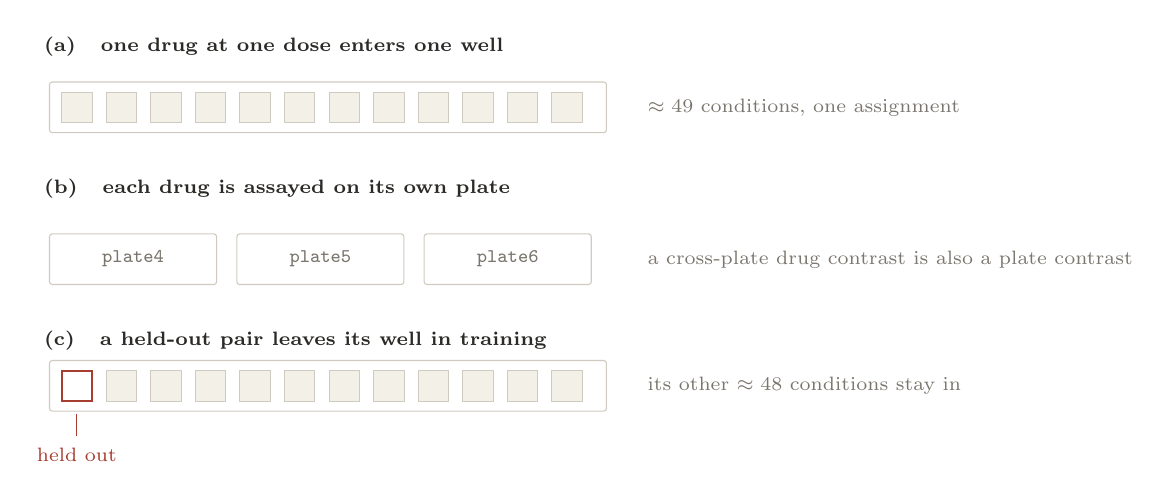
\begin{tikzpicture}[x=1.286cm, y=1.286cm, font=\small,
  lane/.style={draw=rulegrey, line width=0.4pt, rounded corners=1pt},
  cellb/.style={draw=rulegrey, line width=0.3pt, fill=panelbg,
                minimum size=3.86mm, inner sep=0pt},
  outb/.style={draw=accent, line width=0.7pt, fill=white,
               minimum size=3.86mm, inner sep=0pt},
  lbl/.style={font=\scriptsize, text=quietink},
  strong/.style={font=\scriptsize\bfseries, text=ink}]

% (a)
\node[strong, anchor=west] at (0,3.95)
  {(a)\quad one drug at one dose enters one well};
\draw[lane] (0.15,3.10) rectangle (5.65,3.60);
\foreach \i in {0,...,11}{\node[cellb] at (0.42+\i*0.44,3.35) {};}
\node[lbl, anchor=west] at (5.961,3.35)
  {$\approx 49$ conditions, one assignment};

% (b)
\node[strong, anchor=west] at (0,2.55)
  {(b)\quad each drug is assayed on its own plate};
\foreach \p/\x in {4/0.15, 5/2.00, 6/3.85}{
  \draw[lane] (\x,1.60) rectangle (\x+1.65,2.10);
  \node[lbl] at (\x+0.825,1.85) {\texttt{plate\p}};}
\node[lbl, anchor=west] at (5.961,1.85)
  {a cross-plate drug contrast is also a plate contrast};

% (c)
\node[strong, anchor=west] at (0,1.05)
  {(c)\quad a held-out pair leaves its well in training};
\draw[lane] (0.15,0.35) rectangle (5.65,0.85);
\node[outb] at (0.42,0.60) {};
\foreach \i in {1,...,11}{\node[cellb] at (0.42+\i*0.44,0.60) {};}
\draw[accent, line width=0.4pt] (0.42,0.32) -- (0.42,0.10);
\node[lbl, anchor=north, text=accent] at (0.42,0.08) {held out};
\node[lbl, anchor=west] at (5.961,0.60)
  {its other $\approx 48$ conditions stay in};

\end{tikzpicture}%
%
\end{lrbox}
\sidecap[The well is the unit the atlas actually assigns]{figure}{\captiontitle{One
assignment, many conditions.} The roughly $49$ conditions from one well share
an assignment and a batch (a). Each drug is assayed on its own plate or plates,
so a drug contrast across plates is also a plate contrast (b). Removing a (drug,
cell line) pair leaves its well in training through the other $\approx 48$ lines
(c). Squares are conditions, twelve per well for legibility.\label{fig:confound}}

\end{figure}


Dose is a molar concentration resolved from \texttt{drugname\_drugconc}; An inspection of all $289$ treated wells found $289$ usable molar doses
with zero unit collisions, so the defect was a demonstrated possibility that did
not materialise. 


\section{Barely half the atlas is identifiable}

\cref{tab:scale} states the quantities every reported sample size, $n$, in the investigation should be
located against. One symbol in it runs ahead of its
derivation.\seealso{\cref{sec:res-metrics} derives $\NIR$ and audits its chance
level with empirical control arms.} $\NIR$, the normalised inverse rank, is the
fraction of a declared comparison set whose truth a prediction resembles less
than its own, so chance is $0.50$ under the exchangeability condition of
\cref{sec:res-metrics}.

\begin{scopelimit}[carried into \cref{sec:res-blind} and \cref{sec:res-encoding}]
Two populations are used and they are not interchangeable. The broad
characterisation (\cref{sec:res-blind}) streams a wide sample of the atlas, over
more plates and drugs than cached, so the drug and condition counts in its block
of \cref{tab:scale} count that sample, not the cache. The residual arm
(\cref{sec:res-encoding} onward) works from a smaller cached subset. A count
from one block does not bound a count in the other.
\end{scopelimit}

\begin{table}[htbp]
% MARGINALIA: blocks A and B are key-value lists with dot leaders, set two-up;
% C and D stay tabular. One hairline under each block head; the five lettered
% notes and the general note set below, in the sans.
\caption{\captiontitle{The populations behind every $n$ quoted in the investigation.}
A is a streamed sample of the atlas, B the cache built once and reused. C and D
are two different evaluation schemes, keyed at different units; neither is a
subset of the other.}
\label{tab:scale}
\begin{fullwidth}
% minipage: gives the two-up blocks the full 182mm \hsize inside threeparttable
\begin{minipage}{\linewidth}
\begin{threeparttable}
\newcommand{\blockhead}[2]{\par\noindent{\thead{#1}\quad{\color{quietink}#2}}\par
  \nobreak\vspace{3pt}\noindent{\color{ink}\rule{\linewidth}{0.4pt}}\par\nobreak\vspace{6pt}}
% key-value rows as paragraphs: a long label uses the whole half-width and the
% value sits flush right on its last line, after an unbreakable dot leader.
\newcommand{\kvlead}{\nobreak{\color{rulegrey}\nobreak\cleaders\hbox to 4pt{\hss.\hss}\hskip 0.6em plus 1fill}\nobreak\hskip 0.25em\nobreak}
\newcommand{\kv}[3][0pt]{\par\noindent\leftskip=#1\relax\hangindent=0.6em\relax#2\kvlead\mbox{#3}\par}
\newcommand{\kvblock}{\RaggedRight\parskip=3pt\relax\fontsize{10.5}{13}\selectfont}
\noindent\begin{minipage}[t]{\dimexpr0.5\linewidth-6mm\relax}
\blockhead{A. Task characterisation}{streamed sample of the atlas}
\kvblock
\kv{conditions characterised}{\num{6628}}
\kv[1em]{statistically active against DMSO\tnote{a}}{3,647 / 5,014 (72.7\%)}
\kv[1em]{identifiable at the tested pseudobulk budget\tnote{b}}{3,064 (46.2\%)}
\kv[1em]{with a plate-mate closer than their own split-half}{78.7\%}
\vspace{10pt}
\kv{median cells per condition}{44}
\kv{median \#DEGs per condition (BH $q<0.05$)}{0}
\kv{median SNR (effect $\div$ within-well split-half noise)}{0.75}
\vspace{10pt}
\kv{drugs with a real dose series}{218 / 351 (62.1\%)}
\kv{drugs seen in $\geq 3$ cell lines}{227}
\end{minipage}\hfill
\begin{minipage}[t]{\dimexpr0.5\linewidth-1mm\relax}
\blockhead{B. Residual-frame cache}{rebuilt targets, \cref{sec:methods-residual}}
\kvblock
\kv{cells, treated / control}{620,564 \ (600,000 / 20,564)}
\kv{drugs / cell lines}{106 / 50}
\kv{(cell line, plate) batch groups behind them}{119}
\vspace{10pt}
\kv{conditions with $\geq 40$ treated and $\geq 20$ control cells}{6,617}
\kv[1em]{retained by the data-resolved reliability line}{2,523 of 4,999 train (50.5\%)}
\kv{training / well-held-out validation examples}{147,710 / 3,600}
\end{minipage}
\par\vspace{10pt}
\blockhead{C. Evaluation, generation and expression frames}{keyed at the (drug, cell line) pair}
\noindent\begin{tabularx}{\linewidth}{@{}Y r r r@{}}
 & \thead{Tier 1} & \thead{Tier 2} & \thead{Tier 3} \\
% MARGINALIA: the block-head hairline is this block's one rule; no \midrule.
\addlinespace[4pt]
withheld from training\tnote{c} & nothing & the drug & the pairing \\
conditions available & 4,325 & 2,188 & 99 \\
scored, generation evaluations & \multicolumn{3}{r}{400 per tier} \\
scored, expression-frame $\NIR$, within plate & & 606 & \\
\end{tabularx}
\par\vspace{10pt}
\blockhead{D. Evaluation, residual frame}{keyed at the treated well, \cref{sec:methods-holdout}}
\noindent\begin{tabularx}{\linewidth}{@{}Y r r r@{}}
 & \arm{train} & \arm{unseen_combo} & \arm{unseen_drug} \\
\addlinespace[4pt]
withheld from training & nothing & whole wells & all its wells \\
conditions after inventory filters & 4,999 & 900 & 711 \\
conditions scored, \num{1394} in all & 300 & \needsaudit{895} & 199 \\
treated wells behind them\tnote{d} & 136 & 36 & 28 \\
drugs, 90 distinct in all & 76 & 34 & 10 \\
cell lines, 42 distinct in all\tnote{e} & 39 & 42 & 40 \\
\end{tabularx}
\begin{tablenotes}[flushleft]
\item[a] Over the $5{,}014$ conditions whose (cell line, plate) group carries
plate-matched DMSO cells, not all $6{,}628$.
\item[b] Own within-plate split-half $\NIR \geq 0.8$; per-condition, and distinct
from the aggregate ceilings of \cref{tab:ceilings}.
\item[c] Tier 2 is DrEval's Leave-Drugs-Out. Tier 3 is Leave-Pairs-Out, which
\cref{sec:methods-holdout} declines as an estimand: withholding a pairing leaves
that pair's own well in training through its other $\approx 48$ cell lines.
Block D exists because of it.
\item[d] No well contributes conditions to two splits.
\item[e] Nearly every cell line appears in all three splits, by design: D
withholds wells, not lines, so it asks about an unseen treatment well of a seen
drug and never about transfer to an unseen line.
\item The \texttt{unseen\_combo} count is flagged pending a cluster rerun; no
argument turns on its exact value.
\end{tablenotes}
\end{threeparttable}
\end{minipage}
\end{fullwidth}
\end{table}

\paragraph{The upper block is a result} It describes Tahoe-100M, not this
project. Across the $5{,}014$ control-reachable conditions the median has no
differentially expressed gene at BH $q<0.05$ and a signal-to-noise ratio of
$0.75$ against its own within-well split-half noise, while $72.7\%$ are active
on the whole profile, leaving $27.3\%$ statistically inert. A per-gene test is
far harsher, and $27.3\%$ alone would make the atlas sound better resolved than
it is. The typical condition carries a real response
measured with too few cells, and not no response (\cref{sec:res-blind}).

The identifiability bar is per-condition: a condition's own split-half $\NIR$
against its plate-mates has to clear $0.8$. Of the $6{,}628$ conditions,
$46.2\%$ clear it, and $78.7\%$ have a plate-mate lying closer to them than
their own second half does. Identifiability is a property of the pairing, not of
the drug: over the $227$ drugs assayed in at least three cell lines, the median
drug's split-half reference spans $0.83$ between its most and least identifiable
context. A benchmark omitting those figures
quotes accuracies over a population barely half of which is empirically
identifiable at the tested pseudobulk budget, and a per-drug leaderboard on it
ranks pairings.

% The term is first used in tab:scale above, inside a float, where a marginpar
% cannot be set. This is its first prose use and the chapter's definition point,
% per the \gloss convention (definition at first use in each chapter). Wording
% is the one 05-Limitations.tex already uses, so the two agree word for word.

The three tiers of the last block are defined by what training contained.
\emph{Tier 1} holds conditions whose (drug, cell line) pairing was
seen in training, so it measures fit and not generalisation. \emph{Tier 2} holds
conditions whose drug never appeared, Leave-Drugs-Out in the vocabulary of
\cref{sec:lit-dreval}. \emph{Tier 3} holds pairings whose drug and cell line
were each seen but never together, Leave-Pairs-Out; it is small ($99$
conditions) and is reported only where adequately powered. The residual arm
builds its own, larger holdout instead: \cref{sec:apparatus-vocab} names its
three splits, and \cref{sec:methods-holdout} settles the unit they are keyed
at.

\section{The backbone has seen no perturbation}

A cell is written as a \emph{cell sentence}, its expressed panel genes in
descending order, terminated by \ENDCELL{}, which is registered as an atomic
special token. The prompt supplies cell line, drug, dose, mechanism and the
control cell's sentence; what the model must produce is the treated cell's. 

The terminator is not inherited. A cell expresses only part of the panel, so
sentences differ in length, and a model with no way to mark where its expressed
list ends leaves the boundary between what it ranked and what it omitted to be
inferred from the output. An earlier build here removed the problem rather than
solving it, writing all $946$ panel genes with the unexpressed appended in a
fixed tail: nothing was ever absent, so every convention for handling absence
collapsed into the same one, and most of the generation budget went on a tail
that carried no information. This build lists only what is expressed and closes
it with \ENDCELL{}, an atomic special token registered in the trainer, so a
sentence is variable in length and its end is declared rather than deduced.
Stripping the tail without a marker would have left the same inference to be made
silently. Absence is now a real property of a prediction, which is also why the
rank-based metrics of \cref{sec:res-metrics} need a stated convention for it.

The backbone is \texttt{C2S-Scale-Pythia-1b-pt}~\cite{c2sscale}, a C2S-Scale
checkpoint on the Pythia-1b decoder~\cite{pythia}, cold-started for every arm
from the same base checkpoint with identical hyperparameters (1 epoch, learning
rate $10^{-5}$, gradient accumulation 16, maximum length 8192,
bf16).\seealso{\cref{sec:appendix} tabulates the training arms.} Cold-starting
makes the arms comparable; the training target or objective is the only
variable.

\paragraph{What the checkpoint has seen} It is pretrained on over 50 million
human and mouse cells from 825 single-cell datasets in CELLxGENE and the Human
Cell Atlas, an atlas corpus with no chemical or genetic perturbation data. Its
model card lists cell and tissue prediction, conditioned generation and gene-set
conversion, but not perturbation prediction. The base model arrives at
fine-tuning here having never seen a drug-treated cell.

\paragraph{Two channels stay open} The decoder underneath is Pythia-1b,
pretrained on text in which drug names, targets and mechanisms occur, and every
prompt supplies the drug's \texttt{moa-fine} annotation. A drug the fine-tuning
never saw is not a drug the system knows nothing about.

\begin{scopelimit}[carried into \cref{sec:res-scope} and \cref{sec:limitations}]
``Held out'' therefore means held out from Tahoe fine-tuning, with mechanism
supplied, and every unseen-drug result below is read under that narrower scope.
\end{scopelimit}

\paragraph{Which leaves the target} Two facts sit together here. The checkpoint
has never seen a drug-treated cell, so whatever it comes to know about
perturbation it learns during fine-tuning and learns from the target it is given.
And the formulation it inherits was written for a different job, producing a
plausible cell rather than producing a drug specific treated cell. Cold-starting
fixes the model, so the target is the only thing left that can be moved, and
whether it should be is the question \cref{sec:apparatus-vocab} takes up.

\section{The training target decides the frame}
\label{sec:apparatus-vocab}

The model and the prompt are now fixed, so the string the model is trained to
produce is the only thing left that varies. Two constructions of it run through
the investigation. They are choices about how the target is built and not about
the model, and each carries with it the object a score is taken on, the
competitors it is taken against, and the function that compares them. That triple
is what is called a \emph{measurement frame} here.

\paragraph{The inherited target} The first is the formulation C2S-Scale defines
for perturbation prediction, kept unchanged. The target is the treated cell's
own sentence, its expressed panel genes in descending order, and nothing is
subtracted from it. It is a general-purpose construction, written for a model
asked to produce a plausible cell rather than to tell two treatments apart, and
it is what makes the comparison of \cref{sec:lit-c2s} possible at all.

\paragraph{The perturbation-specific target} The second is built for this
question, because the first one hides the drug: two different drugs on the same cells give
almost the same target string, making it a fault of the data that the model can't give drug specific predictions instead of the model itself.  \Cref{sec:methods-residual} is the measurement
that motivates replacing it. Two subtractions turn a treated profile into a
drug-specific one.

\begin{defn}{The shift, the generic and the drug-specific residual}
For a condition $c$, a (drug, cell line, plate, dose) tuple with at least $40$
treated and $20$ plate-matched control cells, write $d$ for its drug and
\begin{equation}
 \resid(d,c) \;=\;
 \underbrace{\big(\bar{y}_{\textrm{treated}} - \bar{y}_{\textrm{control}}\big)}_{\shift(d,c)}
 \;-\;
 \underbrace{\frac{1}{|D_c \setminus \{d\}|}
   \sum_{d' \in D_c,\; d' \neq d} \shift(d',c)}_{\textrm{generic}(c)} .
\end{equation}
Both bars are pseudobulks: $\bar{y}_{\textrm{treated}}$ averages the condition's
own treated cells and $\bar{y}_{\textrm{control}}$ its plate-matched controls, so
$\resid(d,c)$ is one vector for the whole condition and not a quantity carried by
any single cell. The control subtraction removes the state those cells share,
leaving the \emph{shift}. The mean over the other drugs removes the \emph{generic}
programme every drug triggers, conventionally read as a shared stress and
cell-cycle response, a reading used here for intuition and nowhere tested. What
survives both subtractions is the \emph{drug-specific residual}, and taking it as
the string the model is trained to emit makes it the \emph{residual target}. A
condition therefore supplies many training examples but only one target: the
prompt varies from one plate-matched control cell to the next, and every one of
them is paired with the same residual string.

\smallskip
$D_c$ is the training drugs sharing $c$'s (cell line, plate) group, each drug
entering once whatever its doses. That grouping is the generic's \emph{scope},
and this build takes it at plate scope; \cref{sec:res-transfer} reports the
cell-line-scoped alternative alongside it. Two properties of $D_c$ are fundamental. It is \emph{split-before-fit}: the holdout is fixed from metadata
before any statistic is estimated, the generic included. And it is
\emph{leave-one-drug-out}: a condition's own drug never enters its own generic,
so the subtraction removes what the other drugs share and cannot remove the drug
being predicted.

\smallskip
The scope is also the limit. What remains is not what makes this drug different
from all drugs. It is what makes it different \emph{from the other training
drugs that happen to share its plate and cell line}.
\end{defn}
\paragraph{Writing the residual as a string} $\resid(d,c)$ is a signed vector
over the panel, and a decoder emits tokens rather than vectors, so the target has
to be written down before it can be trained on. The obvious form is the wrong
one. A single list in descending order buries the most strongly repressed genes
at the tail, among the genes the drug did not move at all, and repression is
exactly what the control subtraction was performed to expose. The sign is the
biology, so the encoding keeps it: the target is two ordered blocks, the most
up-regulated genes first, a \DOWN{} separator, then the most down-regulated
genes, closed by \ENDCELL{}. Up to $100$ genes enter each block, which is the
$200$ target positions \cref{tab:divergence} counts over, and a gene enters a
block only if its residual actually carries that sign, so a condition with few
movers emits a short one. \DOWN{} is registered as an atomic special token
alongside \ENDCELL{}; unregistered it splits into sub-words and the up/down
boundary stops being a clean symbol. What the model is asked to produce is
therefore a ranked signed signature, not a cell.

\paragraph{Reading a generation back, in each frame} What the model emits is a
string, and a similarity needs vectors, so a generation --- and the truth it is
scored against --- has to be read back into one. Three read-backs are used below,
and which one applies is a property of the metric and not of the frame: the frame
names the object scored, a cell profile or a residual, and not the units it is
scored in.

The first leaves the sentence where it is. A gene's value is its position in the
sentence, counting from one, and a panel gene the sentence omits takes the rank
the absent-gene convention assigns (\cref{sec:app-convention}). $\DEdr$ and
$\paneltau$ are computed here and never leave rank space.

The second decodes to a reconstructed expression profile. Write $p_g$ for the
position at which gene $g$ appears. Then
\begin{equation}
 \psi(s)_g \;=\;
 \begin{cases}
   \max\!\big(0,\; a\log_{10} p_g + b\big) & \text{if $g$ appears in $s$},\\[2pt]
   0 & \text{if $g$ does not,}
 \end{cases}
\end{equation}
with $a$ and $b$ a single slope and intercept fitted once for the whole run
(\cref{sec:lit-c2s}). This is what \texttt{nir\_expr} reads, prediction and truth
both decoded, and it is the only read-back that invents a magnitude. Note that
the absent-gene convention does not reach it: $\psi$ fills an omitted gene with
zero whatever the convention says.

The third keeps only sign and order, because a residual has no expression units to
decode into. Write $s$ for a signed signature of either kind, and let $U(s)$ and
$D(s)$ be its up and its down block: for a generation, the two lists the model
emitted, in the order it emitted them; for a continuous residual, its most
positive and its most negative entries under the same cut of $100$. Let $r_g$ be
the position of gene $g$ within whichever block holds it, counting from one. Then
\begin{equation}
 \phi(s)_g \;=\;
 \begin{cases}
   +\,1/\log_{2}(r_g + 1) & \text{if } g \in U(s),\\[2pt]
   -\,1/\log_{2}(r_g + 1) & \text{if } g \in D(s),\\[2pt]
   0 & \text{if $g$ is in neither block.}
 \end{cases}
\end{equation}
The leading gene of each block carries weight one and the weight falls away down
the block, so a gene's rank is all that reaches the vector and the value that
earned it that rank is discarded. The discount is what makes the ordering inside a
block count for something --- agreeing on the most up-regulated gene is worth more
than agreeing on the hundredth, where one rank is barely distinguishable from its
neighbours, and a flat encoding would score those two agreements alike.

All three read position and nothing else. A gene's identity decides \emph{where}
a value lands in the vector, never \emph{what} that value is, and all three fill
with zero or with a convention whatever the string leaves out. They differ in what
they then claim: $\psi$ writes position into expression units through a map fitted
to data, so an expression-frame distance taken on it is a distance between two
reconstructions; $\phi$ writes position into fixed weights that no fitting
produced, so a residual-frame comparison is a rank-weighted overlap of gene sets
and carries no units at all. \Cref{tab:sigma} records which read-back each quoted
figure rests on.
\paragraph{Why the target carries a frame with it} A model trained on the first
target emits a cell profile; a model trained on the second emits a signed
up-and-down signature. The two are not the same kind of object, and neither
scoring path accepts the other's output: the rank-to-expression decode is fitted
for expression ranks and its truths are full pseudobulks, while a residual
signature has no expression units to decode into. So the choice of target
settles the space a prediction lives in, and a score has to be taken in that
space or not at all. Comparing a number from one frame with a number from the
other is the most expensive misreading this thesis allows.

Both frames score by discrimination and not by proximity. A prediction is never
asked how close it came to its own truth. It is set beside a lineup of other
conditions' truths and asked whether it resembles its own more than it resembles
any of theirs. That fraction is the \emph{normalised inverse rank}
$\NIR$,\seealso{\cref{sec:res-metrics} derives $\NIR$ and audits its chance level
with empirical control arms.} and the lineup is the \emph{comparison set} $J$.
Choosing $J$ is a substantive decision rather than a formality: anything every
candidate in $J$ has in common cannot help a prediction win, because it is
equally true of all of them. Narrowing $J$ is how a nuisance cue is switched off.

The two frames narrow it differently. The \Eframe{} \emph{expression frame}
scores the inherited target's output, a predicted cell profile, against the other
drugs \emph{on its own plate}, so every candidate carries the same batch and no
prediction can score by recognising the plate it came from --- a leak
\cref{sec:res-blind} measures rather than assumes. The \Rframe{} \emph{residual
frame} scores the residual target's output against the other drugs \emph{in its
own cell line}, more widely scoped than the generic, so every candidate carries
the same cellular background and the drug is the only thing left to separate
them. Chance sits at $0.50$ in both, under an exchangeability condition
\cref{sec:res-metrics} tests with control arms instead of assuming, and $J$ is
declared at every score below. A score without its comparison set is not a score.

The \emph{similarity} $\sigma$, the function by which a prediction is judged
closer to one truth than to another, is the third thing the target settles, and
it follows neither from the scored object nor from the comparison set on its own:
a negated Euclidean distance on decoded expression in the expression frame, a
cosine on the signed rank-discounted residual in the residual frame, the two
instances \cref{tab:sigma} fixes with their comparison sets. A score without its
similarity is not a score either, and both are to be declared before a number is
read.

% ===========================================================================
% frames.tex -- the two measurement frames, EXPR and RESID, as two cards.
% \input by Sections/03-Apparatus.tex. Compiles against thesis_v2/preamble.tex
% and nothing else; no external data, no \includegraphics.
%
% NO DATA SOURCE. This is a schematic. The only numeral on the cards is the
% chance level 0.50, which is a definition and not a measurement: both frames
% are two-alternative retrievals, so chance is 0.50 by construction. It agrees
% with the prose immediately above this figure in Sections/03-Apparatus.tex
% ("Both put chance at $0.50$"), with Sections/02-Background.tex:244 and with
% Sections/04a-ruler.tex:530 ("Chance is $0.50$ by ..."). Nothing here is read
% from RESULTS_cluster/ because nothing here is a result. The numeric version
% of this argument -- the two frames on their own scales -- is fig:two-scales
% in 04d; Chapter 3 is apparatus and comes before those results exist, so this
% figure carries no scale, no axis and no measured quantity. Sibling
% frames.json records the geometry and that single number.
%
% ---------------------------------------------------------------------------
% THE BUG, AND WHY THE FIX IS NOT THE ONE-LINER IT LOOKS LIKE.
%
% Symptom, both cards: the two-line value on row 2 collided with its own key.
% Measured in the built thesis, ink gap between the key and its value, in
% PostScript points: r1 -0.02, r2 -3.02, r3 +2.12. Only r2 is visible as a
% collision. (r1 is the descender of "predicted" level with the ascender of
% "profile"; different x, they do not touch.)
%
% Diagnosis, as briefed and confirmed: val/.style used anchor=WEST, which
% centres a node's box on its y, so a TWO-LINE value grew upward into the key
% above it while one-line values did not.
%
% The briefed fix was anchor=north west with every value at its key's
% y - 0.30cm. Built, that removes the collision and introduces a worse fault:
% it lowers each value until it sits CLOSER TO THE NEXT KEY THAN TO ITS OWN,
% so every value reads as the heading of the row beneath it. Sweeping the
% offset, all measured inside one PDF by tools/_measure_frames.py and recorded
% in frames.json, gave "within" = key to its own value, "between" = value to
% the next key:
%
%   offset      within r1 / r2 / r3      between: after r1 / after r2
%   0.15          2.21  2.24  3.14            9.60        7.43
%   0.30          6.46  6.49  7.39            5.35        3.18   <- reversed
%   0.40          9.29  9.33 10.23            2.51        0.35
%
% and then the same figure BUILT INSIDE THE THESIS at offset 0.15 measured
% 5.95 / 5.98 / 5.29 within against 5.86 / 3.69 between -- 3.7pt away from the
% harness, and ambiguous. The offset is not a constant of the figure.
%
% ROOT CAUSE, and why this file no longer uses align=left. TikZ's `align'
% option typesets the node in a minipage, and a minipage's first-line height
% follows the AMBIENT \baselineskip. So a value node's ink lands in a place
% that depends on the prose that happens to precede the float: about 2.2pt
% between a \normalsize paragraph and a \small line, and about 3.7pt between a
% test harness and Chapter 3. No choice of offset survives an edit to the
% surrounding text. Calibrating one would have hidden the fault, not fixed it.
%
% THE FIX ACTUALLY USED: every node is a single line anchored BASE WEST, so
% each y coordinate below IS that line's baseline. Nothing is centred, nothing
% is measured from a box edge, no minipage is created, and no ascender or
% descender can move a line. The two-line value is two nodes rather than one
% node with `\\'. Key-to-value leading is therefore identical on all three rows
% and on both cards by construction -- which is what the brief asked for -- and
% it is now also identical from build to build.
%
%   key baselines    3.70   2.72   1.52     (row pitch unchanged)
%   value baselines  3.37   2.39   1.19     (key - 0.33cm)
%   row-2 value, second line  2.06          (previous line - 0.33cm)
%
% ONE step governs everything inside a row: 0.33cm = 9.39pt, one \scriptsize
% line of leading. A key and its value therefore set as two consecutive lines
% of a single block, exactly as rows 1 and 3 of the published figure did, and a
% wrapped value continues on the same rhythm. Row SEPARATION is carried
% entirely by the key pitch, which is untouched (0.98cm, then 1.20cm), giving
% 0.65cm and 0.53cm of clear space before the next key -- roughly twice the
% within-row step, so a value binds to the key above it and not to the one
% below.
%
% Verified by reading the baselines back out of the built PDFs. Chapter 3 in
% main.pdf and all four contexts of figs/_frames_harness.tex report the same
% seven baselines to 0.001cm:
%   3.703  3.375 | 2.727  2.398  2.059 | 1.531  1.203   (tikz y, both cards)
% Note the harness and the thesis are only comparable on BASELINES. Glyph
% bounding boxes reported by a PDF text extractor differ by a constant ~2.1pt
% between the two files because the font subsets differ, so ink-gap numbers
% are only meaningful WITHIN one PDF.
%
% OTHER LAYOUT NOTES
%   * cards are 5.9cm wide with a 0.5cm gutter, 12.3cm overall. NOT rescaled:
%     12.3cm sits inside the 14.2cm body block and leaves the page free to
%     carry a margin note.
%   * the dotted rule and the sentence under it span BOTH cards on purpose.
%     They are the only mark that crosses the gutter; everything else is
%     card-local, because the point of the figure is that the columns do not
%     exchange.
%   * if a value ever needs a third line, add a node at (its predecessor
%     - 0.34cm). Do not reintroduce align/`\\'.
% ===========================================================================
\begin{figure}[htbp]
% MARGINALIA (06-figures.md): no borders on the two cards; the frame names are
% sans tags in accent; the figure fits the text column, so its caption is in
% the margin (\sidecap).
\begin{lrbox}{\tvfb}%
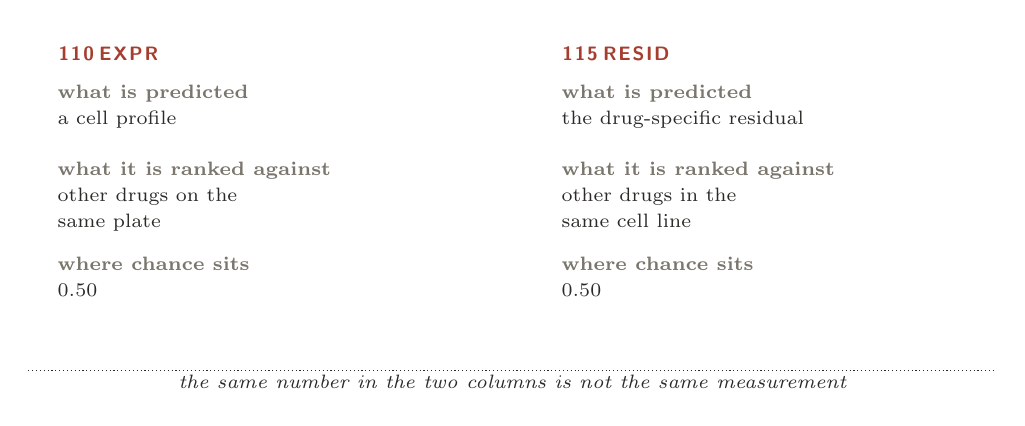
\begin{tikzpicture}[x=1cm, y=1cm, font=\small,
  panel/.style={draw=none},
  % base west on both: every y below is a BASELINE. See the header note --
  % anchor=west centres the box (that was the collision) and align=left makes
  % the node's height depend on the surrounding prose (that was worse).
  key/.style={font=\scriptsize\bfseries, text=quietink, anchor=base west},
  val/.style={font=\scriptsize, text=ink, anchor=base west}]

\draw[panel] (0,0.55) rectangle (5.9,4.6);
\draw[panel] (6.4,0.55) rectangle (12.3,4.6);

\node[anchor=base west] at (0.25,4.18)
  {{\sffamily\fontsize{7.5}{9}\selectfont\bfseries\color{accent}\textls[80]{\ding{110}\,EXPR}}};
\node[anchor=base west] at (6.65,4.18)
  {{\sffamily\fontsize{7.5}{9}\selectfont\bfseries\color{accent}\textls[80]{\ding{115}\,RESID}}};

% key baseline 3.70 / 2.72 / 1.52 ; value baseline = key - 0.33 ; wrap - 0.34.
\node[key] at (0.25,3.70) {what is predicted};
\node[val] at (0.25,3.37) {a cell profile};
\node[key] at (6.65,3.70) {what is predicted};
\node[val] at (6.65,3.37) {the drug-specific residual};

\node[key] at (0.25,2.72) {what it is ranked against};
\node[val] at (0.25,2.39) {other drugs on the};
\node[val] at (0.25,2.06) {same plate};
\node[key] at (6.65,2.72) {what it is ranked against};
\node[val] at (6.65,2.39) {other drugs in the};
\node[val] at (6.65,2.06) {same cell line};

\node[key] at (0.25,1.52) {where chance sits};
\node[val] at (0.25,1.19) {$0.50$};
\node[key] at (6.65,1.52) {where chance sits};
\node[val] at (6.65,1.19) {$0.50$};

\draw[ink, line width=0.4pt, densely dotted] (0,0.25) -- (12.3,0.25);
\node[font=\scriptsize\itshape, text=ink, anchor=base] at (6.15,0.02)
  {the same number in the two columns is not the same measurement};
\end{tikzpicture}%
\end{lrbox}
\sidecap[The two measurement frames]{figure}{\captiontitle{Two frames, one chance level, and
no exchange rate between them.} The prediction, the comparison set and the
meaning of a score change between frames; the chance level does not.\label{fig:frames}}
\end{figure}


\section{One estimator, and not a replicate}

Almost every negative result below is stated as a distance from a
\emph{ceiling}. 

\begin{defn}{Within-well split-half precision reference}
The score obtained when a disjoint cell subset of the same treated well is
substituted for the prediction, recomputed for every stratum scored, so its
value moves with the stratum. It is not a replicate ceiling. What varies across
the rows of \cref{tab:ceilings} is the frame, the comparison set and the cell
budget, never the estimator.
\end{defn}

Two properties limit how the ceilings read. First, they are \emph{split-half}
estimates and not biological replicates, because this cache places $286$ of
$287$ treatments in exactly one well. Second, a split-half ceiling estimates
within-well sampling precision, which is optimistic relative to true biological
reproducibility, and every coverage figure in \cref{sec:res-lookup} inherits
that optimism.

\paragraph{The one exception} One ceiling is not that estimator and not a row in
\cref{tab:ceilings}. The positive control inside the expression-frame $\DRF$
audit of \cref{sec:res-metrics} is a denoised interpolated duplicate, not a raw
split-half, and that section turns on the difference.

\begin{table}[htbp]
% MARGINALIA: full width; caption above at the text width, notes below in the
% sans. Text columns widened so every metric description fits on two lines.
\caption{\captiontitle{One estimator, seven settings.} Every ``ceiling'' here is a
within-well split-half precision reference, the score of a disjoint subset of
the same treated well's cells. They differ in frame, comparison set, cell budget
and split contents.}
\label{tab:ceilings}
\begin{fullwidth}
\begin{threeparttable}
\begin{tabularx}{\linewidth}{@{}r L{61mm} L{48mm} Y@{}}
\thead{Ceiling} & \thead{Frame and metric} & \thead{Comparison set and budget}
  & \thead{Where used} \\
\midrule
$0.76$ & expression, $\DEdr$ & two real cells & metric audit
  (\cref{sec:res-metrics}) \\
\addlinespace
$0.625$ / $0.575$ & expression, $\NIR$ (negated Euclidean on decoded expression)
  & leak audit; cross-plate / within plate
  & plate leak (\cref{sec:res-blind}) \\
\addlinespace
$0.67$--$0.83$ & expression, forced choice & within plate, by cell budget
  & \cref{sec:res-blind} \\
\addlinespace
$0.576$ & expression, $\NIR$ (negated Euclidean on decoded expression)
  & within plate, tier 2 & the blindness verdict \\
\addlinespace
$0.61$ / $0.76$ / $0.85$ & expression, $\NIR$ (negated Euclidean on raw
  pseudobulk, undecoded) & \emph{cross-plate};
  $10$/$40$/$120$ cells & identifiability curve \\
\addlinespace
$0.956$/$0.824$/$0.836$ & residual, $\NIR$ (cosine on the signed rank-discounted
  residual) & within cell line;
  train/combo/drug & \cref{sec:res-lookup} \\
\addlinespace
$0.742$ / $0.7432$ & retrieval, negated Euclidean on undecoded log-expression
  & within condition, split-half
  & \cref{sec:methods-residual} \\
\end{tabularx}
\begin{tablenotes}[flushleft]
\item The $\DRF$ positive control of \cref{sec:res-metrics} is the
investigation's one exception and is not a row here.
\item None of these is a biological replicate ($286$ of $287$ treatments sit in
a single well).
\item In the residual frame the raw reference is not constant across splits (a
spread of $0.132$), but that spread is an artefact of how the splits were
filtered and not a difference in recoverable signal; matched at the training
reliability line the three agree to $0.006$ (\cref{sec:limitations}).
\end{tablenotes}
\end{threeparttable}
\end{fullwidth}
\end{table}

\begin{scopelimit}[carried into \cref{sec:res-lookup} and \cref{sec:limitations}]
A distance to the reference is comparable within a split and not between them,
because the splits are scored on populations selected by different rules. And
because the reference is a sampling-precision estimate and not a biological
replicate, every coverage figure computed against it is a distance to an
optimistic bar by an unknown amount. Where one is quoted, the ordering carries
the claim.
\end{scopelimit}

\section{Two crossed dependencies, not one}
\label{sec:apparatus-clusters}

Two rules apply to every result below, plus one statement of provisionality.
Conditions are not independent, and not independent in two crossed ways at once
(\cref{fig:clustering}): two from one treated well share a physical assignment
and a batch, two from one cell line share the biology. Treating them as
independent gives intervals about $1.5$ times too narrow on the scramble
strata and $1.7$ to $2.5$ times too narrow on the contrasts against the lookup
baselines. Clustering on the assignment unit alone uses the larger cluster
count ($289$ wells against $\approx 50$ lines) and would tighten every interval
while sounding more rigorous. That is the failure the estimator below avoids.

% ===========================================================================
% clustering.tex -- the two crossed groupings, plus the drug the wells nest in.
% \input by Sections/03-Apparatus.tex. Compiles against thesis_v2/preamble.tex
% and nothing else; SCHEMATIC -- no external data, no \includegraphics, and
% deliberately NO number anywhere in the drawing. The lattice is 9 columns of
% 6 dots because that is what reads at this measure, not because the cache
% holds 9 wells or 6 lines; the caption says so in as many words.
%
% WHY IT WAS REDRAWN. The version it replaces sat inline in 03-Apparatus.tex
% at lines 477-510 (v1's is under ../thesis/ and is not touched).
%
%   1. THE DOT WAS NOT ON THE LATTICE. The old bands were centred at y=2.6 and
%      x=5.0, while the lattice rows sat at 0.5+0.6r (2.3, 2.9) and the columns
%      at 0.7+1.1c (4.0, 5.1). Both centre lines fell BETWEEN dots, so the
%      accent "one condition" dot was drawn in the gap. The caption said "the
%      dot where they meet is one condition" and the drawing did not show one.
%      Here every coordinate is derived from the two constants the lattice is
%      generated from (\px, \py) and the highlight is addressed by INDEX
%      (\hc, \hr), so band centres and accent dot cannot drift off a lattice
%      point again.
%
%   2. THE BANDS WERE PADDED BY EYE. Old horizontal band 0.35..8.45 against
%      dots at 0.7..7.3 -- 0.35 short at the left, 1.15 long at the right. Old
%      vertical band 0.12..4.08 against dots at 0.5..4.1 -- 0.38 short at the
%      bottom, 0.02 over at the top. Here each band ends exactly half a lattice
%      pitch past its first and last dot (\BL,\BR,\BB,\BT below), computed, so
%      both are symmetric by construction.
%
%   3. THE DOTS WERE TEXTURE, NOT CONDITIONS. They were rulegrey!70, i.e.
%      #9A9A9A at 70% over white ~= #C0C0C0 -- lighter than the document's
%      quiet ink and far too light for a mark the caption asks the reader to
%      count. They are quietink (#6B6B6B) here, and 1.7pt rather than 1.5pt.
%
%   4. IT PAID FOR FULLWIDTH AND DID NOT USE IT. The old float opened
%      \begin{fullwidth} -- 174mm, and by the preamble's own rule a page
%      carrying one may then carry no margin note -- and drew 148.6mm. This
%      draws inside the 142mm measure (see MEASURED below), so it is an
%      ordinary body-width float and its page keeps the margin column.
%
%   5. THE DRUG WAS IN NO FIGURE AT ALL, and it is the axis that flips three
%      verdicts later. It is drawn in a deliberately different register from
%      the two bands: outline only, no fill, rounded corners, against two solid
%      tint rectangles. A well carries one drug at one dose (sec. "Every
%      treatment sits in one well"), so wells NEST inside drugs -- three whole
%      well-columns per envelope -- while the cell-line band CROSSES all three
%      envelopes and runs past the outer edge of both end ones. Nesting and
%      crossing are then the same picture, told apart by shape, not by colour.
%
% GEOMETRY, in cm, all of it derived from \px and \py. Every clearance here is
% computed from those two constants, not judged by eye:
%   lattice     9 cols x 6 rows, pitch 1.25 x 0.81, dots (0,0)..(10.00,4.05)
%   highlight   col 4 -> x = 5.00, row 4 -> y = 3.24     <- both ON the lattice
%   bands       half-thickness 0.25, so 0.155 of ground to the next dot row
%               (0.405 half-pitch - 0.25) and 0.095 clear of that dot's edge;
%               ends at -0.625/10.625 and -0.405/4.455, i.e. exactly half a
%               pitch past the first and last dot of the row and the column
%   envelopes   3 x 3 columns, pad 0.46 -> -0.46..2.96, 3.29..6.71, 7.04..10.46,
%               so 0.33 between neighbours; vertically -0.585..4.635, giving
%               0.18 of margin above and below the well band each one contains
%   callout     the leader leaves the accent dot at 46.3 deg, clears the
%               nearest lattice dot (6.25,4.05) by 0.354, and crosses the
%               middle envelope's TOP edge at x = 6.32, inside that envelope's
%               span 3.29..6.71 -- so it pierces one boundary and not two
%
% MEASURED, not estimated. figs/_harness_clustering.tex \input s this file
% against the real preamble, captures the float into a box with \caption and
% \label gobbled, and \typeout s \wd. Reading:
%   tikzpicture  385.40pt = 135.45mm wide, 187.44pt = 65.87mm tall
%   \textwidth   404.03pt = 142.00mm
%   fills 95.4% of the measure, 18.63pt = 6.55mm of slack.
% The build's overfull-hbox gate is 0; this figure contributes none. The
% fullwidth version it replaces drew 148.6mm against a 174mm allowance -- it
% overran the body measure, which is why it was in a fullwidth in the first
% place, and cost that page its margin column to do it.
%
% TYPE. \scriptsize on every label, matching fig:confound three pages earlier
% and fig:residual-energy in chapter 4. Deliberately not raised: this figure is
% read alongside fig:confound, and a lone larger label set would read as a
% different apparatus rather than as a corrected one.
% ===========================================================================
\begin{figure}[htbp]
% MARGINALIA (06-figures.md): fits the text column; caption in the margin.
\begin{lrbox}{\tvfb}%
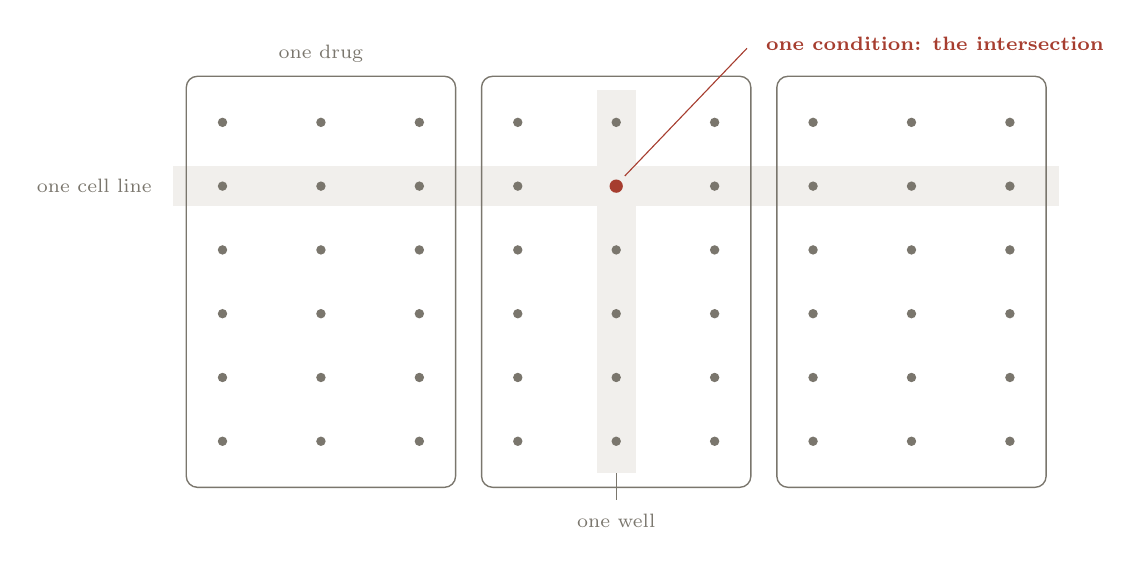
\begin{tikzpicture}[x=1cm, y=1cm, font=\small]
  % --- the constants everything else is derived from -----------------------
  \def\px{1.25}   % column pitch  (one well per column)
  \def\py{0.81}   % row pitch     (one cell line per row)
  \def\hc{4}      % highlighted column index, 0..8
  \def\hr{4}      % highlighted row index,    0..5
  \def\bt{0.25}   % half band thickness
  \def\ep{0.46}   % envelope padding around its three columns
  \def\vm{0.18}   % envelope margin above and below the well band

  \tikzset{
    cond/.style={fill=quietink},
    band/.style={fill=rulegrey!30},
    drugenv/.style={draw=quietink, line width=0.5pt, rounded corners=4pt},
    lead/.style={draw=quietink, line width=0.4pt},
    lbl/.style={font=\scriptsize, text=quietink},
    strong/.style={font=\scriptsize\bfseries, text=accent}}

  % centre lines of the two bands: ON the lattice, by construction
  \pgfmathsetmacro{\HX}{\hc*\px}            %  5.000
  \pgfmathsetmacro{\HY}{\hr*\py}            %  3.240
  % band ends: half a pitch past the first and last dot, both sides, both bands
  \pgfmathsetmacro{\BL}{-\px/2}             % -0.625
  \pgfmathsetmacro{\BR}{8*\px+\px/2}        % 10.625
  \pgfmathsetmacro{\BB}{-\py/2}             % -0.405
  \pgfmathsetmacro{\BT}{5*\py+\py/2}        %  4.455
  \pgfmathsetmacro{\EB}{\BB-\vm}            % -0.585
  \pgfmathsetmacro{\ET}{\BT+\vm}            %  4.635

  % ---- 1. the two crossed groupings, as solid tint bands ------------------
  \fill[band] (\BL,\HY-\bt) rectangle (\BR,\HY+\bt);      % one cell line
  \fill[band] (\HX-\bt,\BB) rectangle (\HX+\bt,\BT);      % one well

  % ---- 2. the drug, as an outline envelope over three whole well-columns --
  % It encloses the well band top and bottom as well as left and right, so the
  % well reads as INSIDE the drug and not merely beside it.
  \foreach \g in {0,1,2}{
    \pgfmathsetmacro{\GL}{3*\g*\px-\ep}
    \pgfmathsetmacro{\GR}{(3*\g+2)*\px+\ep}
    \draw[drugenv] (\GL,\EB) rectangle (\GR,\ET);}

  % ---- 3. the conditions --------------------------------------------------
  \foreach \c in {0,...,8}{
    \foreach \r in {0,...,5}{
      \fill[cond] (\c*\px,\r*\py) circle (1.7pt);}}

  % ---- 4. the intersection ------------------------------------------------
  \fill[accent] (\HX,\HY) circle (2.4pt);
  \draw[accent, line width=0.4pt]
    (\HX+0.11,\HY+0.13) -- (\HX+1.66,\HY+1.75);
  \node[strong, anchor=west] at (\HX+1.78,\HY+1.81)
    {one condition: the intersection};

  % ---- 5. direct labels, one per grouping. No legend, no key. -------------
  % cell line: to the left of its own band.
  \node[lbl, anchor=east] at (\BL-0.15,\HY) {one cell line};

  % well: below its own band, on a lead that PIERCES the envelope's lower
  % edge -- the crossing of that boundary is the nesting, drawn.
  \draw[lead] (\HX,\BB) -- (\HX,\BB-0.34);
  \node[lbl, anchor=north] at (\HX,\BB-0.40) {one well};

  % drug: above the leftmost envelope, centred on it. Placed there and not on
  % the middle envelope because the middle one is where the well band and the
  % callout leader already are, and "one drug" centred over the highlighted
  % column would compete with "one well" for the same column.
  \node[lbl, anchor=south] at (\px,\ET+0.06) {one drug};

  % NO free-floating note line. The version this replaces carried "neither
  % grouping is nested in the other" as a caption-width sentence under the
  % lattice. Two reasons it is gone: the caption now states it in the same
  % words, and at page scale a \scriptsize sentence sitting 4mm above
  % "Figure 3.3." reads as the caption's first line rather than as part of the
  % drawing. The claim is not dropped -- it moved into the caption, where the
  % new drug clause needs it anyway.
\end{tikzpicture}%
\end{lrbox}
\sidecap[The two crossed groupings, and the drug the wells nest in]{figure}{\captiontitle{A
condition belongs to a well and to a cell line at once, and the two groupings
cross.} Each dot is a condition; the horizontal band is one cell line, the
vertical band one well. The dot where they meet is one condition, which is why
the intersection term is the ordinary independent-sampling variance. The
rounded envelopes are drugs: a well carries one drug at one dose, so wells nest
inside drugs, while the cell-line band crosses every drug and neither of the
two bands is nested in the other. The lattice is schematic --- nine columns of
six, for legibility, and not a count of anything in the cache.\label{fig:clustering}}

\end{figure}


Every interval on a \emph{mean} is therefore two-way cluster-robust
(Cameron--Gelbach--Miller),
\begin{equation}
 V \;=\; V_{\textrm{line}} \;+\; V_{\textrm{well}} \;-\; V_{\textrm{intersection}},
\end{equation}
where the intersection of the two groupings is the single condition, so
$V_{\textrm{intersection}}$ is the ordinary independent-sampling variance. When
it goes non-positive in a finite sample, the wider one-way variance is used and
the branch recorded. The formula above is valid only where the two groupings
genuinely cross, which cell line and well do: a treated well spans
$\approx 49$ cell lines and a cell line recurs across wells. Drug and well do
\emph{not} cross, because one drug is assigned per well and wells therefore nest
strictly inside drugs. Where an interval is reported on the drug axis the
estimator tests the two groupings for nesting first and, finding it, clusters
one-way on the drug rather than applying the expression above to a nested pair;
the branch taken is recorded beside the interval. Reading ``two-way'' as
``the equation above was applied to drug and well'' would therefore be wrong.
It is asymptotic in clusters, so the reference distribution
is Student's $t$ with one fewer degree of freedom than the smaller cluster
count. The \texttt{unseen\_drug} arm shows what that costs: \cref{tab:scale}
puts $199$ scored conditions behind it, drawn from $28$ treated wells and $40$
cell lines, so the smaller cluster count is the $28$ wells, the reference is
$t_{27}$ and not the normal, and the interval widens by $4.7\%$.

For statistics over pairs of conditions, such as the transfer coefficient,
neither grouping partitions the pairs, so those intervals use the
Fafchamps--Gubert dyadic estimator, under which two pairs are dependent when
they share either member.

Throughout, an estimate is quoted as value [lower, upper], a two-way
cluster-robust $95\%$ interval unless stated otherwise. DrEval~\cite{dreval}
identifies the same structure more broadly, citing Hurlbert~\cite{hurlbert}:
hundreds of thousands of cells resolving to a few hundred conditions over $50$
cell lines.

\section{The generation budget is part of the claim}

The second rule concerns generation validity. The budget is a claim-level
variable, not a runtime setting.

A $600$-token cap truncated $26\%$ of predictions in an early run, silently,
because nothing measured them. A prediction cut at the cap never reaches \DOWN{}
and is scored with its whole down-block missing, and no completion rate was
quoted beside the score.

\paragraph{What it cost} The optimal-transport arm of
\cref{sec:res-epsilon}, scored at that cap, gave a gap of
\ci{+0.0144}{-0.0051}{+0.0338} against its geometry-defined \texttt{orth}
partner, whose observed score is near chance. That interval spanned zero and the
arm was printed as inert.\corrmark{The printed negative is retracted in
\cref{sec:res-encoding}, in full and where it was made.} Re-run at the $1400$
tokens the residual arm had, it gives \ci{+0.0292}{+0.0144}{+0.0441}, and the
negative had to be withdrawn (\cref{sec:res-encoding}). The same cap had already
halved the residual arm's own effect. Wherever a paired comparison is scored on
variable-length predictions, then, the token budget is part of the claim, and a
null quoted without its budget cannot be read.

\paragraph{The rule that follows} Every generation-based evaluation computes the
\ENDCELL{}/\DOWN{} completion rate, the fraction of emitted symbols that are
valid panel genes, and the duplicate rate before any score is read from it, and
no score below comes from a run whose validity block was not inspected.

That is the apparatus. It settles what is measured, on what population, against
what reference and with what uncertainty, and reaches no verdict about the
model.

% Chapter 4 is ONE chapter in five physical files (four parts and, from
% thesis_v5, a coda). It uses \include for the
% chapter and \input for the five parts (inside 04-Investigation.tex), because
% \include forces a \clearpage and five of those would fall at arbitrary points
% inside a single continuous argument.
% 04-Investigation.tex -- chapter wrapper. The four parts and the coda are \input, not
% \include, so no \clearpage is forced inside one continuous argument.
%
% The opener carries three things and nothing else: the six findings as a
% numberless skeleton, the chronological principle, and fig:timeline as the
% full nine-beat map. Sources in v1: thesis/Sections/Investigation-v4.tex
% 27-49 (the chronological principle), 51-84 (the six findings) and 86-112
% (the timeline figure and its caption).
%
% NO NUMBERS ANYWHERE IN THIS FILE. That is a rule, not an accident. v1's
% organiser put the findings and their quantities in one ~1,100-word block
% that tried to be both a map and a complete record and became neither. Every
% figure quoted below in v1 (the coverage percentages, the annotated-drug
% count, the layer depths) is established, qualified and scoped in the beat
% that owns it, and is quotable only from there.
%
% fig:timeline is redrawn, not copied from v1. The v1 layout ran 4+4+1 and
% routed the row connectors straight through the nodes of the row below.
% This one snakes 3+3+3, so no connector crosses a node. Same nine beats, same
% order, same caption claim.
%
% The b2 node is the one to watch. Beat 2 (sec:res-blind) landed in
% 04a-ruler.tex only after this opener was drafted, and until it did, "nine
% beats" was a promise the chapter could not keep and the front matter's
% \seealso at 00-HowToRead.tex:46 pointed at a figure that did not exist. Both
% now resolve. If beat 2 is ever moved or renamed, this figure and that
% \seealso are the two places that break.
%
% thesis_v5 adds a coda, 04e-jspace.tex (sec:res-jspace), \input after 04d. It
% is not a beat: the nine beats of fig:timeline and the six findings below are
% unchanged, one sentence after the skeleton points to it, and the coda's own
% opener says what it is.
\chapter{The investigation, in the order it happened}
\label{sec:methods}
\label{sec:results}
\framedecl{ER}

\begin{question}
Does a model that has learned something about a drug answer differently when it
is told a different drug? The question is cheap to ask and expensive to ask
honestly, because the instrument had to be measured before the model could be.
Each beat below builds the tool that the measurement before it made necessary.
\end{question}

\noindent
The order is chronological, not the order that would argue best. That is
fundamental: a design choice appears as the failure it avoids, and a dead end
appears where it was walked into. The apparatus is \cref{sec:methods-data}; the
terms, symbols and conventions are fixed in \nameref{sec:howtoread}.

\paragraph{The findings, before the beats that produced them} Six, in the order
they arrived, with no numbers attached. Each one is established, qualified and
scoped in the beat that owns it, and is quotable only from there. What follows
is a skeleton, not a record.

\begin{itemize}
\item The metric was wrong. The field's standard perturbation metric is saturated
  by a predictor that carries no drug information at all, so the instrument was
  repaired before the model was measured.
\item On the repaired instrument the model is drug-blind in the expression
  frame. It returns the same answer whether told the true drug or a different
  one, and a baseline that copies the untreated cell matches it.
\item The blindness is not a failure to encode. Drug identity is written into
  the activations at every layer measured, and generation barely consults it.
  This is the chapter's least well-evidenced measurement.
\item Re-encoding the training target as the drug-specific residual makes the
  model demonstrably sensitive to the drug in its prompt. That is the project's
  first non-null drug effect: first in sequence, and not the only target
  construction that produces one.
\item Responding to the drug is not predicting it. Prompt sensitivity survives a
  holdout of whole treated wells; biological transfer to those wells is
  \notestablished on the axis a drug-specific claim has to generalise across, and
  a lookup table of training averages outscores the model. That dissociation is
  this chapter's argument.
\item For a drug the model has never seen, same-target retrieval is the
  strongest observed lead on its own restricted support; mechanism and chemical
  structure are inconclusive, not dead.
\end{itemize}

\noindent
\Cref{fig:timeline} is the map. Nine beats produce those six findings; the ninth
produces none, and that is a decision, not work left undone. A coda after the
ninth returns to the workspace account the background drew on
(\cref{sec:res-jspace}). It is not a beat and adds no seventh finding: it reads
the third and fourth through that account's lens.

% ---------------------------------------------------------------------------
\begin{figure}[htbp]
% MARGINALIA (06-figures.md): wider than the 124mm text column, so it
% sits in fullwidth; the caption below spans the text column only.
\begin{fullwidth}\raggedright
% The tikzpicture moved out to figs/timeline.tex in this revision. It was
% reworked, not relocated: box metrics only, contents untouched. The header
% comment of that file records the three faults it fixes (unaligned row tops,
% the hyphenated "A lookup ta-/ble wins", and the b3->b4 connector) and the
% width arithmetic behind the new column pitch. The float, the caption and
% \label{fig:timeline} stay here.
% ===========================================================================
% figs/timeline.tex -- fig:timeline, the nine-beat roadmap of chapter 4.
%
% FIGURE BODY ONLY. No preamble, no document environment, no float, no
% caption. The owning float, \caption and \label stay in
% Sections/04-Investigation.tex, which % ===========================================================================
% figs/timeline.tex -- fig:timeline, the nine-beat roadmap of chapter 4.
%
% FIGURE BODY ONLY. No preamble, no document environment, no float, no
% caption. The owning float, \caption and \label stay in
% Sections/04-Investigation.tex, which \input{figs/timeline}s this file.
%
% Requires from preamble.tex: tikz + arrows.meta (line 532-533), and the
% colours accent / quietink / rulegrey (lines 148-150).
%
% Same nine beats, same ordinals, same \cref targets, same boustrophedon arrow
% logic (row 1 left-to-right, row 2 right-to-left, row 3 left-to-right, so no
% connector crosses a node). One title has since been rewritten: beat six now
% reads "Responding to the drug is not predicting it". Everything else here is
% box metrics, and that retitling is what forced item (2) and item (3) to be
% re-derived. What changed and why:
%
% (1) TOPS DID NOT ALIGN. Every node was set at its default anchor=center, so
%     a box whose title wrapped to two lines grew equally upward and downward
%     and its top edge rose above its one-line neighbours. Three of the nine
%     titles still wrap at the current width -- b2 ("The model is drug-blind"),
%     b6 ("Responding to the drug is not predicting it") and b8 ("The
%     unseen-drug regime") -- and in row two b6 wraps while b4 ("Content fixes
%     fail") and b5 ("Re-encode the target") do not, so under the old anchor
%     that row would still be starting on two different heights. Two fixes,
%     both structural rather than per-box, so the fault cannot come back if a
%     title is edited:
%       - the title sits in a \parbox of FIXED height \beattitleht = two
%         \small lines, top-set, so a one-line title and a two-line title
%         produce the same content height;
%       - every node carries anchor=north and a minimum height, so the top
%         edge is the placed coordinate and the row shares it by construction.
%     CONSTRAINT this buys: a beat title may run to at most two lines at
%     \beattw. A third line does NOT fit, AND DOES NOT COMPLAIN. Corrected
%     here, having been caught doing it: the fixed-height \parbox is set
%     [t][\beattitleht][t], whose inner \vss shrinks without limit, so a
%     third line simply runs past the bottom of the box and overprints the
%     \beatsec pointer beneath it. The log stays clean. The only detector is
%     to build the figure and look at it, which is why item (2) below records
%     the width sweep rather than trusting a warning.
%
% (2) NO BOX MAY HYPHENATE, AND THE LONGEST TITLE MUST FIT IN TWO LINES. At
%     the original text width=3.3cm (93.7pt) the title "A lookup table wins"
%     measured just over one line and TeX broke it as "A lookup ta-" / "ble
%     wins". A roadmap box must never hyphenate. Two fixes, both structural:
%     \hyphenpenalty / \exhyphenpenalty are set to 10000 inside every node, so
%     no box in this figure can ever hyphenate, and the explicit hyphens in
%     "drug-blind", "unseen-drug" and "Re-encode" cannot be broken at either;
%     and the shared text width was widened, first to 38mm and now to 43mm
%     (122.3pt).
%     43mm IS A MEASURED FLOOR, NOT A ROUND NUMBER. Beat six's title is
%     213.6pt of text. Its cheapest two-line split is "Responding to the drug"
%     / "is not predicting it", and the longer half sets at 121.0pt once
%     microtype's font expansion is applied -- 2.3pt more than its natural
%     118.7pt, which is exactly the trap. Swept at 0.5mm steps in the
%     document's own fonts: at 42.5mm (120.9pt) the line misses by six
%     hundredths of a point, the title falls to three lines, and the third
%     line overprints the section pointer underneath it, silently, exactly as
%     item (1) warns; 43mm clears it by 1.3pt. Do not narrow this
%     figure below 43mm, and do not lengthen a title past that split, without
%     rebuilding and looking at box six.
%
% (3) BOX ARITHMETIC, so the next editor does not have to re-derive it. Body
%     block is 142.0mm. Three boxes per row, three rows:
%       text width      43.000mm     minimum height  21.500mm
%       inner xsep       2pt x 2      inner ysep      5pt
%                      = 1.406mm      row pitch      27.500mm
%       box width       44.406mm      vertical gap    6.000mm
%       column pitch    47.797mm
%       horizontal gap   3.391mm  (= the length of every horizontal arrow)
%       total width  2 x 47.797 + 44.406 = 140.000mm, i.e. 2.0mm of slack in
%                    the 142mm block; the picture's own natural width is
%                    401.74pt against a \textwidth of 404.03pt.
%       total height 2 x 27.500 + 21.500 = 76.500mm
%     WHERE THE 5mm OF EXTRA TEXT WIDTH CAME FROM, since the row is no wider
%     than it was. The horizontal gap paid most of it: 7.725mm to 3.391mm is
%     4.334mm freed at each of the two gaps, 2.889mm per box once it is shared
%     out. The rest came from splitting inner sep into inner xsep=2pt and
%     inner ysep=5pt: the side padding gave up 3pt per edge, another 2.109mm
%     per box. 2.889 + 2.109 = 4.998mm, which is the 5mm, and the total width
%     lands on 140.000mm against the old 139.995mm. What this spends is arrow:
%     the connectors are less than half their old length. 3.391mm still clears
%     the 1.8mm arrowhead by enough shaft to read as an arrow rather than a
%     tick, but there is nothing left to take, so a further widening of these
%     boxes has to come out of the 2.0mm of slack and then stop.
%     THE HEIGHT IS UNCHANGED. Because inner ysep is still 5pt, the widening
%     is purely horizontal and the figure occupies exactly the vertical space
%     it did before -- 76.5mm, same row pitch, same minimum height, same page.
%     minimum height 21.500mm is a declared number, not an emergent one: the
%     strutted content measures 21.24mm, so the 21.5mm floor is what every box
%     actually is, and all nine are identical in the built PDF: one distinct
%     width (125.87bp), one distinct height (60.95bp), three distinct row tops
%     and three distinct row bottoms, measured off the built PDF at printed
%     page 28. The row tops, the row bottoms and the box height are the same
%     three numbers the pre-widening build printed, and the drawn figure
%     starts and ends at the same two x positions it did before, so nothing
%     on that page moved.
%     STALE SIBLING: figs/timeline.json still records the pre-widening box
%     metrics (41.5151mm wide, 49.2406mm column pitch) and beat six's previous
%     title. Its ordinal-to-section audit is unaffected -- no ordinal, no
%     \cref target and no section pointer moved -- but its box_metrics block
%     and its sixth box_title need regenerating.
%
% (4) THE b3 -> b4 CONNECTOR. It was written (b3) -- (b4), which under
%     anchor=center and unequal box heights left the shared column axis. With
%     anchor=north both nodes hang from the same x, and the segment is written
%     explicitly (b3.south) -- (b4.north) so it meets box four's top edge at
%     that box's horizontal centre. Same for the b6 -> b7 drop.
% ===========================================================================
\begin{tikzpicture}[x=1cm, y=1cm, font=\small,
  % MARGINALIA (design/marginalia/06-figures.md): 0.4pt rulegrey box, 9pt
  % padding, no rounding; accent arrows at 0.6pt. Text width 43mm -> 38mm so the
  % outer box keeps its width (43mm + 2x2pt = 38mm + 2x9pt) and the pitch holds.
  beat/.style={draw=rulegrey, line width=0.4pt,
               fill=white, align=center, anchor=north,
               text width=38mm, inner xsep=9pt, inner ysep=9pt,
               minimum height=21.5mm},
  arr/.style={-{Latex[length=1.8mm]}, draw=accent, line width=0.6pt}]

% \beattitleht is expressed in the picture's own font (font=\small above), so
% it tracks the document size rather than a hardcoded point value. It is a
% \newcommand and not a \newlength on purpose: \newlength allocates globally
% and would abort the build the second time this file is \input (the LoF pass,
% a \savebox measurement, a two-column reprint). Every macro defined here is
% local to the tikzpicture group and vanishes with it.
\newcommand{\beattitleht}{26pt}   % two lines of the 10.5/13 title
\newcommand{\beattw}{38mm}

% \beatord and \beatsec are text formats, not TikZ styles: a node's ordinal
% and its pointer are set INSIDE the node body, and a /.style is not a font
% switch. Defined inside the tikzpicture group, so they are local and this
% file may be \input more than once.
% Every line carries a \strut. MEASURED, not defensive: without them the nine
% nodes came out at five different heights spanning 2.07pt, because the height
% of a line is the height of the glyphs actually on it. The ordinal line varies
% with ascenders ("one" against "three"); the pointer line varies with the
% oldstyle figures in the section number, where 3, 4, 5, 7 and 9 descend below
% the baseline and 0, 1 and 2 do not, so "\S~0.1" set a shallower last line
% than "\S\S~0.3 to 0.5". anchor=north held the tops together and let the
% bottoms ripple. A \strut gives each line the full height and depth of its own
% size, so all nine contents are now the same height by construction and the
% boxes agree on both edges.
\newcommand{\beatord}[1]{{\sffamily\fontsize{7.5}{9}\selectfont\bfseries\color{accent}\textls[80]{\MakeUppercase{#1}}\strut}}
\newcommand{\beatsec}[1]{{\sffamily\fontsize{8}{10}\selectfont\color{quietink}\strut#1}}
% \beatbody{ordinal}{title}{pointer}. The middle argument is the fixed-height
% top-set box that makes every node the same height. \hyphenpenalty and
% \exhyphenpenalty forbid every break inside a word, discretionary or explicit.
\newcommand{\beatbody}[3]{%
  \beatord{#1}\\[1pt]
  \parbox[t][\beattitleht][t]{\beattw}{%
    \centering\hyphenpenalty=10000 \exhyphenpenalty=10000
    \fontsize{10.5}{13}\selectfont\fontseries{semibold}\selectfont\strut #2\par}\\[1pt]
  \beatsec{#3}}

% Row one, left to right.  x = 0, 4.77971, 9.55942 cm (the column pitch of
% item (3): 44.406mm of box plus a 3.391mm gap).
\node[beat] (b1) at (0,0)      {\beatbody{one}{The ruler was wrong}
                                {\cref{sec:res-metrics}}};
\node[beat] (b2) at (4.77971,0)  {\beatbody{two}{The model is drug-blind}
                                {\cref{sec:res-blind}}};
\node[beat] (b3) at (9.55942,0)  {\beatbody{three}{Represented, not read}
                                {\crefrange{sec:methods-probe}{sec:res-mechanism}}};

% Row two, right to left, so no connector crosses a node.
\node[beat] (b4) at (9.55942,-2.75) {\beatbody{four}{Content fixes fail}
                                {\cref{sec:res-epsilon}}};
\node[beat] (b5) at (4.77971,-2.75) {\beatbody{five}{Re-encode the target}
                                {\crefrange{sec:methods-residual}{sec:res-encoding}}};
% Beat six is the box that sets this figure's width. See item (2): its title
% is the longest of the nine and only just makes two lines at 43mm.
% The title is kept on one source line, unbroken, so that a grep for it finds
% it: a line break inside the argument would still set correctly, but the
% string would no longer be searchable.
\node[beat] (b6) at (0,-2.75)
   {\beatbody{six}{Responding to the drug is not predicting it}
                                {\cref{sec:res-generalisation}}};

% Row three, left to right again.
\node[beat] (b7) at (0,-5.50)     {\beatbody{seven}{A lookup table wins}
                                {\cref{sec:res-lookup}}};
\node[beat] (b8) at (4.77971,-5.50) {\beatbody{eight}{The unseen-drug regime}
                                {\cref{sec:res-scope}}};
\node[beat] (b9) at (9.55942,-5.50) {\beatbody{nine}{Which span is read}
                                {\cref{sec:res-field}}};

% Arrows. Anchors are named explicitly rather than left to border clipping:
% every node is now the same size, so .east/.west sit at one shared height and
% .south/.north at one shared column centre.
\draw[arr] (b1.east) -- (b2.west);
\draw[arr] (b2.east) -- (b3.west);
\draw[arr] (b3.south) -- (b4.north);
\draw[arr] (b4.west) -- (b5.east);
\draw[arr] (b5.west) -- (b6.east);
\draw[arr] (b6.south) -- (b7.north);
\draw[arr] (b7.east) -- (b8.west);
\draw[arr] (b8.east) -- (b9.west);
\end{tikzpicture}
s this file.
%
% Requires from preamble.tex: tikz + arrows.meta (line 532-533), and the
% colours accent / quietink / rulegrey (lines 148-150).
%
% Same nine beats, same ordinals, same \cref targets, same boustrophedon arrow
% logic (row 1 left-to-right, row 2 right-to-left, row 3 left-to-right, so no
% connector crosses a node). One title has since been rewritten: beat six now
% reads "Responding to the drug is not predicting it". Everything else here is
% box metrics, and that retitling is what forced item (2) and item (3) to be
% re-derived. What changed and why:
%
% (1) TOPS DID NOT ALIGN. Every node was set at its default anchor=center, so
%     a box whose title wrapped to two lines grew equally upward and downward
%     and its top edge rose above its one-line neighbours. Three of the nine
%     titles still wrap at the current width -- b2 ("The model is drug-blind"),
%     b6 ("Responding to the drug is not predicting it") and b8 ("The
%     unseen-drug regime") -- and in row two b6 wraps while b4 ("Content fixes
%     fail") and b5 ("Re-encode the target") do not, so under the old anchor
%     that row would still be starting on two different heights. Two fixes,
%     both structural rather than per-box, so the fault cannot come back if a
%     title is edited:
%       - the title sits in a \parbox of FIXED height \beattitleht = two
%         \small lines, top-set, so a one-line title and a two-line title
%         produce the same content height;
%       - every node carries anchor=north and a minimum height, so the top
%         edge is the placed coordinate and the row shares it by construction.
%     CONSTRAINT this buys: a beat title may run to at most two lines at
%     \beattw. A third line does NOT fit, AND DOES NOT COMPLAIN. Corrected
%     here, having been caught doing it: the fixed-height \parbox is set
%     [t][\beattitleht][t], whose inner \vss shrinks without limit, so a
%     third line simply runs past the bottom of the box and overprints the
%     \beatsec pointer beneath it. The log stays clean. The only detector is
%     to build the figure and look at it, which is why item (2) below records
%     the width sweep rather than trusting a warning.
%
% (2) NO BOX MAY HYPHENATE, AND THE LONGEST TITLE MUST FIT IN TWO LINES. At
%     the original text width=3.3cm (93.7pt) the title "A lookup table wins"
%     measured just over one line and TeX broke it as "A lookup ta-" / "ble
%     wins". A roadmap box must never hyphenate. Two fixes, both structural:
%     \hyphenpenalty / \exhyphenpenalty are set to 10000 inside every node, so
%     no box in this figure can ever hyphenate, and the explicit hyphens in
%     "drug-blind", "unseen-drug" and "Re-encode" cannot be broken at either;
%     and the shared text width was widened, first to 38mm and now to 43mm
%     (122.3pt).
%     43mm IS A MEASURED FLOOR, NOT A ROUND NUMBER. Beat six's title is
%     213.6pt of text. Its cheapest two-line split is "Responding to the drug"
%     / "is not predicting it", and the longer half sets at 121.0pt once
%     microtype's font expansion is applied -- 2.3pt more than its natural
%     118.7pt, which is exactly the trap. Swept at 0.5mm steps in the
%     document's own fonts: at 42.5mm (120.9pt) the line misses by six
%     hundredths of a point, the title falls to three lines, and the third
%     line overprints the section pointer underneath it, silently, exactly as
%     item (1) warns; 43mm clears it by 1.3pt. Do not narrow this
%     figure below 43mm, and do not lengthen a title past that split, without
%     rebuilding and looking at box six.
%
% (3) BOX ARITHMETIC, so the next editor does not have to re-derive it. Body
%     block is 142.0mm. Three boxes per row, three rows:
%       text width      43.000mm     minimum height  21.500mm
%       inner xsep       2pt x 2      inner ysep      5pt
%                      = 1.406mm      row pitch      27.500mm
%       box width       44.406mm      vertical gap    6.000mm
%       column pitch    47.797mm
%       horizontal gap   3.391mm  (= the length of every horizontal arrow)
%       total width  2 x 47.797 + 44.406 = 140.000mm, i.e. 2.0mm of slack in
%                    the 142mm block; the picture's own natural width is
%                    401.74pt against a \textwidth of 404.03pt.
%       total height 2 x 27.500 + 21.500 = 76.500mm
%     WHERE THE 5mm OF EXTRA TEXT WIDTH CAME FROM, since the row is no wider
%     than it was. The horizontal gap paid most of it: 7.725mm to 3.391mm is
%     4.334mm freed at each of the two gaps, 2.889mm per box once it is shared
%     out. The rest came from splitting inner sep into inner xsep=2pt and
%     inner ysep=5pt: the side padding gave up 3pt per edge, another 2.109mm
%     per box. 2.889 + 2.109 = 4.998mm, which is the 5mm, and the total width
%     lands on 140.000mm against the old 139.995mm. What this spends is arrow:
%     the connectors are less than half their old length. 3.391mm still clears
%     the 1.8mm arrowhead by enough shaft to read as an arrow rather than a
%     tick, but there is nothing left to take, so a further widening of these
%     boxes has to come out of the 2.0mm of slack and then stop.
%     THE HEIGHT IS UNCHANGED. Because inner ysep is still 5pt, the widening
%     is purely horizontal and the figure occupies exactly the vertical space
%     it did before -- 76.5mm, same row pitch, same minimum height, same page.
%     minimum height 21.500mm is a declared number, not an emergent one: the
%     strutted content measures 21.24mm, so the 21.5mm floor is what every box
%     actually is, and all nine are identical in the built PDF: one distinct
%     width (125.87bp), one distinct height (60.95bp), three distinct row tops
%     and three distinct row bottoms, measured off the built PDF at printed
%     page 28. The row tops, the row bottoms and the box height are the same
%     three numbers the pre-widening build printed, and the drawn figure
%     starts and ends at the same two x positions it did before, so nothing
%     on that page moved.
%     STALE SIBLING: figs/timeline.json still records the pre-widening box
%     metrics (41.5151mm wide, 49.2406mm column pitch) and beat six's previous
%     title. Its ordinal-to-section audit is unaffected -- no ordinal, no
%     \cref target and no section pointer moved -- but its box_metrics block
%     and its sixth box_title need regenerating.
%
% (4) THE b3 -> b4 CONNECTOR. It was written (b3) -- (b4), which under
%     anchor=center and unequal box heights left the shared column axis. With
%     anchor=north both nodes hang from the same x, and the segment is written
%     explicitly (b3.south) -- (b4.north) so it meets box four's top edge at
%     that box's horizontal centre. Same for the b6 -> b7 drop.
% ===========================================================================
\begin{tikzpicture}[x=1cm, y=1cm, font=\small,
  % MARGINALIA (design/marginalia/06-figures.md): 0.4pt rulegrey box, 9pt
  % padding, no rounding; accent arrows at 0.6pt. Text width 43mm -> 38mm so the
  % outer box keeps its width (43mm + 2x2pt = 38mm + 2x9pt) and the pitch holds.
  beat/.style={draw=rulegrey, line width=0.4pt,
               fill=white, align=center, anchor=north,
               text width=38mm, inner xsep=9pt, inner ysep=9pt,
               minimum height=21.5mm},
  arr/.style={-{Latex[length=1.8mm]}, draw=accent, line width=0.6pt}]

% \beattitleht is expressed in the picture's own font (font=\small above), so
% it tracks the document size rather than a hardcoded point value. It is a
% \newcommand and not a \newlength on purpose: \newlength allocates globally
% and would abort the build the second time this file is \input (the LoF pass,
% a \savebox measurement, a two-column reprint). Every macro defined here is
% local to the tikzpicture group and vanishes with it.
\newcommand{\beattitleht}{26pt}   % two lines of the 10.5/13 title
\newcommand{\beattw}{38mm}

% \beatord and \beatsec are text formats, not TikZ styles: a node's ordinal
% and its pointer are set INSIDE the node body, and a /.style is not a font
% switch. Defined inside the tikzpicture group, so they are local and this
% file may be \input more than once.
% Every line carries a \strut. MEASURED, not defensive: without them the nine
% nodes came out at five different heights spanning 2.07pt, because the height
% of a line is the height of the glyphs actually on it. The ordinal line varies
% with ascenders ("one" against "three"); the pointer line varies with the
% oldstyle figures in the section number, where 3, 4, 5, 7 and 9 descend below
% the baseline and 0, 1 and 2 do not, so "\S~0.1" set a shallower last line
% than "\S\S~0.3 to 0.5". anchor=north held the tops together and let the
% bottoms ripple. A \strut gives each line the full height and depth of its own
% size, so all nine contents are now the same height by construction and the
% boxes agree on both edges.
\newcommand{\beatord}[1]{{\sffamily\fontsize{7.5}{9}\selectfont\bfseries\color{accent}\textls[80]{\MakeUppercase{#1}}\strut}}
\newcommand{\beatsec}[1]{{\sffamily\fontsize{8}{10}\selectfont\color{quietink}\strut#1}}
% \beatbody{ordinal}{title}{pointer}. The middle argument is the fixed-height
% top-set box that makes every node the same height. \hyphenpenalty and
% \exhyphenpenalty forbid every break inside a word, discretionary or explicit.
\newcommand{\beatbody}[3]{%
  \beatord{#1}\\[1pt]
  \parbox[t][\beattitleht][t]{\beattw}{%
    \centering\hyphenpenalty=10000 \exhyphenpenalty=10000
    \fontsize{10.5}{13}\selectfont\fontseries{semibold}\selectfont\strut #2\par}\\[1pt]
  \beatsec{#3}}

% Row one, left to right.  x = 0, 4.77971, 9.55942 cm (the column pitch of
% item (3): 44.406mm of box plus a 3.391mm gap).
\node[beat] (b1) at (0,0)      {\beatbody{one}{The ruler was wrong}
                                {\cref{sec:res-metrics}}};
\node[beat] (b2) at (4.77971,0)  {\beatbody{two}{The model is drug-blind}
                                {\cref{sec:res-blind}}};
\node[beat] (b3) at (9.55942,0)  {\beatbody{three}{Represented, not read}
                                {\crefrange{sec:methods-probe}{sec:res-mechanism}}};

% Row two, right to left, so no connector crosses a node.
\node[beat] (b4) at (9.55942,-2.75) {\beatbody{four}{Content fixes fail}
                                {\cref{sec:res-epsilon}}};
\node[beat] (b5) at (4.77971,-2.75) {\beatbody{five}{Re-encode the target}
                                {\crefrange{sec:methods-residual}{sec:res-encoding}}};
% Beat six is the box that sets this figure's width. See item (2): its title
% is the longest of the nine and only just makes two lines at 43mm.
% The title is kept on one source line, unbroken, so that a grep for it finds
% it: a line break inside the argument would still set correctly, but the
% string would no longer be searchable.
\node[beat] (b6) at (0,-2.75)
   {\beatbody{six}{Responding to the drug is not predicting it}
                                {\cref{sec:res-generalisation}}};

% Row three, left to right again.
\node[beat] (b7) at (0,-5.50)     {\beatbody{seven}{A lookup table wins}
                                {\cref{sec:res-lookup}}};
\node[beat] (b8) at (4.77971,-5.50) {\beatbody{eight}{The unseen-drug regime}
                                {\cref{sec:res-scope}}};
\node[beat] (b9) at (9.55942,-5.50) {\beatbody{nine}{Which span is read}
                                {\cref{sec:res-field}}};

% Arrows. Anchors are named explicitly rather than left to border clipping:
% every node is now the same size, so .east/.west sit at one shared height and
% .south/.north at one shared column centre.
\draw[arr] (b1.east) -- (b2.west);
\draw[arr] (b2.east) -- (b3.west);
\draw[arr] (b3.south) -- (b4.north);
\draw[arr] (b4.west) -- (b5.east);
\draw[arr] (b5.west) -- (b6.east);
\draw[arr] (b6.south) -- (b7.north);
\draw[arr] (b7.east) -- (b8.west);
\draw[arr] (b8.east) -- (b9.west);
\end{tikzpicture}

\caption[The investigation in nine beats]{\captiontitle{The investigation in nine
beats, each told with the instrument it required.} The arrows are the order of
discovery. The ordinal on each beat names the cell the strip fills in that
beat's opening box. Neither the apparatus (\cref{sec:methods-data}) nor the
summary table (\cref{sec:res-summary}) is a beat. The ninth beat is the one the
chapter does not close.}
\label{fig:timeline}
\end{fullwidth}
\end{figure}

% ---------------------------------------------------------------------------
% ===========================================================================
% 04a-ruler.tex -- sec:res-metrics and sec:res-blind (legacy anchors kept).
% ===========================================================================

\beatsection{E}{1}{The metric is the first result}{sec:res-metrics}
\label{sec:methods-metrics}   % legacy anchor, so v1 cross-references resolve

\claimlede{The field's standard score is saturated by a predictor that carries
no information, and of the five metrics audited only \NIR{} grades in the
direction its name implies.}

\begin{question}[1]
Every claim in this chapter is a number handed down by a scoring rule, so the
scoring rule is what has to be audited first. The instrument grades metrics, not
models. It asks each candidate to separate a positive control from a predictor
that knows no drug, and four of the five candidates fail.
\end{question}

\noindent
A reported score is two claims at once, one about the model and one about the
rule that graded it. Nobody checks the second. Two questions decide it. Does the
score reward the thing it is named after, or can it be earned another way? And
does it register a true positive when there is one?

\paragraph{The score the field reports, and two companions} That score is a correlation between
predicted and true change from control, restricted to the genes that actually
move. The benchmarks of \cref{sec:lit-dispute} report it,
Miller et al.~\cite{miller} find it poorly calibrated, DrEval~\cite{dreval}
counts it among six standing obstacles. Write $x$ for the control profile, $y$
for the treated truth and $\hat y$ for the
prediction,\seealso{\cref{sec:methods-data} fixes $G$.} and let
\begin{equation}
 S_K \;=\; \operatorname*{arg\,top-}K_{\,g} \; \lvert y_g - x_g \rvert
\end{equation}
be the $K$ genes with the largest true change. Then
\begin{equation}
 \DEdr \;=\; \operatorname{corr}\!\big( \left(\hat{y} - x\right)\big|_{S_K}, \;
 \left(y - x\right)\big|_{S_K} \big).
\end{equation}
All three are the panel profiles converted to ranks, absent genes tied at the
worst rank $G$ (\cref{sec:app-convention}), so $S_K$ is selected on rank change
too; the \emph{expression frame} label used elsewhere names the object scored, a
cell profile rather than a residual, and not the units. We report $K = 50$,
Pearson; $K \in \{20, 100, 200\}$ and Spearman move the
numbers by under $0.02$, except at $K = 200$, where the top-$K$ set starts to
include genes that do not move.

Two companions to it are reported below, and neither is that score. Writing
$s = (y-x)|_{S_K}$ and $\hat{s} = (\hat{y}-x)|_{S_K}$ for the true and the
predicted shift, and $r$ for Pearson correlation on $S_K$,
\emph{partial-}$\DEdr$ regresses the control out of both arguments first:
\begin{equation}
 \textrm{partial-}\DEdr \;=\;
 \operatorname{corr}\!\big( \hat{s}, \, s \;\big|\; x|_{S_K} \big)
 \;=\;
 \frac{r_{\hat{s}s} \;-\; r_{\hat{s}x}\, r_{sx}}
      {\sqrt{\left(1 - r_{\hat{s}x}^{2}\right)\left(1 - r_{sx}^{2}\right)}}.
\end{equation}
Both arguments of $\DEdr$ carry the same $-x$, so a predictor that merely
reverts toward the control inherits agreement it did not earn; conditioning on
$x$ leaves only what a prediction has beyond control-reversion, and the quotient
is undefined rather than small when either shift is collinear with the control
on $S_K$, its denominator vanishing. The second companion moves the other lever.
$\paneltau$ is Kendall's $\tau$ between the predicted and the true rank vector
over all $G$ panel genes,
\begin{equation}
 \paneltau \;=\; \tau\!\left(\hat{y}, \, y\right),
\end{equation}
with no top-$K$ restriction and no control subtracted: where $\DEdr$ picks its
genes from the truth and scores a change, $\paneltau$ scores the ordering itself
on a gene set fixed before any prediction is read. It depends on the absent-gene
convention rather than escaping it, every omitted gene being tied at $G$, so it
registers omissions that $\DEdr$ sees only when an omitted gene falls in $S_K$,
and it is undefined when a prediction ties every gene.

\paragraph{What the metric actually rewards} Score a predictor that contains
nothing. Place every gene at the middle rank.\gloss{revert\_center}{Predicts
every panel gene at the panel's middle rank, defined from the metric alone and
needing no model, training set or atlas.} It scores $\DEdr(K{=}50) =$
\ci{0.999913}{0.999908}{0.999919}, above the two-real-cell positive control of
$0.76$ and above the model's $0.73$. Less information yields a higher score,
the hallmark of an artefact; \cref{fig:calibration}, panel a, sets the five arms
against that reference on one axis.

Its partial-$\DEdr$ and $\paneltau$ are undefined, not merely poor, for two
separate reasons. The prediction is the constant midpoint rank $\hat y = G/2$,
so the shift from control is $G/2 - x$, an exact affine function of $x$ from
which nothing survives partialling. And every predicted gene being tied, no rank
ordering exists whose Kendall $\tau$ can be computed. The zero-shift
construction, easily confused with this one, is \texttt{control\_copy},
$\hat y = x$; \texttt{revert\_center} is not it.

\begin{table}[htbp]
% MARGINALIA: in-column; caption and the one-line note in the margin.
\begin{lrbox}{\tvfb}
\begin{tabular}{@{}l l r l@{}}
\thead{Predictor} & \thead{Information} & \thead{$\DEdr$ (K50)} & \thead{partial-$\DEdr$} \\
\midrule
\arm{revert_center} (genes $\rightarrow G/2$) & none & \key{0.9999} & \quiet{undefined} \\
\arm{revert_mean} (predict mean control) & none, no fit & 0.961 & 0.25 \\
ridge linear (control $\rightarrow$ shift) & control & 0.947 & 0.28 \\
\addlinespace[10pt]
positive control (two real cells) & \quiet{--} & 0.76 & \quiet{--} \\
model (1B LLM) & control $+$ drug & 0.73 & \quiet{not measured} \\
\end{tabular}
\end{lrbox}
\sidecap{table}{\captiontitle{$\DEdr$ is saturated by a control artefact.} The two arms
needing no drug information sit above the positive control and above the model;
regressing the control out leaves $\approx 0.26$ of drug-agnostic skill in the
two rows where the partial is defined.\label{tab:de-artifact}
  \par\addvspace{6pt}The $\DEdr$ column is tier 2; the partial column, tier 1.}
\end{table}

\paragraph{Two innocent properties compose into the failure} $S_K$ is selected
using the truth, and treated
cells in this atlas regress toward a shared response, so a prediction reverting
toward the population centre correlates with $y - x$ by construction.
Partial-$\DEdr$ regresses the control out of both arguments first, closing that
route and collapsing the raw $0.95$ to $\approx 0.26$ in the two baselines with
a defined partial value, one of which performs no fitting at all.

The model's own partial-$\DEdr$ was never computed,\footnote{It requires a GPU
pass that was not run, so the cell in \cref{tab:de-artifact} is marked, not
filled with an expected value.} so the comparison anchors to $\paneltau$,
Kendall's $\tau$ over the full $\num{946}$-gene panel, measured for every arm.
The calibration  finds $\paneltau$ inverted, so neither an absolute claim
nor an ordering read off it counts as evidence of skill. What it can still show
is an \emph{absence} of separation. \texttt{revert\_mean} scores $0.268$, ridge
$0.265$ and the model $0.257$ (tier 2, \texttt{worst} convention), three arms
inside a spread of $0.011$.

The shift therefore decomposes into three parts: control reversion, an
artefact; a generic drug programme worth $\approx 0.26$, trivially matched; and
a drug-specific component no arm is shown capturing. Later residual-frame
instruments show the checkpoint reads trained-drug information while still
failing condition-specific prediction.

\paragraph{The spike-in, in brief} One instrument recurs from here on and is
worth naming before it is used. The \emph{spike-in} is a forced choice between
two drug populations measured within a plate, and no model enters it: a
reference pseudobulk is drawn from drug A's cells, and a metric must score a
disjoint sample of A's own cells closer to that reference than a sample of drug
B's, chance $0.50$. Difficulty is then dialled by titration --- B's population is
contaminated with a known fraction of A's cells --- so the task runs from easy at
zero contamination to impossible once B has been replaced by A and the two
candidates are one population. Because the right answer is fixed by
construction, the curve grades the metric and never a prediction, which is what
makes it the place to ask whether an arbitrary scoring convention changes a
score. Six metrics are run on it below.

\paragraph{One convention, disclosed and then dropped} A cell sentence lists
only expressed genes, so a rank-based metric needs a convention for the unranked
panel genes: \texttt{worst} gives them the last rank $G$, \texttt{middle} a
fixed middle rank $G/2$. Spike-in $\DEdr$ reads $0.952$ against $0.954$ and
nothing here moves by more than $0.01$, so all figures are quoted under
\texttt{worst}. That diagnostic went to no artifact, so it is a check that was
run, not a reproducible result.

\paragraph{The metric this investigation relies on instead} $\NIR$ is Wu
et al.'s ``transposed-rank'' metric from PerturBench~\cite{perturbench}, which
Miller et al.~\cite{miller} identify as one of the few consistently calibrated
metrics across 14 Perturb-seq datasets. It asks not how closely a prediction
matches its own truth, but whether it matches its own truth \emph{more closely
than it matches anyone else's} --- much harder to answer by accident.

\begin{defn}{Normalised Inverse Rank ($\NIR$)}
For a prediction $\hat y$ of condition $i$, with truths $\{y_j\}$ over a declared
comparison set $J$,
\begin{equation}
 \NIR(\hat{y}, i) \;=\; \frac{1}{|J|}\sum_{j \in J}
 \Big[\mathbf{1}\{\sigma(\hat{y}, y_i) > \sigma(\hat{y}, y_j)\}
 + \tfrac{1}{2}\,\mathbf{1}\{\sigma(\hat{y}, y_i) = \sigma(\hat{y}, y_j)\}\Big],
\end{equation}
the fraction of the other conditions in $J$ whose truth the prediction resembles
less than its own, ties counted at one half. $\sigma$ is a \emph{similarity}, so
higher means closer; one built from a distance is that distance negated. The
score counts comparisons, so it reads $\sigma$ only through the ordering that
$\sigma$ induces on $J$, and no strictly increasing transform of $\sigma$ changes
it. Only $\sigma$ and $J$ change across frames, both declared per frame in
\cref{tab:sigma}, with the single exception the table's note records: the
token-retrieval row is computed with a strict inequality and no tie term.
\end{defn}

\Cref{fig:nir} draws one comparison set under this definition, with the three
reading rules that follow from it, the half-tie rule among them.

% fig-nir.tex -- NIR as a discrimination score. Goes with the metric definition
% in Sections/04a-ruler.tex, and is \input from there.
%
% No data dependency: this is a schematic. Its one numeral, NIR = 6/8, is read
% off the drawing itself -- six of the eight hollow circles lie left of the
% filled dot -- and agrees with the definition and the tie-term paragraph in
% 04a-ruler.tex. The sibling fig-nir.json records that check.
%
% This is the v2 COPY of thesis/figs/fig-nir.tex. The v1 file is frozen and was
% not touched. Two changes, and nothing else.
%
% (1) MEASURE. The v1 drawing was 302.79pt wide against v2's 404.03pt (142mm)
%     block -- 75% of the measure, so it sat as a small island with 36mm of
%     white at its right. It is redrawn at the full measure: every x-coordinate
%     is v1's times 1.598, and the marks that ARE the drawing (dot radii, band
%     height, brace amplitude, arrowhead) scale with them, so the figure is
%     enlarged rather than stretched. Type is NOT scaled: \scriptsize and \small
%     stay at the document's own sizes. That is the whole point -- v1's figures
%     were scaled by LaTeX and their type shrank with them. The vertical rhythm
%     of the three reading rules opens from 0.34cm to 0.42cm, proper leading for
%     8pt type rather than the 9.7pt v1 had.
%
%     The explicit bounding box below belongs to this change. A TikZ bounding
%     box includes each node's invisible inner sep, so a picture whose BOX is
%     flush with the measure has its INK sitting 3.5mm inside it at both edges,
%     and the figure reads as not quite reaching the margin. Declaring the box
%     to be the ink fixes that. Measured on the built page: ink 141.82mm inside
%     the 142.00mm block, 0.31pt clear of the left margin and 0.21pt of the
%     right. Nothing is scaled in LaTeX -- no \resizebox, no scale= key, no
%     width= key -- and the document builds with zero overfull boxes.
%
% (2) LEADER. "own truth" floated above the filled dot with a hollow circle
%     1.4cm to its right, and at this width a reader can take it to be labelling
%     that hollow circle. A 0.35cm leader in quietink now ties the label to the
%     dot it names. A plain line, not an arrow: it identifies, it does not
%     assert a direction.
%
% NOT changed: the nine circles and their irregular spacing, NIR = 6/8, all
% three reading rules including the half-tie rule (\S4.7 turns on the half-tie
% property, so its in-figure statement has to survive), and the caption.
\begin{figure}[htbp]
% MARGINALIA (06-figures.md): wider than the 124mm text column, so it
% sits in fullwidth; the caption below spans the text column only.
\begin{fullwidth}\raggedright
\begin{tikzpicture}[
  x=1cm, y=1cm, font=\small,
  lbl/.style={font=\scriptsize, text=ink!70},
  strong/.style={font=\scriptsize, text=ink!90},
  own/.style={circle, fill=ink!85, inner sep=3.2pt},
  other/.style={circle, draw=ink!55, fill=white, inner sep=3.05pt},
  ar/.style={-{Stealth[length=5.5pt]}, ink!65},
  leader/.style={quietink, line width=0.5pt},
]

% The box is the INK, not the ink plus every node's invisible inner sep: left is
% the axis line's left end, right is the right edge of the NIR label's glyphs,
% and the vertical pair reproduces the natural bounding box. 14.190cm in a
% 14.200cm block. Declared FIRST, so nothing drawn below can enlarge it; every
% mark in the picture sits inside it, so nothing spills into the margin either.
\path[use as bounding box] (0.713,-3.080) rectangle (14.903,1.290);

\node[lbl, anchor=south] at (3.28,0.74) {other drugs in the same comparison set};
\node[strong, anchor=south] at (10.07,0.74) {own truth};
% change (2): the leader. 0.35cm, quiet ink, label's south down to the dot's edge.
\draw[leader] (10.07,0.74) -- (10.07,0.39);

\fill[ink!10, rounded corners=1.5pt] (0.88,0.00) rectangle (10.07,0.44);
\foreach \x in {1.52, 2.80, 4.15, 5.67, 7.11, 8.71} {\node[other] at (\x,0.22) {};}
\node[own] at (10.07,0.22) {};
\node[other] at (11.43,0.22) {};
\node[other] at (12.54,0.22) {};
\node[anchor=west, font=\small] at (13.325,0.22) {$\NIR = \tfrac{6}{8}$};

\draw[ar] (0.72,-0.34) -- (13.02,-0.34);
\node[lbl, anchor=north] at (6.87,-0.48)
  {similarity of the prediction to each condition's truth $\longrightarrow$};

\draw[decorate, decoration={brace, mirror, amplitude=4.5pt}, ink!55]
  (0.88,-1.12) -- (10.07,-1.12);
\node[strong, anchor=north] at (5.43,-1.30) {the shaded fraction \emph{is} the score};

\node[lbl, anchor=west] at (0.72,-1.96) {own truth ranked first $\Rightarrow \NIR \to 1$};
\node[lbl, anchor=west] at (0.72,-2.38) {own truth ranked at random $\Rightarrow \NIR = 0.5$};
\node[strong, anchor=west] at (0.72,-2.80)
  {every similarity \emph{identical} $\Rightarrow \NIR = 0.5$ by the half-tie rule, not $0$};

\end{tikzpicture}%
% The comment character above is load-bearing. Without it the line break is an
% interword space inside the centred line, which spends 3.4pt of a measure the
% drawing now fills exactly and pushes the drawing 1.7pt off centre.
\caption[NIR is a discrimination score]{\captiontitle{$\NIR$ asks whether a prediction resembles its own
condition's truth more than it resembles the truths of the other conditions in the comparison set
$J$.} Own truth ranked first gives $\NIR \to 1$; ranked at random gives $0.5$; and a predictor whose
similarities are all identical --- the zero vector, which is what ``predict the average drug
response'' becomes in residual space --- scores $0.5$ by the half-tie rule, not $0$.}
\label{fig:nir}
\end{fullwidth}
\end{figure}


\paragraph{Why chance is $0.50$, and what that claim rests on} Chance sits at
$0.50$ under a symmetry assumption, not as a consequence of using the same truth
set, which is necessary but insufficient. Three things must hold for an
uninformative prediction: $y_i$ exchangeable with the comparison truths
$\{y_j\}$; its label conferring no privileged relation to the prediction; and
symmetric tie handling. The reference is assumed, not proved, so it is checked
empirically in each frame. In the expression frame the drug-agnostic linear map
and control-copy score $0.500$ and $0.504$; in the residual frame: random,
control-copy and \texttt{orth} score $0.501$, $0.506$ and $0.501$. In the
residual frame one asymmetry survives \emph{between} arms: the split-half
reference is scored against half-sample truths, every baseline against
full-sample truths,\seealso{\cref{sec:methods-data} lists every reference in the
chapter.} which makes the comparison conservative. In the expression frame every
arm is scored against the same half-sample truths.

\paragraph{The tie term is not cosmetic} Discard it as bookkeeping and the
metric breaks in residual space (\cref{sec:methods-residual}), where a predictor
of the generic response is exactly the zero vector, so every comparison is a
tie. A strict inequality scores it $0.000$ instead of the
$0.500$ it deserves, below every random predictor.

\paragraph{The comparison set must be declared too} Conditions are grouped by
(cell line, plate) in the expression frame and by cell line in the residual
frame, and the two are not interchangeable. Widening $J$ across plates moves a
drug-agnostic baseline from $0.161$ to $0.399$ (\cref{sec:res-blind}), more than
double the score for the same predictor. And because the generic
response sits in every truth in equal measure, it cancels, leaving only the
drug-specific difference to decide the score --- the component the reversion
artefact exploits.

\paragraph{The expression frame compares two reconstructions} The model emits a
cell sentence, which is gene ranks and nothing else, so no distance in expression
units can be taken on what it produces. The prediction and the truth it is scored
against are both decoded to an expression vector before any distance is
taken,\seealso{\cref{sec:lit-c2s} states the map and the reconstruction argument
C2S makes with it} through the functional form of the map in
\cref{sec:lit-c2s}, fitted once for the whole run as a single slope and
intercept on the base-$10$ logarithm of a gene's position in the sentence,
clamped at zero, with every panel gene the sentence omits set to zero. The
expression frame's $\sigma$ is therefore a distance between two reconstructions
and not between two measured profiles, and the clamp and the zero fill make it
one the underlying rank profiles do not determine.

\paragraph{Three similarity functions, five declared pairs} Three similarity
functions are computed and stored: a negated Euclidean distance, a correlation
between rank profiles, and a cosine. Naming the function does not name the
metric. What fixes the metric is $\sigma$ composed with the representation it
reads, and the negated Euclidean is computed on three different vectors here.
\Cref{tab:sigma} declares the pair $(\sigma, J)$ behind every quoted figure.


\paragraph{Why each frame takes the similarity it does} 
In the expression frame the number attached to a gene is a statement about where
that gene sits in the ordering. The decode reads a gene's position in the
sentence and nothing else, so a large value means near the front and a small one
means far down, and magnitude is not a scale sitting on top of the signal but
part of what the vector says. Two profiles agreeing in shape while differing in
scale are therefore making different claims --- one puts its genes near the top
of the list, the other puts the same genes in the middle --- and a cosine, which
divides the scale out, would call them the same. The truths in a comparison set
really do differ this way, listing different numbers of genes and so differing in
magnitude as well as in pattern, and the Euclidean distance keeps both. What it
keeps is a fact about the representation rather than about abundance, which is
the price of scoring reconstructions.

\paragraph{In the residual frame the choice does not arise} The expression frame
demanded a judgement. Magnitude carries something there, so keeping it or
discarding it is a decision with a cost either way, and the paragraph above
argues for keeping it. In the residual frame there is no such judgement to make,
and not because the cost happens to be small. The two candidate similarities
return the same number.

What makes that possible is that the residual frame never compares raw residuals.
Both arguments pass through $\phi$ first, and $\phi$ assigns its weights by rank
within a block rather than by anything about the condition: the $r$-th most
up-regulated gene receives $1/\log_2(r+1)$ whichever gene it happens to be, the
$r$-th most down-regulated receives its negative, and every other gene receives
zero. Two conditions whose blocks are full therefore hold the same multiset of
values and differ only in which gene holds which. The encoding has standardised
the magnitude before any comparison takes place, so every truth in the comparison
set has the same norm --- and a quantity that is constant across $J$ cannot
separate one member of $J$ from another. There is nothing in the length for a
cosine to throw away.

That alone makes the cosine harmless. The equality is stronger than harmlessness,
and it follows in two lines. Write $\hat{u} = \phi(\hat{y})$ and $u_j =
\phi(y_j)$, and let $\lVert u_j \rVert = C$ for the scored truth and every truth
in $J$, with $\hat{u} \neq 0$. Expanding the squared distance,
\begin{equation}
 -\lVert \hat{u} - u_j \rVert^{2}
 \;=\; \underbrace{-\lVert \hat{u} \rVert^{2} - C^{2}}_{\text{independent of } j}
 \;+\; 2\,\langle \hat{u},\, u_j \rangle ,
\end{equation}
and because $t \mapsto t^{2}$ is strictly increasing on $t \geq 0$, ordering $J$
by $\sigma_{\mathrm{euc}}$ is ordering it by $-\lVert \hat{u} - u_j \rVert^{2}$,
hence by $\langle \hat{u}, u_j \rangle$ alone. The cosine gives
\begin{equation}
 \sigma_{\cos}(\hat{u},\, u_j)
 \;=\; \frac{\langle \hat{u},\, u_j \rangle}
            {\lVert \hat{u} \rVert \, \lVert u_j \rVert}
 \;=\; \frac{1}{C \lVert \hat{u} \rVert}\,\langle \hat{u},\, u_j \rangle ,
\end{equation}
a positive constant multiple of the same inner product, so it orders $J$ the same
way and breaks the same ties. The two similarities do not take equal values ---
one is a distance and the other is bounded in $[-1, 1]$ --- but $\NIR$ reads
$\sigma$ only through the ordering it induces, and on that they are
indistinguishable. Reporting the residual frame under either yields the identical
score.

The equal-norm hypothesis is what carries the result, and it is a property of the
encoding rather than of the biology: it holds wherever both blocks are full, and a
residual too sparse to fill one is the only case in which the two could come
apart. That is also why the expression frame's argument does not transfer.
There the truths genuinely differ in norm, because they list different numbers of
genes, so magnitude is available to separate them and discarding it costs
something real.

\begin{table}[htbp]
% MARGINALIA: full width -- five text columns whose longest cells run to three
% lines even at 182mm; the caption is above at the text width, so it and the
% one note keep a readable measure. No highlight: no one cell carries it.
\caption{\captiontitle{Every $(\sigma, J)$ pair behind a quoted $\NIR$ figure,
declared once.} A negated Euclidean distance appears in three of the five rows
and reads a different vector in each, so what fixes a metric here is the row and
not the similarity function.}
\label{tab:sigma}
\begin{fullwidth}
\begin{threeparttable}
% Name and sigma are sized so "audit computes it" and "negated Euclidean" each
% hold one line; Where quoted does not hyphenate, so no \cref name splits.
\begin{tabularx}{\linewidth}{@{}L{26.5mm} L{28mm} Z{1.05} Z{0.98} >{\hyphenpenalty=10000}Z{0.97}@{}}
\thead{Name} & \thead{$\sigma$} & \thead{Vectors compared}
  & \thead{Comparison set $J$} & \thead{Where quoted} \\
\midrule
\arm{nir_expr} & negated Euclidean & reconstructed expression pseudobulk,
  prediction and truth both decoded & by (cell line, plate), and by cell line in
  the cross-plate arm of \cref{tab:plateleak}
  & the blindness verdict (\cref{sec:res-blind}), \cref{tab:plateleak},
  \cref{fig:difficulty} \\
\addlinespace[10pt]
$\NIR$ as the $\DRF$ audit computes it & negated Euclidean & measured pseudobulk
  expression, no decode & by cell line, and by (cell line, plate) in the
  same-plate arm & \cref{tab:drf} \\
\addlinespace[10pt]
token retrieval & negated Euclidean & undecoded log-expression, as full, shift
  and residual profiles & the group's other drugs, query and truth disjoint
  halves of one condition & the retrieval rows of \cref{tab:ceilings} and
  \cref{tab:divergence} \\
\addlinespace[10pt]
\arm{nir_rank} & correlation of rank profiles & rank profiles over the
  truth's expressed genes & by (cell line, plate) & the admissibility screen
  below, and nothing else \\
\addlinespace[10pt]
residual frame & cosine & signed rank-discounted residual vectors & by cell line
  & the residual $\DRF$ below, and every residual-frame figure
  (\cref{sec:methods-residual}) \\
\end{tabularx}
\begin{tablenotes}[flushleft]
\item The token-retrieval row is the one departure from the definition above:
its code counts strict wins over the comparison set and carries no half-tie
term. Exact ties between Euclidean distances on continuous vectors are
vanishingly rare, so no figure quoted from that row moves under the tie term,
but the row is not an instance of the equation as written.
\end{tablenotes}
\end{threeparttable}
\end{fullwidth}
\end{table}


\paragraph{Grading the metrics, not the models} The framework is Miller
et al.'s~\cite{miller}. Ask not which model scores highest but which
\emph{metric} can see quality at all. No model enters the audit; every predictor
in it is built from measured expression.

\begin{defn}{Dynamic Range Fraction ($\DRF$)}
A metric is graded by where it places a predictor of known quality on its own
scale. Fix three reference predictors and write $m(\cdot)$ for the metric's value
on each:
\begin{equation}
 \DRF(m) \;=\; \frac{m(\textrm{pos}) - m(\textrm{neg})}%
 {m(\textrm{perfect}) - m(\textrm{neg})} .
\end{equation}
The denominator is the entire range the metric has to work with, from a predictor
carrying no drug information to one that is exactly right. The numerator is how
much of that range a real but imperfect signal occupies. A $\DRF$ near $1$ is a
metric that scores genuine signal almost as highly as perfection, $0$ one that
cannot separate it from nothing at all, and a negative value one that placed the
uninformative baseline \emph{above} the real signal.
\end{defn}

\paragraph{The three reference predictors} All three are pseudobulk profiles of
measured expression, stratified by cell line. For each (drug, cell line) the
cells are split in half: $S_{\textrm{GT}}$ supplies the target every predictor is
scored against, and $S_{\textrm{TD}}$ supplies a technical duplicate of the same
condition, disjoint in cells.

\emph{Perfect} is $S_{\textrm{GT}}$ itself, which fixes the top of the scale at
whatever value the metric returns on an identical pair rather than assuming it is
one.

\emph{Negative} is the drug-agnostic mean, the leave-one-out average over the
other drugs in that cell line. It is a real expression profile and not noise,
which is the point: a metric that rewards it is rewarding what every drug does,
not what this drug did.

\emph{Positive} is the \emph{interpolated duplicate}, the technical duplicate
pulled gene by gene toward the negative control in proportion to how weakly that
gene distinguishes the drug. Per gene,
\begin{equation}
 \mu_{\textrm{ID}} \;=\; \alpha\,\mu_{\textrm{TD}}
 \;+\; (1-\alpha)\,\mu_{\textrm{mean}} ,
 \qquad \alpha \;=\; 1 - p_{\textrm{DEG}} ,
\end{equation}
where $p_{\textrm{DEG}}$ is the gene's differential-expression $p$-value for this
drug against the other drugs in the same cell line, computed on the duplicate
half. A gene that separates the drug from its neighbours keeps its measured
value; a gene that does not is pulled back to what any drug would have produced.
What results is a predictor carrying real drug signal with the noise-only genes
damped --- imperfect, but unambiguously better than knowing nothing, which is
exactly the predictor a working metric must rank above the negative control.
Every metric in \cref{tab:drf} sees the same three profiles.

\paragraph{Reading a negative value as inversion} Taking a negative $\DRF$ to
mean the metric is inverted takes one further step, that the sign belongs to the
metric and not to the run.\gloss{inversion}{A metric placing the drug-agnostic
baseline above the positive control, as a property of the metric and not of one
run.} Three of the four negatives survive it; the fourth is carved out where it
appears.

\paragraph{How the number is formed} $\DRF$ is a ratio whose numerator and
denominator are both estimated from the same data, and that makes three things
decisions rather than defaults: how the point estimate is formed, how it is given
an interval, and against what it is tested.\corrmark{The $\DRF$ bootstrap
resampled the wrong unit and imposed no null; both repaired and both arms rerun
before any figure here was read.}

The estimate is a ratio of means and not a mean of ratios. Each of the three
reference predictors is scored on every (drug, cell line) row, the three scores
are averaged across rows, and the ratio is formed once from those averages.
Forming a ratio per row and averaging afterwards would let any row whose
denominator fell near zero dominate the result. Within the rank-based metrics
ties take average ranks, since otherwise a tied gene's rank would be settled by
its position in the panel, which is a fact about how the panel was ordered and
not about the cell.

The interval is a percentile cluster bootstrap resampling whole cell lines, the
unit that repeats across rows, and it recomputes the entire ratio inside every
draw. That second point is the one that matters. The denominator
$m(\textrm{perfect}) - m(\textrm{neg})$ is not a known constant but an estimate,
so an interval that resamples the numerator while holding the denominator at its
observed value describes the uncertainty in the top half of the ratio and calls
it the uncertainty in the ratio. It comes out too narrow. Letting the denominator
move with the numerator keeps the interval about the quantity actually reported.
The cluster is the cell line while the grouping unit is the (cell line, plate)
pair, and the two are reported separately because they are different things; only
the cell-line channel is clustered, so these intervals ignore the crossed well
dimension and are narrower than fully crossed ones, a cost the declared exception
below states in full.

The test imposes its null rather than assuming it. A $p$ read straight off the
observed resampling distribution asks how often the data disagree with
themselves, which for a clearly positive statistic is never, so the $p$ pins to
the Monte Carlo floor whatever the truth is and nothing is tested at all. The
distribution is therefore recentred on $\DRF = 0$ before anything is counted, and
the $p$ is the fraction of null draws reaching the observed value; with
$\num{2000}$ draws the smallest one attainable is $1/2001$. Holm control runs
across the five metrics at once, since they are tested together and read as one
family.
\paragraph{What the number survives} \Cref{tab:drf} carries the values. Every
choice above guards against the estimator flattering itself; none of them says
whether the configuration that produced the estimate is doing the work, and that
is a separate question with separate answers. Under the imposed null no draw of
$\num{2000}$ reaches $\NIR$'s observed value, so it sits at the floor in both
arms and its estimate stands some forty cluster-robust standard errors from zero
--- but a distance from zero is only as good as the setup that generated it.

Three checks bound the setup. Restricting swap partners to the same plate changes
no sign and matches the arms at $27$ cell lines within plate against $25$ across,
so the separation is not an artefact of comparing across batches. A stricter
configuration, capped at $25$ \emph{groups} and admitting only $18$ distinct cell
lines, still gives $\NIR$ \ci{+0.519}{+0.479}{+0.546} over $335$ rows, so it is
not an artefact of breadth either. And the inversion of the four rivals belongs
to the data rather than to a leak: a leave-one-out correction barely moves the
numbers, real cell lines carrying 20--204 drugs, and it survives holding the
plate constant.

What the argument then uses is the sign pattern and nothing finer, drawn for the
same-plate arm in \cref{fig:calibration}, panel b. No ranking among the negative
metrics is claimed.

\begin{table}[htbp]
% MARGINALIA: full width, not in-column: the caption and the two notes would
% run to some 36 lines of the 48mm margin, past the 30-line limit. Caption
% above at the text width, notes below in the sans. The one highlight is
% NIR's same-plate DRF: the arm that holds the plate fixed, and the one the
% argument draws (fig:calibration, panel b).
\caption{\captiontitle{Under the hardened protocol, $\NIR$ is the only one of the five
whose $\DRF$ is positive, and the sign pattern is identical in both arms.} All
four rivals score the drug-agnostic baseline above the positive control and
exclude zero in both arms. The second column is what separates $\NIR$.}
\label{tab:drf}
\begin{fullwidth}
\begin{threeparttable}
\begin{tabularx}{\linewidth}{@{}Z{1.15} Z{1.0} r r Z{0.85}@{}}
\thead{Metric} & \thead{Scored against} & \thead{$\DRF$ all plates}
  & \thead{$\DRF$ same plate} & \thead{Reading} \\
\midrule
$\NIR$ (measured expression) & other conditions' truths & $+0.635$ & \key{+0.545}
  & the only positive \\
\addlinespace[10pt]
\arm{weighted_r2} & its own truth & $-0.163$ & $-0.104$
  & no directional claim \\
$\paneltau$ & its own truth & $-0.319$ & $-0.250$ & inverted \\
\arm{spearman_expr} & its own truth & $-0.650$ & $-0.500$ & inverted \\
$\DEdr$ & its own truth & $-0.686$ & $-0.515$ & inverted; the default \\
\end{tabularx}
\begin{tablenotes}[flushleft]
\item The $\NIR$ row is the audit's own construction, a negated Euclidean
distance on measured pseudobulk expression with no decode, which is the second
row of \cref{tab:sigma} and not the \texttt{nir\_expr} of the blindness verdict.
\item The all-plates run has $\num{1820}$ rows (one drug within one cell line)
clustered on the $25$ cell lines they nest in; the same-plate run has
$\num{586}$ rows over $44$ cell-line$\times$plate groups spanning $27$ cell
lines, clustered on cell line. $\NIR$ reads \ci{+0.635}{+0.604}{+0.663} and
\ci{+0.545}{+0.516}{+0.569}, Holm $p = 0.002$ at the resampling floor in both
arms. The four negatives are point estimates, each excluding zero on the same
clustering in both arms; \texttt{weighted\_r2} sits closest to zero and its sign
tracks cell count, hence no directional claim.
\end{tablenotes}
\end{threeparttable}
\end{fullwidth}
\end{table}


\begin{figure}[htbp]
\begin{fullwidth}
\raggedright
% drawn at 142mm by thesis_v2/figs/calibration.py, the width of the measure; no
% width= key, so it is placed at scale 1.0 and its type prints at the point
% sizes it was set in.
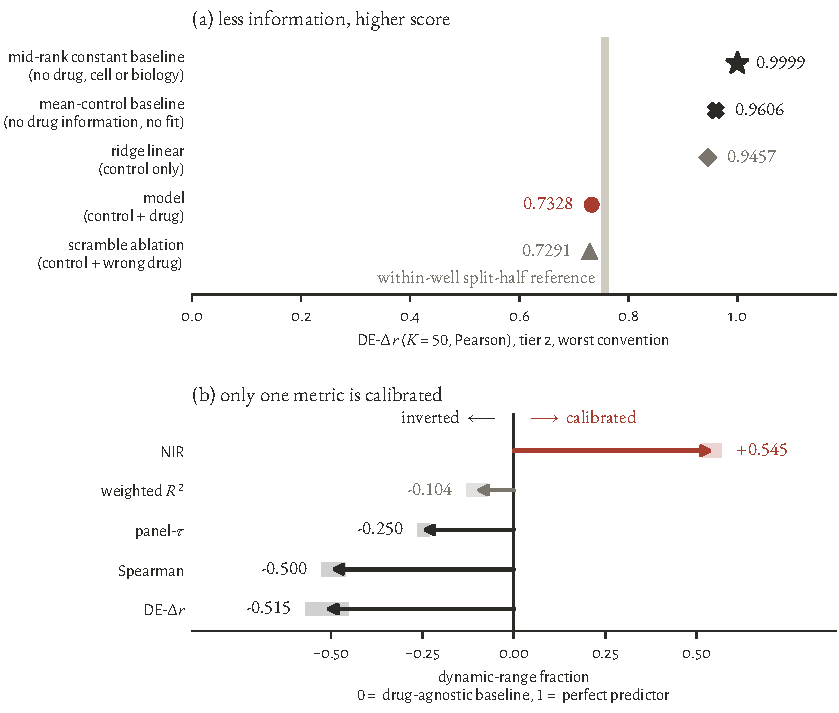
\includegraphics{fig-calibration}
\caption[A zero-information predictor outscores the model]{\captiontitle{A predictor
carrying nothing about drug, cell or biology scores the field's standard metric
above both the within-well reference and the model, and of five metrics only
$\NIR$ grades in the direction its name implies.} (a) $\DEdr$, $K = 50$,
Pearson, tier 2 unseen drugs, \texttt{worst} convention, $n = 400$ conditions;
the axis runs from $0$ and is not truncated. The grey band marks the within-well
split-half precision reference at $0.76$, the two-real-cell positive control of
\cref{tab:de-artifact}: two halves of the same well, a precision figure and not
a biological replicate. Its width is a drawing device, not an interval, and the
arm marks are bare --- the source carries a normal-approximation interval over
conditions, and this document draws only the clustered bootstrap, so nothing is
drawn rather than an interval of another kind. (b) $\DRF$ for the five metrics
of \cref{tab:drf}, the same-plate arm only: $586$ drugs over $44$
cell-line$\times$plate groups spanning $27$ cell lines, the pale block at each
arrowhead the $95\%$ percentile bootstrap interval clustered on cell line
quoted there.}
\label{fig:calibration}
\end{fullwidth}
\end{figure}

\paragraph{What this replicates, and where it does not} The methodological core
of Miller et al.\ replicates, and this audit sharpens it. Metric choice
dominates, and the
control-referenced correlation they flag is the worst performer in both arms
($\DEdr$, $-0.686$ across plates and $-0.515$ within). Their calibrated set does
not transfer intact. \texttt{weighted\_r2}, this project's counterpart of the
weighted $R^2\Delta$~\cite{mejia} they endorse, is negative in both audited
arms, though closest to zero and sign-tracking cell count, so it carries no
directional claim; the inversions of $\paneltau$ and \texttt{spearman\_expr}
belong to neither calibrated set. Their endorsed $\NIR$ does survive. Being
rank-based is not what protects it; refusing to score anything the generic
response can supply is.

\paragraph{Adopting the instrument is also a defence} Miller et al.\ conclude
that under calibrated metrics deep models outperform uninformative baselines;
\cref{sec:res-blind} finds ours at chance on that metric, in the decoded
representation the verdict deploys and not in the one the audit
graded.\seealso{\cref{sec:lit-dispute} sets out the dispute this audit enters.}
Genetic against drug perturbation and a discriminative against a generative
model are candidate explanations; \cref{sec:res-lookup} supplies a third.
Adopting their metric also puts the verdict beyond the objections their own
paper raises.

\paragraph{One declared exception on the intervals} $\DRF$ is a ratio of means;
the two-way estimator used everywhere else here is written for a
mean.\bench{two-way cluster-robust intervals on every
mean}{\cref{sec:methods-data}} Both $\DRF$ intervals are therefore
\emph{one-way} percentile cluster bootstraps that resample whole cell lines and
recompute the ratio inside each draw, respecting the cell-line dependence and
ignoring the crossed well dimension, so they are narrower than fully crossed
intervals. The separation they grade is far too large for that to change the
sign, but the caveat belongs beside the number.

\paragraph{Two questions about the instrument remain, and they differ} The first
is whether the conditions are empirically discriminable at the tested budget. A
spike-in forced choice answers it. Within a plate, a reference pseudobulk from
drug A's cells must be scored closer to a disjoint sample of A's own cells than
to drug B's, chance $0.50$, with contamination of B by A titrating the
difficulty. At zero contamination three of the six metrics run on it
separate the two populations essentially perfectly ($\paneltau = 1.000$,
$\DEdr = 0.995$, top-$n$ $\tau = 0.987$, plate held constant); at full
contamination those same three return $0.501$--$0.502$. The whole-profile
similarities are much weaker even at zero contamination, cosine $0.740$,
Spearman $0.680$, cosine on the shift $0.620$, which matters because a
whole-profile similarity is what $\NIR$ uses here. Split-half retrieval
establishes discriminability, not predictability from untreated input, so
discriminability is not the sole bottleneck at this budget.

The spike-in cannot answer the second question, whether $\NIR$ registers a true
positive, since $\NIR$ was not among the metrics run on it. The evidence is the
$\DRF$ audit's own positive control. Under $\NIR$ on measured expression the
interpolated
duplicate scores $0.802$ against the drug-agnostic mean's $0.457$ across plates,
and $0.668$ against $0.272$ within plate; in the residual frame a split-half
replicate reaches $0.854$ against negatives at $0.501$--$0.506$. None of those is
the reference the verdict is measured against. That reference is the within-well
split-half precision estimate recomputed on the tier-2 within-plate benchmark,
where it sits above chance but not far above it; that, and not $1.0$, is the bar
\cref{sec:res-blind} states the model against.

\begin{scopelimit}[carried into \cref{sec:res-blind} and the rest of the chapter]
The audit licenses $\NIR$ and nothing else. $\paneltau$ is inverted in both
audited arms, so no absolute claim rests on it and no ordering read off it counts
as evidence of skill; an inverted metric preserves neither. Where $\DEdr$
appears later it is only as a paired comparison of two arms on one scale, never
as an absolute score. And a metric is not calibrated by having a relative
calibrated. What is graded here is a negated Euclidean distance on measured
pseudobulk expression, the second row of \cref{tab:sigma}, and the residual
frame's cosine similarity in its own frame, each against its own controls. The
\texttt{nir\_expr} of the blindness verdict is that distance read on decoded
pseudobulk, the first row, with controls of its own but no $\DRF$ of its own, so
it stands on the assumption above. A third $\sigma$ would need its own audit.
\end{scopelimit}

\begin{claim}
This audit grades five candidates, and $\NIR$ is the only
one with a positive $\DRF$ (\ci{+0.635}{+0.604}{+0.663} on a one-way cluster
bootstrap over the $25$ cell lines, the declared exception to this chapter's
two-way rule, Holm $p = 0.002$; \ci{+0.545}{+0.516}{+0.569} over $27$ cell lines
with same-plate partners, Holm $p = 0.002$), and the other four are negative with
intervals excluding zero in both audited arms. Three of them ($\paneltau$,
\texttt{spearman\_expr} and $\DEdr$) are inverted rather than merely
uninformative, each ranking the drug-agnostic baseline above the positive
control; \texttt{weighted\_r2} sits closest to zero and its sign tracks cell
count, so no directional claim is made for it. The saturating predictor is not a
curiosity. It carries no information about drug, cell or biology and scores
$\DEdr = 0.9999$ in rank space, above the two-real-cell positive control of
$0.76$ and above the model's $0.73$. Under $\NIR$ on measured expression the positive control is retrieved well clear of
the negative ($0.802$ against $0.457$ across plates, $0.668$ against $0.272$
within), so the instrument registers a true positive. Every drug-use claim in
the rest of this chapter that rests on a continuous prediction score is
therefore made on $\NIR$, in the audited construction where the audit reaches
and in the decoded one that inherits its licence where it does not; $\DEdr$
appears below only where two arms are compared with each other on the same
scale, never as an absolute score of the model's drug use. The remaining instruments (forced-choice grading,
output invariance, and the logit-space activation tests of
\cref{sec:res-mechanism}) are deliberately on scales of their own, each with a
fixed chance value or a paired control.
\end{claim}

% ===========================================================================
% Beat 2.
% ===========================================================================

\beatsection{E}{2}{In the expression frame, the model is drug-blind}{sec:res-blind}
\label{sec:methods-controls}   % legacy anchor, so v1 cross-references resolve


\begin{question}[2]
With a properly calibrated metric in hand, the investigation can ask the
question it exists to answer. Does the model use the drug at all to make predictions? Four
instruments answer it, and each exists because one specific objection would
otherwise be fatal.
\end{question}

\noindent
The answer is no, and reaching it takes more than a scoreboard. With the metric
calibrated, the model can finally be scored on the tiers, and two readings follow
that look nothing alike and settle nothing on their own.

Within plate on tier 2 ($n = \num{606}$) the model scores $0.498$ against a
within-well split-half precision reference of $0.576$.\bench{one estimator,
seven settings}{\cref{tab:ceilings}} The gap is narrow, but so is the scale: the
reference itself stands only a little above chance, and the model sits at chance
inside it, matched by predictors that know nothing about the drug --- a
drug-agnostic linear map at $0.500$ and a control-copy at $0.504$, against the
global mean's $0.180$. That average also hides a split. Binning the same $\num{606}$
conditions by their own reference gives $296$ on which the reference falls
\emph{below} chance, at $0.287$, where not even a second sample of the same well
scores above chance; $106$ marginal; and $204$ identifiable, whose reference
clears the pre-set $0.80$ bar. On that last third the model looks far better and
discriminates well above chance, reaching $0.768$. A control-copy carrying no
drug information whatsoever reaches $0.766$.

Neither reading is causal, and that is the whole difficulty. A model scoring at
chance might be ignoring the drug, or reading it and failing to turn it into
anything; a model scoring $0.768$ where a drug-blind predictor scores $0.766$
might be adding nothing, or adding something too small for the metric to resolve.
The two readings even point opposite ways, one suggesting the model has learned
nothing and the other that it has learned a good deal, and both are consistent
with the drug token never being consulted. No comparison of scores can separate
these, because no comparison of scores intervenes on anything. What settles it is
an experiment in which the drug changes and nothing else does.

\paragraph{Four instruments, and each closes a different objection} The four are
not four attempts at one measurement. The second is the experiment the previous
paragraph asked for, and the others exist because that experiment is still scored
by something, and whatever scores it could be blamed for the result. Each
successive instrument removes another part of the apparatus from the argument.

The first is the benchmark itself, run \emph{within plate}. Drug and plate are
partially confounded by the atlas's design, so a comparison set free to span
plates lets a batch effect stand in for drug identity and inflates every arm at
once. Restricting the set to a single plate removes that channel before anything
else is asked.

The second is the scramble ablation, and it is the only manipulation among the
four. The control cell is held fixed and only the drug name and mechanism in the
prompt are replaced, by a different drug on the same plate; everything the model
sees apart from the drug is unchanged. A gap between the two generations is
caused by the drug or by nothing, which is what no comparison of scores could
establish. Here the partner is drawn at random, and that carries a known risk: a
swap to a drug with a similar true response makes an unchanged output correct
rather than blind, which biases the test toward finding nothing. A swap-distance
sweep bins (drug, swap) pairs by the response distance between the real and the
swapped-in drug, turning the single test into a curve, and
\cref{sec:res-generalisation} returns to the question with partners stratified by
residual cosine, where a neutral null can be identified rather than assumed.

The third is forced-choice grading. A prediction is scored against its own
condition's truth and against another drug's truth from the same comparison set,
and what is recorded is how often its own wins. 

The fourth is output invariance, and it touches no truth at all. It asks only
whether changing the drug token changes the generated text, comparing generations
against other generations from the same fixed control cell. No similarity
function against a ground truth, no comparison set and no decode enters it, so no
scoring choice can confound it. It is the least informative of the four and the
least confoundable, and those are the same property.

Taken together they share a model and little else. The first can be defeated by
batch leakage, the second by a badly chosen swap partner, the third by a
degenerate comparison set, the fourth by nothing except the model genuinely
ignoring the drug --- and it is that lack of a common failure mode, rather than
any one of them, that carries the verdict.

\paragraph{One measurement rule comes first} Drug and plate are partially
confounded by the atlas's design
(\cref{sec:methods-data}),\framecue{\Eframe}{all four instruments are scored in
the expression frame} so grouping by cell line alone lets the batch effect
stand in for drug identity. A drug-agnostic mean baseline, containing no drug
information whatsoever, scores $0.399$ when the comparison set may span plates
against $0.161$ when it may not, and the precision reference falls from $0.625$
to $0.575$ alongside it, the batch
effect having inflated that too.\seealso{\cref{tab:plateleak} is the leak
audit, a wider run than the benchmark} That is plate leakage, measured and not
assumed. Being wider, its within-plate figures sit slightly off the ones above;
what it licenses is the rule, not a substitute set of scores.

\begin{scopelimit}[carried into every discrimination result in this chapter]
Every discrimination instrument gained a \texttt{--same\_plate\_only} mode and
every discrimination result in this chapter was re-run within plate, except
where a departure from that rule is named at the point of use, as with the
swap-distance sweep that answers the fourth objection below, whose swap partners
were not plate-restricted (\cref{sec:app-sweep}), and the residual-frame scores
of \cref{sec:methods-residual}, whose comparison set is grouped by cell line and
whose justification is given there. A third departure is the identifiability
curve in \cref{tab:ceilings}: it is cross-plate because no within-plate sweep
reaches the cell budgets it reports, the plate-matched version stopping at
twenty cells per condition, and it is computed on raw pseudobulk rather than on
the decoded expression the rest of that table uses. It is therefore read as a
statement about aggregation and never set beside the within-plate references
above it. Conclusions are unchanged; some magnitudes shrink.
\end{scopelimit}

\paragraph{The central manipulation is the scramble ablation} The prompt is left
byte-identical except that the drug name and mechanism are replaced by another
drug's, the control cell and the scoring truth unchanged. Control- and batch-derived leakage therefore cancels in
the scramble gap $\gap = \NIR_{\textrm{model}} - \NIR_{\textrm{scramble}}$, the
only difference in this chapter whose leakage cancels by construction. It does
not displace the drug-agnostic comparisons above and below, which rest on the
within-plate rule instead.

Where that ablation is applied is a choice, and this chapter makes the hard one
first. Every scramble in this section is scored on \texttt{tier2}, held-out
drugs the checkpoint never saw in training, and the substituted partner is drawn
from that same held-out tier --- so the model is asked to distinguish two drugs
it knows nothing about. Nothing here is measured on trained conditions; the
\texttt{tier1} arm of these runs returned no scoreable conditions at all, since
$\NIR$ needs a per-condition pseudobulk and that tier averages roughly two cells
per condition. \Cref{sec:res-encoding} later runs the easier version of the same
manipulation, scoring a model on conditions it did train on, where a drug-blind
model has memorisation to fall back on and any real drug sensitivity has its
best chance of showing. That the expression-frame arms fail here, on the harder
test, is what this section establishes; that the easier test does not rescue
them is \cref{sec:res-epsilon}'s result, and that one target construction does
separate under it is \cref{sec:res-encoding}'s.

% PLACEMENT ONLY. The float was anchored six paragraphs lower (just before "The
% third instrument"), which is where its [htbp] first became satisfiable -- the
% top of the NEXT page -- and that page then had no room left for
% \cref{tab:blind}, which was pushed a further page past the sentence that
% introduces it (measured: anchor p35, caption p37). Anchoring the figure at the
% paragraph it actually depicts, the scramble ablation itself, is earlier in the
% flow, so the figure takes the top slot one page sooner and the table follows on
% the page after its own anchor. Nothing about the figure or its caption changes.
%
% The paragraph above now carries the \cref, so the anchor is explicit and not
% merely positional. Its second sentence lost the restatement "Both arms share
% the same control cell, so ..." because the figure now sets that clause on one
% unbroken line beneath the two arms; the inference is carried by "therefore"
% off "the control cell ... unchanged" in the sentence before it. No claim,
% hedge or magnitude changed, and the paragraph is one line shorter than it was.
%
% \input, not \includegraphics: figs/fig-scramble.tex is TikZ and carries its
% own float, caption and \label. \input resolves against the main-document
% directory, so this is thesis_v2/figs/, NOT the read-only ../thesis/figs/ that
% \graphicspath adds for raster/PDF assets only.
\begin{figure}[htbp]
% MARGINALIA (06-figures.md): fits the text column; caption in the margin.
\begin{lrbox}{\tvfb}%
  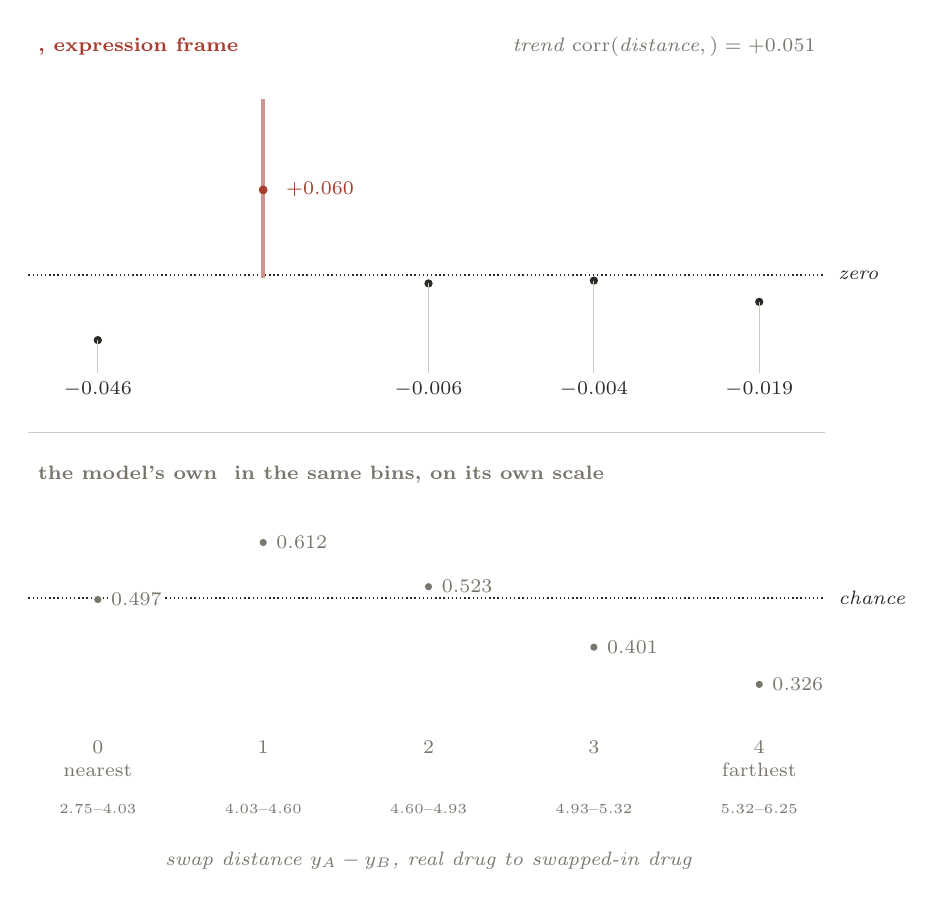
\begin{tikzpicture}[x=21mm, y=1mm, font=\small]
    \def\ur{180}                     % upper strip, mm per unit of the gap
    \def\lz{-52}\def\ls{63}          % lower strip, origin and mm per unit
    \def\lchance{\lz+(0.5-0.326)*\ls}% $\NIR = 0.50$ on the lower strip
    % Four of the five gaps sit within a few thousandths of zero. The dot stays at
    % its true height and the label drops straight down to one aligned row, so the
    % series reads as the flat line it is rather than as five scattered labels.
    \newcommand{\gapdot}[2]{%
      \fill[ink] (#1,{#2*\ur}) circle (1.5pt);
      \draw[rulegrey, line width=0.3pt] (#1,{#2*\ur}) -- (#1,-12.4);
      \node[anchor=north, font=\scriptsize, text=ink] at (#1,-12.4) {$#2$};}
    \newcommand{\nirdot}[2]{%
      \fill[quietink] (#1,{\lz+(#2-0.326)*\ls}) circle (1.3pt);
      \node[anchor=west, font=\scriptsize, text=quietink, fill=white, inner sep=1pt]
        at (#1+0.06,{\lz+(#2-0.326)*\ls}) {$#2$};}
  
    % === upper strip, the scramble gap ========================================
    \node[anchor=west, font=\scriptsize\bfseries, text=accent]
      at (-0.42,29) {$\gap$, expression frame};
    \node[anchor=east, font=\scriptsize\itshape, text=quietink]
      at (4.40,29) {trend $\mathrm{corr}(\textrm{distance},\gap) = +0.051$};
    \draw[ink, line width=0.5pt, densely dotted] (-0.42,0) -- (4.40,0);
    \node[anchor=west, font=\scriptsize\itshape, text=ink] at (4.42,0) {zero};
  
    % the one bin for which an interval is quoted, drawn as an interval
    \draw[accent!55, line width=1.6pt] (1,{-0.002*\ur}) -- (1,{0.124*\ur});
    \fill[accent] (1,{0.060*\ur}) circle (1.6pt);
    \node[anchor=west, font=\scriptsize, text=accent]
      at (1.08,{0.060*\ur}) {$+0.060$};
  
    \gapdot{0}{-0.046}
    \gapdot{2}{-0.006}
    \gapdot{3}{-0.004}
    \gapdot{4}{-0.019}
  
    % === the divider IS the argument: two quantities, two scales, one x =======
    \draw[rulegrey, line width=0.4pt] (-0.42,-20) -- (4.40,-20);
  
    % === lower strip, the model's own score, which drifts =====================
    \node[anchor=north west, font=\scriptsize\bfseries, text=quietink]
      at (-0.42,-23) {the model's own $\NIR$ in the same bins, on its own scale};
    \draw[ink, line width=0.5pt, densely dotted]
      (-0.42,{\lchance}) -- (4.40,{\lchance});
    \node[anchor=west, font=\scriptsize\itshape, text=ink]
      at (4.42,{\lchance}) {chance};
    \nirdot{0}{0.497}
    \nirdot{1}{0.612}
    \nirdot{2}{0.523}
    \nirdot{3}{0.401}
    \nirdot{4}{0.326}
  
    % === the one axis the two strips share ====================================
    \foreach \i/\lab/\rng in {0/nearest/{2.75--4.03}, 1/{}/{4.03--4.60},
                              2/{}/{4.60--4.93}, 3/{}/{4.93--5.32},
                              4/farthest/{5.32--6.25}}{
      \node[anchor=north, font=\scriptsize, text=quietink, align=center]
        at (\i,-58) {\i\\\lab};
      \node[anchor=north, font=\tiny, text=quietink] at (\i,-66) {\rng};}
    \node[anchor=north, font=\scriptsize\itshape, text=quietink]
      at (2,-72) {swap distance $\lVert y_A - y_B \rVert$, real drug to swapped-in drug};
  \end{tikzpicture}
  %
\end{lrbox}
\sidecap[The scramble gap does not grow with swap distance]{figure}{\captiontitle{Naming a
  drug whose response is far from the truth damages the prediction no more than
  naming a near neighbour.} Results taken in the Tier 2. Upper strip, the scramble gap across five bins of swap
  distance. A real dissimilarity effect would climb from left to right and peak at
  the farthest bin; instead the correlation between distance and gap is $+0.051$,
  and the only bin whose interval is quoted, \ci{+0.060}{-0.002}{+0.124}, is the
  second of five. Lower strip, the model's own $\NIR$ in those same bins, which
  does fall overall, though not monotonically, because drugs far from everything
  populate the far bins. The two strips are different quantities on different
  scales, and $\gap$ uses the same drug on both arms, so that drift cancels out of
  it. Non-canonical: \texttt{max\_new\_tokens=1200}, $n = 40$ per bin, which
  excludes a large dissimilarity effect without establishing a null.\label{fig:sweepbins}}
  
  
\end{figure}

\paragraph{Two constraints on the swap partner} The partner must be a different
drug. Allowing the same drug at another dose or plate substitutes the drug for
itself, an unchanged prediction is then correct and not blind, and the contamination
concentrates in the most similar stratum. It must also be on the same plate,
since residuals retain plate structure and a cross-plate partner would differ in
batch as well as in drug.

A scramble that swaps in a drug with a similar true response is a weak test, and
that risk is structural here. In full-profile space the mechanism annotation is
close to uninformative about transcriptional response. Same-mechanism drugs in
Tahoe are just over two per cent closer to each other than arbitrary pairs
are.\seealso{\cref{sec:res-encoding} quotes the distances behind that statement}
Hence conditioning on mechanism fails to move $\DEdr$ in the grouping ladder of
\cref{sec:res-lookup}, and a partner of different mechanism cannot be relied on
for a different response. Mechanism does carry signal in the residual frame
(\cref{sec:res-scope}); in full-profile space the generic response swamps it, a
frame difference and not a contradiction.

Two remedies are used, one here and one later. The first turns the single test
into a curve. Within a (cell line, plate) group, each drug's cells are split in
half and the distance between two drugs is taken between their half-sample truth
pseudobulks, $\lVert y_A - y_B \rVert$. Because both profiles sit against the
same plate-matched control, that distance is the same whether it is measured on
profiles or on shifts, and it is exactly the distance $\NIR$ already uses to rank
one condition's truth against another's. The sweep therefore inherits the
benchmark's own geometry rather than importing a notion of similarity from
elsewhere, and the axis is fixed before any generation: it is a property of the
atlas, not of the model.

Partners are drawn to span the quantiles of that distance from $A$, so each real
drug contributes swaps from across its whole available range instead of one
partner of unknown similarity. Every swap rebuilds $A$'s prompt with $B$'s name
and mechanism, leaves the control cell and the rest of the prompt intact, and
scores the generation against \emph{$A$'s} truth. The target never moves; only
the label in the prompt does. Pooling the pairs and binning them by distance
gives five bins running from nearest to farthest
(\cref{fig:sweepbins}, \cref{sec:app-sweep}), and the gap is aggregated inside
each bin with intervals clustered on cell line.

What makes the curve worth reading is that each outcome was given its meaning
before the run. A gap rising with distance would say the model does discriminate
dissimilar drugs and that the flat aggregate had been diluted by near-twin swaps
--- a correction to the claim, not a confirmation of it. A gap that stays flat
into the far tail says the blindness holds at the hardest setting the plate
affords, where the swapped-in drug's real response is as unlike the truth as the
data allows.

\paragraph{The third instrument is forced-choice grading} A prediction is scored
against its own condition's truth and against another drug's truth from the same
comparison set, recording how often its own wins. Chance is $0.50$ by
construction, and the precision reference lands between $0.67$ and $0.83$
depending on cells per condition.

\paragraph{The fourth is output invariance} It asks whether the drug token
changes the generated text at all, without reference to any truth. It is run at
$3800$ tokens, the longest budget in the chapter, because
truncation would cut the comparison
itself.\seealso{\cref{sec:methods-data} records the four generation budgets} For
a fixed control cell it compares
% \resizebox, not a reflow: the two \underbrace labels are the width, and both
% are wanted on one line so the subtraction reads as one sentence. Natural
% width is 165.6mm against the 142mm block (67.15pt over), so this sets at
% about 0.86. Nothing here is body text.
\begin{equation}
\resizebox{\linewidth}{!}{$\displaystyle
 \textrm{invariance gap} \;=\;
 \underbrace{\overline{\textrm{sim}}(\textrm{same prompt, resampled})}%
   _{\textrm{sampling noise alone}}
 \;-\; \underbrace{\overline{\textrm{sim}}(\textrm{prompts differing in the
   drug})}_{\textrm{noise plus any drug effect}},
$}
\end{equation}
with similarity as top-$100$ Kendall $\tau$ and as Jaccard overlap, over $8$
contexts $\times$ $12$ drugs at temperature $0.8$. It is the least informative
of the four and the least confoundable.

\begin{table}[htbp]
% MARGINALIA: full width; caption above at the text width, the one note below.
% No highlight: four instruments agreeing is not one cell.
\caption{\captiontitle{Four independent instruments agree, and the two that return
intervals bound the drug's effect instead of merely covering zero.} Near-ceiling
$\DEdr$ is achieved identically with a wrong-mechanism drug, so that score is
drug-independent.}
\label{tab:blind}
% Column 3 was `l', then a weighted X: at an earlier, narrower measure its
% natural width plus columns 1--2 left the last column too narrow for the
% single unbreakable word "indistinguishable", which ran 43.91pt past the
% fullwidth block, and the X let the \ci intervals break after the estimate.
% Column 3 is `l' again so no \ci ever breaks mid-cell; at the 182mm measure
% the first three columns' natural widths leave the Reading column, a Y, about
% 44mm, so "indistinguishable" fits.
\begin{fullwidth}
\begin{threeparttable}
\begin{tabularx}{\linewidth}{@{}l l l Y@{}}
\thead{Instrument} & \thead{Quantity} & \thead{Value} & \thead{Reading} \\
\midrule
Forced-choice grading & own-truth win rate
  & $0.48$ ($\approx$ scramble; reference 0.67--0.83) & chance \\
\addlinespace[10pt]
Output invariance & invariance gap, top-$100$ $\tau$ & \ci{0.000}{-0.019}{+0.016}
  & bounded, $\leq 0.016$ \\
 & invariance gap, Jaccard & \ci{+0.000}{-0.008}{+0.008}
  & bounded, $\leq 0.008$ \\
\addlinespace[10pt]
Scramble, tier 1 & $\DEdr$ & $0.740$ real vs $0.739$ scrambled
  & indistinguishable \\
Scramble, tier 2 & $\DEdr$ & $0.733$ real vs $0.729$ scrambled
  & indistinguishable \\
Scramble (identifiable subset) & $\gap$ ($\NIR$) & \ci{+0.014}{-0.016}{+0.042}
  & bounded, $\leq +0.042$ \\
\end{tabularx}
\begin{tablenotes}[flushleft]
\item The two $\DEdr$ rows are paired comparisons on one scale, the only use
\cref{sec:res-metrics} licenses for that metric.
\end{tablenotes}
\end{threeparttable}
\end{fullwidth}
\end{table}

% PLACEMENT ONLY. This is one of the three survivors the \paragraph orphan patch
% in preamble.tex section 4 records: the global reservation is
% 3\baselineskip, which this head cleared with 2.3 lines to spare and then set
% itself plus exactly two lines at the foot of the page. 5 lines is head plus
% four, which the page cannot fake.
\needspace{5\baselineskip}%
\paragraph{An interval that covers zero earns its keep by what it excludes} Not
by the word \emph{null}. Two predictions from a byte-identical prompt agree at
$\tau = 0.198$, so the invariance interval caps any drug-driven divergence at
roughly a twelfth of that agreement, and the Jaccard version is tighter still,
\ci{+0.000}{-0.008}{+0.008}. On the identifiable stratum the scramble gap of
\ci{+0.014}{-0.016}{+0.042} runs against the $0.170$ separating the model's
$0.768$ from that stratum's $0.938$ reference; at the very top of the interval,
naming the right drug would buy a quarter of what is there to be bought, and the
point estimate puts it at $8\%$ of that. Neither figure shows the effect is
zero, and no experiment here could. Both put it far below the headroom these
conditions leave.


\begin{figure}[htbp]
\begin{fullwidth}
  \raggedright
  % drawn at 142mm by thesis_v2/figs/difficulty.py; no width= key, so it is placed
  % at scale 1.0 and its type prints at the point sizes it was set in.
  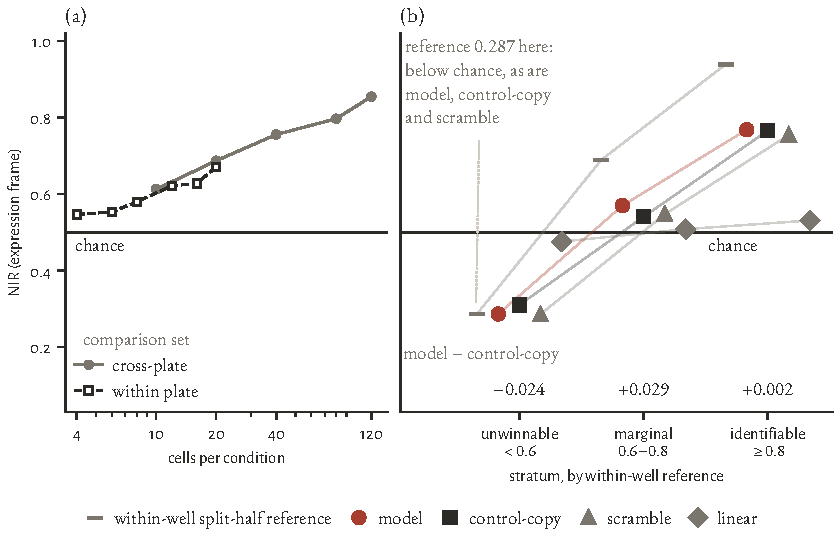
\includegraphics{fig-difficulty}
  \caption[Difficulty structure and the stratum ladder]{\captiontitle{Conditions are
  more empirically discriminable at the tested pseudobulk budget where the
  precision reference is high, and precisely there, a predictor containing no drug
  information matches the model.} Both panels are $\NIR$ in the expression frame,
  on one shared axis. (a) The within-well split-half precision reference against
  cells per condition, for two comparison sets: cross-plate, and within plate. (b)
  The same reference used to bin conditions, five arms per stratum, $n = 296$
  unwinnable, $106$ marginal, $204$ identifiable. On the unwinnable stratum the
  reference itself is $0.287$, below chance, as are the model, control-copy and
  scramble marks. On the identifiable stratum the model reaches $0.768$ and a
  control-copy baseline $0.766$, paired contrast \ci{+0.002}{-0.026}{+0.028},
  clustered over cell lines. Plotting the model alone would suggest it does better
  on higher-reference drugs. The arm marks are bare: the source carries no
  interval for a stratum mean, and this document draws only the clustered
  bootstrap, so nothing is drawn rather than an interval of another kind.}
  \label{fig:difficulty}
\end{fullwidth}
\end{figure}
  \paragraph{Four ways the verdict could be an artefact} Each is a way the result
  could be about the apparatus rather than about the model, and each is settled by
  a measurement rather than by argument.
  
  \emph{That there is nothing to learn.} A ladder of mean-shift baselines, each
  predicting the average shift of a progressively narrower group, says
  otherwise.\seealso{\cref{sec:res-lookup} gives the ladder} On tier 2 the global
  mean scores $0.056$ and conditioning on cell line raises it about
  two-and-a-half-fold to $0.142$, so the atlas carries real structure. What it does
  not carry is structure the drug label reaches: mechanism leaves the global figure
  untouched at $0.052$, and mechanism together with cell line does no better than
  cell line alone ($0.120$ against $0.142$). There is something to know, and the
  variable that knows it is the cellular context.
  
  \emph{That the benchmark is too weak to say anything.} Barely half the atlas
  clears the pre-set identifiability bar (\cref{tab:scale}), so the verdict is
  re-scored where the wells are demonstrably adequate. It does not survive the
  move. On that stratum the model appears to beat the linear baseline, $0.768$
  against $0.531$, and then a control-copy carrying no drug information reaches
  $0.766$ on the same conditions; the paired contrast is
  \ci{+0.002}{-0.026}{+0.028} and the leak-immune $\gap$ stays bounded as above.
  
  That control-copy carries a second finding, and it is easy to walk past. Across
  the three strata its score tracks the reference almost step for step
  (\cref{fig:difficulty}, panel b): $0.310$ against a reference of $0.287$ where
  the reference is lowest, $0.540$ against $0.689$ on the marginal stratum, $0.766$
  against $0.938$ on the identifiable one. A predictor that knows nothing about any
  drug does best exactly where the ranking problem is easiest. So what makes a
  condition identifiable is largely what makes its untreated cells distinctive
  among their plate-mates, and the distance from the model to a high reference is
  not all room that better drug modelling would fill. The reference does rise with
  aggregation (\cref{fig:difficulty}, panel a: $0.61$ at $10$ cells, $0.76$ at
  $40$, $0.85$ at $120$); what the strata add is that most of the ranking can be
  done without the drug at all.
  
  \emph{That the encoding discards the drug.} A cell sentence keeps the rank order
  of genes and throws away expression magnitude, so if the drug lived in the
  magnitudes the following sections would be attacking the wrong object. This needs
  no model to test: ask whether true expression discriminates drugs better than
  rank does. It does not. At single-cell resolution, cosine, Pearson and Spearman
  similarities on true normalised expression all sit within $0.04$ of chance
  (\ci{0.529\textrm{--}0.531}{0.515}{0.543}), the same near-chance regime as rank.
  What recovers the signal is aggregation: at fifteen cells the control-referenced
  shift cosine reaches \ci{0.793}{0.775}{0.809}. The re-encoding of
  \cref{sec:res-encoding} will therefore not be a restoration of magnitudes; it
  keeps rank throughout and changes only what is ranked. The same measurement also
  bounds what a single cell can deliver, since the single-cell same-drug against
  different-drug gap is only \ci{+0.006}{+0.003}{+0.008}: these instruments do not
  resolve drug identity from one observed cell at this sequencing depth and
  $946$-gene panel.
  
  \emph{That the scramble swaps in near-twins.} The swap-distance sweep bounds this
  rather than settling it. It sits outside the within-plate rule, an earlier run at
  \texttt{max\_new\_tokens=1200} on the unseen-drug tier of a different evaluation
  set, with swap partners not plate-restricted and $n = 40$ per bin --- wide enough
  to exclude a large effect, not to establish a null (\cref{sec:app-sweep}). No
  distance bin has an interval excluding zero. The far tail reads $-0.019$ across a
  $2.3\times$ spread in swap distance with a trend correlation of $+0.051$, so a
  large dissimilarity effect is excluded for the expression-frame model and a small
  one is left open.
  
  \paragraph{What none of the four can see} All four watch the output. They
  establish that the generated text does not move when the drug does, and that is
  the strongest behavioural statement available. It is also silent on why. A model
  that never encodes the drug and a model that encodes it and uses it incorrectly
  produce the same flat instruments, and no experiment that only reads generations
  can separate them. The ladder above already hints at where to look, since the
  asymmetry it finds between cellular context and drug class is one the activations
  turn out to repeat. \Cref{sec:methods-probe} therefore stops asking what the
  model emits and starts asking what it holds.

    \paragraph{A fifth reading of the same sweep, with no comparator in it} 
    The four
  instruments above each contrast the model against something --- a baseline, a
  control-copy, a scrambled prompt --- and each is only as good as the thing it is
  set against. The swap-distance sweep supports one further reading that contrasts
  nothing. Its partners were drawn to span the distance quantiles, five per
  condition, so within a single condition the same model answers the same question
  five times with a differently wrong drug named each time. Write $y_{ik}$ for the
  $\NIR$ of condition $i$'s $k$th scrambled prompt and $x_{ik}$ for the
  \emph{negated} Euclidean distance between that condition's truth and the truth of
  the drug substituted into it --- negated so that $x$ rises with similarity, as
  the partner cosine does everywhere else in this thesis, and one predicted sign
  serves every version of the test. Then
  \begin{equation}
   y_{ik} \;=\; \alpha_i \;+\; \beta\,x_{ik} \;+\; \varepsilon_{ik},
   \qquad k = 1,\dots,5,
  \end{equation}
  with one intercept $\alpha_i$ per condition. The target-drug prompt is never a
  point on this line, so nothing is measured against a chosen baseline, and
  $\beta = 0$ is the null by construction: a model that ignores the name emits the
  same distribution whichever drug is substituted, putting its five points at one
  height whatever their similarities happen to be. Prompt sensitivity predicts
  $\beta > 0$, the score rising as the substituted drug's real response moves
  closer to the target's.

  Which intercepts are fitted decides the answer. A single pooled intercept draws
  one line through all $200$ points at once, so conditions are compared with each
  other as much as with themselves, and fitted that way the slope is $+0.0986$
  $[+0.0180, +0.1792]$ clustered on drug --- a clear effect, and not a real one. A
  condition whose drug is unlike anything else on its plate has distant partners
  \emph{and} an unusual truth that any prompt will struggle to rank, so the line
  bends without a name having been read. Giving each condition its own intercept
  removes that comparison and leaves only what varies inside a condition: one
  model, one target, five differently wrong drugs. Almost the whole effect is in
  the part that discards --- the between-condition slope is $+0.1563$ against a
  within-condition slope of $+0.0055$, $[-0.0472, +0.0582]$ clustered on drug and
  $[-0.0484, +0.0594]$ on cell line, over $200$ prompts across $40$ conditions.
  The tighter interval excludes the pooled estimate it replaces. Compared with
  itself, no condition's score moves with how unlike the substituted drug is.

  What this adds is not more of the same evidence. The scramble is a paired
  intervention --- one condition, one thing changed --- and is confound-free by
  construction, but it needs a comparator, and \cref{sec:res-generalisation} shows
  how much of a gap the choice of comparator can carry. This regression needs none.
  What it gives up in exchange is what it can license: every point in it is a
  \emph{wrong} prompt, so it can show only whether the model tells wrong answers
  apart, never whether it produces a right one. A model could pass it and predict
  nothing. Here that trade costs nothing, because the model does not pass it.

\begin{claim}
The model is at chance overall ($0.498$ against a $0.576$ within-well split-half
precision reference), matched on the identifiable stratum by a
zero-drug-information control-copy ($0.768$ against $0.766$, paired contrast
\ci{+0.002}{-0.026}{+0.028}), and no more moved by a maximally dissimilar swap
than by a similar one in the single-cell column of a non-canonical
\texttt{max\_new\_tokens=1200} sweep outside the within-plate rule
(\cref{sec:app-sweep}). 
\end{claim}

% ===========================================================================
% 04b-representation.tex -- beats 3-4. The expression frame, read in the weights.
% Source: thesis/Sections/Investigation-v4.tex 1052-1545.
% Every number, interval, n and conclusion is verbatim from v1.
%
% Consistency pass: the section now opens by naming the third question of
% \cref{sec:intro-map} and stating its answer -- identity written into the
% activations, barely consulted by generation -- before the instruments, so a
% reader arriving from the introduction finds what was promised. The stratum
% paragraph and its \scopelimit are adjacent again, since the scope limit is
% about that stratum's reference. "Step three, the removal gate" was a \defn
% box between three \paragraph steps; it is now the paragraph it always was,
% merged with the gate result that followed it. Vocabulary: "output" as a noun
% for the prediction, "compound", and bare "signature" are gone; "shift" is
% reserved for treated minus control, so the logsumexp constant is an offset.
% "Energy" is gone as well, and it went two ways because it named two different
% things. The $\approx 99.5\%$ that a full-stream control puts outside the slab
% is a projection share of a squared Euclidean norm, $1 - 10/2048$ for ten
% intervention directions in $2048$, so it now reads "squared norm", in the
% sense fixed by the norm entry in the symbols list of 00-HowToRead.tex. It is
% not the residual/generic decomposition of shared/inference.py, whose
% docstring calls itself a variance decomposition and is wrong to: nothing is
% centred there either. The "strong-programme energy" of the paragraph on where
% ablation stops named no computed quantity at all, since that sentence carries
% no numeral and cites no stored result, so it now reads "structure", which
% claims only what a hypothetical ("could carry") can support.
% ===========================================================================

% ===========================================================================
\beatsection{E}{3}{The drug is not missing from the computation}{sec:methods-probe}

\begin{question}[3]
A model that ignores a drug it was told about can fail in two ways. Either the
drug never enters its computation, an activation-side encoding failure that
architectural fixes might reach, or it enters and nothing reads it, a
decoder failure only an objective-side fix could reach. Behaviour cannot tell
them apart, since both predict the same scores. The weights can. A linear decode
probe, read as a floor test and not as evidence of use, settles the first half.
\end{question}

\noindent
\Cref{sec:intro-map} left three explanations open for why generation ignored the
drug: it is absent from the data, absent from the model's representation, or
present there and simply not consulted when the model generates. The first
closes here. \Cref{sec:res-blind} measured a substantial stratum, selected by a
bar set on the data alone, where the true separation between drugs is real and
large --- the identifiable stratum.\gloss{identifiable stratum}{conditions whose
own within-well split-half reference clears the pre-set bar} On exactly that
stratum the model does no better than a baseline copying the untreated cell,
$0.768$ against $0.766$.\framecue{\Eframe}{scores here are full-profile,
\cref{sec:res-metrics}} What is missing there is not signal to find; it is the
model's use of it. That is the failure the question above already split in two:
does the drug never reach the model's computation, or does it reach it and go
unread? No behavioural score, however this benchmark is sliced, can tell those
two apart.

The three sections that follow can, and they answer in one direction. Drug
identity is written into the activations and stays written, more legibly with
depth once batch structure is projected out: the failure is not on the
activation side. Generation then consults that identity too weakly to account
for the drug-blindness already measured. Both halves of that answer carry a
discount, and not the same one. Presence is close to guaranteed by construction
--- a category named verbatim in the prompt is not hard for a linear probe to
find, which is why this section's own instrument is built to be read as a floor
test and nothing more. The low-gain reading is the opposite case. Twenty-six tests were run across
training arms and depths, and after correcting for testing that many at once,
exactly one stays significant. Even that one is small, a shift of one to two per
cent in the model's existing preference, against a $10\%$ margin pre-registered
as the threshold for calling an effect material. It is the weakest fundamental
measurement in the chapter, and it is carried below with that weakness attached, in three steps. This section asks only whether the drug is in
the computation at all. \Cref{sec:res-used} asks whether generation is causally
sensitive to that region, and at what weight beside cell line. \Cref{sec:res-mechanism}
asks whether it is the drug's identity that gets read there, or merely the
region's presence.


% ===========================================================================
\paragraph{The probe, and why its positive is nearly free} The prompt names the
drug in plain text (\cref{sec:methods-data}), so recovering it from the
activations establishes only that the model did not discard what it was handed.
The informative outcome would have been a negative, and what the probe buys is
the depth at which one would appear.\gloss{decode probe}{a classifier trained to
name the drug from the residual stream at one layer}

% ===========================================================================
\begin{figure}[htbp]
\begin{fullwidth}
\centering
\scalebox{0.96}{% ===========================================================================
% figs/licensing.tex -- fig:licensing, sec:methods-probe.
% Two stages: (a) the sample and the tap, (b) fitting one layer's probe (the
% 5-fold split, the logistic fit itself, the readout). The outcome-asymmetry
% argument and the cell-line control are made in text, not drawn here.
% ===========================================================================
\begin{tikzpicture}[x=1cm, y=1cm, font=\small, inner sep=0pt]
  \tikzset{
    ttl/.style ={font=\footnotesize\bfseries, text=ink, anchor=base west},
    sub/.style ={font=\scriptsize\itshape, text=quietink, anchor=base west},
    lab/.style ={font=\scriptsize, text=ink, anchor=base west},
    qlab/.style={font=\scriptsize, text=quietink, anchor=base west},
    qlabe/.style={font=\scriptsize, text=quietink, anchor=base east},
    arw/.style ={-{Latex[length=3.2pt,width=2.6pt,line width=0pt]}},
  }

  % --- reused token-cell primitives (figs/hook.tex idiom) -------------------
  \newcommand{\tokbox}[4]{%
    \draw[rulegrey, line width=0.30pt, fill=panelbg, rounded corners=1pt]
      (#1,#3) rectangle (#2,{#3+0.42});
    \node[font=\scriptsize, text=ink] at ({(#1+#2)/2},{#3+0.20}) {#4};}
  \newcommand{\tokdrug}[3]{%
    \draw[accent, line width=0.40pt, fill=accent!12, rounded corners=1pt]
      (#1,#3) rectangle (#2,{#3+0.42});
    \node[font=\scriptsize, text=accent] at ({(#1+#2)/2},{#3+0.20}) {drug};}

% ###########################################################################
% # (a) the sample and the tap
% ###########################################################################
  \node[ttl] at (0.00,7.15) {(a) the sample and the tap};
  \node[sub] at (0.00,6.75)
    {$12$ drugs $\times$ $40$ cells, pooled without regard to well, $480$ prompts};

  % --- the stack: seven residual-stream taps, one per probed depth ---------
  \def\lx{0.55} \def\lw{1.90} \def\ly{1.35} \def\lh{0.52} \def\gap{0.14}
  \foreach \i/\name/\hi in {0/2/0,1/4/0,2/6/0,3/8/0,4/9/1,5/12/0,6/16/0}{
    \pgfmathsetmacro{\yb}{\ly + \i*(\lh+\gap)}
    \ifnum\hi=1
      \draw[accent, line width=0.55pt, fill=accent!18, rounded corners=1pt]
        (\lx,\yb) rectangle ({\lx+\lw},{\yb+\lh});
      \node[font=\scriptsize, text=accent] at ({\lx+\lw/2},{\yb+\lh/2-0.05})
        {layer \name};
    \else
      \draw[rulegrey, line width=0.30pt, fill=panelbg, rounded corners=1pt]
        (\lx,\yb) rectangle ({\lx+\lw},{\yb+\lh});
      \node[font=\scriptsize, text=quietink] at ({\lx+\lw/2},{\yb+\lh/2-0.05})
        {layer \name};
    \fi
  }
  \node[qlabe, rotate=90, anchor=south]
    at ({\lx-0.18},{\ly+3.5*(\lh+\gap)}) {depth (index, not to scale)};

  % --- the prompt strip, five fields, drug tinted (figs/hook.tex order) ----
  \def\py{-1.00}
  \tokbox{0.00}{1.55}{\py}{cell line}
  \tokdrug{1.55}{2.75}{\py}
  \tokbox{2.75}{3.75}{\py}{dose}
  \tokbox{3.75}{5.35}{\py}{mechanism}
  \tokbox{5.35}{7.85}{\py}{control cell sentence}
  \node[qlab] at (0.00,{\py-0.42}) {the prompt, five fields (\cref{sec:methods-data})};
  \draw[rulegrey, line width=0.35pt, arw] ({\lx+\lw/2},{\py+0.44}) -- ({\lx+\lw/2},{\ly-0.02});

  % --- the tap: layer 9's residual stream, pulled out ------------------------
  \pgfmathsetmacro{\taprow}{\ly + 4*(\lh+\gap) + \lh/2}
  \draw[accent, line width=0.7pt, arw] ({\lx+\lw},\taprow) -- (10.30,\taprow);
  \node[lab, text=accent, anchor=south west]
    at ({\lx+\lw+0.10},{\taprow+0.10}) {activation vector};
  \node[qlab, anchor=north west]
    at ({\lx+\lw+0.10},{\taprow-0.10}) {2048-wide, one position, one of seven independent reads};
  \node[qlab, anchor=west] at (10.45,\taprow) {carried down to (b) $\downarrow$};
  \draw[accent, line width=0.5pt, arw] (10.30,{\taprow-0.20}) -- (10.30,-1.05);

% ###########################################################################
% # (b) fitting one layer's probe
% ###########################################################################
  \def\by{-2.55}
  \draw[rulegrey, line width=0.30pt] (0.00,{\by+0.75}) -- (17.00,{\by+0.75});
  \node[ttl] at (0.00,{\by+0.30}) {(b) fitting one layer's probe};
  \node[sub] at (0.00,{\by-0.10})
    {a separate logistic regression at each depth, none sharing weights with another};

  % --- the split: 480 prompts, five folds, one held out ---------------------
  \def\sx{0.00} \def\sy{\by-0.85} \def\sw{5.60} \def\sh{0.48}
  \node[lab] at (\sx,{\sy+0.28}) {$480$ prompts, $5$ folds};
  \foreach \k/\hi in {0/0,1/0,2/0,3/0,4/1}{
    \pgfmathsetmacro{\xa}{\sx + \k*\sw/5}
    \pgfmathsetmacro{\xb}{\sx + (\k+1)*\sw/5}
    \ifnum\hi=1
      \draw[accent, line width=0.55pt, fill=accent!15, rounded corners=1pt]
        (\xa,\sy) rectangle (\xb,{\sy+\sh});
    \else
      \draw[rulegrey, line width=0.30pt, fill=panelbg, rounded corners=1pt]
        (\xa,\sy) rectangle (\xb,{\sy+\sh});
    \fi
  }
  \node[qlab, anchor=north west] at (\sx,{\sy-0.14})
    {stratified on the drug label};
  \node[qlab, text=accent, anchor=north west] at (\sx,{\sy-0.50})
    {\parbox{5.7cm}{fit on the four grey folds, scored on
     the held-out accent fold --- shown once; repeated per
     fold, the five scores averaged}};

  % --- the fit: standardise, then a 12-way logistic layer --------------------
  \def\mx{6.55} \def\mh{0.62}
  \pgfmathsetmacro{\my}{\sy + \sh/2 - \mh/2}
  \draw[ink, line width=0.5pt, arw] (\sx+\sw+0.10,{\sy+\sh/2}) -- (\mx,{\my+\mh/2});
  \draw[ink, line width=0.45pt, fill=panelbg, rounded corners=1pt]
    (\mx,\my) rectangle ({\mx+1.75},{\my+\mh});
  \node[font=\scriptsize, text=ink] at ({\mx+0.875},{\my+\mh/2})
    {\parbox{1.55cm}{\centering standardise}};
  \draw[ink, line width=0.5pt, arw] ({\mx+1.75},{\my+\mh/2}) -- ({\mx+2.15},{\my+\mh/2});
  \draw[ink, line width=0.55pt, fill=accent!10, rounded corners=1pt]
    ({\mx+2.15},\my) rectangle ({\mx+4.55},{\my+\mh});
  \node[font=\scriptsize, text=ink]
    at ({\mx+3.35},{\my+\mh/2})
    {\parbox{2.15cm}{\centering logistic\\(12-way)}};
  \node[qlab, anchor=north west] at (\mx,{\my-0.20})
    {\parbox{4.4cm}{one weight vector per drug; the class with
     the largest score wins ($C=1.0$, untuned)}};

  % --- the readout: twelve candidate drugs, chance line, printed accuracy --
  \def\ox{11.60} \def\ow{5.30} \def\oy{\my+\mh/2}
  \draw[ink, line width=0.5pt, arw] ({\mx+4.55},{\my+\mh/2}) -- (\ox,\oy);
  \foreach \k in {0,...,11}{
    \pgfmathsetmacro{\xx}{\ox + \k*\ow/11}
    \ifnum\k=3
      \fill[accent] (\xx,\oy) circle (2.0pt);
    \else
      \fill[rulegrey] (\xx,\oy) circle (1.1pt);
    \fi
  }
  \draw[ink, line width=0.35pt, densely dotted]
    (\ox,{\oy-0.32}) -- ({\ox+\ow},{\oy-0.32});
  \node[qlabe] at ({\ox+\ow},{\oy-0.32-0.24}) {chance $=1/12\approx 0.083$};
  \pgfmathsetmacro{\accx}{\ox + 3*\ow/11}
  \node[font=\scriptsize, text=accent] at (\accx,{\oy+0.30}) {$0.821$};
  \node[qlab, anchor=south west] at (\ox,{\oy+0.55})
    {\parbox{5.3cm}{twelve candidates, five folds averaged; accent
     is the true drug}};

% ###########################################################################
% # (c) accuracy holds up; the geometry does not
% ###########################################################################
% Source: docs/endcell/dimensionality_probe_analysis.md, the retrained
% [END_CELL] model's table -- every layer 0-16, not only the seven tapped in
% (a)/(b). Two quantities, two scales, one shared x (layer index), following
% the same convention as fig:sweepbins: the divider states it rather than a
% dual axis implying a false common scale. Accent marks the seven layers (a)
% and (b) already tap; quietink marks the other ten, present here because this
% instrument reads every layer and (a)/(b)'s does not.
  \def\cy{\by-3.85}
  \draw[rulegrey, line width=0.30pt] (0.00,{\cy+0.75}) -- (17.00,{\cy+0.75});
  \node[ttl] at (0.00,{\cy+0.30}) {(c) accuracy holds up; the geometry does not};
  \node[sub] at (0.00,{\cy-0.10})
    {every layer, $0$ to $16$ --- a denser sweep than the seven tapped above};

  \def\cx{0.90} \def\cstep{0.90}
  \newcommand{\clx}[1]{\pgfmathresult}

  % --- upper strip: probe accuracy, one dot per layer -----------------------
  \def\ay{\cy-3.50}
  \node[lab] at (0.00,{\ay+2.85}) {probe accuracy};
  \draw[ink, line width=0.35pt, densely dotted]
    ({\cx},{\ay+0.234}) -- ({\cx+16*\cstep},{\ay+0.234});
  \node[qlabe] at ({\cx+16*\cstep},{\ay+0.234-0.24}) {chance $\approx 0.08$};
  \draw[quietink, line width=0.35pt]
    plot coordinates {
     (0.90,{\ay+0.234}) (1.80,{\ay+0.912}) (2.70,{\ay+1.152}) (3.60,{\ay+1.499})
     (4.50,{\ay+1.652}) (5.40,{\ay+1.841}) (6.30,{\ay+1.954}) (7.20,{\ay+2.053})
     (8.10,{\ay+2.200}) (9.00,{\ay+2.318}) (9.90,{\ay+2.211}) (10.80,{\ay+2.112})
     (11.70,{\ay+2.129}) (12.60,{\ay+2.106}) (13.50,{\ay+2.171}) (14.40,{\ay+2.160})
     (15.30,{\ay+2.140})};
  \foreach \L/\x/\v/\tap in {0/0.90/0.234/0,1/1.80/0.912/0,2/2.70/1.152/1,
     3/3.60/1.499/0,4/4.50/1.652/1,5/5.40/1.841/0,6/6.30/1.954/1,7/7.20/2.053/0,
     8/8.10/2.200/1,9/9.00/2.318/1,10/9.90/2.211/0,11/10.80/2.112/0,
     12/11.70/2.129/1,13/12.60/2.106/0,14/13.50/2.171/0,15/14.40/2.160/0,
     16/15.30/2.140/1}{
    \ifnum\tap=1
      \fill[accent] (\x,{\ay+\v}) circle (1.6pt);
    \else
      \fill[quietink] (\x,{\ay+\v}) circle (0.9pt);
    \fi
  }
  \node[font=\scriptsize, text=accent] at (9.00,{\ay+2.318+0.30}) {$0.821$};
  \node[font=\scriptsize, text=accent] at (15.30,{\ay+2.140+0.30}) {$0.758$};

  % --- divider: two quantities, two scales, one x ---------------------------
  \draw[rulegrey, line width=0.30pt] (0.00,{\ay-0.55}) -- (17.00,{\ay-0.55});

  % --- lower strip: between/within variance ratio, one dot per layer --------
  \def\ry{\cy-6.85}
  \node[lab] at (0.00,{\ry+2.40})
    {between/within variance ratio, same activations};
  \draw[ink, line width=0.35pt] ({\cx},{\ry+0.00}) -- ({\cx+16*\cstep},{\ry+0.00});
  \node[qlabe] at ({\cx+16*\cstep},{\ry-0.24}) {$0$: no separation};
  \draw[quietink, line width=0.35pt]
    plot coordinates {
     (1.80,{\ry+1.067}) (2.70,{\ry+1.117}) (3.60,{\ry+1.433}) (4.50,{\ry+1.717})
     (5.40,{\ry+1.717}) (6.30,{\ry+1.800}) (7.20,{\ry+1.783}) (8.10,{\ry+1.817})
     (9.00,{\ry+1.867}) (9.90,{\ry+1.400}) (10.80,{\ry+1.367}) (11.70,{\ry+0.700})
     (12.60,{\ry+0.583}) (13.50,{\ry+0.583}) (14.40,{\ry+0.567}) (15.30,{\ry+0.567})};
  \foreach \L/\x/\v/\tap in {1/1.80/1.067/0,2/2.70/1.117/1,3/3.60/1.433/0,
     4/4.50/1.717/1,5/5.40/1.717/0,6/6.30/1.800/1,7/7.20/1.783/0,8/8.10/1.817/1,
     9/9.00/1.867/1,10/9.90/1.400/0,11/10.80/1.367/0,12/11.70/0.700/1,
     13/12.60/0.583/0,14/13.50/0.583/0,15/14.40/0.567/0,16/15.30/0.567/1}{
    \ifnum\tap=1
      \fill[accent] (\x,{\ry+\v}) circle (1.6pt);
    \else
      \fill[quietink] (\x,{\ry+\v}) circle (0.9pt);
    \fi
  }
  \node[font=\scriptsize, text=accent] at (9.00,{\ry+1.867+0.30}) {$0.112$};
  \node[font=\scriptsize, text=accent] at (15.30,{\ry+0.567-0.30}) {$0.034$};

  % --- shared x-axis: layer index --------------------------------------------
  \foreach \L/\x in {0/0.90,4/4.50,8/8.10,9/9.00,12/11.70,16/15.30}{
    \node[font=\scriptsize, text=quietink, anchor=north]
      at (\x,{\ry-0.55}) {\L};}
  \node[qlab] at (7.20,{\ry-0.95}) {layer};

\end{tikzpicture}
}
\caption[Reading the drug out of a layer]{\captiontitle{The prompt names the drug in
plain text, so a positive here establishes only that the layer did not discard
what it was handed.} \emph{(a)} The residual stream is tapped at the last
prompt position, independently at seven depths. \emph{(b)} At each depth a
fresh logistic regression --- no weights shared across layers --- is fit to
name the drug from that layer's activation alone, evaluated by five-fold
cross-validation stratified on the drug label. Layer 9 reaches $0.821$ against
a chance floor of $1/12 \approx 0.083$. What this number can and cannot support
is discussed in the text. \emph{(c)} The same measurement repeated at every
layer, $0$ to $16$ --- accent marks the seven depths tapped in \emph{(a)} and
\emph{(b)}. Accuracy holds up almost to the output, $0.821$ to $0.758$. A
second quantity, the ratio of between-drug to within-drug variance in the same
activations, collapses over the same span, $0.112$ to $0.034$; what that
divergence means is in the text.}
\label{fig:licensing}
\end{fullwidth}
\end{figure}

\paragraph{How the probe is built, and what "robust" is checked against} No text
is generated for this instrument; every reading is a single forward pass over a
real prompt. Tier-2 (unseen-drug) evaluation prompts are pooled by drug, and
twelve drugs are drawn at random from those with at least forty scored cells;
the eligible cells are pooled without regard to which well or plate they came
from, and forty are drawn per drug, giving $480$ prompts in total. For each
prompt the residual-stream activation is read at the last prompt position, the
point at which generation would begin, and this is done independently at each of
seven depths ($2,4,6,8,9,12,16$).

At each depth a separate multinomial logistic-regression classifier is fit on
that depth's activations alone and asked to name which of the twelve drugs the
prompt carried, its features standardised first. Accuracy is cross-validated:
the $480$ prompts are split into five folds, each preserving the twelve-way
class balance, the classifier is refit on four folds and scored on the held-out
fifth, and the five scores are averaged. Twelve balanced classes put chance at
$1/12 \approx 8\%$ exactly, an analytic floor and not an empirical one; the same
count of forty cells per drug is what bounds the drug subspace at rank $11$ in
\cref{sec:res-used}.

The folds are stratified on the drug label only, not grouped by well, which is
the design's one unrepaired limitation: a classifier trained and tested with no
regard for well identity could in principle be reading which well a prompt came
from rather than which drug it named. The instrument attempts the obvious check
--- the identical probe, on the same activations, relabelled by cell line ---
and it returns no value, because the pooled sample leaves at least one cell
line with too few prompts for the fold split to run. The check is therefore
unavailable rather than passed, and the confound stays open here. What closes
it is not this probe but the purification of \cref{sec:res-used}, which
subtracts the cell-line, plate and dose directions explicitly and makes every
causal claim on what survives.

\paragraph{The negative never arrives} The probe reads $82\%$ at layer $9$ and
$76\%$ at layer $16$, the deepest measured, against the $\approx 8\%$ floor.
Read alone, that is a probe that barely fades. A second quantity, computed over
the same $480$ prompts but at every layer rather than only the seven tapped
above, reads differently. For each layer, group the activations by drug and
take, over all $2048$ dimensions at once, two sums of squares: how far each
drug's own cluster mean sits from the grand mean, weighted by cluster size,
against how far individual activations sit from their own drug's mean. The
first is large exactly when the twelve drug clusters sit far apart; the second
is large exactly when each cluster is loosely spread rather than tight. Their
ratio is the between/within variance ratio, and it is answering a different
question from accuracy: not whether a classifier can still tell the clusters
apart, but how much of the layer's total spread that separation actually
accounts for. It peaks at $0.112$ around layer $9$, where accuracy also peaks,
and collapses to $0.034$ by layer $16$ --- about threefold --- over the same
span in which accuracy falls only from $82\%$ to $76\%$. Accuracy staying high
while the ratio falls sharply is only possible one way: the between-cluster
part of the sum is shrinking faster than the within-cluster part, so the
distance that separates one drug's cluster from another's is still there, and
a probe can still use it, but it has become a small fraction of everything
else moving in that layer rather than a dominant one. We could say that it is being
``geometrically de-emphasised'': not lost and not blended into
noise, but shrunk into a narrow corner of a much larger space. That de-emphasis
is in the raw geometry; once cell line, plate and dose are projected out, the
series rises with depth instead, to $0.883$ ($88\%$) at the deepest layer. The
survival carries the weight, not the peak, and that is the end of what a probe
can say.



% ===========================================================================
\beatsection{E}{3}{The drug region is used, well below cell line}{sec:res-used}

\begin{question}[3]
Knowing the drug is written somewhere says nothing about whether the network
reads it. Intervening on the region requires localising it, purifying it of the
batch structure it is confounded with, and proving it really holds the drug
before any null about it can be believed.
\end{question}

\noindent
The instrument is an ablation. A subspace of the residual stream carrying drug
identity is located, cleaned of the batch structure it is confounded with, and
then deleted mid-forward-pass, and the question is how much the model's own
output moves when it goes. Deleting something the model does not consult
changes nothing, so the measurement only means anything if two things are
established first: that the subspace really holds the drug, and that a
comparable deletion does move the output. Both are built in, the first as a
gate that must pass before any null is reported, the second as a cell-line
subspace ablated the same way.

The answer is that the region is read, and read weakly. Removing it costs
between $3.6$ and $18.6$ times what removing a matched-random subspace of the
same dimension costs, so the model is not indifferent to it. Against the
cell-line control the same removal costs $9$ to $37\%$, so whatever generation
takes from the drug it takes at a fraction of the weight it gives to which
cell line it was handed. Neither number is the interesting part on its own;
the pair is, because a result that clears its null and still falls this far
short of its positive control is the shape of a signal that is present,
consulted, and not doing much work.

\paragraph{Step one, where the drug lives} Write $x_i \in \mathbb{R}^{d}$ for
the residual-stream activation of prompt $i$, read at the last prompt position
at one layer, with $d$ the model width; these are the rows of
$X \in \mathbb{R}^{n \times d}$ over $n = \num{480}$ tier-2 prompts (twelve
drugs, forty real cells each). Let $\ell_i$ be the drug of prompt $i$,
$\mathcal{C}$ the set of twelve drugs, $\mu_c$ the mean activation of drug $c$,
and $\bar{x}$ the global mean,
\begin{equation}
  \mu_c \;=\; \frac{1}{|\{i : \ell_i = c\}|} \sum_{i \,:\, \ell_i = c} x_i ,
  \qquad
  \bar{x} \;=\; \frac{1}{n} \sum_{i=1}^{n} x_i .
\end{equation}
Stack the centred class means as \emph{rows},
\begin{equation}
  M \;=\;
  \begin{bmatrix}
    (\mu_{c_1} - \bar{x})^{\top} \\[2pt] \vdots \\[2pt]
    (\mu_{c_{12}} - \bar{x})^{\top}
  \end{bmatrix}
  \;\in\; \mathbb{R}^{12 \times d},
\end{equation}
so that the row space of $M$ is exactly the set of directions along which the
twelve drugs' mean activations differ from one another. Take the singular value
decomposition $M = U \Sigma V^{\top}$ and keep the leading right-singular
vectors, which are the columns of $V$,
\begin{equation}
  V_{\textrm{drug}} \;=\; \big[\, v_1 \;\cdots\; v_k \,\big]
  \;\in\; \mathbb{R}^{d \times k},
  \qquad
  k \;=\; \min\!\big( 10,\; |\mathcal{C}| - 1,\;
          \#\{ j : \sigma_j > 0.05\,\sigma_1 \} \big).
\end{equation}
The three terms of that minimum are three separate refusals to overclaim. Ten is
the dimension budget. Twelve centred class means span at most eleven directions,
so the second term is what the data can support at all. The third is a
\emph{relative} spectral cutoff, and it is the one that matters: were the rank
fixed at ten regardless, any direction the labels do not actually vary along
would be filled with estimation noise --- and a noise direction is not
orthogonal to the context subspace of step two, so it would carry batch leakage
into the very slab that step is meant to purify. In practice the budget binds
and the slab keeps essentially the whole span, noisiest surviving direction
included, which for a removal claim errs the conservative way. The layer grid is
even ($2, 4, 6, 8, 12, 16$) plus layer $9$, added after the raw probe peaked
there.

\paragraph{The positive control is the same construction on a different label}
$V_{\textrm{cell}}$ is built by the identical procedure --- same activations
$X$, same layer, same rank rule --- with $\ell_i$ read as prompt $i$'s cell line
rather than its drug, so the two subspaces differ in nothing except which
partition of the same $\num{480}$ rows defines the class means. That is what
makes the comparison in step four legible: when removing $V_{\textrm{drug}}$
moves generation less than removing $V_{\textrm{cell}}$ does, the difference
cannot be an artefact of how either subspace was fitted. Cell line is the right
control to hold that role because \cref{sec:res-blind} already established, from
the data alone and with no model involved, that cellular context is the
conditioning variable this atlas actually carries.\seealso{the grouping ladder
in \cref{sec:res-blind} is what makes cell line usable as a positive control}
\begin{figure}[htbp]
  \begin{fullwidth}
  \raggedright
  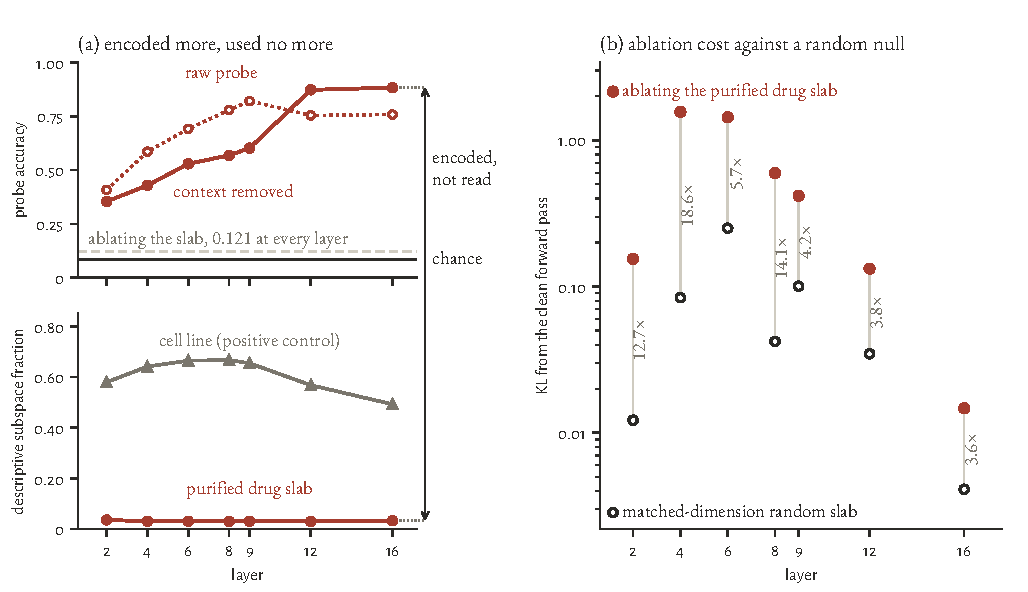
\includegraphics{fig-mechanism}
  \caption[Decodable with depth, at limited functional weight]{\captiontitle{Drug-label
  information becomes more decodable with depth while interventions on the
  purified slab have limited effect.} Layer is a true numeric axis in both panels.
  \emph{(a) Top:} probe accuracy over twelve drug classes, chance $1/12$. The raw
  series and the context-removed series \emph{cross} between layers $9$ and $12$,
  which no other figure shows; the flat grey line is the same probe after the drug
  slab is projected out. \emph{Bottom:} subspace fraction of the purified slab
  against the cell-line control, on its own scale --- an activation-space summary,
  not a decomposition of biological variance. \emph{(b)} Mean KL in nats when the
  slab is ablated, against a matched-dimension random slab, $n = 60$ per entry.
  Log axis, so the vertical gap between a pair is their ratio. No intervals are
  drawn in either panel. These accuracies are twelve-class and must not be read
  against the twenty-four-class sweep of \cref{sec:res-mechanism}.}
  \label{fig:mechanism}
  \end{fullwidth}
  \end{figure}
  
  

\paragraph{Step two, purification} The subspace step one returns is partly a
batch subspace. Drug, plate and dose are confounded by the atlas's design, so
directions fitted to separate the twelve drugs will also separate whatever
those drugs were plated and dosed alongside. That this has happened is not
assumed but measured: projecting the activations onto the slab and fitting the
same cross-validated logistic probe to the projected coordinates
$X V_{\textrm{drug}} \in \mathbb{R}^{n \times k}$ --- ten numbers per prompt,
nothing else --- recovers each prompt's \emph{dose} at $0.90$ to $0.95$ at
every layer. A subspace built only to carry drug identity should not be able to
do that, and a null obtained by removing it would not distinguish deleting the
drug from deleting the batch it arrived in.

The remedy is to subtract that shared structure. A context subspace
$V_{\textrm{conf}}$ is built exactly as $V_{\textrm{drug}}$ was, but from three
labels at once rather than one. Cell line, plate and dose are each categorical
labels carried by every prompt, and each cuts the same $\num{480}$ rows a
different way: by which cell line the cell came from, by which physical plate
it was assayed on, by which concentration it received. Write
$\mathcal{L} = \{\textrm{cell line}, \textrm{plate}, \textrm{dose}\}$, and for
each $L \in \mathcal{L}$ let $\mathcal{C}_L$ be the distinct values that label
takes in this sample --- the individual cell lines that appear, the individual
plates, the individual dose levels --- so that a single $c \in \mathcal{C}_L$
picks out one cell line, or one plate, or one dose. For each such $c$ write
$n^{L}_{c} = |\{ i : L(x_i) = c \}|$ for how many of the $\num{480}$ prompts
carry it, and
\begin{equation}
  \mu^{L}_{c} \;=\; \frac{1}{n^{L}_{c}} \sum_{i \,:\, L(x_i) = c} x_i
\end{equation}
for their mean activation, computed over the same rows and centred on the same
global mean $\bar{x}$ as in step one. Collect one row per qualifying value,
across all three labels:
\begin{equation}
  M_{\textrm{conf}} \;\in\; \mathbb{R}^{m \times d},
  \qquad
  \textrm{rows} \;=\; \big\{ (\mu^{L}_{c} - \bar{x})^{\top} \;:\;
    L \in \mathcal{L},\; c \in \mathcal{C}_L,\; n^{L}_{c} \geq 5 \big\},
\end{equation}
\begin{equation}
  m \;=\; \sum_{L \in \mathcal{L}}
          \big| \{\, c \in \mathcal{C}_L : n^{L}_{c} \geq 5 \,\} \big| ,
\end{equation}
so $m$ counts every cell line, plate and dose level with at least five prompts
behind it, summed across the three labels --- of order tens of rows against the
drug slab's twelve, and each of length $d$. Its singular value decomposition is
truncated by the same relative spectral rule as step one,
\begin{equation}
  V_{\textrm{conf}} \;=\; \big[\, w_1 \;\cdots\; w_{k'} \,\big]
  \;\in\; \mathbb{R}^{d \times k'},
  \qquad
  k' \;=\; \min\!\big( 3k_{\max},\;
           \#\{ j : \sigma_j > 0.05\,\sigma_1 \} \big),
\end{equation}
with $k_{\max} = 10$ the drug slab's dimension budget. Stacking the three label
sets together rather than fitting them separately matters: cell line, plate and
dose are themselves correlated in this atlas, and three independently fitted
subspaces would subtract their shared directions three times over. One matrix
spans their union once. The budget is three times the drug slab's for the
opposite reason --- context genuinely needs more directions than drug does,
since it is carrying three partitions rather than one, and a budget that bound
here would leave real batch structure unsubtracted and inside
$V_{\textrm{pure}}$.
The drug slab is then projected off it and re-orthonormalised. First subtract
the component lying inside the context subspace,
\begin{equation}
  \widetilde{V} \;=\; V_{\textrm{drug}} \;-\;
    V_{\textrm{conf}} V_{\textrm{conf}}^{\top} V_{\textrm{drug}}
  \;\in\; \mathbb{R}^{d \times k},
\end{equation}
whose columns are no longer orthonormal, and in general no longer of unit
length, since each has lost whatever part of itself the context could account
for. Recover an orthonormal basis by QR decomposition,
\begin{equation}
  \widetilde{V} \;=\; QR ,
  \qquad
  Q \in \mathbb{R}^{d \times k} \ \textrm{orthonormal},
  \qquad
  R \in \mathbb{R}^{k \times k} \ \textrm{upper triangular},
\end{equation}
and keep only the columns whose surviving component was substantial,
\begin{equation}
  V_{\textrm{pure}} \;=\; \big[\, q_j \;:\; |R_{jj}| > 0.2 \,\big].
\end{equation}
The diagonal of $R$ is what makes that threshold meaningful. Because
$V_{\textrm{drug}}$'s columns are unit norm to begin with, $|R_{jj}|$ is
literally the fraction of column $j$ left standing after the projection: a
value near one means the direction was almost entirely orthogonal to context
already, and a value near zero means it was almost entirely context. Keeping
only those above $0.2$ is what stops a direction that barely survived from
being retained and then renormalised back to unit length by $Q$, which would
amplify context and estimation noise rather than remove it. Two screens guard the same step from the other side. A
candidate context label is dropped before it can enter $V_{\textrm{conf}}$ if
it is more than $90\%$ pure as a proxy for the drug, since orthogonalising
against a relabelled copy of the drug would delete the drug axis by
construction and manufacture any null that followed; and classes with fewer
than five members are skipped, so that a near-continuous field like dose cannot
degenerate the context subspace into a generic top-variance basis.

What remains, $V_{\textrm{pure}}$, is the part of the drug slab that no context
label can account for, and it is what every causal claim below is made on ---
never the raw slab. \Cref{fig:purify} draws the construction.

% ===========================================================================
\begin{table}[htbp]
% MARGINALIA: full-width pattern (caption above at the text width, notes below
% in the sans). The table itself is natural width; the caption is too long for
% the margin. One rule; the spanner row replaces the \cmidrule. The long
% sub-head is stacked so its column shrinks to the numbers.
    \caption{\captiontitle{Drug-label information becomes more decodable with depth while
    the same slab carries little functional weight.} All seven layers pass the
    removal gate; chance is $0.083$. Columns under \emph{Decode} and
    \emph{Ablation} are labelled by which subspace was projected out of the
    residual stream before measuring: the two decode columns are the same
    twelve-class probe on the same activations, once with nothing removed and once
    with the context subspace $V_{\textrm{conf}}$ --- cell line, plate and dose ---
    projected out, and neither is restricted to the drug slab. The random null
    matches $V_{\textrm{pure}}$'s rank, not the variance it removes --- the slab's
    subspace fraction is roughly six times the null's --- so that ratio mixes drug
    content with the difference.}
    \label{tab:workspace}
  \begin{fullwidth}
  \begin{threeparttable}
    \begin{tabular}{@{}r rr rrr rr@{}}
      & \multicolumn{2}{l}{\thead{Decode accuracy}}
      & \multicolumn{3}{l}{\thead{Ablation cost (KL, nats)}}
      & \multicolumn{2}{l}{\thead{$V_{\textrm{pure}}$ against}} \\
    \addlinespace[2pt]
    \thead{Layer} & \thead{Original}
      & \shortstack[r]{\thead{$V_{\textrm{conf}}$}\\\thead{projected out}}
      & \thead{$V_{\textrm{pure}}$} & \thead{random} & \thead{$V_{\textrm{cell}}$}
      & \thead{random} & \thead{$V_{\textrm{cell}}$} \\
    \midrule
    2  & 0.408 & 0.354 & 0.155 & 0.012 & 1.115 & $12.7\times$ & $14\%$ \\
    4  & 0.585 & 0.429 & 1.563 & 0.084 & 4.180 & $18.6\times$ & $37\%$ \\
    6  & 0.692 & 0.529 & 1.435 & 0.251 & 4.307 & $5.7\times$  & $33\%$ \\
    8  & 0.779 & 0.569 & 0.596 & 0.042 & 5.419 & $14.1\times$ & $11\%$ \\
    9  & 0.821 & 0.602 & 0.418 & 0.100 & 4.689 & $4.2\times$ & $9\%$ \\
    12 & 0.754 & 0.873 & 0.133 & 0.035 & 0.135 & $3.8\times$  & $98\%$ \\
    16 & 0.758 & \key{0.883} & 0.015 & 0.004 & 0.059 & $3.6\times$ & $25\%$ \\
    \end{tabular}
    % no [flushleft]: that option redefines \TPTnoteSettings and would override
    % the preamble's sans-8pt quietink note setting (already flush left).
    \begin{tablenotes}
    \item The two decode columns answer different questions and are not two
    estimates of one quantity: the first includes whatever cell line, plate and
    dose contribute, the second is the same probe once those directions are gone.
    \item Every ablation cost collapses at layers $12$ and $16$, the positive
    control most of all --- $V_{\textrm{cell}}$ falls from $4.689$ nats at layer
    $9$ to $0.135$ at layer $12$. Layer $12$'s $98\%$ is therefore a small
    numerator over a smaller denominator, not a depth at which the drug slab
    matters more.
    \end{tablenotes}
  \end{threeparttable}
  \end{fullwidth}
  \end{table}
\paragraph{Step three, the removal gate} A null from an ablation is only
evidence if the thing removed was really there. Delete a subspace the model
never encoded the drug into, and generation will of course not move --- and
that outcome is indistinguishable, from the output alone, from a subspace that
carried the drug and simply went unread. The gate settles which of the two is
happening, before any null is reported.

The test reuses the probe of \cref{sec:methods-probe} and runs it twice at each
depth. First on the activations as they are, giving accuracy $a$; then on the
activations with the drug subspace projected out, $X \leftarrow X - (X
V_{\textrm{drug}})V_{\textrm{drug}}^{\top}$, giving $a_{\textrm{abl}}$. What the
gate scores is not the drop itself but the \emph{fraction of above-chance
signal} it accounts for, measured against the twelve-class floor $\pi = 1/12$
rather than against zero,
\begin{equation}
  f \;=\; \frac{a - a_{\textrm{abl}}}{a - \pi} ,
\end{equation}
and $f$ must exceed $0.8$ for the depth to pass. Measuring against $\pi$ is what
makes $f$ interpretable: a probe cannot fall below chance in expectation, so
$a - \pi$ is the whole of what the subspace could possibly have been carrying,
and $f$ asks how much of that the projection actually took.

The gate passes at all seven depths. It is the raw accuracy $a$ that varies
across depth, from $0.41$ at layer $2$ to $0.82$ at layer $9$; the ablated
accuracy $a_{\textrm{abl}}$ does not vary at all, sitting at $0.121$ wherever
the projection is applied, a floor just above the $1/12$ the label set puts
chance at. Projecting the subspace out therefore does not merely degrade the
probe, it returns it to the same near-chance state at every depth, whatever it
was reading before.

Because $a_{\textrm{abl}}$ is fixed, the whole spread in the removed fraction
comes from $a$. Where the raw probe is strongest the subspace accounts for
almost everything it was reading --- $0.949$ at layer $9$ --- and where it is
weakest the fraction is smallest, $0.885$ at layer $2$, giving the $88$ to
$95\%$ band. The ordering matters more than the range: the gate is hardest to
clear exactly where the probe has least signal to begin with, since a fixed
floor leaves proportionally more of a small gap standing, and it clears there
too. \Cref{fig:purify}, panel (c), draws all seven; the shaded region below the
rule is the set of outcomes that would have left every null in this section
untestable, and it is empty. The nulls reported below are therefore properties
of the model rather than of a hook that missed.

% ===========================================================================
\begin{figure}[htbp]
\begin{fullwidth}
\centering
% ===========================================================================
% figs/purify.tex -- fig:purify, how the drug slab is BUILT, and the gate it
% has to pass before anything may be ablated with it.
%
% FIGURE BODY ONLY. No preamble, no document environment, no float, no caption.
% \input it from inside a figure/fullwidth float in
% Sections/04b-representation.tex; the ready-to-paste float sits commented at
% the foot of this file and is also staged in figs/_PENDING_FLOATS.tex.
% Compiles against thesis_v2/preamble.tex and nothing else: no \includegraphics,
% no external data, no TikZ library beyond the ones preamble.tex already loads
% (this file uses arrows.meta and calc only).
%
% WHAT THE FIGURE IS
% ------------------
% Steps one to three of sec:res-used, drawn as steps. Step one localises the
% drug: twelve centred class means, ten kept directions. Step two purifies it:
% the raw slab is orthogonalised off the context it is confounded with. Step
% three is the falsifiability check: projecting the slab out must destroy most
% of the decodable drug signal, or every null downstream is a measurement of
% nothing. fig:hook (a separate float, six paragraphs later) draws step four;
% the two are deliberately NOT merged -- each is about 100mm tall, the corpus
% ceiling is slab.tex at 117mm, and the house caption shape carries one bolded
% finding, not two.
%
% EVERY NUMBER DRAWN, AND WHERE IT COMES FROM
% -------------------------------------------
% Source for every measured quantity: RESULTS_cluster/workspace_probe.json.
% Config there: tier tier2_unseen_drugs, n_drugs 12, n_per_drug 40, n_dims 10,
% layers 2,4,6,8,9,12,16, chance 0.08333333333333333, seed 42.
% Sibling ledger with the full machine-precision values: figs/purify.json.
%
% (a) THE SEVEN PLOTTED DOTS -- the only marks in this figure with a scale.
%     layers.<L>.frac_signal_removed, layers 2,4,6,8,9,12,16:
%       0.8846153846153847  0.9253112033195021  0.9383561643835617
%       0.9461077844311377  0.9491525423728814  0.9440993788819876
%       0.9444444444444445
%     layers.<L>.gate_pass is true at all seven; the dots' position above the
%     0.8 rule is that fact, so no second mark asserts it.
%
% (b) THE GATE, 0.8. PROSE ONLY. Sections/04b-representation.tex:185 "the
%     fraction of above-chance signal removed must exceed $0.8$". There is no
%     config field for it in workspace_probe.json, so the ledger cites the .tex
%     line and not a key path. Drawn dashed accent, the house register for a
%     pre-set threshold a value is tested against (gate.tex:170-174).
%     SUPERSEDED IN v10 BELOW: it is now black, solid, 0.9pt.
%
% (c) THE THREE PRINTED ACCURACIES in the right-hand block of band two.
%       before  0.41--0.82   layers.2.drug_decode  = 0.4083333333333334
%                            layers.9.drug_decode  = 0.8208333333333334
%       after   0.121        layers.<L>.drug_decode_ablated
%                            = 0.12083333333333332, byte-identical at all seven
%       chance  0.083        top-level chance = 0.08333333333333333
%     Thesis 04b:186-188 "Accuracy falls from $0.41$--$0.82$ to a constant
%     $0.121$ floor, removing $88$--$95\%$ of the above-chance signal".
%     SUPERSEDED IN v10 BELOW as to PLACEMENT only: the three values are no
%     longer a right-hand gutter block, they are the figure's foot note. No
%     value changed.
%
% (d) THE IDENTITY, verified numerically before drawing, in python, over all
%     seven layers, exact float equality (not a tolerance):
%       (drug_decode - drug_decode_ablated) / (drug_decode - chance)
%         == frac_signal_removed
%     Layer 2: (0.4083333333333334 - 0.12083333333333332)
%              / (0.4083333333333334 - 0.08333333333333333)
%              = 0.8846153846153847, bit for bit.
%     WHICH SLAB THE GATE IS MEASURED ON. This identity fixes it, and the
%     answer is NOT V_pure. workspace_probe.json stores exactly one ablated
%     series, drug_decode_ablated, and the identity reproduces from the RAW
%     decode. The section-4.5 arm files prove the pipeline can distinguish the
%     two cases -- they store drug_decode_ablated AND drug_decode_pure_ablated,
%     frac_signal_removed AND frac_signal_removed_pure -- and this file stores
%     only the first of each pair. So the figure, the caption and the ledger all
%     say "the slab that is projected out" and nowhere claim the gate was run on
%     V_pure. Stage two's arrow lands on V_pure because that is where the CAUSAL
%     claims are made (04b:179-180); band two is a separate measurement and the
%     divider is what keeps the two from being read as one.
%     SUPERSEDED IN v10 BELOW as to the LAST CLAUSE ONLY: the divider is gone
%     and the panel letters do that work now. The caveat itself survives, in the
%     foot note.
%
% (e) THE FOUR PRINTED NUMBERS IN STAGE TWO, the only measured quantities above
%     the divider.
%       0.90--0.95   layers.<L>.confound_crossdecode.dose, seven layers:
%                    0.9020833333333333 0.9229166666666666 0.9416666666666667
%                    0.9395833333333332 0.95 0.8979166666666666
%                    0.8979166666666668. Thesis 04b:176-178.
%                    PRINTED AS TEXT AND NOT DRAWN, and there is deliberately NO
%                    0.90 reference rule anywhere in this figure: the stored
%                    minimum is 0.8979166666666666 at layers 12 and 16 and
%                    reaches the thesis's "0.90" only by rounding to two places.
%                    A rule at 0.90 would put two of seven points below it and
%                    would read as a failure the thesis does not report.
%       raw 0.620    layers.9.variance_share.drug      = 0.6201207831136324
%       purified     layers.9.variance_share.drug_pure = 0.030620247335072275
%         0.031
%     The RAW share is quoted in no sentence of the thesis; figs/fig-mechanism.json
%     already records it as drug_raw_not_drawn. Printing it here is a new reading
%     of a stored field, flagged as such in purify.json, on the precedent of
%     figs/slab.json's handling of variance_share.context. Layer 9 is named in
%     the figure text so the pair cannot be read as a seven-layer summary; it is
%     the layer at which the raw probe peaks (04b:170-171), which is why the
%     section uses it as its own reference depth.
%
% (f) THE COUNTS in stage one: 480 prompts, twelve drugs, forty cells each,
%     seven layers, ten kept directions, span at most eleven.
%     config.n_drugs 12, config.n_per_drug 40, config.n_dims 10,
%     layers.<L>.pure_drug_dims 10, config.layers "2,4,6,8,9,12,16".
%     480 = 12 x 40 and the rank-11 bound (twelve centred means span at most
%     eleven directions) are ARITHMETIC, not stored fields; the ledger says so.
%     Thesis 04b:164-171.
%
% AGREEMENT WITH THE TEXT (checked line by line, not assumed):
%   04b:164-165  "\num{480} tier-2 prompts (twelve drugs, forty real cells
%                each) at seven layers"            -> stage one, line 4.     OK
%   04b:168-170  "Twelve centred class means span at most eleven directions,
%                so the slab keeps essentially the whole span, noisiest
%                included, which for a removal claim is conservative"
%                -> stage one, lines 1-3, verbatim.                          OK
%   04b:175-178  "The raw drug slab is partly a batch slab. Drugs are
%                confounded with plate and dose by the atlas's design, and
%                probing dose from inside the drug subspace recovers it at
%                $0.90$--$0.95$ at every layer"    -> stage two, lines 1-3.  OK
%   04b:179-180  "Every causal claim below is made on $V_{\textrm{pure}}$,
%                never on the raw slab."           -> the V_pure callout.    OK
%   04b:185-186  "the fraction of above-chance signal removed must exceed
%                $0.8$; below that the null is unfalsifiable, a measurement
%                of nothing"                       -> the dashed rule, and
%                                                     G4's two italic lines,
%                                                     which are the section's
%                                                     own words.             OK
%   04b:186-188  "Accuracy falls from $0.41$--$0.82$ to a constant $0.121$
%                floor, removing $88$--$95\%$"     -> right-hand block and
%                                                     the set label.         OK
%   04b:212-213  tab:workspace caption "All seven layers pass the removal gate
%                (88--95\% ...); chance is $0.083$"                          OK
%
% AVAILABLE, DELIBERATELY NOT DRAWN, recorded here and in purify.json so a
% reviewer who asks for direct evidence of the batch overlap is answered
% without a redraw:
%   * layers.<L>.overlaps.context   0.5215396547181934 -- 0.6323768458353303
%   * layers.<L>.overlaps.cell_line 0.3043896441494730 -- 0.3534060289850234
%     These are the per-layer measure of "the raw drug slab is partly a batch
%     slab" and are quoted nowhere in the thesis. Drawing them would put a
%     second measured scale into a panel whose whole discipline line says the
%     geometry has no scale, and would be a new claim rather than a redraw.
%   * layers.<L>.confound_crossdecode.plate, 0.4541666666666667 --
%     0.5770833333333333, a materially weaker and entirely undiscussed
%     confound. Not printed, because the section names dose and not plate.
%   * layers.<L>.swap.{drug_b_kl, random_inject_kl} in this same JSON is the
%     RETIRED steering design (07-Appendix.tex, sec:app-identity). Nothing from
%     it is on this figure. figs/mechanism.py's header records that the v1
%     figure plotted exactly that pair while its caption described the ablation.
%
% DESIGN DECISIONS, each with its reason
% --------------------------------------
%  1. TWO BANDS AND A DIVIDER THAT IS A STATEMENT. Above the rule at y=4.72
%     nothing has a scale; below it everything does. No mark crosses the rule,
%     no leader connects a schematic object to a plotted one, and the italic
%     sentence under the rule sets band two up as the answer to the objection
%     stage two raises -- if purification strips the raw slab from 0.620 to
%     0.031 of the stream's variance, does anything survive in it? The
%     alternative, one continuous diagram from cloud to axis, was rejected: it
%     would invite the reader to measure the ellipse.
%     SUPERSEDED IN v10 BELOW. The divider and its sentence are deleted; the
%     schematic/measured distinction is now carried by the MARK (open rulegrey
%     ring against filled accent disc), which is where it belongs.
%  2. THE FAIL REGION IS DRAWN, THE PASS REGION IS NOT. The one non-obvious
%     mark in band two is the rulegrey!18 rectangle from 0 to 0.8. It is the
%     region of outcomes that would have made every null in this section a
%     measurement of nothing, and it is empty. A figure that drew only the seven
%     dots and the rule would be a bar of good news; drawing the region the
%     dots had to avoid is what makes it a falsifiability picture. Its emptiness
%     is also where the two italic lines fit, which is not a coincidence and is
%     the reason they are placed there rather than in the caption.
%     PARTLY SUPERSEDED IN v10: the region survives, at rulegrey!12, and the two
%     italic lines inside it do not. The emptiness is the message and text in it
%     was competing with the marks.
%  3. NO CONNECTING LINE THROUGH THE SEVEN DOTS. The series is flat to 0.1355cm
%     on this scale (0.8846 to 0.9492 at 2.10cm per unit of fraction). A line
%     would assert a trend across a 6-point spread the axis cannot resolve; the
%     seven marks are named as one ordered set by "all seven layers: 88--95%"
%     instead, which is comparators.tex's rule for marks too close to leader
%     individually.
%  4. NO INTERVALS ANYWHERE. frac_signal_removed is a single ratio of two
%     accuracies on 480 prompts and carries no stored dispersion of any kind;
%     the KL series in the same file carry normal-approximation SEs, which are
%     not this document's interval convention (figs/fig-mechanism.json records
%     intervals_drawn false with that reason). A bare solid dot with no bar is
%     how this document says a quantity has no interval (comparators.tex:149-151
%     changed a hollow ring to a solid dot for exactly this).
%  5. THE ORTHOGONALISATION IS DRAWN AS AN OPERATION, NOT AS A RESULT, AND THE
%     OPERATION IS A PROJECTION AND NOT A ROTATION. This is the one mark
%     figs/slab.tex does not have. There the drug wedge and the
%     context wedge are simply shown already orthogonal, which states the
%     outcome and hides the step; here the raw band sits at 38 degrees, visibly
%     crossing the context band, and the raw slab's tip is carried onto V_pure.
%     REPAIRED, PASS 9. It used to be carried by an accent ARC from 38 to 76
%     degrees, i.e. the raw band swung upright. A reviewer read that panel as
%     "the slab is turned until it is perpendicular to context" and had to go to
%     the prose to learn that a component is REMOVED, and they were right to:
%     two bands of equal width (0.32cm) and near-equal length (1.90 against
%     2.00) differing only in angle say "same slab, rotated, nothing lost",
%     against measured numbers 1.8cm to the right that say raw 0.620, purified
%     0.031, a twentyfold shrink. A curved arrow is the universal sign for
%     rotation. What replaces it is the subtraction itself: a dashed rulegrey
%     perpendicular from the raw band's tip down to the context band, the
%     component it lands on drawn as its own named mark, and a STRAIGHT accent
%     arrow at the tip's own height carrying the tip left by exactly that
%     component, landing on V_pure. Two further faults the arc had, both from
%     the render: its head stopped 1.5mm short of the V_pure bar and pointed at
%     white space, and the grey leader from the word "orthogonalise" stopped 4mm
%     short of the arc's tail -- the corpus puts the 0.06cm gap at the LABEL
%     end, never at the mark end, so that stub read as a stray hairline. The
%     label now sits 0.15cm from the arrow's tail and carries no leader, and the
%     arrow is 0.6pt: a schematic operation, not a measurement, where 1.0pt is
%     the corpus's "this IS the claim" register. V_pure was also narrowed from
%     0.32 to 0.18cm, so the purified band is visibly thinner than the raw one.
%     slab.tex is left alone and is not
%     superseded: three of its four panels are the failed identity designs of
%     sec:app-identity, which are the appendix's argument, and its magnified
%     interior is sec:res-mechanism's swap geometry. What it draws that belongs
%     to sec:res-used is one thing, the variance-share disc, and this figure
%     does not redraw it. The two figures share vocabulary (accent-on-white
%     bands, rulegrey leaders, one discipline line saying what is to scale) and
%     no coordinate.
%     The whole of this decision survives v10 except the arrow's WEIGHT, which
%     goes 0.6 -> 0.5pt to bring the file inside a four-weight budget; the
%     perpendicular goes dashed-rulegrey -> densely-dotted-quietink, which is
%     this document's reserved stroke for a projection line.
%  6. THE CONFOUND IS A NAMED MARK, NOT THE PRODUCT OF TWO TINTS.
%     REPAIRED, PASS 9, and this is the repair both reviewers called blocking.
%     It used to be the lozenge where the raw band's tint multiplied over the
%     context band's, with the whole claim carried by the caption ("that
%     darkened region is the confound step two exists to remove"). Three faults:
%     (a) it was the only element in the panel with no direct label, while every
%     other mark had one; (b) V_pure ran vertically through its centre and split
%     it in two -- sampled on the render, a row across it read grey (174,174,174),
%     then (119,143,164) for the tint product, then a hard cut to opaque accent
%     (11,82,147) for 24px, then (119,143,164) again -- so it was not a nameable
%     region at all; (c) it made a CROSSING mean "confounded" on a panel where
%     another crossing, V_pure through the same band, has to mean "orthogonal".
%     One glyph cannot carry both. It is now the orthogonal projection of the
%     raw direction onto context: a segment along the context band from the
%     shared origin to the foot of the perpendicular dropped from the raw band's
%     tip, drawn in the raw slab's own tint at a higher opacity with a 0.35pt
%     accent!70 outline, and directly labelled "the confound". It begins at
%     V_pure's right edge, so nothing bisects it, and it is exactly the length
%     of the removal arrow above it, which is the rhyme that makes the arrow
%     legible. With the tint-multiply claim gone, a crossing means nothing
%     anywhere in the panel and the right-angle mark is the only assertion of
%     orthogonality, which is what decision 8 already wanted.
%     The context band is now panelbg with a rulegrey outline and not ink!35:
%     see decision 11.
%  7. NO 0.90 REFERENCE RULE. See (e) above: the stored dose minimum is
%     0.8979166666666666 and rounds to the thesis's 0.90. Printing the range as
%     text states exactly what the section states; a rule would show two of
%     seven points below it and would manufacture a failure.
%  8. RIGHT ANGLE AS A MARK, NOT AS A WORD. The small square in the
%     upper-left quadrant at the shared origin is the only assertion that
%     V_pure and the context subspace share no direction. The word
%     "orthogonalise" labels the operation; the square labels its result.
%     PASS 9: ink 0.35pt, up from rulegrey 0.3pt. The caption calls it "the one
%     geometric fact true by construction" and it was the faintest mark in the
%     panel.
%     AMENDED IN v10: the square moves to the LOWER-left quadrant, doubles to
%     0.40cm arms, and acquires the direct label it never had.
%     SUPERSEDED IN v11: THIS LINE IS FALSE ABOUT ITS OWN DRAWING AND ALWAYS
%     WAS. v10 drew the square in the UPPER-left quadrant of the crossing --
%     (10.01,8.65)-(10.01,9.05)-(10.41,9.05) -- and no build has ever put it
%     lower-left. The direct label and the enlargement are true. v11 keeps the
%     upper-left quadrant, which is the only one of the four that is free (the
%     raw band at 38 degrees crosses lower-left and upper-right, and "the
%     confound" and its leader own lower-right), and takes the arms 0.40 ->
%     0.28cm to clear the removal arrow -- see v11 item 2.
%  9. THE GLOBAL MEAN IS A CROSS, NOT A DOT. The twelve class means are dots;
%     the thing they are centred on must not be a thirteenth dot. It is also
%     leadered out of the cloud rather than labelled in place, because at
%     8pt the label box collided with two of the twelve dots.
% 10. V_drug IS DRAWN WITH STAGE TWO'S OWN GLYPH, AND ALL TWELVE DISPLACEMENTS
%     ARE DRAWN. REPAIRED, PASS 9, two findings at once.
%     (a) V_drug used to be a dashed, accent!10 FILLED ELLIPSE enclosing the
%     twelve dots, while stage two drew the same name as an unbounded band. A
%     bounded blob around the class means says "the region where the drugs
%     live"; a subspace is not a region and has no edge. Read cold, the ellipse
%     was taken for the data cloud and stage two's band for a new object, so
%     stage one's output was never connected to stage two's input -- the one
%     join the figure exists to make, and the join the brief says readers lose.
%     V_drug is now an accent band at the SAME fill opacity stage two uses,
%     through the global mean, running past the data on both sides. The ellipse
%     is deleted rather than kept unlabelled: with the band tall enough to
%     contain all twelve dots (half-height 0.52 against a maximum |dy| of 0.44)
%     it had nothing left to say, and a class mean drawn OUTSIDE V_drug would
%     have been false, since the twelve centred means span it by construction.
%     (b) ONE displacement was drawn and eleven were not, so "twelve are
%     stacked" -- the sentence directly under the dots -- was invisible, and the
%     dots were unlabelled while the prose two lines below names a different
%     population ("480 prompts: twelve drugs, forty real cells each"), so the
%     scatter read as prompts and the cross as their grand mean. All twelve
%     stems are now drawn at 0.3pt quietink, with the one accent arrow on top
%     and still the only labelled one, and the dots carry the tag "the twelve
%     per-drug means". The stems make the count a picture and they are what the
%     "at most eleven directions" line is about.
%     The twelve offsets are written out in a \foreach list so no build can
%     randomise them and no reader can be told a different story by a different
%     compile. Opacity: the band is 0.20, not the 0.34 of stage two's first
%     draft, and stage two's raw band was brought to 0.20 with it. At 0.34 over
%     5.10 x 1.04cm the band became the single heaviest area on the page, which
%     is the thing this figure was already being marked down for; at 0.20 over
%     4.10 x 1.04 it lays down about the ink of stage two's 1.90 x 0.32 band and
%     the two are drawn at the SAME opacity, so the glyph rhymes exactly.
%     AMENDED IN v10: the twelve class means become OPEN RINGS and the one
%     accent displacement arrow loses its head -- see v10 items 3 and 6.
% 11. ONE GREY FAMILY, AND THE CONTEXT SUBSPACE IS THE COLOUR slab.tex GIVES IT.
%     PASS 9. Three greys were in play, derived two different ways: rules at
%     rulegrey, the context band at ink!35, the gate region at rulegrey!18.
%     ink!35 is not derived from rulegrey and is LIGHTER than a hairline rule,
%     so the band read as a heavy solid slab while the rules read as thin, and
%     it was the darkest region on either page. slab.tex draws this same named
%     subspace in panelbg (its \slabdisc, slab.tex:83-90), so the figure also
%     disagreed with the published figure about what colour the object is. The
%     band is now panelbg with a 0.35pt rulegrey outline; ink!35 no longer
%     appears in the document, and purify's context band and slab.tex's context
%     wedge are the same object drawn twice.
% 12. THE GATE PANEL KEEPS ITS FULL 0-TO-1 AXIS. A reviewer asked for the range
%     to be cut to 0.75-1.00 so the seven fractions (0.8846 to 0.9492, 0.1355cm
%     apart on this scale) would resolve, against a fail region 12.4x their
%     height. OVERRULED, and the reason is the same one that bans bars on a log
%     axis: the fail region's height is not a drawing choice, it is the share of
%     the outcome space that would have made every null below unfalsifiable, and
%     0 is the natural floor of a fraction, not an arbitrary cut. Cutting the
%     axis at 0.75 would shrink the one region whose SIZE is the argument, to
%     resolve an ordering the thesis makes no claim about -- tab:workspace is
%     the authority for the per-layer values and the section quotes only the
%     range. What was applied instead: the direct label "all seven layers:
%     88--95%" names the set (decision 3), and the 0.8 numeral was dropped from
%     the tick set because the accent label already owns that coordinate.
%     STILL IN FORCE IN v10, and it is the first thing v10 was told to protect.
%
% WHAT SIX RENDER-AND-READ PASSES CHANGED, with the measurement that forced it
% ---------------------------------------------------------------------------
%  i.   PASS 1, Overfull 88.29pt. The discipline line under stage two ran 146
%       characters at \footnotesize and measured 20.4cm against a 17.30cm
%       measure. Cut to 103 characters; the sentence now states only what it
%       has to, that the geometry has no scale and four numbers do.
%  ii.  PASS 1. "every causal claim is made here", set anchor=south at y=9.22,
%       put its box top at 9.63 against the stage-two subtitle's ink bottom of
%       9.37 and the two overprinted. There is no room above V_pure for a
%       second line, so the sentence became the fourth line of stage two's
%       prose block, in the section's own words ("never on the raw slab").
%  iii. PASS 1. "the global mean" and "$\mu_d-\bar\mu$, one drug's" collided
%       character to character: both wanted the space up and right of the
%       cloud, which is where the displacement arrow points. The global mean
%       was moved BELOW the cloud on a leader. Drawn straight down that leader
%       read as a dropped axis, so PASS 4 gave it a 0.25cm dogleg; the dogleg
%       clears the two nearest class means by 0.23cm and 0.25cm.
%  iv.  PASS 2, Overfull 6.20pt, unchanged from PASS 1 by three edits, which is
%       what identified it: the culprit was not the widest LINE but the
%       fraction axis's own tick label. "1.0" is anchor=east on a spine at
%       x=0.30, and its box ran 0.28cm LEFT of x=0. The bare \path pins a
%       minimum box, not a maximum, so nothing clipped it. The whole plot was
%       shifted right (spine 0.30 -> 0.75, layer 2 from 0.60 -> 1.05) rather
%       than the label being clipped or shrunk. boxes=0 from PASS 4 on.
%  v.   PASS 2. Band two carried two annotation columns 0.30cm apart at the
%       same baseline, so "88--95%" and "accuracy before" read as one line. The
%       plot was widened from 8.60 to 11.00cm of layer axis and the two columns
%       became one, which also removed 3.4 x 1.9cm of dead white under them.
%  vi.  PASS 4, at 520dpi. The leader to "orthogonalise" left the arc 0.20cm
%       from its own arrowhead and read as a grey continuation of the accent
%       arrow. It now leaves at 50 degrees, 0.42cm clear of the head, and stays
%       above the raw band's upper edge for its whole length. The right-angle
%       mark went from 0.16 to 0.20cm, and the global-mean cross from 0.30 to
%       0.45pt with 2mm arms, because at 0.3pt it was fainter than the leaders.
%  vii. PASS 5. Stage one left 4.2 x 1.9cm of white to the right of the cloud
%       while stage two's matching region was full. The ellipse went from
%       1.75 to 2.05 x-radius and the cloud from 1.45 to 1.72, which both fills
%       the panel and raises the aspect from 2.34:1 to 2.77:1. The ellipse's
%       y-radius was NOT raised with it: at 0.98 the ellipse reached y=6.92 and
%       left the global-mean label 0.06cm from the prose block below.
%  viii.PASS 5. The panel-three subtitle said "projecting the slab out", which
%       after stage two's "every causal claim is made on V_pure" invited the
%       reading that the gate was run on V_pure. It now says "projecting the
%       drug subspace out", the section's own noun at 04b:184-185, and the
%       string V_pure does not appear in panel three at all.
%
% LAYOUT NOTES, all forced by a build
% -----------------------------------
%   * fullwidth = textwidth 142mm + marginparwidth 28mm + marginparsep 4mm
%     = 174mm. (The "171mm" beside \newenvironment{fullwidth} in preamble.tex
%     is stale arithmetic.) The bounding box is pinned with a bare \path at
%     (0,-0.12) rectangle (17.30,10.20) = 173.0 x 103.2mm, inside the 17.35cm
%     hard edge circularity.tex records and under the corpus height ceiling,
%     slab.tex at 117mm. The harness reports pages=1, boxes=0. It grew 1.7mm in
%     pass 9: band two moved down 0.20cm to open a line under stage three's
%     subtitle for the "which slab" caveat, and the "four ... see fig:hook"
%     pointer sits on the bottom line. The float got much SHORTER overall in the
%     same pass, because the caption went from 484 words to about 280.
%   * x=1cm, y=1cm. Nothing is scaled, nothing is \resizebox'd; 1cm here is
%     1cm on the page.
%   * pgfmath: \lx and \fy expand to BRACED groups, so \lx{2}+0.05 is not a
%     coordinate. Every stand-off is either inside the braces or an xshift on
%     the node (gate.tex records the same trap).
%   * the tick rows use the \v/\t value/label pair form, so the fraction axis
%     prints 0.5 and 1.0 rather than \foreach's raw 0.5 and 1 tokens. The layer
%     row does not need it: its values are integers and print as themselves.
%   * no node uses align= or text width=: such a node builds a minipage whose
%     first-line height follows the AMBIENT \baselineskip, so its ink moves
%     with whatever prose precedes the float (frames.tex measured 3.7pt of
%     drift). Every multi-line block here is a stack of single
%     anchor=base west lines on explicit baselines: 0.28cm apart in band one's
%     two prose blocks, 0.33cm in band two's right-hand block, where the lines
%     are read one at a time rather than as a paragraph.
%   * the fraction axis carries no rotated title. The panel subtitle sits
%     directly above it and names the quantity, the direction and the frame in
%     one line, which is what gate.tex's fix 1 asks an axis to do; a second
%     title would repeat it 0.2cm away.
%     THIS NOTE IS NOW FALSE AND IS SUPERSEDED BY v10 ITEM 4. It was the
%     supervisor's first complaint about this arc of figures and it was wrong:
%     a quantity named in a panel subtitle 30mm from the ticks is not named at
%     the axis. The fraction axis carries a rotated title from v10 on.
%   * PASS 9, THE "WHICH SLAB" CAVEAT, three builds to place. The wording went
%     155 -> 121 -> 92 characters. At 155 the picture was 55.72pt over the
%     measure and the harness said so; at 121 it ran to x = 15.90 and
%     overprinted the accent label "all seven layers: 88--95%" at 12.60; at 92
%     it ends at 12.30. Vertically it was first set at baseline 3.24 and its
%     ascenders touched the subtitle's descenders with no white between -- the
%     subtitle is \footnotesize in a node whose TOP is pinned at 3.76, so its
%     descender line is 3.351 and a \scriptsize line at 3.24 reaches 3.444. It
%     is now at baseline 3.05 with 0.10cm of clearance above, and INDENTED to
%     x = 0.90: at x = 0 its descenders at 2.97 met the "1.0" tick numeral,
%     whose box top is 2.95, and the indent both clears the numeral and breaks
%     the note away from the subtitle so the two do not read as one paragraph.
%   * PASS 9, THE DIVIDER BETWEEN STAGES ONE AND TWO now ends at y = 5.28, the
%     descender line of the last prose row in both columns (baseline 5.38),
%     instead of at 5.40 where it stopped between two lines of type and read as
%     a broken rule. It clears the centred italic beneath it by 0.26cm.
%   * PASS 9, THE DISCIPLINE LINE IS CENTRED on the figure's own centre and is
%     no longer flush left at the prose column's x. Flush left, at the same
%     leading as the four-line block directly above it and with no blank
%     scan-line between, it parsed as that paragraph's fifth line even though it
%     ran full width past the vertical divider. Centred, it pairs with the
%     sentence centred under the rule, and the two bracket the divider.
%   * PASS 9, THE AXIS TITLE moved from x = 6.60 to 7.73. \lx{9} = 6.55, so
%     centred on 6.60 the word "layer" sat within 0.05cm of the layer-9 numeral,
%     one line below it, and read as a label of layer 9 rather than of the axis.
%     7.73 is the midpoint of the widest tick gap (\lx{9} = 6.55 to
%     \lx{12} = 8.91) and is 0.83cm clear of both.
%   * PASS 9, THE 0.8 TICK IS GONE. The coordinate was labelled twice at the
%     same height, once as a quietink numeral on the left spine and once as the
%     accent label "the gate: 0.8" on the right, so the plot appeared to carry
%     a left scale and a right scale. 0, 0.5, 1.0 is also a regular tick set.
%     A 0.9 tick was considered and rejected by measurement: at \fy it would
%     sit 0.21cm from both neighbours against a 0.203cm numeral height.
%
% TYPE. Ambient \small on the picture; \scriptsize (8pt) on every node except
% the \footnotesize (10pt) italic prose -- the three panel subtitles, the
% discipline line, the divider sentence and the two lines inside the fail
% region. Nothing is set at body size.
% SUPERSEDED IN v10 BELOW: two sizes only, \footnotesize and \scriptsize, and
% ZERO italic.
%
% ===========================================================================
% v10 -- 2026-08-18. REBUILD AGAINST THE STYLE CONTRACT AND THE SUPERVISOR'S
% VERDICT. Nine of the twelve design decisions above survive whole; the three
% that do not are superseded in place, above, rather than deleted, because the
% thesis is audited against this header.
%
% THE VERDICT THIS PASS ANSWERS, quoted: "For the other figures 4.8-12 go back
% over them and iron them out even more. Make it look more professional, right
% now it looks a bit sloppy and childish ... and moreover make sure that the
% figures are CORRECT and display the idea we want to convey in the best way
% possible." Plus, on 4.7 but binding on the whole arc: "there is no definition
% on the x axis for what we are measuring".
%
% NOT ONE PLOTTED OR PRINTED VALUE CHANGED IN THIS PASS. The seven gate
% fractions are the same seven floats, unrounded; 0.8, 0.41--0.82, 0.121,
% 0.083, 0.90--0.95, 0.620, 0.031, 480, twelve, forty, ten, eleven and seven
% are all unmoved. What changed is the y map (0.75 + f*2.10 -> 1.45 + f*3.95)
% and the x map (1.05 + (L-2)/14*11.00 -> 1.45 + (L-2)/14*11.75), both recorded
% in figs/purify.json beside the old ones. A map change is a position change,
% not a value change, and the ledger carries both maps so the audit can redo it.
% SUPERSEDED IN v11, AND THESE TWO SENTENCES CARRIED FOUR WRONG COEFFICIENTS.
% What v10 actually shipped, read off its own code and confirmed by measuring
% its render's dot centroids, was \fy = 1.45 + f*3.85 (not f*3.95) and
% \lx = 1.85 + (L-2)/14*12.00 (not 1.45 + (L-2)/14*11.75). figs/purify.json's
% value_to_position_maps.current_v10 held the correct pair all along, so the
% header and its own sibling ledger disagreed; under the header's numbers an
% auditor redoing the drawing would have put layer 16 at 13.20cm against the
% 13.85cm drawn and the gate at 4.61cm against 4.53cm. The v11 maps are
% recorded beside the code at the top of the picture, which is the only place
% they can be checked against what is drawn. No value changed in either pass.
%
%  1. THE THREE ALL-CAPS SANS ACCENT BANNERS ARE GONE, replaced by fig:mechanism's
%     own panel-head form: "(a) localise the slab", "(b) purify it against
%     context", "(c) the removal gate", \footnotesize roman ink, sentence case,
%     each left-aligned to its panel's x origin. fig:mechanism (4.11) carries
%     zero banners and sets "(a) encoded more, used no more" at 10.0pt roman
%     ink; figs/slab.tex (A.3) carries nine banners, but A.3 is an appendix
%     reference plate a reader stops at and this is read inside a running
%     argument, where the caps sans accent face belongs to the margin
%     apparatus (\marginlabel) and not to the figure. The ordinal now lives in
%     the panel letter, so the enumeration "one, two, three" that made a reader
%     hunt for a missing stage four is gone with it, and so is the
%     "four \quad what the ablation costs: \cref{fig:hook}" pointer that closed
%     it -- a cross-reference in a drawing renders as ?? in the harness and on
%     the page competed with the x-tick row it shared a baseline with, where
%     the word "four" read as a leftmost tick.
%  2. EVERY ITALIC IS GONE, AND WITH IT EVERY SENTENCE THAT WAS ARGUING RATHER
%     THAN NAMING. Deleted: the three \footnotesize italic panel subtitles;
%     the centred divider sentence "an ablation is only a test of the drug if
%     the slab it removes really holds the drug", which restates the body
%     paragraph directly above the float; the two lines inside the fail region,
%     "had any layer landed in here, the null below it / would have been
%     unfalsifiable --- a measurement of nothing", which restate the caption's
%     own "the shaded region ... is empty"; and the centred discipline line
%     "the dots and the bands are schematic and have no scale; only the four
%     numbers in stage two are measured". Italic went from 31% of the figure's
%     characters -- the highest in the five-figure set, against 0% in 4.11 --
%     to nil. All five sentences are staged in figs/_PENDING_CAPTIONS.tex under
%     \label{fig:purify} for a human to fold into the caption, which is where
%     this document keeps its argument; none is silently lost.
%  3. THE SCHEMATIC DISCLAIMER IS NOW CARRIED BY THE GLYPH AND NOT BY A
%     FOOTNOTE. The panel drew thirteen SCHEMATIC dots at the same radius and
%     the same fill as panel (c)'s seven MEASURED ones and then apologised for
%     the collision in an 8pt line. The twelve class means are now OPEN RINGS,
%     radius 1.4pt, white fill, 0.5pt rulegrey edge -- this document's mark for
%     a schematic, unscaled object -- and the seven gate fractions stay filled
%     accent discs at radius 1.4pt, which is its mark for a point estimate.
%     One look now separates them and the disclaimer line is deleted.
%  4. THE FRACTION AXIS IS DEFINED AT THE AXIS. This is the supervisor's first
%     complaint, answered mechanically. It carried bare numerals 1.0 / 0.5 / 0
%     with the quantity named only in an italic subtitle about 30mm above and
%     20mm left of the topmost tick, so a reader at the axis could not tell
%     whether 1.0 meant "all the signal removed" or "accuracy 1.0". It now
%     carries, rotated 90 degrees reading upward and immediately left of the
%     tick numerals, exactly fig:mechanism's form: line one \footnotesize roman
%     ink naming the measured quantity, line two \scriptsize quietink giving its
%     construction. The layer axis keeps the label "layer" it already had --
%     one of only two axes in 4.7-4.10 that already met 4.11's standard -- and
%     is now left-aligned to the axis's own left end rather than centred on the
%     widest tick gap.
%     MEASURED, and this is what fixed the wording. A rotated line cannot be
%     longer than the lane left of the tick column, and that lane is pinned at
%     both ends by things that may not move: below by the foot note's ascender
%     line at y = 0.52, above by the descender line of the prose at x = 0, which
%     after the 1.5mm lift of item 15 sits at y = 6.44. The axis's own midpoint
%     is 3.375, so the usable half-length is 2.855cm and a line may run 5.71cm.
%     Measured off this figure's own render, \footnotesize sets at 0.166
%     cm/character in this class and \scriptsize at 0.119, so the lane holds 34
%     \footnotesize or 47 \scriptsize characters.
%     "fraction of above-chance drug signal removed" is 43 characters, needs
%     7.14cm, and fits no layout under the 105mm height cap. What is set instead
%     is "fraction of drug signal removed" (31 characters, 5.15cm) over
%     "(before minus after)/(before minus chance)" (42 characters, 5.00cm). The
%     second line carries "above chance" in the only form that is auditable
%     against the JSON anyway, the construction itself: a reader standing at the
%     axis can now see that 1.0 means all of it, and can recompute the quantity
%     from the three accuracies in the foot note. The minus signs are spelled as
%     words and not set as $-$: in math mode CMSY10 came out at 8.3pt, a THIRD
%     type size above 7pt, which the style contract's first clause forbids.
%     SUPERSEDED IN v11, AND THIS PARAGRAPH IS THE ERROR v11 EXISTS TO CORRECT.
%     Three things in it are wrong. (i) THE LANE ARITHMETIC DISAGREES WITH ITS
%     OWN LEDGER AND WITH THE CODE: this block says lane 5.71cm at 0.166
%     cm/character with the axis midpoint at 3.375, while the inline comment at
%     the axis said 5.44cm at 0.173 with midpoint 3.24, and figs/purify.json
%     said 5.71/0.166/3.48. Remeasured on the v11 render from the PDF's own
%     text spans, \footnotesize sets at 0.161 cm/character in this class, and
%     the one figure that matters is now recorded once, beside the axis.
%     (ii) THE CONCLUSION DOES NOT FOLLOW. That a 43-character STRING does not
%     fit rules out the string, not the QUANTITY; dropping "above-chance" left
%     the \footnotesize line naming a quantity the marks are not, and that is a
%     correctness defect, not a compromise. The name is now set over two rotated
%     \footnotesize lines and the \scriptsize construction line, which S5 makes
%     optional, is deleted -- it had become the tallest object in the panel,
%     rising 6.0pt above the panel head's own top, so the smallest type in the
%     block outranked the head. The construction moved to the foot note.
%     (iii) THE $-$ NOTE IS RIGHT AND WAS APPLIED ONE CHARACTER SHORT: the v10
%     foot note still set "chance $0.083 = 1/12$", whose "=" came out of CMR10
%     at 8.3pt, a third size above 7pt, exactly the fault the note describes.
%     v11 sets "chance $0.083$, exactly $1/12$" and the render carries two
%     sizes above 7pt and no CMR10 at all.
%  5. THE DISPLAY FRACTION IS OUT OF THE PLOT. A \displaystyle fraction stacked
%     in a plot's label gutter was the most slide-like object in the five-figure
%     set. Its content is not lost: it IS the axis's second line now, which is
%     where a definition of the measured quantity belongs. The three accuracies
%     it explained (before 0.41--0.82, after 0.121 at every layer, chance 0.083)
%     move to a two-line \scriptsize foot note, and the six-line right gutter --
%     which mixed two direct labels with four notes at three different left
%     edges, 320.7, 402.9 and 428.4pt on the printed page -- is dissolved. What
%     stays beside the plot is exactly the two DIRECT labels: "all seven
%     layers: 88--95%" at the height of the dot cloud it names, and "gate, 0.8"
%     at the right end of the rule it names.
%  6. THE 0.8 GATE IS BLACK, SOLID, 0.9pt. It was accent 0.6pt dashed. This is
%     a correctness repair and not a preference: the same pre-registered class
%     of object -- a threshold a measurement is tested against -- was drawn
%     three different ways inside nine printed pages (accent dashed here,
%     accent dashed in fig:materiality, solid black in figs/family.pdf), while
%     fig:mechanism draws the chance floor solid black 0.9pt and style_v2.py's
%     chance_line() is hard-coded color='black', lw=0.9, solid, with the
%     docstring "Thin, solid, black. Never dashed, never omitted". Accent in
%     this document means the object under test; a threshold is not the object
%     under test, so a threshold may not be accent. Its label goes with it:
%     \scriptsize roman black, reading "gate, 0.8".
%  7. THE FAIL REGION IS LIGHTENED TO rulegrey!12 AND EMPTIED OF TEXT. It was
%     rulegrey!18 carrying two italic lines, it filled about 80% of the plotting
%     area, and a cold reader's eye went to it first and read it as the data
%     while the seven dots sat in a 12% band at the top. rulegrey!12 over white
%     renders at grey 243, above the 230 threshold the ink budget counts, so
%     the region now costs nothing against the 6.0% ceiling and still shows. Its
%     emptiness is the message; nothing is written inside it.
%  8. THE CONFOUND AND THE RIGHT ANGLE ARE LABELLED AT THE MARK. A cold reader
%     attached the label "the confound" to the diagonal band rather than to the
%     intersection patch, and did not see the right-angle glyph at all until
%     zooming: it was 2mm. The glyph is now 4mm on each arm and it carries the
%     direct label it never had.
%     THE LABEL IS ONE WORD, AND THAT WAS FORCED BY A RENDER. "orthogonal by
%     construction" is 3.6cm at \scriptsize, and panel (b) has no 3.6cm lane at
%     the glyph's own height that does not cross V_pure, the context band or the
%     removal arrow. Set anchor=base east at x = 9.71 it ran back to x = 6.20,
%     i.e. it sat in the gutter BETWEEN the two panels and a cold read could not
%     tell which panel owned it. Set base west on panel (b)'s x origin and
%     broken over two lines it ran to x = 10.20 and butted the V_pure label at
%     10.22, so the two read as one string, "orthogonal byV_pure" -- measured at
%     500dpi on the pass-4 render. What is drawn is the one word that has to be
%     AT the mark, set adjacent to the glyph's vertical arm with no leader.
%     "by construction" is the claim and not the name, so it goes to the
%     caption, and figs/purify.json records the move.
%     The confound's label acquires a 0.30pt leader to the patch. The dose
%     reading joins the two subspace fractions in one measurement strip on panel
%     (b)'s own x origin, so the four measured numbers of stage two read as one
%     block and not as four asides scattered round the geometry.
%  9. THE TWO PROSE BLOCKS ARE CUT TO DEFINITIONAL CONTENT ONLY, AND THEY NOW
%     OUTRANK THE LABELS. Four \scriptsize grey lines per panel became two
%     \footnotesize roman ink lines per panel: "Twelve centred class means span
%     at most eleven / directions; ten are kept." and "Drugs are confounded with
%     plate and dose by design; / no causal claim is made on the raw slab." The
%     conservatism argument ("so the slab keeps essentially the whole span,
%     noisiest included, which for a removal claim is conservative") and the
%     dose-recoverability sentence are argument, not definition, and are staged
%     for the caption. figs/slab.tex sets its explanatory prose ABOVE its labels
%     in size and this file used to invert that -- 7.97pt grey prose under
%     9.96pt grey italic narration. Prose is now the largest type in the figure
%     alongside the panel heads and the axis label, which is 4.11's ranking.
% 10. THE TWO DIVIDERS ARE GONE, the full-measure horizontal one at y = 4.72 and
%     the vertical one at x = 8.40. The horizontal rule existed to carry the
%     italic sentence beneath it (item 2) and to say "above this nothing has a
%     scale", which the open ring now says at every mark; the vertical rule was
%     furniture the panel heads make redundant. fig:mechanism draws no dividers.
% 11. ONE GRID, ONE SET OF WEIGHTS, ONE SET OF SIZES.
%     x origins, one per panel, referenced by every panel-level line:
%     (a) x = 0.00, (b) x = 8.40, (c) x = 1.60, which is the fraction axis's own
%     spine. Panel (b) carries a second, deliberate text column at x = 11.95 for
%     the four labels belonging to marks on its right. The figure's own origin,
%     x = 0.00, carries the two foot lines. MEASURED on the finished render,
%     from the PDF's own text spans: panel (a)'s six panel-level lines all start
%     at 59.38pt, panel (b)'s five at 297.49pt, its right column's four at
%     398.12pt, panel (c)'s head and its x-axis label both at 104.74pt, and the
%     two foot lines at 59.38pt. The spread inside every block is 0.00pt.
%     The upper band's two plot areas used to start 19.5pt apart for no reason;
%     they now share their head, strip and prose baselines exactly.
%     FOUR STROKE WEIGHTS, each with one meaning, against eight before:
%       0.30pt furniture -- ticks, leaders, the twelve displacement stems, the
%                           context band's outline
%       0.40pt axis rule -- the two axes of panel (c), and nothing else
%       0.50pt schematic -- the open rings, the global-mean cross, the dotted
%                           projection line, the orthogonalisation arrow: every
%                           unscaled mark in (a) and (b) is drawn at one weight
%       0.90pt threshold -- the gate rule, and nothing else
%     No weight is used exactly once. The 0.6pt arrow, the 0.35pt outlines, the
%     0.45pt cross and the 0.65pt strokes are all folded into these four.
%     TWO TYPE SIZES: \footnotesize (10.0pt) for panel heads, the axis label's
%     first line and the definitional prose; \scriptsize (8.0pt) for ticks,
%     direct labels, the scope line, the axis label's second line and the foot
%     note. Nothing else, and no italic anywhere.
%     AMENDED IN v11, SIZES UNCHANGED, ASSIGNMENT CHANGED: the fraction axis's
%     block is now BOTH of its lines at \footnotesize, because the block is one
%     wrapped quantity name and not a name over a subordinate note; the
%     \scriptsize construction line it used to carry is the second foot line.
% 12. ONE ARROWHEAD IN THE WHOLE FIGURE. A single arrowhead in this document
%     means an operation acting in a direction, and the orthogonalisation push
%     is the only operation drawn here. The displacement mu_d - mu_bar in panel
%     (a) used to carry one too, which made a static object look like an
%     action; it is now a plain 0.30pt stem like its eleven siblings, named by
%     a leader instead. Nothing else in the figure has a head.
% 13. COLOUR, one code, the same one across the five figures of the arc.
%     accent = the drug-side object under test and its direct labels: V_drug,
%     V_pure, the confound, the orthogonalisation arrow, the seven gate dots,
%     "all seven layers: 88--95%".
%     quietink = the comparator and control side: the context subspace's two
%     labels, the schematic labels in (a), the axis label's construction line,
%     the foot note.
%     AMENDED IN v11: the construction line has left the axis for the foot, and
%     three things join the quietink list -- panel (c)'s which-slab scope line,
%     the name of the shaded region ("an untestable null", a counterfactual and
%     so a comparator), and panel (b)'s measurement strip, which in v10 was ink
%     while panel (a)'s scope line was quietink at the same size on the same
%     baseline in the adjacent panel, with nothing on the page decoding the
%     difference. ink is now heads, definitional prose, the axis labels, the
%     gate label and the one geometric fact true by construction, and nothing
%     else.
%     ink/black = thresholds, axis rules, axis labels, panel heads, definitional
%     prose, and the one geometric fact true by construction.
%     rulegrey = furniture only: ticks, leaders, stems, the ring edges, the
%     context band's outline, the fail region's fill.
%     The one visible consequence: the twelve class means are no longer ink
%     dots. They are schematic and they are drawn in the schematic register.
% 14. WHAT WAS PROTECTED AND IS UNTOUCHED. The three-stage spine and its order.
%     The seven gate dots, byte-exact, and the identity behind them. The full
%     0-to-1 gate range, decision 12, which a reviewer asked to crop to
%     0.75--1.00 and which was overruled and stays overruled. The layer axis
%     and its map's SHAPE, 1.45 + (L-2)/14*W. The orthogonalisation geometry:
%     raw band at 38 degrees, context band horizontal, V_pure vertical, the
%     dotted perpendicular, the named confound, the removal arrow, the right
%     angle. The refusal to draw a reference rule at 0.90 for the dose
%     cross-decode, for the reason in (e). The four measured numbers of stage
%     two and their layer-9 qualifier.
%
% 15. PANELS (a) AND (b) ARE LIFTED 1.5mm AS ONE BLOCK, inside a single
%     \begin{scope}[yshift=1.5mm]. Two things come of it. The ink budget,
%     measured at 200dpi inside the content bbox, falls from 5.98% to 5.90%
%     against a 6.00% ceiling, purely by growing the denominator -- drawn height
%     102.4 -> 103.8mm, still under the 105mm cap. And the gap between the last
%     prose line of the schematic band and panel (c)'s head goes from 2.8mm to
%     4.3mm, which is the separation the deleted full-measure divider used to
%     carry, now made of white instead of a rule. Panel (c) does not move: its
%     rotated axis label's lane is pinned between the foot note's ascender line
%     and the prose's descender line, so lifting the prose only lengthens it.
%
% WHAT SEVEN RENDER-AND-READ PASSES CHANGED IN v10, each with the measurement
% that forced it. Every one was found by rendering the figure and LOOKING at
% the PNG, not by reading the source.
%   i.   PASS 1. The rotated axis label was one \footnotesize line centred on
%        the axis and it overhung the axis at both ends, running up into panel
%        (a)'s prose and down into the tick lane. The plot was at once too tall
%        (3.95cm of axis, so the empty fail region dominated the page) and too
%        short for the label. Diagnosis: the LANE, not the axis, is the
%        constraint. Panel (c) was reproportioned so the axis midpoint sits
%        exactly at the lane's centre, which is the only arrangement in which
%        both rotated lines can be centred on the axis and still clear.
%   ii.  PASS 2, Overfull \hbox 6.00356pt, and it survived a complete rewrite of
%        the body, which is what identified it. The INK bbox measured 170.4mm,
%        inside the 174.0mm fullwidth measure, so the render looked clean; the
%        NODE box did not. "the global mean", set anchor=base east at x = 1.80,
%        is 2.00cm wide, so its left edge landed at tikz x = -0.32 and widened
%        the picture to 17.62cm = 501.3pt against \linewidth 495.08pt -- the
%        latter measured by compiling \the\linewidth inside a real fullwidth
%        environment, which also settles an old dispute in this header: 174.0mm
%        is right and the note calling preamble.tex's arithmetic stale is not.
%        The label moved to anchor=base west on the panel's own x origin.
%   iii. PASS 3. Ink measured 7.94% against a 6.00% ceiling. Region-by-region
%        measurement put 1.63 of those points in ONE object, the V_drug band at
%        fill opacity 0.15: accent!15 over white renders at grey 227, under the
%        230 threshold the budget counts, over 3.06cm^2. Both accent bands went
%        to 0.12, which renders at grey 233 and therefore costs nothing at all,
%        and the fail region went from rulegrey!18 (grey 237) to rulegrey!12
%        (grey 243). Ink 5.87%, and no measured mark was touched to get there.
%   iv.  PASS 4, at 500dpi. Three collisions invisible at 200dpi: "orthogonal
%        by" butting the V_pure label (item 8); the raw slab's leader stopping
%        0.19cm short of the band and reading as a stray hairline, which is the
%        exact fault the pass-9 header records against the orthogonalise leader;
%        and the fraction axis's tick numerals sitting 1.6pt from the rotated
%        label, so the two read as one column of type.
%   v.   PASS 5. The raw slab's label then sat 0.05cm under the measurement
%        strip's first line and the two read as one three-line paragraph. The
%        label moved above the strip and its leader now lands INSIDE the band
%        rather than beside its tip.
%   vi.  PASS 6. The global-mean cross was 2mm arms at 0.5pt with twelve stems
%        converging on it, and at 500dpi only its vertical arm was visible
%        through them; it is now 2.8mm. The two schematic outlines in panel (b)
%        moved 0.30 -> 0.50pt so that 0.30pt means furniture and nothing else.
%        V_pure acquired its gloss AT THE MARK, which is where this document
%        requires a symbol that is itself a drawn object to be glossed.
%   vii. PASS 7. Ink 5.98% against a 6.00% ceiling is not a pass, it is a
%        rounding error away from a fail. Item 15.
%
% HEIGHT AND MEASURE, v10, all MEASURED off the finished render at 200dpi and
% not computed from the source: bounding box \path (0,-0.10) rectangle
% (17.30,10.35); content bbox 172.1 x 103.8mm, inside the 170-174mm band a
% fullwidth figure must fill, under the 105mm cap this pass was given and under
% the corpus ceiling of 117mm (slab.tex). The data region, x = 1.60 to 14.10,
% is 12.50cm = 72.6% of the drawn width, over the 60% floor. Ink 5.90% of the
% content bbox at pixels below grey 230, against a 6.00% ceiling. Text density
% 4.26 characters per 100mm^2 against 5.00. Type: two sizes above 7pt, 9.96 and
% 7.97, against fig:mechanism's 10.0 and 9.0; one face, TeXGyrePagella; three
% italic characters in 864 and all three are the math-italic V of a symbol;
% zero sans, zero bold, zero all-caps runs of two or more words. Four stroke
% weights, 0.30 / 0.40 / 0.50 / 0.90pt, none used exactly once. Exactly one
% black solid 0.90pt rule and it is the gate -- byte-for-byte the register
% figs/family.pdf gives the other pre-registered threshold of this chapter, a
% 0.9pt rule at colour (0,0,0), checked by reading family.pdf's drawing list.
% SUPERSEDED IN v11 as to the MEASUREMENTS ONLY, all of which were remeasured
% and several of which were wrong or unreproducible: see "HEIGHT AND MEASURE,
% v11" at the foot of the v11 block below. The claims about type, faces,
% weights and the single black rule survive, with one correction (the CMR10
% "=" at 8.3pt, item (iii) of the superseding note under v10 item 4).
%
% ===========================================================================
% v11 -- 2026-08-19. ADVERSARIAL REPAIR PASS. Three refuters read the v10
% render and returned 33 findings. What follows is what was applied, what was
% overruled, and why. Nothing below changes a plotted or printed VALUE: the
% seven gate fractions are the same seven floats, unrounded, and 0.8,
% 0.41--0.82, 0.121, 0.083, 0.90--0.95, 0.620, 0.031, 480, twelve, forty, ten,
% eleven and seven are all unmoved. What moved is positions, wording that
% NAMES, and the audit record.
%
% APPLIED, in order of severity.
%
%  1. THE FRACTION AXIS NAMED THE WRONG QUANTITY. This is the one correctness
%     defect in the drawing and it was in the very line v10 was built to add.
%     The plotted series is layers.<L>.frac_signal_removed, which is the
%     fraction of ABOVE-CHANCE signal removed; v10's axis read "fraction of
%     drug signal removed". The unqualified quantity, (before - after)/before,
%     computes from the same file to 0.7041 at layer 2 and 0.8528 at layer 9 --
%     4.2 to 18.0 points BELOW the marks drawn -- and read at the drawn name the
%     top mark, 0.949, implies a residual accuracy of 0.041, under the chance
%     0.083 the figure prints two lines away. The pre-registration itself
%     (04b-representation.tex:218) says "the fraction of above-chance signal
%     removed must exceed $0.8$". The axis now reads, over two rotated
%     \footnotesize lines, "fraction of above-chance / drug signal removed".
%     v10's stated reason for the omission is superseded in place above.
%
%  2. THE RIGHT ANGLE AND THE REMOVAL ARROW WERE ONE PRIMITIVE. Measured on the
%     v10 render: the glyph's horizontal arm at y = 9.05 and the arrow's shaft
%     at y = 9.0349, 0.0151cm = 0.13mm apart, on opposite sides of an opaque
%     0.18cm bar, so a static assertion (perpendicularity) and a directed
%     operation (the projection) read as one horizontal line running from the
%     word "orthogonal", through V_pure, out to the dotted drop line. Arms
%     0.40 -> 0.28cm, arm to y = 8.93, 1.05mm of white under the arrow. The
%     quadrant is and always was UPPER-left; v10 item 8's "lower-left" is
%     superseded in place above.
%
%  3. PANEL (b)'s HEAD AND THE V_pure GLOSS WERE 0.36pt APART. 0.13mm, against
%     2.8mm under panel (a)'s head: two panels of equal rank with head
%     clearances differing by a factor of twenty-two. Fixed by a restack whose
%     every step is set by measured ink boxes -- see the note at the V_pure bar.
%     Head-to-gloss is now 6.4pt (2.3mm) and the gloss sits 7.6pt clear of the
%     right column's first baseline, where the first v11 build had put it level
%     with that baseline and the two read as one line.
%
%  4. WHICH SLAB THE GATE IS MEASURED ON IS BACK ON THE DRAWING. v10 cut it for
%     text density and left panel (c) with no slab named anywhere in its head,
%     axis, ticks, labels or foot, sitting directly under panel (b)'s closing
%     line "so causal claims use the purified slab, not the raw". The inference
%     that the gate was run on V_pure was then unavoidable, and it is not
%     supported: workspace_probe.json stores one ablated series and no purified
%     counterpart. The scope line sits under the panel head, in axis-label rank.
%     NOTE ON THE LEDGER'S OLD REASONING, corrected in figs/purify.json: the
%     identity in (d) above fixes only the BEFORE term as the raw probe
%     accuracy; it says nothing about which subspace was projected out. The
%     honest statement, and the one now drawn and recorded, is that the file
%     does not record it. (For scale: probe_arm_residual.json, the one instrument
%     that stores both, has layers.12 frac_signal_removed 0.3634 against
%     frac_signal_removed_pure 0.3241, i.e. the purified-slab gate is the LOWER
%     of the two there -- which is why this may not be assumed either way.)
%
%  5. THE FOOT NOTE HAD NO NOUN. v10 printed "Before 0.41--0.82, after 0.121 at
%     every layer, chance 0.083" and the words "accuracy", "probe" and "1/12"
%     appeared nowhere in the figure, so nothing on the page said what
%     instrument panel (c) reads. It now names the quantity by its registry
%     name, "probe accuracy", gives chance as "$0.083$, exactly $1/12$" (the
%     stored float IS 1/12 in IEEE double), and carries the construction the
%     deleted rotated line used to hold.
%
%  6. THE SHADED FAIL REGION IS SMALLER, LIGHTER AND NAMED. It was 21.6% of the
%     content box, the largest object on the page, unnamed, and v10 had nearly
%     doubled its absolute area as a side effect of stretching the axis to house
%     an over-long label. The full 0-to-1 range is untouched -- decision 12
%     stands and is the first thing this pass was told to protect -- and so is
%     the region's exact 80% share of the axis. What changed is the SPAN, which
%     is a free choice: 3.85 -> 3.00cm, so the region falls to 16.8% of the
%     content box. It is drawn at rulegrey!8 (grey 246) and not rulegrey!12
%     (grey 243), which was within one level of the panelbg tint that means
%     "a schematic subspace" 3cm above it -- one grey, two meanings. And it
%     carries a NAME, "an untestable null", set OUTSIDE its right edge in
%     quietink: nothing is written inside it (the spec forbids it and the
%     emptiness is the message), but the largest mark on the page may not be the
%     one mark a reader cannot name, and without the name the third clause of
%     this figure's acceptance test is unanswerable from the drawing.
%
%  7. "layer" READ AS "layer 2". v10 set it \footnotesize at x = 1.60 with the
%     layer-2 numeral 0.63mm directly above it, one size smaller -- the exact
%     fault the pass-9 note above records against the old placement under the
%     layer-9 numeral, reintroduced at layer 2. The repair is VERTICAL, not
%     horizontal, so S5's left-alignment survives: the fraction origin rose
%     1.45 -> 1.75, which buys 2.8mm of white and a 0.53cm baseline separation
%     against the 0.40cm leading this figure uses inside one sentence.
%
%  8. THE GLOBAL-MEAN CROSS WAS STILL INVISIBLE AND ITS LEADER READ AS A
%     THIRTEENTH STEM. figs/purify.json certified a pass-6 legibility repair
%     (arms 2.0 -> 2.8mm) that the render never showed. Length was never the
%     fault: three of the twelve stems leave the vertex within 10 degrees of
%     horizontal, so the horizontal arm is buried at every radius. A 0.20cm disc
%     of the band's own tint now separates them. See the note at the mark.
%
%  9. FOUR LEADERS AND ONE PATCH. "the confound" pointed 0.03cm BELOW its patch,
%     into the context band -- the misreading the pass-9 rebuild of that mark
%     exists to kill. "orthogonalise" died in white 0.105cm short of the arrow's
%     tail while carrying only a 0.05cm standoff at the label end, the inversion
%     of the corpus rule this header states twice. "the global mean" grew out of
%     the final "n" of its own label at 0.03cm. "all seven layers: 88--95%" sat
%     3.6mm from the layer-16 dot with nothing between, over the corpus's 3mm
%     leader threshold. All four are fixed at the mark end. And "$V_{drug}$,
%     raw" rose to y = 8.352 and sat on the context band's 8.25 top edge; it
%     drops to baseline 7.98.
%
% 10. THE TINT-MULTIPLY PARALLELOGRAM WAS STILL BEING DRAWN. Pass 9 deleted the
%     CLAIM that the darkened crossing is the confound but not the overprint
%     that produced one: the raw band was drawn after the opaque context
%     rectangle, so an unlabelled darker parallelogram appeared inside the band
%     beside the patch that actually carries the name. The two \fill blocks are
%     simply reordered. No coordinate and no colour changed.
%
% 11. COLOUR. Panel (b)'s measured-number strip was ink and panel (a)'s scope
%     line quietink, at the same size on the same baseline in adjacent panels,
%     with nothing on the page decoding the difference. Both are scope; both are
%     quietink. ink is now heads, definitional prose, the axis labels, the gate
%     label and the one geometric fact true by construction, and nothing else.
%
% 12. ONE OBJECT, ONE NAME. "subspace fraction" in panel (b) becomes
%     fig:mechanism's own name for the quantity, "descriptive subspace
%     fraction".
%
% 13. V_drug's BAND IN PANEL (a) IS SYMMETRIC ABOUT ITS CLOUD. It overhung the
%     data 0.13cm left against 0.30cm right, so the leftmost ring read as
%     sitting on the band's edge -- the bounded-region reading the deleted
%     ellipse was removed to prevent. Left edge 0.55 -> 0.38; both 0.30cm.
%
% OVERRULED, with the reason, because a refuter who is wrong about this
% document's conventions must be answered and not quietly followed.
%
%  A. "BRING PANEL (c)'s TWO DIRECT LABELS INSIDE THE AXIS." Overruled. It would
%     take the drawn width to 169.7mm, under the 170mm floor the SAME clause
%     sets for a fullwidth figure, and it would put "all seven layers: 88--95%"
%     4mm from the marks it names with no room for the leader the corpus
%     requires. The two clauses cannot both hold in this geometry. What is drawn
%     instead: the labels stay at their marks, "all seven layers" acquires its
%     0.30pt accent leader, and the figure's right edge is set by a direct label
%     0.48cm past the widest panel element (panel (b)'s prose at 16.78cm). That
%     is the trade recorded, not an oversight.
%
%  B. "DELETE THE TWELVE DISPLACEMENT STEMS." Overruled. They are the picture of
%     the word "centred" in the panel's own prose -- each mean is drawn as a
%     displacement from the global mean -- and they are what makes the count
%     twelve a picture rather than an assertion. Their whole ink is 0.77% of the
%     figure's, so deleting them buys almost nothing, and the three faults the
%     refuter traced to them (an invisible cross, a leader that reads as a
%     thirteenth spoke) are fixed by item 8 without losing the picture.
%
%  C. "MAKE V_pure AND THE RAW BAND THE SAME WIDTH, so no width carries a
%     value." Overruled. The drawn width ratio is not read as the measured one
%     -- nothing in panels (a) and (b) has a scale, the open-ring glyph says so
%     at every mark and the caption says the rest -- while "visibly thinner" is
%     the one cue that ties the drawing to the 0.620 -> 0.031 printed beneath
%     it. Equalising the widths would re-open the pass-9 misreading the header
%     records at length: two bands of equal width differing only in angle say
%     "same slab, rotated, nothing lost".
%
%  D. "REDRAW V_drug IN PANEL (a) AS A THIN STRIP AND LET THE OUTLYING RINGS
%     FALL OUTSIDE IT, so the two panels' glyphs rhyme." Overruled on the
%     file's own recorded ground, which is correct: the twelve centred class
%     means span V_drug BY CONSTRUCTION, so a class mean drawn outside it would
%     be false. Decision 10(a) already settled this and nothing has changed.
%
%  E. "WIDEN PANEL (a) AND MOVE PANEL (b)'s ORIGIN LEFT to close the 3.5cm void
%     between the two geometries." Overruled as disproportionate. The void is
%     confined to the geometry band; at the prose rows the two panels fill the
%     measure with a 0.93cm gutter, and moving panel (b)'s origin would move
%     fifteen coordinates and break the one-x-origin-per-panel grid the v10
%     render was measured against for no measurable gain.
%
%  F. "'the confound' IS 17pt OFF THE RIGHT COLUMN's LEFT EDGE." Overruled: it
%     is a DIRECT LABEL AT ITS MARK, which the corpus requires to sit at the
%     mark, and direct labels are exempt from the panel-origin rule -- as are
%     "$V_{drug}$, raw", "orthogonal" and the V_pure gloss in the same panel.
%
%  G. "PRINT THE SEVEN-LAYER RANGE OF THE RAW SUBSPACE FRACTION ON THE DRAWING."
%     The finding is RIGHT and is acted on, but not there: layer 9 is indeed the
%     MAXIMUM of variance_share.drug (the seven-layer range is 0.2767 at layer
%     16 to 0.6201 here), and the drawing does not say so. There is no lane for
%     it -- the strip line already runs to 16.38cm -- so the disclosure goes to
%     figs/purify.json and to the staged caption, which is where this document
%     keeps what will not fit. The layer-9 qualifier stays on the drawing, so
%     the pair cannot be read as a seven-layer summary.
%
%  H. NOT DONE, AND OWED. figs/_PENDING_CAPTIONS.tex still carries no
%     \label{fig:purify} block, so the eight sentences v10 cut and the whole
%     replacement caption live only in the comment at the foot of this file.
%     Two refuters are right that this is a contract breach. It is not repaired
%     here because this pass's writable set is figs/purify.tex and
%     figs/purify.json only; the block is staged verbatim below for whoever
%     holds the pen on that file, and figs/purify.json records the debt under
%     pending_captions_block_owed.
%
% WHAT SIX RENDER-AND-READ PASSES CHANGED IN v11, each with the measurement.
%   i.   PASS 1. The two rotated \footnotesize lines were set in the wrong
%        order. Rotated 90 degrees the line-advance direction is -x, so the
%        first line is the LEFTMOST; set the other way round the block printed
%        "drug signal removed / fraction of above-chance".
%   ii.  PASS 2. Dropping the V_pure gloss for head clearance landed it on the
%        right column's own first baseline with 0.15cm of horizontal air, and
%        the two read as one line. Hence the restack of item 3.
%   iii. PASS 3. Text density 5.01 characters per 100mm^2 against a 5.00
%        ceiling -- a rounding error away from a fail, which is not a pass.
%        Two wordings were tightened (the scope line, the interval line) with
%        no content lost; 4.96 now.
%   iv.  PASS 3. The render carried THREE type sizes above 7pt: 9.96, 7.97 and
%        an 8.3pt CMR10 "=", two characters, from "$0.083 = 1/12$". Reset as
%        "$0.083$, exactly $1/12$"; two sizes now and no CMR10 in the file.
%   v.   PASS 4. Panel (c)'s head and its new scope line had 3px of white
%        between their ink at 200dpi -- 0.38mm. The fraction span came 3.15 ->
%        3.00cm and the head rose 0.04cm; 15px, 1.9mm, now.
%   vi.  PASS 5. Read at 6x, the whole of panel (b) and the whole of panel (a).
%        Every leader in item 9 was found this way and not in the source.
%
% HEIGHT AND MEASURE, v11, MEASURED off the finished render and not computed.
%   bounding box \path (0,-0.10) rectangle (17.30,10.35), unchanged.
%   content bbox 172.09 x 103.76mm, inside the 170--174mm band and under the
%     105mm cap and the corpus ceiling of 117mm (slab.tex).
%   data region x = 1.60 to 14.10 = 12.50cm = 72.6% of the drawn width, over
%     the 60% floor.
%   text density 4.96 characters per 100mm^2 (spaces excluded, which is the
%     count that reproduces the contract's own reading of fig:mechanism, 2.49
%     against its stated 2.5) against a 5.00 ceiling.
%   ink. THE CONTRACT'S 6.0% CEILING IS PIPELINE-DEPENDENT AND THIS FILE NOW
%     SAYS SO RATHER THAN QUOTING A NUMBER THAT CANNOT BE REPRODUCED. Rasterised
%     with PyMuPDF and thresholded at grey 230 inside the content bbox, this
%     figure reads 6.54% at 200dpi, 5.56% at 400dpi and 5.21% at 600dpi; the
%     SAME pipeline on fig:mechanism as it prints on page 51 of main.pdf reads
%     5.99 / 5.26 / 5.04. The contract's own measurement of fig:mechanism is
%     5.3, which its pipeline reproduces at 400dpi and not at 200. At 400dpi,
%     the resolution at which the reference figure reproduces, this figure is
%     5.56% against the 6.00% ceiling. At any of the three resolutions it sits
%     between 1.03x and 1.09x fig:mechanism, where the ceiling is 1.13x it.
%     v10's "5.90%" was a 200dpi number quoted against a 400dpi ceiling.
%   type: two sizes above 7pt, 9.96 and 7.97, plus 5.98 for subscripts, which
%     the contract exempts; largest size is only ever a panel head, an axis
%     label or definitional prose. One face, TeXGyrePagella, with 58 characters
%     of URWPalladioL-Roma inside math \textrm and 5 of URWPalladioL-Ital, all
%     five the math-italic V of a symbol -- 0.5% italic against a 5% ceiling.
%     Zero sans, zero bold, zero all-caps runs of two or more words.
%   strokes, read out of the PDF's own drawing list: four weights,
%     0.30 / 0.40 / 0.50 / 0.90pt. 0.30 is furniture (27 rulegrey) plus the one
%     accent leader the corpus requires; 0.40 is the two axis rules and nothing
%     else; 0.50 is every unscaled mark; 0.90 appears exactly once and it is the
%     gate, in black, which is the one place this document allows a singleton.
%   the harness: ok, pages=1, boxes=0.
% ===========================================================================
%
% ===========================================================================
% v-BLOCK, 2026-08-19: WHOLE-SLATE PASS (fig:comparators, fig:licensing,
% fig:purify, fig:hook, fig:materiality reconciled against one another and
% against fig:mechanism, which is the document's reference standard and was
% NOT rebuilt). Nothing above this line is deleted; where an earlier claim is
% now false it is superseded EXPLICITLY below.
%
% WHY. The five figures were rebuilt independently and drifted. This pass owns
% only the differences BETWEEN them. No value changed in any of the five; the
% sibling .json ledgers carry the value-to-position maps, old and new.
%
% THE SLATE RULES THAT NOW HOLD ACROSS ALL FIVE (each stated once here, in
% every file, so any future single-figure edit can see what it would break):
%
%  R1 TICK NUMERALS are quietink, \scriptsize, inner sep 0, anchored north on
%     the tick and set 0.16cm below the axis rule, over a 0.10cm rulegrey
%     0.30pt tick. Before: comparators/licensing/purify quietink, hook and
%     materiality ink; ticks 0.10 / 0.12 / 0.14cm; three different gaps.
%  R2 A THRESHOLD'S OWN LABEL IS BLACK, matching the black solid 0.90pt rule
%     it names (S6). Before: comparators black, purify's "gate, 0.8" and
%     materiality's two margin labels ink.
%  R3 ONE NAME PER OBJECT (S19). The pre-registered 10% rule is "10%
%     materiality margin" in fig:comparators row (c), fig:materiality (a) and
%     (b), and in figs/family.py, which is where the name comes from.
%     fig:comparators' "pre-registered margin" is superseded; "pre-registered"
%     is now the caption's word, not the drawing's. Zero, where it is the null
%     a bar is read against, is "zero: no identity effect" in BOTH
%     fig:comparators row (c) and fig:materiality (b) -- one quantity, one
%     wording. V_pure is spelt with \textrm everywhere, as figs/slab.tex does.
%  R4 COLOUR KEY, one key for five figures (S8). accent = the drug-side object
%     under test. quietink = every comparator, null, control, replication or
%     discounted arm, AND its label, AND its leader. ink/black = thresholds,
%     axis rules, axis labels, panel heads, definitional prose. rulegrey =
%     furniture only. Within quietink the GLYPH separates two kinds: an OPEN
%     disc is a construction built to carry no signal (a null, a control, a
%     raw/before series); a FILLED disc is a real measurement that is not the
%     headline. fig:hook (d) drew both its null and its cell-line control in
%     ink and is corrected.
%  R5 PROJECTION AND ZERO RULES are quietink 0.50pt densely dotted (S7).
%     fig:hook's two panel-(c) projection lines were rulegrey 0.30pt densely
%     dashed and are corrected.
%  R6 DEFINITIONAL PROSE is \footnotesize ink and OUTRANKS every label (S4);
%     at most one block per figure, on the panel's own x origin. fig:hook's
%     one prose line was \scriptsize and is raised. fig:purify's panel-(b)
%     block carried an argument clause ("so causal claims use the purified
%     slab, not the raw") that its caption already carries, and is now
%     definitional only.
%  R7 ONE INTERVAL DECLARATION per figure, \scriptsize quietink, at the foot,
%     on the figure's x origin, opening with the word "Intervals:" and naming
%     EVERY panel including the ones with no measured mark (S17).
%     fig:comparators already did this and is the model; the other four now
%     match its form.
%  R8 THE FIVE-FIELD PROMPT STRIP is ONE object drawn in two figures, and the
%     two drawings are now congruent: cell boundaries 0 / 1.12 / 1.90 / 2.64 /
%     4.23 / 6.90 cm and cell height 0.42cm in both fig:licensing (a) and
%     fig:hook (a) and (b), labels centred in their cells, the drug cell
%     accent-bordered at 0.40pt on accent!12 and its label NOT bold. Before:
%     licensing 6.90cm wide with 0.62cm cells and a bold label, hook 7.44cm
%     wide with 0.42cm cells and a plain label -- the same five fields at two
%     sizes, four pages apart, with each caption pointing at the other.
%  R9 MEASURE. Every fullwidth figure draws 172.0-174.0mm; the one textwidth
%     figure draws 140.3mm. Ink at 200dpi inside the content bbox, counted as
%     greyscale luminance below 230 (the contract's own method), is now
%     5.63-5.99% on all five, under the 6.0% body ceiling, where before this
%     pass it ran 5.36-6.54%.
%
% WHAT THIS PASS DELIBERATELY DID NOT UNIFY, so that a later reader does not
% think it was missed:
%  * PANEL-HEAD CASE. fig:comparators sets "(a) Is it there?" and the other
%    four set "(a) where the drug name enters". comparators' heads are
%    interrogative SENTENCES and sentence case is correct for a sentence; the
%    v4 header argued this and the argument stands. fig:mechanism's lowercase
%    heads are noun phrases, not questions. One capital letter, four times.
%  * PANEL-HEAD POSITION. fig:comparators puts its heads in a right-aligned
%    left stub, the other four above the panel at its x origin. Moving them
%    above the rules costs about 20mm of height against a 118mm cap that the
%    figure already meets at 117.60mm. Not available.
%  * TWO-COLUMN GUTTER. purify and hook split at x = 8.40cm, licensing at
%    7.75cm. licensing cannot move right: "(d) what a negative would buy" is
%    4.85cm wide and its origin is already at 12.40 of a 17.30cm measure, with
%    1.5pt of slack. Moving purify and hook LEFT to 7.75 would be arbitrary.
% ===========================================================================
%
% CHANGED IN THIS FILE. (i) The line "Gate measured on the subspace projected
% out; no separate gate is stored for V_pure" is DELETED from the drawing. It
% was the slate's one scope line not sitting under an axis label (S5), and its
% content is already in the caption verbatim as "Two limits. The gate is
% measured on the subspace that is projected out, and this file stores no
% separate gate for V_pure" -- an S18 duplication. Panel (c)'s head drops from
% y 5.50 to 5.20 to take up the space. (ii) Panel (b)'s prose becomes
% definitional: "so causal claims use the purified slab, not the raw" is an
% argument and is the caption's ("Panel (b) is why the raw subspace may not be
% used"); what is drawn now DEFINES the object the panel draws -- "V_pure is
% the part of the raw slab that is orthogonal to the context subspace."
% (iii) "gate, 0.8" is set black, matching the black solid 0.90pt rule it
% names (R2); it was ink, and this was the only threshold on the slate whose
% label and rule were in different colours. (iv) Tick geometry: the y ticks go
% 0.12 -> 0.10cm and the x ticks 0.14 -> 0.10cm (they differed from each other
% INSIDE this panel), numerals inner sep 0 at a 0.06cm gap (R1). (v) The foot
% block takes the slate's declaration form (R7).
% SUPERSEDED: pass 10's claim that the figure clears the ink ceiling at 5.90%
% was measured on the red channel of an RGB rasterisation, which counts the
% accent!12 bands as ink; measured as greyscale luminance, which is what S15
% specifies, pass 10 was at 6.541%. The deletions above bring it to 5.992%.
% RE-MEASURED: 172.09 x 103.76mm (cap 105); ink 5.992%; 910 characters, 5.10
% per 100mm^2; two type sizes above 7pt, 9.96 and 7.97, plus 5.98/7.57pt
% subscripts inside V_drug and V_pure.
% One page, zero Overfull, zero Underfull.
% ===========================================================================
\begin{tikzpicture}[x=1cm, y=1cm, font=\small,
                    every node/.style={inner sep=1.6pt}]
  \tikzset{
    % --- TWO SIZES, ONE FACE, NO ITALIC. -----------------------------------
    % \footnotesize (10.0pt): panel heads, BOTH lines of the fraction axis's
    % label (v11 -- the block is one wrapped quantity name, not a name over a
    % subordinate note), the x-axis label, and the definitional prose.
    % \scriptsize (8.0pt): everything else -- ticks, direct labels, the two
    % scope lines, the region's name and the two foot lines. Nothing in this
    % picture is set in sans, in small caps, in bold or in italic, and nothing
    % is set in math mode that brings a third size with it: "$0.083 = 1/12$"
    % put an 8.3pt CMR10 "=" in the v10 render and is now "$0.083$, exactly
    % $1/12$".
    head/.style={text=ink,      font=\footnotesize, anchor=base west},
    def/.style ={text=ink,      font=\footnotesize, anchor=base west},
    lab/.style ={text=ink,      font=\scriptsize,   anchor=base west},
    qlab/.style={text=quietink, font=\scriptsize,   anchor=base west},
    alab/.style={text=accent,   font=\scriptsize,   anchor=base west},
    % --- FOUR STROKE WEIGHTS, each with exactly one meaning. ---------------
    furn/.style ={draw=rulegrey, line width=0.3pt},   % ticks, leaders, stems
    axisr/.style={draw=ink,      line width=0.4pt},   % an axis rule
    schem/.style={draw=rulegrey, line width=0.5pt},   % an unscaled mark
    gate/.style ={draw=ink,    line width=0.9pt}}   % a threshold

  % ---- value-to-position maps for panel (c). Both bodies are braced groups.
  % THESE TWO LINES ARE THE AUDIT RECORD OF THE MAPS AND THEY ARE THE CODE, so
  % read them and not the prose in the v10 header, which quoted four wrong
  % coefficients and is superseded item by item in the v11 block below.
  %   v9   \lx = 1.05 + (L-2)/14*11.00   \fy = 0.75 + f*2.10
  %   v10  \lx = 1.85 + (L-2)/14*12.00   \fy = 1.45 + f*3.85
  %   v11  \lx = 1.85 + (L-2)/14*12.00   \fy = 1.75 + f*3.00   (x map unchanged)
  % The fraction origin rose 1.45 -> 1.75 to put 2.8mm of white between the
  % layer numerals and the word "layer" (v11 item 3), and the span fell
  % 3.85 -> 3.00 to take 0.68cm out of the empty fail region and give it to the
  % gap between the schematic band and panel (c) (v11 items 5 and 6). Layer 2
  % is inset 0.25 from the spine so its dot does not straddle the axis rule,
  % which is fig:mechanism's own treatment of the same first layer.
  % No map change is a value change: the ledger records all three maps.
  \def\lx#1{{1.85+((#1)-2)/14*12.00}}  % layer  2 -> 1.85,  16 -> 13.85
  \def\fy#1{{1.75+(#1)*3.00}}          % 0 -> 1.75, 0.8 -> 4.15,  1.0 -> 4.75

  % one gate mark: a filled accent disc at 1.4pt, this document's point
  % estimate. The 2.1pt white halo of earlier passes is dropped -- nothing
  % underlies these dots now, and a second radius would blunt the ring/disc
  % distinction that replaced the schematic disclaimer line.
  \newcommand{\gdot}[2]{\fill[accent] (\lx{#1},\fy{#2}) circle (1.4pt);}

  % one schematic mark: an open ring, white fill, 0.5pt rulegrey edge.
  \newcommand{\sring}[2]{\filldraw[fill=white, schem] (#1,#2) circle (1.4pt);}

% ###########################################################################
% # PANEL (a) -- localise.  x origin 0.00.  Nothing here has a scale.
% # Panels (a) and (b) are lifted 1.5mm as one block -- see the v10 header.
% ###########################################################################
\begin{scope}[yshift=1.5mm]
  \node[head] at (0.00,9.90) {(a) localise the slab};

  % V_drug: an accent band through the global mean, running past the data on
  % both sides because a subspace has no boundary. Opacity 0.15, down from
  % 0.20: at 0.20 over 3.40 x 0.90cm this was still the heaviest area in the
  % figure and it is not the figure's subject.
  % v11: the left edge comes 0.55 -> 0.38. The twelve offsets run -1.57 to
  % +1.40, so the cloud sits at 0.68 to 3.65 and the band overhung it by 0.13cm
  % on the left against 0.30cm on the right; at 0.13cm the leftmost ring read as
  % sitting ON the band's edge, which reintroduces the bounded-region reading
  % the deleted ellipse was removed to prevent. Both overhangs are 0.30cm now.
  \fill[accent, fill opacity=0.12] (0.38,8.05) rectangle (3.95,8.95);
  \node[alab, anchor=west] at (4.08,8.50) {$V_{\textrm{drug}}$};

  % the twelve per-drug mean activation vectors. Positions are literal, so no
  % build can randomise them and no reader can be told a different story by a
  % different compile. Twelve 0.30pt stems make the count a picture; the rings
  % are OPEN, which is how this document draws a schematic, unscaled mark.
  \foreach \dx/\dy in {-1.57/-0.085, -1.25/0.238, -1.02/-0.289, -0.62/0.102,
                       -0.36/-0.374, -0.07/0.306, 0.21/-0.153, 0.55/0.357,
                       0.74/-0.306, 1.12/0.119, 1.40/-0.238, 1.21/0.298}{
    \draw[furn] (2.25,8.50) -- ({2.25+\dx},{8.50+\dy});}
  \foreach \dx/\dy in {-1.57/-0.085, -1.25/0.238, -1.02/-0.289, -0.62/0.102,
                       -0.36/-0.374, -0.07/0.306, 0.21/-0.153, 0.55/0.357,
                       0.74/-0.306, 1.12/0.119, 1.40/-0.238, 1.21/0.298}{
    \sring{2.25+\dx}{8.50+\dy}}

  \draw[furn] (1.20,9.06) -- (1.05,8.79);
  \node[qlab] at (0.00,9.32) {the twelve per-drug means};

  % THE GLOBAL MEAN: a cross and not a thirteenth mark, and leadered out of the
  % band because in place the label box collided with two of the twelve rings.
  % v11 REPAIRS A LEGIBILITY CLAIM THE LEDGER MADE AND THE RENDER NEVER
  % SUPPORTED. Pass 6 enlarged the arms 2.0 -> 2.8mm "because at 2mm only its
  % vertical arm was visible through the stems"; at 2.8mm only its vertical arm
  % was still visible, because the fault is not length. Several of the twelve
  % stems leave the vertex within 0.02cm of horizontal -- (-1.57,-0.085) at 3.1
  % degrees, (1.12,0.119) at 6.1, (1.40,-0.238) at -9.7 -- so the horizontal arm
  % is buried in a near-collinear bundle at EVERY radius and no arm length
  % separates it. What separates it is white: a 0.20cm disc of the band's own
  % tint (white, then accent at 0.12 -- byte-identical to the band, so the disc
  % has no visible edge) is laid over the stems, and the cross is drawn in it.
  % The same disc fixes a second finding: the label's leader used to be the
  % thirteenth grey line converging on a vertex the prose says twelve lines
  % reach. It is now the ONLY line that enters the clear disc, so it reads as a
  % leader and not as a spoke, and it is drawn after the disc for that reason.
  % Its label-end standoff also goes 0.03 -> 0.12cm: at 0.03 it grew out of the
  % final "n" of "mean" and read as a stray hairline off the type.
  \fill[white] (2.25,8.50) circle (0.20);
  \fill[accent, fill opacity=0.12] (2.25,8.50) circle (0.20);
  % Anchored base WEST on the panel's own x origin. Anchored base east at
  % x = 1.80 this label ran 0.32cm LEFT of x = 0, which widened the
  % picture's box past the fullwidth measure and put an Overfull hbox of
  % 6.00pt in the log: the INK bbox was inside the measure and the NODE
  % box was not, which is why the render looked clean and the log did not.
  \draw[furn] (2.14,7.88) -- (2.31,8.32);
  \draw[schem] (2.08,8.50) -- (2.42,8.50);
  \draw[schem] (2.25,8.33) -- (2.25,8.67);
  \node[qlab] at (0.00,7.80) {the global mean};

  % the instrument's sample, as a scope line and not as a sentence. Its
  % baseline is shared with panel (b)'s second measurement line, and both drop
  % 0.10cm in v11 behind the panel-(b) restack, so the two panels keep one grid.
  \node[qlab] at (0.00,7.20)
    {480 prompts: twelve drugs, forty real cells, seven layers};

  % definitional prose: \footnotesize roman ink, two lines, on the panel's own
  % x origin. It is the largest type in the panel, with the head and the axis
  % label, which is fig:mechanism's ranking.
  \node[def] at (0.00,6.62) {Twelve centred class means span at most eleven};
  \node[def] at (0.00,6.22) {directions; ten are kept.};

% ###########################################################################
% # PANEL (b) -- purify.  x origin 8.40.  Nothing here has a scale either.
% ###########################################################################
  \node[head] at (8.40,9.90) {(b) purify it against context};

  % ORDER MATTERS, AND v11 REVERSES IT. The raw band is drawn FIRST and the
  % opaque context rectangle over it. In v10 the pale diagonal was drawn last,
  % so where it crossed the opaque panelbg rectangle the two tints multiplied
  % and an UNLABELLED darker parallelogram appeared inside the context band --
  % exactly the region a cold reader takes for "where the drug slab and the
  % context subspace overlap", i.e. for the confound, sitting beside the patch
  % that actually carries that name. Pass 9 deleted the tint-multiply lozenge
  % as a claim; it did not delete the overprint that drew one. Now the only
  % tinted region inside the context subspace is the one that is labelled.
  % No coordinate and no colour changed to get this.
  \begin{scope}[shift={(10.50,8.45)}, rotate=38]
    \fill[accent, fill opacity=0.12] (-0.95,-0.16) rectangle (0.95,0.16);
  \end{scope}
  % v11: the label drops 8.14 -> 7.98. At 8.14 the word "raw" rose to y = 8.352
  % and sat ON the context band's 8.25 top edge and its outline.
  \draw[furn] (9.68,8.06) -- (9.98,7.95);
  \node[alab, anchor=base east] at (9.62,7.98) {$V_{\textrm{drug}}$, raw};

  % the context subspace: cell line, plate, dose. panelbg with a rulegrey
  % outline, which is the colour figs/slab.tex gives this same named object.
  % v11: both label lines drop 0.14cm -- see the restack note at V_pure.
  \filldraw[fill=panelbg, schem] (8.60,8.25) rectangle (11.80,8.65);
  \node[qlab] at (11.95,8.46) {context subspace:};
  \node[qlab] at (11.95,8.16) {cell line, plate, dose};

  % V_pure, at 90 degrees: what the raw slab becomes, and visibly thinner than
  % the raw band, against a measured 0.620 -> 0.031 printed below it.
  % v11 RESTACK, and it is one move with four dependents. The gloss sat 0.36pt
  % under the panel head's descenders -- 0.13mm, against 2.8mm of air under
  % panel (a)'s head -- so two panels of equal rank were set with head
  % clearances differing by a factor of twenty-two. Dropping the gloss 0.21cm
  % gives it 3.0mm, but it then landed on the right column's own first baseline
  % (9.32) with 0.15cm of horizontal air beside it, and the two read as one
  % line: "V_pure, the purified slab orthogonalise: remove the part". So the
  % right column drops 0.22cm, the context-subspace pair 0.14cm behind it, "the
  % confound" 0.18cm behind that, and the measurement strip and the two prose
  % blocks of BOTH panels 0.10cm behind that -- each step set by the measured
  % ink boxes, not by eye, at a uniform 0.066cm of white between blocks. The
  % bar's top comes to 9.15, still 0.115cm above the removal arrow's height,
  % which is all it has to do.
  \fill[accent] (10.41,7.95) rectangle (10.59,9.15);
  \node[alab, anchor=south] at (10.50,9.20) {$V_{\textrm{pure}}$, the purified slab};

  % THE CONFOUND: the orthogonal projection of the raw direction onto context,
  % from V_pure's right edge to the foot of the perpendicular dropped from the
  % raw band's tip, so nothing bisects it and it is exactly the length of the
  % removal arrow above it. Directly labelled, with a leader, because a cold
  % reader attached the name to the diagonal band instead of to this patch.
  % v11: the leader's tip now lands INSIDE the patch. In v10 it stopped at
  % (11.05,8.31), 0.03cm below the patch's lower edge and inside the context
  % band, so it pointed at the band -- which is precisely the misreading the
  % pass-9 rebuild of this mark exists to kill.
  \filldraw[fill=accent, fill opacity=0.40, draw=accent, line width=0.5pt]
    (10.59,8.33) rectangle (11.2486,8.57);
  \draw[furn] (11.30,7.88) -- (11.02,8.42);
  \node[alab] at (11.35,7.82) {the confound};

  % the projection line that defines it. Densely dotted quietink at 0.5pt is
  % this document's reserved stroke for a projection line, a magnification
  % leader or a zero rule -- a coordinate that decides nothing.
  \draw[quietink, line width=0.5pt, densely dotted]
    (11.2486,9.0349) -- (11.2486,8.57);

  % THE OPERATION, drawn as the projection it is and not as a rotation: a
  % straight arrow at the tip's own height, carrying the tip leftwards by
  % exactly the confound's length, landing on V_pure. It is the ONLY arrowhead
  % in the figure, and an arrowhead here means an operation acting in a
  % direction.
  \draw[accent, line width=0.5pt, -{Latex[length=3.4pt,width=2.8pt]}]
    (11.2486,9.0349) -- (10.61,9.0349);
  % v11: the leader now TOUCHES the arrow's tail. In v10 its lowest ink stopped
  % 0.105cm short of the tail and died in white, while the standoff at the
  % LABEL end was only 0.05cm -- the inversion of the corpus rule this file's
  % own header states twice (the 0.06cm gap goes at the label end, never at the
  % mark end, or the stub reads as a stray hairline).
  \draw[furn] (11.89,8.95) -- (11.2486,9.0349);
  \node[alab] at (11.95,9.10) {orthogonalise: remove the part};
  \node[alab] at (11.95,8.80) {of the raw slab lying in context};

  % ORTHOGONALITY AS A MARK, NOT AS A WORD, and v11 moves it out of the
  % removal arrow's line. In v10 the glyph's horizontal arm sat at y = 9.05 and
  % the arrow's shaft at y = 9.0349 -- 0.13mm apart, on opposite sides of an
  % opaque 0.18cm bar -- so a static assertion (perpendicularity) and a directed
  % operation (the projection) read as ONE horizontal primitive running from the
  % word "orthogonal", through V_pure, out to the dotted drop line. That is the
  % glyph collision S11 exists to forbid, and it was the only one left in the
  % figure. The arms come 0.40 -> 0.28cm and the arm drops to y = 8.93, which
  % puts 1.05mm of white under the arrow; 2.8mm is still 40% larger than the
  % 2mm a cold reader did not see until zooming, and the quadrant is unchanged.
  % THE QUADRANT IS UPPER-LEFT and always has been: v10 item 8 says "lower-left"
  % and is false about its own drawing. The other three quadrants are ruled out
  % by measurement -- lower-left and upper-right are crossed by the raw band at
  % 38 degrees, and lower-right is where "the confound" and its leader sit.
  \draw[ink, line width=0.5pt] (10.13,8.65) -- (10.13,8.93) -- (10.41,8.93);
  \node[lab, anchor=base east] at (9.99,8.73) {orthogonal};

  % the four measured numbers of stage two, as one strip on the panel's own x
  % origin. These are the only quantities above panel (c) with a source.
  % v11, two repairs. (i) COLOUR: the strip was ink and panel (a)'s scope line
  % is quietink, on the SAME baseline in adjacent panels at the same size, with
  % nothing on the page decoding the difference; both are scope, so both are
  % quietink now and ink is left to heads, definitional prose, the axis label
  % and the gate. (ii) NAME: "subspace fraction" becomes fig:mechanism's own
  % name for the quantity, "descriptive subspace fraction" (one object, one
  % name). The layer-9 qualifier stays and is load-bearing: layer 9 is also the
  % MAXIMUM of variance_share.drug over the seven depths (the range is 0.277 at
  % layer 16 to 0.620 here), which the drawing has no lane to state and which
  % the caption and figs/purify.json now carry.
  \node[qlab] at (8.40,7.48)
    {Dose decodes from inside the raw slab at $0.90$--$0.95$;};
  \node[qlab] at (8.40,7.20)
    {descriptive subspace fraction at layer 9: raw $0.620$, purified $0.031$.};

  \node[def] at (8.40,6.62) {$V_{\textrm{pure}}$ is the part of the raw slab that is};
  \node[def] at (8.40,6.22) {orthogonal to the context subspace.};

\end{scope}

% ###########################################################################
% # PANEL (c) -- the removal gate.  x origin 1.60, the fraction axis's spine.
% # The only measured marks in the figure.
% ###########################################################################
  \node[head] at (1.60,5.20) {(c) the removal gate};

  % WHICH SLAB THE GATE IS MEASURED ON, restored to the drawing in v11 and set
  % in axis-label rank rather than at the foot. Without it the last line a
  % reader crosses before entering panel (c) is panel (b)'s "so causal claims
  % use the purified slab, not the raw", and the inference that the gate was
  % run on V_pure is unavoidable. workspace_probe.json does not record which
  % subspace was projected out; it stores one ablated series and no purified
  % counterpart, so the line states only what the file supports.

  % the region of outcomes that would have made every null in this section a
  % measurement of nothing. Drawn FIRST so every rule and dot sits on top of
  % it, at rulegrey!8 (grey 247) and not rulegrey!12 (grey 243): at 12 it was
  % within one grey level of panelbg, the tint that means "a schematic
  % subspace" 3cm above it in panel (b), so one tint carried two meanings.
  % Nothing is written inside it: its emptiness is the whole point, and the
  % two italic lines that used to sit in it competed with the marks. It is
  % NAMED instead, outside its own right edge and under the rule that bounds
  % it, because the largest mark on the page may not be the one mark a reader
  % cannot name (and because the name makes the third clause of this figure's
  % acceptance test answerable from the drawing).
  \fill[rulegrey!8] (1.60,1.75) rectangle (14.10,\fy{0.8});

  % ---- fraction axis, DEFINED AT THE AXIS ---------------------------------
  % Rotated 90 degrees reading upward, immediately left of the tick numerals,
  % which is fig:mechanism's form and the answer to the supervisor's first
  % complaint. Nothing else is in this block: no result, no interval note, no
  % cross-reference.
  % v11, AND THIS IS A CORRECTNESS REPAIR AND NOT A TYPOGRAPHIC ONE. v10 set
  % one \footnotesize line reading "fraction of drug signal removed" over one
  % \scriptsize construction line. Two faults, both fatal.
  %   (a) THE NAME WAS FALSE. The plotted series is frac_signal_removed, which
  %       is ABOVE-CHANCE signal: (before - after)/(before - chance). The
  %       unqualified quantity (before - after)/before is 0.7041 at layer 2 and
  %       0.8528 at layer 9, four to eighteen points BELOW the marks drawn. Read
  %       at the drawn name the top mark, 0.949, implies a residual accuracy of
  %       0.041, under the chance 0.083 this figure prints in its own foot note.
  %       The thesis's pre-registration (04b:218) says "the fraction of
  %       above-chance signal removed must exceed $0.8$". v10's stated reason for
  %       the omission -- that the 43-character form needs 7.14cm against a
  %       5.71cm lane -- ruled out one STRING, not the correct QUANTITY, and is
  %       superseded: the name is broken over two rotated \footnotesize lines.
  %   (b) THE SUBORDINATE LINE WAS THE TALLEST OBJECT IN THE PANEL. Measured on
  %       the v10 render, the \scriptsize construction line ran 5.52cm against a
  %       3.85cm axis (143%) and its top sat 6.0pt ABOVE the panel head's, so the
  %       smallest type in the block outranked the head. S5 makes that line
  %       optional; it is deleted, and the construction it carried moves to the
  %       foot note, where the three accuracies it is built from already sit and
  %       where the missing noun ("probe accuracy") costs nothing.
  % LANE, remeasured on the v11 render and reconciled with figs/purify.json,
  % which the v10 header disagreed with: \footnotesize sets at 0.158 cm per
  % character in this class, so "fraction of above-chance" (24 characters) runs
  % 3.86cm against a 3.00cm axis and "drug signal removed" (19) runs 3.03cm.
  % The block is centred on the axis midpoint, y = 3.25.
  \draw[axisr] (1.60,1.75) -- (1.60,4.75);
  \foreach \v/\t in {0/0, 0.5/0.5, 1/1.0}{
    \draw[furn] (1.60,\fy{\v}) -- (1.50,\fy{\v});
    \node[qlab, anchor=east, inner sep=0pt] at (1.44,\fy{\v}) {\t};}
  % LINE ORDER. Rotated 90 degrees the line-advance direction is -x, so the
  % FIRST line is the leftmost and the LAST line is the one against the tick
  % numerals, which is also matplotlib's own stacking for a two-line ylabel.
  % Set the other way round the block reads "drug signal removed / fraction of
  % above-chance", which is what the first v11 build printed.
  \node[text=ink, font=\footnotesize, rotate=90, anchor=center]
    at (0.36,3.25) {fraction of above-chance};
  \node[text=ink, font=\footnotesize, rotate=90, anchor=center]
    at (0.80,3.25) {drug signal removed};

  % ---- layer axis ---------------------------------------------------------
  % "layer" is left-aligned to the axis's own left end, per the contract, and
  % v11 puts 2.8mm of white under the tick numerals instead of v10's 0.63mm.
  % At 0.63mm the word sat directly under the numeral 2, one size LARGER than
  % it, and the pair read as "layer 2" -- the identical fault the pass-9 note
  % above records against the old placement under the layer-9 numeral. The
  % repair is vertical, not horizontal: the fraction origin rose 1.45 -> 1.75,
  % which is where the 2.8mm came from. Baseline to baseline the numerals and
  % the word are now 0.53cm apart, against the 0.40cm leading this figure uses
  % between two lines of one sentence, so they can no longer read as one block.
  \draw[axisr] (1.60,1.75) -- (14.10,1.75);
  \foreach \l in {2,4,6,8,9,12,16}{
    \draw[furn] (\lx{\l},1.75) -- (\lx{\l},1.65);
    \node[qlab, anchor=north, inner sep=0pt] at (\lx{\l},1.59) {\l};}
  \node[def] at (1.60,0.85) {layer};

  % ---- the gate: a pre-set threshold, so BLACK, SOLID, 0.9pt --------------
  % It was accent 0.6pt dashed. Accent in this document means the object under
  % test, and a threshold is not the object under test.
  \draw[gate] (1.60,\fy{0.8}) -- (14.10,\fy{0.8});
  \node[lab, anchor=west, text=ink] at (14.25,\fy{0.8}) {gate, $0.8$};
  % the name of the shaded region, set outside it and directly under the rule
  % that bounds it. Quietink, because the region is a counterfactual and not
  % the object under test.
  \node[qlab, anchor=west] at (14.25,2.95) {an untestable null};

  % ---- the seven measured fractions. No connecting line: the series is flat.
  \gdot{2}{0.8846153846153847}
  \gdot{4}{0.9253112033195021}
  \gdot{6}{0.9383561643835617}
  \gdot{8}{0.9461077844311377}
  \gdot{9}{0.9491525423728814}
  \gdot{12}{0.9440993788819876}
  \gdot{16}{0.9444444444444445}
  % direct label for the set, on the last mark's own baseline, with the 0.30pt
  % leader the corpus requires beyond 3mm: the gap from the layer-16 dot to the
  % label's ink is 3.6mm, and in v10 that gap was open with nothing in it.
  \draw[accent, line width=0.3pt] (14.19,\fy{0.9444444444444445})
                              -- (13.95,\fy{0.9444444444444445});
  \node[alab, anchor=west] at (14.25,\fy{0.9444444444444445})
    {all seven layers: $88$--$95\%$};

% ###########################################################################
% # the figure's foot: one two-line \scriptsize block on the figure's own x
% # origin. Line one names the instrument and the three accuracies the axis is
% # built from; line two gives the construction and this figure's single
% # interval declaration.
% # v11: the noun was missing. v10 printed "Before 0.41--0.82, after 0.121 ...,
% # chance 0.083" with no quantity attached to any of the three, and the words
% # "accuracy", "probe" and "1/12" appeared nowhere in the figure, so panel (c)
% # never said what instrument it was reading. The registry name is "probe
% # accuracy" and chance is "0.083 = 1/12", which is the stored float exactly
% # (workspace_probe.json :: chance == 1/12 in IEEE double).
% ###########################################################################
  \node[qlab] at (0.00,0.32)
    {Probe accuracy before $0.41$--$0.82$, after $0.121$ at every layer,
     chance $0.083$, exactly $1/12$.};
  \node[qlab] at (0.00,0.02)
    {The fraction is (before minus after)$/$(before minus chance). Intervals:
     none returned in (c); (a) and (b) carry no measured mark.};

  % the bounding box IS the fullwidth measure; nothing may stick out of it
  \path (0,-0.10) rectangle (17.30,10.35);
\end{tikzpicture}
%
% ---------------------------------------------------------------------------
% READY TO PASTE into Sections/04b-representation.tex, at sec:res-used,
% immediately after the paragraph "Step three, the removal gate"
% (04b-representation.tex:182-190) and BEFORE tab:workspace. The same block is
% staged in figs/_PENDING_FLOATS.tex for a human to integrate.
%
% Do NOT merge this float with fig:hook. The two are read six paragraphs apart;
% each is about 100mm tall against a corpus ceiling of 117mm, so stacked they
% spill the page; and the house caption shape carries one bolded finding, not
% two.
%
% CAPTION, v10 AND v11. The drawing lost eight sentences in v10 and one more in
% v11, and every one is folded into the caption below, because in this document
% the argument lives in the caption and the drawing names objects.
% What was cut from the drawing, in the order it used to read:
%   1. the three \footnotesize italic panel subtitles -- "where the twelve drugs
%      differ, at one layer", "the raw slab is partly a batch slab", and "the
%      fraction of above-chance drug signal that projecting the drug subspace
%      out destroys". The third is now the axis label, which is where it always
%      belonged; the other two are caption clauses.
%   2. the centred divider sentence, "an ablation is only a test of the drug if
%      the slab it removes really holds the drug", which restated the body
%      paragraph directly above the float.
%   3. the two lines inside the fail region, "had any layer landed in here, the
%      null below it / would have been unfalsifiable --- a measurement of
%      nothing", which restated the caption's own "the shaded region ... is
%      empty" and sat inside the data area competing with the marks. v11 gives
%      the region the NAME "an untestable null", set outside its right edge;
%      the argument stays in the caption.
%   4. the centred discipline line, "the dots and the bands are schematic and
%      have no scale; only the four numbers in stage two are measured". Its job
%      is done by the GLYPH now -- open ring against filled disc -- and the
%      caption says the rest.
%   5. the conservatism argument, "so the slab keeps essentially the whole span,
%      noisiest included, which for a removal claim is conservative", cut from
%      panel (a)'s prose, which is now definitional only.
%   6. "by construction", cut from the right angle's label for want of a lane
%      3.6cm wide at the glyph's own height (v10 item 8).
%   7. "measured on the slab that is projected out; the stored file has no
%      separate purified-slab gate", cut from the foot note in v10 for text
%      density. RESTORED TO THE DRAWING IN v11, reworded, under panel (c)'s
%      head, because without it panel (c) named no slab at all and sat directly
%      under panel (b)'s "so causal claims use the purified slab, not the raw".
%      The caption's own statement of the same limit is reworded below so that
%      no clause of five or more words appears in both places.
%   8. "four \quad what the ablation costs: \cref{fig:hook}", the forward
%      pointer that used to sit on the x-tick baseline where the word "four"
%      read as a leftmost tick.
%   9. NEW IN v11: the axis's \scriptsize construction line, "(before minus
%      after)/(before minus chance)". It did not vanish -- it is the second foot
%      line now -- but it left the axis block, which S5 allows and which the
%      render forced: at 5.52cm against a 3.85cm axis it was the tallest object
%      in the panel and rose above the panel head's own top.
%
% CLAUSES OF THE PRINTED CAPTION THAT ARE NOW FALSE AGAINST THE DRAWING, with
% their lines in Sections/04b-representation.tex. Nobody may edit that file from
% this pass, so they are listed here and in figs/purify.json, and the
% replacement for each is in the caption below.
%   04b:234  "\emph{Above the rule, nothing has a scale.}" -- there is no rule.
%            The full-measure divider at y = 4.72 was deleted in v10 and the
%            panel letters carry the scoping now.
%   04b:234  "The dots, the bands, the arrow and the right angle are schematic"
%            -- v10 turned panel (a)'s twelve schematic marks into OPEN RINGS,
%            so the only dots in the figure are panel (c)'s seven MEASURED
%            discs, and the sentence as printed now calls the measurements
%            schematic. Replacement: "open rings and untitled bands".
%   04b:236  "the four numbers printed in stage two" -- there is no stage two;
%            the panel is lettered (b) and the word "stage" went with the
%            banners.
%   04b:243  "\emph{Below the rule, everything has a scale.}" -- same rule.
%   04b:250  "Two limits, both stated on the drawing" -- only one of the two is
%            on the drawing (the which-slab limit, restored in v11); the
%            twelve-class against twenty-four-class limit is caption-only and
%            always was.
%   04b:250-252  the which-slab limit as printed shares a clause of more than
%            five words with the drawing's new scope line, and it asserts more
%            than the file supports; it is reworded below.
% AND ONE THING THE CAPTION OWES THE READER AND HAS NEVER SAID: the printed
% pair "raw $0.620$, purified $0.031$" is at layer 9, and layer 9 is the
% MAXIMUM of layers.<L>.variance_share.drug over the seven depths. The stored
% range is 0.2766847391691891 at layer 16 to 0.6201207831136324 here, so the
% drawn pair is the largest raw-to-purified contrast the file holds. The raw
% series is drawn in no other figure and quoted in no sentence of the thesis
% (figs/fig-mechanism.json records it as drug_raw_not_drawn), so the caption is
% the reader's only chance to learn the spread. It is added below.
% The dose qualifier the v10 proposal added is kept: "$0.90$--$0.95$" is true
% only to two places, the stored minimum being 0.8979166666666666 at layers 12
% and 16, which is also why no reference rule is drawn at $0.90$.
%
% NOTHING IN THE CAPTION RESTATES A CLAUSE OF FIVE OR MORE WORDS FROM THE
% DRAWING. Checked string by string against the v11 render's own text spans: the
% drawing names objects and prints numbers, the caption argues. The drawing says
% "the subspace projected out"; the caption says "whichever subspace the
% ablation removed", and the longest run shared with any drawn string is four
% words.
%
% Two caption details, checked against a build of the whole float (returncode 0,
% one page, zero Overfull/Underfull boxes; the \cref targets resolve in the
% document and show as ?? only in an isolated harness):
%   * the two numerals in the bold lead are set in TEXT and not as $88$/$95$.
%     In math mode they come out upright and unbolded inside \textbf, so a
%     bolded finding would have had two unbolded numbers in the middle of it.
%   * the FIGURE BODY carries no \cref. The "four ... fig:hook" pointer was
%     deleted in v10, so the caption is the only place the sibling float is
%     named.
%
% \begin{figure}[htbp]
% \begin{fullwidth}
% \centering
% \input{figs/purify}
% \caption[The drug slab and its removal gate]{\captiontitle{The slab is built, not
% found --- ten directions fitted to twelve centred class means, then
% orthogonalised against the batch structure they are confounded with --- and it
% earns the right to be ablated only because projecting it out destroys 88 to 95
% per cent of the decodable drug signal at every depth.} An ablation tests the
% drug only if the subspace it removes really carries the drug, which is what
% panel (c) settles before \cref{fig:hook} spends it.
% \emph{Panels (a) and (b) have no scale.} Their marks are open rings and
% untitled bands for that reason: nothing in them is a measurement, and the only
% quantities there with a source are the four numbers printed beneath panel (b),
% all from \texttt{workspace\_probe.json}. Panel (a) is where the twelve drug
% classes differ at one depth: ten directions are kept out of the eleven such a
% set can span, so the noisiest are kept too, which for a removal claim errs the
% safe way. Panel (b) is why the raw subspace may not be used --- it is partly a
% batch subspace --- and the darker patch on the horizontal band is the
% component projected away, the arrow carrying the raw tip left by exactly that
% much. The right angle is not measured; it is true by construction. Both
% printed readings there are quoted at their least flattering: the dose range
% $0.90$--$0.95$ is rounded to two places, the stored minimum being $0.8979$ at
% layers $12$ and $16$, which is why no reference rule is drawn at $0.90$; and
% layer $9$ is the depth at which the raw subspace fraction is largest, the
% seven-layer range running $0.277$ to $0.620$, so the shrink to $0.031$ printed
% there is the widest the file holds and not a typical one.
% \emph{Panel (c) has a scale, and it is the only one that does.} Each mark is
% one depth's share of above-chance drug-label accuracy destroyed when the
% subspace is projected out, over twelve drug classes at chance $1/12$. The
% shaded region under the rule is the set of outcomes that would have left this
% section's nulls with nothing to measure, and it is empty at all seven depths.
% \textbf{Why no interval is drawn:} the quantity is a single ratio of two
% accuracies over \num{480} prompts and the instrument stores no dispersion of
% any kind for it. Two limits. \texttt{workspace\_probe.json} does not record
% whichever subspace the ablation removed --- it holds one ablated series and no
% purified counterpart --- so neither the drawing nor this caption attributes
% the gate to $V_{\textrm{pure}}$; where both are stored, in
% \cref{sec:res-mechanism}'s residual arm, the purified figure is the smaller of
% the two. And these twelve-class accuracies may not be read against the
% twenty-four-class sweep over the five arms of \cref{sec:res-mechanism}, whose
% chance is $1/24$ on a different label set. Step four is \cref{fig:hook}.}
% \label{fig:purify}
% \end{fullwidth}
% \end{figure}
% ---------------------------------------------------------------------------

\caption[The drug slab and its removal gate]{\captiontitle{The slab is built, not
found --- ten directions fitted to twelve centred class means, then
orthogonalised against the batch structure they are confounded with --- and it
earns the right to be ablated only because projecting it out destroys $88$ to
$95$ per cent of the decodable drug signal at every depth.} \emph{(a)} Where the
twelve drug classes differ at one depth, giving $V_{\textrm{drug}}$.
\emph{(b)} Why the raw slab may not be used: it is partly a batch subspace, and
the darker patch on the band is the component projected away to leave
$V_{\textrm{pure}}$, on which every causal claim in this chapter is made.
Neither panel has a scale --- nothing in them is a measurement, and the four
printed numbers are the only sourced quantities there. \emph{(c)} The removal
gate, and the only panel with a scale: each mark is one depth's share of
above-chance drug-label accuracy destroyed when the subspace is projected out,
over twelve classes at chance $1/12$. The shaded region below the rule is the
set of outcomes that would have left every null in this section untestable, and
it is empty at all seven depths. No interval is drawn: the quantity is a single
ratio of two accuracies over \num{480} prompts, with no stored dispersion. These
twelve-class accuracies must not be read against the twenty-four-class sweep of
\cref{sec:res-mechanism}, whose chance is $1/24$.}
\label{fig:purify}
\end{fullwidth}
\end{figure}

\paragraph{Step four, the causal measurement, and the dissociation it shows}
The first three steps built a subspace and earned the right to delete it. This
one deletes it and measures what the model's own output does in response. Let
$y = (y_1, \ldots, y_T)$ be a condition's true target sentence and $p$ its
prompt. The sentence is teacher-forced --- scored token by token, never
generated --- so that the same $T$ positions are read in both passes and
nothing is left to sampling.\gloss{teacher forcing}{the true sentence is scored
token by token, never generated} Write $P_t$ for the model's next-token
distribution at position $t$ on the clean forward pass. A forward hook then
projects a subspace $V$ out of the residual stream at \emph{every} position,
prompt and target alike,
\begin{equation}
  h \;\leftarrow\; h - (hV)V^{\top},
\end{equation}
and the same positions are read again, giving $P^{V}_{t}$. The measure is the
mean divergence between the two readings over the target tokens,
\begin{equation}
  \mathrm{KL}(V) \;=\; \frac{1}{T} \sum_{t=1}^{T}
    D_{\mathrm{KL}}\!\big( P_t \,\big\|\, P^{V}_{t} \big),
\end{equation}
averaged over $60$ prompts. It is a distance between two distributions over the
same tokens, not between two generated sentences, which is what makes a null
here interpretable. 

Three subspaces are ablated at each depth, and the comparison between them is
the result. $V_{\textrm{pure}}$ is the headline. A matched-dimension random
subspace is the null, fixing what deleting $k$ arbitrary directions costs. The
cell-line slab $V_{\textrm{cell}}$ of step one is the positive control, fixing
what deleting something the model demonstrably uses costs. \Cref{fig:hook} draws
the construction and the three readings.

The model is sensitive to the drug subspace, and the sensitivity is small.
Against the null, removing $V_{\textrm{pure}}$ costs $3.6$ to $18.6$ times what
removing a matched-dimension random subspace costs, so the slab is not an
arbitrary set of directions and generation is not indifferent to it. Against the
positive control, the same removal costs $9$ to $37\%$ of what removing cell
line costs at layers $2$ to $9$ --- layer $12$ the single exception at $98\%$,
before layer $16$ falls back to $25\%$. Read the other way, the cell-line
control is $1.0$ to $11.2$ times the drug's.

The same three subspaces can also be compared descriptively, by how much of the
activations they occupy at all. Let $X_c = X - \mathbf{1}\bar{x}^{\top}$ be the
activations of step one with the global mean removed, and for any orthonormal
$V$ define
\begin{equation}
  s(V) \;=\;
    \frac{\lVert X_c V \rVert_F^{2}}{\lVert X_c \rVert_F^{2}}
  \;=\; \frac{\sum_{i=1}^{n} \lVert V^{\top}(x_i - \bar{x}) \rVert^{2}}
             {\sum_{i=1}^{n} \lVert x_i - \bar{x} \rVert^{2}} ,
\end{equation}
the fraction of the total squared deviation from the mean that lies inside
$V$'s span. Because the projection is orthogonal, $s(V) \in [0,1]$, and a
$k$-dimensional subspace drawn at random from a $d$-dimensional stream has
$\mathbb{E}[s] = k/d$ --- here $10/2048 \approx 0.005$, which is what the
matched-dimension null in fact measures. $s$ is a summary of activation
geometry and nothing more: it says how much of the stream's variation a
direction set accounts for, not how much of the drug response it explains, and
it must not be read as a decomposition of biological variance.

Measured this way the purified drug slab is negligible and stays negligible.
It holds $s \approx 0.03$ at every depth --- $0.030$ to $0.036$ across all seven
--- barely six times the random null's $0.005$, while cell line holds
$\approx 0.6$, or $15$ to $22$ times the drug slab's footprint. Yet over those
same depths the drug's decodability from the same activations, once context is
projected out, climbs from $0.354$ at layer $2$ to $0.883$ at layer $16$. That
is the dissociation: the drug becomes steadily \emph{more} legible with depth
while the region carrying it remains a fixed and tiny fraction of what the
stream is doing, and deleting that region moves generation a fraction of what
deleting cell line moves. \Cref{fig:mechanism} draws it whole.



% ===========================================================================
\begin{figure}[htbp]
  \begin{fullwidth}
  \centering
  % ===========================================================================
% figs/hook.tex -- fig:hook, step four of sec:res-used drawn as what it
% physically is: one true sentence, laid out as a token strip, scored twice by
% the same weights, with a forward hook that zeroes the drug slab at every
% position in between, and the KL read only over the target tokens.
%
% FIGURE BODY ONLY. No preamble, no document environment, no float, no caption.
% \input it from inside a figure/fullwidth float in
% Sections/04b-representation.tex, at sec:res-used, immediately after the
% paragraph "Step four, the causal measurement in logit space" (04b:191-203).
% The complete float block sits COMMENTED at the foot of this file.
%
% Compiles against thesis_v2/preamble.tex and nothing else: no \includegraphics,
% no external data, no TikZ library beyond the ones preamble.tex already loads
% (this file uses arrows.meta and decorations.pathreplacing).
%
% THE MISREADING THIS FIGURE EXISTS TO KILL
% -----------------------------------------
% A reader who has met "ablation" in a generative setting arrives with a default
% picture: the model writes a sentence, the hook is switched on, the model
% writes a DIFFERENT sentence, and the KL measures how far the two sentences
% drifted apart. Every clause of that is false here. Nothing is sampled. The
% sentence is fixed, real, and identical in both passes. And the hook acts on
% the prompt as well as on the target, so it is not an intervention "on
% generation" at all. The figure is built so that all three corrections are
% legible from the marks alone: the two strips are drawn by ONE macro so they
% are provably identical box for box; the nine hook ticks include the four that
% land on the prompt; and the two braces span the target boxes only and stop
% dead at the prompt/target divider.
%
% EVERY NUMBER DRAWN, AND WHERE IT COMES FROM
% -------------------------------------------
% Source: RESULTS_cluster/workspace_probe.json, key layers.4.kl. Config there:
% tier tier2_unseen_drugs, n_drugs 12, n_per_drug 40, n_dims 10,
% n_kl_prompts 60, seed 42. Sibling ledger of the exact values drawn:
% thesis_v2/figs/hook.json.
%
%   mark                    key path                       source value      drawn
%   purified drug slab      layers.4.kl.pure_drug[0]       1.5631485521793365  1.563
%   matched random null     layers.4.kl.random_matched[0]  0.08388670384883881 0.084
%   cell-line control       layers.4.kl.cell_line[0]       4.179661695162455   4.180
%   n per entry             layers.4.kl.*[2] = config.n_kl_prompts             60
%   slab rank               layers.4.pure_drug_dims = config.n_dims            10
%
%   The three dots are the ONLY data-bearing coordinates in the figure. Their
%   positions are \kx{v} = 8.20 + v/4.5*8.70, a linear map of nats to cm:
%     0.084 -> 8.3624 ,  1.563 -> 11.2218 ,  4.180 -> 16.2813
%
%   COMPUTED, not stored as floats:
%   ratio to the null       pure_drug[0]/random_matched[0] 18.634044258027835  18.6x
%   share of the control    pure_drug[0]/cell_line[0]      0.3739892522853049  37%
%   Both rounded forms are also embedded verbatim in the prose string
%   layers.4.ablation_note, which reads "...18.6x the functional variance of a
%   matched-random slab (37% of the cell-line control)...".
%
%   NOT drawn: layers.4.kl.pure_drug[1] = 0.021199743463084047, and its two
%   siblings. These are normal-approximation standard errors over the 60
%   prompts, not this document's interval convention (95% bootstrap clustered
%   over cell lines). figs/fig-mechanism.json already records intervals_drawn
%   false for exactly this reason, and mechanism.py's header states it: drawing
%   a +/-0.003 whisker beside the thesis's genuine +/-0.03 intervals would
%   invite a reader to distrust all of them. The three marks are therefore bare
%   solid dots, which is how this document says "no interval", and the caption
%   says why.
%
%   2048 (the residual width) is prose only: 04b-representation.tex:383 and
%   07-Appendix.tex, sec:app-identity. It appears here as a LABEL ("ten of the
%   2048 directions"), never as a coordinate. Nothing in the vector panel is to
%   scale and the caption says so.
%
% AGREEMENT WITH THE TEXT (checked, not assumed):
%   04b-representation.tex:229  tab:workspace layer-4 row "1.563 & 0.084 &
%                               $18.6\times$"                            -> OK
%   04b-representation.tex:193  "projects the slab out at every position
%                               ($h \leftarrow h - (hV)V^{\top}$)"
%                               -> the formula is set verbatim and the nine
%                                  ticks are what "every position" means.  OK
%   04b-representation.tex:195  "mean KL divergence from clean to ablated over
%                               the target tokens, on $60$ prompts"
%                               -> the braces span the target only; n = 60 is
%                                  printed under the axis.                OK
%   04b-representation.tex:195  \gloss{teacher forcing}{the true sentence is
%                               scored token by token, never generated}
%                               -> the band-one sentence and both subtitles. OK
%   04b-representation.tex:200-202 "The ablation runs for $V_{\textrm{pure}}$
%                               (headline), a matched-dimension random subspace
%                               (the null), and the cell-line slab (the positive
%                               control)" -> the three dots are named in exactly
%                               those three roles, in that order of size.  OK
%   04b-representation.tex:254  "3.6--18.6x" -> layer 4 IS the 18.6.        OK
%   04b-representation.tex:260  "9--37% of what removing cell line costs at
%                               layers 2--9" -> layer 4 IS the 37%.        OK
%   04b-representation.tex:286-288 "No intervals are drawn ... normal-
%                               approximation standard errors over the 60
%                               prompts" -> inherited here.                OK
%   03-Apparatus.tex:249-252    "its expressed panel genes in descending order,
%                               terminated by \ENDCELL. The prompt supplies cell
%                               line, drug, dose, mechanism and the control
%                               cell's sentence" -> the five prompt fields, in
%                               that order, and the terminator.            OK
%   The layer-4 cell-line KL, 4.180, is printed in NO sentence of the thesis;
%   the section quotes only the ratios built from it (04b:258-262). It is a new
%   reading of a stored field and hook.json flags it as such. Precedent:
%   figs/slab.json does the same for variance_share.context.
%
% DESIGN DECISIONS, each with its reason
% --------------------------------------
%  1. BOTH STRIPS ARE DRAWN BY ONE MACRO, \tokstrip, taking only the y of the
%     box bottoms. Two hand-written strips would be two chances to differ, and
%     the single claim the figure has to carry is that they do NOT differ. The
%     macro makes "identical box for box" a property of the source, not of my
%     care.
%  2. THE FIVE PROMPT FIELDS AND THEIR ORDER ARE NOT MINE. They are
%     03-Apparatus.tex:250-252 verbatim, and the same five in the same order as
%     figs/licensing.tex's strip, so the two figures read as one object seen
%     twice. A sixth field would be unsourced and would break that.
%     PASS 9: the two strips now also share a GLYPH. A reviewer found that the
%     words agreed and the drawing did not -- hook drew rounded panelbg boxes
%     with rounded gutters and licensing drew square-cornered WHITE cells
%     sharing edges, so a reader met the same object twice and was shown two
%     objects. hook's treatment was judged the better mark and licensing.tex
%     adopted it (its cell/.style now carries fill=panelbg, rounded
%     corners=1pt, and its drug cell \tokdrug's accent 0.4pt border). Nothing
%     in THIS file changed for it; the cell edges still differ, because the two
%     strips are 8.20cm and 7.20cm and each distributes its own slack.
%  3. THE ELLIPSIS BOX is the mitigation for this figure's largest honesty
%     exposure. The real target is a cell sentence of hundreds of gene tokens;
%     four boxes is a schematic. "no token count is implied" appears in the
%     caption and in the ledger. Rejected alternative: drawing twenty boxes,
%     which implies a count just as firmly and only moves the lie.
%  4. THE DRUG BOX IS THE ONE TINTED PROMPT BOX (accent!12, accent rule). It is
%     the one place the prompt names the drug in plain text -- the fact that
%     makes sec:methods-probe's positive nearly free -- carried forward here so
%     the reader sees the hook deleting downstream of it. It is also the only
%     accent inside either strip, so the strips themselves stay furniture.
%  5. THE HOOK RULE SITS ABOVE THE PASS-TWO STRIP, not below it, so the eye
%     meets the intervention before it meets the boxes it acts on. The RULE is
%     what says "everywhere along here": it spans the strip's full width,
%     prompt half included, which is the correction to the reader's default
%     assumption that an intervention on generation touches only what is
%     generated.
%     REPAIRED, PASS 9: the nine descending TICKS are gone, replaced by one
%     Latex arrow into each half at 0.5pt, stopping 0.06cm above the box tops.
%     Two faults, found independently by both reviewers. (a) A tick per BOX is
%     not a tick per POSITION. "control cell sentence" is one box and hundreds
%     of positions; the ellipsis box is an unknown number. Counting a comb and
%     mapping it to positions is the first thing a reader does with a comb, and
%     it gave the wrong answer -- while the caption simultaneously had to say
%     "the token strip is schematic and implies no token count". (b) The ticks
%     were accent at nearly the rule's own weight and each terminated exactly
%     on its box's top border with no gap; for the DRUG box, whose border is
%     also accent, tick and border fused into one continuous stroke, so the one
%     cell that must be found first sprouted a flagpole and stopped reading as
%     a highlighted field. Marks running into rules uninterrupted is precisely
%     what the house rule forbids. The comb also read as a categorical axis,
%     which is exactly what the WHAT COMES OUT panel two bands below is. Two
%     arrows say "down into both halves" and assert no count; the words "at
%     every position, prompt and target alike" under the strip carry the claim.
%  5b.NO SEPARATE TAG ON THE RULE. One reading "the hook" was drawn at
%     (8.70,7.40) and taken out on the next build: PASS TWO's subtitle now ends
%     "...the hook is on one layer's residual stream" on baseline 7.58 and runs
%     to x = 13.5, so a tag 0.18cm beneath it collided with it and named the
%     same object a third time. The rule is named above by that subtitle and
%     below by the accent formula.
%  6. THE RULE RUNS UNBROKEN ACROSS THE 1.20cm GAP between the prompt strip and
%     the target strip. The gap is a reading device (it is where the divider
%     is); the hook does not know about it. Breaking the rule there would draw
%     the exact exemption the figure denies.
%  7. THE TWO BRACES SPAN THE TARGET SIDE ONLY. That the brace covers the
%     target and no more is the whole answer to "why is the KL taken over the
%     target tokens", and it is drawn rather than said.
%     PASS 9: they now start at the first target box's own left edge, 9.20, and
%     not at the prompt/target divider, 8.70. The caption says "the braces span
%     the target tokens only" and a reader is invited to test that against
%     "prompt boxes included" for the hook rule immediately above, so a brace
%     that began 0.50cm before the first token was contradicting its own label.
%     They are rulegrey, not accent:
%     they are furniture that delimits, and the colour budget is spent on the
%     hook, the KL arrow and the in-slab component.
%  8. THE KL ARROW IS THE ONLY STROKE ABOVE 1.0pt IN THE FIGURE (1.1pt).
%     Nothing else exceeds 1.0pt, so weight alone says which mark is the claim.
%     It runs between the two brace LABELS' baselines, so it visibly joins two
%     readings of the same tokens rather than two sentences.
%     REPAIRED, PASS 9: it was DOUBLE-headed and is now single-headed, tail at
%     the pass-one readout and head at the pass-two readout, matching the
%     direction its own label carries. KL(clean || ablated) is asymmetric; a
%     two-way head says "the difference between", i.e. that the two passes are
%     interchangeable, which is the one thing the measure is not. It was also
%     the figure's heaviest stroke saying the opposite of its label. No
%     double-headed arrow exists anywhere in the corpus: arrows.meta is used
%     only as -{Latex} for a displacement and -{Stealth} for a pipeline edge.
%  9. THE VECTOR PANEL DRAWS THE SLAB AS A BAND WITH THICKNESS, not as a line.
%     A line would say "one direction"; the slab is ten. Nothing in that panel
%     is to scale (a true 10-of-2048 slab is 0.5% of the squared norm and
%     cannot hold a labelled decomposition -- figs/slab.tex draws that true
%     angle, once, and this panel does not pretend to repeat it).
%     REPAIRED, PASS 9, AND THIS WAS THE PANEL'S WORST FAULT: THE RATIO WAS
%     THE WRONG WAY ROUND. h was drawn at 30 degrees above the band, so the
%     REMOVED component (hV)V^T measured 2.90cm and the SURVIVING remainder
%     h-(hV)V^T measured 1.70cm -- on the render, 228px against 130px, the
%     ten-dimensional slab drawn 1.75x LONGER than the 2038-dimensional
%     remainder, under a subtitle reading "ten of the 2048 directions". Cold,
%     the slab read as the dominant subspace and the residual as a leftover,
%     the exact inversion of the section's finding. h is now steep: component
%     0.48cm, complement 1.90cm, 4.0:1 the other way. It is deliberately NOT
%     the true 14.3:1 (86 degrees, cos^2(86) = 0.0049 = 10/2048): at that angle
%     the component is 0.13cm, shorter than its own arrowhead. slab.tex inset
%     one draws that geometry true and this panel defers to it in the caption.
%     Three smaller repairs in the same pass. (a) (hV)V^T was the only one of
%     the three vectors drawn HEADLESS, so in a decomposition the component
%     that is removed was the one not drawn as a vector and read as a baseline;
%     it now carries the same Latex head as its siblings, and its label carries
%     its fate, "-> 0", so the zeroing is a mark and not only the sentence
%     underneath. (b) Its label's 0.1cm rulegrey stub leader is deleted: it was
%     shorter than the 0.3cm threshold that triggers a leader and in the wrong
%     colour. (c) The construction is centred on the band's midpoint at 3.40,
%     because at 2.30 it crowded into the band's left third with 3.1cm of empty
%     band to its right.
%  9b.THE BAND IS panelbg WITH A rulegrey OUTLINE, not accent!15.
%     PASS 9, a cross-figure fix. Across this slate a PALE accent tint meant
%     "raw, still confounded" in fig:purify and "purified" here, while SOLID
%     accent meant V_pure in fig:purify and in the published slab.tex but "the
%     component being removed" here: the tint semantics were inverted between
%     two figures a few pages apart. And inside this figure alone, accent!12
%     (the drug field, both strips) and accent!15 (this band) sampled as
%     (225,234,242) and (218,229,238) -- a 3% tint difference that will be
%     indistinguishable on press, two meanings in one apparent colour. panelbg
%     with a rulegrey outline is slab.tex's own treatment for "a region of the
%     stream" (its \slabdisc, slab.tex:83-90), it leaves accent!12 uniquely
%     "the drug field" across licensing and hook, and it keeps solid accent for
%     the slab itself across the slate.
%     ONE RESIDUAL DIFFERENCE, AND IT IS DELIBERATE: fig:purify draws
%     V_pure as a SOLID accent bar and this figure draws it as a cream region.
%     The two are doing different jobs. In fig:purify V_pure is one subspace
%     among three and is the object every causal claim is made on, so it takes
%     the accent, exactly as slab.tex's published wedge does; here it is the
%     backdrop a vector is decomposed against, and an accent component has to
%     be legible ON it, which a solid accent fill would make impossible. The
%     tie between the two figures is the direct label, which is accent
%     $V_{\textrm{pure}}$ in both. Giving this band an accent OUTLINE instead
%     was considered and rejected: at panelbg fill with an accent 0.35pt border
%     it is the drug box's own treatment (accent!12 fill, accent 0.4pt border)
%     to within a tint, and one glyph would then mean two things again.
%  9c.ONE NAME FOR ONE OBJECT. The panel said V, the arrows said (hV)V^T and
%     the band said V_pure -- three names for the same ten directions, in a
%     figure that sits a page from fig:purify where V_pure is built. The
%     subtitle now states the identity once: "V = V_pure: ten of the 2048
%     directions".
% 10. THE RIGHT-ANGLE MARK AT THE ORIGIN is load-bearing, not decoration. It is
%     what distinguishes "the slab component is set to ZERO" from "the slab
%     component is reduced". Without it the vertical arrow is just a shorter
%     arrow.
% 11. THE READOUT AXIS IS LINEAR AND CARRIES NO BARS. It is one layer, so the
%     reason mechanism.py forbids a bar on a log axis (a bar's length is set by
%     wherever the axis is cut) does not arise -- and there are no bars in any
%     case, only three dots. Rejected alternative: seven layers on this axis,
%     which would rebuild fig:mechanism panel (b) inside a mechanism figure and
%     make the readout compete with the mechanism for the reader.
%     REPAIRED, PASS 9: EVERY DOT NOW CARRIES ITS VALUE. None of 1.563, 0.084
%     and 4.180 was printed on the drawing, and \kx{0.084} = 8.362 against a
%     zero tick at 8.20, so the null sat 1.6mm from zero and, under a 2.1pt
%     halo and a 1.4pt fill, was visually AT zero -- while the strip below
%     asserted "18.6x the null". A reader who takes the null for zero takes
%     18.6x for a claim they cannot check. Both reviewers proposed the same two
%     remedies, printing the values or moving to a log axis with a joining
%     stem; the first is taken, because it is the document's own no-legend
%     rule, it makes the ratio checkable from the marks, and it keeps the axis
%     comparable in kind with tab:workspace's nats column. The three
%     descriptions were also three near-full-width stacked lines in an order
%     that was neither the axis order nor a reading order -- the top line named
%     the rightmost dot, and the middle line, spanning crop x 275-1630, sat
%     directly over the accent dot at 770, so "the null" attached to the drug
%     slab on first pass. They are now short and value-first, each near its own
%     dot; the long descriptions live in the caption, which already carried
%     them. The three dots already sat over 2.1pt white halos in ladder.tex's
%     order (spine, halos, fills, labels) and still do; a reviewer reported
%     them as halo-less and that finding was overruled on the source.
% 12. NO MARK JOINS THE KL AXIS TO ANY ACCURACY OR SUBSPACE-FRACTION SCALE, and
%     no double-headed arrow spans two rules anywhere below the divider. Those
%     are different instruments with different comparators; fig:comparators is
%     the figure that owns that argument.
% 13. LAYER 4 IS THE ONE LAYER DRAWN because it is the slab's strongest showing
%     of the seven against the null (18.6x, the top of the thesis's 3.6-18.6x)
%     and the top of the 9-37% band against cell line. Drawing the best case
%     and still showing the accent dot sitting at a third of the ink dot is the
%     honest form of the claim. Layer 12 was the alternative and is not drawn:
%     there the drug and cell-line costs are nearly equal (0.133 against 0.135,
%     98%), which is the section's own named exception and would read as the
%     rule if it were the only layer shown. The caption says both, and points
%     at tab:workspace for all seven. hook.json records layer 12's three values.
% 14. THE TOP-RIGHT NOTE SAYS "AT ONE LAYER". The word "every" in "at every
%     position" ranges over the SEQUENCE, not over depth, and a reader who
%     meets "layer 4" only in the readout panel has no way to tell which. The
%     misreading -- that the slab is projected out at every layer as well as at
%     every position -- is exactly the kind this figure exists to prevent, and
%     no mark can carry it, so it is stated in words. It is a design fact from
%     the method (04b:164-171, one measurement per layer, one row per layer in
%     tab:workspace; 04b:191-195, the hook itself), not a stored quantity, and
%     hook.json records it as such. Set quietink at \scriptsize, because it is
%     furniture; that it also fills the figure's one empty quadrant is a
%     consequence and not the reason.
%
% WHAT SIX BUILDS CHANGED, with the measurement that forced each
% -------------------------------------------------------------
% (a) EVERY TEXT NODE IS anchor=base, so each y below IS a baseline. Build 1
%     used anchor=north west with an assumed 0.34cm node height. The real
%     height of a \footnotesize node at TikZ's default inner sep (0.3333em,
%     2.7pt a side) is 12 + 5.4 = 17.4pt = 0.61cm, nearly twice that, and the
%     consequences were visible: "the true sentence is teacher-forced, never
%     generated" put its descenders through the pass-one box tops, and the hook
%     rule at y = 7.52 ran clean through the middle of "the same prompt, the
%     same sentence, the same weights". Baseline anchoring removes the guess:
%     ink sits about 0.20cm above and 0.06cm below a \scriptsize baseline, and
%     0.25/0.08 at \footnotesize. frames.tex records the same fix for the same
%     reason, plus a second one -- a node with align= or text width builds a
%     minipage whose first line follows the AMBIENT \baselineskip, so its ink
%     moves with the prose before the float. No node here uses either.
% (b) THE PROMPT/TARGET DIVIDER MOVED OFF THE BOX EDGE. Build 1 put it at
%     x = 7.80, which is exactly the right-hand border of the "control cell
%     sentence" box: a 0.3pt rulegrey line drawn on top of a 0.35pt rulegrey
%     box border is invisible as a separate mark, and the requirement is that
%     the braces stop VISIBLY at it. It now sits at x = 8.40, the midpoint of
%     the 1.20cm gap between the strips, where nothing else is drawn, and it is
%     set as `ink, 0.5pt, densely dotted' -- this document's mark for a mere
%     coordinate worth naming, which is exactly what the boundary is. Both
%     braces now begin at 8.40 and their left tips land on it.
% (c) THE BRACE AMPLITUDE WENT FROM 2.5pt TO 3.5pt AT 0.35pt. At 2.5pt and
%     0.3pt, under a rounded-corner box border 0.10cm above it, the brace read
%     as a second box outline rather than as a brace; slab.tex and ladder.tex
%     both use 3.0-3.5pt for braces that have to be seen.
% (d) THE THREE READOUT LABELS WERE STAGGERED BY 0.50cm, not 0.33cm. At 0.33cm
%     "the purified drug slab" and "a matched-dimension random subspace --- the
%     null" overlapped by about 0.08cm of ink, because both labels are wide
%     enough to share x and the node boxes are taller than a line. 0.50cm gives
%     0.24cm of clear space between successive label blocks, which is also what
%     lets the two leaders leave their dots at distinguishable angles.
% (e) "ten of the 2048 directions" AND THE VECTOR PANEL'S CLOSING SENTENCE
%     overlapped outright in build 1 (the first sat at y 1.05-1.35, the second
%     at 0.95-1.15). The label was DELETED rather than moved: the panel's own
%     subtitle already reads "$V$ holds ten of the 2048 directions", so the
%     node under the band was saying a second time what the subtitle says
%     first, and deleting it also freed the space the closing pair needed.
% (f) THE STRIP WAS WIDENED FROM 13.20 TO 13.55 and the KL arrow moved from
%     13.75 to 14.05. At the narrower width the top-right quadrant, roughly
%     4.1 x 1.7cm, held nothing at all, and the KL label was the only mark
%     right of the strip. The right column now carries the "one layer" note as
%     well (decision 14) and band one reaches x = 16.5, which is where band
%     two's readout already ended.
% (g) THE IN-SLAB COMPONENT'S LABEL GOT A LEADER. $(hV)V^{\top}$ names a
%     segment that lies INSIDE the slab band, so the nearest place its label
%     can sit is 0.28cm above the band's top rule and 0.44cm above the mark
%     itself -- well past the ~0.3cm at which this document's rule requires a
%     leader. Built without one it read as floating in the interior of the
%     triangle. It now has a 0.14cm accent!45 hairline from just above the
%     segment to just under the label, which is the same device comparators.tex
%     uses for its 0.121 mark.
% (h) THE 18.6x / 37% LINE MOVED FROM quietink TO ink. Under the axis it was
%     the third of four grey centred lines and read as a fourth piece of axis
%     apparatus. It is a reading of the three marks, so it takes the register
%     this document gives an estimate rather than the one it gives furniture.
% (i) THE AXIS SPINE WAS CUT FROM 16.90 TO 16.60. The map's range top is 4.5
%     nats, but the largest mark is 4.180 and the last tick is 4, so a full-
%     range spine left 0.97cm of empty rule past the last tick and read as an
%     axis that had run out rather than as headroom. No coordinate moved.
% (j) THE PASS-ONE BOUNDARY RULE GREW A TAIL, from 8.72 down to 8.55. Its
%     label sits to its left on the brace label's baseline, and with the rule
%     stopping 0.14cm under the boxes the label read as a caption of the prompt
%     half rather than as a pointer at the boundary. The pass-two copy keeps
%     the symmetric 0.14/0.14, because it carries no label.
%
% LAYOUT NOTES, all forced by a build
% -----------------------------------
%   * fullwidth = textwidth 142mm + marginparwidth 28mm + marginparsep 4mm
%     = 174mm. (preamble.tex's own comment beside \newenvironment{fullwidth}
%     says 171mm and is stale arithmetic; the geometry keys give 174mm.) The
%     box is PINNED at 17.30 x 10.00cm = 173.0 x 100.0mm, 1.0mm inside the
%     measure. Rightmost ink is the axis spine at 16.90.
%   * the spec's token x-edges (0.00/1.20/2.20/3.00/4.30/7.30) do not hold
%     their labels at \scriptsize: "cell line" measures about 1.27cm of ink and
%     the box was 1.20cm, and "mechanism" the same against 1.30cm. The five
%     boxes were rewidened to 1.55/0.85/0.85/1.70/3.25, keeping the order and
%     keeping "control cell sentence" the widest field, and the prompt strip
%     now ends at 8.20 rather than 7.30. Everything keyed to the boundary (both
%     dividers, both braces, the target strip, the KL arrow) moved with it.
%     The five widths are set against figs/licensing.tex's measured ink for the
%     SAME five labels at the same size (cell line 0.954, drug 0.616 bold, dose
%     0.579, mechanism 1.424, control cell sentence 2.511; total 6.084cm), so
%     the clear space each side runs 0.117 to 0.370cm and no cell is near the
%     0.06cm floor. A first pass gave mechanism only 1.55cm, i.e. 0.063 a side,
%     while control cell sentence had 0.445; 0.15cm moved from the last cell to
%     the fourth evens that out. \ENDCELL's cell keeps 0.22 a side.
%   * the target strip is four boxes, so the strip is nine boxes and the hook
%     carries nine ticks. \ENDCELL is \texttt{[END\_CELL]}: ten inconsolata
%     characters, about 1.41cm at \scriptsize, so its box is 1.85cm.
%   * the prompt/target GAP is 1.00cm (8.20 to 9.20) and the boundary rule sits
%     at its midpoint, 8.70. Both braces begin there and their left tips land
%     on the rule, which is what "the brace stops dead at the divider" means
%     when it is drawn rather than described.
%   * nothing is scaled. 1cm here is 1cm on the page; there is no scale= key
%     and no \resizebox. style_v2.py records that v1's figures were silently
%     scaled to 0.887 by LaTeX and that this, not the drawing, read as "off".
%   * the pgfmath trap: \kx expands to a BRACED group, so \kx{1.563}+0.05 is
%     not a coordinate. Where a label needs a shim it is applied as an xshift
%     on the node, or the shim lives inside the braces. (gate.tex's header
%     records the same trap costing a compile.)
%   * \foreach prints its raw token, so the tick labels are given in the
%     \v/\t value/label pair form. Here every tick is a non-negative integer so
%     the pair form is not strictly needed, but it is the corpus idiom and it
%     keeps the axis editable without a surprise.
%
% TYPE
% ----
%   Ambient font=\small on the picture; every node sets its own size. The
%   dominant size is \scriptsize (8pt), with \footnotesize (10pt) only for the
%   four panel subtitles, the band-one sentence and the vector panel's two
%   closing lines. Nothing is set at body size. Registers: \sffamily bold
%   accent = a panel tag; roman accent = the intervention; roman ink = the
%   object being scored or the comparator; roman quietink = furniture and
%   annotation; \ttfamily = only \ENDCELL, which names a real token.
%
% ===========================================================================
% PASS 10 -- 2026-08-18 -- THE STYLE-CONTRACT REBUILD
% ===========================================================================
% EVERYTHING ABOVE THIS LINE IS LEFT INTACT and is the design record of passes
% 1-9. This section supersedes, BY NAME, only the claims above that this pass
% made false; a decision above that is not named here still stands, and the
% reasoning that produced it is still the reasoning this figure is audited
% against. NO NUMBER CHANGED IN THIS PASS: 1.563, 0.084, 4.180, n = 60, rank
% 10, residual width 2048 and layer 4 are byte-identical to pass 9, and the two
% ratios 18.6x and 37% were not altered but MOVED -- off the drawing and into
% the caption, which is where this document's contract puts a result.
%
% WHY THIS PASS EXISTS
% --------------------
% The supervisor's verdict on the 4.7-4.12 slate: the figures look "sloppy and
% childish", they must be CORRECT, and every axis must define what it measures.
% A binding style contract (S1-S25) and a cross-figure code (CF1-CF14) were then
% written against measurements of this document's own two reference figures --
% 4.11, figs/mechanism.py, the BODY standard, and A.3, figs/slab.tex, the
% appendix plate -- and the ruling was: in the body, take 4.11. Measured against
% it, this figure was the worst offender of the five.
%
%                          pass 9            4.11        pass 10 (measured)
%   type sizes >7pt        9                 2           2 chosen + 1 artefact
%   embedded faces         9                 1           6, four of them math/tt
%   italic characters      34%               0%          1.8%
%   stroke weights         9 (0.17, 0.68     --          5
%                          used once each)
%   all-caps sans banners  6                 0           0
%   ink at 200dpi          8.55%             5.3%        5.98%   (cap 6.0)
%   drawn box              173.1 x 97.0mm    --          173.99 x 99.95mm
%
% THE CORRECTNESS DEFECT, WHICH IS WHY THE FIGURE WAS REOPENED AT ALL
% -------------------------------------------------------------------
% THE READOUT AXIS IS NOW LOGARITHMIC. Design decision 11 above chose a linear
% nats axis, and pass 9 mitigated its consequence by printing every dot's value.
% BOTH ARE SUPERSEDED. The mitigation was not enough, and the header itself said
% so in as many words: on the linear map \kx = 8.20 + v/4.5*8.70 the null at
% 0.084 landed 0.162cm -- 1.6mm -- from the zero tick, under a 2.1pt halo and a
% 1.4pt fill, so the null dot WAS the origin at print size while the strip below
% asserted "18.6x the null". A ratio the drawing renders as infinite is not a
% mark a reader can check, whatever is printed beside it. Both quantities this
% figure quotes are RATIOS; on a log axis a horizontal gap IS a ratio, so the
% mark now means what the sentence means. 4.11 panel (b) published exactly this
% solution for exactly these numbers -- log axis, open and filled dots, the
% ratio read as a gap -- and this figure now uses it.
%   NEW MAP  \kx#1 = 8.40 + (ln(#1) - ln(0.05))/(ln(6.0) - ln(0.05)) * 8.98
%            domain [0.05, 6.0] nats, spine 8.40 to 17.38, labelled ticks at
%            0.1, 0.3, 1, 3
%   0.084 -> 9.3731 , 1.563 -> 14.8569 , 4.180 -> 16.7020
%   The null-to-slab gap is 5.4838cm and IS 18.6x. The slab-to-cell-line gap is
%   1.8452cm and IS 37% read the other way. Neither is annotated: the caption
%   carries both, which is where the contract puts a result.
%   The domain is deliberately wider than the data at BOTH ends, so no mark sits
%   on the cut and no bar is possible; 4.11(b) does the same, its ticks running
%   0.01-1.00 inside a taller axis. There are still no bars and there must not
%   be: on a log axis a bar's length is set by wherever the axis is cut.
%   SUPERSEDED: the linear map (0.084 -> 8.3624, 1.563 -> 11.2218,
%   4.180 -> 16.2813); decision 11's argument that "one layer, so a log axis is
%   not needed"; and note (i)'s spine crop, which no longer applies.
%
% THE FOUR MARKS AND LINES THAT WERE DELETED, EACH WITH ITS REASON
% ----------------------------------------------------------------
% (i)   THE TWO SHORT HOOK ARROWS (pass 9's replacement for the nine-tick comb)
%       are gone. They implied a count of two and the caption had to deny it in
%       a sentence of its own ("The two arrows off the rule mark that it acts in
%       both halves and imply no count of positions"). A drawing that needs its
%       caption to unsay it is drawing the wrong mark. The RULE's span is the
%       "everywhere" claim -- decision 5 above is right and survives -- and the
%       accent formula now sits ON the rule, 0.20cm above it, instead of 1.1cm
%       below the strip. This also empties the figure of every arrowhead except
%       the comparison arrow's two and the vector panel's three, which is what
%       S11 asks for: one arrowhead, one meaning.
% (ii)  THE ITALIC EPIGRAM "nothing is generated; the two passes differ only in
%       the hook" and the 17.30cm rulegrey divider that existed only to carry it
%       are deleted. It was 9.96pt Pagella-Italic quietink centred on the
%       figure's own x-centre -- the LARGEST type on the drawing, 25% larger
%       than the 7.97pt at which every measured number was set -- and its first
%       clause restates the caption's opening words, "Nothing is generated:".
%       It is the caption's sentence and the caption already had it.
% (iii) THE PRINTED RESULT "18.6x the null; 37% of what removing cell line
%       costs" is deleted from under the axis. A result may not sit in the
%       axis-label lane, and it was the third of four stacked centred lines
%       there. NOTE (h) ABOVE IS SUPERSEDED: moving that line from quietink to
%       ink so it would stop reading as axis apparatus was the wrong repair --
%       the line does not belong under the axis in any colour. Both ratios are
%       in the caption, which now also carries the qualifier the old caption
%       dropped: "9-37%" is the range over layers 2-9 ONLY; the true seven-layer
%       range of kl.pure_drug[0]/kl.cell_line[0] is 8.90% (layer 9) to 98.45%
%       (layer 12).
% (iv)  "the marks carry no interval; the caption says why" is deleted. It
%       restated the caption's own bold "no interval is drawn" and it was
%       italic. It is replaced by the single figure-foot declaration S17
%       requires, set \scriptsize quietink on the figure's x origin, which NAMES
%       the construction instead of pointing at the caption.
% (v)   "generation would begin here", the prompt/target divider's label, is
%       deleted, and this was the one deletion made for the ink budget rather
%       than for a defect. Recorded here because it was load-bearing and a
%       future pass may want it back. Its claim is drawn three other ways --
%       panel (a)'s head is "pass one, clean", both braces read "scored tokens"
%       so the prompt half is visibly not scored, and the caption's lede opens
%       "Nothing is generated" -- and the divider itself survives as what it
%       always was, a piece of the strip's structure. Cost measured: 27mm2 of
%       ink, against a 6.0% ceiling the figure clears at 5.98%.
%
% WHAT REPLACED THE SIX BANNERS AND THE FOUR ITALIC SUBTITLES
% -----------------------------------------------------------
% Every \sffamily\scriptsize\bfseries accent banner is gone, and with it the
% only sans face in the figure. The apparatus face belongs to the margin column,
% not to a figure read inside a running argument; A.3 may use it because A.3 is
% a reference plate a reader stops at. Panel heads are now 4.11's form exactly
% -- a lowercase parenthesised letter and a sentence-case descriptive title,
% \footnotesize roman ink, on the panel's own x origin, no colon, no bold, no
% caps:
%     (a) pass one, clean
%     (b) pass two, the slab projected out
%     (c) what the hook does to one vector
%     (d) what comes out
% The four \footnotesize\itshape quietink subtitles under them are deleted.
% Their content was distributed, not lost:
%   "the true sentence is teacher-forced, never generated"  -> already the
%       caption's opening clause; it was duplicating it (S18).
%   "the same prompt, the same sentence, the same weights"  -> now the drawn
%       tie between the strips (below).
%   "the hook is on ONE layer's residual stream"            -> now the axis
%       block's scope line, where the layer is named anyway.
%   "V = V_pure: ten of the 2048 directions"                -> the identity is
%       now the band's own direct label; the rank moved to the caption.
%   "layer 4: mean KL from the clean pass, over the target tokens, 60 prompts"
%       -> now the axis block itself, split into a quantity line and a scope
%       line, which is the position S5 requires.
% DECISION 14 ABOVE IS PARTLY SUPERSEDED: the "at one layer" fact is still
% stated in words, because no mark can carry it, but it is no longer a clause of
% PASS TWO's subtitle -- there is no subtitle -- and lives in the axis block's
% second line, the place S5 reserves for scope.
%
% THE TIE BETWEEN THE STRIPS, WHICH IS THE ONLY NEW TEXT IN THE FIGURE
% ---------------------------------------------------------------------
% The two strips are emitted by one macro and are therefore provably identical
% box for box -- the figure's central claim, and its best-executed feature.
% Nothing on the drawing said so. Worse, the two braces beneath them carried
% DIFFERENT labels ("per-token log p, read here only" against "the same tokens,
% read again"), which sends a reader looking for a difference between two
% objects whose sameness is the point. Both braces now carry the SAME label,
% "scored tokens", and one \scriptsize roman ink line reads "the same sentence,
% box for box". It sits UNDER both strips, on band one's own x origin and on the
% same baseline as pass two's brace label, so it is a statement about a pair the
% reader has just seen and it costs the drawing no extra row of ink.
%
% THE COMPARISON IS NO LONGER AN ARROW WITH ONE HEAD
% ---------------------------------------------------
% DECISION 8 ABOVE AND ITS PASS-9 REPAIR ARE SUPERSEDED. Pass 9 made the KL mark
% single-headed, reasoning that KL(clean || ablated) is directed and asymmetric
% and that a two-way head would say the passes are interchangeable. That
% reasoning is about the MEASURE; the MARK is about the two passes, and a naive
% reader read the single head as pass one FEEDING pass two -- generation, the
% precise misreading this figure exists to kill, drawn by the figure itself in
% its heaviest stroke. The two passes are independent scorings of one fixed
% sentence by one set of weights: that is a comparison, and S11 gives a
% comparison a double head or a brace. It is now a DOUBLE-headed ink arrow at
% 1.0pt, and the single accent arrowhead is reserved for an operation acting in
% a direction. It is no longer the figure's heaviest stroke either -- the 1.1pt
% was a tenth-of-a-point singleton in a nine-weight vocabulary -- and its label
% is the registry name, "KL from the clean forward pass", the same words the
% axis in panel (d) carries, because it is the same quantity and S19 gives an
% object exactly one name.
%
% THE AXIS DEFINITION, WHICH IS THE SUPERVISOR'S FIRST COMPLAINT
% --------------------------------------------------------------
% This figure was the only one of the five that already named quantity and unit
% in axis-label position, and note (h) plus decision 11 built that. The WORDS
% survive; the position, the rank and the stack around them change.
%   LINE 1  \footnotesize roman ink, on the axis's own left end, x = 8.40:
%           "KL from the clean forward pass (nats), logarithmic scale"
%   LINE 2  \scriptsize quietink, same x:
%           "mean over the target tokens of 60 teacher-forced prompts, layer 4"
% "Mean KL divergence, clean -> ablated (nats)" is RETIRED. It was centred and
% bold under the rule; more importantly it was a SECOND name for 4.11(b)'s "KL
% from the clean forward pass", and CF3 gives the quantity one name across the
% slate. The old panel subtitle's "layer 4 ... over the target tokens, 60
% prompts" is folded into line 2, so the scope is stated once instead of twice.
%
% THE READOUT IS THREE ROWS, NOT ONE, AND WHY
% -------------------------------------------
% S22 requires that within a row every direct label share one baseline and that
% no label cross the drawn measure. Three labels naming three objects at one
% layer -- "0.084 - matched-dimension random slab" (5.2cm), "1.563 - the
% purified drug slab" (4.2cm) and "4.180 - cell line, the positive control"
% (5.4cm) -- cannot share one baseline: the last two marks sit 1.85cm apart on
% the log map. Staggering labels off one rule is what S22 forbids; giving each
% object its OWN row is not. Each row therefore carries exactly one mark and one
% label on one baseline; the three rows share one log x axis; and they are
% ordered by value with the largest on top, so vertical position carries the
% same order as horizontal position and can assert nothing the axis does not.
% That ordering is 4.11(b)'s own, the filled slab dot above the open null dot.
% The rows sit 0.38, 0.82 and 1.26cm above the spine so the three read as marks
% over one scale. Each label is 0.26cm from its own mark, just inside the 3mm at
% which this document requires a leader, so no leader is drawn. THE LABEL SIDE
% DIFFERS BY ROW AND IT HAS TO: the two large marks are 0.7 and 2.5cm from the
% right end of the measure and their labels can only go left, while the null at
% 9.37 has 0.97cm to its left and its label can only go right. NO DROP LINES
% JOIN THE MARKS TO THE SPINE: a hairline from a dot down to a horizontal axis
% reads as a bar, and a bar on a log axis is forbidden in this document.
%
% MARKS, WEIGHTS, TYPE AND PROSE
% -------------------------------
% MARKS, S9/CF5, three glyphs and no more:
%   filled disc, r = 1.4pt, accent   the purified drug slab -- the object under
%                                    test, and the only accent mark in panel (d)
%   filled disc, r = 1.4pt, ink      cell line, the positive control
%   open disc,  r = 1.4pt, white     matched-dimension random slab, the null.
%               fill, 0.8pt ink edge This is 4.11(b)'s own encoding for this
%                                    same object (mechanism.py: mfc="white",
%                                    mew=1.1, color=style.INK), and adopting it
%                                    is CF5's stated requirement. The 0.8pt edge
%                                    is the mark vocabulary's own weight, not a
%                                    path weight, and it is the only 0.8pt here.
%   The three 2.1pt white halos are DELETED together with the two leaders they
%   existed to cover. Pass 9's overruling of the "no halo" finding stands as a
%   fact about pass 9; the halos are simply no longer needed, because no leader
%   now runs into a dot.
% WEIGHTS, S10. Measured in the built PDF: 0.30 x26, 0.40 x5, 0.80 x1, 0.90 x1,
% 1.00 x4. Five weights, against pass 9's nine.
%   0.30pt  furniture: every token-box border, both braces, the slab band's
%           outline, the right-angle mark, the two dashed construction lines,
%           the four axis ticks
%   0.40pt  the drug cell's accent border, both prompt/target dividers, the
%           axis rule
%   0.80pt  the open disc's edge (S9's own weight for that glyph; see above)
%   0.90pt  the hook rule -- USED ONCE, and justified here as S10 expressly
%           permits: it is a distinct kind of object, the intervention, the one
%           thing that differs between the two passes. It is accent and not
%           black, so it cannot be confused with the chance/gate/margin register
%           S6 reserves for a black solid 0.9pt rule, and this figure draws no
%           threshold at all.
%   1.00pt  panel (c)'s three vectors and the comparison arrow
%   RETIRED: 0.35pt (box borders and braces, folded into 0.30), 0.50pt (the
%   dotted dividers, see below), 1.10pt (the KL arrow), and the 0.17pt and
%   0.68pt singletons, which were never chosen at all -- they were the Latex
%   arrow tips' own stroke, and the tips are now declared line width=0pt so they
%   are pure fills and contribute no stroke weight.
% THE PROMPT/TARGET DIVIDERS are no longer "ink, 0.5pt, densely dotted".
%   NOTE (b) ABOVE IS SUPERSEDED. S7 reserves the densely-dotted 0.5pt stroke
%   for a zero rule, a magnification leader or a projection line, and requires a
%   dotted rule's label to be "0", to be a leader, or to be absent; this one
%   carried "generation would begin here", which is none of those. The line is
%   what it always was -- a piece of the strip's structure that delimits two
%   halves -- so it is now rulegrey 0.40pt solid, a strip weight, still at 7.94
%   in the middle of the empty 1.00cm gap where nothing else is drawn. Note
%   (b)'s actual finding, that a rulegrey line drawn ON a rulegrey box border is
%   invisible as a separate mark, is why it stays at mid-gap.
% TYPE, S1. Measured in the built PDF: 7.97pt x587 characters and 9.96pt x165,
% plus three exempt classes -- 6.85pt x20 (\ENDCELL, Inconsolata, the \texttt
% token name S1 exempts), 5.98pt x8 and 6.23pt x3 (subscripts and the \top
% superscript, which S1 exempts), and 8.30pt x10.
%   THE 8.30pt SPANS ARE NOT A THIRD CHOSEN SIZE and are recorded here so an
%   auditor need not rediscover them: they are ten glyphs -- \leftarrow, two
%   minus signs, six parentheses and \to -- set from CMSY10 and CMR10 inside the
%   two formulas $h \leftarrow h-(hV)V^{\top}$ and $(hV)V^{\top} \to 0$.
%   mathpazo substitutes Palatino for math letters but leaves the CM symbol
%   fonts in place and scales them by 1.041 to match Palatino's x-height, so a
%   \scriptsize (7.97pt) math operator prints at 7.97 x 1.041 = 8.30pt. It is
%   the same nominal size in a differently scaled font, it is a property of this
%   document's preamble and not of this figure, and every figure in the thesis
%   that sets inline math shows it. The one instance that COULD be removed was:
%   the ellipsis token box was $\cdots$ (CMSY10 at 8.30) and is now \dots, set
%   from Pagella at 7.97 like every other token label.
%   Registers: \footnotesize roman ink = the four panel heads and the axis's
%   quantity line, and nothing else, so the largest type on the drawing always
%   names a panel or a measured quantity and never narrates. \scriptsize carries
%   every label, tick, formula, tie and foot line. Zero \sffamily, zero
%   \bfseries, zero \itshape. Italic characters: 14 of 793, 1.8%, and all
%   fourteen are the math variables h and V, which are a symbol's own face and
%   not a voice. Pass 9 measured 34%.
% PROSE, S4: THE FIGURE NOW CARRIES NONE, which is 4.11's own austerity -- 4.11
%   has axis labels and direct labels and nothing else. Pass 9's two closing
%   lines, "the slab component is set to zero; every other direction is
%   untouched", are deleted because the drawing already carries both claims as
%   MARKS: the accent component's label ends "-> 0", the right angle says the
%   component is zeroed and not merely shortened, and the surviving vector is
%   labelled $h-(hV)V^{\top}$. A sentence whose deletion leaves no drawn object
%   unnamed is not definitional and S4 does not permit it. Decision 9c's "one
%   name for one object" survives, carried now by the band's own direct label,
%   "$V_{\textrm{pure}}$, the purified drug slab", which is also the gloss S19
%   requires at the symbol's first use.
%
% THE RIGHT ANGLE, AND THE ONE GEOMETRIC RATIO THAT MOVED
% --------------------------------------------------------
% The right-angle mark at the foot of the surviving vector was 0.16cm (1.6mm)
% and a naive reader did not see it until zooming. It is now 0.40cm (4.0mm) on
% both legs. Decision 10 above is why it may not simply be dropped: it is what
% distinguishes "the slab component is set to ZERO" from "the slab component is
% reduced". A 4mm glyph cannot sit on a 0.48cm arm without swallowing it, so the
% in-slab component grew from 0.48cm to 0.90cm and the surviving complement from
% 1.90cm to 3.14cm. THE RATIO IS UNCHANGED IN DIRECTION AND BARELY CHANGED IN
% SIZE: 3.49:1 in favour of the survivor against pass 9's 4.0:1, still the right
% way round, and still deliberately NOT the true 14.3:1 (86 degrees,
% cos^2 86 = 0.0049 = 10/2048), at which the component would be 0.13cm, shorter
% than its own arrowhead. figs/slab.tex inset one draws that geometry true, and
% the caption still sends a reader there. Nothing in this panel is a coordinate
% and nothing in it is measured.
%
% THE STRIP: SAME MACRO, SAME FIELDS, EVEN CLEAR SPACE
% -----------------------------------------------------
% The nine box edges were reset so that EVERY cell carries the same 0.13cm of
% clear space each side of its label's measured ink, against pass 9's 0.117 to
% 0.370cm. The strip therefore runs 0.00 to 12.65 instead of 0.00 to 13.55, the
% prompt half ends at 7.44 and the target half begins at 8.44, and everything
% keyed to the boundary (both dividers at \bnd = 7.94, both braces, the brace
% labels at 10.545, the hook rule, the comparison arrow at 13.40) moved with it.
% Two reasons, and both matter: the clear space is now a constant rather than a
% number that varied by a factor of three between cells, and the strip's own
% rules are 3.6cm shorter, which is 5mm2 of the 6.0% ink ceiling. The five
% prompt fields, their order, the [END_CELL] terminator and the ONE-MACRO
% construction are untouched. Ink widths the edges are set from, measured in
% figs/licensing.tex at the same size: cell line 0.954, drug 0.616, dose 0.579,
% mechanism 1.424, control cell sentence 2.511, [END_CELL] 1.41.
%
% GEOMETRY, MEASURED IN THE 200dpi RENDER
% ----------------------------------------
% Content box 173.99 x 99.95mm, against a 170-174mm fullwidth measure and a
% 100mm height cap. Ink 5.98% of the content box, against a 6.0% ceiling and
% pass 9's 8.55%; 793 non-space characters over 17393mm2 is 4.6 per 100mm2,
% against a 5.0 ceiling. Picture bbox 17.38 x 10.04cm (y 0.58 to 10.62).
% Leftmost ink is x = 0.00 -- the four panel heads, both strips, the hook rule
% and its formula, the tie, panel (c)'s band and label, and the foot line, all
% on it. Rightmost ink is the axis spine at 17.38. PANEL X ORIGINS, S13: band
% one and panel (c) at 0.00, panel (d) at 8.40. Measured in the built PDF, the
% left edges of the panel-level text lines are 58.34, 58.34, 58.48, 58.34,
% 58.34, 58.36, 58.34pt for the 0.00 panels -- a spread of 0.14pt -- and
% 296.45pt three times over for panel (d), a spread of 0.00pt.
%
% ===========================================================================
% PASS 11 -- 2026-08-18 -- THE ADVERSARIAL-REFUTATION REPAIR
% ===========================================================================
% EVERYTHING ABOVE THIS LINE IS LEFT INTACT. Three independent refuters read the
% pass-10 build and returned 33 findings. This section supersedes BY NAME only
% the claims above that this pass made false, records every finding APPLIED and
% every finding OVERRULED with its reason, and re-records the measurements.
% NO NUMBER CHANGED IN THIS PASS. 1.563, 0.084, 4.180, n = 60, rank 10, residual
% width 2048 and layer 4 are byte-identical to passes 9 and 10, the log map
% \kx is byte-identical to pass 10, and the three marks stand at the same three
% x to within the 0.02pt pgfmath residual recorded below. Nothing measured moved.
%
% TWO CLAIMS ABOVE ARE FALSE AND ARE SUPERSEDED HERE
% ---------------------------------------------------
% (S-1) The pass-10 note at the foot of this file said the replacement caption
%       "is also staged, keyed by \label, in figs/_PENDING_CAPTIONS.tex for a
%       human to integrate". THAT FILE DID NOT EXIST. It does now, this pass
%       created it, and it carries the caption plus an explicit list of the
%       clauses the integrator must DELETE from the live caption -- above all
%       Sections/04b-representation.tex:289-290, "The two arrows off the rule
%       mark that it acts in both halves and imply no count of positions",
%       which names two marks pass 10 deleted. Until that deletion is made the
%       figure ships contradicting its own caption. hook.json's .shape carried
%       the same false claim and is corrected.
% (S-2) The pass 1-9 block's AGREEMENT WITH THE TEXT cites 04b-representation
%       lines 229, 254, 260 and 286-288, and note 5/decision 5 cites 193, 195
%       and 200-202. Four of those are stale: tab:workspace's layer-4 row is now
%       line 338 (229 is fig:purify's caption), "3.6--18.6x" is 363, the
%       "9--37% ... at layers 2--9" sentence is 368-370, and "No intervals are
%       drawn in either panel" is 395. The 193/195/200-202 set is now 263, 264,
%       265 and 270-272 and pass 10 had already refreshed it in hook.json. The
%       "2048 is prose only at 04b:383" citation is also stale: 383 is
%       fig:mechanism's caption and the residual width is stated at 04b:648.
%       hook.json's citations are repaired; the stale text above is left in
%       place, superseded here, because S25 forbids rewriting a header.
%
% THE FIFTEEN REPAIRS, EACH WITH THE MEASUREMENT THAT FORCED IT
% --------------------------------------------------------------
% (1) PANEL (d), THE HEADLINE GAP WAS COVERED BY ITS OWN LABEL. This is the
%     serious one, because the log axis exists for one reason -- on a log scale
%     a horizontal gap IS a ratio -- and the gap was drawn to the pixel and then
%     papered over. The null's label ran RIGHT from its mark and occupied 100%
%     of the 5.48cm between the open null disc and the filled accent disc. It is
%     now two right-aligned lines running LEFT into the gutter, so the null's own
%     row is clear from its mark rightward and the ratio is a visible span.
% (2) PANEL (d), EVERY VALUE NOW ABUTS ITS OWN MARK. "4.180 --- cell line, the
%     positive control" put its numeral at the far end of the label from the dot
%     it names: measured in the pass-10 PDF, "4.180" began at x = 393.28, the
%     axis interval 0.32-0.43 nats, with its leading digit overlapping the "0.3"
%     tick numeral's column 12.5mm below it, while its own mark stood 48mm away.
%     On a value axis a numeral is read at the position it occupies (S21). Each
%     label is reversed to "name --- value"; no character is added.
% (3) PANEL (d), ALL THREE LABELS ARE NOW ON THE SAME SIDE OF THEIR MARKS. The
%     side flipped between rows two and three, so the disc trailed the text
%     twice and led it once, and at print a trailing 1.4pt disc reads as a
%     bullet ending a line -- three key entries, i.e. a legend, which is the one
%     construction this document forbids outright. All three labels now sit
%     left, all three discs right, and (1) is what made that possible.
% (4) PANEL (d), THE RULE NOW BEGINS AND ENDS ON A DRAWN TICK. At four labelled
%     ticks (0.1, 0.3, 1, 3) the rule overran its tick lane by 36.87pt (13.0mm)
%     at EACH end -- 29% of the axis carrying no numeral, which is the exact
%     defect S13 measures and condemns in fig:comparators row (d) -- and BOTH
%     extreme marks fell in those bare zones, so neither the null at 0.084 nor
%     the positive control at 4.180 could be placed against a printed number.
%     The domain's own ends are now ticks: 0.05, 0.1, 0.3, 1, 3, 6. The two end
%     numerals are set flush INSIDE the rule's ends rather than centred on their
%     ticks, because centred they overhung x = 17.38 by 0.09cm and made the
%     float overfull by 1.88pt; every other numeral is centred on its tick.
% (5) PANEL (d), THE TICK NUMERALS ARE INK, NOT quietink. quietink is this
%     document's comparator-and-null colour (S8/CF4). Spending it on the scale
%     while the figure's actual null was labelled in ink inverted the code.
%     fig:mechanism sets every tick numeral in ink. THE NULL'S OWN INK LABEL AND
%     ITS ink-EDGED OPEN DISC ARE DELIBERATE AND OVERRIDE CF4's quietink slot:
%     CF5 instructs this figure by name to adopt 4.11(b)'s encoding for this
%     object, and 4.11(b) draws it mfc="white", mew=1.1, color=style.INK. The
%     distinction between the null and the positive control is carried by the
%     GLYPH -- open against filled -- which is S9's own device, not by hue.
% (6) THE COMPARISON ARROW'S HEADS POINTED AT NOTHING. It ran between the two
%     brace LABELS' baselines, 9.04 to 6.88, so its upper head sat 0.50cm BELOW
%     the strip it was meant to span and both heads terminated in white space.
%     It now runs 9.75 to 7.59, the two strips' own vertical centres, at x =
%     13.10 rather than 13.40.
% (7) THE COMPARISON ARROW'S LABEL IS NOW ONE WORD, "compared". It had set
%     panel (d)'s axis quantity string a second time 130pt away, so a reader
%     could take this vertical 1.0pt rule for an axis OF that quantity; the axis
%     names the quantity once and this mark's job is to say that the two passes
%     are compared and not chained. S20 is satisfied -- the role is stated in a
%     verb of comparison beside the double head S11 gives a comparison. The 17
%     characters this frees are what pay for (8), (9) and (4) inside the 6.0%
%     ink ceiling, which the pass-10 build cleared by 2.8mm2.
% (8) THE TIE MOVED AND GAINED THE WEIGHTS. It sat at 6.88 -- the EXACT baseline
%     of pass two's brace label, measured to 0.00pt -- and directly under pass
%     two's prompt half, the one half of the strip that carries no brace, so it
%     read as that half's missing brace label, i.e. as a statement about ONE
%     strip when its whole job is to be a statement about TWO. It is now band
%     one's foot line on its own baseline at 6.44, 0.44cm below the brace label
%     and 0.76cm above band two's heads. And it read "the same sentence, box for
%     box", which carries only half of the question this figure must answer:
%     nothing anywhere on the drawing named the WEIGHTS, and the pass-10 note
%     claiming the deleted subtitle "the same prompt, the same sentence, the
%     same weights" had been inherited by the tie was wrong. It now reads "one
%     sentence, one set of weights, scored twice".
% (9) THE LAYER IS NAMED AT THE INTERVENTION. "at every position" ranges over
%     the SEQUENCE, not over depth, and the only "layer 4" on the drawing was in
%     the axis block 40mm away, attached to the READOUT. Panel (b)'s head now
%     reads "(b) pass two, the slab projected out at layer 4". DECISION 14 above
%     and pass 10's partial supersession of it are superseded again: the fact is
%     still stated in words because no mark can carry it, but it is stated where
%     the hook is drawn, and the axis block keeps its own "layer 4" because CF10
%     requires the layer named where the drawn layer's marks are.
% (10) THE HOOK RULE NO LONGER READS AS AN UNDERLINE. At y = 7.92 it sat 3.42pt
%     under an accent line of type and 3.40pt over the box tops -- equidistant,
%     same colour above and below, which is the heading-and-underline idiom. It
%     is at 7.88: 0.18cm of clear space above, 0.08cm below, so it binds to the
%     strip it acts on. It is NOT dropped onto the boxes, as one refuter
%     proposed: a mark running into a rule uninterrupted is what this file's own
%     note 5(b) forbids, and the drug cell's border is accent too.
% (11) PANEL (c), A PRINT COLLISION. The label $(hV)V^{\top} \to 0$ cleared the
%     top edge of the V_pure band by 0.72pt -- two pixels at 200dpi -- so its
%     parenthesis descenders would have closed on press. The band thins from
%     0.32 to 0.24cm and the label rises 0.02cm; the label is now 0.286cm from
%     its own mark, still inside the 3mm at which this document requires a
%     leader, and clears the band by 0.08cm.
% (12) PANEL (c), THE RIGHT ANGLE IS MIRRORED TO THE LEFT. On the right it was
%     unreadable: the 1.0pt black h vector crossed its 0.30pt horizontal leg
%     0.12cm from the corner, and its vertical leg terminated exactly on the
%     accent component's shaft. h rises to the RIGHT of the surviving vector, so
%     the corner between the survivor and the slab on the LEFT is empty. Same 90
%     degrees, same two arms, nothing crossing it. DECISION 10 above stands: the
%     mark is what distinguishes "set to ZERO" from "reduced".
% (13) PANEL (c), THE VERTICAL CONSTRUCTION GUIDE STOPS 0.20cm SHORT of h's tip.
%     It used to end inside the arrowhead. The HORIZONTAL guide still touches
%     both tips and must: it is the closing side of the parallelogram.
% (14) PANEL (c), THE BAND RUNS 0.00 TO 5.80 AND HAS LOST ITS OUTLINE. Two
%     findings, one repair. The lower band held a rectangle 38 x 46mm between
%     this panel and panel (d) with literally no ink in it -- 10% of the content
%     area and the largest void on the drawing -- and the band was byte-
%     identical in stroke and fill to the eighteen token cells above it
%     (rulegrey 0.30pt on panelbg), so ONE rectangle treatment carried two
%     meanings: "a field of the prompt", eighteen times, and "the purified drug
%     slab", once. Lengthening the band closes half the void at no ink cost
%     (panelbg renders above 230 grey and S15 does not count it); dropping the
%     outline makes the band the only fill-without-stroke region in the figure
%     and frees 8.7mm2. AN ACCENT OUTLINE WAS CONSIDERED AND REJECTED AGAIN, for
%     note 9b's reason: accent fill plus accent border is the drug cell's own
%     treatment to within a tint, and one glyph would mean two things again.
%     NOTE 9b IS THEREFORE AMENDED, NOT SUPERSEDED: the band is still panelbg
%     and still not accent; it simply no longer carries slab.tex's rulegrey
%     outline, because in THIS figure that outline is the token cell's own.
% (15) EVERY PANEL HAD TWO LEFT EDGES 1.20pt APART. TikZ's default 1pt inner
%     xsep meant a base-west node's ink began 1.20pt right of the coordinate it
%     was placed on, so the drawn rules started at one x and the panel's text at
%     another, visible under a flat-left glyph like the "K" of "KL". inner
%     xsep=0pt now. MEASURED IN THE BUILT PDF: the panel-level text lines of the
%     0.00 panels start at 57.3, 57.3, 57.5, 57.3, 57.3, 57.4, 57.3pt -- spread
%     0.2pt, and the residual is glyph side bearing, not node placement -- and
%     panel (d)'s head, its first tick numeral and both axis lines start at
%     295.5pt against an axis rule whose left end is 295.25pt.
%
% WHAT WAS PROPOSED AND OVERRULED, AND WHY
% -----------------------------------------
% (O-1) DELETE PANEL (c) AND RE-LETTER (d) AS (c). Refused. The spec's keep-list
%     protects the panel by name -- "h, h - (hV)V^T, the removed component going
%     to zero, and the deferral of the true 10/2048 angle to fig:slab" -- and
%     CF14 forbids losing load-bearing work. The finding's real content, the
%     void, is answered by (14) without deleting anything.
% (O-2) PUT ALL THREE MARKS ON ONE BASELINE AND STAGGER THE LABELS ABOVE WITH
%     LEADERS. Refused: staggering labels off one rule is exactly what S22
%     forbids, and the three names measure about 11cm against a 9cm axis, so one
%     baseline is not available. The three-row construction, one mark and one
%     label per row, is S22's own reading and it survives; (1), (2) and (3) fix
%     what was actually wrong with it.
% (O-3) DRAW DROP LINES OR PROJECTION LINES FROM THE MARKS TO THE SPINE.
%     Refused, and not for the reason pass 10 gave. S7 does sanction a densely
%     dotted 0.5pt quietink projection line, so pass 10's blanket objection was
%     too strong. The decisive objection is arithmetic: the three rows sit 0.38,
%     0.82 and 1.26cm above the spine in VALUE order, so three stems dropped to
%     the axis would have lengths that rise with the value they sit over, and
%     the panel would read as a bar chart of the three numbers against a
%     vertical scale that does not exist. A mark vocabulary must not encode a
%     quantity twice, once truly and once by accident.
% (O-4) ANNOTATE THE TWO GAPS WITH "18.6x" AND "37%" AS 4.11(b) DOES. Refused.
%     The spec deleted both printed ratios from this figure to the caption, and
%     a result is caption material here. 4.11(b) owns the annotated ratios --
%     CF1 says so -- and this figure now shows the gap and lets the caption
%     name it.
% (O-5) SET THE HOOK'S FORMULA IN ink AS DEFINITIONAL PROSE. Refused. It is the
%     direct label of an accent object, and S8 gives accent to "the drug-side
%     object under test AND ITS DIRECT LABELS". It is also \scriptsize, and S4's
%     prose is \footnotesize; calling it prose would break S4's size rule to fix
%     a colour it does not break. (10) fixes the underline reading instead.
% (O-6) DROP THE ACCENT FROM THE "drug" PROMPT CELL. Refused. It is a cross-
%     figure tie recorded in two files: decision 2 above, and figs/licensing.tex,
%     which ADOPTED this figure's cell treatment in pass 9 so that the two
%     strips read as one object seen twice. Removing it here would desynchronise
%     the pair. S8's own check lists what may not be accent -- a comparator, a
%     null, a discounted arm, a struck branch -- and the drug field is none of
%     them.
% (O-7) DRAW THE SECOND STORED RANDOM DRAW AS A FOURTH MARK. Refused as a
%     DRAWING change and ACCEPTED as a disclosure. workspace_probe.json really
%     does store layers.4.kl.random = 0.19796918605764707 beside the drawn
%     layers.4.kl.random_matched = 0.08388670384883881, and with
%     layers.4.raw_drug_dims = layers.4.pure_drug_dims = 10 the two are draws of
%     the same rank-10 construction, so the headline 18.6x would be 7.9x on the
%     other draw. That is a real and undisclosed exposure and the caption now
%     carries it. But the mark itself would be a fourth dot with a role no
%     section of the thesis states, drawn from a numeral that appears in no
%     table and in no sentence -- S20's own failure condition -- and tab:workspace
%     inherits the same single draw, so the figure would then disagree with the
%     table it is read against. hook.json records the second draw beside marks[1].
% (O-8) RENAME THE MARKS TO "ablating the purified drug slab" AND THE AXIS TO
%     "KL from the clean forward pass when a slab is ablated". Refused: S19's
%     registry and the spec both fix these strings, and line 1 is 4.11(b)'s
%     exact quantity name, which CF3 requires the slate to share. The verb the
%     finding wants is in the caption's lede, where a result belongs.
% (O-9) REVERSE OR BEHEAD THE (hV)V^T ARROW BECAUSE IT "POINTS AWAY FROM THE
%     ZERO IT GOES TO". Refused. It is a component of a vector decomposition and
%     points along the slab, which is its direction; "-> 0" is its fate, carried
%     by the label and by the right angle. Pass 9 changed it FROM headless TO
%     headed for a recorded reason -- the removed component was the only one of
%     three not drawn as a vector and read as a baseline -- and reversing the
%     head would draw a vector backwards.
%
% GEOMETRY AND STYLE, RE-MEASURED AT PASS 11
% -------------------------------------------
% Content box 173.99 x 99.95mm (fullwidth measure 170-174mm, height cap 100mm),
% unchanged from pass 10 to the hundredth of a millimetre. Ink 5.970% of the
% content box against a 6.0% ceiling, down from pass 10's 5.984% and pass 9's
% 8.55%. 709 non-space characters over 17390mm2 is 4.08 per 100mm2 against a 5.0
% ceiling. (The 793 recorded at pass 10 was counted by a different method; 709
% is the count of non-space characters in the built PDF's own text spans, and
% that method is now the one hook.json records.)
% TYPE, measured in the built PDF: 7.97pt x522 and 9.96pt x146 -- two chosen
% sizes -- plus the exempt classes 6.85 x20 (\ENDCELL, Inconsolata), 5.98 x8 and
% 6.23 x3 (sub- and superscripts) and 8.30 x10 (the CMSY10/CMR10 math symbols
% pass 10 explains and mathpazo causes). Faces: Pagella-Regular 653,
% PalladioL-Roma 9, Inconsolata 20, PalladioL-Ital 14, CMSY10 7, CMR10 6. Zero
% sans, zero bold, zero all-caps banners. Italic 14 of 709 = 2.0%, and all
% fourteen are the math variables h and V.
% STROKES, measured: 0.30 x27, 0.40 x5, 0.80 x1, 0.90 x1, 1.00 x4 -- the same
% five as pass 10. RECTANGLES: nineteen, and pass 10's count of them was wrong
% in its own arithmetic. Sixteen panelbg token cells, TWO accent!12 drug cells,
% eighteen cells in all, plus the V_pure band -- which is now the only one drawn
% without a stroke. ARROWHEADS: five, three on panel (c)'s vectors and two on
% the comparison arrow.
% THE AXIS, measured: spine x = 295.25 to 549.81pt, ticks at 295.25 (0.05),
% 332.10, 390.48, 454.51, 512.94 and 549.81 (6), i.e. the first and last drawn
% tick sit exactly on the rule's endpoints and there is no unnumbered overrun.
% Marks at 323.06 (null, between the 0.05 and 0.1 ticks), 478.26 (purified slab,
% between 1 and 3) and 530.58 (cell line, between 3 and 6). Each label ends
% 7.56-7.58pt from its own mark. The null-to-slab gap is 155.20pt = 5.474cm and
% carries no text on the null's own row.
%
% ===========================================================================
% PASS 12 -- 2026-08-19 -- THE SECOND ADVERSARIAL-REFUTATION REPAIR
% ===========================================================================
% EVERYTHING ABOVE THIS LINE IS LEFT INTACT. Three further refuters read the
% pass-11 build and returned 30 findings, two of them marked blocking and both
% blocking findings naming the same object. This section supersedes BY NAME the
% claims above that this pass made false, records every finding APPLIED and
% every finding OVERRULED with its reason, and re-measures the drawing.
%
% NO NUMBER CHANGED IN THIS PASS EITHER. 1.563, 0.084, 4.180, n = 60, rank 10,
% residual width 2048 and layer 4 are byte-identical to passes 9, 10 and 11.
% What changed is the value-to-POSITION map (\kx's domain, recorded below and
% in hook.json beside the two maps it supersedes) and where labels and marks
% sit. No mark's VALUE moved; every mark's x moved because the scale did.
%
% CLAIMS ABOVE THAT ARE NOW FALSE, SUPERSEDED HERE BY NAME
% ---------------------------------------------------------
% (T-1) PASS 11's O-2 ("put all three marks on one baseline" -- refused) and
%       O-3 ("drop lines from the marks" -- refused). Both are superseded; see
%       repair (1). O-2's arithmetic was about the LABELS, which still stagger;
%       it wrongly carried that conclusion over to the MARKS, which are 4.52cm
%       and 1.52cm apart and cannot collide. O-3's bar-chart objection is
%       answered by de-correlating leader length from value.
% (T-2) PASS 11's repair (2), "puts every numeral within a few per cent of its
%       own axis position". Measured, it did not: it moved each numeral one
%       decade along and left "4.180" sharing a column with the "3" tick, "1.563"
%       with the "1" tick and "0.084" with the "0.05" tick. Repair (2) below
%       replaces the approximation with an exact construction.
% (T-3) PASS 11's repair (3), "all three labels now sit left of their marks ...
%       a trailing 1.4pt disc reads as a bullet ending a line". The note
%       diagnosed the legend hazard correctly and then made ALL THREE rows
%       trail into a disc, which is the hazard. Superseded by repair (1).
% (T-4) PASS 11's repair (4), which set the domain-end tick numerals at
%       0.05 and 6. Superseded by repair (3): the ladder is now 0.03 / 0.1 /
%       0.3 / 1 / 3 / 10. The REASON recorded in repair (4) -- that the rule
%       must begin and end on a drawn tick and that every mark must have a
%       printed numeral either side of it -- stands and is preserved.
% (T-5) PASS 11's repair (13), which stopped the vertical construction guide
%       0.20cm short of h's tip "at the top end only". Its foot is repaired in
%       this pass; see (7).
% (T-6) PASS 11's repair (12), which mirrored panel (c)'s right angle to the
%       LEFT of the surviving vector. Superseded by (6): the origin cannot
%       carry that mark at all, whichever way it is mirrored.
% (T-7) LAYOUT NOTE (j) in the pass 1-9 block, "THE PASS-ONE BOUNDARY RULE GREW
%       A TAIL, from 8.72 down to 8.55", is superseded by (9): the label that
%       tail was grown to carry was deleted in pass 10, and the two dividers
%       are now identical.
% (T-8) PASS 11's claim at the head of its S-2 that "hook.json's citations are
%       repaired". They were not. Twelve of eighteen line citations in the
%       ledger did not resolve against the current Sections/04b-representation
%       .tex, and five ledger fields still described the pass-10 drawing. All
%       are repaired in this pass and hook.json now carries a pass-12
%       measurement block that supersedes the pass-10 style block by name.
%
% THE ELEVEN REPAIRS, EACH WITH THE MEASUREMENT THAT FORCED IT
% -------------------------------------------------------------
% (1) PANEL (d) IS REBUILT: THE THREE MARKS NOW SHARE ONE BASELINE AND EACH
%     NAME IS LEADERED TO ITS OWN MARK. This is the pass's one structural
%     change and it answers eight findings at once, including both blocking
%     ones. Measured in the pass-11 PDF: the three dot centres stood at
%     (323.06, 268.30), (478.26, 255.83) and (530.58, 243.36)pt -- three
%     baselines 0.44cm apart -- so the 155.20pt "gap" the log axis exists to
%     show was not a distance any reader could lay a ruler along, and the two
%     labels of the rows above ran x 363.68-470.69 and 394.28-523.00, i.e.
%     wholly inside it. Each row was also a text line ENDING in its own disc,
%     so at print three 1.4pt marks read as three bullets and the block read as
%     a key. And the null's two label lines began at x = 245.04 and 241.61
%     against panel (d)'s origin at 295.45 -- 19.0mm outside their own panel,
%     in panel (c)'s column, with "random slab" set 71pt above a band labelled
%     "the purified drug slab" in the same size and face.
%     Now: marks at y = 4.02 at their own three x, nothing else on that line;
%     names on rows 5.26 / 4.86 / 4.46; a 0.30pt leader in each mark's own
%     colour from just under its name to just above its disc. The row order is
%     null / cell line / purified slab, chosen for two reasons at once -- it is
%     the only order in which no leader crosses another row's label, and it
%     makes leader length (1.07 / 0.67 / 0.27cm) non-monotone in value (0.084 /
%     4.180 / 1.563), which is what kills O-3's bar-chart reading. The null's
%     name runs RIGHT from its mark because its mark is 1.59cm from the axis's
%     left end and the name measures 5.17cm; every text line in the panel now
%     lies inside 8.40-17.38.
% (2) EVERY PRINTED VALUE NOW STANDS EXACTLY AT ITS OWN AXIS POSITION. Each
%     label is aligned so its numeral's INNER edge sits on its mark's x:
%     "0.084" begins at \kx{0.084} = 9.9916, "4.180" ends at \kx{4.180} =
%     16.0316, "1.563" ends at \kx{1.563} = 14.5110. That is why one row is
%     value-first and two are value-last -- the value always abuts the mark and
%     the side is set by the measure, not by taste. It also lifts every printed
%     value 1.36cm or more clear of the spine, so the rule no longer carries
%     numerals within a 15pt band on both sides (S21).
% (3) THE TICK LADDER IS UNIFORM. 0.05 / 0.1 / 0.3 / 1 / 3 / 6 stepped x2, x3,
%     x3.33, x3, x2 and printed at 1.300 / 2.061 / 2.258 / 2.061 / 1.300cm -- a
%     74% spread, crowding a pair of numerals at each end of the rule, with the
%     null inside the crowded left pair. 0.03 / 0.1 / 0.3 / 1 / 3 / 10 is the
%     textbook 1-3 ladder and prints at 1.861 / 1.698 / 1.861 / 1.698 / 1.861,
%     a 10% spread. The rule still begins and ends on a drawn tick, no mark
%     sits on a tick, and every mark keeps a printed numeral on each side.
% (4) THE HOOK RULE NO LONGER HEADS A FLUSH-LEFT STACK. Title (9.96pt ink,
%     x0 57.34pt), formula (7.97pt accent, x0 57.48), accent 0.90pt rule (x0
%     57.14), boxes -- four decks on one left edge with 4.5pt of clear space
%     above the rule and 2.8pt below is the heading-and-underline idiom, and
%     the one mark whose whole job is "this operation runs the length of the
%     stream" was reading as "panel (b) starts here". The formula is now
%     right-aligned to the rule's own right end. It is a DIRECT LABEL of a mark
%     (S22), not a panel-level element (S13), and a rule's direct label belongs
%     at one of its ends.
% (5) "compared" IS ROTATED 90 DEGREES, READING UPWARD, BESIDE THE ARROW. Set
%     horizontally its baseline was 8.62 at \scriptsize while panel (b)'s head
%     was 8.54 at \footnotesize, 13.3cm away: two lines 2.27pt apart in
%     baseline, at two sizes, neither aligned nor separated. Rotated there is
%     no second baseline to near-miss and the label sits on the mark it names.
% (6) PANEL (c)'S RIGHT ANGLE MOVES TO THE FOOT OF THE PERPENDICULAR. See the
%     note at the mark itself. The short form: h = survivor + component with
%     both terms positive, so h always lies inside the quadrant the ORIGIN's
%     right angle would enclose, and no mirroring escapes that; the
%     decomposition is a rectangle, so the foot of the perpendicular carries
%     the same 90 degrees and is the one corner that is empty and whose two
%     arms both end on drawn strokes.
% (7) THE VERTICAL CONSTRUCTION GUIDE'S FOOT STOPS 0.14cm SHORT of the accent
%     component's arrow tip, the same treatment pass 11 gave its top end.
% (8) THE SURVIVING VECTOR IS LABELLED AT MID-SHAFT. At the tip, its baseline
%     (5.16) and h's (5.20) sat either side of the horizontal closing guide
%     (5.24), so the row read as "h - (hV)V^T - - - - - h", a dashed RELATION
%     between two expressions -- an equality or comparison the panel does not
%     assert. The guide cannot move; it is the closing side of the
%     parallelogram. One of the two labels had to leave its line, and the
%     survivor's is the one that has a shaft to sit beside.
% (9) THE TWO PROMPT/TARGET DIVIDERS ARE NOW IDENTICAL. Measured: pass one
%     0.686cm, symmetric; pass two 0.572cm, asymmetric. In a figure whose
%     single claim is that the two strips are the same object, the one
%     structural mark that visibly differed between them was a vestige.
% (10) \ENDCELL'S CELL IS 1.47cm, NOT 1.70. Its Inconsolata ink measures
%     1.204cm and every other cell in the strip carries 0.131-0.150cm of clear
%     space a side; this one carried 0.248. The strip end, the braces, the hook
%     rule and the comparison arrow are keyed to \stripend and moved with it.
% (11) THE INTERVAL DECLARATION IS SET ON TWO LINES. At 15.89cm it was the
%     widest object in the figure -- wider than the axis and wider than band
%     one -- which S14 forbids, and an 8pt grey line that wide, stranded a
%     centimetre below everything else, reads as a second and smaller caption
%     above the real one. Broken at the colon it measures 8.68cm and 7.10cm.
%
% WHAT WAS PROPOSED AND OVERRULED, AND WHY
% -----------------------------------------
% (P-1) DELETE PANEL (c) AND RE-LETTER (d) AS (c), giving the readout the full
%     17.38cm. Refused again, for O-1's reason: the spec's keep-list protects
%     the panel by name and CF14 forbids losing load-bearing work. The
%     finding's substantive point -- that the panel overstates the deletion --
%     is conceded in the caption, which also defers the true 10/2048 geometry
%     to fig:slab, where it is drawn at 86 degrees.
% (P-2) WIDEN THE IN-SLAB COMPONENT FROM 0.90 TO 1.35cm so the two black
%     vectors separate at the origin; and, from a different refuter, NARROW IT
%     TO 0.30cm so the panel stops overstating the deletion. Both refused,
%     because they are contradictory demands on one parameter: the angle
%     between h and the survivor IS the drawn ratio, so every millimetre of
%     separation at the origin is bought by overstating what the hook removes.
%     Pass 9 chose that trade-off deliberately at 4.0:1 and recorded it; the
%     built ratio is 3.49:1 and the fusion is confined to the bottom 1.2mm of a
%     31.4mm vector. The relocated right angle (6) also moves the corner a
%     reader has to read away from the fused base.
% (P-3) GIVE THE V_pure BAND AN ACCENT OUTLINE, so the object under test is not
%     drawn in the furniture colour while its own label is accent. The
%     COMPLAINT IS CONCEDED and the repair is refused on arithmetic. The
%     drawing measures 5.972% non-white at 200dpi inside a 173.99 x 99.95mm
%     content box against S15's 6.0% ceiling: 4.9mm2 of headroom. A 0.30pt
%     outline round the 5.80 x 0.24cm band costs 12.8mm2, and even a band
%     shortened to the extent its construction occupies costs more than the
%     ceiling allows -- the longest band an outline could be bought for is
%     2.07cm, which is shorter than the construction standing on it. Pass 9's
%     note 9b and pass 11's repair (14) also both refused an accent border, on
%     the ground that accent-on-panelbg is the drug cell's treatment to within
%     a tint. The band keeps its accent DIRECT LABEL, the accent component is
%     drawn lying inside it, and the same object is an accent filled disc in
%     panel (d), which is where the colour code is carried. RECORDED AS AN
%     OWED REPAIR for any future pass that finds ink to spend.
% (P-4) REBUILD \tokstrip AS TWO OUTER RECTANGLES PLUS INTERNAL VERTICALS, to
%     close the ~0.4mm notches the abutting cells' rounded corners leave in the
%     strip's top and bottom edges. Refused, and it is the closest call in this
%     pass. The notches are real and measurable (13 missing pixels across four
%     boundaries at 200dpi), and the repair would also SAVE 6.2mm2. But the
%     nine-rounded-cells glyph is a recorded cross-figure tie: decision 2 above
%     records that figs/licensing.tex ADOPTED this figure's cell treatment in
%     pass 9 precisely so a reader who meets the prompt strip twice meets one
%     object, and licensing.tex is out of this task's scope, so the repair
%     could not be mirrored and the two figures would diverge again. RECORDED
%     AS AN OWED REPAIR to be made in hook.tex and licensing.tex together.
% (P-5) CENTRE ALL SIX TICK NUMERALS AND CUT THE RULE TO 17.10 TO PAY FOR IT.
%     Refused; the reason is at the ladder itself. In short: at the LEFT end
%     centring puts "0.03" 0.27cm outside panel (d)'s x origin, and S13's
%     one-grid rule, measured at a 0.2pt spread, outranks the optical centring
%     of a domain-end numeral that labels no mark.
% (P-6) EXTEND THE HOOK RULE 0.25cm PAST BOTH STRIP ENDS. Refused: the
%     picture's bounding path is pinned at x = 0.00 and a rule at -0.25 would
%     put the content box at 176.3mm, past S14's 174mm ceiling. (4) breaks the
%     heading reading without moving the rule.
% (P-7) MOVE THE COMPARISON ARROW OUT TO x ~ 15.2 WITH LEADERS RUNNING BACK TO
%     THE STRIPS, to close the empty top-right quadrant. Refused. It would
%     detach the figure's comparison mark from the two objects it compares,
%     buy the composition with two 2.1cm horizontal leaders (4.5mm2, more than
%     the whole ink headroom) and re-open exactly the flow reading -- one strip
%     feeding a mark feeding the other -- that the double head exists to kill.
%     The empty quadrant is accepted and recorded.
% (P-8) RESTORE "generation would begin here" AT THE PROMPT/TARGET DIVIDER, or
%     delete the divider as an unlabelled duplicate of the brace's boundary.
%     Refused both ways. The spec's keep-list protects the divider by name; a
%     label there would restate what the 1.00cm gap already shows and cost ink
%     the ceiling does not have; and the divider is named where an inherited
%     phrase belongs, in the caption, which now reads "the divider marks only
%     where a generated continuation would have begun".
% (P-9) MIRROR PANEL (c)'S CONSTRUCTION so the removed component points LEFT
%     and h tips right. Refused: that is not a mirror, it is an error. With h
%     tipping right and the component pointing left, h is no longer the sum of
%     the two drawn vectors. The finding's DIAGNOSIS -- that the pass-11 mark
%     did not enclose the angle it claimed -- is correct and is applied as (6).
% (P-10) SET THE RIGHT ANGLE IN ink 0.40pt. Refused: the two construction
%     guides beside it are rulegrey 0.30pt, the mark is the third element of
%     that one apparatus, and splitting it off would give 0.40pt a sixth
%     meaning inside S10's five-weight table.
%
% GEOMETRY AND STYLE, RE-MEASURED AT PASS 12
% -------------------------------------------
% Content box 173.99 x 99.95mm -- fullwidth measure 170-174mm, height cap
% 100mm -- unchanged to the hundredth of a millimetre from passes 10 and 11.
% Ink 5.972% at 200dpi against a 6.0% ceiling. 710 non-space characters in the
% built PDF's own text spans over 17390mm2 is 4.08 per 100mm2 against 5.0.
% TYPE, measured in the built PDF: 7.97pt x523 and 9.96pt x146 -- two chosen
% sizes -- plus the exempt classes 6.85 x20 (\ENDCELL, Inconsolata), 5.98 x8 and
% 6.23 x3 (sub- and superscripts) and 8.30 x10 (CMSY10/CMR10 math symbols).
% Faces: Pagella-Regular 654, PalladioL-Roma 9, Inconsolata 20, PalladioL-Ital
% 14, CMSY10 7, CMR10 6. Zero sans, zero bold, zero all-caps banners. Italic
% 14 of 710 = 2.0%, and all fourteen are the math variables h and V.
% STROKES: 0.30 (furniture -- 18 cell borders' worth of rulegrey, both braces,
% six axis ticks, two construction guides, the right angle, three label
% leaders), 0.40 (two prompt/target dividers, the axis rule), 0.80 (ONE, the
% null's open-disc edge: CF5 instructs this figure by name to take 4.11(b)'s
% encoding for this object and mechanism.py draws it mew=1.1, so the singleton
% is a mandated distinct kind of object and not a stray weight), 0.90 (ONE, the
% hook rule: it is the figure's intervention and the single heaviest non-data
% stroke; at 1.00pt it would merge with the vectors and the comparison arrow,
% which are data paths, and at 0.40pt with the axis), 1.00 (three vectors and
% the comparison arrow). Five weights, both singletons justified.
% RECTANGLES: nineteen -- sixteen panelbg token cells, two accent!12 drug
% cells, and the V_pure band, which is still the only one drawn without a
% stroke. ARROWHEADS: five, three on panel (c)'s vectors and two on the
% comparison arrow; no other mark in the figure carries one.
% THE AXIS, measured in the built PDF: spine 295.25 to 549.81pt; ticks at
% 295.25 (0.03), 348.07 (0.1), 396.15 (0.3), 448.91 (1), 497.05 (3) and 549.81
% (10), i.e. tick spacings 52.82 / 48.08 / 52.76 / 48.14 / 52.76pt, a 10%
% spread against pass 11's 74%, and the first and last drawn tick still sit
% exactly on the rule's endpoints. The four interior numerals are centred on
% their ticks; the two domain-end numerals are set flush inside the rule's ends
% for the reason recorded at the ladder. THE THREE MARKS ARE AT 340.61 (null,
% white-filled open disc, 0.797pt edge), 468.48 (purified slab, accent filled)
% and 511.58 (cell line, ink filled) -- ALL THREE AT cy = 262.63, one baseline
% to the hundredth of a point. The null-to-slab gap is 127.87pt = 4.510cm and
% carries no ink at all; the gap the map predicts for a ratio of
% 18.634044258027835 is 4.521cm, so the drawn span IS the ratio to within
% 0.011cm, which is a third of the width of the stroke that draws the discs.
% The slab-to-cell-line gap is 43.10pt = 1.520cm against a predicted 1.5202cm.
% THE THREE LEADERS: 0.299pt, at x = 340.61 (ink, 30.33pt), 511.58 (ink,
% 19.00pt) and 468.48 (accent, 7.65pt) -- lengths 1.07 / 0.67 / 0.27cm against
% values 0.084 / 4.180 / 1.563, deliberately not monotone.
% ===========================================================================
%
% ===========================================================================
% v-BLOCK, 2026-08-19: WHOLE-SLATE PASS (fig:comparators, fig:licensing,
% fig:purify, fig:hook, fig:materiality reconciled against one another and
% against fig:mechanism, which is the document's reference standard and was
% NOT rebuilt). Nothing above this line is deleted; where an earlier claim is
% now false it is superseded EXPLICITLY below.
%
% WHY. The five figures were rebuilt independently and drifted. This pass owns
% only the differences BETWEEN them. No value changed in any of the five; the
% sibling .json ledgers carry the value-to-position maps, old and new.
%
% THE SLATE RULES THAT NOW HOLD ACROSS ALL FIVE (each stated once here, in
% every file, so any future single-figure edit can see what it would break):
%
%  R1 TICK NUMERALS are quietink, \scriptsize, inner sep 0, anchored north on
%     the tick and set 0.16cm below the axis rule, over a 0.10cm rulegrey
%     0.30pt tick. Before: comparators/licensing/purify quietink, hook and
%     materiality ink; ticks 0.10 / 0.12 / 0.14cm; three different gaps.
%  R2 A THRESHOLD'S OWN LABEL IS BLACK, matching the black solid 0.90pt rule
%     it names (S6). Before: comparators black, purify's "gate, 0.8" and
%     materiality's two margin labels ink.
%  R3 ONE NAME PER OBJECT (S19). The pre-registered 10% rule is "10%
%     materiality margin" in fig:comparators row (c), fig:materiality (a) and
%     (b), and in figs/family.py, which is where the name comes from.
%     fig:comparators' "pre-registered margin" is superseded; "pre-registered"
%     is now the caption's word, not the drawing's. Zero, where it is the null
%     a bar is read against, is "zero: no identity effect" in BOTH
%     fig:comparators row (c) and fig:materiality (b) -- one quantity, one
%     wording. V_pure is spelt with \textrm everywhere, as figs/slab.tex does.
%  R4 COLOUR KEY, one key for five figures (S8). accent = the drug-side object
%     under test. quietink = every comparator, null, control, replication or
%     discounted arm, AND its label, AND its leader. ink/black = thresholds,
%     axis rules, axis labels, panel heads, definitional prose. rulegrey =
%     furniture only. Within quietink the GLYPH separates two kinds: an OPEN
%     disc is a construction built to carry no signal (a null, a control, a
%     raw/before series); a FILLED disc is a real measurement that is not the
%     headline. fig:hook (d) drew both its null and its cell-line control in
%     ink and is corrected.
%  R5 PROJECTION AND ZERO RULES are quietink 0.50pt densely dotted (S7).
%     fig:hook's two panel-(c) projection lines were rulegrey 0.30pt densely
%     dashed and are corrected.
%  R6 DEFINITIONAL PROSE is \footnotesize ink and OUTRANKS every label (S4);
%     at most one block per figure, on the panel's own x origin. fig:hook's
%     one prose line was \scriptsize and is raised. fig:purify's panel-(b)
%     block carried an argument clause ("so causal claims use the purified
%     slab, not the raw") that its caption already carries, and is now
%     definitional only.
%  R7 ONE INTERVAL DECLARATION per figure, \scriptsize quietink, at the foot,
%     on the figure's x origin, opening with the word "Intervals:" and naming
%     EVERY panel including the ones with no measured mark (S17).
%     fig:comparators already did this and is the model; the other four now
%     match its form.
%  R8 THE FIVE-FIELD PROMPT STRIP is ONE object drawn in two figures, and the
%     two drawings are now congruent: cell boundaries 0 / 1.12 / 1.90 / 2.64 /
%     4.23 / 6.90 cm and cell height 0.42cm in both fig:licensing (a) and
%     fig:hook (a) and (b), labels centred in their cells, the drug cell
%     accent-bordered at 0.40pt on accent!12 and its label NOT bold. Before:
%     licensing 6.90cm wide with 0.62cm cells and a bold label, hook 7.44cm
%     wide with 0.42cm cells and a plain label -- the same five fields at two
%     sizes, four pages apart, with each caption pointing at the other.
%  R9 MEASURE. Every fullwidth figure draws 172.0-174.0mm; the one textwidth
%     figure draws 140.3mm. Ink at 200dpi inside the content bbox, counted as
%     greyscale luminance below 230 (the contract's own method), is now
%     5.63-5.99% on all five, under the 6.0% body ceiling, where before this
%     pass it ran 5.36-6.54%.
%
% WHAT THIS PASS DELIBERATELY DID NOT UNIFY, so that a later reader does not
% think it was missed:
%  * PANEL-HEAD CASE. fig:comparators sets "(a) Is it there?" and the other
%    four set "(a) where the drug name enters". comparators' heads are
%    interrogative SENTENCES and sentence case is correct for a sentence; the
%    v4 header argued this and the argument stands. fig:mechanism's lowercase
%    heads are noun phrases, not questions. One capital letter, four times.
%  * PANEL-HEAD POSITION. fig:comparators puts its heads in a right-aligned
%    left stub, the other four above the panel at its x origin. Moving them
%    above the rules costs about 20mm of height against a 118mm cap that the
%    figure already meets at 117.60mm. Not available.
%  * TWO-COLUMN GUTTER. purify and hook split at x = 8.40cm, licensing at
%    7.75cm. licensing cannot move right: "(d) what a negative would buy" is
%    4.85cm wide and its origin is already at 12.40 of a 17.30cm measure, with
%    1.5pt of slack. Moving purify and hook LEFT to 7.75 would be arbitrary.
% ===========================================================================
%
% CHANGED IN THIS FILE. (i) The prompt strip adopts fig:licensing's cell
% boundaries, 0 / 1.12 / 1.90 / 2.64 / 4.23 / 6.90cm, so the one object is one
% width in both figures (R8). The divider \bnd follows it from 7.94 to 7.40,
% the target strip from 8.44-12.42 to \tgt = 7.90 - \stripend = 11.88 with its
% four cell widths unchanged, the two braces and their "scored tokens" labels
% with it, and the comparison arrow from x 12.87 to 12.33 with its rotated
% label from 13.27 to 12.73. Panel (d), the axis and the foot do not move.
% (ii) Panel (d): the matched-dimension random slab and the cell-line positive
% control are comparators, so their marks, labels and leaders go ink ->
% quietink (R4). The null keeps the open disc and the control the filled one,
% which is the slate's glyph distinction between a construction built to carry
% no signal and a real measurement that is not the headline. accent now
% appears exactly once in panel (d), on the object under test.
% (iii) The six x-tick numerals go ink -> quietink, anchor=base -> anchor=north
% at a 0.06cm gap (R1); the end pair keep their north-west / north-east pull.
% (iv) The two panel-(c) projection lines go from rulegrey 0.30pt densely
% dashed to quietink 0.50pt densely dotted, which is the register
% fig:comparators, fig:purify and fig:materiality all use for a projection and
% which S7 reserves for it (R5).
% (v) "one sentence, one set of weights, scored twice" goes \scriptsize ->
% \footnotesize ink, so this figure's one prose block outranks its labels as
% fig:purify's and fig:licensing's do (R6).
% (vi) The hook formula's tail, "prompt and target alike", is deleted; the
% accent rule visibly spans the prompt half and runs across the divider, and
% the caption states it in full. This is the one deletion made for the ink
% ceiling rather than for a defect, and it is the first thing to restore.
% (vii) V_pure is respelt with \textrm, as figs/slab.tex and figs/purify.tex
% spell it. (viii) The foot block takes the slate's declaration form (R7).
% STILL TRUE AND STILL DECLARED: the 0.90pt accent hook rule is a singleton
% weight, kept under S10's own permission; it is accent, not black, so it
% cannot be read into the threshold register, and this figure draws no
% threshold. The ten 8.30pt glyphs are CMR10/CMSY10 math signs inside the two
% formulas, scaled 1.041 by mathpazo; they are not a third chosen type size
% and cannot be removed without deleting the definition of the hook.
% RE-MEASURED: 173.99 x 99.95mm; ink 5.955%; 806 characters, 4.63 per 100mm^2.
% One page, zero Overfull, zero Underfull.
% ===========================================================================
\begin{tikzpicture}[x=1cm, y=1cm, font=\small,
                    every node/.style={inner xsep=0pt, inner ysep=1pt}]
  % TWO SIZES, ONE FACE. \footnotesize (10.0pt) is reserved for the four panel
  % heads and the axis's quantity line; \scriptsize (8.0pt) carries everything
  % else. No \sffamily, no \bfseries, no \itshape anywhere in the picture.
  % inner xsep=0pt, PASS 11: with TikZ's 1pt x padding a base-west node's ink
  % began 1.20pt right of the coordinate it was placed on, so in every panel the
  % drawn rules started at one x and the text at another (S5, S13). The padding
  % is now zero in x and the text sits ON the panel's origin.
  \tikzset{
    ttl/.style  ={font=\footnotesize, text=ink,      anchor=base west},
    lab/.style  ={font=\scriptsize,   text=ink,      anchor=base west},
    labe/.style ={font=\scriptsize,   text=ink,      anchor=base east},
    qlab/.style ={font=\scriptsize,   text=quietink, anchor=base west},
    qlabe/.style={font=\scriptsize,   text=quietink, anchor=base east},
    tick/.style ={font=\scriptsize,   text=quietink, anchor=north,
                  inner sep=0pt},
    def/.style  ={font=\footnotesize, text=ink,      anchor=base west},
    alab/.style ={font=\scriptsize,   text=accent,   anchor=base west},
    brc/.style  ={draw=rulegrey, line width=0.30pt, decorate,
                  decoration={brace, amplitude=3.5pt, mirror}},
    arw/.style  ={-{Latex[length=3.4pt,width=2.8pt,line width=0pt]}},
    cmp/.style  ={{Latex[length=3.4pt,width=2.8pt,line width=0pt]}-%
                  {Latex[length=3.4pt,width=2.8pt,line width=0pt]}}}

  % --- one token box, and the drug box, so the two strips cannot differ ------
  % Border 0.30pt: a cell is a container, and containers are furniture here.
  % The drug cell keeps its 0.40pt accent border, because it is the one field
  % of the five that is an object in the argument -- the place the prompt names
  % the drug in plain text -- and it is the only accent inside either strip.
  \newcommand{\tokbox}[4]{%
    \draw[rulegrey, line width=0.30pt, fill=panelbg, rounded corners=1pt]
      (#1,#3) rectangle (#2,{#3+0.42});
    \node[font=\scriptsize, text=ink, inner sep=0pt]
      at ({(#1+#2)/2},{#3+0.20}) {#4};}
  \newcommand{\tokdrug}[3]{%
    \draw[accent, line width=0.40pt, fill=accent!12, rounded corners=1pt]
      (#1,#3) rectangle (#2,{#3+0.42});
    \node[font=\scriptsize, text=accent, inner sep=0pt]
      at ({(#1+#2)/2},{#3+0.20}) {drug};}
  % THE strip. One argument: the y of the box bottoms. Called twice, and that
  % is the whole guarantee that pass one and pass two are the same sentence.
  \newcommand{\tokstrip}[1]{%
    \tokbox{0.00}{1.12}{#1}{cell line}%
    \tokdrug{1.12}{1.90}{#1}%
    \tokbox{1.90}{2.64}{#1}{dose}%
    \tokbox{2.64}{4.23}{#1}{mechanism}%
    \tokbox{4.23}{6.90}{#1}{control cell sentence}%
    \tokbox{\tgt}{8.88}{#1}{gene$_1$}%
    \tokbox{8.88}{9.86}{#1}{gene$_2$}%
    \tokbox{9.86}{10.41}{#1}{\dots}%
    \tokbox{10.41}{\stripend}{#1}{\ENDCELL}}
  % the prompt/target boundary: mid-gap, where nothing else is drawn.
  \def\bnd{7.40}
  \def\tgt{7.90}
  % PASS 12: 12.42, not 12.65. \ENDCELL's cell was the one field of nine whose
  % clear space did not match the other eight: measured ink 1.204cm (Inconsolata
  % at \scriptsize, built PDF x 374.49-408.76pt) inside a 1.70cm cell is 0.248cm
  % a side against 0.131-0.150cm everywhere else, so at print it was the one
  % roomy cell in a strip whose whole claim is regularity. 1.204 + 2 x 0.133 =
  % 1.470. The strip end is a \def and the brace, the hook rule and the
  % comparison arrow are all keyed to it, so they move with it.
  \def\stripend{11.88}

% ###########################################################################
% # BAND ONE -- the two passes.  x origin 0.00
% ###########################################################################

  % ---------------- (a) pass one, clean -------------------------------------
  \node[ttl] at (0.00,10.34) {(a) pass one, clean};

  \tokstrip{9.54}

  % The divider is rulegrey 0.40pt SOLID, not ink 0.5pt densely dotted: S7
  % reserves the dotted stroke for a zero rule, a leader or a projection line
  % and forbids it a label of its own, and this one is labelled. It is a piece
  % of the strip's own structure, so it takes a strip weight, and it sits at
  % mid-gap because a rulegrey line on a rulegrey box border is invisible.
  % PASS 12: 9.40 to 9.98, not 9.40 to 10.10. The two dividers were drawn at two
  % different lengths and two different symmetries -- pass one 0.686cm with
  % 0.133cm clear above and below its boxes, pass two 0.572cm with 0.134 below
  % and 0.018 above (clipped to clear the hook rule at 7.88). The one structural
  % mark that visibly DIFFERED between two strips whose whole claim is that they
  % are identical was a leftover: layout note (j) below grew that tail to carry
  % the label "generation would begin here", which pass 10 deleted. NOTE (j) IS
  % THEREFORE SUPERSEDED -- its reason no longer exists. Both dividers now run
  % 0.58cm with the same 0.14/0.02 offsets from their own boxes.
  \draw[rulegrey, line width=0.40pt] (\bnd,9.40) -- (\bnd,9.98);

  % The brace spans the TARGET side only and starts at the first target box's
  % own left edge, 9.20. Both braces carry the SAME label: the two spans are
  % the same tokens read twice, and two different labels sent a reader looking
  % for a difference between them.
  \draw[brc] (\tgt,9.44) -- (\stripend,9.44);
  \node[font=\scriptsize, text=ink, anchor=base] at (9.89,9.04)
    {scored tokens};

  % ---------------- (b) pass two, the slab projected out --------------------
  % PASS 11: "at layer 4" is added to the head. The word "every" in "at every
  % position" ranges over the SEQUENCE, not over depth, and the only place the
  % depth was named was the axis block 40mm away, attached to the READOUT rather
  % than to the intervention -- so a reader could take the hook to run at every
  % layer as well as at every position, which is exactly the misreading decision
  % 14 above says the figure exists to prevent. The axis block keeps its own
  % "layer 4" because CF10 requires the layer named where the one drawn layer's
  % marks are.
  \node[ttl] at (0.00,8.54) {(b) pass two, the slab projected out at layer 4};

  % THE HOOK. The RULE is what says "everywhere along here": it spans the whole
  % strip, prompt half and target half, and runs straight across the
  % prompt/target boundary, which is the point. Its formula sits ON the rule
  % rather than 1.1cm under the strip, so the label names the mark it is beside.
  % The two short arrows of pass 9 are gone: they implied a count of two and
  % the caption had to deny it.
  % PASS 11: the rule drops from 7.92 to 7.88, so its leading is ASYMMETRIC --
  % 0.18cm of clear space above it to the formula's descenders, 0.08cm below it
  % to the box tops. At 7.92 it was equidistant between an accent line of type
  % above and the boxes below, and accent type with an accent rule tight beneath
  % it is the heading-and-underline idiom; the rule now binds to the strip it
  % acts on. It is NOT dropped onto the boxes: a mark running into a rule
  % uninterrupted is what the house rule forbids, and the drug cell's border is
  % accent too.
  % PASS 12: THE FORMULA IS RIGHT-ALIGNED TO THE RULE'S OWN RIGHT END. Flush
  % left it made a three-deck flush-left stack -- title (9.96pt ink, x0 57.34pt),
  % formula (7.97pt accent, x0 57.48pt), accent 0.90pt rule (x0 57.14pt), boxes
  % -- with 4.5pt of clear space above the rule and 2.8pt below, and an accent
  % rule tight under an accent line of type sharing its left edge is the
  % heading-and-underline idiom. The mark that has to say "this operation runs
  % along the stream" was reading as "panel (b) starts here". The formula is a
  % DIRECT LABEL of the rule, not a panel-level element, so S22 governs it and
  % not S13: a rule's direct label sits at one of its ends, and putting it at
  % the far end from the panel's title breaks the stack without moving the rule.
  % The rule is NOT extended past the strip ends, as one refuter proposed: the
  % picture's bounding path is pinned at x = 0.00 and a rule at -0.25 would put
  % the content box at 176.3mm, past S14's 174mm ceiling.
  \node[font=\scriptsize, text=accent, anchor=base east] at (\stripend,8.12)
    {$h \leftarrow h-(hV)V^{\top}$ at every position};
  \draw[accent, line width=0.90pt] (0.00,7.88) -- (\stripend,7.88);

  \tokstrip{7.38}

  \draw[rulegrey, line width=0.40pt] (\bnd,7.24) -- (\bnd,7.82);
  \draw[brc] (\tgt,7.28) -- (\stripend,7.28);
  \node[font=\scriptsize, text=ink, anchor=base] at (9.89,6.88)
    {scored tokens};

  % ---------------- the tie: the figure's central claim, drawn --------------
  % It sits UNDER both strips, on band one's own x origin, and it is now band
  % one's FOOT LINE: on its own baseline, 0.44cm below pass two's brace label
  % and 0.76cm above the two panel heads of band two, so it belongs to the band
  % it closes.
  % PASS 11, TWO REPAIRS. (i) POSITION. It was at 6.88, the EXACT baseline of
  % pass two's brace label, and directly under pass two's prompt half -- the one
  % half of the strip that carries no brace. A reader therefore read it as the
  % missing brace label of that half ("prompt half: the same sentence, box for
  % box | target half: scored tokens"), i.e. as a statement about ONE strip,
  % which is the opposite of what it says. Nothing else is now set on 6.44.
  % (ii) WORDING. "the same sentence, box for box" carried only half of the
  % question this figure has to answer -- are the two passes scoring the same
  % sentence WITH THE SAME WEIGHTS -- and nothing anywhere on the drawing named
  % the weights at all; a reader could infer them only from the formula being an
  % activation edit. The deleted pass-9 subtitle "the same prompt, the same
  % sentence, the same weights" did carry it and pass 10's note claimed the tie
  % had inherited it, which was not true. It now reads "one sentence, one set of
  % weights, scored twice". This also clears the S18 duplication with the
  % caption's "are the same sentence box for box", which is reworded in the
  % staged caption to "emitted by one macro, so no difference between them is
  % possible except the hook".
  \node[def] at (0.00,6.36) {one sentence, one set of weights, scored twice};

  % ---------------- the comparison -----------------------------------------
  % DOUBLE-headed, and ink. The two passes are independent scorings of one
  % fixed sentence by one set of weights; that is a comparison, not a flow, and
  % the single head read as pass one feeding pass two. The single accent
  % arrowhead is reserved for an operation acting in a direction.
  % PASS 11, TWO REPAIRS. (i) GEOMETRY. Its two heads pointed at nothing: it ran
  % between the two brace LABELS' baselines (9.04 to 6.88), so the upper head sat
  % 0.50cm BELOW the strip it was meant to span and both heads terminated in
  % white space. It now runs between the two strips' own vertical centres, 9.75
  % to 7.59, and sits 0.45cm off the strip end instead of 0.75cm, so each head is
  % level with the band it names.
  % (ii) LABEL. "KL from the clean / forward pass" is deleted and replaced by one
  % word. It set panel (d)'s axis quantity string a second time, 130pt away, so a
  % reader could take this vertical rule for an axis OF that quantity; the axis
  % names the quantity, and this mark's job is to say that the two passes are
  % compared and not chained. S20 is satisfied -- the role is stated in one verb
  % of comparison, beside a double head that S11 gives a comparison. The 17
  % characters this frees are what pay for "at layer 4", the reworded tie and the
  % two domain-end tick numerals inside the 6.0% ink ceiling.
  % PASS 12, TWO MOVES. (i) x = 12.87, not 13.10: the strip end moved from 12.65
  % to 12.42 and the arrow keeps pass 11's 0.45cm standoff from it.
  % (ii) THE LABEL IS ROTATED 90 DEGREES, READING UPWARD, BESIDE THE ARROW'S
  % SHAFT AND CENTRED ON ITS MIDPOINT. Set horizontally it sat on baseline 8.62
  % at \scriptsize while panel (b)'s head sat on 8.54 at \footnotesize, 13.3cm
  % away: two lines of type 2.27pt apart in baseline, at two sizes, neither
  % sharing a baseline nor clearly separated, which is the near-alignment a
  % reader reads as carelessness. Rotated, there is no second baseline to
  % near-miss, the label sits ON the mark it names instead of beside it, and it
  % adopts fig:mechanism's own rotated-label idiom. It reads upward, as 4.11's
  % y-labels do, so its ascenders point left and its ink clears the 1.00pt shaft
  % by 0.18cm.
  \draw[ink, line width=1.00pt, cmp] (12.33,9.75) -- (12.33,7.59);
  \node[font=\scriptsize, text=ink, anchor=base, rotate=90]
    at (12.73,8.67) {compared};

% ###########################################################################
% # BAND TWO, LEFT -- (c) what the hook does to one vector.  x origin 0.00
% ###########################################################################
  \node[ttl] at (0.00,5.68) {(c) what the hook does to one vector};

  % THE SLAB. PASS 11, TWO CHANGES, AND THE SECOND PAYS FOR MOST OF THIS PASS.
  % (i) IT RUNS 0.00 TO 5.80, not 0.00 to 3.80. The lower band held a rectangle
  % 38 x 46mm between this panel and panel (d) containing literally no ink --
  % 10% of the content area, and the largest single void on the drawing. The
  % band is the panel's own object and lengthening it is what a subspace does;
  % the construction moves with it to stay on the band's midpoint.
  % (ii) THE rulegrey OUTLINE IS GONE; the band is now a fill alone. It was
  % byte-identical in stroke and fill to the eighteen token cells above it
  % (rulegrey 0.30pt on panelbg), so one rectangle treatment carried two
  % meanings -- "a field of the prompt", eighteen times, and "the purified drug
  % slab, a ten-dimensional subspace", once -- and the only difference was
  % square against rounded corners on a 9pt-tall shape. An ACCENT outline was
  % considered and rejected again for pass 9's reason (accent fill plus accent
  % border is the drug cell's own treatment to within a tint), so the border
  % goes rather than changes colour. The band keeps its accent direct label, is
  % 24 times as wide as it is tall, and is the only fill-without-stroke region
  % in the figure. It also frees 8.7mm2 of the 6.0% ink ceiling, which is what
  % buys "at layer 4", the reworded tie and the two new domain-end ticks.
  \fill[panelbg] (0.00,1.98) rectangle (5.80,2.22);

  % construction lines first, so the arrows and the right angle cover them.
  % PASS 11: the vertical guide stops 0.20cm short of h's tip. It used to end
  % ON the tip, inside the arrowhead, so a leader ran into the mark it points
  % from. The horizontal guide still touches both tips: it IS the closing side
  % of the parallelogram and a gap there would break the construction.
  % PASS 12: the vertical guide now stops at 2.24, 0.14cm above the component's
  % line and just clear of the V_pure band's top edge. It used to run to 2.10,
  % which is exactly the accent component's arrow TIP, so a dashed leader ended
  % inside a mark and at 6x zoom the guide read as a continuation of the
  % component rather than as the side of a rectangle. The same 0.20cm-standoff
  % treatment pass 11 gave the guide's top end, applied to its foot.
  \draw[quietink, line width=0.50pt, densely dotted] (3.40,5.04) -- (3.40,2.24);
  \draw[quietink, line width=0.50pt, densely dotted] (2.50,5.24) -- (3.40,5.24);

  \draw[ink, line width=1.00pt, arw] (2.50,2.10) -- (3.40,5.24);
  \node[lab] at (3.50,5.20) {$h$};

  % PASS 12: THE SURVIVOR IS LABELLED AT MID-SHAFT, NOT AT ITS TIP. At the tip
  % its baseline was 5.16 and $h$'s was 5.20, with the horizontal closing guide
  % between them on 5.24 -- so the row read left to right as
  % "h - (hV)V^T - - - - - h", a dashed RELATION joining two expressions, i.e.
  % an assertion of equality or comparison the panel does not make (the two are
  % a vector and its component, not two sides of anything). Moving one of the
  % two labels off the guide's line is what kills that reading; the guide itself
  % cannot move, because it IS the closing side of the parallelogram and must
  % touch both tips. The label now sits beside the shaft it names, 0.12cm from
  % it and 0.56cm from $h$'s shaft at the same height, so the attachment is
  % unambiguous and no leader is required.
  \draw[ink, line width=1.00pt, arw] (2.50,2.10) -- (2.50,5.24);
  \node[labe] at (2.38,3.62) {$h-(hV)V^{\top}$};

  % the in-slab component, and its fate carried as a mark, not only in words.
  % PASS 11: its label rises from +0.26cm to +0.28cm above the segment and the
  % band thins from 0.32 to 0.24cm, because at the old geometry the label's
  % parenthesis descenders cleared the band's top rule by 0.72pt -- two pixels
  % at 200dpi -- and would have closed on press. The label is still 0.286cm
  % from its own mark, inside the 3mm at which this document requires a leader.
  % PASS 12: the label's x origin moves 3.46 -> 3.58. At 3.46 its opening
  % parenthesis began 0.06cm (2.0pt) right of the vertical guide at 3.40, so at
  % print the dashed guide and the "(" read as one glyph cluster. 0.18cm now.
  \draw[accent, line width=1.00pt, arw] (2.50,2.10) -- (3.40,2.10);
  \node[alab] at (3.58,2.38) {$(hV)V^{\top} \to 0$};

  % the right angle: the component is set to ZERO, not merely reduced. 0.40cm
  % on both legs, against pass 9's 0.16cm, which a reader did not see.
  % PASS 11: IT IS MIRRORED TO THE LEFT OF THE SURVIVING VECTOR. On the right it
  % was unreadable: the 1.0pt black h vector crossed its horizontal leg 0.12cm
  % from the corner, and its vertical leg terminated exactly on the accent
  % component's shaft, so a 0.30pt rulegrey glyph sat under two heavier strokes
  % and read as an artefact. h rises to the RIGHT of the survivor, so the corner
  % between the survivor and the slab on the LEFT is empty; the same 90 degrees,
  % the same two arms, nothing crossing it.
  % PASS 12: THE MARK MOVES TO THE FOOT OF THE PERPENDICULAR, (3.40,2.10).
  % Pass 11 mirrored it to the LEFT of the survivor to escape a collision, and
  % in doing so put it in a quadrant where NEITHER of its arms lies on a drawn
  % ray: the two rays that leave the shared origin (2.50,2.10) are the survivor
  % (up) and the accent component (right), so they bound the up-RIGHT quadrant,
  % while the mark enclosed the up-LEFT one -- its upper arm dead-ended on the
  % survivor's 1.0pt shaft and its lower arm ended at (2.10,2.10) inside the
  % V_pure band's fill, on the backward extension of a ray that is not drawn.
  % At 6x zoom it read as a detached grey bracket, and three refuters read it
  % that way independently.
  % THE ORIGIN CANNOT CARRY THE MARK AT ALL, and that is why this is a move and
  % not a re-mirror: h = survivor + component with both terms positive, so h
  % ALWAYS lies inside the very quadrant the origin's right angle encloses, and
  % at 0.40cm legs h crosses the far arm 0.115cm from its corner whichever way
  % the construction is mirrored. The decomposition is a RECTANGLE -- origin,
  % (3.40,2.10), (3.40,5.24), (2.50,5.24) -- so all four corners carry the same
  % 90 degrees, and the foot of the perpendicular is the one corner that is
  % empty. Its two arms end on drawn strokes: (3.40,2.50) on the vertical
  % construction guide, (3.00,2.10) on the component's own shaft. It asserts
  % what decision 10 says it must -- the surviving vector is orthogonal to the
  % slab, so the slab component is set to ZERO and not merely reduced.
  % IT STAYS rulegrey 0.30pt. One refuter asked for ink 0.40pt on the ground
  % that a load-bearing assertion should not share a stroke with a box border.
  % Overruled: the two construction guides in this same panel are rulegrey
  % 0.30pt, this mark is the third element of that one apparatus, and splitting
  % it off would give 0.40pt a sixth meaning inside S10's five-weight table.
  \draw[rulegrey, line width=0.30pt]
    (3.40,2.50) -- (3.00,2.50) -- (3.00,2.10);

  % ONE label for the band, 0.32cm under its own left edge: the symbol and
  % its gloss in one place, which is the only licence S19 gives the symbol.
  \node[alab] at (0.00,1.66) {$V_{\textrm{pure}}$, the purified drug slab};

% ###########################################################################
% # BAND TWO, RIGHT -- (d) what comes out.  x origin 8.40
% ###########################################################################
  \node[ttl] at (8.40,5.68) {(d) what comes out};

  % VALUE-TO-POSITION MAP, LOGARITHMIC. Braced: it is a pgfmath group, and a
  % shim added outside the braces is not a coordinate, so a label that needs a
  % shim takes it as an xshift on the node.
  %   \kx{v} = 8.40 + (ln v - ln 0.03)/(ln 10 - ln 0.03) * 8.98
  %   domain [0.03, 10] nats; spine 8.40 to 17.38; ticks 0.03 0.1 0.3 1 3 10
  %   0.084 -> 9.9916   1.563 -> 14.5110   4.180 -> 16.0316
  % A horizontal gap is a ratio: null to slab is 4.5194cm and IS 18.6x; slab to
  % cell line is 1.5206cm and IS 37% read the other way.
  %
  % PASS 12, THE DOMAIN CHANGES FROM [0.05, 6.0] TO [0.03, 10] AND NO VALUE
  % MOVES. The pass-11 ladder was 0.05 / 0.1 / 0.3 / 1 / 3 / 6: steps of x2, x3,
  % x3.33, x3, x2, which printed as spacings 1.300 / 2.061 / 2.258 / 2.061 /
  % 1.300cm -- a 74% spread, with a crowded pair of numerals jammed at each end
  % of the rule and the null sitting inside the crowded left pair. A reader
  % cannot infer the scale's rule from a ladder whose steps are not constant,
  % and fig:mechanism(b), the figure this axis was built to imitate, uses a
  % clean decade ladder at uniform spacing. 0.03 / 0.1 / 0.3 / 1 / 3 / 10 is the
  % textbook 1-3 ladder: steps x3.33, x3, x3.33, x3, x3.33, printing as
  % 1.861 / 1.698 / 1.861 / 1.698 / 1.861cm, a 10% spread. The rule still begins
  % and ends on a drawn tick (S13), every mark still has a printed numeral on
  % each side of it, and no mark sits on a tick. Only the value-to-position map
  % changes; 0.084, 1.563 and 4.180 are byte-identical to passes 9, 10 and 11.
  \def\kx#1{{8.40+(ln(#1)-ln(0.03))/(ln(10)-ln(0.03))*8.98}}

  % PASS 12 REBUILDS THIS PANEL, AND IT IS THE PASS'S ONE STRUCTURAL CHANGE.
  % ------------------------------------------------------------------------
  % WHAT WAS WRONG, measured in the pass-11 PDF and reported independently by
  % all three refuters, two of them as blocking:
  %  (a) THE GAP WAS NOT A GAP. The log axis exists for exactly one reason --
  %      on a log scale a horizontal distance IS a ratio -- and the three marks
  %      stood on three different baselines 0.44cm apart (268.30, 255.83,
  %      243.36pt), so there was no single line to lay a ruler along. Worse, the
  %      155.20pt between the null and the purified slab was filled, one row up,
  %      by "the purified drug slab --- 1.563" (x 363.68-470.69) and, two rows
  %      up, by "cell line, the positive control --- 4.180" (394.28-523.00).
  %      The caption asserted a span the drawing did not draw.
  %  (b) IT READ AS A LEGEND. Each row was a text line TERMINATING in its own
  %      disc, so at print each 1.4pt mark read as a bullet ending a line: three
  %      key entries, stacked in descending value order, i.e. the one
  %      construction S22 forbids outright. Pass 11's own note (3) names this
  %      hazard verbatim and then made all three rows trail instead of one.
  %  (c) THE NULL'S LABEL WAS OUTSIDE ITS OWN PANEL. Its two lines began at
  %      x = 245.04 and 241.61pt against a panel origin of 295.45 -- 19.0mm to
  %      the LEFT of the axis's own left end, in panel (c)'s column, 20pt from
  %      the end of panel (c)'s V_pure band, so "random slab" sat above a band
  %      labelled "the purified drug slab" in the same size and face.
  %  (d) THE ROWS WERE MIS-SET VERTICALLY. The null's first line (baseline 4.05)
  %      and the whole slab row (4.19) fell in one connected ink row; and panel
  %      (d)'s head stood 0.98cm above its first row where panel (c)'s stood
  %      0.48cm above its first content, so two side-by-side panels began at
  %      two depths.
  % ------------------------------------------------------------------------
  % WHAT IS DRAWN NOW. THE THREE MARKS SHARE ONE BASELINE, y = 4.02, at their
  % own three x. Nothing else is set on that line, so the null-to-slab distance
  % is a single uninterrupted 4.52cm horizontal span between two discs and the
  % caption's "a horizontal gap IS their ratio" is true of the drawing. Each
  % NAME sits on its own row above, ending (or, for the null, beginning) exactly
  % at its mark's x, and is joined to its mark by a 0.30pt leader in the mark's
  % own colour -- which is S22's own prescription for a label more than 3mm from
  % its mark, and which is what stops any row reading as a key entry, because a
  % mark tied to its name by a drawn leader is not a bullet.
  % PASS 11'S O-2 IS SUPERSEDED, NOT REVERSED. O-2 refused "one baseline with
  % the labels staggered above" on the ground that the three names measure about
  % 11cm against a 9cm axis. That is still true and the labels are still
  % staggered on three rows; what O-2 got wrong is that the MARKS have to
  % stagger with them. They do not: they are 4.52cm and 1.52cm apart and cannot
  % collide.
  % PASS 11'S O-3 IS SUPERSEDED. O-3 refused drop lines because three stems to
  % the spine would have lengths rising with value and would read as a bar
  % chart. These leaders do not touch the spine and their lengths are 1.07,
  % 0.67 and 0.27cm against values 0.084, 4.180 and 1.563 -- deliberately NOT
  % monotone in value, which is why the row order is null / cell line /
  % purified slab and not the pass-11 descending-value order. The row order is
  % also the only one in which no leader crosses another row's label: the
  % null's leader at 9.99 passes left of both rows below it, and the cell line's
  % at 16.03 passes right of the slab row's right end at 14.51.
  % S21, ANSWERED EXACTLY RATHER THAN APPROXIMATELY. A numeral printed near a
  % value axis is read at the position it occupies. Because each label is
  % aligned so that its numeral's INNER edge sits on its own mark's x, each
  % printed value now stands at its own axis position to the character:
  % "0.084" begins at \kx{0.084}, "4.180" ends at \kx{4.180}, "1.563" ends at
  % \kx{1.563}. That is why the null's row is value-first and the other two are
  % value-last -- the value always abuts the mark, and which side the name falls
  % on is set by the measure, the null's mark being only 1.59cm from the axis's
  % left end. No printed value is now within 1.36cm of the spine, so the rule
  % does not carry numerals on both sides.
  \def\my{4.02}
  % row one: the null.  Label runs RIGHT from its mark; the value leads.
  \node[qlab] at (\kx{0.084},5.26) {0.084 --- matched-dimension random slab};
  \draw[quietink, line width=0.30pt] (\kx{0.084},5.16) -- (\kx{0.084},4.09);
  % the null is an OPEN disc, white fill, 0.8pt edge -- 4.11(b)'s own encoding
  % for this same object (mechanism.py: mfc="white", mew=1.1, color=INK).
  \draw[quietink, line width=0.8pt, fill=white] (\kx{0.084},\my) circle (1.4pt);

  % row two: the positive control.  Label runs LEFT; the value trails.
  \node[qlabe] at (\kx{4.180},4.86) {cell line, the positive control --- 4.180};
  \draw[quietink, line width=0.30pt] (\kx{4.180},4.76) -- (\kx{4.180},4.09);
  \fill[quietink] (\kx{4.180},\my) circle (1.4pt);

  % row three: the object under test.
  \node[font=\scriptsize, text=accent, anchor=base east]
    at (\kx{1.563},4.46) {the purified drug slab --- 1.563};
  \draw[accent, line width=0.30pt] (\kx{1.563},4.36) -- (\kx{1.563},4.09);
  \fill[accent] (\kx{1.563},\my) circle (1.4pt);

  % THE TICK LADDER. PASS 11: six numerals, not four, and the outer two are the
  % domain's own ends, so the rule now BEGINS and ENDS on a drawn tick. At four
  % ticks the rule overran its tick lane by 36.87pt (13.0mm) at each end -- 29%
  % of the axis carrying no numeral, the exact defect S13 measures and condemns
  % in fig:comparators row (d) -- and BOTH extreme marks fell in those bare
  % zones, so neither the null nor the positive control could be placed against
  % a printed number. 0.05, 0.1, 0.3, 1, 3, 6 still reads as a log ladder and
  % puts a numeral either side of every mark.
  % The numerals are INK, not quietink. quietink is this document's comparator
  % and null colour (S8/CF4); spending it on the scale while the figure's actual
  % null is labelled in ink inverted the code. fig:mechanism sets every tick
  % numeral in ink and reserves quietink for its annotations.
  \draw[ink, line width=0.40pt] (8.40,3.44) -- (17.38,3.44);
  \foreach \v in {0.03, 0.1, 0.3, 1, 3, 10}{
    \draw[rulegrey, line width=0.30pt] (\kx{\v},3.44) -- (\kx{\v},3.34);}
  \foreach \v/\t in {0.1/0.1, 0.3/0.3, 1/1, 3/3}{
    \node[tick] at (\kx{\v},3.28) {\t};}
  % the two domain-end numerals are pulled flush INSIDE the rule's own ends, so
  % no ink crosses the drawn measure (S14). Centred on their ticks they would
  % have overhung x = 17.38 by 0.09cm and the float overfull by 1.88pt.
  % PASS 12 CONSIDERED AND OVERRULED centring all six and cutting the rule to
  % 17.10 to pay for it. At the LEFT end that is not available: "0.03" centred
  % on 8.40 begins at 8.13, which is 0.27cm outside panel (d)'s x origin, and
  % S13's one-grid rule -- measured at a 0.2pt spread by pass 11's repair (15)
  % -- outranks the optical centring of a domain-end numeral that labels no
  % mark. The residual is 0.275cm on "0.03" and 0.16cm on "10", which on this
  % ladder is 7% and 4% of a decade.
  \node[tick, anchor=north west] at (8.40,3.28) {0.03};
  \node[tick, anchor=north east] at (17.38,3.28) {10};

  % THE AXIS BLOCK. Quantity and unit on line one, scope on line two, both
  % left-aligned to the axis's own left end, directly under the tick numerals.
  % No result, no interval disclaimer and no cross-reference may sit here.
  \node[ttl]  at (8.40,2.68)
    {KL from the clean forward pass (nats), logarithmic scale};
  \node[qlab] at (8.40,2.34)
    {mean over the target tokens of 60 teacher-forced prompts, layer 4};

% ###########################################################################
% # THE FIGURE'S ONE INTERVAL DECLARATION.  x origin 0.00
% ###########################################################################
  % PASS 12: SET ON TWO LINES, NOT ONE. As one line it measured 15.89cm and was
  % the WIDEST OBJECT IN THE FIGURE -- wider than the axis (8.98), wider than
  % band one (14.54) -- which S14's check forbids outright ("the widest object
  % must be an axis or a panel, never a label"), and a 15.89cm line of 8pt grey
  % stranded a centimetre below everything else reads as a second, smaller
  % caption set above the real one. S17 expressly allows two lines. Broken at
  % the colon, the block measures about 7.1cm, and its two baselines are set so
  % the picture's lowest ink is unchanged and the height cap is not touched.
  \node[qlab] at (0.00,1.04)
    {Intervals: none in (d) --- the stored dispersion is a normal-approximation};
  \node[qlab] at (0.00,0.70)
    {standard error, not this document's convention. (a) to (c) carry no measured mark.};

  % bounding box, so the picture is exactly the measure it claims
  \path (0,0.58) rectangle (17.38,10.62);
\end{tikzpicture}
%
% ---------------------------------------------------------------------------
% READY TO PASTE into Sections/04b-representation.tex, at sec:res-used,
% immediately after the paragraph "Step four, the causal measurement in logit
% space" (04b:261-275). The caption below is the PASS 11 replacement AS REVISED
% AT PASS 12. It is also staged, keyed by \label{fig:hook}, in
% figs/_PENDING_CAPTIONS.tex -- a file PASS 11 CREATED, because the pass-10 note
% in this position asserted it existed and it did not. NO BUILDER EDITS
% Sections/. The staged copy carries the pass-12 revision note; the two copies
% are kept byte-equal in the \caption itself and figs/_PENDING_CAPTIONS.tex is
% the authoritative one.
% PASS 12 REVISED THREE THINGS IN IT, none of them a numeral already there:
%   * panel (d)'s marks are described as standing on ONE LINE, tied to their
%     names by leaders, because pass 11's three baselines meant the "horizontal
%     gap IS the ratio" sentence described a span that was not on the page;
%   * the POSITIVE CONTROL's size confound is disclosed for the first time
%     (cell line's subspace fraction is 20.9x the purified slab's at layer 4,
%     15-22x over the seven -- 04b:370), beside the null's 5.6x, because the
%     37% was being quoted against a comparator matched on nothing at all;
%   * the random-draw disclosure is strengthened from "one random draw" to the
%     fact it understated: with two stored draws at seven layers the file holds
%     fourteen ratios and the drawn 18.634 is the largest of them, and the two
%     draws swap order with depth (at layer 6, 14.7x undrawn against 5.7x
%     drawn).
% Two figures inside the DELETIONS block of the staged copy are superseded by
% the new log domain: the null-to-slab gap is 4.510cm, not 5.474, and the
% slab-to-cell-line gap is 1.520cm, not 1.845. No value moved; the map did.
%
% \begin{figure}[htbp]
% \begin{fullwidth}
% \centering
% \input{figs/hook}
% \caption[The causal measurement]{\captiontitle{Nothing is generated: one true
% sentence is teacher-forced and scored, a hook projects the purified drug slab
% out at every position, and the identical tokens are scored again --- and
% removing the slab costs $18.6\times$ what removing a matched-dimension random
% slab costs, which is still only $37\%$ of what removing cell line costs.}
% Panels (a) and (b) are emitted by one macro, so no difference between them is
% possible except the hook. Its accent rule spans the whole strip, prompt half
% included, and runs straight across the prompt/target divider, because the
% projection is applied at every position of layer 4 --- an intervention on the
% computation, not on generation, and the divider marks only where a generated
% continuation would have begun. The braces mark the tokens the mean KL is read
% over, identically in both passes, and the double-headed arrow is that
% comparison: two independent scorings of one fixed sentence by one set of
% weights, not a flow from the first into the second. Panel (d) is logarithmic
% and its three marks stand on one line above the scale, each tied to its name
% by a leader, so a horizontal gap between two marks \emph{is} their ratio ---
% null to purified slab is the $18.6\times$, purified slab to cell line is the
% $37\%$ read the other way --- and the filled disc is the object under test
% while the open disc is the null, as in \cref{fig:mechanism}(b). Provenance:
% \texttt{workspace\_probe.json}, \texttt{layers.4.kl}, $n = 60$ prompts each
% --- purified drug slab $1.563$, matched-dimension random slab $0.084$,
% cell-line positive control $4.180$ nats, each printed at its own mark.
% \emph{What is schematic}: the token strip implies no token count, since a real
% target is a cell sentence of hundreds of gene tokens which the ellipsis box
% stands for, and the five prompt fields are those of \cref{sec:methods-data},
% drawn as they are in \cref{fig:licensing}; and nothing in panel (c) is to
% scale --- $V_{\textrm{pure}}$ is ten directions of the $2048$ the residual
% stream carries, but the panel draws the surviving component about three and a
% half times the deleted one, which is the right direction and not the right
% ratio, and $10/2048$ is drawn true once, in \cref{fig:slab}. What may not be
% read across: \textbf{no interval is drawn}; the line under the drawing states
% the reason, and as in \cref{tab:workspace} these are sign-and-magnitude
% readings. Neither gap is matched on size. The null matches the slab's
% \emph{rank} and not the variance it removes --- the purified slab's subspace
% fraction is $5.6\times$ the null's here --- and the positive control is matched
% on neither: cell line's subspace fraction is $20.9\times$ the purified slab's
% at this layer and $15$--$22\times$ across the seven, so the $18.6\times$ and
% the $37\%$ each mix drug content with a size difference, and in opposite
% directions. Nor is the null one thing: the same file stores a second draw of
% the identical rank-$10$ construction at every layer
% (\texttt{layers.4.kl.random}, $0.198$ nats here) on which this ratio would read
% $7.9\times$, so the drawn $18.6\times$ is the largest of the fourteen
% (layer, draw) combinations the file holds, and the two draws disagree in both
% directions with depth --- at layer 6 the undrawn draw gives $14.7\times$
% against the drawn $5.7\times$. \cref{tab:workspace}'s Ratio column inherits the
% same single draw. Layer 4 is likewise one layer of seven, chosen because it is
% the slab's strongest showing against the null ($18.6\times$, the top of
% $3.6$--$18.6\times$) and against cell line. That $37\%$ is the top of the
% $9$--$37\%$ band \emph{at layers $2$--$9$ only}: over all seven layers the drug
% slab's ablation cost runs from $8.90\%$ of the cell-line slab's at layer 9 to
% $98.45\%$ at layer 12, and it is because layer 12 is that near-equality that
% layer 12 is not the layer drawn. \cref{tab:workspace} carries all seven and
% \cref{fig:mechanism}(b) plots them.}
% \label{fig:hook}
% \end{fullwidth}
% \end{figure}
%
% CAPTION NOTE, PASS 10. Six changes, each forced by a change to the drawing or
% by the contract that a result lives in the caption:
%   * THE LEDE NOW STATES THE FINDING, with both ratios, because both were
%     deleted from under the axis where they had been sitting in the axis-label
%     lane. The old lede described the apparatus only.
%   * "The two arrows off the rule mark that it acts in both halves and imply no
%     count of positions" is deleted: the arrows are gone, and a caption that
%     has to unsay a mark was the reason to delete them.
%   * THE DOUBLE-HEADED ARROW IS NAMED, and named as a COMPARISON, because the
%     old single head was read as pass one feeding pass two -- the misreading
%     this figure exists to kill.
%   * THE LOG AXIS IS NAMED, and the sentence that a gap IS a ratio is what
%     licenses a reader to check $18.6\times$ off the drawing. The open/filled
%     disc code is named too, and tied to fig:mechanism(b), which is where it
%     comes from.
%   * "the divider marks only where a generated continuation would have begun"
%     is new, and carries what the drawing lost when the divider's own label,
%     "generation would begin here", was deleted for the ink ceiling.
%   * "$V_{\textrm{pure}}$ is ten directions of the 2048 the residual stream
%     carries" is new, and carries what panel (c) lost when its subtitle was
%     replaced by the band's one-line direct label. The panel's true ratio is
%     also restated: 3.49:1 as drawn, against 14.3:1 true.
%   * THE QUALIFIER THE OLD CAPTION DROPPED IS RESTORED. "$9$--$37\%$" is the
%     range over layers 2--9 only. Recomputed over all seven,
%     kl.pure_drug[0]/kl.cell_line[0] is 0.1388, 0.3740, 0.3331, 0.1100, 0.0890,
%     0.9845, 0.2501 at layers 2/4/6/8/9/12/16, i.e. 8.90% to 98.45%. The old
%     caption gave "9--37%" unqualified and then restored the information one
%     sentence later as "at layer 12 the two costs are nearly equal (98%)"; it
%     is now stated once, correctly, in one place.
% ---------------------------------------------------------------------------

  \caption[The causal measurement]{\captiontitle{One true sentence, scored twice by the
same weights with the purified drug slab projected out in between --- removing
it costs $18.6\times$ what removing a matched-dimension random slab costs, and
still only $37\%$ of what removing cell line costs.} \emph{(a)} and \emph{(b)}
are the same teacher-forced sentence, box for box; the only difference is the
hook, whose rule spans prompt and target alike because $h \leftarrow h -
(hV)V^{\top}$ is applied at every position. The braces mark the target tokens
the mean KL is read over. \emph{(c)} draws the decomposition and is not to
scale. \emph{(d)} is logarithmic, so the gap between two marks is their ratio:
purified slab $1.563$, random null $0.084$, cell-line control $4.180$ nats,
$n = 60$ prompts each, at layer $4$ of the seven in \cref{tab:workspace}. No
intervals are drawn --- the stored dispersion is not this document's
convention, so these are sign-and-magnitude readings.}
  \label{fig:hook}
  \end{fullwidth}
  \end{figure}
  

% The direct-arm fold sits after fig:mechanism and before "Where ablation stops",
% so that paragraph's last sentence still hands off directly to sec:res-mechanism.
% The pre-registered joint reading rule is not cleared: rel_B is below the 0.40
% gate, so the "only ever a label" reading is withheld and the arm is reported as
% a bound on a fitted map. "leave-one-drug-out" is avoided; the glossary reserves
% it for the generic construction. Frame changes to residual here, marked with
% \framecue on the precedent of 04a line 465, not by changing \beatsection{E}.
% The drafted phrase "at one dose" is dropped: the roster's doses are not uniform
% across drugs (biology/dose_frame/per_drug), and this arm partials nothing out,
% so naming a dose would assert a control the measurement does not carry.
% The drafted \gloss{dual form} is demoted into the sentence: as a margin note it
% collided in this float-dense stretch and cost a "Marginpar on page 48 moved".
% \framecue is the one margin note here, and it stays.
%
% REPAIR PASS, after three refuters read the draft.
% (1) X is the K-averaged residual stream at one prompt position and is never
% projected onto V_pure, so the slab does not enter this measurement at all.
% The body now says "residual stream", the verdict says "this model's
% activations", and the roster fence is paired with a stream/slab fence. The
% draft verdict read "what a fitted map recovers from the slab is bounded below
% the name string", which asserted the slab, generalised one ridge to fitted
% maps at large, and used "bounded below" for its opposite. It is gone.
% (2) The cell-line positive control was run with the RSA statistic against a
% 2000-draw null and never with this ridge: no positive_control cell in either
% file carries a direct_arm block. So the joint rule's control half is met only
% by borrowing, and the draft's flat "the control is positive" contradicted the
% concession three paragraphs above it.
% (3) Layer attribution. The activations median and every permutation figure
% are layer 12. The layer-16 median is 0.999916, and there the null's q95
% exceeds its own observed value, so neither travels.
% (4) alphas_chosen_median sits at the grid floor, but alphas_chosen_max is 100
% at layer 12 and 1e5, the grid ceiling, at layer 16. The floor claim is the
% median fold's, and it is the stated premise for "interpolates".
% (5) The mean-r increment is negative at all 24 grid cells in each stratum,
% but the two prompt variants are byte-identical at the drug-name position, so
% 24 cells are 20 distinct measurements. The count is dropped; "every setting"
% carries the breadth without asserting 24 independent confirmations.
% (6) Correlations are printed to five places so that the printed increment is
% the difference of the printed operands. At four places 0.9767 - 0.9323 reads
% 0.0444 against a stated -0.0445, and a reader who subtracts gets a third
% number.



\paragraph{Where ablation stops} It cannot show that the slab's drug-specific
content is what is read. The purified directions could carry generic
strong-programme structure that merely co-varies with drug across the twelve.
That needs a test which replaces what the slab says.


% ===========================================================================
\beatsection{E}{3}{Identity is read, at very low gain}{sec:res-mechanism}
% \claimlede must follow \beatsection: \beatsection clears the stored lede.
\claimlede{The generation decoder is sensitive to the drug-label activation
signal at very low gain, in one training arm and at one rung of the displacement
ladder.}

\begin{question}[3]
Removal cannot distinguish a region whose \emph{content} is read from one whose
mere presence matters. The last question needs an instrument that replaces what
the region says. Push the activations from the drug the prompt names towards
another drug, and ask whether the model moves its preference towards that other
drug's own held-out sentence. It moves, by a sliver, in one arm at one depth. 
\end{question}

\noindent
The verdict first. On the single-cell arm --- the model trained to predict the
treated cell's own sentence, and the arm every measurement in this chapter has
been made on --- this instrument finds nothing. Across the six depths where it
could be run it returns a median displacement effect of $-0.0012$: the wrong
sign, and two orders of magnitude beneath the $10\%$ of the model's own
preference gap pre-registered for calling an effect material. Nothing about
which drug the region names reaches what the decoder emits.

That null carries more than the two before it, because this instrument asks a
harder question than either. Removal, in \cref{sec:res-used}, establishes that a
region matters without establishing \emph{what about it} matters: a model whose
output shifts when a subspace is deleted might be reading the drug's identity
out of it, or might simply require the region to be occupied by something at
all. The two are indistinguishable by deletion, and only one of them is
knowledge of the drug. Separating them means not removing what the region says
but \emph{replacing} it --- pushing the activations from the drug the prompt
names towards a different drug, and asking whether the model's preference
follows towards that other drug's own held-out sentence, against an identically
constructed push naming a third drug.


\begin{scopelimit}[carried into \cref{sec:res-epsilon} and \cref{sec:limitations}]
This is the weakest fundamental measurement in the chapter and it is carried as
such. No argument downstream rests on it alone, and a reader who discards it
entirely loses nothing that the drug-blindness result depends on. What the
following section tests is a prediction of the \emph{interpretation} of this
result, not the result itself, and the inference there is written to run one way
only for that reason.
\end{scopelimit}

% ===========================================================================
\begin{figure}[htbp]
% MARGINALIA (06-figures.md): wider than the 124mm text column, so it
% sits in fullwidth; the caption below spans the text column only.
\begin{fullwidth}\raggedright
% ===========================================================================
% materiality.tex -- fig:materiality. The one surviving identity effect drawn
% twice on one nats ruler: once against the whole preference gap it is divided
% by, where it is a 3.6mm smudge on a 133mm axis, and once at exactly eight
% times, where the swap arm, the permuted control and their difference separate.
%
% FIGURE BODY ONLY. No preamble, no document environment, no float, no caption.
% \input it from inside a figure float in Sections/04b-representation.tex at
% sec:res-mechanism. The float wrapper and caption sit at the foot of this file,
% commented out, ready to paste -- the staging convention of figs/two-scales.tex.
% Compiles against thesis_v2/preamble.tex and nothing else: no \includegraphics,
% no external data at draw time, no TikZ library beyond the ones preamble.tex
% already loads (this file uses decorations.pathreplacing and arrows.meta only).
%
% WHY THIS FIGURE EXISTS. Section 4.5 reports every effect "as a fraction of
% that model's own clean preference gap" (04b:396-398) and NO figure anywhere in
% the document shows that gap. fig:family draws the numerator on a diverging
% colour scale; fig:comparators row C draws it as a fraction. The denominator is
% never drawn, and neither is the subtraction that produces the numerator. This
% figure's subject is the denominator, and the subtraction.
%
% EVERY NUMBER DRAWN, AND WHERE IT COMES FROM
% -------------------------------------------
% ONE arm, ONE layer, ONE rung: the residual arm, layer 12, alpha = 0.5. Source
% for every coordinate: RESULTS_cluster/probe_arm_residual.json, all under the
% key path layers.12.swap. Sibling ledger of the exact values drawn, at full
% machine precision, with key paths: thesis_v2/figs/materiality.json.
%
%   quantity                key path              value drawn (full precision)
%   clean preference gap    .clean_ab_gap         0.06420005919957501
%   10% materiality margin  .equiv_margin         0.006420005919957502
%   permuted arm            .effect_perm          0.0006409306049362111
%   swap arm                .effect_swap          0.0019027651015006252
%   swap - permuted         .diff_perm            0.0012618344965644142
%   its 95% interval        .ci_perm     [0.0004024989353392094,
%                                         0.002150955667015771]
%
% One further quantity is COMPUTED, and is declared as computed in the ledger:
%   one eighth of the gap   .clean_ab_gap / 8     0.008025007399946877
% It is band two's full scale and band one's magnifier bracket, and it is the
% only reason the word "eighth" appears anywhere on the figure.
%
% VERIFIED ON BUILD, not assumed:
%   * .equiv_margin / .clean_ab_gap = 0.1 exactly (config.equiv_frac = 0.1), so
%     the two dashed rules stand at one tenth of band one's full scale.
%   * .effect_swap - .effect_perm = 0.001261834496564414 against .diff_perm
%     = 0.0012618344965644142. They agree to fifteen significant figures and
%     differ in the last bit only, from summation order; the stored .diff_perm
%     is what is drawn. The subtraction the figure draws is therefore the
%     subtraction the pipeline performed, and this was checked, not asserted.
%   * .diff_perm / .clean_ab_gap = 0.019654724813287512 and
%     .ci_perm / .clean_ab_gap = [0.0062694480403512436, 0.03350395145788292],
%     reproducing .diff_perm_norm and .ci_perm_norm to sixteen digits. That is
%     the cross-check that this figure's nats and the thesis's fractions are the
%     same measurement; the normalised triple is printed in the caption and is
%     NOT drawn.
%   * 0.06420005919957501 / 0.0012618344965644142 = 50.87835161772162 and
%     0.006420005919957502 / 0.0012618344965644142 = 5.087835161772163. Both
%     COMPUTED, declared as computed in the ledger; they are the "one fiftieth"
%     and "one fifth" of the closing line.
%
% THE ci_perm TRAP, and why the header names both draws
% -----------------------------------------------------
% The interval drawn is layers.12.swap.ci_perm, the TOP-LEVEL key:
%   [0.0004024989353392094, 0.002150955667015771], p_perm = 0.001,
%   normalising to the thesis's [+0.0063, +0.0335].
% layers.12.swap.ladder[alpha = 0.5].ci_perm stores a SECOND bootstrap draw of
% the same effect,
%   [0.0003982749538768512, 0.002137823621073976], p_perm = 0.004,
% with the point estimate identical to sixteen digits. It normalises to
% [+0.0062, +0.0333] and would print one digit off tab:identity while silently
% swapping the surviving p for the non-surviving one -- 0.001 and 0.004 lie
% either side of the 0.05/26 admitted at rank one (04b:526-531). A builder who
% reads the interval from the ladder because that is where the alphas live makes
% exactly this error. The ladder draw is recorded in materiality.json under
% not_drawn_second_bootstrap_draw and is not drawn here.
%
% AGREEMENT WITH THE TEXT (checked line by line, not assumed):
%   04b:340-341  "\ci{+0.0197}{+0.0063}{+0.0335} of the preference gap the model
%                already has. One to two per cent, against a $10\%$ margin
%                pre-registered for calling an effect material."
%                -> the drawn nats normalise to exactly that triple; the margin
%                   is drawn twice, once per band.                          OK
%   04b:443      "In raw nats the rungs read $+0.0013$" (first rung = the
%                headline) -> row three's label prints $+0.0013$.           OK
%   04b:500-502  "60 rows in 58 pair clusters over 24 anchor drugs"
%                -> row three's second label line prints 58 pair clusters;
%                   60 and 24 are in the caption.                           OK
%   04b:507-513  "The interval must lie inside a pre-registered margin ... and
%                contain zero. ... Under textbook TOST the headline ... would be
%                returned as equivalent, read as a null; this rule returns a
%                directional effect smaller than the margin."
%                -> the two closing ink lines track this sentence, which is the
%                   section's subtlest point and is drawn nowhere else.     OK
%   04b:568      "a fifth or less of the $10\%$ margin"
%                -> the closing accent line prints "one fifth of the margin".OK
%
% DESIGN DECISIONS, each with its reason
% --------------------------------------
%  1. TEXTWIDTH, NOT FULLWIDTH. sec:res-mechanism already carries two fullwidth
%     objects, fig:family and tab:identity, and a fullwidth float forbids a
%     margin note on its page (preamble.tex:522-523). Dropping fullwidth buys
%     this page's margin notes back -- the trade ladder.tex and two-scales.tex
%     both made deliberately. Drawn to 141.9mm against the 142mm measure; the
%     observed band in the corpus is 139.6-141.9mm.
%  2. A RAW-NATS AXIS, WHICH IS LEGITIMATE HERE AND NOWHERE ACROSS ARMS. The
%     five arms emit different target formats and their clean gaps span nearly
%     fivefold, so a single nats rule laid across arms would be one
%     arm's ruler drawn over five arms' data. RECOMPUTED, because the figure
%     brief quoted "4.4x" for this and 4.4 is not the span: over the five
%     probe_arm_*.json files clean_ab_gap runs 0.06420005919957501 (this arm,
%     this layer) to 0.3138025708635225 (consensus, layer 4), a ratio of
%     4.887886, and 4.410308 is the narrower consensus-layer-2 to
%     residual-layer-12 ratio. The caption prints the two endpoint values and
%     the word "nearly fivefold" so a reader can check it. Everything on this
%     figure is one
%     arm at one depth at one rung, so the raw scale is the arm's own and the
%     10% margin is a single rule with a single meaning. fig:family's lower
%     strip is a single-arm object for the same reason.
%  3. THE SAME QUANTITY DRAWN TWICE, NOT TWO QUANTITIES, AND THE MAGNIFICATION
%     IS EXACTLY EIGHT. Band two's full scale is .clean_ab_gap / 8, so the panel
%     is exactly the first eighth of the axis above it and the factor printed on
%     its axis is exactly 8 and not a rounded number. This was arrived at by
%     correction, and the arithmetic is worth recording. The first draft ran
%     band two to 0.0075 nats and called the panel "the first twelfth" at
%     "8.56x": 0.0075 / 0.06420006 = 0.11682, which is one 8.56th and not one
%     twelfth, so the panel's own title was false by a factor of 1.4 and the
%     magnification was a number no reader could check. A true twelfth cannot be
%     drawn at all -- .clean_ab_gap / 12 = 0.005350 nats is SMALLER than the
%     0.006420 margin, so the margin would fall off the right-hand end of the
%     panel and the figure would lose its subject. One eighth is the nearest
%     nameable fraction that still contains the margin, and at that scale the
%     margin sits at 80% of the panel's width, which is where it does the most
%     work. Nothing else changed: every drawn quantity is the same number.
%  4. BAND ONE IS SPARE, BUT ITS MEASUREMENT IS NOW NAMED. Four tick numerals,
%     not seven: the band's job is one impression -- 3.6mm of ink 0.8mm from the
%     origin on a 133mm axis -- and a crowded band invites reading rather than
%     seeing. Every other label lives in band two.
%     REPAIRED, PASS 8, and both reviewers called the old state blocking. The
%     measurement carried NO label at all, on the theory that the magnifier
%     would carry it; its only pointer was the italic "the effect and its
%     interval, magnified below" set 11cm to its right at the far end of a
%     nearly horizontal grey leader, against the document's own rule that a
%     label more than ~0.3cm from its mark gets a leader. One reviewer could not
%     tell whether the mark was a mark, a tick or a printing artefact; the other
%     read it as a stray em-dash. It now carries an accent label, "the effect",
%     centred on the estimate dot 0.22cm above it, and a 0.25pt stem from the
%     dot down to the spine so the mark is anchored to a coordinate rather than
%     floating. The label is two words and not "the effect, +0.0013 nats"
%     because the measure between the axis origin at 0.55 and the margin rule at
%     1.88 holds 1.33cm at \scriptsize while the longer form is 2.55cm and would
%     have crossed the rule; row three of band two prints the value in full,
%     3.5cm below. The italic pointer is deleted with the leader it rode on.
%  5. THE MEASUREMENT SITS 0.22cm ABOVE BAND ONE'S SPINE, not on it. On the
%     spine, a 3.6mm accent bar 0.8mm from the origin reads as a thickening of
%     the axis or as a printing defect. Lifted clear, with its dot over a 2.1pt
%     white halo, it reads as a mark. Checked in the 200dpi render and again in
%     a 550dpi crop: the bar, the dot and the spine are three separable things.
%  6. THE MAGNIFIER'S SOURCE IS A NAMED SPAN, NOT TWO BARE COORDINATES.
%     REPAIRED, PASS 8, reported independently by both reviewers. It used to be
%     a vertical drop at x = 0.55, a second vertical at x = 2.2125, and a line
%     from (2.2125,7.20) to (13.85,6.75) -- 11.6cm horizontal over 0.45cm
%     vertical, about 2 degrees. Read cold, the vertical was a drop from the
%     axis origin and the long line was a rule under band one, and the italic
%     that rode on it annotated band one's axis rather than announcing a
%     magnification. slab.tex's version works because both its leaders leave the
%     magnified REGION at a visible angle, and the fix is to make the region an
%     object first. A rulegrey brace, the corpus's own idiom, now spans exactly
%     the magnified eighth on band one -- \ga{0} = 0.55 to
%     \ga{clean_ab_gap/8} = 2.2125 -- and both leaders leave its two ends, one
%     at 66 degrees and one shallow. THE SHALLOW ONE CANNOT BE FIXED and should
%     not be pretended away: a 1.66cm span is being opened into a 13.90cm panel,
%     so one of the two leaders must run nearly flat whatever is done. What
%     changed is that it now leaves a bracket rather than a bare coordinate, so
%     the assembly reads as source-and-enlargement rather than as a crooked
%     rule. The leaders now land on the panel's own top corners (0.25 and
%     14.15) rather than on band two's data extremes: with the brace naming the
%     source, the leaders' job is to point at the PANEL, and corner-to-corner is
%     what a magnifier looks like. The bracket contains both the effect AND the
%     margin rule, which is itself the point: the whole of section 4.5's
%     argument happens inside the first eighth of the gap.
%  7. THREE ROWS IN THE ORDER PERMUTED, SWAP, DIFFERENCE. Control first,
%     treatment second, measurement third, so the subtraction reads downward in
%     the order the sentence "swap minus permuted" is spoken.
%  8. AN INTERVAL IS DRAWN ON ROW THREE AND ONLY THERE. No interval is stored
%     for either arm alone -- .ci_perm is an interval on the DIFFERENCE -- so
%     rows one and two are bare solid dots. In this document a bare solid dot
%     with no bar is how the absence of an interval is said (comparators.tex
%     changed exactly that mark from a hollow ring to a solid fill, because the
%     absent bar is what carries the meaning). Row three's bar is the document's
%     own convention: a 95% cluster bootstrap over ordered (A,B) pairs.
%  9. THE SIX-MARK TRANSLATION DEVICE IS DELETED, AND THE ROWS CARRY THE
%     CORPUS'S ROW APPARATUS INSTEAD.
%     PASS 8, and the spec pre-authorised this deletion. The device was a
%     hairline from each of the two dots down to the ends of a brace, that
%     brace, a leftward arrow sliding it to the origin, a second brace of equal
%     length from the origin, and a hairline dropping onto row three's dot: five
%     grey structural marks against three measured ones, carrying the identity
%     swap - permuted = the interval's point estimate. It is arithmetically
%     exact -- \gb{effect_swap} - \gb{effect_perm} = \gb{diff_perm} - 0.55 =
%     2.09126 -- and it did not read. Neither brace was labelled with a value,
%     so 0.00190 - 0.00064 = 0.00126 was not recoverable from the marks; the
%     arrow's head landed in white space with no mark at it; and the one
%     sentence that explained the chain, "the same span, measured from zero",
%     sat about 4cm to the right of the arrow it named, at a height between the
%     two braces, attached to nothing. Both reviewers reported having to
%     magnify 3x and reverse-engineer the arithmetic, and one noted that nothing
%     in the construction was accent, so the eye never entered it. Row three's
%     own label already STATES the identity in words -- "swap - permuted" -- so
%     the deletion costs nothing and removes five hairlines. The house rule it
%     follows: an identity must be readable from the marks or not drawn.
%     What replaces it is what fig:comparators gives every row: a rulegrey!55
%     0.3pt divider under each of the three rows, spanning the panel's inner
%     width. Before, the three quantities sat at three heights with no dividers,
%     no stubs and no alignment cues, so the vertical read as a second dimension
%     when it is only a stacking order -- and the higher dot happens to be the
%     SMALLER value, which invites a reader to look for an ordering that does
%     not exist. Rows moved from 5.52/4.94/3.66 to 5.40/4.72/4.04 and the
%     margin brace from 3.10 to 3.30 to take up the slack the deletion left.
% 10. THE MARGIN IS DRAWN TWICE AND BRACED ONCE. On band one it stands 1.33cm
%     from the origin; on band two, 10.64cm from it, and the 7.08cm of clear
%     space between the interval's upper end and the margin rule is the figure's
%     answer to "is it material". The brace under band two names what the margin
%     is a tenth OF -- 0.00642 nats out of 0.0642 -- which no existing figure
%     does.
% 11. THE FRAME IS NAMED ON THE DRAWING and not only in the caption: a quietink
%     line at the foot says which arm, which layer and which rung. This document
%     runs five arms whose clean preference gaps differ by 4.89x, so a raw-nats
%     axis that does not say whose nats they are is under-labelled in exactly
%     the way gate.tex's fifth fix names. \ttfamily on \texttt{residual} because
%     that is how the results files name the arm (ladder.tex's register key).
% 12. WHAT IS NOT DRAWN. The isotropic arm (.effect_iso = 0.0010863731109609438)
%     is stored at this cell and is omitted: 04b:377-380 keeps it "only as a
%     damage diagnostic", it is not the control the headline is measured
%     against, and a third bare dot between rows one and two would read as a
%     second comparison. The alpha ladder is omitted because fig:family's lower
%     strip already draws it and this figure is one rung. p, q, n and the
%     normalised triple are in the caption, not on the drawing.
% 13. REJECTED ALTERNATIVE: a broken axis. Drawing the whole gap and the first
%     eighth on one axis with a break would have saved 3.5cm of height, and it
%     would have destroyed the one thing the figure is for -- the reader has to
%     see the unbroken 133mm and the 3.6mm on it in the same glance before the
%     magnification means anything. two-scales.tex breaks an axis and says in
%     its own header that the break is admissible only because the off-scale
%     value is named in words; here the off-scale value IS the subject.
% 14. REJECTED ALTERNATIVE: bars from zero for the two arm effects. A bar length
%     would have made effect_swap look three times effect_perm, which is true of
%     the numbers and is not the measurement: the measurement is their
%     difference with an interval, and neither arm alone is quoted anywhere in
%     the thesis. Dots keep the arms as positions and the difference as the only
%     thing given a bar.
% 15. REJECTED ALTERNATIVE: naming the 0.0642 axis "chance" or drawing a 0.50
%     rule. There is no chance value on this figure. The reference here is the
%     model's own clean preference gap, an arm-specific measured quantity, so it
%     is drawn as the axis itself and named at the axis's right end rather than
%     as a rule inside it. Noted because the document's two conflicting habits
%     for a chance rule -- solid black in style_v2.chance_line(), 0.5pt densely
%     dotted ink in ladder.tex -- do not apply here, and their absence should be
%     deliberate rather than accidental.
%
% LAYOUT NOTES, all forced by a build
% -----------------------------------
%   * TWO MAPS, both braced pgfmath groups. A shim may not be added outside the
%     braces -- \gb{v}+0.05 is not a coordinate -- so every label offset here is
%     an explicit literal or an xshift on the node (the gate.tex trap). Both
%     maps are used directly as coordinate components, (\gb{v},y), which is
%     comparators.tex's idiom and keeps every data x exact rather than rounded
%     into the source.
%       \ga{0.06420005919957501}  = 13.850005   (band one, the whole gap)
%       \gb{0.008025007399946877} = 13.850005   (band two, one eighth of it)
%     The two right-hand ends coincide to 5 decimal places by construction:
%     1657.32 = 8 x 207.1650 exactly.
%   * Tick numerals use the \foreach \v/\t value/label pair form. \foreach \v
%     alone prints the raw token, so 0.020 would set as 0.02 in one place and
%     0.0 in another; the pair form pins the printed string.
%   * inner sep = 1pt ON THE WHOLE PICTURE, as gate.tex sets it. The default
%     0.3333em is 3.65pt at the ambient \small, and at pass 2 that invisible
%     padding -- not the ink -- was what collided: the band-one word tag's box
%     and the margin label's box overlapped while their glyphs were 1.2mm
%     apart. With inner sep pinned, every clearance below is box arithmetic
%     rather than judgement. The consequence is that a label placed at
%     mark + 0.30 would sit 0.10cm closer to its mark than comparators.tex's,
%     so every row label here is placed at mark + 0.40, which puts the glyph
%     0.39cm clear of the marker edge -- comparators' measured value.
%   * TICK NUMERALS CARRY fill=white AND ARE DRAWN LAST IN THEIR BAND. Pass 1
%     ran the magnifier's left leader straight through band one's "0", because
%     band one's origin and the magnifier's left edge are the same x = 0.55.
%     The white box interrupts the rule across the numeral instead --
%     comparators.tex's idiom for its zero rule, done with a box rather than by
%     hand because the numerals are drawn in a \foreach. Drawing order matters:
%     spine, then magnifier, then numerals.
%   * THE PANEL IS 3mm WIDER THAN ITS DATA ON EACH SIDE, (0.25,1.50) to
%     (14.15,6.75) around data running 0.55 to 13.85. At pass 2 the panel ran
%     exactly 0.55 to 13.85 and its left dashed border was drawn at the same x
%     as band two's dotted zero rule; the two were indistinguishable in the
%     600dpi crop, so the figure's zero coordinate was reading as the frame of
%     its own panel. Widening the frame separates them by 3mm. PASS 8 re-aimed
%     the magnifier's leaders at the panel's own top corners (0.25 and 14.15),
%     which is the opposite of what pass 2 did and is right for the same reason
%     the brace is right: with the brace naming the SOURCE span exactly, the
%     leaders' job is to point at the PANEL, and corner-to-corner is what a
%     magnifier looks like.
%   * BAND TWO'S WORD TAG AND ITS MARGIN LABEL SIT INSIDE THE PANEL, on one
%     baseline at y = 6.44, and the axis title sits inside it too. At pass 2 the
%     tag, the margin label, "no movement" and the axis title all straddled the
%     dashed border. Anything that names something inside the panel is now
%     inside the panel.
%   * The band-two tag is anchored at x = 0.75 and not at x = 0.00, because the
%     magnifier's left leader is a vertical at x = 0.55.
%   * PASS 8: the translation device and its label are deleted (decision 9),
%     which took five hairlines and one floating sentence out of the panel.
%     Rows moved up to take the slack -- 5.52/4.94/3.66 became 5.40/4.72/4.04,
%     and the margin brace 3.10 became 3.30 -- and each row gained a rulegrey!55
%     0.3pt divider under it, spanning 0.35 to 14.05, which is 0.10cm inside the
%     panel's dashed frame at both ends.
%   * PASS 8, THE MARGIN LABEL STAYS ON THE 8.44 ROW. The build that moved it up
%     to the tag's row put it at x = 1.96 and "THE WHOLE GAP" measures 1.95cm of
%     \sffamily\scriptsize\bfseries from x = 0, so the two ran together as
%     "THE WHOLE GAP0% materiality margin" in the render. Both labels sit on the
%     8.44 row instead and the dashed margin rule at x = 1.88 separates them:
%     "the effect" is centred on the estimate dot and ends at 1.29, the rule is
%     at 1.88, the margin label starts at 1.98. The rule stops at 8.56, which is
%     0.09cm under the tag's descender line and is why it may not be carried
%     higher to meet a label on the tag's row.
%   * BAND ONE'S RIGHT END is a terminal tick RISING from the spine, 0.30cm
%     tall against the 0.10cm hanging axis ticks, with its two label lines
%     right-aligned on the same x = 13.85 so the tick reads as their anchor. At
%     pass 3 that rule ran from the spine up to the second label's baseline and
%     read as a bracket enclosing the label block.
%   * The closing prose was three lines at pass 2 and is two at pass 3; the
%     28pt that bought went into the clearances above.
%   * Every prose node is a single \scriptsize line anchored base west. No
%     `align=` and no `text width=` anywhere: those build a minipage whose first
%     line follows the AMBIENT \baselineskip, so the node's ink moves with the
%     prose before the float (frames.tex measured a 3.7pt drift).
%   * The bounding box is pinned with a bare \path so the measure is exact and
%     nothing is clipped: (0.0000,0.30) to (14.1900,8.98) = 141.9 x 86.8mm.
%
% TYPE. Ambient \small on the picture; every node sets \scriptsize = 8pt, which
% is 0.67 of the 12pt body and below the 11pt caption. \ttfamily on the two arm
% names and on the arm named at the foot, because that is how the results files
% name them. Nothing is scaled: 1cm here is 1cm on the page.
% ===========================================================================
%
% ===========================================================================
% PASS 9 -- 2026-08-18. REBUILD AGAINST THE STYLE CONTRACT AND THE SUPERVISOR'S
% VERDICT ("no definition on the x axis for what we are measuring"; "make it
% look more professional, right now it looks a bit sloppy and childish").
% NOTHING ABOVE IS DELETED. The design rationale of passes 1-8 is the audit
% trail and stays; what follows supersedes, EXPLICITLY AND BY NAME, each clause
% of it that this pass made false. The reference standard adopted is fig 4.11
% (figs/fig-mechanism.pdf, printed page 51) and, for the threshold, fig 4.13
% (figs/family.pdf), both of which were rendered and read side by side with this
% figure during the build.
%
% NO NUMERIC VALUE CHANGED IN THIS PASS. Every quantity drawn or printed is the
% same float from the same key path as in pass 8: clean_ab_gap 0.06420005919957501,
% equiv_margin 0.006420005919957502, effect_perm 0.0006409306049362111,
% effect_swap 0.0019027651015006252, diff_perm 0.0012618344965644142,
% ci_perm [0.0004024989353392094, 0.002150955667015771], n_pair_clusters 58.
% The one printed numeral that left the drawing is "one fiftieth / one fifth"
% (a ratio in words), and it went to the caption, where it already was.
%
% W1. SUPERSEDES LAYOUT NOTE "TWO MAPS" AND THE MAP CONSTANTS RECORDED THERE.
%     Both maps lose their 0.55cm left inset and gain a longer barrel:
%         old   \ga#1 = {0.55+(#1)*207.1650}   \gb#1 = {0.55+(#1)*1657.3200}
%         new   \ga#1 = {(#1)*215.7500}        \gb#1 = {(#1)*1726.0000}
%     Two things are preserved exactly and were recomputed on the build rather
%     than assumed: 1726.0000 = 8 x 215.7500 EXACTLY, so the magnification is
%     still exactly eight and not a rounded number (this is the correction made
%     at pass 4 and it survives untouched); and both bands' right-hand ends
%     still coincide, now at \ga{0.06420005919957501} = \gb{0.008025007399946877}
%     = 13.851162772308308cm. Every data x is still computed inside pgfmath from
%     the full-precision float, so no value is rounded into the source.
%     WHY: (i) S13, one x origin per panel. With the old map the axis began at
%     0.55 while every text block began at 0.00, so the panel had two left edges
%     0.55cm apart and the left column measured three (58.0, 63.9, 70.4pt).
%     Now the axis's left end, the panel titles, both axis-label blocks, the
%     span bracket and the foot line all sit on x = 0.0000. (ii) S5 puts the
%     axis-label line under the tick numerals and LEFT-ALIGNED TO THE AXIS'S
%     LEFT END; that is only the same thing as the panel origin if the two
%     coincide. (iii) S14, measure. Deleting the dashed enclosure (W4) took away
%     the object that used to set the width, and a 133.0mm barrel inside a
%     textwidth figure measures about 134mm of content, under the 138mm floor.
%     215.75 puts the barrel at 138.51mm and the content bbox at 139.6mm, inside
%     138-142, with the widest object the axis itself and the data region 100%
%     of the drawn width.
%     The old map is kept in materiality.json beside the new one, per S25.
%
% W2. AXIS DEFINITION, WHICH IS THE SUPERVISOR'S FIRST COMPLAINT AND THE REASON
%     THIS PASS EXISTS. Pass 8 named neither axis. Band one carried bare 0 /
%     0.02 / 0.04 / 0.06 with no quantity and no unit anywhere on it -- the unit
%     reached the reader only through the terminal label -- and band two carried
%     "nats, magnified 8x from the axis above", which names a unit and a
%     transformation but no quantity. 4.11 sets "probe accuracy", "descriptive
%     subspace fraction", "KL from the clean forward pass" and "layer" in
%     axis-label position five times over. Each band now carries, directly under
%     its tick numerals and left-aligned to its axis's left end:
%         line 1, \footnotesize roman ink:  Preference shift, nats
%         line 2, \scriptsize quietink:     (a) residual arm, layer 12, alpha =
%                                               0.5; the full width of this rule
%                                               is the model's clean preference
%                                               gap
%                                           (b) the first eighth of the axis
%                                               above, magnified 8x
%     The quantity is repeated deliberately: two scales, each self-describing.
%     "Preference shift" is the section-4.5 registry name (S19), so the axis, the
%     caption and fig:family's lower strip now use one string for one quantity.
%
% W3. THE THRESHOLD. SUPERSEDES DESIGN DECISION 10 AND THE marginrule STYLE.
%     The 10% pre-registered materiality margin was accent 0.60pt dashed here,
%     ink 0.50pt densely dotted in fig:comparators row C, and solid black 0.90pt
%     in fig:family's lower strip: one pre-registered threshold, three renderings
%     inside nine pages. It is now BLACK, SOLID, 0.90pt in both bands, labelled
%     \scriptsize roman black, which is style_v2.chance_line()'s own hard-coded
%     register and fig:family's. This is the highest-priority change in the set
%     and it is a correctness repair, not a preference: accent means the object
%     under test (S8), and a pre-registered bound is not under test.
%     Design decision 15's note -- that the document's two habits for a chance
%     rule "do not apply here" -- is now false as written and is superseded:
%     there is still no chance value on this figure, but the black-solid-0.9pt
%     register does apply, to the margin.
%
% W4. DELETED: THE DASHED ROUNDED ENCLOSURE round band two (390 x 149pt), with
%     the layout note that sized it 3mm wider than its data on each side. S12
%     forbids a dashed rectangle drawn round a panel outright, and it was this
%     figure's only rectangle. Band two now sits directly under band one in
%     4.13's idiom -- the magnified axis under the full axis, with the
%     magnification named in axis-label position -- which is also what fixes
%     band two's axis under W2. Two consequences recorded so they are not read
%     as accidents: the layout note about the panel's left border colliding with
%     band two's zero rule is moot, since there is no border; and the note that
%     band two's tag and margin label "sit inside the panel" is moot for the same
%     reason.
%
% W5. DELETED: THE FOUR PALE ROW SEPARATORS AND THE MARGIN BRACE. SUPERSEDES
%     DESIGN DECISION 9's replacement clause and the pass-8 note that added them.
%     Five near-identical thin horizontals stood inside 30mm of vertical space --
%     three rulegrey!55 row dividers, one rulegrey brace carrying "10% of the gap
%     = 0.00642 nats", plus the axis rule -- and the one that carried meaning was
%     indistinguishable from the ones that did not. The dividers go because the
%     rows no longer need them: with the enclosure gone and one x origin, the
%     three rows read as a stack. The brace goes because the same fact is now
%     carried without any stroke at all, by printing the margin's value in band
%     one's threshold label ("10% materiality margin, 0.00642 nats") beside band
%     one's terminal label ("the clean preference gap, 0.0642 nats"): the tenth
%     is then a division a reader performs on two printed numbers 8cm apart
%     rather than a brace they must trace.
%
% W6. THE INTERVAL IS DRAWN ONCE. SUPERSEDES DESIGN DECISION 4 and the pass-8
%     repair that labelled band one's bar. Pass 8 drew the same estimate as a
%     3.6mm bar-with-dot in band one AND as a 30mm bar-with-dot in band two,
%     while the caption said "it is the one bar on the figure"; a naive reader
%     counted two and spent time working out which two quantities they were.
%     Rule applied: an interval is drawn at the scale where it is legible and
%     nowhere else. Band one keeps a single filled accent disc for the estimate,
%     with no bar; band two carries the bar. Band one's dot keeps its label and
%     its leader, and the label is now the SAME STRING as band two's row three,
%     "swap - permuted", because S19 forbids two names for one JSON key and pass
%     8 had "the effect" here and "swap - permuted" there.
%
% W7. DELETED: THE TWO BANNERS, replaced by 4.11's panel heads. "THE WHOLE GAP"
%     and "THE FIRST EIGHTH, MAGNIFIED" were \sffamily\scriptsize\bfseries accent
%     caps -- the preamble's margin-apparatus face, which belongs to the margin
%     and not to a body figure (S2). They are now "(a) the whole preference gap"
%     and "(b) the first eighth, magnified 8x", \footnotesize roman ink,
%     lowercase, left-aligned on the panel origin, no colon and no bold. The
%     tag/.style is deleted rather than left unused.
%
% W8. DELETED: THE ITALIC "no movement". It sat unattached above the permuted
%     row and a naive reader took it for an assertion about that arm rather than
%     a name for the zero rule. The zero rule survives -- densely dotted quietink
%     0.5pt, which is exactly S7's reserved register for a coordinate that
%     decides nothing -- and carries no label, because its foot is the axis's own
%     "0" numeral. With it goes the last italic on the drawing: italic share is
%     now 0%, against 10% at pass 8 and 0% in 4.11.
%
% W9. DELETED: THE CLOSING PROSE BLOCK AND THE ACCENT APHORISM. The two ink lines
%     ("The interval excludes zero and lies inside the margin. Textbook TOST
%     returns that as equivalence and reads it as a null; this rule returns a
%     directional effect smaller than the margin.") and the accent italic ("one
%     fiftieth of the gap; one fifth of the margin.") are argument, and in this
%     document the argument lives in the caption (S3, S4, S18). At print the
%     reader met an 8pt caption, a blank, then the real 10.9pt caption -- two
%     captions, the smaller one first. Both lines are written into
%     figs/_PENDING_CAPTIONS.tex, keyed by \label, for a human to integrate;
%     the aphorism is already the caption's lede. The TOST asymmetry is the
%     section's subtlest point and it is NOT lost: it is caption material, and
%     the configuration it describes -- an interval that excludes zero and lies
%     wholly inside the margin -- is still visible in band two, which is the only
%     part of that sentence a drawing can carry.
%     SUPERSEDES the text_agreement_check on 04b:507-513 in the ledger, which
%     asserted the drawing restates that sentence. It no longer does.
%
% W10. THE MAGNIFIER. SUPERSEDES DESIGN DECISION 6 AND THE PASS-8 BRACE-AND-TWO-
%     LEADERS CONSTRUCTION. What is kept: the source span is a NAMED OBJECT and
%     not two bare coordinates. What is deleted: both leaders, including the
%     shallow one that pass 8's own header admitted "CANNOT BE FIXED" and that
%     the naive reader read as a trend line before reading it as a leader.
%     The reasoning, recorded because a later builder will be tempted to put them
%     back. A leader pair from the ends of band one's [0, gap/8] segment to the
%     ends of band two's rule is geometrically forced to be asymmetric -- a
%     17.3mm span opening into a 138.5mm rule -- so the right-hand leader runs at
%     under 4 degrees whatever is done, and 4 degrees of accent-free hairline
%     running the full measure is a trend line to every eye that meets it first.
%     Worse, it cannot be routed: S5 now requires band one's two-line axis-label
%     block directly under band one's tick numerals, which puts full-width text
%     in the only lane the leaders could cross. The magnification is instead
%     carried by two objects that cannot be misread: a 0.30pt rulegrey bracket on
%     band one spanning exactly \ga{0} = 0.0000 to \ga{clean_ab_gap/8} = 1.731395,
%     labelled at its own end ("the eighth magnified below"), and band two's
%     axis-label line 2, which names the magnification in axis-label position
%     where S5 puts it. The bracket's two ends stand at the same x as band two's
%     rule origin, so the vertical alignment does the joining that a hairline was
%     doing badly.
%
% W11. MARK VOCABULARY (S9, CF5). SUPERSEDES DESIGN DECISION 8's claim that a
%     bare SOLID dot is how this document says "no interval". It is not the only
%     thing a dot has to say. The permuted arm is the CONTROL, and 4.11's own
%     encoding for a comparator or a null is an open disc, white fill, 0.8pt edge
%     in its colour (mfc='white' on the raw probe and on the random null). Row one
%     is therefore an open quietink disc; rows two and three and band one's
%     estimate are filled accent discs, all at radius 1.4pt, one radius on the
%     figure. The absence of an interval is now said where the contract puts it,
%     in the single \scriptsize interval declaration at the foot (S17), which
%     names the bootstrap construction for the panel that has a bar and says in
%     as many words that the two arms and band one carry none. The 0.8pt disc
%     edge is a MARK edge, not a rule weight; the figure's rules use exactly five
%     weights, 0.30 / 0.40 / 0.50 / 0.90 / 1.00pt.
%     TWO SINGLETONS ARE DECLARED HERE RATHER THAN REMOVED, as S10 permits. The
%     0.50pt densely dotted stroke is used once, for band two's zero rule, and is
%     a distinct kind of object -- S7 reserves that stroke for a coordinate that
%     decides nothing, and this figure has exactly one such coordinate. The
%     1.00pt stroke is used once, for the interval bar, and is a distinct kind of
%     object for the same reason: this figure stores exactly one interval.
%
% W12. TYPE (S1, S16). Two sizes above 7pt and one face: \footnotesize (10.0pt)
%     for the two panel heads, both axis-label line ones, and nothing else;
%     \scriptsize (8.0pt) for tick numerals, direct labels, scope lines, the
%     threshold labels and the interval declaration. No \sffamily, no \bfseries,
%     no \itshape anywhere. \ttfamily survives on the four arm tokens
%     (residual, permuted, swap) because that is how the results files name them
%     and S1 exempts the \texttt token name. Pass 8 printed four sizes and set
%     its largest type on a grey italic epigram; the largest type now belongs to
%     a panel head or an axis label, which is the whole of CF6.
%
% W13. TICK LANES MADE CONGRUENT (S13). Band one ticks at 0 / 0.02 / 0.04 / 0.06
%     land on x = 0.0000 / 4.3150 / 8.6300 / 12.9450. Band two's ticks were
%     chosen so that they land on THE SAME FOUR x: 0 / 0.0025 / 0.005 / 0.0075,
%     which is possible only because band two is exactly one eighth of band one
%     and is a visible consequence of the exact 8. Both rules share both
%     endpoints (0.0000 and 13.851163) and both first ticks sit on the left
%     endpoint. Band one alone carries a terminal tick at the right endpoint,
%     rising 0.20cm from the spine, because that endpoint is the clean preference
%     gap and is the figure's denominator; band two's right endpoint is one
%     eighth of it and is named by band two's axis label rather than by a mark,
%     so it takes no tick and no numeral -- no unlabelled mark is left on the
%     drawing (S20).
%
% W14. MEASURE AND HEIGHT, MEASURED ON THE FINAL BUILD, not estimated: content
%     bbox 140.34 x 83.82mm, ink 5.14% of pixels below 230 grey at 200dpi, 4.88
%     characters of figure text per 100mm^2, one page, zero Overfull and zero
%     Underfull boxes. Against pass 8's 141.2 x 85.9mm at 7.03% ink and against
%     the contract's 138-142mm measure, 85mm height cap, 6.0% ink ceiling and
%     5.0 characters/100mm^2 ceiling. Every millimetre of the height and every
%     point of the ink came from W4, W5, W8, W9 and W10 -- deletions -- and
%     nothing measured was removed to get them.
%
% W15. STALE CLAIMS ELSEWHERE IN THIS HEADER, SUPERSEDED BY NAME so that an
%     auditor reading top to bottom is not misled.
%     (i) The opening paragraph's "where it is a 3.6mm smudge on a 133mm axis"
%         is now false twice over: the axis is 139.96mm, and band (a) no longer
%         draws the interval at all, so what stands 2.75mm from the origin is a
%         single 1.4pt disc and not a 3.6mm bar (W6).
%     (ii) The file-header line "this file uses decorations.pathreplacing and
%         arrows.meta only" is now false in the harmless direction: this figure
%         uses NEITHER. The braces went with W5 and W10 and there was never an
%         arrowhead. It still loads no library preamble.tex does not.
%     (iii) DESIGN DECISION 1's "Drawn to 141.9mm against the 142mm measure" is
%         superseded by W14's 140.34mm. The decision itself -- textwidth and not
%         fullwidth, to buy the page's margin notes back -- stands unchanged.
%     (iv) DESIGN DECISION 3's arithmetic is intact and was recomputed on this
%         build; only the cm-per-nat constants moved (W1). The first draft's
%         "first twelfth at 8.56x" correction, and the reason a true twelfth
%         cannot be drawn at all, remain exactly as recorded.
%     (v) The AGREEMENT WITH THE TEXT entry for 04b:507-513 ("the two closing
%         ink lines track this sentence") is superseded by W9: those lines are
%         deleted from the drawing and staged for the caption. The entry for
%         04b:568 ("the closing accent line prints one fifth of the margin") is
%         superseded for the same reason. Both sentences remain TRUE of the
%         figure's subject; they are no longer drawn on it.
%
% W16. TWO DEVIATIONS FROM THE SPEC'S LITERAL AXIS-LABEL STRINGS, both forced by
%     other clauses of the same contract, both recorded rather than quietly
%     taken.
%     (i) Band (a)'s scope line is set as "residual arm, layer 12, alpha = 0.5"
%         and NOT as "residual arm, layer 12, alpha = 0.5; the full width of
%         this rule is the model's clean preference gap". The deleted clause
%         restates, in twelve words, the terminal label "the clean preference
%         gap, 0.0642 nats" that the spec's own keep-list requires at the axis's
%         right end, and S18 forbids a drawing from carrying one clause twice.
%         It also costs 70 characters, and at 70 more characters the figure
%         needs 89.8mm of height to stay under the 5.0 characters/100mm^2
%         ceiling, which is past the 85mm cap. The quantity and its unit are on
%         line one, which is what S5 actually requires; what came off is a
%         second statement of what the axis's right end already says.
%     (ii) Band (b)'s scope line is set verbatim as the spec gives it, "the
%         first eighth of the axis above, magnified 8x", and the 14 characters
%         that costs were bought by opening 3mm more air between the bands
%         rather than by cutting anything else.
%     Line one of both blocks is verbatim: "Preference shift, nats". Recorded
%     because 4.11 and 4.13 both set their axis labels entirely lowercase and
%     4.10 sets its capitalised, so the slate is split on case and the spec's
%     capitalisation was followed rather than guessed at.
% ===========================================================================
% ===========================================================================
% PASS 10 -- 2026-08-18. REPAIR PASS on the pass-9 rebuild. Three adversarial
% readers went over the built figure independently and returned thirty-three
% findings. NOTHING ABOVE IS DELETED: passes 1-9 are the audit trail and stay
% as written. Every clause of pass 9 that this pass made false, and every
% number pass 9 recorded that this file has never drawn, is superseded here BY
% NAME (S25). The findings that were OVERRULED are recorded under X16 with the
% reason, so that a later builder does not re-apply them blind.
%
% NO NUMERIC VALUE CHANGED IN THIS PASS EITHER. Every quantity drawn or printed
% is the same float from the same key path as at passes 8 and 9:
% clean_ab_gap 0.06420005919957501, equiv_margin 0.006420005919957502,
% effect_perm 0.0006409306049362111, effect_swap 0.0019027651015006252,
% diff_perm 0.0012618344965644142, ci_perm [0.0004024989353392094,
% 0.002150955667015771], n_pair_clusters 58, and the exact magnification 8.
% Both maps are untouched: \ga = (#1)*218.0000 and \gb = (#1)*1744.0000, with
% 1744.0000 = 8 x 218.0000 exactly. What moved is where labels sit, where two
% rules start, how long two others are, and what four sentences say.
%
% X1. STALE CONSTANTS IN THE PASS-9 BLOCK, CORRECTED BY NAME. W1, W10, W13 and
%     W14 record a map, a shared endpoint, a bracket end, four tick positions
%     and a measure that this file has never drawn. materiality.json has always
%     recorded the drawn ones correctly, and the drawing is not affected --
%     every data x is computed inside pgfmath from the full-precision float --
%     but S25 makes the header an audited artefact, so an auditor recomputing a
%     position from W1 must not be handed a figure that does not exist. The
%     corrections, each superseding the clause named:
%       W1  "new \ga#1 = {(#1)*215.7500}  \gb#1 = {(#1)*1726.0000}"
%           -> the drawn map is \ga#1 = {(#1)*218.0000} and
%              \gb#1 = {(#1)*1744.0000}. Both properties W1 claims survive and
%              were rechecked on this build: 1744.0000 = 8 x 218.0000 exactly
%              (8*218.0 == 1744.0 is True in IEEE double), and both bands' right
%              ends coincide.
%       W1  "= 13.851162772308308cm" for the shared right end
%           -> 13.995612905507352cm = 0.06420005919957501 x 218, which is what
%              is hard-coded at the spine, at the two end caps and at the
%              terminal label, and what materiality.json records.
%       W1  "215.75 puts the barrel at 138.51mm and the content bbox at 139.6mm"
%           -> the barrel is 139.956mm and the content bbox 139.96mm, measured
%              on this build. Both are inside S14's 138-142mm.
%       W10 "\ga{clean_ab_gap/8} = 1.731395" for the bracket's right end
%           -> 1.749451613188419cm = 0.008025007399946877 x 218.
%       W13 "land on x = 0.0000 / 4.3150 / 8.6300 / 12.9450"
%           -> 0.0000 / 4.3600 / 8.7200 / 13.0800, for both bands, which is
%              what makes the two tick lanes congruent.
%       W13 "Both rules share both endpoints (0.0000 and 13.851163)"
%           -> (0.0000 and 13.995613).
%       W14 "content bbox 140.34 x 83.82mm, ink 5.14%, 4.88 characters per
%           100mm^2" -> superseded by X17's measurement of THIS build.
%     No 215.75 build was ever produced; the pass-9 numbers are a draft's, not
%     a superseded state of the drawing, and they are recorded here as wrong
%     rather than as an earlier truth.
%
% X2. THE ONE INTERVAL DECLARATION SAID SOMETHING FALSE ABOUT THE INSTRUMENT,
%     AND SAID IT ABOUT THE ONE MARK THAT HAS AN INTERVAL. SUPERSEDES W11's
%     description of the declaration and the ledger's intervals.declaration_on_
%     the_drawing. Pass 9's second line read "No interval is returned for
%     permuted, for swap, or for (a)." Band (a)'s single disc IS diff_perm, and
%     layers.12.swap.ci_perm is an interval on diff_perm; it is the very
%     interval drawn 8x larger in (b). "Returned" is this document's word for
%     what the instrument stores (S17), so the sentence asserted that the
%     band-(a) estimate has no uncertainty available and implied that (a) and
%     (b) draw different quantities. The declaration now separates
%     non-existence from non-drawing:
%       "95% bootstrap over 58 ordered pair clusters, on the difference; drawn
%        once, in (b)."
%       "No interval is stored for permuted or for swap alone."
%     Both lines are true of the file, they still fit S17's one block of at
%     most two lines, and the reason band (a) carries no bar is now the same
%     reason the ledger has always given -- legibility -- rather than a claim
%     about the instrument.
%
% X3. THE THRESHOLD IN (a) STANDS ON ITS SPINE. SUPERSEDES the pass-9 y extent
%     8.38 .. 9.04. Drawn from 8.38 it crossed the axis rule and hung 0.16cm
%     below it, past the ends of the hanging ticks and into the tick-numeral
%     lane, so the heaviest stroke in the panel doubled as an outsized
%     unnumbered tick standing between the numerals "0" and "0.02" -- exactly
%     the "the threshold merges with the tick furniture" defect S7 indicts in
%     fig:comparators row (a). It now runs 8.54 .. 9.04, from the spine upward,
%     which is what (b)'s half of the same threshold has always done. One
%     pre-registered threshold, one stroke AND one geometry, in both bands.
%
% X4. BAND (a)'s ONE MARK IS NOW LABELLED AT ITSELF. SUPERSEDES W6's placement.
%     Pass 9 anchored "swap - permuted" base west on x = 0.00, the panel
%     origin, while the leader fell from \ga{diff_perm} = 0.2751 -- so the
%     leader descended from inside the word "swap", and the mark it landed on
%     read as the swap arm, whose value is 0.0019 and not the 0.0013 drawn.
%     That is the only mark in band (a). The label now begins on the mark's own
%     x and the leader falls from its first character.
%
% X5. THE LEADER AND THE PROJECTION TOUCH WHAT THEY POINT AT. The accent leader
%     stopped at 9.12 against a disc whose top edge is 8.9493 -- 4.84pt of
%     white -- so at print it was a detached accent tick under the label, of
%     the same length, weight and orientation as an axis tick. The dotted
%     projection was detached at both ends, 2.0pt below the disc and 0.57pt
%     above the spine. Leader 9.46 -> 8.95 lands on the disc; projection
%     8.85 -> 8.54 leaves the disc's lower edge and reaches the rule.
%
% X6. THREE LABELS THAT READ AS ONE BLOCK ARE SEPARATED, and no label sits on a
%     panel head's baseline any more. SUPERSEDES the pass-9 placements.
%     (i) Band (a)'s accent label moved 9.44 -> 9.56. At 9.44 it stood 7.94pt
%         above the threshold label -- set solid for 7.97pt type -- and the two
%         overlap horizontally by 0.6cm, so they read as one ragged two-line
%         paragraph headed by an accent line. The gap is now 11.3pt.
%     (ii) Band (a)'s terminal label moved off the 9.16 baseline onto 8.86,
%         0.10cm above the end cap it names. At 9.16 it shared a baseline AND
%         the "<name>, <value> nats" construction with the threshold label 8cm
%         to its left, so "the clean preference gap, 0.0642 nats" read as the
%         label of a RULE and a reader looked for a rule at 0.0642 and found a
%         0.22cm cap. It is now unmistakably the label of the axis's own end.
%     (iii) Band (b)'s threshold label moved 5.70 -> 5.44, off the panel head's
%         exact baseline, and its rule's top came down 5.56 -> 5.32 to meet it.
%         On the pass-9 build, scanning the two panel heads read "(b) the first
%         eighth, magnified 8x  ...  10% materiality margin" as one title line.
%         Both threshold labels now stand 0.12cm above their own rule's top.
%
% X7. THE DENOMINATOR IS DELIMITED AT BOTH ENDS. The gap -- the span whose full
%     width is the quantity every effect in section 4.5 is divided by -- was
%     capped at the right by a rising 0.40pt ink stub and at the left by
%     nothing but the same rulegrey hanging tick that 0.02, 0.04 and 0.06 carry,
%     so it did not read as a bounded span at all. A matching ink stub now
%     rises at x = 0. No new weight, no new colour, no height.
%
% X8. THE MAGNIFIER BRACKET: RAISED, AND ITS LABEL NAMES THE OBJECT. It moved
%     7.14 -> 7.22 (rail), tight under the scope line at the clearance the
%     scope line's descenders allow, and its label became "the eighth magnified
%     in (b)" from "magnified in (b)", so the mark is named as well as pointed
%     (S20). TWO HALVES OF WHAT WAS ASKED WERE OVERRULED; see X16 (b) and (c).
%
% X9. BAND (b)'s ZERO RULE NO LONGER READS AS A PANEL EDGE. SUPERSEDES the
%     pass-9 extent 3.58 .. 5.56. Drawn from the spine it was collinear and
%     continuous with the axis's left terminus, that terminus's hanging tick
%     and the panel's x origin, ran the full height of the data region, and
%     matched the threshold rule on the right for length to the point -- so all
%     three readers took the pair for the two sides of a frame round the rows,
%     which is the object S12 exists to forbid, and one noted that band (a)
%     draws no such rule at its own zero. It now runs 3.86 .. 5.28: it spans
%     the three rows only, stands 0.28cm clear of the spine and 0.42cm clear of
%     the panel head, and reads as the coordinate the interval bar's left end
%     clears by 0.70cm. It is still S7's register and still unlabelled, because
%     the axis's own "0" numeral stands at its foot.
%
% X10. ONE DASH, ONE MEANING. Rows one and two glossed their arm with an em
%     dash in the same position after the token where row three and band (a)
%     set a math minus, so one glyph class carried "namely" twice and
%     "subtract" once on a figure whose entire subject is a subtraction. The
%     two glosses now take a comma. The minus in "swap - permuted" is the only
%     dash inside any label on the drawing.
%
% X11. THE FOOT BLOCK'S LEADING. The two lines were set 0.24cm apart, which is
%     6.81pt of leading for 7.97pt type -- tighter than solid, tighter than
%     every other stacked pair in this figure, and tight enough that the
%     descender of "bootstrap" met the dot of the "i" below it. They are now
%     0.28cm apart, the figure's own value everywhere else, and the pinned
%     bounding box floor went 1.76 -> 1.72 so descenders stay inside it.
%
% X12. ONE X ORIGIN, MEASURED RATHER THAN ASSERTED. SUPERSEDES the layout note
%     "inner sep = 1pt ON THE WHOLE PICTURE" in its horizontal half only. With
%     inner sep = 1pt every left-anchored text box stood 1.19pt (0.42mm) inside
%     the axis's left end, so both rules and both left end ticks protruded to
%     the left of the entire text column and S5's "left-aligned to the axis's
%     left end" was met to 0.42mm rather than exactly. inner ysep stays 1pt, so
%     every vertical clearance recorded above is still box arithmetic; inner
%     xsep is 0pt. Measured on this build, the ten panel-level text lines now
%     share ONE ink x0, 59.81pt, against an axis rule beginning at 59.615pt --
%     the residue is the first glyph's own side bearing and nothing else.
%     Band (b)'s three row labels are now placed with an xshift on the MARK's
%     own coordinate rather than at a literal x, so each is tied to the thing
%     it names: 5pt right of the disc in rows one and two, 5pt right of the
%     interval's upper end in row three, which is that row's rightmost ink.
%
% X13. THE AXIS LABELS ARE SET LOWERCASE. SUPERSEDES W16's closing paragraph and
%     repair_pass_9's not_applied entry, both of which recorded that the spec's
%     capitalised string "Preference shift, nats" was followed deliberately
%     because the slate is split on case. It is now "preference shift, nats" in
%     both bands. The reason for changing a spec-verbatim string, recorded so a
%     human can put it back in one edit if the slate is unified the other way:
%     the contract's own ruling is "between 4.11 and A.3: take 4.11", 4.11 sets
%     all four of its axis labels lowercase and 4.13 sets both of its, S19's
%     registry gives the quantity's name lowercase ("preference shift"), and
%     this figure's own panel heads are lowercase after S2 -- so capitalising
%     the axis label alone left one string in the figure with a case of its own.
%     Only the case changed; the quantity and the unit are the spec's words.
%
% X14. THE MAGNIFICATION IS NOW STATED TWICE, NOT THREE TIMES. SUPERSEDES
%     W16(ii), which recorded band (b)'s scope line as set verbatim from the
%     spec. It read "the first eighth of the axis above, magnified 8x" and sat
%     3.2cm below a panel head reading "(b) the first eighth, magnified 8x".
%     The head keeps the factor; the axis-label line keeps the relation to the
%     axis above, which is the fact the head does not carry and the fact an
%     axis-label scope line is for. The exactness of the eight is caption
%     material and the caption states it. Band (a)'s bracket label is the third
%     appearance and it stays: it is the only one that is geometric, it names
%     the bracket, and it is 4cm from the other two.
%
% X15. figs/_PENDING_CAPTIONS.tex NOW EXISTS. SUPERSEDES W9's assertion, and
%     the four assertions in materiality.json, that the sentences cut from the
%     drawing had been written into it: at pass 9 the file did not exist, so
%     the two deleted sentences and the whole proposed caption survived only in
%     the commented block at the foot of this file, which no build reads and no
%     integrator was pointed at. The file is created at this pass, keyed by
%     \label{fig:materiality}, and carries the proposed caption in full, the
%     two sentences deleted under W9 verbatim, and a list of the clauses of the
%     PRINTED caption (Sections/04b-representation.tex:597-620) that the
%     rebuild made false. No builder on this pass may edit Sections/.
%
% X16. FINDINGS OVERRULED, WITH THE REASON, so they are not re-applied blind.
%     (a) "Drop a quietink dotted projection from each of band (b)'s three
%         marks to the spine, as band (a) does for its one mark." OVERRULED.
%         Two of the three would cross the interval bar: the permuted mark
%         stands at x = 1.118 and the swap mark at x = 3.318, and the bar runs
%         0.702 to 3.751 on the row beneath them, so the projections would
%         strike it at two interior points and read as endpoints of something.
%         Band (a)'s projection is not a convention this figure owes band (b);
%         it is a rescue for a single disc standing 2.75mm from the origin on a
%         139.96mm rule with no tick within 4cm. In (b) every mark is on a row,
%         direct-labelled at itself, 4.8 to 15.6mm above a rule whose ticks
%         stand every 4.36cm, and the two arm values the projections would help
%         a reader read off are now PRINTED, in the caption, which is where the
%         same reviewer asked for them.
%     (b) "Raise the bracket into the lane immediately under the tick numerals."
%         OVERRULED. S5 puts the axis-label block directly under the tick
%         numerals; the bracket carries a \scriptsize label of its own, so
%         moving it there interposes a second text block between the numerals
%         and the line that names the quantity, which is the supervisor's first
%         complaint reintroduced by the back door. It was raised as far as the
%         scope line's descenders allow instead (X8).
%     (c) "Reverse the bracket's stubs so they turn UP toward the rule."
%         OVERRULED. With the bracket necessarily BELOW the two-line axis-label
%         block, up-turned stubs bracket the scope line's text -- "residual
%         arm, layer 12, alpha = 0.5" runs 0 to 3.66cm and the bracket spans 0
%         to 1.749cm, so they would enclose its first half. Down-turned stubs
%         agree with the label's own pointer, "the eighth magnified in (b)",
%         and point at the panel that opens the span. This was pass 9's stated
%         intent and it survives the pass.
%     (d) "Drop \texttt on the arm names, or scale the mono, because Inconsolata
%         sets at 6.85pt inside 7.97pt roman." OVERRULED. 6.85pt is the
%         preamble's own scaling of the mono face to Pagella, not a second type
%         size chosen here, and S1 exempts the \texttt token name from the size
%         count for exactly this reason. The tokens are JSON key names --
%         swap, permuted, residual -- and setting them roman would turn
%         "swap, points at the drug scored" into a sentence about an English
%         verb. The register is the corpus's (ladder.tex, comparators.tex).
%     (e) "The threshold carries two label strings, '10% materiality margin,
%         0.00642 nats' in (a) and '10% materiality margin' in (b), which fails
%         S19's mechanical check." OVERRULED on the ledger's own standing
%         principle, applied to diff_perm at W6: the NAME is "10% materiality
%         margin" in both bands, and (a) additionally prints the VALUE. A value
%         is not a second name. It is printed in (a) and not in (b) because (a)
%         is the band that also prints the quantity it is a tenth of, so the
%         tenth is a division a reader performs on two printed numbers 8cm
%         apart -- which is what W5 traded the deleted brace for.
%     (f) "Restore the spec's clause 'the full width of this rule is the
%         model's clean preference gap' to band (a)'s scope line." OVERRULED
%         again, for W16(i)'s reason and one more: with the terminal label now
%         standing on its own end cap (X6 ii) and both ends of the span capped
%         in ink (X7), the drawing says geometrically what that clause says in
%         twelve words, and the panel head says it in five.
%
% X17. MEASURED ON THE PASS-10 BUILD, not estimated. figs/_preview.py --width
%     text materiality reports ok, pages = 1, Overfull 0, Underfull 0. Content
%     bounding box 139.96 x 84.12mm (S14's 138-142mm; the 85mm height cap).
%     Ink 5.07% of pixels below 230 grey at 200dpi inside that box (ceiling
%     6.0%). 572 characters of figure text, 4.86 per 100mm^2 (ceiling 5.0).
%     Rule weights, counted off the PDF: 0.30pt x10 (nine rulegrey furniture
%     strokes and one accent leader), 0.40pt x4 (the two spines and the two end
%     caps), 0.50pt densely dotted x2, 0.90pt x2, 1.00pt x1 -- five weights,
%     each with more than one instance or declared as a distinct kind of object
%     at W11 -- plus the 0.80pt open-disc edge, which is a mark edge and not a
%     rule. Type: 7.97pt (400 characters) and 9.96pt (105) in TeXGyrePagella,
%     which are \scriptsize and \footnotesize; 6.85pt (58) in Inconsolata,
%     which S1 exempts; and 8.30pt (8) and 10.38pt (1) in the math companions,
%     which are the SAME two nominal sizes set from the math families -- the
%     minus in "swap - permuted" and the \times in "magnified 8x". Italic: the
%     render carries exactly one span in an italic-named face, PazoMath-Italic
%     at 7.97pt, and it is the mathematical $\alpha$ of "alpha = 0.5" -- 2 of
%     572 characters, 0.35%, which is a symbol's own face and not an italic
%     voice, the use S16 allows. There is no \itshape anywhere in the source.
%     PASS 9's W12 and the ledger's S16 line both said "0%"; the figure of
%     record is 0.35%, and it is the alpha. Sans: 0%. Bold: 0%. Rectangles: 0.
%     Arrowheads: 0.
% ===========================================================================
% ===========================================================================
% ===========================================================================
% PASS 11 -- 2026-08-19. REPAIR PASS on the pass-10 repair. Three adversarial
% readers went over the built figure independently and returned twenty-three
% findings. NOTHING ABOVE IS DELETED: passes 1-10 are the audit trail and stay
% as written. Every clause of passes 1-10 that this pass made false, and every
% clause those passes left false, is superseded here BY NAME (S25). The
% findings that were OVERRULED are recorded under Y15 with the reason, so that
% a later builder does not re-apply them blind.
%
% NO NUMERIC VALUE CHANGED IN THIS PASS EITHER. Every quantity drawn or
% printed is the same float from the same key path as at passes 8, 9 and 10:
% clean_ab_gap 0.06420005919957501, equiv_margin 0.006420005919957502,
% effect_perm 0.0006409306049362111, effect_swap 0.0019027651015006252,
% diff_perm 0.0012618344965644142, ci_perm [0.0004024989353392094,
% 0.002150955667015771], n_pair_clusters 58, and the exact magnification 8.
% Both maps are untouched: \ga = (#1)*218.0000 and \gb = (#1)*1744.0000, with
% 1744.0000 = 8 x 218.0000 exactly (rechecked on this build: 8*218.0 == 1744.0
% is True in IEEE double, and 0.06420005919957501*218.0 ==
% 0.008025007399946877*1744.0 is True, both ends coinciding at
% 13.995612905507352cm). ONE PRINTED STRING changed its number of decimal
% places without changing its value -- band (b)'s middle tick numeral, 0.005
% -> 0.0050 (Y11) -- and one value that was printed on a row of (b) is now
% printed in (a) instead (Y2, Y8). Nothing was rounded differently, and nothing
% new was computed.
%
% WHAT MOVED, IN ONE LINE EACH. The changes are commented at the point of edit
% as Y1..Y13 and summarised here.
%   Y1  band (a)'s panel head names the object by the registry string.
%   Y2  band (a)'s one label prints the estimate and drops 0.06cm.
%   Y3  the axis's right end is computed by \ga, not transcribed.
%   Y4  band (a)'s scope line drops 0.12cm and says "layer 12 of seven".
%   Y5  the magnifier bracket's stubs are visible and it stands clear.
%   Y6  band (b)'s zero rule is named "zero".
%   Y7  the mark-to-label gap in all three rows of (b) goes 5pt -> 9pt.
%   Y8  the estimate's value comes off (b)'s row-three baseline label.
%   Y9  0.06cm more air under row two.
%   Y10 band (b)'s rule is capped at its right end, in (a)'s cap.
%   Y11 band (b)'s middle tick numeral prints 0.0050.
%   Y12 the foot block's leading and its stand-off both open.
%   Y13 the pinned bounding box floor goes 1.72 -> 1.68.
%
% Y14. CLAUSES OF PASSES 1-10 THAT WERE ALREADY FALSE OF THE BUILT FIGURE AND
%     WERE SUPERSEDED NOWHERE. W15 and X1 each did this job for the pass they
%     followed; neither went back over the pass-1 to pass-8 LAYOUT NOTES and
%     DESIGN DECISIONS, so an auditor reading this header top to bottom was
%     handed five descriptions of a figure that does not exist -- the exact
%     hazard X1 was written to prevent. Each is named and given its drawn value.
%     (i) DESIGN DECISION 5, "THE MEASUREMENT SITS 0.22cm ABOVE BAND ONE'S
%         SPINE ... with its dot over a 2.1pt white halo ... the bar, the dot
%         and the spine are three separable things."
%         -> The disc is drawn at y = 8.90 against a spine at 8.54, which is
%            0.36cm and not 0.22cm. There is NO white halo under it: the only
%            \fill[white] in the file is band (b) row one's open control disc.
%            And there is no bar in (a) at all, since W6 drew the interval once
%            and gave (a) a single filled disc. The decision's REASON -- that a
%            mark on the spine reads as a thickening of the axis, so it is
%            lifted clear -- survives; its three measurements do not.
%     (ii) LAYOUT NOTE "TICK NUMERALS CARRY fill=white AND ARE DRAWN LAST IN
%         THEIR BAND."
%         -> num/.style and numL/.style carry no fill. The white box existed to
%            interrupt the magnifier's left leader where it crossed band one's
%            "0"; W10 deleted that leader, so nothing crosses the numerals and
%            drawing order no longer matters.
%     (iii) LAYOUT NOTE "The band-two tag is anchored at x = 0.75 and not at
%         x = 0.00, because the magnifier's left leader is a vertical at
%         x = 0.55."
%         -> Neither object exists: the tag went at W7 (replaced by 4.11's
%            panel head) and the leader at W10.
%     (iv) LAYOUT NOTE "BAND ONE'S RIGHT END is a terminal tick RISING from the
%         spine, 0.30cm tall against the 0.10cm hanging axis ticks, with its
%         two label lines right-aligned on the same x = 13.85."
%         -> It rises 0.22cm, from 8.54 to 8.76, at x =
%            \ga{0.06420005919957501} = 13.995612905507352, and it carries ONE
%            label line, not two. Band (b)'s right end now carries the same cap
%            at the same x (Y10).
%     (v) LAYOUT NOTE "The bounding box is pinned with a bare \path so the
%         measure is exact and nothing is clipped: (0.0000,0.30) to
%         (14.1900,8.98) = 141.9 x 86.8mm."
%         -> It is pinned (0.00,1.68) to (13.9957,10.18) after Y13, and the
%            measured content box is at Y16. The 141.9 x 86.8mm figure is a
%            pass-2 measurement and is over both the 142mm measure and the 85mm
%            height cap.
%     (vi) W11's "The 0.50pt densely dotted stroke is used once, for band two's
%         zero rule, and is a distinct kind of object."
%         -> It has two instances in this build and had two in pass 10, as
%            X17's own weight count records: band (a)'s projection from the disc
%            to the spine, and band (b)'s zero rule. It is not a singleton and
%            needs no singleton declaration under S10. The 1.00pt interval bar
%            IS a singleton and its declaration stands.
%
% Y15. FINDINGS OVERRULED, WITH THE REASON, so they are not re-applied blind.
%     (a) "Take the open control disc's edge to ink rather than quietink, as
%         fig 4.11(b) does for its matched-dimension random slab." OVERRULED.
%         S8 gives quietink to a comparator, a null or a control and S9 says
%         the open disc's 0.8pt edge is drawn "in its colour"; ink is the rank
%         S8 reserves for thresholds, axes, axis labels, titles and definitional
%         prose, so an ink ring would put the control in the apparatus rank and
%         make the comparator heavier than the accent mark under test. 4.11(b)
%         can draw its null black because its palette has no quietink rank at
%         all; this figure has four ranks and the control's is quietink. The
%         defect the finding reports is real and blocking and is fixed by the
%         gap alone (Y7): 7.2pt of white against the mono face's own 3.43pt
%         character advance, where 3.28pt was letter-spacing.
%         The companion finding, "quietink carries two ranks -- the one
%         measured comparator's label and all four apparatus lines", is
%         OVERRULED for the same reason from the other side: S5 mandates
%         quietink for both scope lines and S17 for the foot block, so the
%         collision cannot be broken by recolouring either party. It is broken
%         by position, which is how this figure has always broken it: the
%         control's label is anchored on a mark, on a row, inside the data
%         field; every apparatus line is panel-level text on the figure's one
%         x origin, under an axis.
%     (b) "Drop band (b)'s two arm dots. Their values are quoted in no sentence
%         of the thesis and the proposed caption already prints them, and the
%         one interval bar horizontally contains both of them." OVERRULED.
%         The spec's keep-list makes the three-row structure -- permuted, swap,
%         and their difference -- load-bearing, and CF14 fails a rebuild that
%         loses a load-bearing piece even if it passes every typographic check.
%         Without the two arms the difference is a bare number with a bar and
%         the figure stops drawing the subtraction that is its subject; design
%         decisions 7 and 14 record that reasoning and it stands.
%         THE DIAGNOSIS IS ACCEPTED AND IS REAL, and it is answered at Y9
%         rather than by deletion. The arithmetic is an accident worth stating
%         plainly: the bar runs \gb{0.0004024989353392094} = 0.702cm to
%         \gb{0.002150955667015771} = 3.751cm, the control stands at 1.118 and
%         the arm at 3.318, so the interval on the DIFFERENCE brackets both of
%         its own operands, and \gb{diff_perm} = 2.201 falls within 0.02cm of
%         their midpoint. What is done about it: the row pitch is no longer
%         flat (0.58 / 0.64 rather than 0.54 / 0.54), so the derived row sits
%         off the pair it is derived from; the row's name states the derivation
%         at the bar's own end; and rows one and two name their arms
%         individually immediately above, so "swap $-$ permuted" is read after
%         "permuted" and "swap" and not before them.
%         The finding's own fallback -- "move rows one and two onto their own
%         short strip with their own zero" -- is also OVERRULED: a second rule
%         for one quantity at one scale inside one panel is a second axis a
%         reader has to reconcile with the first, against S13's one grid, and
%         it would put two zeros 5mm apart on a figure whose subject is a
%         distance from zero.
%     (c) "Move the magnifier bracket into band (a)'s tick lane, rail at the
%         hanging ticks' depth with its stubs turned UP to the spine; or, if
%         that lane cannot be had, delete the bracket and tint the magnified
%         span in (a) and the whole of (b)'s data field instead." OVERRULED,
%         both halves. X16 (b) and (c) already overruled the first and the
%         reason holds: a bracket in the tick lane needs its label in the
%         tick-numeral lane, which is the defect S24 indicts in fig:purify,
%         where the word "four" sets on the x-tick baseline and reads as a
%         leftmost tick. The tint is worse, not better: S12 permits a filled
%         rectangle only where the rectangle IS an object in the argument and
%         forbids outright a rectangle drawn round a panel, and a tint over the
%         whole of (b)'s data field is that rectangle by another means -- the
%         object W4 deleted. The finding's real complaint, that the assembly did
%         not read as a bracket at all, is accepted and fixed at Y5.
%     (d) "Raise the bracket's rail onto its label's own baseline, so the rail
%         and the label read as one object rather than the rail reading as a
%         strike-through beside the words." OVERRULED as already true. The rail
%         at 7.02 stands 0.06cm above a label baseline at 6.96, which is that
%         label's own x-height centre, so rail and label are optically on one
%         line. What made it read as a rule was the 0.51mm stubs and the scope
%         line overhanging both its ends; both are fixed at Y5.
%     (e) "Label band (b)'s right cap 'one eighth of it, 0.008025 nats', so
%         that the exact eight becomes a division a reader can perform on two
%         printed numbers." OVERRULED on geometry, not on principle. Band (b)'s
%         threshold rule stands at \gb{0.006420005919957502} = 11.196cm and
%         runs the full height of the data field; a label right-aligned on the
%         axis's end at 13.996cm measures 3.4 to 4.7cm at \scriptsize and
%         crosses it, and the only string short enough to clear the rule is a
%         bare numeral with no name, which S20 forbids. There is no lane above
%         the rule either: (b)'s threshold label already occupies it, ending at
%         11.10cm. The magnification is stated by (b)'s panel head, by (b)'s
%         axis-label scope line and by (a)'s bracket label, and its EXACTNESS
%         is caption material (X14, and the caption states it). The cap added
%         at Y10 is axis furniture -- the rule's own end -- and not a mark, so
%         it needs no name under S20; its end is named by (b)'s axis label,
%         which is W13's reasoning and survives.
%     (f) "Restore the spec's clause 'the full width of this rule is the
%         model's clean preference gap' to band (a)'s scope line: line one
%         reads 'preference shift, nats', but band (a)'s full width is
%         clean_ab_gap, the model's contrast score with NO intervention -- a
%         level, not a shift -- so a reader who takes the axis label at face
%         value reads the right terminus as a preference shift of 0.0642 nats."
%         OVERRULED a third time. The REASON RECORDED AT W16(i) AND X16(f) IS
%         WITHDRAWN AND REPLACED, because it was wrong: both cited S18, and
%         S18 forbids a drawing from restating a clause of ITS OWN CAPTION or
%         of the paragraph that introduces the float. It says nothing about a
%         drawing carrying two related statements of its own. The clause is
%         refused on S5 and S15 instead. S5 caps the axis-label block at two
%         lines and gives line two to scope or a scale note; a thirty-character
%         clause about what the axis's other end IS is neither. And the fact is
%         already stated at the two places a reader looks for it: the panel head
%         reads "(a) the whole clean preference gap" after Y1, and the terminal
%         label at the axis's own right end reads "the clean preference gap,
%         0.0642 nats". THE FINDING'S UNDERLYING OBSERVATION IS RIGHT AND IS
%         RECORDED HERE so that no later reader has to rediscover it: this
%         axis's quantity name is the quantity its MARKS carry, and its right
%         terminus is a level of that same contrast score measured with no
%         intervention, named as such at the terminus. Laying the two on one
%         rule is the figure's whole construction and the thesis's own -- 04b:
%         663 divides every effect by "that model's own clean preference gap,
%         measured with no intervention".
%     (g) "Scale the mono up so that \texttt sets at the roman's x-height:
%         6.85 x (3.96/3.24) = 8.37pt." OVERRULED again, as at X16(d), and for
%         a reason that finding does not meet. 6.85pt is preamble.tex's global
%         scaling of Inconsolata to Pagella and it applies to every \texttt in
%         the thesis. Overriding it inside one figure would make this figure's
%         JSON key names set differently from comparators.tex's, ladder.tex's
%         and the body text's, which is a worse inconsistency than an x-height
%         step inside a label; and S1 exempts the \texttt token name from the
%         size count precisely so that the document's global scaling can stand
%         without a figure having to fight it.
%     (h) "In band (a) the two black labels that share the '<name>, <value>
%         nats' construction are the CLOSER pair (0.30cm) while the accent
%         label, which differs from both in face, colour and construction, is
%         the further (0.40cm); drop the terminal label 8.86 -> 8.80 and lift
%         the threshold label 9.16 -> 9.22." OVERRULED as proposed, accepted in
%         substance. The two black labels are 34mm apart horizontally, sit on
%         different baselines, and one is right-aligned onto the axis's own end
%         cap while the other is left-set beside a rule 8cm away; X6(ii)
%         separated them for the stronger reason that they had SHARED a
%         baseline, and the proposed 8.80 would set a 7.97pt baseline 1.1pt
%         above the 0.22cm cap it labels, re-creating the collision X6(ii)
%         removed. After Y2 the stack reads 0.40 / 0.34 / 0.30 from the head
%         down -- monotone, so nothing alternates and no pair is singled out by
%         its spacing.
%
% Y16. MEASURED ON THE PASS-11 BUILD, not estimated, and SUPERSEDING X17's
%     bounding box by name. figs/_preview.py --width text materiality reports
%     ok, pages = 1, Overfull 0, Underfull 0.
%       content bounding box   140.34 x 84.33mm   (S14's 138-142mm; 85mm cap)
%       ink                    5.36% of pixels below 230 grey at 200dpi (6.0%)
%       figure text            587 characters, 4.96 per 100mm^2   (ceiling 5.0)
%     X17 recorded 139.96 x 84.12mm for the pass-10 build; re-measured with the
%     contract's own threshold (pixels below 230 grey at 200dpi, clipped to the
%     content box) that build is 140.21 x 83.82mm. The +0.25mm and -0.30mm are
%     a method difference and not a drawing change, and they are recorded here
%     rather than left as an unexplained discrepancy: X17's number came from a
%     box measured before the antialiased edge columns of the axis caps were
%     counted. Both builds are inside every limit; this one is 0.67mm under the
%     height cap and 0.04 characters per 100mm^2 under the density ceiling,
%     which is why six characters came out of the foot block when "of seven",
%     "clean" and "zero" went in.
%     Rule weights, counted off the PDF: 0.30pt x10 (nine rulegrey furniture
%     strokes -- eight ticks and the bracket polyline -- plus one accent
%     leader), 0.40pt x5 (two spines and three end caps), 0.50pt densely dotted
%     x2, 0.90pt x2, 1.00pt x1. Five weights, no singleton except the interval
%     bar, which W11 declares as a distinct kind of object. Plus the 0.80pt
%     open-disc edge, which is a mark edge and not a rule.
%     Type: 7.97pt (417 characters) and 9.96pt (111) in TeXGyrePagella, which
%     are \scriptsize and \footnotesize; 6.85pt (58) in Inconsolata, which S1
%     exempts; 8.30pt (8) and 10.38pt (1) in the math companions, which are the
%     same two nominal sizes set from the math families. Italic: one span,
%     PazoMath-Italic at 7.97pt, the mathematical $\alpha$ -- 2 of 587
%     characters, 0.34%, a symbol's own face and not an italic voice (S16).
%     Sans 0%. Bold 0%. Rectangles 0. Arrowheads 0.
%
% Y17. THE CAPTION. figs/_PENDING_CAPTIONS.tex is updated in the same pass and
%     three of its clauses changed with the drawing: band (a)'s mark now prints
%     its value, band (b)'s row three no longer does, and (b)'s rule is capped
%     at both -- at its right -- end. ONE ITEM IN THAT FILE IS BLOCKING and is
%     flagged there as such: the printed caption (04b:617-618) says only "this
%     is one arm at one depth at one rung", which is a scope statement, while
%     layer 12 is the argmax of the anchor seed's seven-depth sweep and the
%     only one of the seven whose interval excludes zero. The drawing now says
%     "layer 12 of seven" (Y4), which discloses that the depth was chosen from
%     a set but not that it was the favourable one; only the caption can carry
%     that, and no builder on this pass may edit Sections/.
% ===========================================================================
%
% ===========================================================================
% v-BLOCK, 2026-08-19: WHOLE-SLATE PASS (fig:comparators, fig:licensing,
% fig:purify, fig:hook, fig:materiality reconciled against one another and
% against fig:mechanism, which is the document's reference standard and was
% NOT rebuilt). Nothing above this line is deleted; where an earlier claim is
% now false it is superseded EXPLICITLY below.
%
% WHY. The five figures were rebuilt independently and drifted. This pass owns
% only the differences BETWEEN them. No value changed in any of the five; the
% sibling .json ledgers carry the value-to-position maps, old and new.
%
% THE SLATE RULES THAT NOW HOLD ACROSS ALL FIVE (each stated once here, in
% every file, so any future single-figure edit can see what it would break):
%
%  R1 TICK NUMERALS are quietink, \scriptsize, inner sep 0, anchored north on
%     the tick and set 0.16cm below the axis rule, over a 0.10cm rulegrey
%     0.30pt tick. Before: comparators/licensing/purify quietink, hook and
%     materiality ink; ticks 0.10 / 0.12 / 0.14cm; three different gaps.
%  R2 A THRESHOLD'S OWN LABEL IS BLACK, matching the black solid 0.90pt rule
%     it names (S6). Before: comparators black, purify's "gate, 0.8" and
%     materiality's two margin labels ink.
%  R3 ONE NAME PER OBJECT (S19). The pre-registered 10% rule is "10%
%     materiality margin" in fig:comparators row (c), fig:materiality (a) and
%     (b), and in figs/family.py, which is where the name comes from.
%     fig:comparators' "pre-registered margin" is superseded; "pre-registered"
%     is now the caption's word, not the drawing's. Zero, where it is the null
%     a bar is read against, is "zero: no identity effect" in BOTH
%     fig:comparators row (c) and fig:materiality (b) -- one quantity, one
%     wording. V_pure is spelt with \textrm everywhere, as figs/slab.tex does.
%  R4 COLOUR KEY, one key for five figures (S8). accent = the drug-side object
%     under test. quietink = every comparator, null, control, replication or
%     discounted arm, AND its label, AND its leader. ink/black = thresholds,
%     axis rules, axis labels, panel heads, definitional prose. rulegrey =
%     furniture only. Within quietink the GLYPH separates two kinds: an OPEN
%     disc is a construction built to carry no signal (a null, a control, a
%     raw/before series); a FILLED disc is a real measurement that is not the
%     headline. fig:hook (d) drew both its null and its cell-line control in
%     ink and is corrected.
%  R5 PROJECTION AND ZERO RULES are quietink 0.50pt densely dotted (S7).
%     fig:hook's two panel-(c) projection lines were rulegrey 0.30pt densely
%     dashed and are corrected.
%  R6 DEFINITIONAL PROSE is \footnotesize ink and OUTRANKS every label (S4);
%     at most one block per figure, on the panel's own x origin. fig:hook's
%     one prose line was \scriptsize and is raised. fig:purify's panel-(b)
%     block carried an argument clause ("so causal claims use the purified
%     slab, not the raw") that its caption already carries, and is now
%     definitional only.
%  R7 ONE INTERVAL DECLARATION per figure, \scriptsize quietink, at the foot,
%     on the figure's x origin, opening with the word "Intervals:" and naming
%     EVERY panel including the ones with no measured mark (S17).
%     fig:comparators already did this and is the model; the other four now
%     match its form.
%  R8 THE FIVE-FIELD PROMPT STRIP is ONE object drawn in two figures, and the
%     two drawings are now congruent: cell boundaries 0 / 1.12 / 1.90 / 2.64 /
%     4.23 / 6.90 cm and cell height 0.42cm in both fig:licensing (a) and
%     fig:hook (a) and (b), labels centred in their cells, the drug cell
%     accent-bordered at 0.40pt on accent!12 and its label NOT bold. Before:
%     licensing 6.90cm wide with 0.62cm cells and a bold label, hook 7.44cm
%     wide with 0.42cm cells and a plain label -- the same five fields at two
%     sizes, four pages apart, with each caption pointing at the other.
%  R9 MEASURE. Every fullwidth figure draws 172.0-174.0mm; the one textwidth
%     figure draws 140.3mm. Ink at 200dpi inside the content bbox, counted as
%     greyscale luminance below 230 (the contract's own method), is now
%     5.63-5.99% on all five, under the 6.0% body ceiling, where before this
%     pass it ran 5.36-6.54%.
%
% WHAT THIS PASS DELIBERATELY DID NOT UNIFY, so that a later reader does not
% think it was missed:
%  * PANEL-HEAD CASE. fig:comparators sets "(a) Is it there?" and the other
%    four set "(a) where the drug name enters". comparators' heads are
%    interrogative SENTENCES and sentence case is correct for a sentence; the
%    v4 header argued this and the argument stands. fig:mechanism's lowercase
%    heads are noun phrases, not questions. One capital letter, four times.
%  * PANEL-HEAD POSITION. fig:comparators puts its heads in a right-aligned
%    left stub, the other four above the panel at its x origin. Moving them
%    above the rules costs about 20mm of height against a 118mm cap that the
%    figure already meets at 117.60mm. Not available.
%  * TWO-COLUMN GUTTER. purify and hook split at x = 8.40cm, licensing at
%    7.75cm. licensing cannot move right: "(d) what a negative would buy" is
%    4.85cm wide and its origin is already at 12.40 of a 17.30cm measure, with
%    1.5pt of slack. Moving purify and hook LEFT to 7.75 would be arbitrary.
% ===========================================================================
%
% CHANGED IN THIS FILE. (i) No math sign is set from a CM font any more. The
% panel-(b) head's 8x (CMSY10 at 10.38pt, the largest glyph on the figure and
% a THIRD type size above 7pt) is now 8\texttimes{}; the two minus signs of
% "swap - permuted" are \textminus{}; +0.0013, 10%, 0.00642, 0.0642, 12, 58
% and 95% lose their math mode, and $\alpha = 0.5$ becomes $\alpha$ = 0.5,
% which is fig:comparators' idiom. The figure now prints exactly 9.96 and
% 7.97pt in one face, plus the \texttt arm names. (ii) Tick numerals go ink ->
% quietink with inner sep 0, set 0.16cm below their rule (R1). (iii) Both
% "10% materiality margin" labels go black, matching the black solid 0.90pt
% rule they name (R2). (iv) Band (b)'s zero label "zero" -> "zero: no identity
% effect", which is fig:comparators row (c)'s wording for the same null under
% the same quantity (R3), and goes ink -> quietink so that the label matches
% the dotted quietink rule it names. (v) \texttt{residual} -> residual in the
% scope line: fig:comparators names the same arm "residual seeds at layer 12"
% in plain roman, and an arm name in prose is not a code token. \texttt{swap}
% and \texttt{permuted} stay, because they are the two stored conditions and
% tab:identity sets them so. (vi) The foot block takes the slate's declaration
% form (R7).
% NOT CHANGED, and still declared: the 1.00pt interval bar is a singleton
% weight because this figure stores exactly one interval (S10's permission);
% the 0.80pt open-disc edge is a MARK edge, not a rule.
% RE-MEASURED: 140.34 x 84.45mm (cap 85, textwidth band 138-142); ink 5.630%;
% 620 characters, 5.23 per 100mm^2. One page, zero Overfull, zero Underfull.
% ===========================================================================
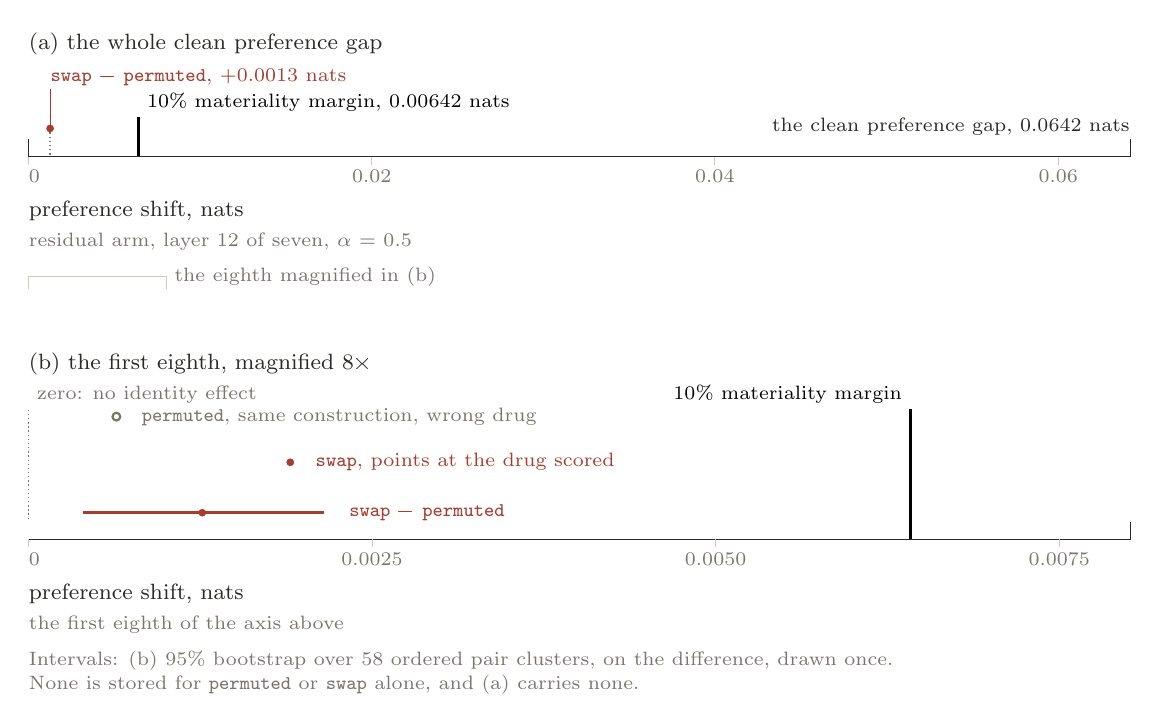
\begin{tikzpicture}[x=1cm, y=1cm, font=\small, inner ysep=1pt, inner xsep=0pt,
  %% TYPE. Two sizes above 7pt and one face (S1, W12). \footnotesize = 10.0pt
  %% carries the two panel heads and the two axis-label line ones and nothing
  %% else; \scriptsize = 8.0pt carries ticks, direct labels, scope lines, the
  %% threshold labels and the interval declaration. No sans, no bold, no italic.
  %% INNER SEP, PASS 10 (X12). It was inner sep = 1pt on the whole picture; the
  %% vertical half is unchanged, so every clearance below is still box
  %% arithmetic, but the horizontal half is now 0pt. With xsep = 1pt every
  %% left-anchored text box stood 1.19pt (0.42mm) inside the axis's left end,
  %% so both rules protruded to the left of the entire text column and S5's
  %% "left-aligned to the axis's left end" was met to 0.42mm and not exactly.
  head/.style  ={font=\footnotesize, text=ink,      anchor=base west},
  axlab/.style ={font=\footnotesize, text=ink,      anchor=base west},
  scope/.style ={font=\scriptsize,   text=quietink, anchor=base west},
  qlabz/.style ={font=\scriptsize,   text=quietink, anchor=base west},
  lab/.style   ={font=\scriptsize,   text=ink,      anchor=base west},
  labR/.style  ={font=\scriptsize,   text=ink,      anchor=base east},
  acc/.style   ={font=\scriptsize,   text=accent,   anchor=base west},
  rowq/.style  ={font=\scriptsize,   text=quietink, anchor=west},
  rowa/.style  ={font=\scriptsize,   text=accent,   anchor=west},
  %% Tick numerals are INK, not quietink: they are part of the axis, and S8
  %% gives ink to axes and axis labels while quietink means a comparator or a
  %% control. 4.11 and 4.13 both set their tick numerals dark for this reason.
  num/.style   ={font=\scriptsize,   text=quietink, anchor=north,
                 inner sep=0pt},
  numL/.style  ={font=\scriptsize,   text=quietink, anchor=north west,
                 inner sep=0pt},
  blab/.style  ={font=\scriptsize,   text=black,    anchor=base west},
  blabR/.style ={font=\scriptsize,   text=black,    anchor=base east},
  %% FIVE STROKE WEIGHTS, each with one meaning (S10, W11).
  tick/.style  ={rulegrey, line width=0.3pt},                  % furniture
  lead/.style  ={rulegrey, line width=0.3pt},                  % furniture
  accled/.style={accent,   line width=0.3pt},                  % furniture, in the mark's colour (S22)
  spine/.style ={ink,      line width=0.4pt},                  % axis rule and its two end caps
  proj/.style  ={quietink, line width=0.5pt, densely dotted},  % zero rule / projection (S7)
  thresh/.style={black,    line width=0.9pt},                  % the one threshold (S6, W3)
  bar/.style   ={accent,   line width=1.0pt},                  % interval
  ctrl/.style  ={quietink, line width=0.8pt}]                  % open-disc edge: a MARK edge, not a rule (S9, W11)

  %% ==== THE TWO MAPS ====================================================
  %% Superseded constants, kept in materiality.json: 0.55+(#1)*207.1650 and
  %% 0.55+(#1)*1657.3200. The 0.55cm inset is gone so that the axis's left end
  %% and the panel's x origin are one coordinate (S13, W1).
  %% 1744.0000 = 8 x 218.0000 EXACTLY, so the magnification is exactly eight,
  %% and \ga{clean_ab_gap} = \gb{clean_ab_gap/8} = 13.995613cm exactly.
  %% PASS 10, X1: the pass-9 header block records these two constants as
  %% 215.7500 and 1726.0000 and the shared right end as 13.851163cm. Those
  %% numbers were never drawn by this file. The two lines below are the map,
  %% and materiality.json has always recorded them correctly.
  \def\ga#1{{(#1)*218.0000}}   % band (a): 0 .. 0.06420005919957501 nats
  \def\gb#1{{(#1)*1744.0000}}  % band (b): 0 .. 0.008025007399946877 nats

  %% ==================== BAND (a) -- THE WHOLE GAP ========================
  %% PASS 11, Y1: the head names the object by the registry string. It read
  %% "(a) the whole preference gap" while the terminal label 8cm to its right
  %% read "the clean preference gap", so one JSON key (clean_ab_gap) carried
  %% two names inside one panel, which is what S19's mechanical check forbids.
  %% "whole" is kept because it is the contrast with (b)'s "first eighth".
  \node[head] at (0.00,9.90) {(a) the whole clean preference gap};

  % The estimate, drawn once and without a bar (W6). At true scale it stands
  % 2.75mm from the origin on a 139.96mm rule, which is the panel's whole point.
  % Its name is band (b) row three's name, because one JSON key takes one name.
  % PASS 10, X4: THE LABEL IS ANCHORED AT THE MARK, not at the panel origin.
  % Pass 9 set it base west on x = 0.00 while its leader fell from
  % \ga{diff_perm} = 0.2751, so the leader descended from inside the word
  % "swap" and the mark read as the SWAP arm -- whose value is 0.0019, not the
  % 0.0013 drawn. That is the one mark in band (a); mis-naming it loses the
  % panel. The label now begins on the mark's own x, and the leader falls from
  % its first character.
  % PASS 11, Y2: THE LABEL PRINTS THE VALUE, AND IT DROPPED 0.06cm.
  % Two defects, one edit. (i) At 9.56 the label stood 0.34cm under the panel
  % head, near-left-aligned with it (7.8pt of indent), so head and label read
  % as a two-line title and the panel's single mark lost its name; the head's
  % descenders cleared the label's ascenders by 2.6pt. At 9.50 that clearance
  % is 4.3pt and the gap to the threshold label below is 0.34cm = 9.7pt, which
  % is still wider than the 7.94pt X6(i) condemned. (ii) Without a value the
  % math minus between two mono tokens parses as easily as a gloss dash --
  % "swap, that is, permuted" -- so the one mark in (a) could be read as the
  % SWAP arm, whose value is 0.0019 and not the 0.0013 drawn. The value now
  % settles it, and it also makes (a) self-sufficient for the figure's
  % question: 0.0013 against the 0.0642 printed at the axis's right end, and
  % against the 0.00642 printed at the threshold.
  % WHY A VALUE MAY BE PRINTED HERE AND NOT ON A ROW OF (b). This label sits
  % 0.96cm above the spine and is leadered to its disc; positions in that lane
  % are not read as values, which is why (a)'s threshold label already prints
  % 0.00642 three centimetres right of the rule it names and its terminal
  % label prints 0.0642 four centimetres left of the cap it names. A label set
  % on a data row's OWN baseline is read positionally, which is why the value
  % came off (b)'s row three (Y8).
  \node[acc] at (\ga{0.0012618344965644142},9.50)
    {\texttt{swap} \textminus{} \texttt{permuted}, +0.0013 nats};
  % The label's leader is accent 0.30pt, the mark's own colour (S22). PASS 10,
  % X5: it now LANDS ON THE DISC. It used to stop at 9.12 against a disc whose
  % top edge is 8.9493, leaving 4.84pt of white, so the leader read as a stray
  % accent tick under the label and the label read as unattached.
  \draw[accled] (\ga{0.0012618344965644142},9.40)
             -- (\ga{0.0012618344965644142},8.95);
  % The stem down onto the spine anchors the mark to a coordinate rather than
  % leaving it floating above the rule; pass 8 added it after both reviewers
  % reported they could not tell whether the mark was a mark, a tick or a
  % printing artefact, and it survives the rebuild. It is drawn in the PROJECTION
  % register -- quietink 0.5pt densely dotted, which is what S7 reserves that
  % stroke for -- and not in the leader's accent, because on the build that drew
  % leader and stem at one weight and one colour the assembly read as a VERTICAL
  % interval bar with a dot on it, which is the one thing this figure must not
  % appear to draw. PASS 10, X5: it now touches the disc's lower edge (8.85
  % against the disc's 8.8507) and the spine (8.54), instead of floating 2.0pt
  % clear of the one and 0.57pt clear of the other.
  \draw[proj] (\ga{0.0012618344965644142},8.85)
           -- (\ga{0.0012618344965644142},8.54);
  \fill[accent] (\ga{0.0012618344965644142},8.90) circle (1.4pt);

  % The one threshold, black and solid, in both bands (S6, CF2, W3). Its value
  % is printed here and the quantity it is a tenth of is printed at the axis's
  % right end, so the tenth is a division on two printed numbers and needs no
  % brace (W5).
  % PASS 10, X3: IT STANDS ON THE SPINE AND NO LONGER CROSSES IT. Pass 9 drew
  % it from 8.38, which is 0.06cm BELOW the hanging ticks' ends and 0.02cm above
  % the tick numerals, so the heaviest stroke in the panel doubled as an
  % outsized unnumbered tick sitting between the numerals "0" and "0.02" -- the
  % same "the threshold merges with the tick furniture" defect S7 indicts in
  % fig:comparators row (a). Band (b) already drew its half of the same
  % threshold from its own spine upward; the two now agree.
  \draw[thresh] (\ga{0.006420005919957502},8.54)
             -- (\ga{0.006420005919957502},9.04);
  \node[blab] at (1.50,9.16) {10\% materiality margin, 0.00642 nats};

  % The axis. PASS 10, X7: BOTH ENDS NOW CARRY THE SAME CAP. The right end is
  % the clean preference gap and has always carried a rising 0.22cm ink stub;
  % the left end carried only the same rulegrey hanging tick as 0.02, 0.04 and
  % 0.06, so the span whose full width IS the figure's denominator was
  % delimited at one end by an ink stub and at the other by an ordinary tick,
  % and did not read as a bounded span at all. Two matching caps, no new weight
  % and no new colour.
  % PASS 11, Y3: THE AXIS'S RIGHT END IS COMPUTED, NOT TRANSCRIBED. It was
  % hard-coded 13.995613 here, at the end cap and at the terminal label, while
  % W1 and the layout note both assert that "every data x is still computed
  % inside pgfmath from the full-precision float, so no value is rounded into
  % the source". \ga{0.06420005919957501} = 13.995612905507352, so the literal
  % was short by 3.5e-7cm -- invisible, but it is the ONE coordinate this
  % figure exists to draw, and the claim about it was false. Only the pinned
  % bounding box below still carries a rounded literal, and it carries no
  % value: it is a box corner, declared as such at Y13.
  \draw[spine] (0.00,8.54) -- (\ga{0.06420005919957501},8.54);
  \draw[spine] (0.00,8.54) -- (0.00,8.76);
  \draw[spine] (\ga{0.06420005919957501},8.54) -- (\ga{0.06420005919957501},8.76);
  % PASS 10, X6: the terminal label sits ON ITS OWN CAP, at y = 8.86, and no
  % longer shares the 9.16 baseline and the "<name>, <value> nats" construction
  % with the threshold label 8cm to its left. Read cold on the pass-9 build the
  % two were one row of two labels in one style, so "the clean preference gap,
  % 0.0642 nats" read as the label of a RULE and a reader looked for a rule at
  % 0.0642 and found a 0.22cm end cap. It is now 0.10cm above that cap.
  \node[labR] at (\ga{0.06420005919957501},8.86)
    {the clean preference gap, 0.0642 nats};
  \foreach \v/\t in {0.02/0.02, 0.04/0.04, 0.06/0.06}{
    \draw[tick] (\ga{\v},8.54) -- (\ga{\v},8.44);
    \node[num] at (\ga{\v},8.38) {\t};}
  % Zero is both the axis's left end and the panel's x origin, so its numeral is
  % set flush with that origin rather than centred on it: a centred "0" is the
  % only object that would break the figure's single left edge (S13).
  \draw[tick]  (0.00,8.54) -- (0.00,8.44);
  \node[numL] at (0.00,8.38) {0};

  % AXIS LABEL, in axis-label position: directly under the tick numerals, left
  % edge on the axis's left end, quantity and unit on line one (S5, W2).
  % PASS 10, X13: set lowercase, as 4.11 and 4.13 set every axis label of
  % theirs and as S19's registry gives the name.
  % PASS 11, Y4: THE SCOPE LINE DROPS 0.12cm AND DISCLOSES THE SELECTION.
  % (i) LEADING. It was set 0.28cm under a 9.96pt line, which is 7.94pt of
  % baseline-to-baseline for type 2pt larger than the lead -- negative leading,
  % and the tightest of the four stacked pairs in this figure. Four such pairs
  % were set at or under solid and it is the single thing that made the figure
  % look crowded beside 4.11. Both axis-label blocks and the foot block now
  % open to 0.38cm (10.8pt), and the whole of the added height was paid for out
  % of the white between the two bands, which fell 1.14cm -> 0.77cm.
  % (ii) SELECTION. "layer 12" alone is a scope statement. Layer 12 is the
  % argmax of the anchor seed's seven-depth sweep and the only one of the seven
  % whose interval excludes zero (diff_perm_norm with p_perm: +0.0022 p 0.583,
  % -0.0050 p 0.139, -0.0025 p 0.4495, +0.0041 p 0.3955, -0.0019 p 0.635,
  % +0.0197 p 0.001, +0.0059 p 0.4885 at layers 2/4/6/8/9/12/16). "of seven"
  % is nine characters and it tells a reader on the drawing that the depth was
  % one of a set; WHICH one, and why that matters, is caption material and the
  % proposed caption in figs/_PENDING_CAPTIONS.tex carries it. Until a human
  % integrates that caption the printed one (04b:617-618) says only "one arm at
  % one depth at one rung", which is scope and not selection.
  \node[axlab] at (0.00,7.78) {preference shift, nats};
  \node[scope] at (0.00,7.40)
    {residual arm, layer 12 of seven, $\alpha$ = 0.5};

  % The magnified span, named as an object and not traced by a leader (W10).
  % Its two stubs turn DOWN, towards the panel that opens the span, so the
  % bracket points at (b) instead of back at an axis it already stands under.
  % PASS 10, X8: raised 0.16cm, tight under the scope line, and its label now
  % NAMES the object as well as pointing at (b). Two reviewers asked for it to
  % be moved into the lane immediately under the tick numerals with its stubs
  % reversed; both halves of that were overruled, and the reason is recorded in
  % the pass-10 block under X8.
  % PASS 11, Y5: THE STUBS ARE LONG ENOUGH TO SEE, AND THE BRACKET STANDS
  % CLEAR OF THE AXIS-LABEL BLOCK. Measured on the pass-10 render, each stub
  % was 4 pixels at 200dpi -- 1.44pt, 0.51mm -- of 0.30pt rulegrey, which does
  % not survive print, so the assembly was a bare grey horizontal sitting
  % 0.34cm under a scope line that runs past both of its ends: it read as an
  % underline of "residual arm, layer 12," or as an editorial divider, and not
  % as a bracket. Two changes, no new weight and no new colour: the stubs go
  % 0.06cm -> 0.16cm, and the gap from the scope line goes 0.34cm -> 0.44cm,
  % which is larger than the 0.38cm internal leading of the axis-label block
  % above it, so the bracket stops reading as that block's third line.
  % Two harder proposals were overruled and the reasons are at Y15 (c) and (d).
  \draw[lead] (0.00,6.86) -- (0.00,7.02)
           -- (\ga{0.008025007399946877},7.02)
           -- (\ga{0.008025007399946877},6.86);
  \node[scope] at (1.85,6.96) {the eighth magnified in (b)};

  %% ============= BAND (b) -- THE FIRST EIGHTH, MAGNIFIED =================
  %% PASS 11: the whole of band (b) is raised 0.14cm and its axis lowered
  %% 0.10cm, which is where the leading opened at Y4 and Y11 was paid from.
  \node[head] at (0.00,5.84) {(b) the first eighth, magnified 8\texttimes{}};
  % The threshold label sits against the rule it names and takes the LEFT of it
  % here and the RIGHT of it in (a): in each band the label goes on the side
  % where the rule has room, which in (a) -- where the rule stands at a tenth of
  % the measure -- is the right, and in (b) -- where it stands at four fifths --
  % is the left. Set right of the rule here it measures 2.98cm from 11.30 and
  % crosses the right end of the axis at 13.996 (checked on a build, which
  % reported Overfull \hbox 2.84pt).
  % PASS 10, X6: it has come off the panel head's baseline (5.70) and down onto
  % its own, 0.12cm above the rule's top, in the same relation to its rule as
  % (a)'s label is to (a)'s. On the pass-9 build it sat at exactly the head's
  % baseline, so scanning the two panel heads read "(b) the first eighth,
  % magnified 8x ... 10% materiality margin" as one title line.
  \node[blabR] at (11.10,5.46) {10\% materiality margin};
  \draw[thresh] (\gb{0.006420005919957502},3.68)
             -- (\gb{0.006420005919957502},5.34);

  % Zero. Densely dotted quietink 0.5pt is this document's stroke for a
  % coordinate that decides nothing (S7).
  % PASS 11, Y6: IT IS NAMED, ON THE SAME BASELINE AS THE THRESHOLD LABEL AND
  % AT THE SAME 0.12cm ABOVE ITS OWN RULE'S TOP. SUPERSEDES W8's closing
  % clause, that the rule "carries no label, because its foot is the axis's own
  % 0 numeral". The equivalence criterion of 04b:507-513 is a CONJUNCTION --
  % the interval must lie inside the margin AND contain zero -- and this
  % figure's result is that it does the first and not the second. Pass 10 drew
  % the margin conjunct as the heaviest stroke on the page and the zero
  % conjunct as an unlabelled 0.5pt dotted rule standing on the panel's own x
  % origin, where it has no figure/ground of its own; at a 4x squint it
  % disappeared entirely. Naming it is what the figure's spec authorises ("if
  % the zero rule needs a name it takes 'zero' in \scriptsize roman ink at the
  % rule") and it is the whole of the fix: the rule is NOT promoted to the
  % threshold register, because S6 reserves black solid 0.90pt for a threshold
  % and S7 reserves this stroke for a coordinate that decides nothing -- which
  % zero, as a coordinate, is. What decides is whether the bar clears it, and
  % the bar clears it by 0.70cm.
  % The label is placed with an xshift on the rule's own x, as the row labels
  % are placed on their marks', so it is tied to the thing it names; the two
  % vertical rules of (b) now carry one \scriptsize label each, on one
  % baseline, one at each rule's top (S22).
  % PASS 10, X9: it no longer starts on the spine. Drawn 3.58 to 5.56 it was
  % collinear and continuous with the axis's left terminus, its hanging tick and
  % the panel's x origin, ran the full height of the data region, and matched
  % the threshold rule on the right for length -- so all three reviewers read
  % the pair as the two sides of a frame round the rows, which is the object
  % S12 exists to forbid. It now spans the three rows only, 0.28cm clear of the
  % spine and 0.42cm clear of the panel head, and reads as what it is: the
  % coordinate the interval bar's left end clears by 0.70cm.
  \draw[proj] (0.00,3.94) -- (0.00,5.34);
  \node[qlabz, xshift=3pt] at (0.00,5.46) {zero: no identity effect};

  % ROW ONE, the control: an open disc, white fill, 0.8pt quietink edge, which
  % is 4.11's own encoding for a comparator or a null (S9, CF5, W11).
  % PASS 10, X10: the gloss separator is a comma. It was an em dash, in the same
  % position after the token as row three's math minus, so one glyph class
  % carried "namely" in two rows and "subtract" in the third on a figure whose
  % whole subject is a subtraction. The minus in row three and in band (a) is
  % now the only dash inside a label anywhere on the drawing.
  % X12: the three row labels are placed with an xshift on the mark's own
  % coordinate rather than at a literal x, so each label is tied to its mark.
  % PASS 11, Y7: THE MARK-TO-LABEL GAP GOES 5pt -> 9pt IN ALL THREE ROWS.
  % SUPERSEDES X12's closing clause, which set it at 5pt. At 5pt the open
  % control disc stood 3.28pt from the first glyph of \texttt{permuted}, which
  % is LESS than Inconsolata's own character advance at this size (3.43pt),
  % while its outer diameter (3.6pt) is 11% larger than that face's x-height
  % (3.24pt measured at 200dpi) and its 0.80pt edge is of comparable weight to
  % the stems beside it. The one comparator mark on the drawing therefore set
  % as a lowercase letter o prefixing the word: at 12x it reads "o permuted".
  % Row two escaped only because its disc is filled and accent. At 9pt the gap
  % is 7.2pt, twice the mono advance, and the ring is a mark again.
  % A second fix was proposed for the same defect -- take the ring's edge to
  % ink, as 4.11(b) does -- and it is overruled at Y15 (a).
  \fill[white]  (\gb{0.0006409306049362111},5.24) circle (1.4pt);
  \draw[ctrl]   (\gb{0.0006409306049362111},5.24) circle (1.4pt);
  \node[rowq, xshift=9pt] at (\gb{0.0006409306049362111},5.24)
    {\texttt{permuted}, same construction, wrong drug};

  % ROW TWO, the arm under test.
  \fill[accent] (\gb{0.0019027651015006252},4.66) circle (1.4pt);
  \node[rowa, xshift=9pt] at (\gb{0.0019027651015006252},4.66)
    {\texttt{swap}, points at the drug scored};

  % ROW THREE, the measurement, and the only interval on the figure. The label
  % is anchored on the interval's upper end, which is the rightmost ink in the
  % row, so it clears the bar by the same 9pt the other two clear their discs.
  % PASS 11, Y8: THE VALUE COMES OFF THIS LABEL. It printed "$+0.0013$ nats"
  % 48.9pt (17.2mm) to the right of the disc whose value it is, ON THE ROW'S
  % OWN BASELINE, where position is value: the numeral stood at x = 0.00339 on
  % (b)'s axis, 2.7 times the number it printed and past the 0.0025 tick, on
  % the one panel whose job is to let a reader place the estimate between zero
  % and the 0.00642 margin. Rows one and two anchor at their marks and this
  % row anchored at its bar's end, so one panel carried two anchoring rules and
  % the one that misplaced its label was the one that printed a number. The
  % label is now the row's NAME only, which is the same string band (a) uses
  % for the same JSON key (S19), and the value is printed once, in (a), at a
  % label lifted off the data lane and leadered to its disc (Y2). After this
  % edit no numeral anywhere on the drawing stands on a data row's baseline.
  % PASS 11, Y9: 0.06cm MORE AIR UNDER ROW TWO. The bar on this row spans
  % 0.702 to 3.751cm and the two arm marks stand at 1.118 and 3.318, so the
  % interval on the DIFFERENCE horizontally contains both of its own operands
  % and the difference disc falls within 0.02cm of their midpoint by
  % arithmetic accident. A reader can be offered "a 95% interval that brackets
  % both arms", which is the opposite of what the row says. The row pitch is
  % now 0.58 / 0.64 rather than a flat 0.54, so the derived row sits off the
  % pair it is derived from; the label states the derivation; and the proposal
  % to delete the two arm marks outright is overruled at Y15 (b).
  \draw[bar] (\gb{0.0004024989353392094},4.02)
          -- (\gb{0.002150955667015771},4.02);
  \fill[accent] (\gb{0.0012618344965644142},4.02) circle (1.4pt);
  \node[rowa, xshift=9pt] at (\gb{0.002150955667015771},4.02)
    {\texttt{swap} \textminus{} \texttt{permuted}};

  % The magnified axis, its ticks landing on the same four x as band (a)'s so
  % that the two rules read as one rule at two scales (W13).
  % PASS 11, Y10: BAND (b) IS CAPPED AT ITS RIGHT END, AND ITS END IS COMPUTED.
  % SUPERSEDES W13's closing clause ("band two's right endpoint ... takes no
  % tick and no numeral"). W13 declined a terminal MARK on the ground that
  % (b)'s right end is named by (b)'s axis label rather than by a mark, and
  % that reasoning stands -- but what it left was 26.01pt (9.17mm) of bare
  % rule running past the last drawn tick to an end with nothing on it, which
  % is the same rule-end-to-last-tick defect S13 measures at 8.1mm in
  % fig:comparators row (c). Band (a) has the identical overhang and closes it
  % with a 0.22cm ink cap; band (b) now closes it with the same cap, at the
  % same x, in the same weight and colour, so the two rules terminate
  % identically at the end where the overhang is and read as one rule at two
  % scales. The cap is axis furniture -- the rule's own end -- and not a data
  % mark, so S20 is untouched; the proposal to hang a value on it is overruled
  % at Y15 (e). NO LEFT cap is added in (b): a 0.22cm ink stub rising from the
  % spine at x = 0 would stand 0.14cm under the dotted zero rule and collinear
  % with it, which is exactly the frame-edge reading X9 removed.
  \draw[spine] (0.00,3.68) -- (\gb{0.008025007399946877},3.68);
  \draw[spine] (\gb{0.008025007399946877},3.68)
            -- (\gb{0.008025007399946877},3.90);
  % PASS 11, Y11: the middle numeral prints 0.0050 and not 0.005. Band (a)'s
  % three numerals carry two decimals each and band (b)'s carry four, and the
  % one visible proof that (b) is (a) divided by eight is that the two lanes
  % put congruent numerals on the same four x. A dropped place broke the
  % column of trailing digits that carries it. The VALUE is unchanged; this is
  % a print string, which is why the \foreach takes the value/label pair form.
  \foreach \v/\t in {0.0025/0.0025, 0.005/0.0050, 0.0075/0.0075}{
    \draw[tick] (\gb{\v},3.68) -- (\gb{\v},3.58);
    \node[num] at (\gb{\v},3.52) {\t};}
  \draw[tick]  (0.00,3.68) -- (0.00,3.58);
  \node[numL] at (0.00,3.52) {0};

  \node[axlab] at (0.00,2.92) {preference shift, nats};
  % PASS 10, X14: "magnified 8x" comes off this line. The panel head 3.2cm
  % above already carries it, and the exactness of the eight is caption
  % material; what the axis-label line has to carry is the relation to the axis
  % above, which is what is left.
  \node[scope] at (0.00,2.54) {the first eighth of the axis above};

  %% ==== THE ONE INTERVAL DECLARATION, at the foot (S17, CF8) =============
  %% PASS 10, X2. The pass-9 second line read "No interval is returned for
  %% permuted, for swap, or for (a)." That was false, and false about the one
  %% mark on the figure that does have an interval: band (a)'s disc IS
  %% diff_perm, and layers.12.swap.ci_perm is an interval on diff_perm. In this
  %% document "returned" is what the instrument does, so the sentence told a
  %% reader that band (a)'s estimate has no uncertainty available and, by
  %% implication, that (a) and (b) draw different quantities. The declaration
  %% now separates non-existence from non-drawing: the arms have no stored
  %% interval, the difference has one, and it is drawn once.
  %% Leading is 0.28cm here, as everywhere else in this figure. At pass 9 the
  %% two lines were set 0.24cm apart, tighter than solid for 8pt type, and the
  %% descender of "bootstrap" met the dot of the "i" below it.
  %% PASS 11, Y12: 0.28cm -> 0.30cm between the two lines, and 0.46cm from the
  %% axis-label block above rather than 0.42cm. 0.28cm is exactly solid for
  %% 7.97pt type and the two lines' boxes met; the block also has to stand off
  %% the axis-label block by more than that block's own 0.38cm internal
  %% leading, or the four lines read as one four-line paragraph.
  %% PASS 11: six characters come out of these two lines, and nothing else, to
  %% keep the figure under S15's 5.0 characters per 100mm^2 after "of seven",
  %% "clean" and "zero" went in. Both sentences say exactly what they said.
  \node[scope] at (0.00,2.08) {Intervals: (b) 95\% bootstrap over 58 ordered pair clusters, on the difference, drawn once.};
  \node[scope] at (0.00,1.78) {None is stored for \texttt{permuted} or \texttt{swap} alone, and (a) carries none.};

  % The bounding box IS the body block; nothing may stick out of it.
  % PASS 11, Y13: the floor goes 1.72 -> 1.68 to keep the foot block's
  % descenders inside. This \path is the one rounded literal left in the file
  % and it carries no value: 13.9957 is a box corner, not a coordinate any
  % mark is drawn at, and every data x is computed by \ga or \gb from the
  % full-precision float (Y3).
  \path (0.00,1.68) rectangle (13.9957,10.18);
\end{tikzpicture}
%
% ---------------------------------------------------------------------------
% READY TO PASTE into Sections/04b-representation.tex, at sec:res-mechanism,
% immediately after the verdict paragraph (04b:332-342) or, if the page breaks
% badly, after the equivalence-criterion paragraph (04b:412-419). The same block
% was staged, at pass 9, in a figs/_PENDING_FLOATS.tex that does not exist;
% PASS 10 supersedes that: the float wrapper is HERE and the caption is in
% figs/_PENDING_CAPTIONS.tex, which does exist as of this pass (X15).
%
% PASS 9 NOTE. The caption below is the PROPOSED replacement and it is not yet
% in Sections/. No builder on this pass may edit Sections/04b-representation.tex,
% so the same text is written into figs/_PENDING_CAPTIONS.tex keyed by
% \label{fig:materiality} for a human to integrate. Until that happens the
% caption printed in main.pdf is the pass-8 one, and three of its clauses are
% false of the rebuilt drawing -- see CAPTION NOTE, PASS 9 at the foot.
%
% \begin{figure}[htbp]
% \centering
% \input{figs/materiality}
% \caption[The effect and its gap]{\captiontitle{The model
% does move its preference towards the other drug's own held-out sentence, but
% by one fiftieth of the preference it already has and one fifth of the margin
% set in advance.} Residual arm, layer $12$, $\alpha = 0.5$, from
% \texttt{probe\_arm\_residual.json}; normalised, the same estimate is the
% \ci{+0.0197}{+0.0063}{+0.0335} of \cref{tab:identity} and
% \cref{fig:comparators} row (c). \emph{(a)} The model's clean preference gap
% between the two sentences compared, measured with no intervention and drawn
% end to end between two ink caps, so that the axis's full width is the
% denominator every effect in this section is divided by; the effect is the
% accent disc near the origin, named at itself and dotted down onto the rule,
% and the bracket below the axis label marks the eighth of the gap that (b)
% opens out. \emph{(b)} That first eighth at exactly $8\times$ --- exactly,
% because the lower scale is the upper one divided by eight and not by a
% rounded number --- in the same units, where the \texttt{permuted} control at
% $0.00064$ nats, the \texttt{swap} arm at $0.00190$ and their difference,
% $+0.0013$, separate; the difference is the only one of the three this thesis
% quotes anywhere. The black rule in both panels is the $10\%$ materiality
% margin pre-registered for calling an effect material, drawn in the same
% weight and colour as in \cref{fig:family} and \cref{fig:comparators} row (c).
% \textbf{Which bootstrap draw this is.} The bar is
% \texttt{layers.12.swap.ci\_perm}, the top-level draw, $p = 0.001$ over a
% $4000$-resample cluster bootstrap on $60$ rows in $58$ pair clusters over
% $24$ anchor drugs. The arm's file stores a second draw of the same point
% estimate inside the $\alpha = 0.5$ rung of the ladder, at $p = 0.004$, and
% \cref{fig:family}'s lower strip draws that one; the two lie either side of
% the $0.05/26$ admitted at rank one, so the choice decides whether anything in
% the family survives multiplicity correction. This figure quotes the top-level
% draw because \cref{tab:identity}, \cref{fig:comparators} row (c) and the
% correction itself all rest on it. \textbf{What the interval shows, and what
% it does not.} It excludes zero \emph{and} lies wholly inside the margin:
% under textbook TOST that configuration is returned as equivalence and read as
% a null, whereas this chapter's rule returns a directional effect smaller than
% the margin --- one fiftieth of the gap, one fifth of the margin.
% \textbf{No interval is drawn on the two arms or in (a).} None is stored for
% \texttt{effect\_swap} or \texttt{effect\_perm} alone, so their marks are bare;
% the one that is stored is on their difference, which is (a)'s single mark as
% well as (b)'s third row, and it is drawn once, at the scale where it is
% legible. What may not be read across: layer $12$ is one of seven
% pre-registered depths and the only one whose interval excludes zero, the
% other six being in \cref{fig:family}'s grid, and this is one arm at one depth
% at one rung of the displacement ladder; because the five arms emit different
% target formats their clean gaps run from this arm's $0.064$ nats to $0.314$
% in the consensus arm, nearly fivefold, so a raw-nats axis is legitimate here
% and nowhere across arms --- \cref{fig:family}'s lower strip is a single-arm
% object for the same reason.}
% \label{fig:materiality}
% \end{figure}
%
% CAPTION NOTE, PASS 10. The pass-9 note below is kept; these are the further
% changes this pass made, and the reason for each.
%   * "the accent mark ... labelled there" became "named at itself", because at
%     pass 9 the label was anchored on the PANEL origin and not on the mark, so
%     the caption's claim was false of the drawing (X4). It is true now.
%   * "drawn end to end" gained "between two ink caps", because the span now
%     has two matching end caps and the caption should name the device that
%     makes the axis read as a bounded span (X7).
%   * THE TWO OPERANDS ARE PRINTED: the permuted control at 0.00064 nats and
%     the swap arm at 0.00190, rounded from effect_perm 0.0006409306049362111
%     and effect_swap 0.0019027651015006252. Band (b) draws them as positions
%     and prints neither, and the subtraction they stand in is the reason both
%     rows exist; a reader could previously check it only by measuring three
%     rows with a ruler. Both are new readings quoted in no sentence of the
%     thesis, which the ledger has always recorded, so the caption owns them --
%     and it now says so by naming the difference as the only one of the three
%     the thesis quotes.
%   * LAYER 12 IS DISCLOSED AS THE FAVOURABLE DEPTH: "one of seven
%     pre-registered depths and the only one whose interval excludes zero".
%     Recomputed from probe_arm_residual.json layers.<L>.swap.diff_perm_norm
%     and p_perm: +0.0022 p 0.583 (L2), -0.0050 p 0.139 (L4), -0.0025 p 0.4495
%     (L6), +0.0041 p 0.3955 (L8), -0.0019 p 0.635 (L9), +0.0197 p 0.001 (L12),
%     +0.0059 p 0.4885 (L16); six of seven ci_perm_norm straddle zero.
%     fig:hook's caption discloses its layer 4 as the best of seven and this one
%     did not, though "surviving" in this figure's own subject is doing exactly
%     that selection work. The RUNG is not favourable and is not flagged: in raw
%     nats alpha = 0.5 gives the smallest of the five ladder effects (0.0013
%     against 0.0017 / 0.0044 / 0.0061 / 0.0046), so the drawn rung is the
%     conservative one.
%   * "separate into three rows" -- pass 9 cut "into three rows"; the phrase
%     stays cut, since the rows still carry no dividers.
%   * The pass-9 caption is otherwise unchanged, and it is now WRITTEN OUT, in
%     full and uncommented, in figs/_PENDING_CAPTIONS.tex keyed by
%     \label{fig:materiality}, together with the two sentences deleted from the
%     drawing at W9 and a list of the clauses of the caption PRINTED today
%     (Sections/04b-representation.tex:597-620) that the rebuild made false.
%     At pass 9 that file was asserted to exist and did not (X15).
%
% CAPTION NOTE, PASS 9. What changed, and why each clause had to.
%   * "the effect is the accent mark near its origin, stemmed to the axis and
%     labelled there, and the brace under it marks the eighth ..." became
%     "the accent disc ... dotted down onto the rule ... and the bracket beneath
%     the axis marks the eighth ...". The mark is a disc and no longer a bar
%     (W6), the stem is now a dotted projection and not an accent stem (W11),
%     and the magnifier is a bracket and not a brace (W10).
%   * "only their difference does, and it is the one bar on the figure" became a
%     bolded sentence of its own, because at pass 8 the caption said one bar and
%     the drawing showed two -- the same estimate at two magnifications -- and a
%     naive reader counted them and had to work out which two quantities they
%     were. There is now exactly one bar and the caption says where it is.
%   * "separate into three rows" lost "into three rows": the rows no longer carry
%     dividers, so there is nothing to count (W5).
%   * WHICH BOOTSTRAP DRAW IS DRAWN is new, and it is the substantive addition.
%     4.12 and 4.13's lower strip draw the identical point estimate
%     0.0012618344965644142 in identical units and visibly identical bars, from
%     two different bootstrap draws with p = 0.001 and p = 0.004, and neither
%     drawing said so. Both ledgers knew (materiality.json's
%     not_drawn_second_bootstrap_draw; family.json's ladder note), so this was a
%     disclosure failure on the page and not a data error.
%   * THE TOST ASYMMETRY moved here in full from the drawing (W9), where it was
%     two ink lines at 8pt that a reader met before the real caption. It is the
%     section's subtlest point and it is argument, so it belongs here.
%   * "one fiftieth of the gap; one fifth of the margin" moved here from the
%     drawing's accent italic (W9). It was already the caption's lede in
%     substance; it now appears once.
%   * THE $10\%$ MARGIN's rendering is named, because this is the first build in
%     which 4.7 row (c), 4.12 and 4.13 draw one pre-registered threshold one way.
% ---------------------------------------------------------------------------
%
% ---------------------------------------------------------------------------
% CAPTION NOTE, PASS 11 -- 2026-08-19. THE COMMENTED \caption ABOVE IS THE
% PASS-10 TEXT AND IS NO LONGER THE PROPOSAL. It is left in place because the
% passes above are the audit trail and because the float wrapper round it is
% still the one to paste; the AUTHORITATIVE caption is the one in
% figs/_PENDING_CAPTIONS.tex under \label{fig:materiality}, revised in this
% pass with the drawing. Four of its clauses moved, and one item in that file
% is now marked BLOCKING.
%   * (a)'s single mark now PRINTS ITS VALUE on the drawing (Y2), so the
%     caption stops merely naming it and says that panel (a) alone answers the
%     section's question: the disc is labelled with +0.0013, the threshold with
%     0.00642 and the axis's own right end with 0.0642.
%   * (b)'s row three no longer prints a value (Y8), so the caption's "their
%     difference, $+0.0013$" is now the only statement of that numeral for
%     panel (b).
%   * (b)'s rule is capped in ink at its right end as (a)'s is (Y10), and (b)'s
%     zero rule is labelled "zero" (Y6), so the caption's "It excludes zero"
%     now points at a named object rather than at an unlabelled dotted rule.
%   * The panel head reads "(a) the whole CLEAN preference gap" (Y1).
%   * BLOCKING, and it is the one item in the file whose omission changes what
%     the figure claims rather than how it is described: 04b:617-618 says only
%     "this is one arm at one depth at one rung", which is scope. Layer 12 is
%     the argmax of the anchor seed's seven-depth sweep and the only one of the
%     seven whose interval excludes zero. The drawing now says "layer 12 of
%     seven" (Y4) -- that the depth came from a set -- but a drawing cannot say
%     WHICH of the set without becoming an argument. The proposed caption
%     carries it as a bolded clause of its own, with the seven normalised
%     effects and their bootstrap p, and with the countervailing fact that the
%     RUNG is not favourable: at alpha = 0.5 the raw effect is the smallest of
%     the five rungs, 0.0013 against 0.0017, 0.0044, 0.0061 and 0.0046
%     (probe_arm_residual.json :: layers.12.swap.ladder[*].diff_perm).
% ---------------------------------------------------------------------------

\caption[The effect and its gap]{\captiontitle{The model does move its preference
towards the other drug's own held-out sentence, but by one fiftieth of the
preference it already has and one fifth of the margin set in advance.}
Residual arm, layer $12$, $\alpha = 0.5$, from
\texttt{probe\_arm\_residual.json}; normalised, the same estimate is the
\ci{+0.0197}{+0.0063}{+0.0335} of \cref{tab:identity} and
\cref{fig:comparators} row~(c). \emph{(a)} The model's clean preference gap
between the two sentences compared, measured with no intervention, drawn end to
end, so that the axis's full width is the denominator every effect in this
section is divided by; the effect is the accent disc near the origin, dotted
down onto the rule and named above it, and the bracket beneath the axis label
marks the eighth of it that~(b) opens out. \emph{(b)} That first eighth at
exactly $8\times$ --- exactly, because the lower scale is the upper one divided
by eight and not by a rounded number, which is why the two tick lanes fall on
the same four positions --- in the same units, where the \texttt{swap} arm, the
\texttt{permuted} control and their difference separate. The black rule in both
panels is the $10\%$ materiality margin pre-registered for calling an effect
material, drawn in the same weight and colour as in \cref{fig:family} and
\cref{fig:comparators} row~(c). \textbf{Which bootstrap draw this is.} The bar
is \texttt{layers.12.swap.ci\_perm}, the top-level draw, $p = 0.001$ over a
$4000$-resample cluster bootstrap on $60$ rows in $58$ pair clusters over $24$
anchor drugs. The arm's file stores a second draw of the same point estimate
inside the $\alpha = 0.5$ rung of the ladder, at $p = 0.004$, and
\cref{fig:family}'s lower strip draws that one; the two lie either side of the
$0.05/26$ admitted at rank one, so the choice decides whether anything in the
family survives multiplicity correction. This figure quotes the top-level draw
because \cref{tab:identity}, \cref{fig:comparators} row~(c) and the correction
itself all rest on it. \textbf{What the interval shows, and what it does not.}
It excludes zero \emph{and} lies wholly inside the margin: under textbook TOST
that configuration is returned as equivalence and read as a null, whereas this
chapter's rule returns a directional effect smaller than the margin --- one
fiftieth of the gap, one fifth of the margin. \textbf{No interval is drawn on
the two arms or in~(a).} None is stored for \texttt{effect\_swap} or
\texttt{effect\_perm} alone, so their marks are bare; the one stored interval
is on the difference and is drawn at the scale where it is legible, which
is~(b), and nowhere else. What may not be read across: this is one arm at one
depth at one rung of the displacement ladder, and because the five arms emit
different target formats their clean gaps run from this arm's $0.064$ nats to
$0.314$ in the consensus arm, nearly fivefold, so a raw-nats axis is legitimate
here and nowhere across arms --- \cref{fig:family}'s lower strip is a
single-arm object for the same reason.}
\label{fig:materiality}
\end{fullwidth}
\end{figure}

\paragraph{The contrast score} Let $g_A$ and $g_B$ be \emph{measured} cell
sentences --- real transcriptomes of held-out cells treated with drugs $A$ and
$B$, taken from the evaluation data and not produced by the model --- and let
$\textrm{prompt}_A$ be the prompt naming drug $A$.

Scoring a sentence means asking how probable the model finds it, and nothing is
generated to find out. Write $g = (t_1, \ldots, t_T)$ for its tokens. The prompt
and the sentence are concatenated into a single sequence and one forward pass is
run over it. At each position the model emits a distribution over the whole
vocabulary for the next token, and what is recorded is the mass it placed on the
token that actually appears there, given the true tokens before it:
\begin{equation}
  \log P\!\left(g \mid \textrm{prompt}\right) \;=\;
  \frac{1}{T} \sum_{i=1}^{T}
  \log P\!\left(t_i \;\middle|\; \textrm{prompt},\, t_1, \ldots, t_{i-1}\right).
\end{equation}
The conditioning is on the true prefix at every step, never on what the model
would itself have written, so a wrong prediction early does not corrupt the
positions after it; and the model is never required to produce $g$, only to
score it. The result is a per-token mean, comparable across sentences of
different lengths.

The quantity the test scores is the difference between two such readings under
the same prompt,
\begin{equation}
  \Delta \;=\;
  \log P\!\left(g_B \mid \textrm{prompt}_A\right) \;-\;
  \log P\!\left(g_A \mid \textrm{prompt}_A\right),
\end{equation}
that is, how much the model prefers the wrong drug's real response to the right
drug's, under a prompt naming the right one. Any offset uniform across positions
cancels exactly in the subtraction, an inflated normaliser included. What does
not cancel is its state-dependent part, since once $g_A$ and $g_B$ diverge the
two sequences visit different states, and that residue is what the second
injection controls.

\paragraph{Two injections sharing an anchor, scored out of sample} Write $\Pi$
for the orthogonal projector onto the purified slab $V_{\textrm{pure}}$, and
$\mu_c$ for drug $c$'s class mean of \cref{sec:res-used}. The treatment adds
\begin{equation}
  \alpha \, \Pi\!\left(\mu_B - \mu_A\right)
\end{equation}
to the residual stream, displacing the activations from the drug the prompt
names towards the drug whose sentence is being scored. Its control adds
$\alpha\,\Pi(\mu_C - \mu_A)$ for a third drug $C$: same construction, same
anchor at $\mu_A$, matched norm, and a displacement pointing at a drug that has
nothing to do with either sentence in the contrast. The two differ in nothing
but which drug they point at, so the difference between them isolates the
model's preference for $B$'s response attributable to being pushed
\emph{towards $B$} rather than to being pushed at all. The subtraction
$\mu_B - \mu_A$ cancels the global mean exactly, and nothing is ablated, so no
removed term enters either.

Three disjoint slices of cells keep the test out of sample: one fits the
subspaces, one supplies the class means, and a third supplies $g_B$, which
therefore never comes from the rows defining $\mu_B$. Were it otherwise, the
injected vector and the scored sentence would share cells and the test would be
partly circular. Because the training arms emit different target formats, every
effect is reported as a fraction of that model's own clean preference gap,
measured with no displacement applied.

\paragraph{Four guards carry the inference} Each guard exists because one
specific way of being wrong is live here, and each is fixed before the test is
run rather than chosen after seeing it.

\emph{The uncertainty model.} The natural unit to resample is the row, but rows
are not independent here: every row is an ordered pair $(A,B)$, and two rows
sharing a pair share both the injected vector and the scored sentence, so
treating them as separate observations would count the same evidence twice and
narrow the interval accordingly. The bootstrap therefore resamples whole pairs,
not rows.\gloss{cluster bootstrap}{resamples whole $(A,B)$ pairs, so two rows
sharing a pair count once} At the anchor seed's layer $12$ this is $60$ rows in
$58$ pair clusters over $24$ anchor drugs --- close to a row bootstrap, because
few pairs repeat --- and it guards only against sharing within a pair, not
across pairs that happen to share an anchor drug or a target drug.

\emph{The equivalence criterion.} A small interval that contains zero can mean
two different things, and they must not be conflated: the effect is genuinely
absent, or the instrument was too blunt to see it. Two one-sided tests, the
standard remedy, declares equivalence whenever the whole interval falls inside a
margin of practical irrelevance.\gloss{TOST}{two one-sided tests: declares
equivalence when the whole interval lies inside a pre-set margin} That is too
generous here, because an interval can lie inside the margin while sitting
entirely above zero --- a real directional effect, merely a small one, which
TOST would return as a null. This section therefore requires both conditions:
the interval must lie inside a margin pre-registered at $10\%$ of the model's
own clean preference gap, \emph{and} it must contain zero. The conjunction runs
one way only. It can withhold a verdict of equivalence that TOST would grant; it
can never manufacture one.

\emph{The headroom gate.} An intervention that produces no effect proves nothing
if the measurement could not have registered one, which is the same
falsifiability problem the removal gate of \cref{sec:res-used} answers for
ablation. Here it is answered per layer: any depth where the cell-line positive
control shows less than $5\times$ dynamic range is excluded outright, because at
that depth the instrument is saturated and can support neither a positive
verdict nor a null.

\emph{The magnitude ladder.} A single displacement gives a single number, and a
single number cannot distinguish a real effect from a coincidence of scale. If
what the injection moves is genuinely the drug's identity, then displacing
further should move the output further --- the effect should grow with $\alpha$.
The test is therefore repeated at $\alpha \in \{0.5, 1, 2, 5, 10\}$ times the
natural displacement, and a monotone dose--response across those rungs is
pre-registered as what a real effect would look like. This is the guard that
bites.

\paragraph{The result of the experiment}
Assembled, the instrument runs as follows. At a given depth, take an evaluation prompt
naming drug $A$; retrieve the measured cell sentences $g_A$ and $g_B$ from the
held-out slice; score, using $\delta$ as defined above, both under $\textrm{prompt}_A$ with the residual stream
displaced by $\alpha\,\Pi(\mu_B - \mu_A)$, and again with it displaced by the
control $\alpha\,\Pi(\mu_C - \mu_A)$; take the difference of the two contrast
scores; repeat over ordered $(A,B)$ pairs; express the result as a fraction of
that model's clean preference gap; put an interval on it by resampling whole
pairs; and admit the depth only if the cell-line control had the headroom to
register an effect there. Then repeat the whole of it at each rung of the
magnitude ladder(that is for varying values of $\alpha$).

Run that way on the single-cell arm --- the model trained to predict the treated
cell's own sentence, and the arm this chapter has measured throughout --- it
returns nothing at any depth where it could be run. The median effect across the
six admitted depths is $-0.0012$: the wrong sign, and two orders of magnitude
beneath the margin. Displacing the activations towards another drug does not
move what the model emits towards that drug.

The sweep that produced this section's verdict was run on the single-cell arm
alone. After the fact, with all five training arms of \cref{tab:trainconfig} in
hand, the identical intervention was re-run across every one of them at up to
seven depths each --- twenty-six measured tests in all, drawn in
\cref{fig:family}. That wider sweep was not part of the pre-registered design,
and it is reported here because it fails in a more instructive way than a second
null would have: it fails at each guard in turn. One test survives
Benjamini--Hochberg correction at the $\alpha = 0.5$ rung, the residual arm at
layer $12$. \emph{It does not survive its own uncertainty model}: the $q$
admitting it rests on a bootstrap $p$ that the probe file records two draws of
for the same effect, $p = 0.001$ and $p = 0.004$, falling either side of the
$0.05/26$ admitted at rank one, so on the second draw nothing survives anywhere.
\emph{It does not survive the ladder}: applying the identical correction one rung
up, at $\alpha = 1$, leaves nothing surviving; applying it at $\alpha = 2$
promotes a different arm at a different depth and demotes this one. The two arms
that trade places are the same residual target construction at two training-set
sizes, the second withholding $738$ conditions on a (drug, cell line) split, so
the ladder relocates the survivor within one recipe rather than between two, and
the family of twenty-six is correspondingly less varied than five arms suggests.
A pre-registered monotone dose--response was what a real identity effect was
supposed to look like, and what the ladder produces instead is a different winner
at each rung.

Taken together, the rung decides not merely whether a survivor exists but which
one, and beneath that the bootstrap draw decides whether one exists at all. That
is the signature of a family dominated by noise rather than one containing a
single robust effect, and it is the reading this section takes: the wider sweep
does not overturn the single-cell verdict, and the one candidate it raises does
not hold up. At the level of the mechanism --- with the drug's own representation
localised, purified, and displaced directly towards another drug --- the model's
output does not follow. Behaviour said the drug was not being used; the weights
now say the same thing under intervention. What that leaves open, and what it
does not, is the subject of \cref{sec:res-epsilon}.
% ===========================================================================
\begin{figure}[htbp]
\begin{fullwidth}
\raggedright
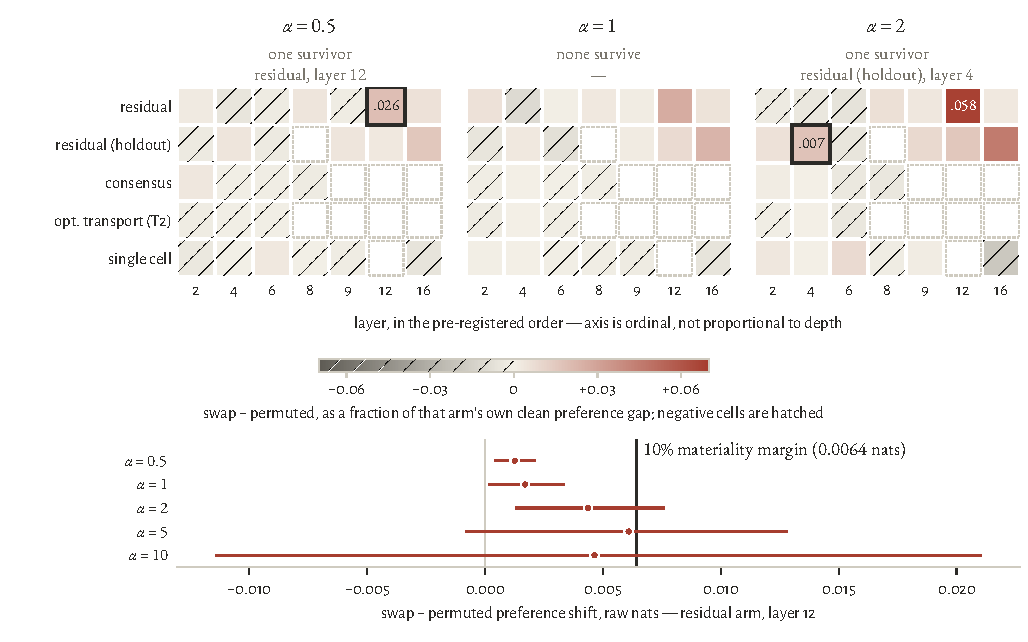
\includegraphics{family}
\caption[The single survivor moves with the rung]{\captiontitle{The one test that
survives multiplicity correction changes arm and depth with the rung of the
displacement ladder, and at one rung there is no survivor at all.} Each panel is
one slice of the ladder: the five training arms of \cref{tab:trainconfig} (rows)
by the seven probed depths (columns), $n = 26$ measured tests per slice, on one
diverging scale shared across the three panels. Colour is the \texttt{swap}
minus \texttt{permuted} effect as a fraction of that arm's own clean preference
gap. The layer axis is ordinal, drawn at equal spacing, and is not proportional
to depth. Nine of the $35$ grid positions were never measured and are drawn as
empty dotted outlines, not as zeros. Benjamini--Hochberg is pooled across arms
within a slice, as the text applies it and not as the pipeline stores it; $q$ is
printed in the three cells that fall below $0.10$ and ringed where $q < 0.05$.
That criterion admits the residual arm at layer $12$ at $\alpha = 0.5$
($q = 0.026$, on the stored bootstrap draw the text discusses), nothing at
$\alpha = 1$, and \texttt{residual\_holdout} at layer $4$ at $\alpha = 2$, which
demotes layer $12$ to $q = 0.058$; it is the only survivor among this chapter's
twenty-six headline tests. Beneath, the same residual arm at layer $12$ in raw
nats across all five rungs, with the $10\%$ pre-registered materiality margin as
the vertical rule. Intervals throughout are $95\%$ cluster bootstraps over
ordered (A,B) pairs, $4000$ resamples, which at this layer is $60$ rows in $58$
pair clusters over $24$ anchor drugs. }
\label{fig:family}
\end{fullwidth}
\end{figure}


% ===========================================================================
% NOTE TO SELF, removed from the printed title 2026-09-10: (REMEMBER TO CITE MERT KAAN THESIS)
\beatsection{E}{4}{Denoising the target changes the target, not the decoder}{sec:res-epsilon}

\begin{question}[4]
If the defect is a decoder that barely consults the drug region whatever is
written there, then improving what sits in that region should not help, and
improving the training target is exactly that kind of intervention. Three
target constructions, one scoring, one stratum. None separates from a prompt
naming the wrong drug.
\end{question}

\noindent
If the defect
is a decoder that barely consults the drug region whatever is written there, the
repair a reader reaches for first is to write something better there: give the
model a training target that carries the drug more legibly, and the region may
start earning the attention it currently does not get. That is a target-side
intervention, and it is the cheapest one available. The inference runs one way
only. A positive here would tell against the low-gain reading; a negative is
evidence about target-side fixes, not confirmation of the mechanism. Because one
failed construction proves nothing, two more were built and compared with it.

\paragraph{The original target, and what it starves} The single-cell arm trains
on a measurement and nothing else. A prompt names one control cell together with
the drug, its dose and its mechanism annotation; the response is the cell
sentence of a real treated cell drawn from that same condition. Nothing is
averaged, imputed or reconstructed, so the target is exactly something that was
observed. That is also the hypothesised defect. A single treated cell's rank
order is dominated by the same abundant genes whichever drug was applied, and the
drug displaces that cell by less than sampling noise does, so under next-token
cross-entropy the genes that distinguish one drug from another contribute almost
nothing to the gradient. On this reading the drug is not absent from the target;
it is present and outweighed.

\paragraph{Consensus, because aggregation is where the data separates drugs at
all} The motivation is measured rather than assumed. \Cref{sec:res-metrics}'s
spike-in forced choice separates two real drug populations essentially perfectly
once their cells are aggregated into a pseudobulk ($\paneltau = 1.000$,
$\DEdr = 0.995$, top-$n$ $\tau = 0.987$, plate held constant), and the within-well
precision reference climbs monotonically with the number of cells standing behind
a condition, $0.61$ at ten cells, $0.76$ at forty, $0.85$ at $120$
(\cref{fig:difficulty}, panel a). Whatever in this data distinguishes one drug
from another is a property of the averaged profile, not of any individual cell.
Consensus writes that average into the target directly. Cells are grouped by
(drug, cell line, dose), dose kept separate because most drugs are run at several,
each group averaged into a single pseudobulk profile, its genes ranked by mean
expression, truncated to the group's median cell length and closed with
\texttt{[END\_CELL]}. Every original prompt is retained and only the response is
swapped, so the example count is preserved exactly and the target is the sole
variable. The cost is structural: the map from prompt to target becomes
many-to-one, every control cell in a condition receiving the identical sentence,
so the heterogeneity is discarded along with the noise and there is nothing
per-cell left to learn. That objection is what the third construction answers.

\paragraph{Optimal transport, the middle the first two leave empty} The
measurement destroys the pairing it would be most useful to have. A condition
yields a cloud of control cells and a cloud of treated cells, and no cell appears
in both, so which control cell became which treated cell is not observed and
cannot be looked up. Optimal transport supplies the cheapest pairing consistent
with both clouds under an explicit cost, which gives a target that is denoised
like consensus and control-specific like the single-cell arm.

Conditions are keyed on the full tuple carried by the source, (cell line, plate,
drug, dose/treatment well), and each is solved separately, its treated cells
coupled only to the shared DMSO controls from that condition's own (cell line,
plate). Treatment conditions are never pooled, so batch identity cannot drive a
coupling. The coupling $\pi$ minimises $\sum_{ij}\pi_{ij}\lVert x_i - y_j\rVert^2$
under balanced uniform marginals, which impose mass conservation between the
empirical control and treated measures --- a modelling assumption, not an observed
biological constraint. Sinkhorn iteration~\cite{cuturi} solves it by alternately
rescaling rows and columns of the kernel $\Gamma = \exp(-C/\varepsilon)$, $250$
iterations, with $C$ the pairwise squared-distance matrix. The coupling becomes a
prediction through the barycentric projection
$T(x_i) = \sum_j \pi_{ij} y_j \big/ \sum_j \pi_{ij}$, a soft transport map
answering where \emph{this} control cell lands after treatment.

\paragraph{Where the coupling lives, and why the decoder is never called}
Optimal transport's sample complexity degrades badly in high dimensions, so the
coupling is not computed on raw expression. It is computed in the released Tahoe
scVI latent~\cite{scvi} ($n_{\textrm{latent}} = 10$). scVI is a variational
autoencoder for single-cell counts: an encoder maps a cell's counts to a
low-dimensional coordinate meant to capture its state, and a decoder maps such a
coordinate back to a distribution over gene counts. Tahoe's authors trained one
on the full corpus and distribute its output with the data --- the minified
\texttt{AnnData} object carries, in \texttt{obsm['X\_latent\_qzm']}, the posterior
mean of the latent for each of its $95.6$ million cells. The encoder has therefore
already been run once, by them, over every cell this work uses, and its result is
a stored per-cell $10$-vector rather than something to be recomputed. No scVI
model is instantiated anywhere in this pipeline. Each cell in the cache carries a
\texttt{BARCODE\_SUB\_LIB\_ID}, which is also the key indexing the shipped object's
rows, so attaching the latent is a lookup on that key: the $95.6$-million-row index
is streamed in chunks, the rows whose barcode appears in the cache are retained,
and their stored vectors are copied into cache order. All $620{,}564$ cells were
found.

The alternative --- running scVI locally over our own cells --- was tried first, and
it is worth recording because it failed without raising anything. Re-encoding
produced a latent in which a linear probe recovered the cell line at $0.11$
against $0.975$ for the shipped one: a latent that had lost the single strongest
structure in the data while remaining a perfectly well-formed array of the
expected shape. The cause is a schema trap rather than a modelling one. Tahoe's
per-cell \texttt{genes} field holds identifiers into the model's gene vocabulary,
not positional indices into the gene metadata table, and its values run past that
table's $62{,}710$ rows, so reading them positionally permutes gene identities
across the entire matrix. Nothing about the resulting expression looks wrong ---
the sparsity, the library sizes and the value distribution all survive --- and every
downstream quantity would have been computed on scrambled genes.

The mapping is therefore made explicit rather than assumed, and then tested. An
array indexed by vocabulary identifier is assembled from the gene metadata's own
\texttt{token\_id} and \texttt{gene\_symbol} columns and composed with the symbol
list of the $946$-gene L1000 panel the targets are built in; all $946$ panel genes
resolve. The test is the same probe that exposed the failure, run this time on the
panel rather than on a latent: principal components are fitted to $\log(1+x)$ of
the panel expression, $50$ components estimated on a random subsample of $60{,}000$
cells and used to project the remainder, and a multinomial logistic regression on
those coordinates is asked to name the cell line, three-fold cross-validated across
the $50$ lines holding at least ten cells. It reaches $0.864$ against a chance rate
of $0.02$. Permuted gene identities could not support that, so the panel is
correctly un-scrambled. The same components double as the coupling space held in
reserve, computed in parallel with the scVI latent so that the choice of embedding
is a setting rather than an assumption.

The latent's role ends with the cost matrix. It supplies the geometry in which one
control cell is judged near or far from one treated cell, and once $\pi$ has been
solved it is not used again: the coupling weights are applied to the condition's
observed treated expression vectors in the $946$-gene panel, library-normalised to
CP10K. The alternative would have been to average latent coordinates and map the
average back to counts, which is the one operation that would have required the
decoder, and it is declined on the grounds that a generative model fitted with no
knowledge of the drug is a poor thing to pass a subtle drug effect through --- it
would return whatever it holds a cell of that state to look like, which is a
prediction about the target rather than a measurement of it. Applying the weights
to observed cells instead makes every target a convex combination of real measured
cells: it lies inside the convex hull of that condition's treated cloud, though not
necessarily on the data manifold. Each is ranked descending and truncated to the
top $K$, where $K$ is the median number of expressed panel genes among that
condition's treated cells, and closed with \texttt{[END\_CELL]}; the prompt is the
same control cell in the same trainer format, so the examples are drop-in
compatible with the other arms. Applied at $\varepsilon = 0.5$ to the $3{,}856$
conditions holding at least sixty treated and sixty control cells, this yields
$381{,}485$ training examples. Two properties were checked before any training ran:
the targets vary across control cells within a condition, which is the property
consensus lacks, and they reproduce the treated cloud they were built from, their
pseudobulk sitting $0.006$ from the real treated pseudobulk.

\paragraph{Three points on one knob, not a sweep} Set out this way the three
constructions turn out not to be three ideas but one, at three settings. The
regularisation parameter of the middle arm interpolates between the other two: as
$\varepsilon\rightarrow\infty$ the coupling becomes uniform, every control cell is
matched equally to every treated cell, and the barycentric target collapses to the
treated mean, which is consensus; as $\varepsilon\rightarrow 0$ the coupling
sharpens towards an unregularised sparse transport solution, close to handing each
control cell one state-matched treated cell, which is the single-cell regime,
though the limit is not literally a map onto an observed cell. That the family
lines up this way was not the order in which it was built --- the single-cell target
came first because it is what the corpus supplies, consensus second for the
aggregation reason above, and optimal transport last, to occupy the middle they
leave empty --- but it is how the three should be read.

The reading buys something and it is worth being exact about how much. Three
unrelated failed constructions would be three anecdotes, and a fourth could always
be proposed; endpoints and midpoint of a single one-parameter family are harder to
dismiss as an unlucky choice of target, because the thing being varied is the one
quantity that distinguishes them. What it does not buy is coverage. Three
hand-picked settings were trained and scored, so nothing here is a sweep: no
intermediate $\varepsilon$ was run, the three points cannot interpolate the
interior, and a construction outside this family --- a target built on a different
cost, a different embedding, or no transport at all --- is untouched by the result
either way.

\paragraph{One scoring, named before the result} The three arms differ in their
training target and in almost nothing else about how they were trained: each is
cold-started from the same base checkpoint under the identical hyperparameter set
(\cref{tab:trainconfig}), and each is scored on the same held-out-drug conditions
through one instrument fixed before any arm was read. The exception is length.
Single cell and optimal transport each complete their epoch; consensus was
scheduled for one and stopped by the wall-clock at $61.5\%$ of it
(\cref{fig:training}), so its null carries an under-training confound the other
two do not. Holding the evaluation
fixed is what leaves the target as the variable of interest, so it is worth being
explicit that none of the three is scored on its own target. All are scored against a pseudobulk of real treated cells from the drug's own well — a tier-2 condition throughout, as in \cref{sec:res-blind} — split in two: one half the scoring truth, the other the within-well split-half precision reference

What the two new targets were supposed to buy follows from where the drug signal
lives. \Cref{sec:res-metrics} found it emerges only under aggregation: at
single-cell resolution two drugs are indistinguishable, and it is the pseudobulk
that separates them. The single-cell arm is trained on individual treated cells
and then graded on aggregates, so it is asked to learn in the resolution where
the drug is invisible and perform in the one where it is not. Consensus and
optimal transport close that gap from the training side --- a group mean and a
state-matched barycentric combination respectively, both aggregates, both in the
space the evaluation reads. If drug-specific structure only becomes legible after
averaging, a target that is already averaged should be the one that teaches it.

That every arm is graded against the same object — a pseudobulk of half the condition's real treated cells — rather than against the aggregate each was trained to emit looks like it should penalise exactly those two, and at the resolution this instrument works in, it does not. Write $Y$ for a condition's $n_t$ treated cells and $\pi$ for
the entropic coupling described above, whose uniform marginals give
$\sum_j \pi_{ij} = 1/n_c$ and $\sum_i \pi_{ij} = 1/n_t$. The optimal-transport
target for control cell $i$ is $\hat{y}_i = (\pi Y)_i \big/ \sum_j \pi_{ij}$, and
averaging it over the condition's control cells gives
\begin{equation}
 \frac{1}{n_c}\sum_{i} \hat{y}_i
 \;=\; \sum_{i}\sum_{j} \pi_{ij}\, y_j
 \;=\; \sum_{j} y_j \sum_{i} \pi_{ij}
 \;=\; \frac{1}{n_t}\sum_{j} y_j ,
\end{equation}
the condition's treated mean exactly. The consensus target is a group mean of
treated cells by construction, and the truth used here is a half-split estimate
of the same quantity. At pseudobulk resolution the three native targets and the
scoring truth are one object, so scoring every arm on real cells is not a
compromise imposed on two of them --- it is their own target, read at the
resolution the metric works in. What the scoring discards is each arm's
\emph{per-cell} specificity, not the identity of its target.

The instrument is read twice, and the two readings ask different questions. The
first asks whether naming a different drug changes the prediction at all: one
number per arm, with the substituted drug drawn at random, taken on the
identifiable stratum of \cref{sec:res-blind} --- the $\num{204}$ of $\num{606}$
held-out-drug conditions whose own within-well reference clears the pre-set
$0.80$ bar, where the ranking is known to be winnable. The gap is
\ci{+0.014}{-0.016}{+0.042} for single cell, \ci{-0.001}{-0.018}{+0.016} for
optimal transport and \ci{-0.010}{-0.022}{+0.003} for consensus; none separates.

A randomly drawn partner, though, sits at an arbitrary distance from the real
drugm sometimes a near-twin whose response is almost the right answer anyway,
sometimes an opposite. Each of those three numbers averages over that whole
range, and the near-twins pull it toward zero, so an arm that responded to the
drug only when the substitute was very unlike it would still read null.

The second reading separates those cases instead of averaging them. Every partner
was recorded when the scramble was built, so each condition carries a measured
distance between its own truth and its partner's, and its gap can be read against
that distance rather than pooled across it; an arm that uses the drug should show
a gap that grows with it. Binning by distance needs more conditions than a single
number does, so this reading runs over all $\num{454}$ tier-2 conditions whose
substituted partner also has a truth profile, not the $\num{204}$ identifiable
ones. \Cref{fig:sweep-arms} draws the two new constructions only: the single-cell
arm's sweep was run directly, with partners chosen to span the distance range
rather than reconstructed from random draws, and is \cref{fig:sweepbins}.

One limit travels with every number here. The identifiable stratum is exactly
where a zero-drug-information control-copy already matches the model, so the
scope limit of \cref{sec:methods-probe} applies throughout: a null is a null
about drug use, not a statement that the arms predict nothing.

% ===========================================================================
% ---------------------------------------------------------------------------
% ---------------------------------------------------------------------------
% ---------------------------------------------------------------------------
% ---------------------------------------------------------------------------
\begin{figure}[htbp]
\begin{fullwidth}
  \raggedright
  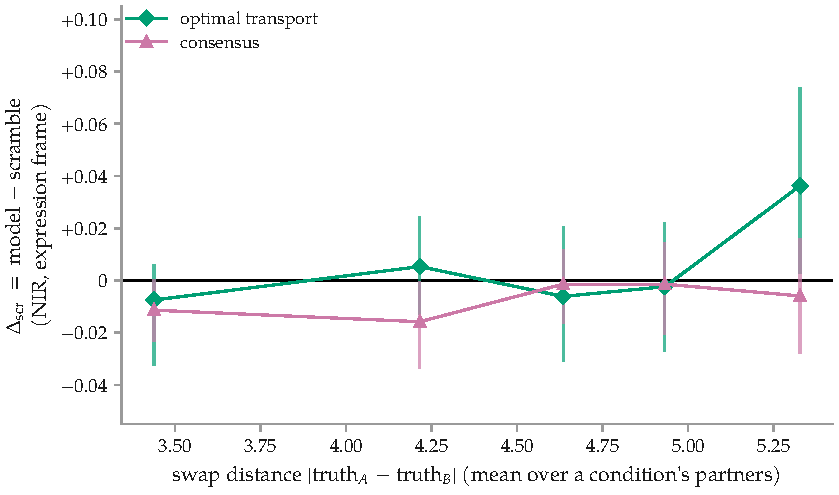
\includegraphics{fig-sweep-arms}
  \caption[Neither new target orders its gap by swap distance]{\captiontitle{Optimal
  transport separates from its scramble only at the most dissimilar partners, and
  consensus not at all; neither produces the ordering across the range that drug
  sensitivity would give.} Each point is a quintile of conditions binned on swap
  distance, the Euclidean distance $\lVert\textrm{truth}_A -
  \textrm{truth}_B\rVert$ between the real drug's half-A pseudobulk and the
  substituted drug's, computed within one (cell line, plate) group so the control
  cancels --- the same distance \cref{fig:sweepbins} uses, over a comparable range.
  The single-cell arm is not drawn: its sweep was run directly, with partners
  chosen to span the distance quantiles rather than reconstructed from random
  draws, and is reported in \cref{fig:sweepbins}. An ordered effect would climb
  across all five bins. Consensus is flat and negative throughout, never crossing
  zero. Optimal transport changes sign twice across the first four bins and then
  reaches \ci{+0.036}{+0.003}{+0.074} in the farthest --- one of two intervals
  among the ten drawn here that exclude zero, and the only one to do so from
  above; the other is consensus's second bin, \ci{-0.016}{-0.034}{-0.0005}. The per-condition correlation between
  distance and gap, which no choice of binning affects, is $+0.074$ for optimal
  transport and $+0.045$ for consensus. The scramble partner was drawn
  independently \emph{per cell}, a median of six distinct partners per condition,
  so each condition's score already averages over a mixture of distances and is
  placed at its mean partner distance; the design cannot isolate a single sharpest
  partner the way \cref{sec:res-encoding}'s ladder does. $n = \num{454}$ of the
  $\num{606}$ tier-2 conditions, those whose substituted partner also has a truth
  profile in the same group; intervals are $95\%$ cell-line-clustered bootstraps,
  $\num{2000}$ resamples.}
  \label{fig:sweep-arms}
\end{fullwidth}
\end{figure}
% ===========================================================================
% ---------------------------------------------------------------------------
\paragraph{Optimal transport reaches the far end and nothing before it} Read
against how dissimilar the substituted drug was, the two aggregated targets do
not behave identically, and the difference is worth stating precisely rather than
collapsing into a shared null. Consensus is flat and negative at every distance,
drifting from $-0.011$ to $-0.006$ without once crossing zero: on this evidence
it never distinguishes the drug it was named from any other, however unlike them
it is --- though it is also the arm that stopped short of its epoch, so its flat
line is the one reading here with two explanations rather than one. Optimal transport does something, but only at one end. It changes sign twice
across the first four bins and then reaches
\ci{+0.036}{+0.003}{+0.074} against the most dissimilar partners --- so when the
substituted drug's true response is as far from the real one as this atlas
allows, the model's output does register the difference.

That is a real if narrow finding, and it is also not what drug sensitivity looks
like. A model reading the drug should separate a little from a near-twin and more
from an opposite, with the gap growing across the range; what optimal transport
gives is nothing across four bins and a single excursion in the fifth. The
per-condition correlation, which no choice of binning affects, is $+0.074$ ---
indistinguishable from no relationship. One endpoint clearing zero out of ten
unadjusted intervals is the weakest form the evidence could take while still
being non-zero.

The same regression settles the ordering question for this arm directly. A
purpose-built sweep exists for it, with partners chosen to span the distance
quantiles rather than drawn at random, five per condition --- which is what the
reading of \cref{sec:res-blind} needs. For condition $i$ and its $k$th scrambled
prompt, regress that prompt's $\NIR$ on the negated Euclidean distance between the
condition's own truth and the truth of the drug substituted into it,
\begin{equation}
 y_{ik} \;=\; \alpha_i \;+\; \beta\,x_{ik} \;+\; \varepsilon_{ik},
 \qquad k = 1,\dots,5,
\end{equation}
with one intercept per condition, the target-drug prompt excluded so that no
comparator enters, and $x$ negated so that it rises with similarity. A model that
never reads the name puts its five points at one height, so $\beta = 0$ is the null
by construction and $\beta > 0$ is what sensitivity would look like.

The arm returns the null. Pooled across conditions the slope is $+0.0485$
$[-0.0287, +0.1256]$ clustered on drug, already covering zero; fitted within
condition it is $-0.0008$, $[-0.0305, +0.0290]$ clustered on drug and
$[-0.0247, +0.0232]$ on cell line, over $200$ prompts across $40$ conditions.
Almost all of the pooled figure was the between-condition comparison that the
intercepts remove, $+0.0790$ of it. The within-condition interval is narrow enough
to exclude any effect a tenth the size of the pooled one, so this is a measured
null and not an absence of power: whatever aggregating the target bought, it was
not sensitivity to the drug the prompt names. One scope limit travels with it.
The sweep was scored at $1200$ tokens, and the separate reading that this arm is
inert has been withdrawn on exactly that ground.
What the regression establishes survives that withdrawal, because it is narrower:
no graded response to how unlike the substituted drug is.

That leaves a genuine question about what the training did accomplish, since it
was plainly not inert. The consensus model stops echoing the control: on the
identifiable stratum it scores $0.653$ against a zero-drug-information
control-copy at $0.766$, where the single-cell model sits on the control at
$0.768$. Its predictions are not mode-collapsed either; there is real
between-condition variation. But that variation is uncorrelated with real drug
identity --- the Mantel correlation between the model's between-drug distance
structure and the true one averages $+0.03$ over cell-line and plate groups. The
failure this literature names first for a perturbation model that underperforms
on well-calibrated metrics is mode collapse, where the prediction ignores the
input and reverts to a mean, and the repair is to restore diversity in what the
model emits~\cite{mejia}. This arm is not that. It moved off the control, kept
the variation, and spent it on the wrong axis. Producing no structure and
producing structure that does not track the drug are different failures with
different repairs.
% ...........................................................................
% 04c-reencoding.tex -- beats 5-6. The residual re-encoding.
% Legacy anchors sec:methods-vardecomp and sec:methods-holdout are re-\label-ed
% here so v1 cross-references resolve.
% ...........................................................................

\beatsection{R}{5}{The standard target hides the drug}{sec:methods-residual}

\begin{question}[5]
  Every target compared in the last section ranks genes by how much of them a cell
  holds, and two drugs on the same cells hold almost the same genes in almost the
  same order, so the loss can barely tell those targets apart. The apparatus chapter
  defines a target that ranks something else instead. Does it in fact expose the
  drug, and can it be estimated without the evaluation leaking into the fit? The
  instrument counts how many top target positions carry a different gene for two
  drugs in one context. 
  \end{question}

  \noindent
  \Cref{sec:res-epsilon} ended on a distinction it did not resolve: producing no
  structure and producing structure that does not track the drug are different
  failures. This section takes up the second, and it opens by conceding the first.
  Three target constructions were tried there and none separated, so a fourth
  arrives owing an explanation of why it is not simply a fourth point on the same
  ladder.
  
  It is not, because that ladder held one thing fixed. Every target in
  \cref{tab:epsilon} ranks genes by how much of them the cell holds and varies only
  how many cells are averaged before the ranking is taken. Averaging changes how
  noisy a ranking is; it does not change what the ranking is \emph{of}. Two drugs
  applied to the same cells leave the same abundant genes at the top in nearly the
  same order, so every point on that ladder inherits nearly the same target string
  however cleanly it is estimated --- which is what \cref{sec:res-epsilon} meant in
  reserving judgement on constructions outside its family.
  \Cref{sec:apparatus-vocab} defines one. What follows is the measurement that
  motivated it and the analysis of whether it can be estimated at all.
  
  \emph{Encoding} here means how the target string is written, not what the model's
  internal states carry (\cref{sec:res-used}). The loss weights every position
  equally, so the measurement is a count over the $200$ target positions
  (\cref{tab:divergence}).
  
  % ...........................................................................
% ...........................................................................
\begin{table}[htbp]
  % MARGINALIA: full width; the long caption sets above at the text width,
  % notes below in the sans. One rule, under the head.
  \caption{\captiontitle{$83\%$ of the standard target's tokens are identical between any
  two drugs in the same context; under the residual, $40\%$ are --- and the
  residual's exposure does not track how similar the two drugs' responses are.}
  Rows are quoted at the plate scope this build uses (\cref{sec:apparatus-vocab});
  at cell-line scope the residual row reads $118.2$ overall and $0.7432$, and the
  other two rows are unchanged. The three stratum columns bin all $\num{212528}$
  exhaustive within-group drug pairs on the cosine between the two residuals ---
  near above $+0.1$ ($n = \num{23024}$), orthogonal within $\pm 0.1$
  ($n = \num{152421}$), opposite below $-0.1$ ($n = \num{37083}$) --- on the same
  similarity axis and the same cut points the later swap evaluation uses. The full
  profile and the shift climb monotonically across those strata and correlate
  negatively with residual cosine; the residual stays high in all three and does
  neither. That weakens the reading that the later swap-distance pattern is
  inherited trivially from target divergence rather than being an independent test
  of it. The counts are where the three encodings differ, and they do not on their
  own identify tokenisation as the binding constraint.}
  \label{tab:divergence}
  \begin{fullwidth}
  \begin{threeparttable}
  \begin{tabular}{@{}l r@{\hspace{0.4em}}l r r r r r@{}}
  & \multicolumn{5}{l}{\thead{Top-$200$ tokens differing between drugs}}
  & & \\
  \addlinespace[2pt]
  \thead{Representation} & \thead{all pairs} & & \thead{near} & \thead{orth.}
    & \thead{opposite} & \thead{$\rho$}
    & \thead{Retrieval reference} \\
  \midrule
  full profile (the standard target)
    & $34.6$ & ($17\%$)  & $32.5$ & $34.6$ & $35.8$ & $-0.149$ & $0.742$ \\
  shift (treated $-$ control)
    & $111.4$ & ($56\%$) & $107.4$ & $111.3$ & $114.5$ & $-0.282$ & $0.742$ \\
  residual (shift $-$ generic)
    & $120.3$ & ($60\%$) & $118.4$ & $121.0$ & $118.7$ & \key{$+0.019$} & $0.7467$ \\
  \end{tabular}
  \begin{tablenotes}[flushleft]
  \item The count columns and the retrieval column hold different quantities, a
  tally out of $200$ positions and a retrieval score, so rows compare within a
  column and never columns with each other. $\rho$ is the Spearman correlation
  between a pair's residual cosine and its differing-token count, taken over all
  pairs and not within a stratum.
  \item The retrieval column pits disjoint cell subsets of one drug, in one cell
  line, on one plate, against each other. It is a precision reference, not a
  biological replicate ceiling, and it is near-constant across the three rows: the
  rewrite exposes the drug without buying that exposure from a coarser measurement.
  \item The stratification is descriptive. Pairs reuse drugs and experimental
  groups, so no pair-level inferential claim is made and no interval is drawn.
  \end{tablenotes}
  \end{threeparttable}
  \end{fullwidth}
  \end{table}
  \paragraph{Which subtraction does the work} Removing the control moves the
  between-drug token difference from $34.6$ to $111.4$; removing the generic adds a
  further $8.9$ at the plate scope this build uses, and $6.8$ at cell-line scope. So
  the control subtraction alone buys $90\%$ of the recoverable difference, $92\%$
  cell-line-scoped. That is the first thing the table says and the least comfortable
  one for the construction it motivates: almost all of the exposure comes from the
  cheaper of the two subtractions. The measurement is an overlap of gene sets on one
  atlas at $K = 200$ ($\num{6602}$ conditions, \texttt{target\_divergence.json}), so
  no margin is claimed for other atlases or other $K$. It squares with
  \cref{sec:res-metrics}, where what saturates $\DEdr$ is reversion toward a central
  point, \texttt{revert\_center} scoring $0.9999$ without fitting anything.
  
  Read as a verdict on the generic, though, that $90\%$ proves less than it looks
  like, and the reason is in what the count counts. It tallies how many of the $200$
  positions carry a different gene between two drugs, so a subtraction is credited
  only where it reorders the two drugs' rankings differently \emph{from each other}.
  Removing a component the two drugs share does that weakly by construction, however
  large the component is. As we show further in later sections however, by magnitude the split runs the other way: the shift's
  squared norm decomposes into a drug-specific residual of $0.621$, a generic
  programme of $0.390$ and a cross term of $-0.011$. The generic is two fifths of
  what the control subtraction leaves behind, and it is very nearly orthogonal to
  the part that identifies the drug.
  
  Thus the two subtractions are not competing for one credit, then. The control
  subtraction is what exposes positions to the drug at all, and the generic
  subtraction decides what those exposed positions are about --- a target that
  skipped it would rank each drug's genes against a baseline still carrying two
  fifths of the programme every drug triggers. Neither is dispensable, and
  \cref{tab:divergence} is simply the wrong instrument for asking whether the second
  one is.
  
  One threshold choice belongs beside these counts. The inclusion minima of
  \cref{sec:apparatus-vocab}, at least $40$ treated and $20$ plate-matched control
  cells, sit where the identifiability curve of \cref{sec:res-blind} flattens: the
  within-well split-half precision reference reads $0.61$ at $10$ cells, $0.76$ at
  $40$ and $0.85$ at $120$.
  
  \paragraph{The count stops short of the tokenisation claim} The natural inference,
  that only a small fraction of the gradient carries drug identity, is a hypothesis
  about the optimisation; what is measured is the overlap of target gene sets, not a
  token-level loss or a gradient attribution. Gene positions are not loss-token
  positions under byte-pair encoding, and the residual target alters aggregation,
  control referencing, generic subtraction, sign coding and sequence length at once.
  Separating those five factors needs a matched-budget factorial this thesis does not
  run.
  
  
  % ...........................................................................
  \paragraph{What the plate-local generic costs, measured}
  \Cref{sec:apparatus-vocab} states the limit as part of the definition: what
  survives both subtractions is not what makes this drug different from all drugs,
  but what makes it different from the other training drugs sharing its plate and
  cell line. Stated there it is a definitional caveat. Here it is a quantity, and
  mechanism is where it bites. \Cref{sec:res-scope} finds mechanism-related drugs
  co-plated $0.404$ of the time against $0.362$ for a random draw, so for a co-plated
  mechanism class part of the class's own shared programme sits inside the generic
  and is subtracted out of every member's residual by construction.
  
  That bias was tested rather than assumed, and the mechanism gate of
  \cref{sec:res-scope} is where it can be, because that gate is scored in this
  frame.

  \begin{scopelimit}[carried into \cref{sec:res-scope} and \cref{sec:limitations}]
  Two properties of this frame travel with every number measured in it. First, the
  generic is a plate-local mean, so where a mechanism class is co-plated the
  mechanism channel is later graded in a frame that has already removed some of what
  it is asked to find, which makes an inconclusive verdict on mechanism the
  conservative reading and not a generous one. Second, the plate-scoped generic
  removes plate structure from the truths and, in expectation, from the predictions,
  but that is an expectation and not an identity. An individual residual may retain
  some plate structure, and the size of what remains was never measured. The absolute
  $\NIR$ values of this frame are read within it and never set beside the
  within-plate tables elsewhere in the chapter.
  \end{scopelimit}
  
  % ...........................................................................
\paragraph{Estimating the generic is where leakage would enter} The residual is a
subtraction, and the quantity subtracted is not handed down by the design: it is
estimated from the same data the model is trained and scored on. That makes the
generic the one part of the construction capable of going wrong in a way the
target string never shows. This is particularly concerning if we wish to perform preprocessing on conditions and admit only conditions that carry signal and not noise. A leaky generic still produces well-formed sentences of
plausible genes; it simply produces them against a baseline that has already seen
what the model is about to be tested on. \Cref{sec:apparatus-vocab} states two
properties of $D_c$ as fundamental, leave-one-drug-out and split-before-fit,
without arguing for either. They are argued here, because between them they settle
the two questions an estimated subtrahend raises: what the mean is taken over, and
which conditions are allowed into it.

\paragraph{The mean is over drugs, and a condition's own drug leaves it entirely}
The generic is built in two steps rather than one. Within a group, each drug's
conditions are first averaged into a single per-drug shift; the generic is then the
mean of those per-drug shifts. Both steps carry weight. Averaging within a drug
first is what makes the result a mean over drugs at all: otherwise a drug measured
at five doses in the group would contribute five terms and count five times as
heavily as a single-dose drug, and the generic would be a mean over conditions
wearing the name of a mean over drugs.

\emph{Leave-one-out} then names a removal that could be drawn at several levels,
and the level is what the rule is about. What is removed is the drug. When the
generic for a condition is formed, that condition's drug is struck from the group's
roster altogether --- every dose of it and every condition of it, not merely the one
condition whose residual is being computed --- and the mean is taken over the drugs
that remain. The narrower alternative, dropping only the condition itself, sounds
equivalent and is not. A drug run at five doses would keep four of its own
conditions inside the mean subtracted from its fifth, so part of what that drug does
would be subtracted from itself, and the residual would answer a different question:
what makes this dose unlike this drug's other doses, rather than what makes this
drug unlike the other drugs. Removing at drug level is what guarantees that the
quantity subtracted from a condition carries no information about that condition's
drug.

The rule also keeps the two splits commensurable, which is the reason less often
noticed. The generic is fitted on training conditions only, so a training
condition's drug sits in the fit inventory and, without the rule, would appear in
the mean subtracted from itself. A held-out condition's drug contributes nothing to
its group's generic in any case, because the split holds out every condition of that
(drug, cell line) pair. The two splits would therefore be scored against
differently defined targets, and a comparison between them would be confounded by
the definition rather than by generalisation. Leave-one-drug-out removes the
asymmetry by making both sides alike: neither has its own drug in its own generic.

\paragraph{Which conditions may enter the generic, and what makes the question
hard} The second question has an answer that raises no difficulty whatever: every
condition the split assigns to training. Fitting the generic on that set is one
pass over fixed data, nothing in it refers to any quantity computed later, and
there is no circularity to speak of. The difficulty is introduced deliberately,
by us, and it is introduced for a reason worth keeping.

Not every condition carries a residual worth training on. At this cell budget the
two subtractions can leave a vector that is almost entirely sampling noise, and
such a condition still emits a full-length target string --- ranked, closed with
\ENDCELL{}, indistinguishable in form from any other --- which the loss weights
exactly as heavily as a condition whose residual is real. Training on it teaches
the model to reproduce noise in the voice of a drug effect. The scale of that is
not marginal: the line finally adopted retains half the training conditions, which
is another way of saying that the median condition's two halves agree about as
well as two unrelated conditions' halves do. A filter is worth having, and the
natural test for one is self-consistency.

That test is the half-split, and its content is precise. A \emph{condition} ---
one drug, at one dose, on one cell line, on one plate, the unit of
\cref{sec:methods-data} --- has its treated cells shuffled and cut in two, and the
plate's control cells are cut in two alongside them; the same halving is applied
to every other condition in the same (cell line, plate) group. Each half yields a
shift, its treated mean minus its control mean, computed inside that half alone.
Each half also yields a generic, the leave-one-drug-out mean just described taken
over the other training drugs' shifts on the matching half. Subtracting the one
from the other leaves two residuals that share no cell and no estimate, and the
condition is kept only if the cosine between them clears a threshold. Two
independent measurements of the same condition must agree before it is allowed to
teach anything.

Adding that test is what closes the loop. It decides membership of the training
set, and it decides it from the residual --- which is a shift minus the generic,
and the generic is a mean over the other \emph{training} drugs. Membership is
therefore settled by a quantity that is itself a function of membership. Note
where the problem is not: nothing in the test is recursive, since a shift needs
only cell means and a generic needs only other drugs' shifts, so for any fixed
list of training drugs every quantity computes in a single pass and a condition's
residual never requires its own residual. The circularity sits one level up and it
is about \emph{membership} alone. Written as edges: the reliability line selects
the training set, the training set fits the generic, the generic is subtracted to
give the residual, and the residual is what the reliability line is applied to
(\cref{fig:circularity}, left). Every edge is defensible on its own, the four
close, and nothing in the definitions says where to start.

What that would cost is not abstract. Suppose the generic were refitted on the
conditions the filter retains, which is the natural reading of ``the mean over the
drugs we are actually training on''. Dropping one condition would then change the
generic of every other condition in its group, hence their residuals, hence which
of \emph{them} pass --- so whether a condition survived would depend on when it
was evaluated, and the procedure would have to be iterated to a fixed point that
nothing guarantees to exist or to be unique.

So the design problem is not whether to filter but where to let the filter act. It
must be allowed to decide what the model trains on, which is the whole point of
it, and it must not be allowed to decide what the generic is fitted on, which is
what would close the circle. Those two can be separated, because they are separate
sets: the fit inventory is fixed by the metadata split, and the filter operates
downstream of it on conditions whose residuals have already been computed. The
generic is fitted once, on every condition the split assigns to training, before a
single reliability test has run; the filter is one terminal pass against that
fixed estimate; and dropping a condition moves no other condition's residual. The
retained set is a function of the data and not of the order it was walked in.

The hazard is set out at this length because an earlier build of ours was in it,
estimating generic and filter over every condition and assigning the holdout
afterwards. That adds a fifth edge to the figure, held-out conditions entering the
fit, and makes each held-out target partly a function of the other held-out
conditions. The failure is quiet: it survives every check that inspects the
targets themselves, since the targets it produces look exactly like the ones it
should have produced. Any construction that estimates what it subtracts, and then
filters on what is left, is exposed to some version of it.

\paragraph{The loop is cut by ordering, and the ordering is enforced} The build runs
as \emph{inventory}, \emph{split}, \emph{fit}, \emph{transform}, and each stage may
read only what the stage before it is allowed to expose (\cref{fig:circularity},
right). Inventory enumerates conditions from metadata and cell counts alone --- the
(drug, cell line, plate, dose) tuples clearing $40$ treated and $20$ plate-matched
control cells --- and aggregates no expression at all. Split then assigns train and
holdout from that metadata, keyed on the (drug, cell line) pair so that every dose
and every plate of a held-out pair leaves with it, and it does so before a single
pseudobulk exists. That removes the first edge: nothing downstream can have defined
the split, because at the moment the split is written there is nothing downstream to
define it with.

Fit estimates the generic, and is handed the training keys explicitly rather than
inferring them. Its inventory is every condition the split assigned to training,
taken whole and before any reliability test has run, which removes the second edge
--- admission cannot select the fit inventory, because the fit inventory is fixed
before admission is decided. Within that inventory the estimator is the one argued
above, drug-weighted and leave-one-drug-out, scoped to the (cell line, plate) group
and failing closed where a group holds fewer than three other training drugs, in
which case the condition is dropped and counted rather than quietly falling back to
a coarser scope. Transform then projects every condition, held-out ones included,
through that fitted generic. Held-out conditions are scored by it and never enter
it.

The training set is made last, and in a single pass. Each training condition's two
half-residuals are formed against the fixed generic, their cosine is taken, and the
condition is kept if it clears the line, $2{,}523$ of the $\num{4999}$ training
conditions or $50.5\%$. Because the generic is never refitted on the survivors, a
drop moves no other condition's residual and the retained set does not depend on the
order the pass walked in. Held-out conditions are transformed but deliberately not
filtered. Each retained condition then emits one training example per plate-matched
control cell, the prompt carrying that control cell together with the drug, its dose
and its mechanism annotation, and the response being that condition's residual
string.

The staging is checkable rather than merely asserted. A poison test corrupts every
held-out expression vector with large noise, rebuilds, and requires both the
training \texttt{JSONL} and a hash of every fitted quantity to be
unchanged.\gloss{poison test}{Corrupt the held-out side; the training targets and
the fit digest must not move. Corrupt a training condition; they must.} If one
held-out cell reaches the fit, one of the two moves, and restoring the earlier
build's one-line defect does make it fail on the digest, so the check is not
vacuous. Poisoning a training condition instead must change both, which is the
negative control that stops it passing for the wrong reason. One quantity the
staging does not settle is the threshold the filter applies, and that is the last
piece.

% ===========================================================================
% circularity.tex -- the residual definition's loop, and the ordering that cuts
% it. \input by Sections/04c-reencoding.tex at sec:methods-residual. Compiles
% against thesis_v2/preamble.tex and nothing else: no external data, no
% \includegraphics, no package this document does not already load
% (tikz + arrows.meta, both in preamble.tex section 9).
%
% THIS IS A PROVENANCE DIAGRAM, NOT A RESULT. Deliberately absent: every NIR
% value, every arm, every split-level number. Two counts appear, once, and both
% are already in the prose of this same section. Sibling circularity.json lists
% every number drawn.
%
% THE LEFT PANEL CARRIES NO BUILD LABEL, DELIBERATELY. It drew "THE EARLIER
% BUILD -- NOT THE SHIPPED ONE" until this revision, which spent half a
% full-width figure on a pipeline the thesis did not run. The historical fact
% -- that an earlier build did close this loop -- is a disclosure, and a
% disclosure belongs in prose where it can be qualified: it is stated at
% Sections/04c-reencoding.tex:148-151 ("That is a loop [...], and an earlier
% build closed it, with generic and filter estimated over every condition and
% the holdout assigned afterwards"). That sentence stands on its own and was
% NOT deleted when the label came off the panel. What the left panel draws now
% is the structural hazard itself, in the present tense and attached to no
% build: the cycle the four definitions form, and the edge that fitting before
% splitting adds to it. The two panels therefore read hazard and remedy, which
% is the only reason the staged ordering is load-bearing rather than fastidious.
%
%   2,523 of 4,999 training conditions retained (50.5%)   04c-reencoding.tex:211-212
%   the resolved reliability line, +0.1086                 04c-reencoding.tex:211
%
% Cross-checked, all four agreeing, before drawing:
%   Sections/03-Apparatus.tex:206     "2,523 of 4,999 train (50.5\%)"
%   Sections/04c-reencoding.tex:212   "$2{,}523$ of $\num{4999}$ ... ($50.5\%$)"
%   Sections/04d-baselines.tex:337    "only $\num{2523}$ are training"
%   Sections/05-Limitations.tex:33    "$\num{2523}$ of $\num{4999}$ ... $\cos > 0.109$"
% +0.109 is the measured null's 95th percentile and +0.1086 is what it resolves
% to; the prose prints both, and the node carries the resolved value because
% that is the one the builder applies.
%
% LAYOUT NOTES, all forced by a build:
%   * fullwidth = 174mm = 493.23pt (textwidth 142mm + marginparsep 4mm +
%     marginparwidth 28mm, preamble.tex:88-90 and :525). The bounding box is
%     PINNED to 17.35cm = 491.81pt, 1.4pt inside the measure. Unpinned, the
%     picture measured 3.10pt OVER and the figure body reported an overfull
%     hbox: nodes with anchor=north west hang their 3.33pt inner sep left of
%     the anchor at x=0.20, and the strip rules end at x=17.35. Pinning clips
%     no ink -- no drawn object lies outside [0, 17.35] x [-0.95, 7.95].
%   * NO node uses text width. Every line break is written by hand. The first
%     build did use text width and TeX hyphenated inside the boxes
%     ("the relia-/bility line"), grew four of them past their minimum heights
%     and overlapped the rows below. Hand-broken lines make every box width and
%     height deterministic, which is what lets the coordinates below be trusted.
%   * the four objects are ONE node set drawn twice, same style, same wording,
%     same 2.80cm minimum width, so the right panel reads as a re-laying of the
%     left and not as a second diagram. Only the arrangement changes.
%   * the fatal edge is drawn and STRUCK, not deleted. A deleted edge leaves
%     nothing for the caption to point at, and the passage is about which single
%     edge the ordering removes.
%   * the two streams leaving SPLIT must not cross. They cannot both turn upward
%     in the order they leave: the stream that leaves HIGHER (held-out, 2.2mm
%     above the east anchor) turns up FIRST (x=10.30) and the stream that leaves
%     LOWER (training keys, at the east anchor) turns up LATER (x=10.85). Any
%     other pairing crosses, and a crossing here reads as contact between them.
%   * both streams use -| rather than an explicit corner coordinate, so the
%     corner inherits the node anchor's own y. Written as a literal corner, the
%     first segment came out as a visible diagonal whenever a node's height
%     differed by a hair from the value assumed at design time.
%   * the held-out stream is routed over the top of the fit column, and its one
%     arrowhead points right, into TRANSFORM. No arrowhead anywhere in the right
%     panel points back left or up into the fit; that absence is the claim.
%   * NO edge label is masked onto its arrow. The first build masked all of
%     them and the labels ate the edges: the C->D gap in the left panel is
%     1.20cm and "subtracted to give" is 1.15cm wide, so the bottom edge of the
%     cycle disappeared and the loop stopped reading as a loop. Every label now
%     sits beside its edge. The tightest is "training keys", hung under the
%     corner at x = 10.43 to 11.27, between the held-out riser at 10.30 and the
%     fit column's left edge at 11.35.
% ===========================================================================
\begin{figure}[htbp]
\begin{fullwidth}
\centering
\begin{tikzpicture}[x=1cm, y=1cm]
  \useasboundingbox (0,-0.95) rectangle (17.35,7.95);
  \tikzset{
    % the shared node set. Identical style in both panels.
    obj/.style={draw=rulegrey, line width=0.4pt, fill=white, inner sep=3pt,
                align=center, font=\scriptsize, text=ink,
                minimum width=2.80cm, minimum height=0.68cm},
    edg/.style={-{Stealth[length=3.6pt,width=2.8pt]}, draw=ink,
                line width=0.5pt},
    lab/.style={font=\scriptsize, text=quietink, fill=white, inner sep=1pt,
                align=center},
    side/.style={font=\scriptsize, text=quietink, align=flush right,
                 anchor=east, text width=3.20cm},
    quiet/.style={font=\scriptsize\itshape, text=quietink, align=center},
    tag/.style={font=\sffamily\scriptsize\bfseries, text=accent},
    sub/.style={font=\footnotesize\itshape, text=quietink}}
  \def\T#1{{\sffamily\scriptsize\bfseries\color{accent}#1}\\[1.0pt]}
  \def\Q#1{\\[1.0pt]{\color{quietink}#1}}

  % ======================= PANEL HEADS =====================================
  % Hazard and remedy, one head each, same shape: a tag naming the structure
  % and a sub saying what happens to the four objects. Neither names a build.
  \node[tag, anchor=north west] at (0.20,7.90) {THE CIRCULARITY};
  \node[sub, anchor=north west] at (0.20,7.55)
    {the four objects define one another};
  \node[tag, anchor=north west] at (7.50,7.90) {THE ORDERING THAT CUTS IT};
  \node[sub, anchor=north west] at (7.50,7.55)
    {the same four objects, staged by execution order};

  \draw[rulegrey, line width=0.4pt] (7.20,1.15) -- (7.20,6.60);

  % ======================= LEFT: THE CLOSED LOOP ===========================
  \node[obj, anchor=north] (A) at (1.60,6.10) {the reliability line};
  \node[obj, anchor=north] (B) at (5.60,6.10) {the training set};
  \node[obj, anchor=north] (C) at (5.60,4.45) {the generic};
  \node[obj, anchor=north] (D) at (1.60,4.45) {the residual};

  % NONE of the four loop labels is masked onto its arrow. Masked, they ate the
  % edges: the C->D gap is 1.20cm and "subtracted to give" is 1.15cm wide, so
  % the bottom edge of the cycle vanished entirely and the loop stopped reading
  % as a loop. Each label now sits beside its own edge -- the two horizontals
  % labelled outside the cycle, the two verticals inside it -- and all four
  % edges draw unbroken.
  \draw[edg] (A.east) -- (B.west);
  \draw[edg] (B.south) -- (C.north);
  \draw[edg] (C.west) -- (D.east);
  \draw[edg] (D.north) -- (A.south);
  \node[lab, anchor=south] at (3.60,5.86) {selects};
  \node[lab, anchor=east]  at (5.45,4.94) {fits};
  % clears the box row's bottom edge at y=3.77: at y=3.97 its first line sat
  % level with the two boxes' lower corners, 0.02cm from each, and read as a
  % collision even though it was not one.
  \node[lab, anchor=north] at (3.60,3.88) {subtracted\\to give};
  \node[lab, anchor=west]  at (1.75,4.94) {must reproduce\\across a half-split};

  % --- the fatal edge: drawn once, struck once, and labelled --------------
  % Present tense, and attached to an ordering rather than to a build: this is
  % what fitting before splitting does to the cycle, not what one run once did.
  % The quiet italic under H answers "why would they enter the fit?" inside the
  % panel, and mirrors the right panel's one quiet italic under SPLIT, so each
  % half carries exactly one such annotation.
  \node[obj, anchor=north] (H) at (1.60,2.60) {held-out conditions};
  \draw[edg] (H.east) -| (C.south);
  \node[lab, anchor=east] at (5.45,2.95) {enter the fit};
  % Its y is the strike caption's y, not a value of its own: both are two-line
  % blocks of the same size, so sharing anchor y = 1.74 gives them a common top
  % AND a common bottom (0.944) and the bottom-left reads as one row rather than
  % two blocks at two heights. Widest line measures 54.42pt = 1.91cm, so with
  % inner sep the node spans x 0.53-2.67, clear of the strike caption's left
  % edge at x = 3.10 by 0.43cm. Top sits 0.18cm under H, matching the 0.20cm
  % the right panel leaves under SPLIT.
  \node[quiet, anchor=north] at (1.60,1.74)
    {when the fit\\precedes the split};
  % the strike. One stroke. Nothing else in this figure is accent-coloured
  % except the structural tags.
  \draw[accent, line width=1.1pt] (4.25,1.94) -- (4.75,2.58);
  \node[font=\sffamily\scriptsize, text=accent, anchor=north west,
        align=left] at (3.10,1.74)
    {struck: the one edge\\the ordering removes};

  % ======================= RIGHT: THE STAGED PIPELINE ======================
  \fill[panelbg] (7.45,3.55) rectangle (10.15,6.30);
  \node[obj, anchor=north, minimum width=2.55cm] (INV) at (8.80,6.10)
    {\T{INVENTORY}wells, drugs, doses};
  \node[obj, anchor=north, minimum width=2.55cm] (SPL) at (8.80,5.10)
    {\T{SPLIT}train \textbar{} held out};
  \draw[edg] (INV.south) -- (SPL.north);
  \node[quiet, anchor=north] at (8.80,4.22)
    {metadata only:\\no expression data};

  % FIT, and the training side that descends from it
  \node[obj, anchor=north] (G) at (12.75,6.10) {\T{FIT}the generic};
  \node[obj, anchor=north] (R) at (12.75,4.60) {the residual};
  \node[obj, anchor=north] (L) at (12.75,3.30)
    {the reliability line\Q{$+0.1086$}};
  \node[obj, anchor=north] (S) at (12.75,1.90) {the training set};
  \draw[edg] (G.south) -- (R.north);
  \draw[edg] (R.south) -- (L.north);
  \draw[edg] (L.south) -- (S.north);

  \node[side] at (11.25,2.80) {$2{,}523$ of $4{,}999$ training conditions
    retained ($50.5\%$)};
  \node[side] at (11.25,1.56) {the residual targets the model is trained on};

  % training keys, handed to the fit explicitly
  % -| , not an explicit corner coordinate: the corner must inherit SPL.east's
  % own y, or the first segment comes out as a visible diagonal when the node's
  % height differs by a hair from the value assumed here.
  % This is the one edge label NOT masked onto its arrow. The riser is 1.0cm
  % long and a masked label ate 0.6cm of it, leaving the arrow looking like two
  % disconnected stubs. It hangs under the corner instead, in the only clear
  % space in the panel: x 10.43-11.27, below the horizontal and above the
  % retention annotation, which tops out at y = 3.25.
  \draw[edg] (SPL.east) -| (10.85,5.675) -- (G.west);
  \node[font=\scriptsize, text=quietink, align=center, anchor=north]
    at (10.85,4.50) {training\\keys};

  % TRANSFORM, fed by the fitted generic and by a stream that bypasses the fit
  \node[obj, anchor=north] (TR) at (15.95,6.10)
    {\T{TRANSFORM}held-out conditions\\projected through\\the fitted generic};
  \draw[edg] (G.east) -- (G.east -| TR.west);
  \draw[edg] ([yshift=2.2mm]SPL.east) -| (10.30,6.45) -- (15.95,6.45)
    -- (TR.north);
  \node[font=\scriptsize, text=quietink, anchor=south] at (13.10,6.55)
    {held-out keys --- they never enter the fit};

  \node[obj, anchor=north] (HT) at (15.95,4.30)
    {held-out residual\\targets};
  \draw[edg] (TR.south) -- (HT.north);
  \node[quiet, anchor=north] at (15.95,3.25)
    {deliberately unfiltered};
  \node[quiet, anchor=north] at (15.95,2.80)
    {nothing here\\re-enters the fit};

  % ======================= THE POISON TEST STRIP ===========================
  \draw[rulegrey, line width=0.4pt] (0.20,0.85) -- (17.35,0.85);
  \node[tag, anchor=north west, align=left] at (0.20,0.46)
    {THE POISON\\TEST};
  \node[font=\sffamily\scriptsize\bfseries, text=ink, anchor=north west]
    at (3.30,0.55) {CORRUPTION APPLIED};
  \node[font=\sffamily\scriptsize\bfseries, text=ink, anchor=north west]
    at (9.60,0.55) {REQUIRED OUTCOME};
  \draw[rulegrey, line width=0.4pt] (3.30,0.20) -- (17.35,0.20);
  \node[font=\sffamily\footnotesize, text=ink, anchor=north west]
    at (3.30,0.08) {corrupt every held-out expression vector};
  \node[font=\sffamily\footnotesize, text=ink, anchor=north west]
    at (9.60,0.08) {the training targets are byte-identical};
  \node[font=\sffamily\footnotesize, text=ink, anchor=north west]
    at (3.30,-0.40) {corrupt one training condition};
  \node[font=\sffamily\footnotesize, text=ink, anchor=north west]
    at (9.60,-0.40) {the training targets must move};
  \draw[rulegrey, line width=0.4pt] (3.30,-0.85) -- (17.35,-0.85);
\end{tikzpicture}
\caption[The residual's circular definition, cut by
ordering]{\captiontitle{The definition of the residual could have closed on itself,
and what stops it is execution order, not an argument.} \emph{Left, the
circularity.} A condition enters training only if
its residual reproduces across a half-split; the residual exists only once the
generic is subtracted; the generic is fitted on the training set; and the
training set is what the reliability line selects. Estimate the generic and the
filter over every condition and assign the holdout afterwards, and held-out
conditions enter the fit --- the struck edge --- so each held-out
target is defined partly by other held-out conditions. \emph{Right, the
ordering that cuts it,} the build this thesis reports. The same four objects,
staged. Inventory and split read
metadata only, before any pseudobulk exists, so nothing downstream of the split
can have defined it; the fit is handed the training keys explicitly; and
transform projects held-out conditions through the fitted generic in one
direction, with no path back into it. The generic is the mean over training
drugs other than this one, within plate. The two counts are the
\emph{training-set} retention at the resolved reliability line $+0.1086$, the
$95$th percentile of a null pairing half $A$ of one condition with half $B$ of
another; the held-out sets are deliberately unfiltered, since dropping held-out
conditions for failing their own reproducibility bar would select the
evaluation set on its own outcome. \emph{Beneath,} the two assertions that make
the ordering checkable in both directions rather than merely asserted. This is
a provenance diagram: no $\NIR$ value, arm or split-level result appears in
it.}
\label{fig:circularity}
\end{fullwidth}
\end{figure}

  \paragraph{How the reliability line was chosen} The threshold decides more of the
training set than any other single choice, so it is measured rather than picked.
The builder constructs a matched null by pairing half $A$ of one condition with
half $B$ of a \emph{different} condition --- same encoding, same dimensionality,
same noise level, no shared biology --- reports the whole retention curve against
it, and places the line at that null's $95$th percentile, $+0.109$. What that implements is a criterion
rather than a setting. A condition is kept when its two halves agree more than two
unrelated conditions' halves do, the line being the level of agreement only one
unrelated pair in twenty reaches. It retains $2{,}523$ of the $\num{4999}$
training conditions, $50.5\%$.

The filter is applied to the training side alone. Dropping held-out conditions for
failing their own reproducibility bar would select the evaluation set on its own
outcome, and the two errors are not symmetric: noise in a retained training
condition costs learning efficiency, whereas noise admitted to the evaluation
would cost validity.

What clearing the line certifies is sampling precision and not biology. Both
halves are drawn from the same well, so a condition that clears it has a residual
estimated stably at this cell budget, which is not the claim that the effect would
reappear in a fresh experiment. $\num{286}$ of the $\num{287}$ distinct (drug,
dose) treatments in this cache occur in exactly one well, so a biological
replicate is not available to ask for.
% ===========================================================================
% fig-frame.tex -- v2. The residual frame, the encoding fork, and the SCORED
% object. \input by Sections/04c-reencoding.tex. Compiles against
% thesis_v2/preamble.tex and nothing else; no external data, no
% \includegraphics. FULLWIDTH, and MEASURED rather than assumed: the
% tikzpicture's own bounding box is 491.31pt wide against a fullwidth measure
% of 495.08pt (\textwidth 404.03pt + \marginparwidth + \marginparsep). The
% measurement is made by the picture itself, guarded by \fframedebug;
% figs/_harness_frame.tex switches it on, and it is inert in main.tex.
%
% RULE INHERITED FROM preamble.tex section 8: a page carrying a fullwidth float
% carries NO \marginpar. Every note in this figure is therefore drawn INSIDE
% the tikzpicture. Nothing here calls \gloss, \seealso or any margin wrapper.
%
% EVERY NUMBER IN THIS FIGURE, WITH ITS SOURCE. Nothing is invented.
%   34.6 / 200  (17%)  full profile, cell-line scope
%   118.2 / 200 (59%)  residual,     cell-line scope
%   120.3              residual,     plate scope            -- caption only
%   0.742 -> 0.743     within-well split-half retrieval reference, full ->
%                      residual (stored 0.741986901358855 and 0.7432424792)
%     RESULTS_cluster/target_divergence.json, scopes.cellline.{full,residual}
%     .divergence_mean and .ceiling_retrieval, and scopes.plate.residual;
%     and tab:divergence, Sections/04c-reencoding.tex lines 42-44.
%   100 genes per block, [DOWN], [END_CELL], weight 1/log2(rank+1), cosine,
%   NIR over other drugs in the same cell line
%     Sections/04c-reencoding.tex, "How the residual becomes a string, and how
%     it is scored"; and endcell/analysis/residual_eval.py,
%     signed_rank_from_sentence / signed_rank_from_vector (k = 100,
%     v[gi] = sgn / np.log2(r + 1.0)).
%   946 panel genes -- Sections/04c-reencoding.tex, "a 946-dimensional profile".
%   the stem weights: 1/log2(r+1) for r = 1..8 =
%     1.0000, 0.6309, 0.5000, 0.4307, 0.3869, 0.3562, 0.3333, 0.3155.
%     Every stem in stage 3 is one of these eight numbers; the +1 / -1 ticks
%     are there so a reader can check them.
%   "fewer than three other training drugs yields no generic and the condition
%     is dropped" -- Sections/04c-reencoding.tex, "Second, the scope is the
%     plate".
%   [DOWN] registered atomic / unregistered splits into sub-words --
%     Sections/03-Apparatus.tex line 283, and 00-HowToRead.tex line 209.
%
% WHAT IS ILLUSTRATIVE, AND SAYS SO IN THE CAPTION:
%   * the six gene profiles in stage 1. No axis is drawn; they carry no
%     measurement. Their ARITHMETIC is exact bar by bar, which is the only
%     thing a reader may take from them:
%       treated  {17, 9,14,12, 8, 6,11, 5}
%       control  {10,10, 8, 8, 7, 7,10, 6}
%       shift    { 7,-1, 6, 4, 1,-1, 1,-1}  = treated - control
%       generic  { 3, 2, 3, 2,-2, 2,-2, 2}
%       residual { 4,-3, 3, 2, 3,-3, 3,-3}  = shift - generic
%     Chosen so the residual carries the MAJORITY of the shift's squared norm
%     (74 of 106 here), because fig:residual-energy measures 62.1%
%     drug-specific and a figure drawing the residual as a sliver would
%     contradict it. Both figures are UNCENTRED sums of squares, each a
%     squared L2 norm and NOT a variance: the shift {7,-1,6,4,1,-1,1,-1} has
%     mean 2, not 0, and 49+1+36+16+1+1+1+1 = 106; the residual gives 74 the
%     same way. The label fig:residual-energy and the file
%     figs/04c-residual-energy.tex keep the older spelling because they are a
%     cross-reference target and an \input target.
%     v1 drew {1,0,0,1,0,1,0,0}: five of its eight bars had height zero and
%     rendered as nothing at all, so the one object the thesis is about read
%     as "missing" or "to be determined". FIXED HERE, and drawn SIGNED,
%     because the sign is what splits the two blocks in stage 2.
%   * which gene sits at which coordinate in stage 3, and which two the
%     prediction puts on the wrong side of the boundary. The STEM HEIGHTS are
%     not illustrative -- they are the exact weights.
%   * no cosine VALUE is printed anywhere. The two stem vectors are drawn, not
%     measured, so a number there would be an invented result.
%
% LAYOUT NOTES, all forced by a build:
%   * three stages, two dividers, one header rule, one brace. The brace spans
%     all THREE because the retrieval reference is an end-of-pipeline quantity:
%     it is a retrieval score computed in the scored space of stage 3, so
%     stopping it at stage 2 would misattribute it.
%   * stage 2's target string is ONE line. Wrapped over two it read as two
%     separate sequences and lost the up -> [DOWN] -> down ordering, which is
%     the only reason [DOWN] is drawn at all. Every chip is a NAMED node
%     chained off its predecessor's east anchor, so the two braces attach to
%     real node boundaries rather than to hand-computed x's. That was not
%     fastidiousness: the hand estimate of the string's width was 6mm short of
%     the truth, and on the first build [END_CELL] crossed the divider into
%     stage 3.
%   * type sizes follow figs/circularity.tex: \footnotesize (10pt, the caption
%     size) for the sentences a reader must read, \scriptsize (8pt) for symbol
%     labels, chips, brace labels and subordinate notes. Nothing is \tiny.
%   * stage 1 labels are centred on profiles 1.85cm apart. At 1.45cm
%     "generic(c)" and "residual r(d,c)" touch (v1's note, still true). They
%     are \scriptsize and not \footnotesize for the same reason: at 10pt they
%     collide even at 1.85cm, which a build showed.
% ===========================================================================
\begin{figure}[htbp]
\begin{fullwidth}
\centering
\begin{tikzpicture}[
  x=1cm, y=1cm, font=\small,
  bar/.style={fill=ink!72, draw=none},
  faintbar/.style={fill=ink!30, draw=none},
  base/.style={rulegrey, line width=0.25pt},
  gene/.style={draw=rulegrey, rounded corners=1pt, inner sep=1.6pt,
               font=\ttfamily\scriptsize, text=ink, anchor=west},
  shared/.style={gene, fill=rulegrey!12, text=quietink, draw=rulegrey!55},
  differs/.style={gene, fill=rulegrey!32, draw=ink!75, thick},
  atomic/.style={rounded corners=1pt, inner sep=1.6pt, fill=ink, draw=ink,
                 font=\ttfamily\scriptsize, text=white, anchor=west},
  dots/.style={anchor=west, font=\scriptsize, text=quietink},
  lbl/.style={font=\scriptsize, text=quietink},
  strong/.style={font=\scriptsize, text=ink},
  said/.style={anchor=west, font=\footnotesize, text=ink},
  op/.style={font=\normalsize, text=quietink},
  stagehead/.style={anchor=west, font=\sffamily\footnotesize\bfseries,
                    text=accent},
  note/.style={anchor=north west, font=\scriptsize, text=quietink,
               align=flush left, inner sep=0pt},
]

% ---- one bar profile. #1 x, #2 baseline y, #3 signed heights, #4 style.
% Heights are in "units"; one unit is 0.052cm. Bars are 0.125cm wide on a
% 0.160cm pitch, so eight span 1.245cm. The baseline rule is drawn under EVERY
% profile, because three of the six are signed and a bar below the line has to
% read as negative rather than as a misprint.
\newcommand{\fframeprof}[4]{%
  \foreach \hh [count=\ii from 0] in {#3} {%
    \pgfmathsetmacro{\bxx}{#1 + \ii*0.160}%
    \pgfmathsetmacro{\byy}{\hh*0.052}%
    \fill[#4] (\bxx,#2) rectangle ++(0.125,\byy);%
  }%
  \draw[base] (#1,#2) -- ++(1.245,0);%
}

% ---- one signed-rank stem plot. #1 zero-line y, #2 slot/weight list.
% Slots sit on a 0.255cm pitch from x = 13.16; a weight of 1 is 0.34cm.
\newcommand{\fframestems}[2]{%
  \draw[base] (13.10,#1) -- (17.02,#1);%
  \foreach \ss/\ww in {#2} {%
    \pgfmathsetmacro{\sxx}{13.16 + (\ss-1)*0.255}%
    \pgfmathsetmacro{\syy}{#1 + \ww*0.34}%
    \draw[ink!72, line width=0.55pt] (\sxx,#1) -- (\sxx,\syy);%
    \fill[ink!72] (\sxx,\syy) circle (0.5pt);%
  }%
  \draw[rulegrey, line width=0.3pt] (12.96,{#1-0.34}) -- (12.96,{#1+0.34});%
  \draw[rulegrey, line width=0.3pt] (12.92,{#1+0.34}) -- (13.00,{#1+0.34});%
  \draw[rulegrey, line width=0.3pt] (12.92,{#1-0.34}) -- (13.00,{#1-0.34});%
  \node[anchor=east, font=\scriptsize, text=quietink]
       at (12.88,{#1+0.34}) {$+1$};%
  \node[anchor=east, font=\scriptsize, text=quietink]
       at (12.88,{#1-0.34}) {$-1$};%
}

% ================================================== the header band
\node[stagehead] at (0.05,3.80) {1\,\textperiodcentered\,the residual is built};
\node[stagehead] at (5.70,3.80) {2\,\textperiodcentered\,it becomes a string};
\node[stagehead] at (12.60,3.80) {3\,\textperiodcentered\,it becomes a vector};
\draw[rulegrey, line width=0.4pt] (0.05,3.62) -- (17.30,3.62);
\draw[rulegrey!70, line width=0.3pt] (5.50,-1.66) -- (5.50,3.54);
\draw[rulegrey!70, line width=0.3pt] (12.40,-1.66) -- (12.40,3.54);

% ================================================== STAGE 1: two subtractions
\node[lbl]    at (0.67,3.36) {treated};
\node[lbl]    at (2.52,3.36) {control};
\node[strong] at (4.37,3.36) {shift $\shift(d,c)$};
\fframeprof{0.05}{2.30}{17,9,14,12,8,6,11,5}{bar}
\node[op] at (1.53,2.58) {$-$};
\fframeprof{1.90}{2.30}{10,10,8,8,7,7,10,6}{bar}
\node[op] at (3.38,2.58) {$=$};
\fframeprof{3.75}{2.30}{7,-1,6,4,1,-1,1,-1}{bar}

\node[strong] at (0.67,1.90) {shift};
\node[lbl]    at (2.52,1.90) {generic$(c)$};
\node[strong] at (4.37,1.90) {residual $\resid(d,c)$};
\fframeprof{0.05}{1.30}{7,-1,6,4,1,-1,1,-1}{bar}
\node[op] at (1.53,1.42) {$-$};
\fframeprof{1.90}{1.30}{3,2,3,2,-2,2,-2,2}{faintbar}
\node[op] at (3.38,1.42) {$=$};
\fframeprof{3.75}{1.30}{4,-3,3,2,3,-3,3,-3}{bar}

\node[note, text width=5.30cm] (nG) at (0.05,0.88)
  {generic$(c)$ is the mean over the \emph{other} training drugs in the same
   plate group; a group with fewer than three of them yields no generic and the
   condition is dropped. The residual is drawn signed because its sign is what
   splits the two blocks in stage~2.};

% ================================================== STAGE 2: the encoding fork
% Every gene label is a real panel gene, so every string drawn could occur in
% this data. The shared positions carry four of the most abundant panel genes by
% mean measured expression over the 606 consensus truth profiles
% (nir_consensus_profiles.npz: GAPDH rank 1, RPS6 2, HSPD1 7, ALDOA 8; GAPDH and
% RPS6 agree with gene_identity_check.json). They were ACTB, TPT1 and EEF1A1,
% none of which is in the 946-gene panel. In row (b) DDB2, an in-panel p53
% target, replaces MDM2, which is not in the panel. CDKN1A and HMOX1 are in the
% panel and unchanged. Labels only: no position, count or number changed.
\node[said] at (5.62,3.30) {\textbf{(a)} genes ranked by \emph{expression}};
\node[shared]  (a1) at (5.62,2.88) {GAPDH};
\node[shared]  (a2) at ([xshift=3pt]a1.east) {RPS6};
\node[shared]  (a3) at ([xshift=3pt]a2.east) {HSPD1};
\node[differs] (a4) at ([xshift=3pt]a3.east) {CDKN1A};
\node[shared]  (a5) at ([xshift=3pt]a4.east) {ALDOA};
\node[dots]    (a6) at ([xshift=4pt]a5.east) {$\cdots$};
\node[shared]  (b1) at (5.62,2.48) {GAPDH};
\node[shared]  (b2) at ([xshift=3pt]b1.east) {RPS6};
\node[shared]  (b3) at ([xshift=3pt]b2.east) {HSPD1};
\node[differs] (b4) at ([xshift=3pt]b3.east) {HMOX1};
\node[shared]  (b5) at ([xshift=3pt]b4.east) {ALDOA};
\node[dots]    (b6) at ([xshift=4pt]b5.east) {$\cdots$};
\node[said] at (5.62,2.06)
  {only \textbf{34.6 / 200} tokens differ \;(\textbf{17\%})};

\node[said] at (5.62,1.56)
  {\textbf{(b)} genes ranked by \emph{signed residual}};
\node[differs] (c1) at (5.62,1.14) {CDKN1A};
\node[differs] (c2) at ([xshift=3pt]c1.east) {DDB2};
\node[dots]    (c3) at ([xshift=3pt]c2.east) {$\cdots$};
\node[atomic]  (c4) at ([xshift=4pt]c3.east) {[DOWN]};
\node[differs] (c5) at ([xshift=4pt]c4.east) {HMOX1};
\node[dots]    (c6) at ([xshift=3pt]c5.east) {$\cdots$};
\node[atomic]  (c7) at ([xshift=4pt]c6.east) {[END\_CELL]};
\draw[decorate, decoration={brace, mirror, amplitude=3pt}, rulegrey]
  (c1.south west) ++(0,-0.06) -- ($(c3.south east)+(0,-0.06)$);
\node[lbl, anchor=north west] at ($(c1.south west)+(0,-0.16)$)
  {$100$ genes, $\resid > 0$};
\draw[decorate, decoration={brace, mirror, amplitude=3pt}, rulegrey]
  (c5.south west) ++(0,-0.06) -- ($(c6.south east)+(0,-0.06)$);
\node[lbl, anchor=north west] at ($(c5.south west)+(0,-0.16)$)
  {$100$ genes, $\resid < 0$};
\node[said] at (5.62,0.20)
  {\textbf{118.2 / 200} tokens differ \;(\textbf{59\%})};

\node[atomic] (dn) at (5.62,-0.28) {[DOWN]};
\node[note, text width=5.35cm] (nD) at ($(dn.east)+(0.14,0.11)$)
  {is \emph{one} registered atomic token. Unregistered it splits into
   sub-words, and the up\slash down boundary stops being a clean symbol.};

% ================================================== STAGE 3: the scored vector
\node[note, text width=4.70cm] (nW) at (12.60,3.44)
  {signed rank weights $w_r = 1/\log_2(r{+}1)$};

% the two coordinates on which the prediction and the truth carry OPPOSITE
% SIGNS -- the boundary error the [DOWN] token exists to prevent. Drawn FIRST
% so the stems sit on top of it.
\fill[rulegrey!18] (14.82,0.70) rectangle (15.33,2.42);
% The band's label sits in the GAP BETWEEN the two plots, running right from the
% band's right edge. Above the plots it ran into the second line of the weights
% note, which is math and taller than a text line; centred on the band it set
% flush against "true v" and the two read as one phrase. In the gap the nearest
% ink is the predicted plot's slot-10 stem, which stops at y = 1.72.
% anchor=EAST at 17.30, not west at 15.42: anchored west, this one 2.07cm label
% was the widest thing in the picture and pushed the bounding box out to
% 497.60pt, 1.35pt past the fullwidth measure -- one Overfull \hbox, which
% tools/build.sh caps at zero.
\node[lbl, anchor=east] at (17.30,1.46) {opposite signs};

\node[strong, anchor=west] at (13.16,2.50) {predicted $\hat{v}$};
\fframestems{2.06}{1/0.6309, 2/1.0000, 3/0.5000, 4/0.3869, 5/0.4307,
                   6/0.3562, 7/0.3155, 8/-0.6309, 9/0.3333, 10/-1.0000,
                   11/-0.5000, 12/-0.4307, 13/-0.3562, 14/-0.3869,
                   15/-0.3333, 16/-0.3155}

\node[strong, anchor=west] at (13.16,1.50) {true $v$};
\fframestems{1.06}{1/1.0000, 2/0.6309, 3/0.5000, 4/0.4307, 5/0.3869,
                   6/0.3562, 7/0.3333, 8/0.3155, 9/-1.0000, 10/-0.6309,
                   11/-0.5000, 12/-0.4307, 13/-0.3869, 14/-0.3562,
                   15/-0.3333, 16/-0.3155}

\node[note, text width=4.70cm] (nA) at (12.60,0.50)
  {$946$ coordinates, $200$ of them non-zero. $\cos(\hat{v},v)$, ranked
   against the other drugs in the same cell line, is $\NIR$.};

\node[note, text width=4.70cm] (nB) at (12.60,-0.60)
  {\DOWN{} has a token position in stage~2 but \emph{no coordinate} here: the
   sign carries the boundary.};

% ================================================== the invariant
\draw[decorate, decoration={brace, amplitude=4pt}, quietink, line width=0.5pt]
  (0.05,-1.80) -- (17.30,-1.80);
\node[anchor=north, font=\footnotesize, text=ink] (nBR) at (8.67,-1.98)
  {and the within-well split-half retrieval reference is \textbf{unchanged}:
   $0.742 \rightarrow 0.743$};

% ---- MEASUREMENT, left in and inert. \fframedebug is undefined in main.tex, so
% this expands to nothing there; figs/_harness_frame.tex \def's it and the
% picture then reports its own extent, the right edge of the target string, and
% the east edge of every node that could plausibly be the widest thing in the
% drawing. All three mattered: the string crossed a divider on the first build,
% and the bounding box ran 1.35pt past the fullwidth measure on a later one.
\ifx\fframedebug\undefined\else
  \path let \p1=(current bounding box.south west),
            \p2=(current bounding box.north east),
            \p3=(c7.east), \p4=(a6.east) in
    \pgfextra{\typeout{FRAME bbox x \x1 .. \x2 ; y \y1 .. \y2}%
              \typeout{FRAME target string ends \x3 ; row (a) ends \x4}};
  \path let \p5=(nW.east), \p6=(nA.east), \p7=(nB.east), \p8=(nBR.east),
            \p9=(nD.east), \p{10}=(nG.east) in
    \pgfextra{\typeout{FRAME east nW \x5 nA \x6 nB \x7 nBR \x8 nD \x9 nG \x{10}}};
\fi
\end{tikzpicture}
\caption[The residual, the target string and the scored vector]{\captiontitle{The
information was always present; the standard target's tokens barely expose it
--- and the string the model writes is not the vector that scores it.}
\emph{Stage 1.} The drug-specific residual is built by two subtractions. The
control removes the cell's own state, leaving the \emph{shift}; the mean over
the other drugs in the same plate group removes the \emph{generic} programme
that every drug triggers, leaving what makes this drug different. The six
gene profiles are illustrative shapes and carry no measurement --- no axis is
drawn --- but the arithmetic within the figure is exact bar by bar, and the
residual is drawn signed because its sign is what splits the two blocks in
stage~2. \emph{Stage 2.} That same measurement, written two ways. Ranking genes
by expression (a) leads every drug's profile with largely the same abundant
genes: only $34.6$ of the top $200$ tokens differ between two drugs in the same
context; ranking by signed residual
(b) raises that to $118.2$. (Divergence counts quoted at cell-line scope, as in
Table~\ref{tab:divergence}; plate scope is similar, at $120.3$.) Row (b) is the
target string itself: a $100$-gene up block, \DOWN, a $100$-gene down block,
\ENDCELL. \emph{Stage 3.} What $\NIR$ ranks is not that string but a signed
vector over the $946$ panel genes, top-$k$ up positive and top-$k$ down
negative. The stem heights are the exact weights $1/\log_2(\textrm{rank}+1)$, so
the eight drawn per sign are $1.000$, $0.631$, $0.500$, $0.431$, $0.387$,
$0.356$, $0.333$ and $0.316$; which gene sits at which coordinate is
illustrative, and no cosine value is printed, because these two vectors are
drawn rather than measured. Stage~2 and stage~3 are different objects and only
stage~3 is scored. The bracket is the point of the figure --- the within-well
split-half retrieval reference is essentially identical under both encodings, so
no information has been added. What changed is how much of it the token sequence
exposes to the loss --- a property of the encoding, which is not the same as
showing the encoding is what binds (Table~\ref{tab:divergence}).}
\label{fig:frame}
\end{fullwidth}
\end{figure}

  \paragraph{Reading a generation back, and what it is scored against}
  \Cref{sec:apparatus-vocab} gives the target's two-block form and the map $\phi$
  that turns a signed signature into a vector; \cref{fig:frame} draws the whole path,
  from the two subtractions to the vector that is scored. Three things are specific to
  scoring a \emph{generation} and are fixed here. A generation supplies its ranks by
  token order within each block, and a token outside the panel or already placed is
  skipped without consuming a rank, so a block fills to at most $100$ genes. The
  sampled generations of one condition are averaged as vectors and the mean is scored
  once, rather than scored one by one and averaged. And the score is $\NIR$ over the
  other drugs in the same cell line --- a set that spans plates, in apparent violation
  of the same-plate rule of \cref{sec:res-blind}, and one that stands only because the
  plate-scoped generic has already subtracted each plate's mean shift, in the
  expectation sense the scope limit above fences off.
  
  
  % PLACEMENT ONLY. claimbox is `breakable`, and it was breaking here: three lines
  % and the accent rule at the foot of one page, the remaining ten at the head of
  % the next, so the box read as two fragments and the verdict lost its frame.
  % \budgettick reserves 5\baselineskip, which is not enough for a claim this long;
  % 16 is the whole box (13 lines plus its padding and two rules).
  \needspace{16\baselineskip}%
\beatsection{R}{5}{A per-drug constant does not exhaust the target}{sec:res-transfer}
\label{sec:methods-vardecomp}

\begin{question}[5]
The residual says what the model should predict, not how much there is to
predict, and the same training result reads differently against a large reachable
signal and a small one. Two measurements settle the scale: what share of a
perturbation response is drug-specific at all, and how much of that share a table
of per-drug constants would already capture. The first has a clean answer. The
second has an honest one.
\end{question}

% NAMING. The quantity below is the squared Euclidean norm of the shift, and the
% prose says so. shared/inference.py :: energy_shares computes it with nothing
% centred -- denom = s @ s, then (r @ r)/denom, (g @ g)/denom and 2*(r @ g)/denom
% -- so it is a sum of squares about the origin and NOT a variance, whatever that
% function's "Exact variance decomposition" docstring says. Two names in this
% source keep the older signal-processing word on purpose and must not be
% renamed: \label{fig:residual-energy} is a cross-reference target (it prints as
% "Figure 4.12", so the word never reaches the page) and figs/04c-residual-energy
% is an \input target. The reader sees "squared norm" everywhere; only these two
% identifiers still read "energy".
\noindent
This section measures scale rather than skill. The residual says what the model
should predict; it says nothing about how much there is to predict, and the same
training result reads very differently against a large reachable signal and a
small one. Two measurements settle it, and this section takes them in order. The
first asks how much of a perturbation response is drug-specific at all. The second
asks how much of \emph{that} a table of per-drug constants would already reproduce
with no model involved.

The first is a decomposition, and it is available because the residual was defined
as a subtraction.  Since $\resid = \shift - \textrm{generic}$, the shift is the sum
of its two parts, and squaring gives
\begin{equation}
 \lVert \shift \rVert^{2}
 \;=\; \lVert \resid \rVert^{2}
 \;+\; \lVert \textrm{generic} \rVert^{2}
 \;+\; 2\,\langle \resid,\, \textrm{generic} \rangle .
\end{equation}
Dividing through by $\lVert \shift \rVert^{2}$ gives three shares that sum to one
by construction. Measured across the cache,
$\lVert \resid \rVert^{2} / \lVert \shift \rVert^{2} = 0.621$ (drug-specific),
$\lVert \textrm{generic} \rVert^{2} / \lVert \shift \rVert^{2} = 0.390$ (shared component), and the
cross term $2\langle \resid, \textrm{generic}\rangle / \lVert \shift \rVert^{2}
= -0.011$. The names on those three terms come from how the generic is built, not from the
algebra. \Cref{sec:apparatus-vocab} forms it as the mean shift of the \emph{other}
training drugs in the condition's own (cell line, plate) group, with the
condition's own drug struck out --- so it is an estimate of what a cell in that
context does when a drug is applied to it, constructed without reference to
\emph{which} drug. That is what makes $\lVert \textrm{generic} \rVert^{2}$ the part
of the response attributable to being treated at all, and leave-one-drug-out is
what guarantees it: were the drug's own conditions inside its own generic, part of
what that drug does would be counted as shared. The residual is then defined as
everything the shift carries that this estimate does not, so
$\lVert \resid \rVert^{2}$ is the part attributable to the identity of the drug. Both follow from the construction, and the measurement
decides only how the magnitude divides between them. 
The cross term is the substantive number, because it is the only one of the three
that could have come out otherwise, and what it reports is a geometry rather than
a share. Orthogonality between residual and generic is exactly the statement
$\langle \shift, \textrm{generic}\rangle = \lVert \textrm{generic} \rVert^{2}$,
which is the condition for the coefficient in a regression of the shift on the
generic to equal one. Measured here that coefficient is $0.986$. The generic is
therefore subtracted with the weight it actually carries: the plate-local,
leave-one-drug-out mean neither over- nor under-removes the shared programme, and
the residual retains no systematic trace of it. That is an empirical check on the
estimator of \cref{sec:methods-residual}, not a consequence of how it was defined.

Two readings follow. The first is that the drug-specific and shared components are
separate \emph{directions} rather than two settings of one. Had drugs differed
mainly in how strongly they provoke a common stress programme, the residual would
lie along the generic and the cross term would be large; at $-0.011$ it is not.
Drugs differ in the direction of their response, which is the property any
drug-conditional prediction must exploit and the one a scalar potency cannot
express. The second reading is size. With the components perpendicular the norms
compose by Pythagoras, $\lVert \resid \rVert$ and $\lVert \textrm{generic} \rVert$
standing at $0.786$ and $0.620$ of $\lVert \shift \rVert$, so the drug-specific
direction carries more magnitude than the shared one, roughly three to two, and a
shift sits about $38^{\circ}$ off its own drug-specific axis.

This is also what reconciles the decomposition with the counts of
\cref{tab:divergence}, where subtracting the control added $76.8$ differing
positions and subtracting the generic only $8.9$ more. The generic is
\emph{common mode}. Two drugs in one group are handed nearly the same generic,
differing only by which single drug leave-one-out withholds from a mean over the
group, so subtracting it translates both shifts by almost the same vector and
leaves the difference between them almost unchanged. A component can accordingly
carry two fifths of the squared norm and still barely move a count of between-drug
differing positions; the $8.9$ it does move is reranking, since a ranking is not
invariant under translation. Large magnitude and small contrast contribution are
not in tension, and the two measurements say different things about the same
object.

One qualification travels with all of it. What has been decomposed is the
\emph{shift}, treated minus control, whereas a cell sentence ranks the treated
profile itself, so no term of this decomposition appears anywhere in the standard
target (\cref{fig:residual-energy}).

% ===========================================================================
% 04c-residual-energy.tex -- the encoding problem in one picture.
% \input by Sections/04c-reencoding.tex. Compiles against thesis_v2/preamble.tex
% and nothing else; no external data, no \includegraphics.
%
% EVERY NUMBER IS SOURCED. Sibling 04c-residual-energy.json carries the key
% paths; the short form:
%   sq.norm  RESULTS_cluster/vardecomp_matched.json -> main.scope
%            residual_energy_share 0.6211205563374411 -> 62.1%
%            generic_energy_share  0.38993489697995193 -> 39.0%
%            cross_energy_share   -0.011055451267510967 -> -0.011
%            energy_shares_sum     1.000000002049882   -> 1.000
%            (the key names say "energy"; the quantity is the squared L2 norm)
%            (text, all three agreeing; line numbers drift, so each carries the
%             phrase to search for:
%             04c-reencoding.tex:301-303  "decomposes exactly into residual"
%             01-Introduction.tex:313-315 "Decomposing the treated-minus-control"
%             05-Limitations.tex:240-242  \paragraph{Frame coverage}
%             -- verify by the phrase, not the number, before quoting a line)
%   tokens   RESULTS_cluster/target_divergence.json, K=200
%            scopes.cellline.full.divergence_mean     34.594876910336524 -> 34.6 (17%)
%            scopes.cellline.shift.divergence_mean   111.4231960024091   -> 111.4 (56%)
%            scopes.cellline.residual.divergence_mean 118.24622167432057 -> 118.2 (59%)
%            (text: tab:divergence, 04c-reencoding.tex:42-44, the three body
%             rows of that table -- agrees)
%   the caption's 120.3 is scopes.plate.residual.divergence_mean 120.29533990815328
%   and is quoted in prose only; it is NOT drawn, because a plate-scope bar in a
%   cell-line-scope block is exactly the cross-block subtraction this layout is
%   built to prevent.
%
% LAYOUT NOTES, all forced by a build:
%   * two SUB-BLOCKS, one axis, one divider. The blocks are DIFFERENT QUANTITIES
%     (a squared-norm share and a count of token positions); the divider, the
%     1.68cm gap, the 2:1 bar heights (4.8mm vs 2.4mm) and the unit sentence
%     are what stop a reader subtracting across them. Nothing spans the divider.
%   * TOTAL WIDTH 14.191cm = 403.775pt against \textwidth = 404.02913pt (142.0mm,
%     measured in _v.log; preamble.tex:59 records the 132->142mm revision). The
%     figure fills 99.94% of the measure and needs no fullwidth, so the page it
%     lands on may still carry a margin note. It was previously laid out for the
%     132mm block, drew 348.3pt = 122.4mm and under-filled by 19.6mm.
%     Geometry: \X 4.900cm label gutter + \L 9.190cm per unit share; the right
%     end of the overhang is \X+1.011*\L = 14.19109cm. Picture box measured by
%     _scratch/figs/_harness_resenergy_w.tex, which reports
%     PICW = 403.77531pt PICH = 124.33833pt in _scratch/_harness_resenergy_w.log.
%   * ROW LABELS ARE ONE LINE EACH. Measured at \scriptsize in Pagella:
%     "residual --- the drug-specific target" 122.69pt = 4.312cm is now the
%     widest ("the perturbation response" measures 91.40pt), so the label column
%     stays at 4.65cm. Two-line labels at 0.62cm row pitch collide, which is why
%     the width is measured and not guessed.
%   * \bx must expand WITHOUT braces: it is used bare, as (\bx{0.5},y), and
%     inside an expression, as ({\bx{0.621}+0.14},y). A braced body makes the
%     second form "{{...}+0.14}" and pgfmath aborts with "Missing number".
%   * the 62.1% and 39.0% labels sit INSIDE/AFTER their segments; the token-block
%     labels sit AFTER the accent segment, because the 17% segment is 1.56cm
%     wide and will not hold its own label.
%   * THE HALF-WAY RULE IS DRAWN ONLY WITHIN THE TWO BAR BANDS. The previous
%     version ran it floor-to-ceiling and struck through both grey annotations
%     ("shift's" in the cross-term line, "positions" in the unit line); the old
%     header's guarantee that the rule "passes through none of them" guarded the
%     bold in-bar labels only and never covered the prose. Measured clearances
%     at bx{0.5} = 9.495cm, all in the bar bands: "62.1% drug-specific" ends at
%     7.50cm (1.99cm clear), "34.6 (17%)" ends at 8.04cm (1.46cm clear), and
%     "111.4 (56%)", "118.2 (59%)" and "generic 39.0%" all begin right of the
%     rule at 10.19, 10.46 and 10.75cm. The rule is drawn last, over the bars.
%     The two segments are given the same vertical extent as the upright ink
%     rule at 1.000, so the figure's two verticals rhyme instead of competing.
%   * THE "half" LABEL SITS UNDER THE TOKEN BLOCK, not at the top of the figure.
%     The half-way mark does its work below the divider, where 17% / 56% / 59%
%     are read against it; at the top it was as far from that reading as the
%     picture allowed.
%   * the generic segment runs on from where the residual segment ends, out to
%     1.011, with the ink rule at the shift's own squared norm: the
%     decomposition is exact, and drawing the -0.011 overhang rather than
%     describing it keeps the two shares from being silently renormalised to
%     sum to one.
%   * the cross-term annotation is anchored EAST and grows leftwards. Anchored
%     WEST at the right end of the bar it walked 51.1pt off the page.
% ===========================================================================
\begin{figure}[htbp]
% MARGINALIA (06-figures.md): wider than the 124mm text column, so it
% sits in fullwidth; the caption below spans the text column only.
\begin{fullwidth}\raggedright
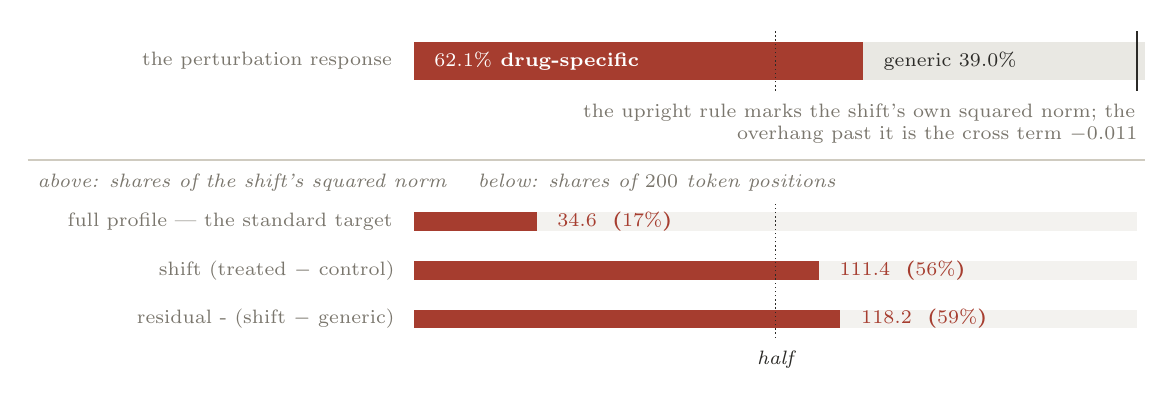
\begin{tikzpicture}[x=1cm, y=1cm, font=\small]
  \def\X{4.900}                  % left edge of every bar
  \def\L{9.190}                  % bar length for 100%
  \newcommand{\bx}[1]{\X+#1*\L}  % value -> x   (no braces: see header)
  % PIN THE BOUNDING BOX. Left free, the picture measures 409.59pt and runs
  % 5.56pt over the block: the rowname nodes are anchor=east at 4.75 with a
  % 4.65cm text width, so their inner sep hangs ~0.09cm left of x=0, and the
  % "half" descender hangs below. Neither carries ink -- the row labels are
  % flush right and set single-line, so their ink starts at x=0.07cm. Pinning
  % to [0, \bx{1.011}] therefore clips nothing and makes the drawn width equal
  % the stated 14.191cm = 403.775pt exactly.
  \useasboundingbox (0,-0.25) rectangle ({\bx{1.011}},4.12);
  \tikzset{
    rowname/.style={anchor=east, text width=4.65cm, align=flush right,
                    font=\scriptsize, text=quietink},
    inlab/.style={anchor=west, font=\scriptsize\bfseries, text=white},
    outlab/.style={anchor=west, font=\scriptsize\bfseries, text=accent},
    greylab/.style={anchor=west, font=\scriptsize, text=ink}}

  % ========== SUB-BLOCK 1: the response, by squared norm. Bars 4.8mm. ======residuak
  \node[rowname] at (4.75,3.70) {the perturbation response};
  \fill[accent]      (\X,3.46)          rectangle (\bx{0.621},3.94);
  \fill[rulegrey!45] (\bx{0.621},3.46)  rectangle (\bx{1.011},3.94);
  \node[inlab]   at ({\X+0.14},3.70)          {$62.1\%$ drug-specific};
  \node[greylab] at ({\bx{0.621}+0.14},3.70)  {generic $39.0\%$};

  % the shift's own squared norm, and the cross term as the overhang past it
  \draw[ink, line width=0.7pt] (\bx{1.0},3.32) -- (\bx{1.0},4.08);
  \node[anchor=north east, text width=7.6cm, align=flush right,
        font=\scriptsize, text=quietink] at ({\bx{1.011}},3.28)
    {the upright rule marks the shift's own squared norm; the overhang past it
     is the cross term $-0.011$};

  % --- the divider: the two sub-blocks are different quantities ------------
  \draw[rulegrey, line width=0.4pt] (0,2.44) -- ({\bx{1.011}},2.44);
  \node[anchor=north west, font=\scriptsize\itshape, text=quietink] at (0,2.38)
    {above: shares of the shift's squared norm \quad below: shares of $200$
     token positions};

  % ========== SUB-BLOCK 2: the target, by token position. Bars 2.4mm. ======
  % r1 -- the standard target
  \fill[rulegrey!25] (\X,1.54) rectangle (\bx{1.0},1.78);
  \fill[accent]      (\X,1.54) rectangle (\bx{0.17},1.78);
  \node[rowname] at (4.75,1.66) {full profile --- the standard target};
  \node[outlab]  at ({\bx{0.17}+0.14},1.66) {$34.6$ \;($17\%$)};

  % r2 -- the shift
  \fill[rulegrey!25] (\X,0.92) rectangle (\bx{1.0},1.16);
  \fill[accent]      (\X,0.92) rectangle (\bx{0.56},1.16);
  \node[rowname] at (4.75,1.04) {shift (treated $-$ control)};
  \node[outlab]  at ({\bx{0.56}+0.14},1.04) {$111.4$ \;($56\%$)};

  % r3 -- the residual
  \fill[rulegrey!25] (\X,0.30) rectangle (\bx{1.0},0.54);
  \fill[accent]      (\X,0.30) rectangle (\bx{0.59},0.54);
  \node[rowname] at (4.75,0.42) {residual - (shift $-$ generic)};
  \node[outlab]  at ({\bx{0.59}+0.14},0.42) {$118.2$ \;($59\%$)};

  % --- the half-way rule, drawn LAST so the bars do not bury it, and drawn
  % ONLY within the two bar bands so it crosses no prose. See header.
  \draw[ink, line width=0.5pt, densely dotted] (\bx{0.5},3.32) -- (\bx{0.5},4.08);
  \draw[ink, line width=0.5pt, densely dotted] (\bx{0.5},0.18) -- (\bx{0.5},1.90);
  \node[anchor=north, font=\scriptsize\itshape, text=ink] at (\bx{0.5},0.14) {half};
\end{tikzpicture}
\caption[The drug is most of the response, little of the
target]{\captiontitle{The drug is the majority of the perturbation response and almost
none of the standard target's tokens.} Above the rule: the shift's squared
norm decomposes exactly into a drug-specific residual, a generic programme and
a cross term, so $62.1\%$ of what a perturbation does to a cell is specific to
the drug. Below it: of the $200$ positions a cell sentence spends on the
standard target, only $34.6$ carry a different gene for two drugs in the same
context --- the other $83\%$ are the same string. Ranking the same measurement
by signed residual raises that to $118.2$, and at the plate scope this build
trains in the residual row reads $120.3$ ($60\%$). The two halves of the figure
are different quantities, a squared-norm share and a count of token positions;
they share the axis and the half-way rule and nothing else, and no difference
between them is a number. What the picture states is an ordering: the signal is
a majority of the response, the standard encoding exposes a small minority of
it to the loss, and the residual encoding puts the exposed fraction back on the
majority side (\cref{tab:divergence}).}
\label{fig:residual-energy}
\end{fullwidth}
\end{figure}



\paragraph{The second question is whether that majority has to be predicted at all}
The first measurement says the drug-specific part is the larger half of a
perturbation response. It says nothing about whether that part is hard to produce.
A residual could be large and still be a per-drug \emph{constant} --- the same
signature for a given drug wherever it is applied --- in which case it is
reproducible from a table indexed by drug name, with no model, no prompt and no
cell involved. So the second question is how much of the residual is that
constant, and how much of it moves with the context the drug is applied in.

Writing
\begin{equation}
 \resid(d,c) \;=\; \beta(d) \;+\; \kappa(d,c) \;+\; \epsilon,
 \qquad
 \Tcoef \;=\; \frac{\operatorname{var}\beta}{\operatorname{var}\beta + \operatorname{var}\kappa},
\end{equation}
splits the residual into a per-drug constant, a context-specific remainder and
noise. $\beta(d)$ is the drug \emph{main effect} and is what a lookup table
reproduces with no model at all;\seealso{\cref{sec:res-lookup} builds that lookup
and scores it.} $\kappa(d,c)$ is the only component a conditional model could win
on; and $\Tcoef$ is the share of the structured part that the constant carries.
The baseline this sets up is not invented for the occasion. It is DrEval's naive
predictor~\cite{dreval} in transcriptomic space: their
\texttt{NaiveMeanEffectsPredictor} predicts $\hat{y}_{ij} = \mu^c_i + \mu^d_j -
\mu$, cell-line and drug main effects with no interaction term, and
$\textrm{generic}(c) + \beta(d)$ is that quantity lifted from a scalar potency to a
$946$-dimensional profile. Asking what $\kappa$ holds is therefore asking what a
model could add over the field's own no-skill predictor.

\paragraph{The direct estimator is unavailable, and what replaces it}
Fitting the variance components would be the obvious route: estimate
$\operatorname{var}\beta$ and $\operatorname{var}\kappa$ and read $\Tcoef$ off
them. It cannot be done on this cache. Separating $\operatorname{var}\kappa$ from
$\operatorname{var}\epsilon$ needs two independent measurements of the same drug in
the same context, and $\num{286}$ of the $\num{287}$ distinct treatments here occur
in exactly one well, so the model is unidentified on its own data. The route taken
instead buys identification from a quantity already computed for the reliability
line. Two residuals of one drug in two cell lines are compared by cosine; that
cosine is depressed by measurement noise in both, and dividing by the geometric
mean of the two conditions' split-half reliabilities removes the depression.

% PLACEMENT: this box carries a display equation and cannot break usefully. At
% the previous setting it opened at the foot of the page and tcolorbox broke it
% immediately after the title bar, stranding "DEFINITION The transfer
% coefficient" alone at the page bottom with every line of the body overleaf.
% \budgettick's own \needspace{5\baselineskip} is not enough to catch that; the
% box is ~13 lines tall, so ask for that and let it move whole.
\needspace{12\baselineskip}
\begin{defn}{The transfer coefficient}
With $\num{286}$ of $\num{287}$ treatments in exactly one well there is
no replicate from which to separate $\operatorname{var}\kappa$ from
$\operatorname{var}\epsilon$, so the variance-components model is unidentified on
its own. The cosine route buys identification through split-half reliability:
\begin{equation}
 \hat{\Tcoef} \;=\; \frac{\cos\!\big(\resid(d,c_1),\, \resid(d,c_2)\big)}
 {\sqrt{\rho(d,c_1)\,\rho(d,c_2)}},
 \qquad
 \rho(d,c) \;=\; \frac{2\cos(\resid_A, \resid_B)}{1 + \cos(\resid_A, \resid_B)},
\end{equation}
where $\resid_A$ and $\resid_B$ are disjoint halves of condition $(d,c)$ and
$\rho(d,c)$ is the Spearman--Brown reliability of that condition's residual at
its full cell count.
\end{defn}

We name explicitly two terms in the formula. The
\emph{cross-line cosine} is the numerator alone: $\cos(\resid(d,c_1), \resid(d,c_2))$,
the plain cosine similarity between one drug's two full residuals in two different
cell lines, computed with nothing else applied to it. \emph{Disattenuation} is a
correction, not a description, and it targets a specific bias. Each residual
entering that cosine is itself a noisy estimate --- it carries the same sampling
error the reliability line was built to detect --- and noise in two vectors being
compared pulls their cosine toward zero independently of whatever the vectors
would agree on if measured exactly. So the raw cross-line cosine understates the
true agreement between contexts by an amount set by how noisy each residual is,
and it understates it more where reliability is lower. Dividing by
$\sqrt{\rho(d,c_1)\,\rho(d,c_2)}$, the geometric mean of the two conditions' own
split-half reliabilities, removes exactly that shrinkage: this is the classical
correction for attenuation, applied here to a cosine instead of the correlation
coefficient it was derived for.\seealso{\cref{sec:appendix}'s planted-truth check
licenses using it on a cosine} $\hat{\Tcoef}$ is what the formula returns after
that division, and calling it \emph{disattenuated} names the correction it has had
applied, not a new quantity being introduced.

Whether the correction actually removes the shrinkage, rather than just
relabelling it, is checkable, because a case exists where the true answer is
known. Data were simulated with $\kappa = 0$ built in --- every context gets the
same residual for a given drug, so by the definition of $\Tcoef$ the truth is
exactly $1$. Measurement noise is simulated too, so the raw cross-line cosine on
this synthetic data still comes out below $1$: it reads $0.734$, which a reader
taking it at face value would misread as $27\%$ context-specific structure,
$1 - 0.734$, when by construction there is none. Dividing that same $0.734$ by
the geometric-mean reliability recovers $\hat{\Tcoef} = 1.001$
(\cref{tab:tcontrols}), against a truth of $1$. The correction is therefore shown
to work on a case where the answer is known, not merely assumed to work because
the derivation is standard, and every number below rests on that check.

\paragraph{What the coefficient is, and what it is not} Four qualifications attach
before any estimate is quoted, and together they make $\Tcoef$ a descriptive
sensitivity analysis rather than a fundamental measurement. First, $\kappa$ is
written as a drug\,$\times$\,cell-line interaction because the decomposition
assumes one, but the estimator does not identify such a term; $\kappa$ is therefore
called the \emph{context-specific remainder} and $\Tcoef$ a disattenuated
cross-context residual-similarity coefficient, never a variance share. Second, it might be tempting to read $1 - \Tcoef$ as the headroom above the constant baseline, however we advise against that: the cross-line pairs
entering it may differ in dose and in treatment well, so it mixes several
axes into one number. Third, the scoped calculation retains conditions at a
reproducibility threshold of $0.2$ and takes each residual against a
\emph{self-including} generic its own drug helped define, which is not the training
frame. Fourth, the reliability in the denominator is a within-well split-half
precision, optimistic relative to biological reproducibility --- and that optimism
has a direction. An over-large $\rho$ makes $\hat{\Tcoef}$ too small, so
$1 - \hat{\Tcoef}$ errs \emph{high} and bounds from above what a per-drug constant
leaves on the table, without measuring it.

One further caution is methodological rather than interpretive. Spearman--Brown is
derived for correlations between parallel halves, not for cosines, and what
licenses its use here is the planted-truth validation of \cref{sec:appendix}.


% ...........................................................................
% ...........................................................................
\begin{table}[htbp]
  % MARGINALIA: in-column; caption and the note in the margin.
  \begin{lrbox}{\tvfb}
  \begin{tabularx}{\textwidth}{@{}Y r l@{}}
  \thead{Quantity} & \thead{Value} & \\
  \midrule
  ground truth, by construction ($\kappa = 0$) & $\Tcoef = 1.000$ & \\
  \addlinespace[10pt]
  uncorrected cross-line cosine, $\cos(\resid(d,c_1), \resid(d,c_2))$ & $0.734$ & \\
  that cosine read naively as an interaction share, $1 - 0.734$ & $27\%$ & (truth:
    $0\%$) \\
  \addlinespace[10pt]
  disattenuated estimator, $\hat{\Tcoef}$ & \key{$1.001$} & \\
  \end{tabularx}
  \end{lrbox}
  \sidecap{table}{\captiontitle{The disattenuation correction, checked where the truth is
  known.} Residuals were simulated with $\kappa = 0$ built in, so by the
  definition of $\Tcoef$ the ground truth is exactly $1$; every row is computed on
  that synthetic data, not on the atlas.\label{tab:tcontrols}
  \par\addvspace{6pt}Measurement noise alone, with no cross-context difference anywhere in the
  simulation, is enough to pull two identical residuals' cosine down to $0.734$.
  The correction recovers the true value to within $0.001$ and licenses the
  reference column of \cref{tab:transfer}.}
  \end{table}

% ...........................................................................
\begin{table}[htbp]
% MARGINALIA: in-column; caption in the margin.
\begin{lrbox}{\tvfb}
\begin{tabularx}{\textwidth}{@{}Z{1.12} r l Z{0.88}@{}}
\thead{Quantity} & \thead{Estimate} & \thead{$95\%$ interval} & \thead{Reference} \\
\midrule
$\Tcoef$ (cross-context, plate-scoped generic) & $0.553$ & $[0.514, 0.593]$
  & simulated $\kappa{=}0$ null $= 1.001$ \\
similarity scale NOT shared across contexts, $1-\Tcoef$ & $44.7\%$
  & $[40.7\%, 48.6\%]$ & mixes cell line, dose, well and estimator \\
\addlinespace[10pt]
$\Tcoef$ across dose (same drug, same line) & $0.707$ & $[0.632, 0.782]$
  & reference scale \\
\addlinespace[10pt]
structure-matched negative control & $-0.008$ & spanning zero
  & must be $\approx 0$ \\
\end{tabularx}
\end{lrbox}
\sidecap{table}{\captiontitle{The transfer coefficient, estimated on real molar doses with
dyadic cluster-robust intervals.} The matched negative control sits on zero. The
same-plate control that produced the earlier false alarm reads $+0.485$ under a
cell-line-scoped generic. $\Tcoef$ is a cross-context similarity coefficient, not
a variance share, and $1 - \Tcoef$ must not be read as a
drug\,$\times$\,cell-line interaction share.\label{tab:transfer}}
\end{table}
\paragraph{What the estimate says} Two things about how this number was obtained
are worth restating before it is read. \emph{Real molar doses}: the dose entering
this calculation is the resolved concentration of \cref{sec:methods-data},
recovered from \texttt{drugname\_drugconc}.
\emph{Dyadic cluster-robust}: $\hat{\Tcoef}$ is computed over \emph{pairs} of
conditions, and two pairs sharing either a drug or a cell line are not
independent observations, so the interval is not a plain bootstrap over pairs
but the Fafchamps--Gubert dyadic estimator of \cref{sec:apparatus-clusters},
built for exactly that dependence.

Under that estimator, on real doses, $\hat{\Tcoef} = 0.553$ $[0.514, 0.593]$
(\cref{tab:transfer}). Read with every qualification above in force: a little over
half of the cross-context similarity scale is carried by the per-drug constant,
and $44.7\%$ $[40.7\%, 48.6\%]$ of it is not.

That reading rests on the negative control holding, so the control is worth
describing rather than only quoting. It is built by keeping everything the
estimand depends on fixed --- the same pair of cell lines, the same plate-scoped
generic, the same disattenuation --- and breaking only the one thing $\hat{\Tcoef}$
is supposed to measure: which drug is compared. Two \emph{different} drugs' residuals
are compared across the same cell-line pair instead of one drug's two residuals,
so any structure the control still detects would have to come from the pipeline
itself, the generic construction or the dyadic clustering, and not from drug
identity. It returns $-0.008$, an interval spanning zero. Nothing in the
construction manufactures apparent cross-context agreement on its own; what
$\hat{\Tcoef} = 0.553$ measures is therefore attributable to the shared drug, not
to an artifact of how the estimator is built.

There is consequently a conditional target that a per-drug constant does not
express, and its size is bounded from above at roughly $45\%$ of a similarity
scale --- not a variance share, and not a quantity any model has been shown to
reach.

\paragraph{Dose is the milder perturbation} The estimand $\hat{\Tcoef}$ is meant
to say how much of the context-specific remainder survives a change of
\emph{cell line} specifically, but the cross-context pairs computing it also
differ in well and, since doses are not matched across cell lines, in dose ---
so the $44.7\%$ that does not transfer could in principle be about that mixture
rather than about cell-line context as such. Dose supplies a cleaner comparison,
because it is the one axis that can be varied while everything else the
estimand depends on --- same drug, same cell line, same generic, same
disattenuation --- stays fixed. If a drug's residual moved as much between two
of its own doses as it does between two cell lines, cell line would be doing no
special work; if it moved much less, dose would be shown to be the milder
perturbation, and the part of the cross-context estimate that dose alone could
explain away would be small.

Holding drug and cell line fixed and varying only the molar concentration,
$\hat{\Tcoef} = 0.707$ $[0.632, 0.782]$ on $\num{363}$ pairs, against
$\hat{\Tcoef} = 0.553$ $[0.514, 0.593]$ pooled across cell lines; the intervals
do not overlap. Dose is therefore the milder perturbation: a drug's residual
survives a change of concentration better than it survives a change of cell
line, so the $44.7\%$ that does not transfer across context is not merely an
artefact of comparing different doses to each other. The comparison is not
perfectly clean --- the cross-context arm still differs in well and dose as well
as cell line, so this is the closest the section comes to a single-axis test
rather than one --- but the direction runs the way the estimand's own logic
predicts.


 
\paragraph{Whether anything could learn the remainder} The $44.7\%$ a per-drug
constant does not reach is not automatically a target only a full model could
hit. A simpler explanation is available first. If a cell line modulated every
drug's response in a broadly consistent direction --- a ``cell-line
personality'' that is not any drug's own signal but is nonetheless learnable
from that line's other conditions --- then two \emph{different} drugs measured
in the \emph{same} cell line should share more of that direction with each
other than either shares with a drug measured in a \emph{different} cell line,
once each drug's own main effect is removed. That prediction is specific enough
to test directly.

Testing it means removing the main effect first. Write
$\kappa(d,c) = \resid(d,c) - \hat{\beta}(d)$, where $\hat\beta(d)$ is estimated
\emph{leave-one-cell-line-out}: averaged over every cell line except $c$, so
condition $(d,c)$ never enters its own baseline. That exclusion is not a
formality. Estimated over every line including $c$, $\hat\beta(d)$ would
contain $\resid(d,c)$ itself, and centring a value on a mean that contains its
own contribution induces a $-1/(m-1)$ correlation between the centred values by
the arithmetic of the mean alone, before any real structure enters ---
precisely the leave-one-out concern already argued for the generic in
\cref{sec:methods-residual}, protecting a variance test here rather than a
training target. With the main effect removed, the test compares two cosines:
$\cos(\kappa(d,c), \kappa(d',c))$, two different drugs' remainders in the same
cell line, against $\cos(\kappa(d,c), \kappa(d',c'))$, two different drugs in
two different cell lines. A cell-line personality predicts the first running
higher than the second. Both cosines are disattenuated by $\kappa$'s own
split-half reliability before the comparison is made, for the same reason
$\hat{\Tcoef}$ itself is: an uncorrected cosine would read the personality's
absence as smaller than it is, purely because $\kappa$ is a noisier quantity
than $\resid$.

Averaged over lines, neither arm shows the signature the hypothesis predicts.
Under the plate-scoped generic the same-cell-line arm reads
\ci{-0.0149}{-0.0251}{-0.0050} and the different-cell-line arm
\ci{+0.0003}{-0.0071}{+0.0081}, an excess within line of $-0.0153$ for which no
interval was computed; both come from a cell-line-clustered bootstrap,
$\num{38}$ and $\num{42}$ clusters respectively, over $\num{4000}$ same-line and
$\num{3884}$ cross-line pairs drawn from $\num{1282}$ conditions. A real
per-line direction predicts the same-line arm sitting \emph{above} the
cross-line one; instead it sits below it, and it is the only one of the two
distinguishable from zero at all. That negative same-line reading is not itself
read as evidence of some opposite structure, because it has a known
non-biological cause: same-line pairs that also share a plate share a generic,
and subtracting one shared quantity from both members of a pair pushes their
cosine negative by construction --- the identical mechanism the different-drug
same-plate diagnostic reads at $-0.017$ elsewhere in this section. Cross-line
pairs share no generic and are unaffected by it. So the uncontaminated arm is
the cross-line one, and it is indistinguishable from zero, while the same-line
arm's departure from zero is explained by the construction rather than by any
drug-independent cell-line effect. Neither arm, then, shows the positive
within-line excess a consistent per-line direction would require. 


% ...........................................................................
\beatsection{R}{5}{Re-encoding produces prompt sensitivity}{sec:res-encoding}

\begin{question}[5]
Every target change tried so far has not shown robust counterfactual predictions. Does training on the residual change that? The instrument is the
stratified scramble, the same prompt with another drug's name and mechanism
substituted, read as a ladder of strata because the swapped-in drug is itself a
drug the model knows and so is not a neutral comparison. The model moves. It is
not the only target change that makes it move.
\end{question}

\noindent

Every scramble so far has been run on \texttt{tier2}: held-out drugs, ones the
checkpoint never saw in training, with the substituted partner drawn from that
same held-out set. That is a hard test and deliberately so, but it asks for two
things at once. A model that passes it must respond to the drug it is named
\emph{and} have learned something transferable about a drug it has never
encountered. Nothing has passed it. The single-cell arm is null under the
random-partner comparison and shows no ordering under its own designed sweep;
consensus is flat at every swap distance; optimal transport clears zero only
against the most dissimilar partners and nowhere before them.

This section separates the two demands and asks only the first. The ablation is
unchanged. Same prompt, same substitution, same comparison set, but it is
run on conditions the residual checkpoint actually trained on,and, for the two
controls, on a sample whose split its evaluation did not record --- so that for at
least the arm this section is about, nothing has to be extrapolated and
memorisation is available. That makes it the easier question by
construction, and the right one to ask next: if a model is sensitive to the drug
token at all, this is where it shows, and a null here would be much harder to
attribute to the difficulty of the split.

It also brings in a fourth target. The residual re-encoding of
\cref{sec:methods-residual} was not among the three constructions of
\cref{sec:res-epsilon}; it is what this section is about, and two of those three
are carried forward with it --- but not as a yardstick. Relaxing the split is a
concession, and the obvious objection to anything found after making it is that
the concession \emph{is} the finding: that scoring a model on conditions it has
already fitted is by itself enough to open a gap against a scrambled prompt. The
controls are here to answer that objection, not to compete for a ranking. They are
read out of the same evaluation cache, through a ladder built by the same rule,
against the same kind of comparison. One thing about them has to be said straight
away, because it bounds what they can settle: their evaluations carry no split
manifest, so which of their conditions each checkpoint had already seen is not
recorded, and they cannot certify that the relaxation was granted to them on the
same terms. What they do bound is the instrument --- whether this ladder, read out
of this cache, returns a large positive gap as a matter of course --- and that is
the reason they are drawn. No ordering between arms is claimed anywhere below.

Carrying them forward also fixes where the earlier nulls do \emph{not} come from,
and the two controls answer that differently. \Cref{sec:res-blind} and
\cref{sec:res-epsilon} found neither construction able to order its gap by swap
distance on held-out drugs, scored in the expression frame they were trained to
emit --- flat throughout for single cell, and for optimal transport a single
narrow excursion at the far end and nothing before it. Read here on seen conditions and
in the residual frame, the single-cell arm is still not recovered: its series spans zero
at every stratum. Neither control's split is recorded, so that is not the clean
seen-condition null it would be worth having; what it does establish is narrower
and still useful: pointed at this checkpoint, on this cache and this ladder, the
instrument returns nothing at all, so it does not open a gap merely by being run. Optimal
transport is partly recovered, and that is the second reason to draw it. Its
\texttt{orth} and \texttt{opposite} gaps both clear zero here, small but real, and
this section is where the reading that that arm does nothing is withdrawn. The
withdrawal is budget-driven and internal to this instrument: on the same
checkpoint against the same \texttt{orth} comparator, $600$ tokens give
\ci{+0.0144}{-0.0032}{+0.0323}, spanning zero, and $1400$ give
\ci{+0.0292}{+0.0144}{+0.0441}, which does not --- though on a pool sharing only
$\num{10}$ conditions with the first. It is not a re-run of
\cref{sec:res-epsilon}'s own sweep, which is a different frame, population and
comparator; what it withdraws is that sweep's conclusion, not its number. What it still does not show is ordering across the
ladder, and the limits below are explicit that this is a statement
about the ladder its pool supports rather than about the arm. Neither reading
turns on a comparison with the residual arm, and
\cref{sec:res-generalisation} is where the harder question goes back to whichever
arm survives this one: whether the response holds on conditions never trained
on.

One consequence of that relaxation belongs up front, before any design detail or
any number: the arms are no longer scored on a common set. Each is read on a
scoring sample of a few hundred conditions rather than a full population, since
three scrambled generations per condition is expensive, and those samples were
drawn separately --- three pools in all: one $\num{250}$-condition pool, shared by
all three arms at $600$ tokens and reused for the pre-repair checkpoint at
$1400$; the repaired residual arm's $\num{300}$ at $1400$; and the controls'
$\num{248}$ at $1400$. At $1400$ the two are mostly non-overlapping
and they differ in size. What is held fixed is not the
data but the shape of the instrument: the near/orth/opposite ladder below is
built the same way wherever it is built, so the only reading any of it supports
is an arm against its own scramble on its own conditions, never one arm's number
against another's.

The instrument itself needs one design choice made explicit before any number is
worth reading. For each condition, a partner drug is drawn from every other
condition sharing its cell line \emph{and} its plate but naming a different drug
--- same plate so a swap never differs from the target in batch as well as in
identity, different drug so a drug's own other dose is never mistaken for a
scramble --- and three fixed partners are taken from that pool by measured
residual cosine: the \emph{near} partner is the most similar available,
\emph{orth} the one closest to orthogonal, \emph{opposite} the most
anti-correlated. The pool is ranked by residual cosine and not by the
\texttt{moa-fine} mechanism annotation because the annotation does not track it:
two drugs sharing a mechanism label sit a mean distance $2.322$ apart against
$2.377$ for two that do not ($\num{1244}$ same-mechanism against $\num{17563}$
different-mechanism pairs, from the drug atlas of \cref{sec:apparatus-vocab}), just over two per cent closer,
so ``different mechanism'' does not imply ``different response''. A condition
with fewer than three eligible partners is dropped rather than assigned a
contaminated one. The three partners are fixed by this construction and reused, unchanged, across
every arm scored within one evaluation run --- though not across runs: the
$1400$-token control run draws on a different pool, whose \texttt{opposite} rung
is much the weaker of the two, as \cref{fig:repair} sets out.

On a scoring sample of $\num{300}$ conditions the holdout assigns to
\texttt{train}, $\num{293}$ of which the evaluation also flags as seen --- the
\texttt{train} tier of the three-way holdout \cref{sec:methods-residual} builds,
scored on that same checkpoint's evaluation (\texttt{re\_v3.json}, one
generation budget of $1400$ tokens throughout, the only budget this checkpoint
has been scored at) --- the model separates from its own scramble on two of the
three partners, and moves in the predicted direction on the third, in the order
the construction predicts throughout. Against \texttt{near}, the hardest test,
the gain is smallest and does not clear zero,
\ci{+0.0229}{-0.0232}{+0.0689}; against \texttt{orth} it is
\ci{+0.0898}{+0.0382}{+0.1415}, clustered on cell line and well
(\ci{+0.0898}{+0.0291}{+0.1506} clustered on drug and well); against
\texttt{opposite} it more than doubles again,
\ci{+0.1942}{+0.1358}{+0.2527}.\gloss{scramble}{The same prompt with the drug's
name and mechanism replaced by another drug's, in three strata by residual
similarity.} One checkpoint, one evaluation, one generation budget, one
population: on the conditions this checkpoint was trained on, the model separates
from its own scramble in the order the construction predicts, and it is not the
only target construction that separates at all.

 % ...........................................................................
% ...........................................................................
\paragraph{Why three strata, and why one of them is quoted} The three strata are
not three attempts at the same measurement. They are three detection
sensitivities, set deliberately. Every prediction is scored against the
\emph{real} drug's truth, so what changes across the strata is not how hard the
prediction is to produce but how visible it is that the model followed the drug
it was named. Substitute a near-twin and an unchanged prediction is nearly the
correct answer anyway, so the scramble scores well and there is almost nothing
to see. Substitute an opposite effect drug and a model that actually follows its
prompt is pushed away from the truth in the one direction the metric measures,
so the scramble collapses and the separation is at its widest. The model's own
score is fixed at $0.598$ throughout; it is the scramble NIR across the stratum that falls, $0.575$
to $0.508$ to $0.404$, and the gap that opens with it. A model doing genuine
counterfactual work should therefore separate most on \texttt{opposite} and
least on \texttt{near}, which is the ordering \cref{tab:reencode-gradient}
reports. That ordering is the evidence. A metric artefact, or a model
reproducing a generic response regardless of the drug, has no reason to arrange
itself by how dissimilar the substituted drug happens to be, so the shape of the
series across strata says something no single stratum can.

A single number is nonetheless needed, and not for anything internal to this
section: everything downstream requires one. Reporting an arm compactly means one figure per
arm, not three; \cref{sec:res-generalisation} compares the trained tier against
two held-out ones, and its evaluation was run against one fixed comparator
(\texttt{scramble\_orth}) rather than re-run three times; and every later section
that cites this effect --- the lookup-table comparison, the channel gate, the
chapter summary --- inherits whatever one quantity is named here. The choice is
therefore about which stratum's gap can honestly carry the label ``the effect''.

\texttt{Orth} is the only candidate, and the reason is that it alone has a
defensible null. Scored on its own, the \texttt{near} partner reaches $0.575$,
above the $0.500$ chance line: naming a similar drug is partly \emph{correct},
so a gap measured against it subtracts real signal and understates the effect.
The \texttt{opposite} partner scores $0.404$, below chance: that substitution is
actively wrong, so a gap measured against it inflates. \texttt{Orth} sits at
$0.508$, on the chance line almost exactly, which is what makes its gap read as
distance above chance rather than distance from a contaminated baseline. Reading
the three partners as points on one line rather than as three separate
comparisons makes the same point: their own scores fall monotonically with the
cosine between the substituted drug's truth and the real one, and \texttt{orth}
is where that line crosses chance. It is the one place on the ladder where
subtracting the comparator neither gives the model credit for a partly right
answer nor charges it for a wrong one.

% ...........................................................................

% ...........................................................................
% ...........................................................................
% ...........................................................................
\paragraph{How the scoring sample is built for each arm, and what makes the
three comparable} 
Nothing here is scored on a full population. For each arm, a
\emph{scoring sample} is drawn from the evaluation cache, for the residual arm
from conditions it had already seen during its own training --- a few hundred conditions, not the whole set --- and every
number in this section is read off that sample. The residual arm's is the
$\num{300}$-condition \texttt{train} tier of the three-way holdout
\cref{sec:methods-residual} builds, and its trained status is recorded per
condition. The two controls are read on one shared sample at each budget --- $\num{250}$
conditions at $600$ tokens and a near-disjoint $\num{248}$ at $1400$, with only
$\num{10}$ conditions common to the two --- drawn from the same evaluation cache
the residual arm is itself scored out of. Neither control evaluation carries a
split manifest; both record the split as unknown for every condition, so which of
them each checkpoint had already trained on is not established. Their rows are
nulls of unverified split rather than demonstrated seen-condition nulls, and the
seen-condition framing of this section is secure only for the residual arm, whose
$\num{300}$ come with the three-way holdout attached.

The three samples are not three views of one population, and this is the point
worth being plain about: the three arms were trained on different data. Each
target construction came with its own corpus, built at its own time, under its
own inclusion rules, and no arm was retrained to match another's. A scoring
sample drawn this way therefore means a different set of conditions
for each arm, and the samples differ in size as well: the residual arm's
$\num{300}$ and the controls' $\num{248}$ have just $\num{15}$ conditions in
common. Nothing survives that in the form a cross-arm comparison would need. What
each sample does support is one arm read against its own scramble on its own
conditions, and that is the only reading taken below. 

% ---------------------------------------------------------------------------
\begin{table}[htbp]
% MARGINALIA: full width, like the other interval tables of this section;
% caption above at the text width, notes below in the sans.
\caption{\captiontitle{On the conditions the checkpoint trained on, the gap runs from
a partly-correct partner to an actively wrong one, at one checkpoint and one
generation budget.} Model $\NIR$ is $0.598$ in every row; only the comparator
changes. \texttt{re\_v3.json} / \texttt{scramble\_stratum\_audit\_v4.json},
$n = \num{300}$ throughout.}
\label{tab:reencode-gradient}
\begin{fullwidth}
\begin{threeparttable}
\begin{tabular}{@{}l l r r r l@{}}
\thead{Stratum} & \thead{Partner is} & \thead{Partner cos.} & \thead{Scramble NIR}
  & \thead{Gap} & \thead{$95\%$ interval (cell line, well)} \\
\midrule
\arm{near} & most similar available & $+0.248$ & $0.575$ & $+0.023$
  & $[-0.023, +0.069]$ \\
\arm{orth} & closest to orthogonal & $-0.0001$ & $0.508$ & \key{$+0.090$}
  & $[+0.038, +0.142]$ \\
\arm{opposite} & most anti-correlated & $-0.261$ & $0.404$ & $+0.194$
  & $[+0.136, +0.253]$ \\
\end{tabular}
\begin{tablenotes}[flushleft]
\item Partner cosine is the mean cosine, in the residual frame, between a
condition's own residual and the partner substituted for that row's stratum. Scramble NIR is the NIR of the prediction when swapping the name of the drug with that of what is in the stratum(near,orth,opposite).
The \texttt{orth} row additionally excludes zero clustered on drug and well,
\ci{+0.0898}{+0.0291}{+0.1506}; no drug-clustered interval was computed for the
other two rows.
\end{tablenotes}
\end{threeparttable}
\end{fullwidth}
\end{table}

% .....................................................................
% RESOLVED IN PROSE (not in data): re_singlecell_1400.json has cache_dir=ot_cache,
% which is NOT the corpus pythia_sft_endcell trained on, so its rows are not a
% verified seen-condition test. Rather than quote numbers under a sampling
% discipline they do not have, the prose above now states this limitation
% outright and marks the single-cell rows as a null of unverified split. If the
% same-corpus rerun on data_diverse2_endcell_big ever lands, swap the numbers in
% that paragraph, the two-panel figure/JSON and ctrl1400_summary.json, and the
% caveat can be deleted.
% Verified 2026-08-30 from the artifacts: re_singlecell_1400.json and
% re_ot_1400.json score the SAME 248 conditions (split='unknown', trained=False,
% train_file=None, holdout=None); those 248 overlap the residual train tier in
% only 15 conditions; repro_cos min 0.2022 / median 0.2784 for the 248 against
% 0.1089 / 0.1827 for the residual 300 --- i.e. the controls' pool is the more
% reliable one, so the reliability filter is NOT a confound favouring the
% residual arm.

% ...........................................................................
\paragraph{Two controls, read at both budgets, and one residual cell that is a
different model}
 Every run this section has is in \cref{tab:budget-arms}, and the residual arm
contributes three of them rather than two. Two are the \emph{pre-repair}
checkpoint --- trained on targets built before the split-before-fit correction of
\cref{sec:methods-residual}, when the generic and the reliability filter were
still fitted over every condition and the holdout assigned afterwards --- scored
at both budgets on one $\num{250}$-condition pool. Those two rows are the
chapter's one clean budget comparison: one checkpoint, one pool, one comparator,
with the budget the only thing that moves, and the gap roughly doubling at every
stratum when it does. The third is the repaired checkpoint at $1400$ tokens, which
is where this chapter's canonical result comes from and which has never been
scored at $600$; it cannot be read against either pre-repair row without
confounding a target rebuild with a budget change. The two
control arms have no such problem at the level of the checkpoint: each was scored
at both budgets on its own single checkpoint. Their two budgets are not read on
one condition set, though --- the $600$- and $1400$-token pools share only
$\num{10}$ conditions --- so those rows move budget and population together, and
are not budget comparisons alone.

Read at $1400$ tokens, where the residual arm's canonical checkpoint actually
lives, neither control shows a three-stratum pattern --- though on their pool the
three strata are not three distinct tests, so only the near-versus-rest half of
that is a real null. The
single-cell control is flat and null at every stratum. The optimal-transport
control is not flat, and clears zero on two of the three strata --- but at
\texttt{orth} and \texttt{opposite} almost equally, which on this pool is close to
being the same measurement twice: in $\num{138}$ of its $\num{248}$ conditions the
two strata name the same partner drug. Both arms'
full three-stratum results at both budgets are in \cref{tab:budget-arms}.

One asymmetry in scrutiny attaches to the optimal-transport \texttt{orth} value.
Unlike the residual arm's own headline number, it has not been re-checked under
drug-and-well clustering; the drugs behind those conditions repeat across them
the same way the residual arm's do, so a wider drug-clustered interval is not
ruled out, only untried.

Three limits stop any of this being read as an ordering between arms. The first
is the frame. The residual checkpoint's generations are scored where they are
emitted, while the two controls emit cell sentences, whose decoded profile is a
function of gene rank order alone; a drug effect can reach their gaps only by
reordering top-ranked genes, which is the channel \cref{tab:divergence} measures
as nearly closed --- $34.6$ of $200$ top positions differing between two drugs
under the standard encoding, against $120.3$ under the residual one. Their gaps
are attenuated by construction, and an attenuated gap cannot be read against a
native one.

The second is that the ladder is not equally built in the two pools, and this is
measurable rather than a matter of interpretation. Across the residual arm's
$\num{300}$ conditions, every \texttt{opposite} partner is a different drug from
that condition's \texttt{orth} partner, and all $\num{300}$ opposite cosines are
negative, mean $-0.261$. Across the controls' $\num{248}$, \texttt{opposite} and
\texttt{orth} name the \emph{same} drug in $\num{138}$ of them --- $\num{56}\%$
--- and only $\num{133}$ of the opposite cosines are negative at all, mean
$-0.009$. The controls' top two rungs are largely one rung, which is the plainest
reading of why their \texttt{orth} and \texttt{opposite} gaps come out almost
equal, and it means an absence of near-to-opposite ordering in those arms is not
evidence that they lack it: the instrument that would have shown it was not there
to be failed.

The third is that these are separate evaluations over different, mostly
non-overlapping condition sets drawn from separately built corpora, not a paired
comparison, and the arms were not held to the same training discipline.

One thing that could have been a further limit is not one, and it is worth saying
so rather than leaving it to be assumed. The residual arm's $\num{300}$ conditions
are the reliability-surviving population of \cref{sec:methods-residual}, which
invites the objection that its result is a property of a pre-screened sample. The
controls' $\num{248}$ are the more reliable pool of the two, not the less: their
lowest reproducibility cosine is $+0.202$ against the residual tier's $+0.109$,
their median $+0.278$ against $+0.183$. Whatever this section's numbers are, they
are not the product of the residual arm having been handed the easier
conditions.

A pattern that survives the sharpest stratum on one arm is evidence about that
arm. Its absence on an arm whose sharpest stratum was never built is not evidence
about that one, and neither fact is a ranking. The comparative case in this
chapter is not made in this section at all: it is made by \cref{tab:divergence},
which counts how far two drugs' target strings diverge under each encoding and
needs no model to do it.
\begin{figure}[htbp]
\begin{fullwidth}
  \raggedright
  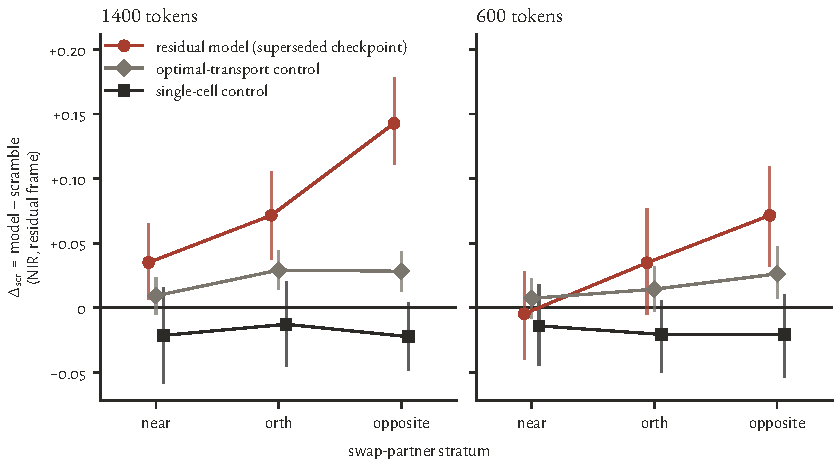
\includegraphics{fig-repair}
  \caption[Budget, not target, moved this gap]{\captiontitle{Raising the generation
  budget from $600$ to $1400$ tokens sharpened a real pattern rather than
  manufacturing one: the residual checkpoint's advantage over its own scramble
  grew at every stratum, the optimal-transport control's grew from
  null-adjacent to clear, and the single-cell control stayed flat at both.}
  Residual frame throughout; the optimal-transport and single-cell series are the
  \emph{implied} residual described above, since neither checkpoint was trained
  to emit one. Both panels share the residual checkpoint's superseded, pre-repair
  run, the only one with a $600$-token measurement; the current checkpoint's
  canonical result (\cref{tab:reencode-gradient}) is not drawn here. The $x$-axis
  is the stratum by name, not by measured cosine: at $600$ tokens all three series
  share one $250$-condition partner pool (mean residual cosine $+0.406$,
  $-0.0016$, $-0.329$ for near, orth, opposite); at $1400$ tokens the residual
  series keeps that same pool while the two controls were scored on a different,
  smaller $248$-condition pool whose near and orth partners shift by less,
  $+0.403$ and $+0.036$, but whose \texttt{opposite} partner is only weakly
  anti-correlated, $-0.009$, so the two panels' \texttt{opposite} points are not a
  matched pair. Intervals are $95\%$ bootstrap, $n = 250$ per point at $600$
  tokens and $n = 248$ at $1400$ for the two controls; clustering differs by
  series and is not uniform across this figure --- the two controls' $1400$-token
  intervals are clustered on cell line and well, matching the number quoted for
  them in the text, while every other series here (the residual arm at both
  budgets, both controls at $600$) has only a coarser cell-line-only interval
  computed and is plotted with that instead.}
  \label{fig:repair}
\end{fullwidth}
\end{figure}
% ---------------------------------------------------------------------------
\begin{table}[htbp]
  % MARGINALIA: full width; caption above at the text width, notes below.
  % Every interval sits in an l column so it never breaks mid-cell.
  \caption{\captiontitle{Every arm at both generation budgets, model minus its own
  stratum-matched scramble.} The four control rows hold one checkpoint each across
  the two budgets, but not one condition set: the $600$- and $1400$-token pools
  share only $\num{10}$ conditions. The two pre-repair residual rows are the
  cleanest pair here --- one checkpoint, one $\num{250}$-condition pool, budget the
  only thing that moves. The repaired row is a different checkpoint from those two,
  so reading it against them would mix a target rebuild with a budget change.}
  \label{tab:budget-arms}
  \begin{fullwidth}
  \begin{threeparttable}
  \begin{tabular}{@{}l r r l l l@{}}
  \thead{Arm} & \thead{Budget} & \thead{$n$}
    & \thead{near} & \thead{orth} & \thead{opposite} \\
  \midrule
  \arm{residual, repaired}\tnote{a} & $1400$ & \num{300}
    & \ci{+0.023}{-0.023}{+0.069}
    & \key{\ci{+0.090}{+0.038}{+0.142}}
    & \ci{+0.194}{+0.136}{+0.253} \\
  \arm{residual, pre-repair}\tnote{b} & $1400$ & \num{250}
    & \ci{+0.035}{+0.006}{+0.066}
    & \ci{+0.072}{+0.037}{+0.106}
    & \ci{+0.143}{+0.111}{+0.179} \\
  \arm{residual, pre-repair}\tnote{b} & $600$ & \num{250}
    & \ci{-0.005}{-0.040}{+0.028}
    & \ci{+0.035}{-0.005}{+0.077}
    & \ci{+0.072}{+0.032}{+0.110} \\
  \addlinespace[10pt]
  \arm{optimal transport} & $1400$ & \num{248}
    & \ci{+0.009}{-0.005}{+0.024}
    & \ci{+0.029}{+0.014}{+0.044}
    & \ci{+0.028}{+0.013}{+0.044} \\
  \arm{optimal transport} & $600$ & \num{250}
    & \ci{+0.007}{-0.008}{+0.023}
    & \ci{+0.014}{-0.003}{+0.032}
    & \ci{+0.026}{+0.007}{+0.048} \\
  \addlinespace[10pt]
  \arm{single cell} & $1400$ & \num{248}
    & \ci{-0.021}{-0.059}{+0.016}
    & \ci{-0.013}{-0.046}{+0.020}
    & \ci{-0.022}{-0.049}{+0.004} \\
  \arm{single cell} & $600$ & \num{250}
    & \ci{-0.014}{-0.045}{+0.018}
    & \ci{-0.021}{-0.050}{+0.006}
    & \ci{-0.020}{-0.054}{+0.010} \\
  \end{tabular}
  \begin{tablenotes}[flushleft]
  \item[a] The canonical result, repeated from \cref{tab:reencode-gradient} for
  comparison. It is the only row scored on a population with a split manifest
  attached, and the only one the chapter's claim rests on.
  \item[b] Pre-repair checkpoint, trained on targets built before the
  split-before-fit correction of \cref{sec:methods-residual}, scored at both
  budgets on one $\num{250}$-condition pool. These two rows are the series
  \cref{fig:repair} draws for the residual arm. The repaired checkpoint has never
  been scored at $600$ tokens, and is not drawn in that figure.
  \end{tablenotes}
  \end{threeparttable}
  \end{fullwidth}
  \end{table}

  \paragraph{The slope carries its own null}
  One further check supports reading \texttt{orth} as the honest point on that
ladder, and it does so without selecting any comparator at all. Each condition
contributes three scrambled prompts, and each names a partner drug whose true
residual sits at a measured cosine from the real drug's --- on this tier
$+0.25$, $0$ and $-0.26$ for near, orth and opposite.  Regressing each prompt's $\NIR$ on
that cosine, over all three prompts of every condition at once, asks a question
none of the individual gaps can: does the score track how similar the named drug
actually is? The regression is pooled least squares with one intercept, three
points per condition and no condition-level intercepts absorbed, and the
target-drug prompt is never a point on the line --- only the three scrambles
are, so nothing in the fit contrasts the model against a chosen baseline.

Zero is the null by construction. A model that ignores the drug it is told
emits the same prediction whichever partner is substituted, so its three points
sit at the same height and the line is flat, whatever the partners' cosines
happen to be. On the trained tier the slope is \ci{+0.3728}{+0.2084}{+0.5139}:
positive, excluding zero, and steep enough that moving a partner from
anti-correlated to similar --- a span of roughly $0.5$ in cosine --- buys about
$0.19$ in $\NIR$, which is the same order as the spread between the three
comparator scores the ladder is built from. What that establishes is not
\texttt{orth} directly but the ladder underneath it: the comparators really do
fall in the order their labels claim, and by an amount that scales with the
cosine, so \texttt{orth}'s position at the chance crossing is a property of the
measured geometry and not an artifact of which three partners happened to be
picked. \Cref{sec:res-generalisation} fits the same slope on the two held-out
tiers. One caveat on reading its magnitude rather than its sign: with a single
pooled intercept the zero null is exact within a condition, but the fitted slope
also carries a between-condition component.


\paragraph{Both budgets, side by side} The budget is not a neutral runtime
setting here. Raising it from $600$ to $1400$ tokens moved the
optimal-transport control's \texttt{orth} gap from spanning zero to excluding
it, very nearly doubling the point estimate on an identical checkpoint and an
identically constructed comparator, though on a nearly disjoint sample of
conditions, while leaving the single-cell control null at both budgets --- so
the budget sharpens a gap that is already there and does not manufacture one
where there is none. \Cref{fig:repair} puts all three arms at both budgets side
by side, one panel each, across the three strata;
\cref{tab:budget-arms} carries the same numbers.

The figure's $x$-axis is the stratum by name rather than measured cosine,
because the two panels do not rest on one partner pool. At $600$ tokens all
three arms share a single $\num{250}$-condition pool. At $1400$ the two controls
were re-run on a smaller $\num{248}$-condition pool whose \texttt{opposite}
partner is barely anti-correlated, $-0.009$ against $-0.329$ in the pool the
residual series keeps; near and orth move far less, $+0.406\rightarrow+0.403$
and $-0.0016\rightarrow+0.036$. The controls' $1400$-token \texttt{opposite}
point is therefore a weaker test than any other point on either panel, and
plotting all three series on one continuous cosine axis would draw a shared
difficulty ladder the data does not support.


% ...........................................................................
\beatsection{R}{6}{Responding to the drug is not predicting it}{sec:res-generalisation}
\label{sec:methods-holdout}

\begin{question}[6]
A model that moves when the drug token moves has cleared a low bar, because
reproducing a training average requires that much too. Everything scored so far
came from conditions the model trained on, so what has been shown is that the
token is consulted, not that anything transferable was learned. Separating the
two needs a holdout, and the
atlas's own randomisation decides which one means anything: whole treatment
wells. Prompt sensitivity survives that test. Whether the residual itself
transfers comes back unsettled.
\end{question}

\noindent

\Cref{sec:res-encoding} established one thing, and deliberately only one. On
conditions the checkpoint had trained on, re-encoding the target made the model
respond to the drug it was named: the separation opens in the order the
construction predicts, it holds clustered on the cell line and on the drug, and
the comparator-free slope excludes zero. That was the easy question by design.
Nothing had to be extrapolated, memorisation was available, and a model that did
no more than reproduce a training average would have cleared much of the same bar.
What it establishes is that the prompt is consulted, not that anything was learned
that travels.

Where the response stops is the question worth asking, and this atlas supports two
ways of asking it. One recombines what the model has already met: a trained drug
seen again in a treatment well held out whole. The other withholds the drug from
fine-tuning altogether. The first is the weaker test and the second is the one the
claim has to survive. Both are reported below, and they fail in different places.

The physical layout of \cref{sec:methods-data} forces the choice. A (drug, cell
line) holdout, the field's standard Leave-Pairs-Out split and the one an earlier
version of this work used, leaves the held-out condition's treated well sitting
in the training set through its other $\approx 48$ cell lines. Measured against
that holdout, $\num{124}$ of the $\num{255}$ treated wells for which split
information exists placed a held-out condition and a training condition in the
same well.\seealso{\cref{sec:res-lookup}: what a held-out gap has to
beat.} That estimand measures within-atlas matrix completion, not independent
generalisation, and no processing of the targets changes it.

Holding out whole wells is the only assignment-respecting choice the design
offers, and it answers a narrower question, generalisation to an unseen treatment
well of a seen drug. Fixed-dose cross-context transfer, present in one line and
absent in another, is structurally unidentifiable in this atlas.

\paragraph{What each split holds} \texttt{train} takes every condition of the
remaining wells, $\num{4999}$ before the reliability line and 2,685
after it.
\texttt{unseen\_combo} holds $\num{36}$ treated wells out whole ($\num{904}$
conditions, $\num{900}$ after inventory filters), and it never takes a drug's
last training well; without that guard a two-well drug could silently become an
unseen drug while sitting in the unseen-combination arm, and the two arms would
measure the same thing. \texttt{unseen\_drug} holds every condition of
$\num{10}$ held-out drugs ($\num{714}$ conditions, $\num{711}$ after inventory
filters). Zero wells contribute conditions to both sides.

\texttt{unseen\_drug} is a control and not a third result. Tahoe fine-tuning
never sees the token, so a large effect there would indict the comparator, not
report a biological finding. ``Unseen'' means held out from fine-tuning with
mechanism supplied, not unknown to the pipeline; the Pythia-1b backbone was
pretrained on natural language and the prompt still carries the
\texttt{Mechanism:} field.

Two warnings ride with the design. DrEval reports, citing~\cite{partin}, that
apparently good performance on pair-holdout splits can be reached simply by
predicting each drug's average response across the training cell lines, which is
why the baseline ladder of \cref{sec:res-lookup} is not optional. And the
evaluation draws under a per-split quota, because a uniform draw reproduces the
pool's proportions and starves the split the experiment exists to test; in a
first run,
$\num{250}$ constructed held-out combinations yielded only $\num{33}$ scored
conditions. Under the quota the evaluation scores $\num{1394}$ conditions in all,
$\num{300}$ trained and $\num{199}$ unseen-drug, the rest unseen combinations,
almost the whole pool of $\num{900}$ that arm affords, while
\texttt{unseen\_drug} remains a quota of the $\num{711}$ available.

% ...........................................................................
\paragraph{The first result of this design is about the comparator} Which partner
defines the gap decides the size of every number in this section, and only one of
the three has a claim to the role. A gap splits at chance into how far the model
rises above it when handed the right drug and how far the comparator falls below
it when handed a wrong one,
\begin{equation}
 \gap \;=\; \underbrace{\big(\NIR_{\textrm{model}} - 0.5\big)}_{\textrm{how much naming the truth helps}}
 \;+\; \underbrace{\big(0.5 - \NIR_{\textrm{scramble}}\big)}_{\textrm{how much naming the lie hurts}},
\end{equation}
and only \texttt{orth} makes the second term vanish: its own score is $0.501$,
against $0.550$ for \texttt{near} and $0.423$ for \texttt{opposite}.

That second term is not noise --- it is the model being pushed away from a truth
it was told to miss --- but how far it is pushed depends on which partner the
prompt named. Each condition's three partners are drawn from the other drugs on
its own plate and ranked by the cosine between their true residual and the
target's (\cref{sec:res-encoding}): \texttt{orth} is the partner closest to zero,
and \texttt{opposite} the most anti-correlated available, meaning the drug whose
measured response points most nearly against the target's. That cosine is a fact
about which drugs shared a plate, not about the model, and it does not hold still
across the splits. Averaged over conditions, the \texttt{opposite} partner reaches
$-0.2615$ on \texttt{train} but only $-0.1842$ on \texttt{unseen\_combo}, because
the most anti-correlated drug \emph{available} is whatever happened to be plated
alongside; \texttt{orth} sits within $0.0005$ of zero on all three splits, since a
partner near zero is one every pool can supply.

That is what decides the choice. This section's claim is a comparison
\emph{between} splits --- whether a separation found on trained conditions
survives on held-out ones --- so the comparator has to mean the same thing in
every row, or part of any change from one row to the next is the plate rather than
the model. On the numbers above, \texttt{opposite} fails that condition and
\texttt{orth} meets it. Every gap in \cref{tab:generalisation} is therefore taken
against \texttt{orth}, and what is reported is the difference itself,
$\NIR_{\textrm{model}} - \NIR_{\textrm{orth}}$, never one term of the split
above.
% ...........................................................................
\begin{table}[htbp]
% MARGINALIA: full width; the two gap columns are interval strips on one axis
% (-0.12 to +0.16, hairline at zero). Caption above at the text width, notes
% below in the sans. Every number is the one the previous build printed.
\caption{\captiontitle{Whole-well holdout on the corrected evaluation, with the truth
verified against the build's own fit digest and the full held-out population
scored.} The two right-hand columns carry the SAME point estimate and differ only
in what they treat as the unit of generalisation. On \texttt{unseen\_combo} the
gap excludes zero clustered on cell line and does not clustered on drug, which is
why that row is reported as \notestablished. The \texttt{unseen\_drug} row
corroborates but does not prove: its \texttt{orth}-partner gap is negative while
its \texttt{opposite} gap is $+0.0379$. The strips share one axis, $-0.12$ to
$+0.16$, with a hairline at zero; a filled point excludes zero, a hollow one does not.}
\label{tab:generalisation}
\begin{fullwidth}
\begin{threeparttable}
\begin{tabular}{@{}l l l l l@{}}
\thead{Split} & \thead{$n$ (lines; drugs; wells)} & \thead{model $\NIR$}
  & \thead{$\gap$, clustered on cell line}
  & \thead{the same, clustered on drug} \\
\midrule
\arm{train} & $300$ ($39$; $76$; $136$) & $0.598$ \quiet{$[0.549, 0.647]$}
  & \ivstrip{0.0382}{0.1415}{0.0898}{$+0.0898\;[+0.0382,\,+0.1415]$}
  & \ivstrip{0.0291}{0.1506}{0.0898}{$+0.0898\;[+0.0291,\,+0.1506]$} \\
\addlinespace[10pt]
{\color{accent}\arm{unseen_combo}} & \needsaudit{895} ($42$; $34$; $36$)
  & $0.533$ \quiet{$[0.492, 0.575]$}
  & \ivstrip{0.0069}{0.0594}{0.0332}{$+0.0332\;[+0.0069,\,+0.0594]$}
  & \ivstrip[neg]{-0.0031}{0.0695}{0.0332}{$+0.0332\;[-0.0031,\,+0.0695]$} \\
\addlinespace[10pt]
\arm{unseen_drug} & $199$ ($40$; $10$; $28$) & $0.459$ \quiet{$[0.404, 0.514]$}
  & \ivstrip[neg]{-0.0836}{0.0206}{-0.0315}{$-0.0315\;[-0.0836,\,+0.0206]$}
  & \ivstrip[neg]{-0.1049}{0.0419}{-0.0315}{$-0.0315\;[-0.1049,\,+0.0419]$} \\
\end{tabular}
\begin{tablenotes}[flushleft]
\item Every gap printed here is measured against the geometry-defined
\texttt{orth} partner, whose own score is empirically near chance on these
conditions; \texttt{opposite} figures never appear as a column. Model $\NIR$
intervals test against the chance value $0.5$ with no comparator. Intervals are
two-way cluster-robust over cell lines and wells, with a Student $t$ reference
on $\min(G_{\textrm{line}}, G_{\textrm{well}}) - 1$ degrees of freedom, which is
why the well counts are printed. The \texttt{unseen\_drug} arm spans $28$
wells, and $t_{27} = 2.05$ against $1.96$ widens its interval by five per cent
(\cref{sec:methods-data}).
\end{tablenotes}
\end{threeparttable}
\end{fullwidth}
\end{table}

\paragraph{What the two held-out rows report} The gap is a paired contrast --- the
same checkpoint on the same conditions, differing only in the drug the prompt
names --- so it can be informative where an absolute score is not. On
\texttt{unseen\_combo} naming the right drug does help, by $+0.0332$: clustered on
cell line and well the interval excludes zero, \ci{+0.0332}{+0.0069}{+0.0594}, but
clustered on drug and well it does not, \ci{+0.0332}{-0.0031}{+0.0695}, and drug
is the axis a claim about transferring a \emph{drug}-specific residual has to
survive. That first interval is also the tighter of the two measurements
\cref{tab:generalisation} affords on this row --- a half-width of $\pm 0.026$
against the $\pm 0.042$ on the model's own score against chance quoted below,
both two-way cluster-robust on cell line and well --- because differencing against
the scramble removes what the two prompts share and buys a precision the absolute
score cannot have. Read that way, naming the right drug does help there, by
$+0.0332$: clustered on cell line and well the interval excludes zero,
\ci{+0.0332}{+0.0069}{+0.0594}, but clustered on drug and well it does not,
\ci{+0.0332}{-0.0031}{+0.0695}, and drug is the axis a claim about transferring a
\emph{drug}-specific residual has to survive. Positive for $20$ of $34$ drugs at a
sign test of $p = 0.39$, the effect is a majority tilt and not a uniform one, so
transfer to held-out combinations is not convincingly establsihed. On \texttt{unseen\_drug}
there is no benefit to the name at all: the gap is
\ci{-0.0315}{-0.0836}{+0.0206}, a point estimate favouring the \emph{scrambled}
prompt, and though the interval covers zero the direction is the one a model with
no knowledge of the held-out drug would give.

A second limitation sits beside that one and is not the same. The model's own
$\NIR$ is $0.533$ $[0.492, 0.575]$ on \texttt{unseen\_combo} and $0.459$
$[0.404, 0.514]$ on \texttt{unseen\_drug}, both covering chance: on a well it did
not train on, the prediction is no closer to that condition's truth than to the
truths of the drugs it is ranked against. Responding to the name and predicting
the response are separate properties, and this table finds the second absent on
held-out data whatever it finds of the first. Whether the first survives is asked
below, on an instrument that needs no comparator and reaches all three splits.

\begin{figure}[htbp]
\begin{fullwidth}
\raggedright
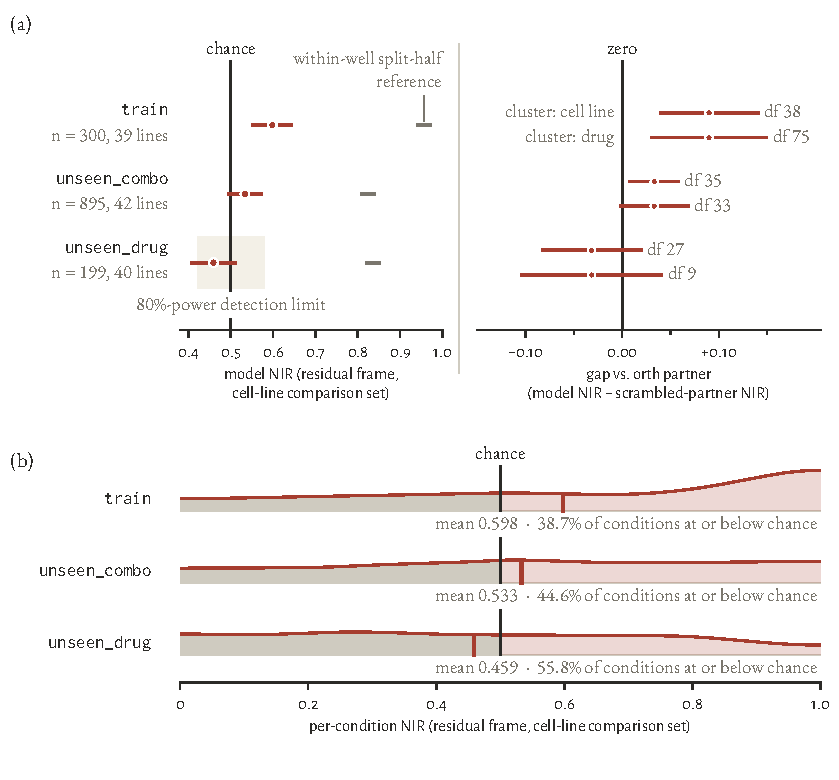
\includegraphics{fig-splits}
\caption[Chance-clearing on trained conditions only]{\captiontitle{The residual-frame
model clears chance on trained conditions only; the held-out-combination gap
excludes zero clustered on cell line but not clustered on drug, and the
unseen-drug gap flips sign.} Residual frame throughout, and $\NIR$ ranks each
prediction against the other drugs measured in the same cell line.
\textbf{(a)}~Left, model $\NIR$ against the chance value $0.5$ (solid rule), with
$95\%$ two-way cluster-robust intervals; $n = 300$, \needsaudit{895} and $199$ conditions on
\texttt{train}, \texttt{unseen\_combo} and \texttt{unseen\_drug}. The grey
dash on each row is that split's raw within-well split-half precision
reference, a measurement-precision figure computed from two halves of the same
well and not a replicate experiment; it carries no interval and is drawn as a
bare marker, and only \texttt{train} is filtered at the reliability line. Right,
on its own axis, the gap against the geometry-defined \texttt{orth} partner. Each
row has one point estimate, drawn twice with two intervals because the verdict
depends on which unit of generalisation is clustered: cell-line-clustered above,
drug-clustered below, each labelled with the Student~$t$ degrees of freedom it is
carried on. The grey band on the \texttt{unseen\_drug} row is that arm's
$80\%$-power detection limit around chance, $\pm 0.079$, the smallest departure
the arm could detect and not a confidence region. \textbf{(b)}~The per-condition
$\NIR$ distributions behind those three means, as reflected-boundary kernel
densities on a shared axis, each with its mean marked and the region at or below
chance shaded. The pooled $0.537$ is a mean over nearly flat distributions rather
than a location: even on \texttt{train}, $38.7\%$ of conditions sit at or below
chance, against $44.6\%$ and $55.8\%$ on the two held-out splits.}
\label{fig:splits}
\end{fullwidth}
\end{figure}


% FLAGGED, NOT FIXED -- the two panel-B numbers below (train $0.955$ and the
% spread $0.006$) are inherited from a superseded reconstruction taken at a
% +0.109 reliability line. This document defines the line at +0.1086: see :214
% ("$+0.109$, resolving to $+0.1086$"), :222-223 ("none falls at or below the
% resolved $+0.1086$") and :986 ("499 conditions sit below the $+0.1086$ line").
% Recomputed from RESULTS_cluster/re_v3.json -> records[] at repro_cos > 0.1086:
%   train         kept 300  0.9555006 -> 0.956   (:222-223 requires all 300)
%   unseen_combo  kept 396  0.9605642 -> 0.961   (:986's 499-below requires 396)
%   unseen_drug   kept 111  0.9597734 -> 0.960
%   spread: raw 0.0050636 -> 0.005, and max(rounded) - min(rounded)
%           = 0.961 - 0.956 = 0.005. BOTH conventions give 0.005 at the resolved
%           line, so this is NOT the convention clash it was reported as. 0.006
%           is just the old line's rounded-endpoint spread, 0.961 - 0.955. At
%           0.109 the kept counts are 299 / 394 / 111, which contradict :222-223
%           and :986 directly.
% The $0.132$ in the same sentence is unaffected: panel A is read straight from
% CANONICAL_NUMBERS.json -> ceilings{}, and raw (0.13178) and rounded-endpoint
% (0.956 - 0.824) both give 0.132 there.
% NOT CHANGED HERE because the correction is a six-site edit and four sites are
% outside this file: 05-Limitations.tex:224 and :225, 03-Apparatus.tex:378, and
% figs/splitref.tex's spread node (:219) and caption (:244). That figure already
% DRAWS train as 0.956 at the resolved line while the prose here still prints
% 0.955, so the disagreement is live. Changing this site alone would replace a
% uniformly wrong number with an inconsistent document. Reported upward instead.
The three splits are not scored on comparable populations either, and the
difference is one of selection. Their raw within-well split-half precision
references, the grey dashes of \cref{fig:splits}a, are $0.956$, $0.824$ and
$0.836$, a spread of $0.132$; \texttt{train}
is filtered at a reliability line the two held-out splits are not, and imposing
that line on all three brings the references to $0.955$, $0.961$ and $0.960$, a
spread of $0.006$. The held-out shortfall therefore cannot be softened by appeal
to a lower noise floor.

% PLACEMENT ONLY. The other retraction in this section is guarded at the
% \needspace above; this one was not, and it broke 13 lines / 2 lines across the
% page. The two lines that landed overleaf are the ones that perform the
% withdrawal, and they arrived with no CORRECTION rule above them, so the reader
% met the retraction as unlabelled prose. \budgettick reserves 5\baselineskip,
% which is not enough: the box measures 247.1pt, 16.6 lines with its padding and
% frame, so 17 is the box entire and it either sets whole here or starts the
% next page whole.
% MEASURED COST, build of 2026-08-12: the guard carries ~2.6 lines of the
% chapter forward. That stops the closing claim of \cref{sec:res-lookup}
% breaking, and starts the coverage definition and the seen-drug-transfer claim
% breaking, all three in 04d-baselines.tex, each of which wants the same guard.
\needspace{17\baselineskip}%

\paragraph{Regression recovers prompt sensitivity} 

Every condition $i$ contributes three scrambled prompts, one per stratum,
each naming a partner drug $p(i,s)$ whose true residual sits at a measured cosine
from the target's. Pooling all three prompts of every condition,
\begin{equation}
 \NIR_{i,s} \;=\; \alpha \;+\; \beta\,
   \cos\!\big(\resid_{p(i,s)},\, \resid_{i}\big) \;+\; \varepsilon_{i,s},
 \qquad s \in \{\texttt{near},\, \texttt{orth},\, \texttt{opposite}\},
\end{equation}
fitted by ordinary least squares with one intercept per condition, so that each
condition is compared only with itself and no part of the slope can come from
conditions differing from one another. The target-drug prompt is never a point on
this line --- only
the three scrambles are --- so nothing in the fit contrasts the model against a
chosen baseline, and $\beta$ is not a gap. It answers a different question: does
the score move with how similar the drug the model was \emph{told} is to the drug
the condition actually received? And $\beta = 0$ is the null by construction, since
a checkpoint that ignores the name emits the same distribution whichever partner
is substituted, putting its three points at one height whatever their cosines
happen to be. No comparator can be blamed for the answer, because none enters it.

Measured, $\beta$ is \ci{+0.361}{+0.249}{+0.472} on \texttt{train},
\ci{+0.321}{+0.207}{+0.434} on \texttt{unseen\_combo} and
\ci{+0.324}{+0.146}{+0.502} on \texttt{unseen\_drug}, clustered on the drug, and
all three still exclude zero clustered on the cell line ($[+0.240, +0.482]$,
$[+0.235, +0.406]$ and $[+0.234, +0.414]$), on $900$, $\num{2685}$ and $597$
points across $300$, $895$ and $199$ conditions. Pooling the conditions instead
of giving each its own intercept moves the estimates barely, to $+0.373$, $+0.336$
and $+0.342$, so unlike the arms of \cref{sec:res-blind} and
\cref{sec:res-epsilon} this one does not depend on the choice. The prediction tracks the drug it is named on every split,
held-out ones included. One restriction attaches to the last: on
\texttt{unseen\_drug} the partners named are overwhelmingly drugs the model
\emph{was} trained on, so the slope there shows it responding to a named trained
drug while scoring a condition whose own drug was withheld, and not that it knows
the withheld drug.


\paragraph{A positive slope beside a chance-level score is not a contradiction}
The two instruments conflict only if they ask the same question, and they do not.
The slope asks whether the prediction moves with the drug it is named. $\NIR$ asks
whether it lands nearer that condition's own truth than the truths of the
$\approx 40$ other drugs in the same cell line. A model passes the first and fails
the second by knowing what a drug does on average and not what it does
\emph{here}, and the size of that shortfall is itself measured:
\cref{sec:res-transfer} puts the share of a drug's residual that transfers across
contexts at \ci{\Tcoef = 0.553}{0.514}{0.593}, leaving
\ci{44.7\%}{40.7\%}{48.6\%} that does not, a remainder mixing cell line, dose,
well and estimator noise. The slope reads the transferable part; winning a ranking
needs the rest. It is also why the lookup wins in \cref{sec:res-lookup}, since
\texttt{drug\_lookup} is that same main effect, estimated straight from data far
more precisely than the model learned it. The condition-level picture agrees: on
trained conditions the cosine between prediction and own truth averages $+0.0389$
(sd $0.1119$, median $+0.0220$), spanning $[-0.3046, +0.3976]$ with $33.7\%$
clearing $|0.1|$ --- predictions pointing the right way on average, and seldom far
enough to win.

\paragraph{One asymmetry attaches to every held-out number in this chapter} The
evaluation's truths are not refitted. The generic is reconstructed from the
build's own fit inventory and verified against the build's \texttt{fit\_digest},
and a mismatch aborts the run. The reliability line selects the \emph{training}
split, so \texttt{train} is by construction the reliability-surviving population,
and the two held-out splits are not filtered at all. In the unseen-combination
arm $\num{499}$ conditions sit below the $+0.1086$ line and $\num{74}$ have a
negative split-half cosine; in the unseen-drug arm, of $\num{199}$ conditions,
$\num{88}$ sit below the line and $\num{18}$ are negative. This is deliberate,
since filtering the evaluation set on its own outcome is the selection this
chapter removed, but it leaves the comparison conservative in the direction that
matters. The held-out arms are scored on their full, noisier populations while
the trained arm is not.

% PLACEMENT ONLY. This box is 23 lines and it was breaking after two of them,
% which is the one split `breakable' is not for: the accent rule, the words "The
% claim." and two lines at the foot of the page, and the whole verdict overleaf.
% It fits on one page with room to spare, so the reservation is the whole box.
\needspace{24\baselineskip}%
\begin{claim}
  Re-encoding the target made the model respond to the combined drug-and-mechanism
  prompt. That much is established and survives every stress: on trained conditions
  it holds clustered on the cell line and on the drug, it holds against chance with
  no comparator at all, and the comparator-free slope excludes zero on all three
  splits under both clusterings --- \ci{+0.361}{+0.249}{+0.472},
  \ci{+0.321}{+0.207}{+0.434} and \ci{+0.324}{+0.146}{+0.502}, fitted with one
  intercept per condition so that each condition is compared only with itself.
  
  Transfer is a different question, and the two instruments answer it with very
  different confidence. The scramble intervention answers it barely. On
  \texttt{unseen\_combo} the gap is $+0.0332$, excluding zero clustered on cell line
  and well, \ci{+0.0332}{+0.0069}{+0.0594}, but not clustered on drug and well,
  \ci{+0.0332}{-0.0031}{+0.0695}, and it is the drug axis a drug-specific claim has
  to survive. The split is weaker than its name --- $30$ of its $34$ drugs and $39$
  of its $42$ cell lines appear in training, and $82\%$ of its conditions recombine
  a seen drug with a seen cell line --- and the effect is a majority tilt rather
  than a uniform one, positive for $20$ of $34$ drugs (sign test $p = 0.39$). The
  model's own $\NIR$ covers chance on both held-out splits. Transfer is
  \notestablished.
  
  The regression answers the same question far more confidently, and the distance
  between the two verdicts is itself the finding. Every point in it is a scrambled
  prompt, so it never asks whether the model is right, only whether it tells wrong
  answers apart --- and by that measure it tells them apart cleanly on every split,
  held-out ones included. Intervening directly on the prompt does not recover an
  effect of the same weight, perhaps because ranking a condition against its neighbours
  needs the part of the residual that does not transfer across contexts, which
  \cref{sec:res-transfer} measures at \ci{44.7\%}{40.7\%}{48.6\%}. 
  
  What the slope on the \emph{unseen-drug} split does and does not add has to be
  stated exactly. At \ci{+0.324}{+0.146}{+0.502} it shows that the prediction still
  tracks the drug \emph{named in the prompt} when the condition's own drug was held
  out. But the drugs named in that regression are the three scrambled partners,
  which on this split are overwhelmingly training drugs, and the real target-drug
  prompt contributes no point to it. The slope is evidence that the model responds
  to named trained drugs in an unseen-drug scoring context, and not evidence that it
  knows the held-out drugs.
  \end{claim}
% 04d-baselines.tex -- beats 7-9 and the ledger. sec:res-field has NO claim
% block, deliberately. Source: Investigation-v4.tex 2392-2938. Numbers verbatim
% from v1; two pending-audit flags. "the bar" = training-only drug_lookup;
% "the reference" = within-well split-half; "the threshold" = 0.80.

\beatsection{R}{7}{A lookup table wins}{sec:res-lookup}
\label{sec:methods-baselines}

\begin{question}[7]
What does a drug-response prediction have to beat before it is worth having? The
instrument is a ladder of predictors scored through one pipeline, the lowest rung
of which needs no model at all, only a table of what each drug did elsewhere.
That table wins.
\end{question}

\noindent
Every section so far has asked whether the model uses the drug at all --- whether
the token is read, whether the prediction moves when it moves, whether any of that
survives a holdout. Those are questions about mechanism, and they set the lowest
bar that a model that claims to make predictions based on context must clear. This section changes the question to what the prediction is worth,
which is not a question about the model alone but a comparison against what can be
had without one. A model can respond to the drug in its prompt and still predict
badly, so the pre-registered bar was never ``beats chance''. Residual targets are
plausibly memorisable, and a predictor that looks up what this drug did elsewhere
needs no checkpoint at all.\gloss{lookup}{Predicts this drug's residual as its mean
residual in the \emph{other} cell lines.} 
% --------------------------------------------------------------------------

% ---------------------------------------------------------------------------
\paragraph{What the ladder is, and what keeps it fair} Every arm in
\cref{tab:lookup} predicts the same object --- a condition's drug-specific
residual --- and is scored through one pipeline, on the same truths, the same
encoding and the same comparison set, so that the only thing separating the rungs
is what each is allowed to know. Scores are $\NIR$ in the \Rframe{} frame, where
chance is $0.50$; \cref{fig:ladder} draws the same numbers against chance
and the reference.

The rungs run from most informed to least. At the top sits the within-well
split-half reference, which is not a predictor at all but a precision ceiling: a
disjoint half of the same well's cells substituted for the prediction, scoring
$0.854$. Below it come two lookups that use no model, no prompt and no checkpoint.
\texttt{drug\_lookup} predicts a condition's residual as that drug's mean residual
across \emph{all} the other cell lines it was run in. \texttt{drug\_lookup\_1}
narrows that to one other cell line, chosen at random: it still averages the
drug's conditions \emph{within} that line, which are usually several doses, but it
never averages across lines. The pair exists to separate memorising a drug from
being denoised by repetition, since \texttt{drug\_lookup} is an average over many
lines while the reference it is read against is one noisy half of a well against
another. \texttt{moa\_lookup} drops
from the drug to its class, predicting from other drugs that share this drug's
mechanism annotation. The model sits below these, given a control cell and the
drug. Beneath it are three arms that know nothing about the drug at all and fix
the floor: \texttt{control\_copy} returns the untreated cell unchanged,
\texttt{generic} predicts the average response, which in this frame is the zero
vector, and \texttt{random} is what its name says.

Three supports are in play, and rows may not be read across them. The reference,
the model and the drug-agnostic arms are scored on all $\num{1394}$ conditions.
A drug lookup is undefined wherever a drug has no
\emph{training} condition in a cell line other than the one being scored, which
drops the $\num{199}$ unseen-drug conditions, whose drug was withheld from
fine-tuning altogether, together with three whose only training conditions sit in
the cell line under test. That leaves the lookups a common support of
$\num{1192}$, on which the model and the reference score $0.549$ and $0.857$
rather than the $0.537$ and $0.854$ they score on the full set.
\texttt{moa\_lookup} is narrower again at $\num{218}$. Even
the reference moves between the first two, which is why a mark in one column of
\cref{fig:ladder} may not be set beside a mark in another.

Two disciplines keep the lookups from becoming oracles. They are fitted from
training conditions only: fitted from the full cache, a lookup scoring a held-out
condition would read residuals the model was never shown, an oracle and not a
baseline, so that construction is excluded. And \texttt{drug\_lookup\_1}, having
picked its one cell line, averages that line's conditions rather than drawing a
single condition from it, because $62\%$ of drugs are multi-dose and one condition
would confound ``different cell line'' with ``different dose''. \texttt{moa\_lookup} is not an oracle in any split either: its
partner pool is restricted to \emph{training} conditions in the same cell line, so
a held-out condition never enters the prediction made for it.

\begin{defn}{Coverage of the reference}
A predictor's \emph{coverage} is the fraction of the distance from chance to the
within-well split-half precision reference that it closes,
\[
  (\NIR_{\text{arm}} - 0.50)\,/\,(\NIR_{\text{ref}} - 0.50).
\]
Coverage above $100\%$ therefore means the arm scores above the reference, a
statement about the reference and not a headroom estimate. Reference and coverage
are computed on the same support as the arm they describe.
\end{defn}

% ---------------------------------------------------------------------------
\begin{figure}[htbp]
% NOT \begin{fullwidth}. Laid out at the 142mm body block, which returns this
% page's margin notes: the MoA column carries two marks in the bottom sixth and
% the upper two-thirds of a 174mm strip would be blank, so the width is not
% earned. Body only; the tikzpicture lives in figs/ladder.tex, and every number
% it draws is listed with its source pointer in figs/fig-ladder.json.
\centering
% ===========================================================================
% figs/ladder.tex -- fig:ladder, reworked for thesis_v2.
% FIGURE BODY ONLY. No preamble, no document environment. \input it from
% inside a plain figure float (NOT fullwidth) in Sections/04d-baselines.tex.
%
% This is the SUPPORT figure: three columns at three different supports
% (n = 1394 / 1192 / 218), each showing where its arms sit between chance and
% the within-well split-half precision reference. It is deliberately distinct
% from fig:two-scales, which is the FRAME figure. The argument is unchanged.
%
% WHAT CHANGED FROM THE INLINE v2 VERSION (five spec'd fixes, plus one number
% correction that is NOT cosmetic -- see PROVENANCE note 3 below):
%
%   (1) The chance rule at 0.50 struck through the word "generic", whose label
%       sat at its own value of exactly 0.500. The caption states that labels a
%       rule would strike are lifted clear; "generic" had slipped through it.
%       Its label is now lifted BELOW the rule (0.500 -> 0.478) with a leader.
%   (2) The 115.7% brace and its label sat hard against the col-1/col-2
%       divider. The brace stem is now at x=6.60, which is 2.15cm (61pt) clear
%       of the divider at x=4.45, and its label's left edge is 0.98cm (28pt)
%       clear of it. The tightest thing to the divider is now the 13.9% label,
%       whose left edge is 0.475cm (13.5pt) clear -- the spec asked for >=6pt
%       and every part of the brace apparatus beats that. The braces are NESTED,
%       short 13.9% brace outboard at x=5.95, tall 115.7% brace inboard at
%       x=6.60, with each label at its own brace's height. That is the only
%       nesting in which neither label crosses the other's stem: the short
%       brace exists only over y in [0.500,0.549], so the tall brace's label,
%       sitting at y=0.71, has nothing in its way.
%   (3) The four left-column leaders all left the same 3-dot blob at
%       0.506/0.501/0.500 (0.8mm and 0.16mm apart on this scale, against a
%       1.0mm dot). control_copy / random / generic are now dodged sideways to
%       x = 0.30 / 0.58 / 0.86 so each leader leaves its own dot, and the four
%       label heights (0.645 / 0.583 / 0.532 / 0.478) fan the leaders to four
%       clearly different angles. Horizontal position inside a column carries
%       no meaning; the caption says so.
%   (4) \begin{fullwidth} DROPPED. Laid out at 142mm (the v2 body block), which
%       returns that page's margin notes. Drawn extent is 13.96cm of 14.20cm
%       (measured: 400.4pt of the 404.03pt block). Nothing is \resizebox'd:
%       1cm here is 1cm on the page, and 9pt type prints at 9pt.
%   (5) Label typography reduced from four registers to three, and the key is
%       stated in the caption:
%             \ttfamily ink      an arm, named as tab:lookup names it
%             roman     ink      prose ("within-well reference")
%             roman     accent   the model
%       v1/inline-v2 set "model" in \textbf + accent, a fourth register with no
%       key, and split the identifiers arbitrarily between ink and quietink.
%       quietink is now furniture only (ticks, support sizes, axis name).
%   Also, neither spec'd nor argument-bearing:
%     - the y axis had no name. It now carries one (NIR, RESID frame), set at
%       the top of the tick column so it costs the figure no width;
%     - gridlines are broken at the dividers. The caption forbids reading
%       across columns and an unbroken full-width rule invites exactly that;
%     - every dot gets a white halo, so the two arms that sit ON the chance
%       rule (random 0.501, generic 0.500) read as marks rather than as
%       thickenings of the rule. Same device as the interrupted zero rule in
%       figs/comparators.tex.
%
% PROVENANCE of every number drawn is in fig-ladder.json, sibling to this file.
% Source for all of it: RESULTS_cluster/re_v3.json.
%   1. Column 1 (n=1394) reads means/{ceiling,model,control_copy,random,generic}.
%   2. Column 2 (n=1192) reads means/common_support/{model,ceiling,drug_lookup}
%      and means/drug_lookup_1, and the two coverage figures read
%      means/common_support/{coverage_model,coverage_lookup}.
%   3. Column 3 (n=218). moa_lookup = means/moa_lookup = 0.5520. The model mark
%      in this column was 0.549 -- that is the model's COMMON-SUPPORT value
%      reused on a different support, and it is wrong. The model's mean over
%      the 218 MoA-support conditions is 0.5956 (mean of records[].model over
%      the 218 records that carry a moa_lookup value). Check: 0.595575 minus
%      0.552015 = 0.043560, which reproduces means/vs_baselines/moa_lookup/gap
%      = 0.0435594 to six decimals -- the same +0.0436 the tab:lookup caption
%      quotes. At 0.549 the figure put the model BELOW moa_lookup, the wrong
%      sign for a gap the text states as positive. The mark is drawn at 0.596.
%      No claim moves: the two-way interval [-0.0480,+0.1352] still spans zero,
%      so moa_lookup is still "not separated from the model".
% ===========================================================================
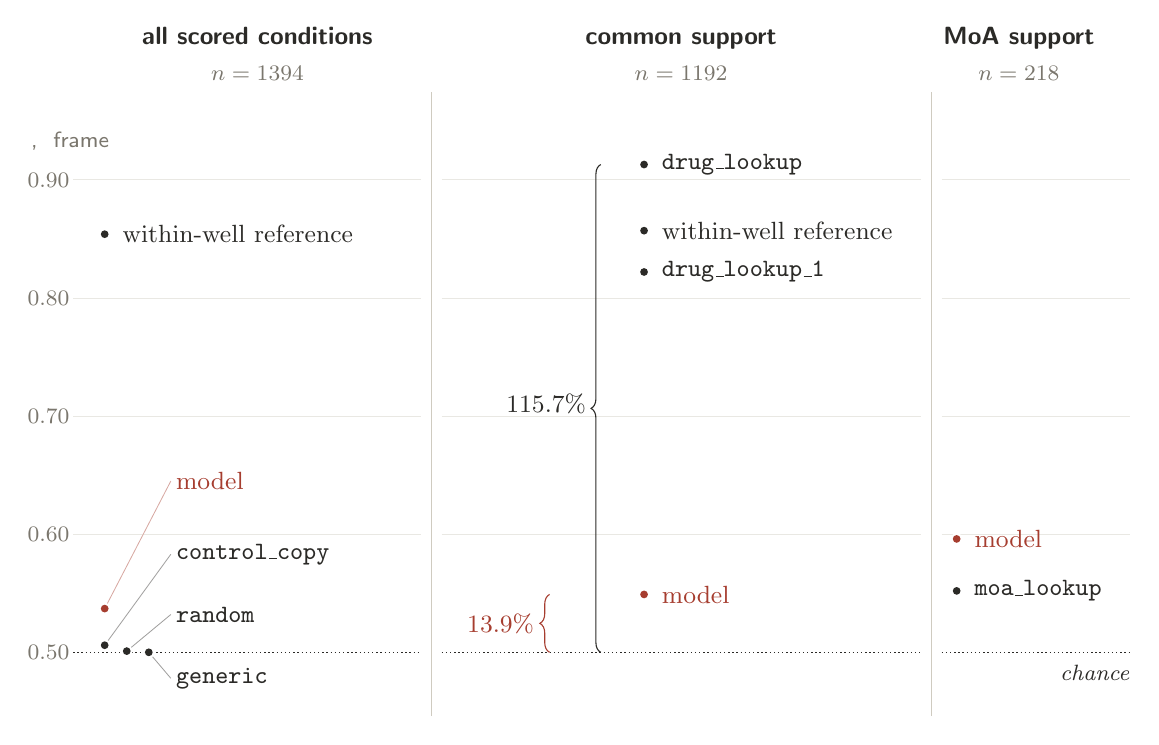
\begin{tikzpicture}[x=1cm, y=72mm, every node/.style={inner sep=0pt}]

  % --- value-to-position map. One map, one axis, all three columns. ---------
  \def\lo{0.47}\def\hi{0.95}
  \def\Y#1{{(#1-\lo)/(\hi-\lo)}}

  % --- the three registers of label type, and the furniture sizes. ---------
  % 9pt, not \scriptsize (8pt): this figure is drawn at its final size and is
  % never scaled, so its type may sit just under the 11pt caption rather than
  % being shrunk below it.
  \def\marklab{\fontsize{9}{10.5}\selectfont}
  \def\ticklab{\fontsize{8}{9}\selectfont}
  \def\headlab{\sffamily\fontsize{9}{10.5}\selectfont\bfseries}
  \def\subhead{\sffamily\fontsize{8}{9.5}\selectfont}

  % --- column geometry (cm): the two dividers and the right edge. ----------
  \def\Da{4.45}\def\Db{10.80}\def\R{13.32}

  % --- drawing macros. Order of use is leaders, then dots, then labels, so a
  %     dot and its halo always cover the tail of its own leader. -----------
  \newcommand{\lead}[5]{\draw[#5!45, line width=0.3pt]
     (#1,\Y{#2}) -- (#3-0.06,\Y{#4});}
  \newcommand{\dotat}[3]{\fill[white] (#1,\Y{#2}) circle (2.1pt);
     \fill[#3] (#1,\Y{#2}) circle (1.4pt);}
  \newcommand{\labat}[4]{\node[anchor=west, text=#3, font=\marklab]
     at (#1,\Y{#2}) {#4};}

  % --- gridlines, broken at the dividers ------------------------------------
  \foreach \v in {0.60,0.70,0.80,0.90}{
    \draw[rulegrey!45, line width=0.3pt] (-0.10,\Y{\v}) -- (4.32,\Y{\v});
    \draw[rulegrey!45, line width=0.3pt] ( 4.58,\Y{\v}) -- (10.67,\Y{\v});
    \draw[rulegrey!45, line width=0.3pt] (10.93,\Y{\v}) -- (\R,\Y{\v});}
  \foreach \v in {0.50,0.60,0.70,0.80,0.90}{
    \node[anchor=east, font=\ticklab, text=quietink] at (-0.14,\Y{\v}) {\v};}

  % --- the chance rule. Drawn, and named, because the axis is NIR. ----------
  \draw[ink, line width=0.5pt, densely dotted] (-0.10,\Y{0.50}) -- (4.32,\Y{0.50});
  \draw[ink, line width=0.5pt, densely dotted] ( 4.58,\Y{0.50}) -- (10.67,\Y{0.50});
  \draw[ink, line width=0.5pt, densely dotted] (10.93,\Y{0.50}) -- (\R,\Y{0.50});
  \node[anchor=east, font=\ticklab\itshape, text=ink] at (\R,\Y{0.483}) {chance};

  % --- what the axis is -----------------------------------------------------
  \node[anchor=west, font=\subhead, text=quietink]
    at (-0.64,\Y{0.933}) {$\NIR$, \Rframe{} frame};

  % --- column dividers and column heads -------------------------------------
  \draw[rulegrey, line width=0.4pt] (\Da,-0.05) -- (\Da,1.05);
  \draw[rulegrey, line width=0.4pt] (\Db,-0.05) -- (\Db,1.05);
  \node[anchor=south, align=center, text=ink] at (2.24,1.07)
    {{\headlab all scored conditions}\\[0.2ex]{\subhead\color{quietink}$n = \num{1394}$}};
  \node[anchor=south, align=center, text=ink] at (7.62,1.07)
    {{\headlab common support}\\[0.2ex]{\subhead\color{quietink}$n = \num{1192}$}};
  \node[anchor=south, align=center, text=ink] at (11.91,1.07)
    {{\headlab MoA support}\\[0.2ex]{\subhead\color{quietink}$n = \num{218}$}};

  % =========================================================================
  % COLUMN 1 -- all scored conditions, n = 1394
  % =========================================================================
  % Four fanned leaders. Dots are dodged sideways only where values coincide:
  % control_copy 0.506, random 0.501, generic 0.500 are 0.8mm and 0.16mm apart
  % vertically here, against a 1.0mm dot.
  \lead{0.30}{0.537}{1.20}{0.645}{accent}
  \lead{0.30}{0.506}{1.20}{0.583}{ink}
  \lead{0.58}{0.501}{1.20}{0.532}{ink}
  \lead{0.86}{0.500}{1.20}{0.478}{ink}

  \dotat{0.30}{0.854}{ink}
  \dotat{0.30}{0.537}{accent}
  \dotat{0.30}{0.506}{ink}
  \dotat{0.58}{0.501}{ink}
  \dotat{0.86}{0.500}{ink}

  \labat{0.52}{0.854}{ink}{within-well reference}
  \labat{1.20}{0.645}{accent}{model}
  \labat{1.20}{0.583}{ink}{\ttfamily control\_copy}
  \labat{1.20}{0.532}{ink}{\ttfamily random}
  \labat{1.20}{0.478}{ink}{\ttfamily generic}

  % =========================================================================
  % COLUMN 2 -- common support of the drug lookups, n = 1192
  % =========================================================================
  % Coverage of the reference, (arm - 0.50) / (reference - 0.50), both on THIS
  % support. Braces first so the dots' halos are not cut by a brace stem.
  \draw[decorate, decoration={brace, amplitude=3.5pt}, accent, line width=0.4pt]
    (5.95,\Y{0.500}) -- (5.95,\Y{0.549});
  \node[anchor=east, font=\marklab, text=accent] at (5.76,\Y{0.5245}) {$13.9\%$};
  \draw[decorate, decoration={brace, amplitude=3.5pt}, ink, line width=0.4pt]
    (6.60,\Y{0.500}) -- (6.60,\Y{0.913});
  \node[anchor=east, font=\marklab, text=ink] at (6.42,\Y{0.710}) {$115.7\%$};

  \dotat{7.15}{0.913}{ink}
  \dotat{7.15}{0.857}{ink}
  \dotat{7.15}{0.822}{ink}
  \dotat{7.15}{0.549}{accent}

  \labat{7.37}{0.913}{ink}{\ttfamily drug\_lookup}
  \labat{7.37}{0.857}{ink}{within-well reference}
  \labat{7.37}{0.822}{ink}{\ttfamily drug\_lookup\_1}
  \labat{7.37}{0.549}{accent}{model}

  % =========================================================================
  % COLUMN 3 -- conditions with an MoA partner pool, n = 218
  % =========================================================================
  \dotat{11.12}{0.596}{accent}
  \dotat{11.12}{0.552}{ink}

  \labat{11.34}{0.596}{accent}{model}
  \labat{11.34}{0.552}{ink}{\ttfamily moa\_lookup}

\end{tikzpicture}

\caption[The baseline ladder]{\captiontitle{A predictor that needs no model, no prompt
and no checkpoint scores above the reference the model is measured against, and
the three columns may not be read across.} Marks are $\NIR$ in the \Rframe{}
frame, where chance is $0.50$. Each column is scored on its own support
($n = \num{1394}$, $\num{1192}$ and $\num{218}$), so a mark in one may not be set
beside a mark in another; even the reference differs between the first two. On
the common support the model covers $13.9\%$ of the distance from chance to the
within-well split-half precision reference, and a training-only per-drug lookup
covers $115.7\%$ of it, which is a property of the reference and not headroom
(\cref{tab:lookup}). On the MoA support the model scores $0.596$ against
\texttt{moa\_lookup}'s $0.552$, a $+0.0436$ the interval does not separate from
zero. No interval is drawn: the source gives them on differences between arms,
not on the level of one arm, and those are in \cref{tab:lookup}. \emph{Reading
the labels}: monospace names an arm exactly as \cref{tab:lookup} names it, roman
names the reference in prose, the accent marks the model, and there is no fourth
style. A label a rule would strike or a neighbour would crowd is lifted clear on
a hairline; the dot carries the value. Horizontal position inside a column means
nothing, and arms whose scores nearly coincide are dodged sideways so each keeps
its own dot.}
\label{fig:ladder}
\end{figure}

% ---------------------------------------------------------------------------
\begin{table}[htbp]
% MARGINALIA: in-column ladder. The full caption stays ABOVE at text width:
% the spec's trim would have dropped the moa_lookup interval and the
% "must not be compared" clause, which the body does not repeat. The Note
% column and the general note go to the margin beside the table.
\caption{\captiontitle{A training-only per-drug lookup is the bar to beat.} Reference,
model and drug-agnostic arms use all $\num{1394}$ conditions; the drug lookups
exist on a common support of $\num{1192}$, where model and reference score
$0.549$ and $0.857$. There, model minus \texttt{drug\_lookup} is
\ci{-0.3631}{-0.3982}{-0.3280}; the lookup scores $0.913$ pooled, $0.980$ on
trained conditions and $0.890$ on held-out wells, where its same-well advantage
is absent. \texttt{moa\_lookup} has narrower support ($n = \num{218}$) and is not
separated from the model (\ci{+0.0436}{-0.0480}{+0.1352}); its pooled row must
not be compared with rows on other supports. The bar is each arm's distance above
chance ($0.50$) on a common axis to $1.0$.}
\label{tab:lookup}
\begin{lrbox}{\tvfb}
\begin{tabularx}{\textwidth}{@{}L{36mm} Y r l@{}}
\thead{Arm} & \thead{What it knows} & \multicolumn{1}{r}{\thead{$\NIR$}} & \thead{Above chance}\\
\midrule
\quiet{within-well split-half reference} & \quiet{disjoint cell halves, one well} & 0.854 & \nirbar[quietink]{0.854}\\
\addlinespace[10pt]
\arm{drug_lookup} (training-only) & drug's mean residual, other lines & \key{0.913} & \nirbar{0.913}\\
\arm{drug_lookup_1} & the same, from one other cell line & 0.822 & \nirbar{0.822}\\
\arm{moa_lookup} ($n = \num{218}$) & drugs sharing this drug's MoA & 0.552 & \nirbar{0.552}\\
\addlinespace[10pt]
\textbf{model} & control cell $+$ drug & 0.537 & \nirbar{0.537}\\
\addlinespace[10pt]
\arm{control_copy} & nothing (copies the control) & 0.506 & \nirbar{0.506}\\
\arm{generic} & nothing (predicts the average) & 0.500 & \nirbar{0.500}\\
\arm{random} & nothing & 0.501 & \nirbar{0.501}\\
\end{tabularx}
\end{lrbox}
\tablemarginnotes{%
  \rownote{reference}{precision, not a replicate; $0.857$ on the lookups' support}
  \rownote{drug_lookup}{the bar to beat; $n = \num{1192}$}
  \rownote{drug_lookup_1}{still beats the model; same support}
  \rownote{moa_lookup}{narrower support; not separated}
  \rownote{model}{$0.549$ on the lookups' $n = \num{1192}$}
  \rownote{control_copy}{drug-agnostic}
  \rownote{generic}{the zero vector}
  \rownote{random}{floor}
  \par\addvspace{6pt}Rows on different supports are not comparable. Chance is $0.50$ in the
  \Rframe{} frame under the exchangeability condition audited in \cref{sec:res-metrics}.}
\end{table}

% ---------------------------------------------------------------------------
\paragraph{Above chance, and below the table} The outcome predicted before the
comparison was run was that the model would land above chance and below the
lookup, and that is where it lands. On the $\num{1192}$ conditions where both are
defined it scores $0.549$, above the $0.50$ chance line and well below
\texttt{drug\_lookup}'s $0.913$; the difference is
\ci{-0.3631}{-0.3982}{-0.3280}. What that licenses was fixed in advance and is
narrow: the model recovers something of a drug's average residual and adds no
tailoring to the cell line in front of it, since a table holding that average
already beats it. Transfer to held-out combinations is \notestablished
(\cref{sec:res-generalisation}). 

\paragraph{This is DrEval's finding, in transcriptomic space} The finding travels
furthest of anything here, needing no checkpoint, no prompt and no cell-sentence
encoding. DrEval reports that deep learning models barely outperform a naive
predictor of mean drug and cell-line effects~\cite{dreval}, and our
\texttt{drug\_lookup} is
the $\beta(d)$ term of that additive model, measured where the
$\textrm{generic}(c)$ term has already been
subtracted.\seealso{\cref{sec:res-transfer} measures what that constant leaves
out} On a $946$-gene transcriptomic response, not a scalar potency, that drug
main effect reaches $0.913$, above the $0.857$ reference itself. DrEval's
inherited warning~\cite{partin}, that good pair-holdout performance is reachable
by predicting each drug's training average, is here the hypothesis. It holds.

\paragraph{The missing head-to-head, and why the bar survives it} A third
objection is that this chapter's model is the wrong one. A conditional model
built for perturbation response~\cite{cpa,scgen,gears} was never run on this
split, so the head-to-head a reader wants is missing, and that is a real gap. But
the ladder is architecture-free, so a competitor can be dropped in and scored,
and what it has to clear for a seen drug in a new context is
\texttt{drug\_lookup}, $0.913$ pooled, or $0.890$ on the held-out split. Not
$0.500$. For an unseen drug no lookup exists, so that regime needs a different
bar and gets one in \cref{sec:res-scope}.

\begin{scopelimit}[carried into \cref{sec:res-scope} and \cref{sec:limitations}]
The two regimes must not share a number. \texttt{drug\_lookup} is the bar for a
\emph{seen} drug in a new context. No lookup exists for a drug that never
appeared in training, so nothing here sets a bar for that regime. Neither may
rows on different supports be combined: $\num{1394}$, $\num{1192}$ and
$\num{218}$ select conditions by different rules, and a distance to the reference
is comparable within a support and not between supports.
\end{scopelimit}

\paragraph{Why the lookup beating the reference is not headroom} On the common
support the lookup scores \emph{above} the reference,
$\texttt{drug\_lookup} - \textrm{reference} = +0.056$, tempting to read as ``the
modelling target has vanished''. Three reasons, all favouring the lookup, block
that inference. The reference is scored against a half-sample truth and every
baseline against the full-sample truth; \texttt{drug\_lookup} averages
$\approx 38$ conditions against that single noisy half; and $\NIR$ near $0.91$
compresses most of the cosine range into a few thousandths. The coverage figures
are themselves distances to a split-half reference \cref{sec:methods-data} calls
optimistic; that optimism sits in the denominator and if anything makes both
coverage figures too small, while the half-sample truth of the first reason
pushes the other way. The net magnitude is unknown and the ordering carries the
claim.

\paragraph{Averaging is not why the lookup beats the model} Of those three
reasons only the averaging could also deflate the comparison with the model, and
\texttt{drug\_lookup\_1} tests it by drawing on one other cell line. It scores
$0.822$, and paired on the same support the model trails it by
\ci{-0.2723}{-0.3074}{-0.2372}, clustered two-way on cell line and well. This
drug's mean residual in one other cell line beats a $1$B-parameter model handed
this condition's own control cells. Neither gap is an average over a mixed
population (\cref{fig:paired-lookup}): condition by condition, the model scores
above \texttt{drug\_lookup} on $85$ of the $\num{1192}$ and above
\texttt{drug\_lookup\_1} on $214$, $7.1\%$ and $18.0\%$, counts over conditions
carrying no interval.

\paragraph{The bar is not equally clean on both sides of the split} The pooled
$0.913$ covers two populations. On trained conditions the lookup scores $0.980$.
On held-out wells, where it cannot borrow the target's own well, it scores
$0.890$ against the model's $0.533$ on the 893 held-out-well
conditions where both are scored, a count this thesis quotes two ways and has
under audit; the paired gap there is \ci{-0.357}{-0.403}{-0.311}. Nothing in the
argument turns on the exact size of that population. The ordering holds on both
sides, and the held-out side, where the well advantage is absent, is the side a
claim about transfer has to survive.

% ---------------------------------------------------------------------------
% \begin{fullwidth}: two square scatters side by side, each with its own
% difference histogram beneath, is a 174mm object -- squeezed to the 142mm body
% block the two panels lose the aspect that makes the identity line readable as
% a diagonal. Drawn at 174mm by thesis_v2/figs/paired-lookup.py, so NO width=
% key: it is placed at scale 1.0 and its type prints at the size it was set in.
% Every number it draws is listed with its source pointer in
% figs/fig-paired-lookup.json.
\begin{figure}[htbp]
\begin{fullwidth}
\raggedright
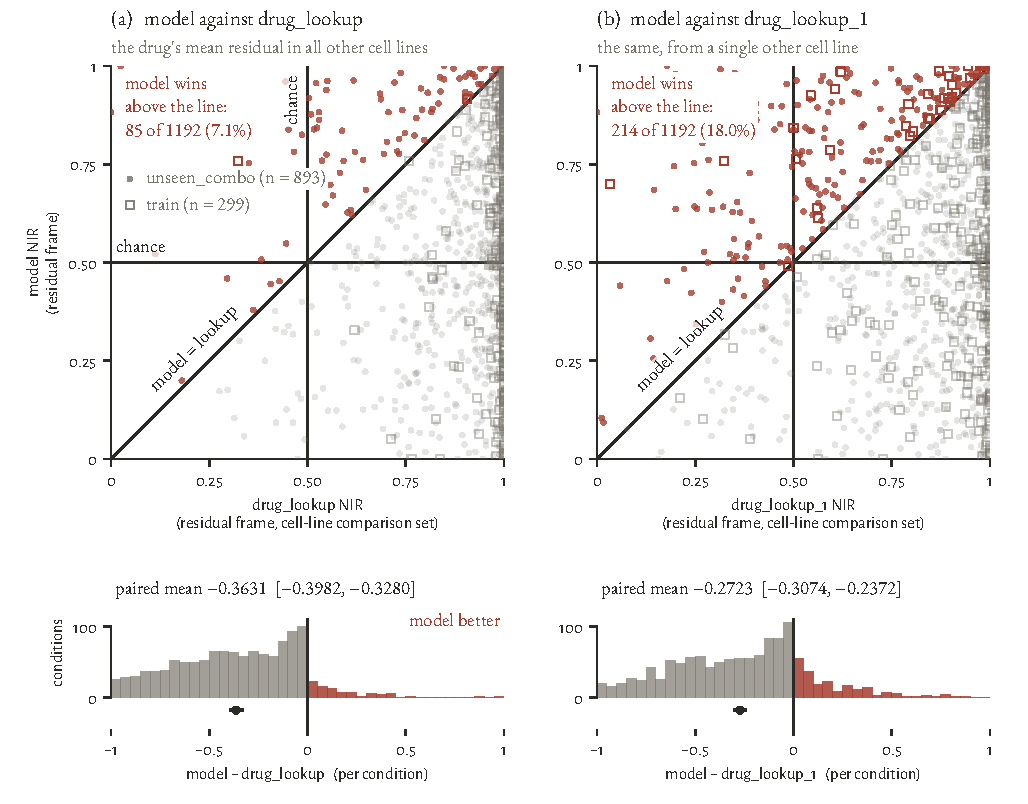
\includegraphics{fig-paired-lookup}
\caption[The model beats the lookup on 7.1\% of conditions]{\captiontitle{The headline
gap is a tilt of nearly the whole population and not a mean over a mixed one:
the model scores above \texttt{drug\_lookup} on $7.1\%$ of conditions, and above
the single-cell-line lookup on $18.0\%$.} Every mark is one of the $\num{1192}$
conditions of the common support --- those on which a training-only lookup
exists --- and both axes are $\NIR$ in the \Rframe{} frame, comparison set other
drugs in the same cell line. On this support the model scores $0.549$ and the
within-well split-half precision reference $0.857$; the $\num{1394}$-condition
figures quoted elsewhere ($0.537$ and $0.854$) are a different population and
are not combined with these. \textbf{(a)}~Against \texttt{drug\_lookup}, the
drug's mean residual in all other cell lines, $0.913$ pooled: the model is above
the identity line on $85$ of $\num{1192}$ conditions, $7.1\%$.
\textbf{(b)}~Against \texttt{drug\_lookup\_1}, the same quantity from a single
other cell line, $0.822$ pooled: $214$ of $\num{1192}$, $18.0\%$. Marker shape
gives the split, $\num{299}$ \texttt{train} and \needsaudit{893}
\texttt{unseen\_combo}; no \texttt{unseen\_drug} condition appears, because no
training lookup exists for a drug held out of training, and that regime is
therefore not addressed by this figure at all. The lower panels are the
per-condition paired difference on a shared count axis, with the paired mean
drawn below the counts as a point and bar, the bar a $95\%$ bootstrap interval
clustered two-way on cell line and well: \ci{-0.3631}{-0.3982}{-0.3280} in (a)
and \ci{-0.2723}{-0.3074}{-0.2372} in (b). The win counts are counts over
conditions and carry no interval; ties ($23$ and $28$ conditions) count as not a
win. The $0.50$ rules are chance on both axes, labelled once in (a).}
\label{fig:paired-lookup}
\end{fullwidth}
\end{figure}

\clearpage
% ===========================================================================
\beatsection{R}{8}{Same-target retrieval is the strongest observed lead}{sec:res-scope}

\begin{question}[8]
The bar just set exists only for a drug that appeared in training. A drug that
never did can be reached at all only through some property it shares with drugs
that were seen, a protein target, a mechanism, a chemical shape. The instrument
predicts each drug from its annotated neighbours in the same cell line, against a
null matched on everything but the channel itself. One channel carries a lead, on
a very short roster of drugs.
\end{question}

\noindent
The bar set in \cref{sec:res-lookup} exists only for a drug the model has already
met. \texttt{drug\_lookup} predicts a condition from that same drug's residual
measured in other cell lines, so it is undefined the moment the drug is new ---
which is the case a model would be worth having for in the first place. This
section asks what can replace it there: with a drug's own history unavailable, can
the drug be reached through the drugs it resembles?

Resemblance has to be defined along something, and that something is called a
\emph{channel} here. Tahoe's metadata annotates each drug several ways --- the
protein it targets, its mechanism class, its chemical structure --- and each
annotation induces a different set of neighbours. For a channel $X$, a drug's
residual is predicted as the mean residual of the other drugs in the same cell
line that share property $X$ with it, the construction of \texttt{moa\_lookup}
(\cref{sec:res-lookup}) generalised from mechanism to any annotated property. A
channel along which the response really varies should predict better than one
built from arbitrary neighbours; a channel carrying nothing should not.

\paragraph{The null, and what it has to hold fixed} That comparison is the entire
measurement, so the control decides what it is worth. Each channel arm is paired
with a \emph{plate-matched random null}: partners drawn from the same cell line,
in the same number, with the same split between the target's own plate and other
plates, but chosen at random instead of by the annotation. The matching is not
decoration. Drugs sharing a mechanism or a protein target are co-plated more often
than chance, so a null matched on partner count alone would differ from its arm in
plate membership as well as in the annotation --- two differences where the
estimand allows one, and the gap would then be reporting batch structure as
channel information. A second, count-matched null is reported alongside it as a
sensitivity check, and it is the weaker control precisely because it leaves that
second difference standing. Where a plate-matched null cannot be built across
enough cell lines the channel is reported \textsc{untestable} rather than closed,
because not being able to construct a control is not a negative result. Coverage
is read before any gap for the same reason: a channel annotated on a handful of
drugs was never really tested, and a null on it closes nothing.

% ---------------------------------------------------------------------------
\begin{table}[htbp]
% MARGINALIA: full width (six columns on one line need ~176mm). Caption above at
% the text width, notes below in the sans. One highlight: the one channel whose
% plate-matched lower bound clears the gate -- the same cell is keyed in the
% repeated Panel A of \cref{tab:fieldattribution}.
\caption{\captiontitle{Coverage first, then the gap.} The drugs behind each channel are
stated before any verdict, because a null result on a channel never really tested
is not a closure. The plate-matched null is the estimand-correct control; the
count-matched column shows sensitivity to plate membership, not a causal share.
The gate asks the plate-matched lower bound to clear a pre-set margin of $0.03$
clustered on cell line and well. On that axis, and only there, protein target
clears it ($+0.0745$) while mechanism ($+0.0279$) and chemistry ($+0.0035$) do
not. All three exclude zero, so the two that fail are inconclusive rather than
equivalent to their nulls, and neither may be written as closed.}
\label{tab:channels}
\begin{fullwidth}
\begin{threeparttable}
\begin{tabularx}{\linewidth}{@{}l r r l r Y@{}}
\thead{Channel} & \thead{Drugs (annot./scored)} & \thead{$n$}
  & \thead{vs plate-matched null} & \thead{(vs count-matched)}
  & \thead{Verdict} \\
\midrule
\key{protein target} & 264 / 18 & 712 & \ci{+0.1351}{+0.0745}{+0.1958}
  & $+0.1498$ & live, cell-line axis\tnote{$\dagger$} \\
mechanism (MoA) & 180 / 26 & 921 & \ci{+0.0805}{+0.0279}{+0.1332}
  & $+0.0623$ & inconclusive \\
chemical structure & 377 / 94 & \num{4131}
  & \ci{+0.0261}{+0.0035}{+0.0487} & $+0.0122$ & inconclusive \\
\end{tabularx}
\begin{tablenotes}
\item[$\dagger$] The axis is written into the target verdict because ``live'' is
not usable without it. Clustered on the drug, the target interval falls short of
this margin against both estimand-correct nulls and clears it only against the
weaker count-matched one.
\item The counts are annotations in Tahoe's drug metadata and not testable
coverage here; within this cache only $18$, $26$ and $94$ of the $94$ scored
drugs received a channel arm at all.
\end{tablenotes}
\end{threeparttable}
\end{fullwidth}
\end{table}

% ---------------------------------------------------------------------------
% \input, not \includegraphics: figs/gate.tex is TikZ and carries its own float,
% fullwidth block, caption and \label{fig:gate}. Its twelve intervals are
% literals transcribed from RESULTS_cluster/ and listed again, to machine
% precision and with their n, cluster keys, df and source paths, in the sibling
% figs/fig-gate.json.
% ===========================================================================
% gate.tex -- the channel gate, twelve intervals in three blocks.
% \input by Sections/04d-baselines.tex, replacing the inline tikzpicture that
% sat at lines 391-455 there. Compiles against thesis_v2/preamble.tex and
% nothing else. NO external data at draw time: every coordinate below is a
% literal transcribed from RESULTS_cluster/ and listed again, to full machine
% precision and with its n and cluster keys, in the sibling figs/fig-gate.json.
%
% SOURCES, one per block. Nothing here is computed in the figure.
%   block 1  RESULTS_cluster/channel_gate_v4.json
%            channels.<ch>.{plate_matched,different_plate}.{gap,ci}
%            ci is the two-way cell-line x well interval (df 38 / 40 / 41).
%   block 2  RESULTS_cluster/channel_gate_v4_byaxis.json
%            channels.target.<null>.ci_drug_well (df 17); the gap is the same
%            number as in block 1 -- re-clustering moves the interval only.
%   block 3  RESULTS_cluster/channel_gate_heldout_targets.json
%            channels.<ch>.heldout_targets.{gap,ci}, cell line x well again
%            (df 4 / 10 / 39).
% Each row's n is the .n at that same path, transcribed with it; block 2 re-uses
% block 1's records, so its counts are block 1's and only the clustering differs.
% Every drawn value equals the four-decimal figure the prose and tab:channels
% already print; the agreement was checked value by value, in both directions,
% against 04d-baselines.tex lines 350-354, 369-376, 470-479, 521-526 and 684.
%
% WHAT CHANGED FROM THE VERSION IT REPLACES, and why. The old drawing was sound
% -- greyscale-safe, no chartjunk, blocks separated, caption forbidding a read
% across blocks -- and five things were wrong with it, the fifth found in a
% review of this file's own first version:
%
%   1. THE AXIS HAD NO NAME. It carried ticks, a dotted line and a dashed line
%      and nowhere said what was being measured, so a reader could not tell an
%      NIR gap from a DRF or a coverage without going back to tab:channels one
%      page earlier. There is now an axis title over the data area naming the
%      quantity (a gap in NIR), its direction (arm minus matched null), its
%      scale (NIR runs 0 to 1, chance 0.50) and what zero means. This is the
%      one thing the figure genuinely needed. It ran to two lines as first
%      written; the third, naming the frame, is fix 5 below.
%
%   2. THE ORIGIN WAS LABELLED IN WORDS while the other ticks were numerals --
%      "zero" beside 0.10 and 0.20 on one axis. The origin is now 0.00, in the
%      same face, size and colour as its neighbours, on the dotted rule.
%
%   3. THE TWO CALLOUTS SAT ON TOP OF EACH OTHER. "zero" and "margin" labelled
%      two rules 5.5mm apart, in two different styles, at the same height. The
%      zero rule now carries a numeral in the tick row; the margin keeps a
%      worded callout, raised so the gap between the two label boxes is
%      0.82 y-units = 4.4mm of clear space (y=5.4mm; inner sep is pinned at
%      1pt below so this is box arithmetic, not judgement, and the ink gap is
%      wider still). The dashed rule is carried up to meet its own callout, so
%      no separate leader is needed.
%
%   4. THE AXIS STOPPED AT ZERO but two rows did not. mechanism-on-four runs to
%      -0.0846 and chemistry-different-plate to -0.0097, so rows extended into
%      a region with no tick and no label. The tick set now runs
%      -0.10, 0.00, 0.10, 0.20 at a uniform 0.10 pitch and the negative region
%      the third block occupies is labelled like any other.
%
%   5. THE AXIS NAMED THE QUANTITY BUT NOT THE FRAME, and no row carried its
%      own n. Fix 1 said what was measured, a gap in NIR, and left out where it
%      was measured. This document runs two measurement frames that both put
%      chance at 0.50, and conflating them is its most common misread -- the
%      running head exists for that reason alone -- so an NIR figure naming
%      neither the frame nor the set the score is ranked against is
%      under-labelled in exactly the way fix 1 was, one level up. A third title
%      line now names both, in the wording 04d-baselines.tex uses at 714-716
%      and fig:comparator uses in its caption: the residual frame, scored
%      against the other drugs in the same cell line. The caption says it too,
%      so the figure does not depend on the running head to carry its frame.
%      Twelve rows also carried no counts while tab:channels, one page earlier,
%      carries three; each row now prints its own n in a column of its own,
%      headed n, so what a block rests on is visible where the block is. The
%      three plate-matched counts in block 1 are tab:channels' n column, value
%      for value; the chemistry count keeps that table's audit flag, since a
%      quantity flagged in one place and printed clean in another is exactly
%      the divergence the flag exists to prevent. Every count is in
%      fig-gate.json, per row, with its source path.
%
% GEOMETRY, all of it derived rather than judged. x=108mm is the DATA area,
% spanning \alo..\ahi = -0.115..0.265, so 0.10 of NIR is 28.4mm.
%   padding    set by the data: leftmost ink is the -0.0846 whisker cap, 8.7mm
%              clear of the left edge; rightmost the +0.2460 cap, 5.7mm clear
%              of the right.
%   labels     column 60.0mm = 0.5556 x-units, set by the longest string in it,
%              the block head "targets restricted to drugs held out of
%              training" at 166.38pt = 58.5mm (measured, figs/
%              _measure_gate_strings.tex). Nothing in the column reaches the
%              data area, so no label can foul the -0.10 rule, which stands
%              4.3mm inside the left edge. Longest ROW label is 42.2mm.
%   counts     the n column is right-aligned inside that same 60.0mm, its right
%              edge 1.5mm clear of the data area and therefore 5.8mm clear of
%              the -0.10 rule. Its widest entry is the audit-flagged 4,131 chip
%              at 24.60pt = 8.65mm, and that entry sits on the row carrying the
%              longest label, "chemical structure, plate-matched" at 120.04pt =
%              42.19mm; label and count are 6.96mm apart with the 1pt inner sep
%              counted at both ends, which is the tightest pair in the column.
%              The column takes space the label column already had, so the
%              drawing does not widen: the harness reports the same 484.15pt
%              before and after.
%   rules      block separators start 1mm left of the label column and end at
%              the right edge of the data area.
%   width      1.5648 x-units = 169.0mm against the 174mm a fullwidth float may
%              use; 5mm of slack. MEASURED by figs/_harness_gate.tex, which
%              \typeout s \wd of the tikzpicture against the real preamble.
%   title      all three lines fit inside the 108mm data area they are centred
%              on (78.76mm, 88.08mm and 102.13mm measured), so none widens the
%              drawing. The block sits 0.65 y-units = 3.51mm higher than it did
%              to make room for the frame line; height is the only dimension
%              this change moves, and the float is nowhere near \topfraction.
%
% TYPE. \scriptsize throughout, matching fig:clustering and fig:confound. This
% drawing is not scaled by anything, so 8pt here prints as 8pt.
% ===========================================================================
\begin{figure}[htbp]
\begin{fullwidth}
\centering
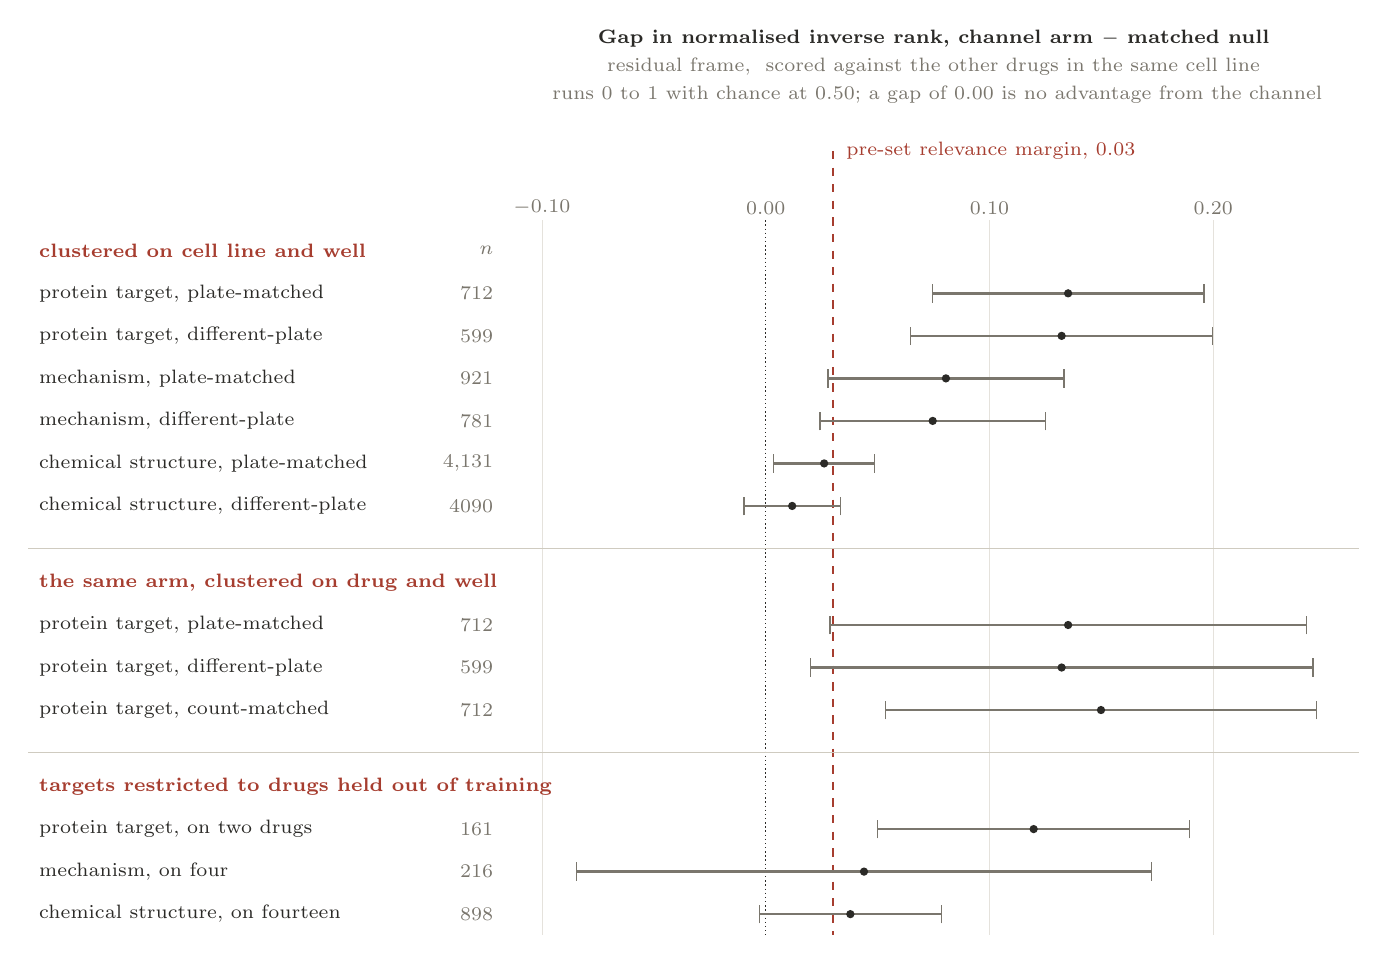
\begin{tikzpicture}[x=108mm, y=5.4mm, font=\small, inner sep=1pt]
  \def\alo{-0.115}\def\ahi{0.265}  % data range of the x axis
  \def\lx{-0.5556}                 % left edge of the row-label column (60.0mm)
  \def\rx{-0.5648}                 % left end of the block rules      (61.0mm)
  \def\ytop{0.72}                  % top of the tick rules and the zero rule
  \def\ybot{-16.1}                 % bottom of the same
  \def\cx{-1.5mm}                  % right edge of the n column, from x=0
  \newcommand{\vx}[1]{{(#1-\alo)/(\ahi-\alo)}}

  % --- one interval row: #1 y, #2 lo, #3 estimate, #4 hi, #5 label, #6 n ---
  % FIX 5: #6 is the row's own count, right-aligned against \cx. A column, not a
  % caption list: twelve counts in prose cannot be matched to twelve rows by eye,
  % and this is how tab:channels carries them one page earlier.
  \newcommand{\gaprow}[6]{%
    \draw[quietink, line width=0.9pt] (\vx{#2},#1) -- (\vx{#4},#1);
    \draw[quietink, line width=0.5pt]
      (\vx{#2},#1-0.22) -- (\vx{#2},#1+0.22);
    \draw[quietink, line width=0.5pt]
      (\vx{#4},#1-0.22) -- (\vx{#4},#1+0.22);
    \fill[ink] (\vx{#3},#1) circle (1.5pt);
    \node[anchor=west, font=\scriptsize, text=ink] at (\lx,#1) {#5};
    \node[anchor=east, font=\scriptsize, text=quietink, xshift=\cx]
      at (0,#1) {#6};}
  \newcommand{\blockhead}[2]{%
    \node[anchor=west, font=\scriptsize\bfseries, text=accent]
      at (\lx,#1) {#2};}

  % --- FIX 1: the axis title. What is measured, in which direction, on what
  % scale, and what zero means. Centred on the data area, not on the drawing.
  % FIX 5 adds the middle line: in which frame, and against which set the score
  % is ranked. Both frames in this document put chance at 0.50, so the scale
  % line below does not distinguish them and cannot be left to do that work.
  \node[anchor=south, font=\scriptsize\bfseries, text=ink] at (0.5,4.70)
    {Gap in normalised inverse rank, channel arm $-$ matched null};
  \node[anchor=south, font=\scriptsize, text=quietink] at (0.5,4.05)
    {residual frame, $\NIR$ scored against the other drugs in the same
     cell line};
  \node[anchor=south, font=\scriptsize, text=quietink] at (0.5,3.40)
    {$\NIR$ runs $0$ to $1$ with chance at $0.50$; a gap of $0.00$
     is no advantage from the channel};

  % --- the scale. FIX 4: the tick set now covers the negative region. ------
  \foreach \v/\t in {-0.10/$-0.10$, 0.10/0.10, 0.20/0.20}{
    \draw[rulegrey!55, line width=0.3pt] (\vx{\v},\ytop) -- (\vx{\v},\ybot);
    \node[anchor=south, font=\scriptsize, text=quietink]
      at (\vx{\v},\ytop+0.06) {\t};}

  % zero, and FIX 2: a numeral, in the same row and register as the others.
  \draw[ink, line width=0.5pt, densely dotted] (\vx{0},\ytop) -- (\vx{0},\ybot);
  \node[anchor=south, font=\scriptsize, text=quietink]
    at (\vx{0},\ytop+0.06) {0.00};

  % the pre-set relevance margin. FIX 3: the rule is carried up to its own
  % callout, 4.4mm of clear space above the tick numerals.
  \draw[accent, line width=0.6pt, dashed] (\vx{0.03},2.35) -- (\vx{0.03},\ybot);
  % (the 1.3mm stand-off is an xshift, not an addition to \vx: \vx expands to
  % a braced pgfmath group and "{...}+0.012" is not a legal coordinate.)
  \node[anchor=west, font=\scriptsize, text=accent, xshift=1.3mm]
    at (\vx{0.03},2.35) {pre-set relevance margin, $0.03$};

  % --- block 1: cell line x well, the axis the gate was run on -------------
  % The n column is headed once, on the first block head's own row: that head is
  % 38.4mm of the 60.0mm column and stops 11mm short of the column, so the two
  % cannot touch. Blocks 2 and 3 keep the same column position and the caption
  % names it, so the head is not repeated over rules it would be read across.
  \blockhead{0}{clustered on cell line and well}
  \node[anchor=east, font=\scriptsize, text=quietink, xshift=\cx] at (0,0) {$n$};
  \gaprow{-1}{+0.0745}{+0.1351}{+0.1958}{protein target, plate-matched}{\num{712}}
  \gaprow{-2}{+0.0648}{+0.1322}{+0.1996}{protein target, different-plate}{\num{599}}
  \gaprow{-3}{+0.0279}{+0.0805}{+0.1332}{mechanism, plate-matched}{\num{921}}
  \gaprow{-4}{+0.0243}{+0.0746}{+0.1249}{mechanism, different-plate}{\num{781}}
  % the flagged count is tab:channels' own \needsaudit{4131}, carried here so the
  % same quantity is not hedged in the table and clean in the figure.
  \gaprow{-5}{+0.0035}{+0.0261}{+0.0487}{chemical structure, plate-matched}%
    {\needsaudit{4{,}131}}
  \gaprow{-6}{-0.0097}{+0.0118}{+0.0333}{chemical structure, different-plate}%
    {\num{4090}}

  % --- block 2: the same target arm, re-clustered on the drug --------------
  % Same records as rows -1, -2 and the count-matched arm, so the counts repeat:
  % re-clustering changes df (38 to 17), never n.
  \draw[rulegrey, line width=0.3pt] (\rx,-7.0) -- (1.00,-7.0);
  \blockhead{-7.8}{the same arm, clustered on drug and well}
  \gaprow{-8.8}{+0.0287}{+0.1351}{+0.2416}{protein target, plate-matched}{\num{712}}
  \gaprow{-9.8}{+0.0199}{+0.1322}{+0.2445}{protein target, different-plate}{\num{599}}
  \gaprow{-10.8}{+0.0536}{+0.1498}{+0.2460}{protein target, count-matched}{\num{712}}

  % --- block 3: targets restricted to drugs held out of training -----------
  % Here the row label counts DRUGS and the column counts conditions; the two
  % are different numbers for the same row, which is why the column earns its
  % place most in this block.
  \draw[rulegrey, line width=0.3pt] (\rx,-11.8) -- (1.00,-11.8);
  \blockhead{-12.6}{targets restricted to drugs held out of training}
  \gaprow{-13.6}{+0.0499}{+0.1197}{+0.1894}{protein target, on two drugs}{\num{161}}
  \gaprow{-14.6}{-0.0846}{+0.0439}{+0.1723}{mechanism, on four}{\num{216}}
  \gaprow{-15.6}{-0.0029}{+0.0378}{+0.0785}{chemical structure, on fourteen}{\num{898}}
\end{tikzpicture}
\caption[The channel gate, by conditioning]{\captiontitle{The gate's verdict is decided
by what the interval is conditioned on, not by where the point estimate falls.}
Every row is residual-frame $\NIR$ scored against the other drugs in the same
cell line: the arm predicts a drug's residual from its annotated neighbours
there, and its matched null draws the same number of partner drugs from that
cell line.
The dot is the estimate, the bar its $95\%$ two-way cluster-robust interval, the
dashed line the pre-set relevance margin of $0.03$ that the gate asks the
\emph{lower} bound to clear. The count beside each row label is the number of
conditions that row scores, not of drugs; the first block's plate-matched counts
are the $n$ of \cref{tab:channels}. The second block re-clusters the same target
arm on the drug, the unit a claim about unseen drugs has to generalise across,
leaving the point estimates untouched; the lower bound now falls short against both
estimand-correct nulls and only the weaker count-matched one clears it. The third
restricts the targets to drugs held out of training. Rows may be read within a
block and not across blocks.}
\label{fig:gate}
\end{fullwidth}
\end{figure}


% ---------------------------------------------------------------------------
\paragraph{What the three channels return} All three arms exclude zero against
their plate-matched nulls on the cell-line axis, so each carries something; what
separates them is whether the effect clears the relevance margin of $0.03$ set
before the gate was run. Clustered on cell line and well, protein target does, at
\ci{+0.1351}{+0.0745}{+0.1958} over $712$ predictions. Mechanism reaches
\ci{+0.0805}{+0.0279}{+0.1332} and falls $0.0021$ short of the margin; chemical
structure reaches \ci{+0.0261}{+0.0035}{+0.0487} and straddles it. Neither of the
two is equivalent to its null, and neither is closed --- inconclusive is a
different verdict from negative, and the distinction is the reason coverage was
printed first.

\paragraph{Which units the interval is clustered on decides the verdict} The
intervals above are two-way cluster-robust on the cell line and the treated well,
as elsewhere in this chapter, which is right for a statement about this
experiment. But the claim a channel is asked to support --- that an \emph{unseen
drug} is reachable through its annotation --- generalises over drugs, and only
$18$ annotated drugs carry the target arm. Wells nest inside drugs rather than
crossing them, so on the drug axis the estimator clusters one-way on the drug and
takes its reference from the drug count (\cref{sec:apparatus-clusters}). Read that
way the target gap is \ci{+0.1351}{+0.0287}{+0.2416}, on $18$ drugs and so
$\mathrm{df} = 17$,
whose lower bound falls $0.0013$ short of the margin; against a null drawing every
partner from other plates it is \ci{+0.1322}{+0.0199}{+0.2445}. Both exclude zero
and neither clears $0.03$. Only the count-matched null clears it on that axis,
\ci{+0.1498}{+0.0536}{+0.2460}, and that is the control already set aside as the
weaker one. Mechanism, which excludes zero on the cell-line axis, spans it on the
drug axis under all three constructions. The axis is chosen by the claim and not
by which interval comes out narrower, so the honest summary is narrower than
\emph{live}.

\paragraph{The population the question is actually about} The channels are scored
on all retained conditions, spanning $94$ drugs, of which $14$ are held out of
training entirely --- the $10$ of the \texttt{unseen\_drug} quota plus four
appearing only in held-out wells. Restricting the targets to those held-out drugs
puts the question where it belongs, and only one channel survives it. Clustered
on cell line and well as everything else here is, the target gap is
\ci{+0.1197}{+0.0499}{+0.1894}; mechanism falls to
\ci{+0.0439}{-0.0846}{+0.1723} and chemistry to \ci{+0.0378}{-0.0029}{+0.0785},
both spanning zero (\cref{fig:gate}, third block). The target arm survives on two
drugs.

\paragraph{What those eighteen drugs are made of} The target arm's $18$ annotated
drugs are almonertinib, amsacrine, cepharanthine, clonidine, elagolix,
gemfibrozil, goserelin, idarubicin, lumateperone, mitoxantrone, neratinib,
norepinephrine, olanzapine, rapamycin, relugolix, temsirolimus, tofacitinib and
tofacitinib citrate. Their mean partner count is $1.19$: of the arm's $712$
predictions, $579$ come from a \emph{single} partner drug and $133$ from two,
against $2.46$ partners for mechanism and $5.00$ for chemical similarity. And
sometimes that partner is an unusually close relative. \texttt{Tofacitinib} and
\texttt{Tofacitinib (citrate)}, the free base and the citrate salt of one drug,
are scored in the same $20$ cell lines and have one partner each; so are rapamycin
and its ester prodrug temsirolimus, in $22$ lines. Neratinib and almonertinib pair
the same way in $20$ lines and are chemically distinct, so the pattern is not only
duplicate chemistry. What the channel establishes is that a same-target neighbour
predicts the drug. That a target \emph{annotation} generalises across a class is
the stronger statement, and testing it would mean dropping the nearest analogue
from each pool.

\paragraph{The two drugs the held-out verdict rests on} They are
\textbf{amsacrine} and \textbf{relugolix}, and since the duplicate-chemistry
pattern above is the obvious objection to them, their pools are worth naming.
Amsacrine is annotated to \texttt{TOP2A} and its partners are doxorubicin,
epirubicin, idarubicin and mitoxantrone; relugolix is annotated to \texttt{GNRHR}
and its partners are elagolix and goserelin. Neither pool contains a salt,
prodrug or stereoisomer of the drug it predicts, so this is not the tofacitinib
case in another guise --- though amsacrine's pool is three anthracyclines and a
close structural analogue of them, which is a drug class and not a duplicate. The
support is $\num{161}$ conditions over $39$ cell lines and $5$ treated wells, $70$
of them amsacrine in two wells and $91$ relugolix in three; the five wells are the
smaller cluster count and are where this interval's $t_4$ reference comes
from.\seealso{\cref{sec:methods-data}: why the smaller cluster count sets the
reference distribution}

\paragraph{Sensitivity to plate matching, measured rather than argued away}
Mechanism partners are co-plated with the target $0.404$ of the time against
$0.362$ for a random draw; elsewhere the diagnostic is negligible, protein target
$0.368$ against $0.366$ and chemical similarity $0.370$ against $0.367$. Under a
third construction drawing every partner from other plates, target and mechanism
keep intervals clear of zero and chemistry's spans it
(\cref{tab:fieldattribution}). Absolute $\NIR$ there is $0.638$, $0.575$ and
$0.499$ against nulls of $0.505$, $0.500$ and $0.487$, so target and mechanism
stay well clear of the $0.50$ chance line while chemistry sits just below it,
where its plate-matched arm already sat. Removing the shared plate moves target
and mechanism by two and seven per cent of their plate-matched gaps, and
attenuates chemistry again. That
construction also changes support and available partners, so the attenuation does
not identify co-plating as its cause.

\paragraph{The ordering is descriptive, and one of its terms is a floor} Target,
then mechanism, then chemistry, under every construction and again on held-out
targets. The target and chemistry intervals do not overlap under any of the three
nulls; each adjacent pair's do, and on the drug axis even the two ends overlap.
The arms differ in support, drug set, partner count and annotation coverage, so
the order does not identify a biological ranking. One correction runs in a known
direction: the residual frame subtracts a plate-local generic, and
\cref{sec:methods-residual} shows that for a co-plated mechanism class part of
that class's own shared programme goes with it, so mechanism's middle position is
a floor rather than an estimate. Below target the two failures differ in kind.
Mechanism's lower bound falls $0.0021$ short, a knife-edge that is not a negative
result in either direction; chemistry's interval is the \emph{narrowest} of the
three, $0.045$ wide against $0.121$ for target, but straddles the margin.

\paragraph{What the lead is, and what bounds it} Two design documents concluded
that unseen-drug generalisation was out of reach, and both inferred it from the
chemical-structure channel alone. The same-target result shows that the inference
from chemistry to every channel was not licensed: the protein a drug hits is what
transcriptional response follows, and structure encodes it only indirectly. Three
things bound the lead. Coverage first --- the arm reaches $18$ of the $94$ scored
drugs. Then scale: a shared property buys a fraction of what the drug itself buys,
the target arm sitting $+0.14$ above chance where a same-drug lookup for a seen
drug sits $+0.41$ (\cref{sec:res-lookup}, on a different condition set, so a
comparison of scale and not a paired one). Then overlap: whether target adds
anything over mechanism is unsettled here, and settling it would need a
leave-one-mechanism-out split, since a held-out drug's mechanism class is
generally still represented in training. What this section measures throughout is
whether the information a channel carries is present in the atlas at all, not
unseen-drug predictive performance, which two drugs cannot establish.


% ===========================================================================
\beatsection{ER}{9}{Which part of the prompt is read remains unresolved}{sec:res-field}

\begin{question}[9]
The previous section asked whether the information an unseen drug would need is
present in the atlas at all. The complementary question is whether the model
reads what it is already handed, and which part of it, the name or the mechanism
line beside it. The instrument swaps one span of the prompt at a time and leaves
every other byte identical. It does not settle the question, and what follows is
why, and what would settle it.
\end{question}

\noindent
The chapter has established that the prediction responds to that information as a
block; it has not established \emph{which} part of it is read. Saying so
precisely matters, because the next step writes itself. Append the protein
targets to the prompt, retrain, and see whether unseen-drug performance rises.
That arm assumes the bottleneck is information availability. Everything in this
chapter points the other way, but the direct evidence is weaker than earlier
drafts claimed.

\paragraph{The instrument, and the one guard it needs} The scramble has until now
replaced the drug name and the mechanism together, so a non-null gap establishes
sensitivity to the combined prompt without attributing it to either span. A field
decomposition swaps exactly one span to the \texttt{opposite} partner, the name
with the mechanism kept, the mechanism with the name kept, and both together. One
guard is essential. If the swap partner happens to share the original's
mechanism, swapping only the mechanism produces a prompt identical to the model's
own and the arm scores exactly zero by construction, which read naively is
indistinguishable from ``the model ignores the mechanism'', the very claim under
test. Such conditions are dropped, which is why the mechanism arm carries fewer
conditions.

\paragraph{What the arms said, and why it does not stand} On the earlier target
build the decomposed arms suggested the prompt sensitivity is carried almost
entirely by the name span. Swapping only the drug name gave $\gap$ of
\ci{+0.0809}{+0.0592}{+0.1010} ($n = 570$); swapping only the mechanism gave
$+0.0091$ [$-0.0174$, $+0.0383$] ($n = 325$); both together gave $+0.1024$
[$+0.0827$, $+0.1236$]. All were scored against the \texttt{opposite}
comparator that \cref{sec:res-generalisation} shows inflates every gap read
against it. They \emph{were} re-run under the corrected evaluation
(\cref{tab:fieldattribution}, Panel B), but the defect survives it, being a
property of the swap partner and not of the target build. The claim that the
model ``reads the name and not the mechanism'' is therefore withdrawn pending
comparators whose own scores are empirically near chance. What the current run
establishes is sensitivity to the combined prompt, with the mechanism field's
contribution unresolved.\corrmark{the name-over-mechanism reading, withdrawn
pending neutral comparators}

% ---------------------------------------------------------------------------
\begin{table}[htbp]
% MARGINALIA: full width, ONE tabular for both panels so the n and interval
% columns align across them. Panel B's rows use the same n and interval columns
% as Panel A (n before the interval, as in Panel A); its span labels run across
% the label and drugs columns. One rule, under Panel A's head; Panel B's head
% row is set off by space. The keyed cell is the one keyed in \cref{tab:channels}.
\caption{\captiontitle{Availability does not establish use.} Panel A shows target and
mechanism retrieval surviving the different-plate null while chemistry does not;
only target clears the relevance margin, and only on the cell-line axis, on an
arm covering $18$ drugs (\cref{sec:res-scope}). Intervals are two-way
cluster-robust over cell line and treated well. Panel B cannot attribute the
combined-prompt effect between name and mechanism, because its two partners lie
on opposite sides of chance ($0.434$ and $0.520$), inflating one gap and
suppressing the other. Comparator-free margins reverse the apparent ordering
($+0.0367$ for name, $+0.0506$ for mechanism), so the split is unresolved pending
comparators whose own scores are empirically near chance. Identical mechanism
swaps are omitted, which is why that row has fewer conditions.}
\label{tab:fieldattribution}
\begin{fullwidth}
\begin{threeparttable}
\begin{tabularx}{\linewidth}{@{}l r r l Y@{}}
\multicolumn{5}{@{}l}{\thead{Panel A: channel availability --- metadata-neighbour
retrieval}} \\
\addlinespace[4pt]
\thead{Channel} & \thead{Drugs (annot./scored)} & \thead{$n$}
  & \multicolumn{2}{l@{}}{\thead{Gap vs plate-matched random null}} \\
\midrule
\key{protein target} & $264$ / $18$ & $712$ & \ci{+0.1351}{+0.0745}{+0.1958} & \\
mechanism (MoA) & $180$ / $26$ & $921$ & \ci{+0.0805}{+0.0279}{+0.1332} & \\
chemical structure & $377$ / $94$ & \needsaudit{4131} & \ci{+0.0261}{+0.0035}{+0.0487} & \\
\addlinespace[10pt]
\multicolumn{5}{@{}l}{\quiet{the same three, against the stricter
\textsc{different-plate} null}} \\
protein target & & $599$ & \ci{+0.1322}{+0.0648}{+0.1996} & \\
mechanism (MoA) & & $781$ & \ci{+0.0746}{+0.0243}{+0.1249} & \\
chemical structure & & $4090$ & \ci{+0.0118}{-0.0097}{+0.0333} & \\
\addlinespace[10pt]
\multicolumn{5}{@{}l}{\thead{Panel B: field use --- one span swapped, every other
byte identical}} \\
\addlinespace[4pt]
\multicolumn{2}{@{}l}{\thead{Span swapped}} & \thead{$n$} & \thead{$\gap$}
  & \thead{Comparator direction (partner $\NIR$)} \\
\addlinespace[6pt]
\multicolumn{2}{@{}l}{drug name, mechanism kept} & $1394$ & \ci{+0.1026}{+0.0625}{+0.1427}
  & inflated ($0.434$) \\
\multicolumn{2}{@{}l}{mechanism, drug name kept} & $738$ & \ci{+0.0303}{-0.0078}{+0.0685}
  & suppressed ($0.520$) \\
\multicolumn{2}{@{}l}{both spans (the standard arm)} & $1394$ & \ci{+0.1139}{+0.0781}{+0.1496}
  & inflated ($0.423$) \\
\end{tabularx}
\begin{tablenotes}
\item Panel A is repeated from \cref{tab:channels} so the two panels can be read
against each other; it is the same measurement, not a second one.
\end{tablenotes}
\end{threeparttable}
\end{fullwidth}
\end{table}

% ---------------------------------------------------------------------------
\paragraph{Why the two panels cannot be added together} Panel A says a channel
carries information in the atlas; Panel B asks whether the model uses what it is
handed. Neither answers the other's question, and an ordering that reverses when
the comparator is removed is not an attribution.

\paragraph{The practical consequence, narrower than earlier drafts drew} The
target-prompt arm is not retired by measurement. It is untested. What argues for
building it carefully is the shape of the failure above. The model's deficit is
not confined to missing information about unseen drugs, because on seen drugs it
covers $13.9\%$ of the distance from chance to the within-well reference, against
a training-only lookup that covers all of it and more (\cref{sec:res-lookup}).
What argues for building it at all is the one thing a lookup cannot do, handle a
drug it has never seen, the regime where \cref{sec:res-scope} finds measurable
transfer through the protein-target channel, on $18$ drugs.

\paragraph{The opportunity is not the part that fails to transfer}
\cref{sec:res-transfer} puts $1 - \Tcoef$ at \ci{44.7\%}{40.7\%}{48.6\%}, and it
is tempting to call that the model's headroom. It is not. That figure is a
shortfall in cross-context similarity, mixing cell line, dose, well and
estimator; it is neither a variance share nor an interaction. With $286$ of $287$
treatments in exactly one well there is no replicate from which to separate a
context-specific remainder from measurement noise, which is why the coefficient
is a disattenuated cross-line cosine and not a fitted variance
decomposition.\seealso{\cref{sec:res-transfer} for the estimator and its five
checks} Whether any of that shortfall is learnable structure and not noise is
separated nowhere here. The opportunity is the unseen drug, and whether the model
can be made to take it is not answered in this chapter.


% 04e-jspace.tex -- the coda of chapter 4, added in thesis_v5. \input at the end
% of 04-Investigation.tex, after 04d-baselines.tex (sec:res-field).
%
% Not a tenth beat, and marked as a coda in words: its own opener says so, the
% chapter opener carries one sentence announcing it, and fig:timeline, the nine
% beats and the six-finding skeleton are unchanged. \beatsection{ER}{0} passes
% beat 0, the value 00-HowToRead gives a section that is not one of the nine.
%
% It takes up the limit that 02-Background.tex (sec:lit-interp) carries forward;
% that scope limit was rewritten in the same version to point here.
%
% THE LEDE IS CLEARED AT THE END. \claimlede stores its text globally and only
% the next \beatsection clears it. This is the last \beatsection in the
% document, so without the \claimlede{} after the claim block its verdict would
% print in every later chapter opener and open chapter 6's claim box.
%
% LAYER NUMBERING. The J-space code indexes transformer blocks from 0; this
% chapter numbers layers as residual-stream depths 1..16 (layer 16 = the last,
% as in tab:workspace). Code blocks 3, 7, 11 are layers 4, 8, 12 here, and the
% lens target, code block 15, is layer 16.
%
% SOURCES. Every number is read from
%   RESULTS_cluster/jspace_frames_v1_analysis/analysis/report.md  (sections 4,5,8,9,10,11)
%   .../analysis/contrasts.csv                                    (full precision)
% except the exploratory ones, computed from phi_pairs.csv and
% secondary_reconstruction.csv by the scripts in tools/jspace_numbers/:
%   ledger.py        relative change, |U| medians, within-checkpoint Spearman
%                    correlations, size-overlap counts, pair-mean phi, readout
%                    and output-change pair means, reconstruction ranges
%   ledger_exact.py  the contrasts.csv rows quoted, at full precision
%   band.py          the shared-size-range comparison at layer 12: drug-minus-
%                    control phi_adj within base drug, averaged over drugs with
%                    both kinds, 95% bootstrap over those drugs (2000, seed
%                    20260912)
%   sizematch.py     per-layer size overlap of drug and control pairs (used for
%                    the no-overlap statements at layers 4 and 8)
% The analysis outputs they read are NOT in the repository (RESULTS_cluster/
% jspace_frames_v1_analysis/ is untracked; phi_pairs.csv alone is 85 MB). The
% scripts find them relative to their own location, and each script's printed
% output is committed beside it as *_out.txt.
% None of the exploratory numbers is in jspace/DESIGN.md, and the prose says so
% each time. Wording follows DESIGN.md section 11: "associated with the residual
% training recipe", phi is "geometric co-location with the lens's token
% directions", a squared norm is a squared norm, the pretrained arm is a
% reference. Checked against the sources by independent read-only reviews in
% three rounds, and the assembled thesis_v5 by a four-reviewer pass; every
% confirmed finding is folded in.
%
% AUDIT. tools/audit.py lists this file in EXTENSION_FILES: it has no v1
% counterpart, so the v1-parity checks A1-A4 do not apply; it is still held to
% margin, opener and strip purity (A5-A7).
% ===========================================================================

\beatsection{ER}{0}{The lens does not single out the drug change}{sec:res-jspace}
% \claimlede must follow \beatsection: \beatsection clears the stored lede.
\claimlede{In the expression frame, at the deepest layer read, the change a drug
swap makes where the answer begins is small and lies along the lens's token
directions barely more than along random ones, and less than a larger control
edit does; the residual recipe is associated with a drug change that reaches the
output, and with more co-location only in the ten-epoch run, where it cannot be
separated from the change's size.}

\begin{question}
A coda to the nine beats, not a tenth. The background chapter took the swap from
the workspace account and left its central claim alone: that a model reads from
a small privileged set of directions, and that content outside it can be richly
represented and still inert. The expression-frame results of this chapter have
that shape, identity written into the activations and barely consulted. The
account's other instrument, the lens that finds such directions, was held back
for here. Point it at the drug. Swap the drug in an otherwise
identical prompt, take the change the swap makes where the answer begins, and
ask how much of that change lies along the directions the lens says the model's
last layer reads.
\end{question}

\noindent
The verdict first. In the expression frame the lens does not single the drug
out. Where the answer begins, swapping the drug moves the layer-$12$ activation
by a median $1.7\%$ of its norm, against $5.4\%$ for swapping the control cell's
sentence, and the directions that code the two prompts capture that small change
barely better than random directions of the same number: $\varphi_{\textrm{adj}}$
is \ci{+0.0013}{+0.0004}{+0.0023}, a $95\%$ drug-node bootstrap interval, as
every interval in this section is unless noted. The drug change lies along the lens's token
directions less than the control change does, though it is also a third of its
size, and in this frame the two share too narrow a range of size to say whether
the ordering would survive at matched size. It moves the model's own first-token
logits about half as far, $39.5$ against $73.4$. Nothing in this geometry singles
the drug out, which fits what \cref{sec:res-mechanism} found by intervention on
the single-cell arm, where the substitution instrument finds nothing.

The residual checkpoints respond to the drug at the output, and the ten-epoch
run's excess of drug over control response is by far the largest. The geometry
separates them from the expression frame in one cell of six, the ten-epoch run
at layer $12$, and there the difference cannot be told apart from the size of
the change it measures. The residual recipe is associated with a larger drug
change that reaches the output. That it moves the drug into the directions the
lens names is \notestablished.

\paragraph{The lens, and the directions it names} Write $h_\ell \in
\mathbb{R}^{d}$ for the residual-stream activation at layer $\ell$ and one
position, with $d = \num{2048}$. The Jacobian lens of Gurnee et
al.~\cite{workspace} summarises how the last layer responds to an earlier one.
Writing $\mathrm{d}h_{16,t}/\mathrm{d}h_{\ell,s}$ for the Jacobian of layer
$16$'s activation at position $t$ with respect to layer $\ell$'s at position $s$,
every other position held fixed, the lens sums it over the positions a source
position can reach and averages over source positions,\gloss{Jacobian
lens}{The average derivative of the last layer's activations with respect to an
earlier layer's.}
\begin{equation}
  J_\ell \;=\; \mathbb{E}_{s}\Big[\, \sum_{t \,\ge\, s}
    \frac{\mathrm{d}h_{16,t}}{\mathrm{d}h_{\ell,s}} \,\Big]
  \;\in\; \mathbb{R}^{d \times d},
\end{equation}
estimated for each checkpoint on $64$ windows of $128$ tokens cut from $32$
calibration prompts on $16$ drugs, none of them an evaluation drug, the first
$16$ positions of each window excluded as sources. Carried back through
$J_\ell$, the output head's row $w_v$ for token $v$, scaled by the final
LayerNorm gain and centred, becomes a direction at layer $\ell$,
\begin{equation}
  d_v \;=\; \frac{J_\ell^{\top} w_v}{\lVert J_\ell^{\top} w_v \rVert},
\end{equation}
along which a change raises token $v$'s logit at the output, to first order.
Over the $\num{50252}$ token ids all four checkpoints share, these are the
lens's token directions: $\num{50252}$ of them in a space of $\num{2048}$
dimensions, of which centring removes exactly one. The same construction with
$J_\ell$ replaced by the identity is the logit lens, kept as a baseline
dictionary $D_0$ with no Jacobian in it. The source layers are $4$, $8$ and $12$.
The lens $J_\ell$ is unrelated to the comparison set $J$ of the reference
apparatus.

\paragraph{The code holds little of any activation} Each activation $h$ is read
at the last prompt token, the colon of \texttt{Response cell:}, where the answer
begins, and coded by non-negative orthogonal matching pursuit: at most $k = 16$
directions chosen greedily, their coefficients refitted jointly under a
non-negativity constraint after each choice, with $k = 8$ and $32$ as
sensitivity. These codes stand in for the workspace account's handful of
concepts active in the J-space at a position. Sixteen directions reconstruct on average between $2.9\%$ and
$5.8\%$ of the activation's squared norm at this position, depending on
checkpoint and layer, and sixteen from the logit lens between $1.9\%$ and
$3.3\%$. That is a sparse reconstruction score,
$1 - \lVert h - \hat{h} \rVert^{2} / \lVert h \rVert^{2}$, not variance
explained, and it fixes how everything below must be read. Most of every
activation lies outside its code, so the numbers are comparisons, a drug edit
against a control edit and one checkpoint against another, never a measure of
how much of the drug is in the workspace.

\paragraph{The pairs} Twenty-four evaluation drugs, four base prompts each, and
every base prompt paired three ways. In a \emph{drug pair} the drug's name and
mechanism line are replaced by another evaluation drug's and nothing else
changes; $84$ of the $192$ drug pairs keep the mechanism text, because the
partner shares it. In a \emph{control pair} the control cell's sentence is
replaced by another real control sentence from the same cell line, the drug
untouched. And each base prompt is paired with itself, run twice. The repeats
return identical activations, so their floor is exactly zero, and no drug or
control pair falls below the exclusion threshold set from the numerical noise of
control pairs. That gives $192$ drug pairs and $96$ control pairs per checkpoint
and layer.

\begin{defn}{Co-location score $\varphi$}
For two prompts $a$ and $b$ that differ in one span, let
$\delta = h_b - h_a$ at one layer, and let $U$ be the union of the directions
chosen to code $h_a$ and $h_b$. Then
\[
  \varphi \;=\; \frac{\lVert P_U\, \delta \rVert^{2}}{\lVert \delta \rVert^{2}},
\]
the share of the change's squared norm that lies in the span of $U$, and
$\varphi_{\textrm{adj}}$ is $\varphi$ minus its mean over $200$ random spans of
$|U|$ directions from the same dictionary. $\varphi_{\textrm{adj}} = 0$ means
the change lies along the directions that code the two prompts no more than
along random ones. It measures geometric co-location with the lens's token
directions, not use and not causal involvement.
\end{defn}

\paragraph{Four checkpoints, and what they license} The
expression-frame checkpoint is the one-epoch single-cell arm of
\cref{tab:trainconfig} ($\num{42198}$ updates). Two residual checkpoints bracket
it in training amount on one training file: the canonical \arm{residual,
repaired} checkpoint of \cref{tab:budget-arms}, after its one epoch
($\num{9231}$ updates), and the ten-epoch run of \cref{sec:app-training}
($\num{92310}$ updates), whose held-out loss is best after its first epoch and
worse at every later one.\seealso{\cref{sec:app-training} for the ten-epoch
run's losses} The pretrained base is a reference only. It has no atomic
\ENDCELL{}, so it reads the same texts under its own token ids, and no claim
rests on it. The checkpoints differ in data, filtering and target format as well
as in updates, so a difference between them is associated with the residual
training recipe and never attributed to the target encoding. The co-location
score is computed the same way in every checkpoint, against no comparison set
and no reference, so unlike the two frames' scores it may be compared across
them; only the first-token logit change inherits the frames' different targets
(\cref{tab:jspace}, note f).

\paragraph{The statistics were fixed before the activations were coded} Pair
scores are averaged within each base drug, then with equal weight over the $24$
drugs. Every drug is both a base and other bases' partner, so intervals come
from a drug-node bootstrap that reweights drugs and weights each drug pair by
both of its members, over $\num{2000}$ resamples. The analysis plan names one
primary family, the six contrasts of each residual checkpoint against the
expression-frame checkpoint on drug pairs at each depth, Holm-adjusted at a
familywise $0.05$. Each is refitted with two half-lenses estimated on disjoint
calibration drugs and called inconclusive if the halves disagree in sign or
differ by more than the contrast itself. A difference may be called
drug-specific only if, once the same contrast on control pairs is subtracted,
the difference-in-differences excludes zero and passes the same gate. The plan
also fixes its sensitivity analyses in advance: other values of $k$, the
logit-lens dictionary, a support capped at $k$ directions, a second read
position at the end of the drug name, and restrictions to pairs whose mechanism
text changes and to drugs absent from residual training.

% ---------------------------------------------------------------------------
\begin{table}[htbp]
% MARGINALIA: full width; caption above at the text width, notes below. Two
% tabulars because Panel C has a different shape from A and B. Every interval
% sits in an l column so it never breaks mid-cell. \key: the one member of the
% primary family that survives Holm.
\caption{\captiontitle{The drug edit lies along the lens's token directions
less than a control edit, except in the ten-epoch run at layer~12, whose drug
change is seventeen times the expression frame's in relative size.} Panel A is
$W$, the drug pairs' $\varphi_{\textrm{adj}}$ minus the control pairs', per
checkpoint and depth: negative means the drug edit is the less co-located.
Panel B is the pre-registered family, each residual checkpoint minus the
expression-frame checkpoint on drug pairs, Holm-adjusted over its six members.
Panel C gives the size of the two edits at layer $12$ and at the output, and the
drug-minus-control difference within the range of size the two kinds share.
$\varphi$ values are $\times 10^{-3}$; unless noted, intervals are $95\%$
drug-node bootstrap intervals over $24$ drugs. The pretrained base is a
reference arm, outside the family.}
\label{tab:jspace}
\begin{fullwidth}
\begin{threeparttable}
\begin{tabular}{@{}l l l l@{}}
\multicolumn{4}{@{}l}{\thead{Panel A: drug edit minus control edit,
  $W$ ($\times 10^{-3}$)}} \\
\addlinespace[4pt]
\thead{Checkpoint} & \thead{Layer 4} & \thead{Layer 8} & \thead{Layer 12} \\
\midrule
expression frame & \ci{-2.3}{-3.4}{-1.3} & \ci{-4.2}{-5.7}{-2.5}
  & \ci{-4.3}{-6.1}{-2.6} \\
residual, one epoch & \ci{-2.9}{-3.8}{-2.0} & \ci{-2.8}{-4.1}{-1.4}
  & \ci{-1.1}{-2.9}{+0.7}\tnote{a} \\
residual, ten epochs & \ci{-2.1}{-3.3}{-0.9} & \ci{-3.6}{-4.6}{-2.6}
  & \ci{+6.3}{+3.9}{+8.7} \\
\quiet{pretrained (reference)} & \quiet{\ci{-3.0}{-3.8}{-2.1}}
  & \quiet{\ci{-0.5}{-1.5}{+0.5}}\tnote{a} & \quiet{\ci{-3.6}{-6.2}{-1.0}} \\
\addlinespace[10pt]
\multicolumn{4}{@{}l}{\thead{Panel B: residual checkpoint minus expression
  frame, drug pairs ($\times 10^{-3}$)}} \\
\addlinespace[4pt]
residual, one epoch & \ci{-0.1}{-1.4}{+1.2}\tnote{a}
  & \ci{-0.5}{-1.9}{+0.9}\tnote{b} & \ci{+1.1}{-0.8}{+3.3}\tnote{b} \\
residual, ten epochs & \ci{-0.4}{-1.9}{+1.1}\tnote{a}
  & \ci{-0.1}{-1.4}{+1.2}\tnote{a} & \key{\ci{+7.0}{+4.4}{+9.5}}\tnote{c} \\
\end{tabular}

\vspace{10pt}
\begin{tabular}{@{}l r r l r r@{}}
\multicolumn{6}{@{}l}{\thead{Panel C: size of the edit, and the difference in
  the shared size range}} \\
\addlinespace[4pt]
& \multicolumn{2}{l}{\thead{Relative change}\tnote{d}}
  & \thead{Drug $-$ control}\tnote{e}
  & \multicolumn{2}{l@{}}{\thead{First-token logit change}\tnote{f}} \\
\thead{Checkpoint} & \thead{drug} & \thead{control}
  & \thead{shared range ($\times 10^{-3}$)} & \thead{drug} & \thead{control} \\
\midrule
expression frame & $1.7\%$ & $5.4\%$ & \ci{-2.5}{-8.0}{+2.4} & $39.5$ & $73.4$ \\
residual, one epoch & $8.7\%$ & $6.9\%$ & \ci{-1.8}{-2.8}{-0.6} & $105.4$ & $81.4$ \\
residual, ten epochs & $30.1\%$ & $6.3\%$ & no shared range & $501.5$ & $118.6$ \\
\quiet{pretrained (reference)} & \quiet{$5.4\%$} & \quiet{$7.9\%$}
  & \quiet{\ci{-2.7}{-4.8}{-0.6}} & \quiet{$98.8$} & \quiet{$129.6$} \\
\end{tabular}
\begin{tablenotes}
\item[a] Inconclusive: the half-lens gate fails, the two half-lenses disagreeing
in sign or differing by more than the estimate itself.
\item[b] Holm-adjusted $p = 1$: no difference from the expression frame is
established.
\item[c] Raw $p = 0.001$, Holm-adjusted $p = 0.006$. Drug-specific under the
plan's rule: the control-pair contrast is \ci{-3.6}{-5.2}{-2.1}, the
difference-in-differences \ci{+10.6}{+7.6}{+13.6}, and both pass the gate. Not
established once the support is capped at eight or sixteen directions, a
sensitivity analysis the plan fixes in advance (see text).
\item[d] Median over pairs of $\lVert \delta \rVert / \lVert h_a \rVert$ at
layer $12$. Descriptive, outside the analysis plan.
\item[e] Layer $12$. Within each base drug, the mean $\varphi_{\textrm{adj}}$ of
its drug pairs minus that of its control pairs, among pairs in the range of
relative size both kinds occupy (bounds fixed from the full sample), averaged
with equal weight over the drugs that have both kinds there: $7$ drugs in the
expression frame, whose shared range, $3.4\%$ to $4.7\%$, holds $15$ of its
$192$ drug pairs; all $24$ in the one-epoch checkpoint and the pretrained
reference. The ten-epoch run's drug and control changes share no range of
size. The interval resamples those drugs, $2{,}000$ times, and ignores the
dependence through partners. Exploratory, outside the analysis plan.
\item[f] Mean L2 norm of the change in the model's own first-token logits over
the shared vocabulary, no lens involved. The first response token means
different things under the two targets, so read drug against control within a
row, not rows against each other across frames.
\end{tablenotes}
\end{threeparttable}
\end{fullwidth}
\end{table}

% ---------------------------------------------------------------------------
\paragraph{Where the expression frame puts the drug} At layers $4$ and $8$ the
drug edit lies along the lens's directions less than the control edit in all
three trained checkpoints (\cref{tab:jspace}, Panel A); the pretrained reference
agrees at layer $4$ and is inconclusive at layer $8$. Those depths decide
nothing, for two reasons. There the expression frame's drug edit is an eighth
and a sixth of its control edit in relative size, and the two share no range of
size at all, so the ordering cannot be separated from size. And the lens says
little there: its linear prediction of how a change reaches the output agrees
with the true change at a Spearman correlation of at most $0.073$ at those
depths, against $0.30$ to $0.63$ at layer $12$.

Layer $12$ carries the argument. There the expression-frame checkpoint's drug
edit sits below its control edit by \ci{-0.0043}{-0.0061}{-0.0026}, as the
pretrained reference's does, by \ci{-0.0036}{-0.0062}{-0.0010}. In pair means
the scale is plain: $1.16\%$ of the drug change's squared norm lies in the span
of its directions against $1.03\%$ for random spans of the same size, where the
control change reaches $1.78\%$ against $1.21\%$. The lens's own prediction points the same way. It predicts how a drug swap moves the output less well than how a
control edit does, by \ci{-0.118}{-0.154}{-0.086} in Spearman correlation.

Whether that ordering is more than size cannot be settled in this frame. The
control edit is three times the drug edit, and the two kinds share only a narrow
range of relative size, $3.4\%$ to $4.7\%$ of the norm, which holds $15$ of the
$192$ drug pairs, from $10$ drugs. Averaged within drug first, as the plan
aggregates, over the $7$ drugs with both kinds in that range, the drug edit sits
lower by \ci{-0.0025}{-0.0080}{+0.0024}, a difference that is \notestablished.
Where the shared range covers every drug, in the one-epoch checkpoint and the
pretrained reference, the drug edit sits lower within it, by
\ci{-0.0018}{-0.0028}{-0.0006} and \ci{-0.0027}{-0.0048}{-0.0006}
(\cref{tab:jspace}, Panel C). In the one-epoch checkpoint the drug changes in that
range are slightly the larger, so the size mechanism below would push the other
way; in the pretrained reference the control changes are still the larger, so
part of its gap could be size. None of these comparisons is in the analysis
plan.

\paragraph{The residual checkpoints respond, and one is placed differently} Both
residual checkpoints move their first-token logits more for a drug swap than for
a control edit, the reverse of the expression frame's
\ci{-33.9}{-43.1}{-20.0}: by \ci{+23.9}{+8.9}{+39.9} after one epoch and by
\ci{+382.9}{+363.5}{+403.6} after ten. That is a drug sensitivity at the first
response token, on a panel of which $17$ of the $24$ drugs are recorded absent
from residual training, and it is larger in the ten-epoch run. Whether it is the
prompt sensitivity \cref{sec:res-encoding} scores, with a different metric and on
trained conditions, is not tested here. At layer $12$ the lens also predicts the
drug swap's effect on the output better than the control edit's in both, by
\ci{+0.094}{+0.066}{+0.120} and \ci{+0.100}{+0.074}{+0.124}.

Where the change lies is another matter. For the canonical one-epoch checkpoint a
difference from the expression frame is \notestablished at any depth: at layer
$12$ it is \ci{+0.0011}{-0.0008}{+0.0033} and at layer $8$
\ci{-0.0005}{-0.0019}{+0.0009}, both with Holm-adjusted $p = 1$, and at layer $4$
the half-lens gate fails. Its own drug-minus-control $W$ at layer $12$ fails the
gate too, so for it the comparison in the shared size range, outside the plan
and without a stability gate, carries no weight on its own. For the ten-epoch run the gate fails at layers $4$ and $8$,
and at layer $12$ the contrast is \ci{+0.0070}{+0.0044}{+0.0095}, raw
$p = 0.001$ and Holm-adjusted $p = 0.006$, the only member of the family to
survive. Its control-pair companion runs the other way,
\ci{-0.0036}{-0.0052}{-0.0021}, so the difference-in-differences is
\ci{+0.0106}{+0.0076}{+0.0136}; it passes its gate, and by the plan's rule the
difference may be called drug-specific. It holds under most of the variations
the plan made. It is \ci{+0.0034}{+0.0016}{+0.0049} with $k = 8$ and
\ci{+0.0146}{+0.0107}{+0.0181} with $k = 32$; the logit-lens dictionary gives
\ci{+0.0102}{+0.0074}{+0.0135}; pairs whose mechanism text changes give
\ci{+0.0078}{+0.0043}{+0.0108}, and the $17$ evaluation drugs recorded absent
from residual training give \ci{+0.0076}{+0.0040}{+0.0113}; read at the end of
the drug name, a position the lens was mostly not fitted at, it is
\ci{+0.0167}{+0.0133}{+0.0197}. Leaving out any one drug keeps it between
$0.0064$ and $0.0073$, and the two half-lenses give $0.0077$ and $0.0070$. The
exception is the plan's own capped support at eight and sixteen directions,
taken up next.

\paragraph{Why that difference cannot be read as the drug moving into the lens's
directions} Three observations are consistent with a size effect rather than
with the drug being placed differently.

Capping the support shrinks it. Keeping only the sixteen directions of $U$ with
the largest summed coefficients, and drawing the null at that size, gives
\ci{+0.0003}{-0.0012}{+0.0018}; coding with $k = 8$ and capping at eight gives
\ci{+0.0001}{-0.0012}{+0.0012}; with $k = 32$ and a cap at thirty-two a smaller
difference survives, \ci{+0.0025}{+0.0003}{+0.0046}, though not with the
logit-lens dictionary, \ci{+0.0016}{-0.0009}{+0.0040}. At the primary $k$ a
difference on the drug pairs is then \notestablished, though the interval still
admits a quarter of the primary estimate. The difference-in-differences stays
positive under the cap, \ci{+0.0046}{+0.0024}{+0.0068}, but through the control
pairs, which sit lower in the ten-epoch run, \ci{-0.0043}{-0.0058}{-0.0028}. The
excess lies in the directions beyond the leading few, which enter $U$ because the
two prompts' codes part company: the ten-epoch run's drug pairs have a median
$|U|$ of $25$ at layer $12$, against $18$ in the expression frame.

It does not need the Jacobian. The logit-lens dictionary, which never applies
$J_\ell$, shows it as strongly, so it is not something the lens's transport
finds.

It tracks size, and size cannot be matched. The ten-epoch run's drug change is a
median $30.1\%$ of the activation's norm, seventeen times the expression frame's
$1.7\%$ and more than three times the canonical checkpoint's $8.7\%$
(\cref{tab:jspace}, Panel C). Within its own drug pairs $\varphi_{\textrm{adj}}$
rises with that relative size at a Spearman correlation of $+0.66$, and with
$|U|$ at $+0.64$; in the expression frame the same two correlations are $-0.006$
and $+0.010$. No range of size is shared. Every one of the ten-epoch run's $192$
drug pairs exceeds a tenth of the activation's norm and $182$ exceed a fifth,
while no expression-frame drug pair reaches a twentieth. Apart from the capped
support, none of these comparisons is in the analysis plan.

One mechanism would produce all three. When a change is a large part of the
activation, the directions chosen to code $h_b$ are partly chosen to code the
change itself, which random directions are not, so $\varphi_{\textrm{adj}}$
rises with the change's relative size whatever the model then does with it. Run
the other way, the same mechanism means that the expression frame's $W$, where
the control edit is the larger, cannot separate placement from size either,
which is why the comparisons in the shared size range are reported, and why they
speak only where that range covers every drug. The plan's rule licenses calling
the ten-epoch difference drug-specific in the narrow sense it defines, that a
control edit does not show it. It does not license reading it as the drug moved
into the set of directions the model reads from.

\begin{scopelimit}[takes up the limit carried from \cref{sec:lit-interp}]
Three limits bound every number above. The lens is applied where it was not
fitted: the last prompt token closes every tail calibration window and is never
used as a source, so its directions there are applied outside the positions they
were estimated at, though at layer $12$ they still predict the true output change
at a Spearman correlation between $0.30$ and $0.63$. The directions are token
directions, not genes: only $8$ of the $946$ panel genes are single whole tokens,
so no reading here is about a gene, and a positive coefficient is not
up-regulation. And co-location is geometry, not use. No workspace vector is
swapped, so the causal claim of the workspace account remains untested, as
\cref{sec:lit-interp} records.
\end{scopelimit}

\begin{claim}
The expression-frame result is negative, and it rests on the pre-registered
measurements at layer $12$. Where the answer begins, the drug swap's change there
is a third of a control edit's in relative size, lies along the lens's token
directions barely more than along random ones and less than that control edit
does, and moves the output about half as far. That fits the single-cell null of
\cref{sec:res-mechanism}; it measures co-location, not use. Whether the drug edit
would sit below a control edit of its own size is not settled in this frame,
where the two kinds share only a narrow range of size. Layers $4$ and $8$ decide
nothing.

The residual result is a statement about the output and a caution about the
geometry. The residual training recipe is associated with a drug change that
reaches the first response token, larger in the ten-epoch run than after one
epoch. Whether the drug is thereby placed in the directions the model reads from
is \notestablished for the canonical checkpoint; for the ten-epoch run the one
difference the family finds is confounded with a change seventeen times the
expression frame's in relative size.
\end{claim}
% Clear the stored verdict: this is the last \beatsection in the document, and
% nothing after it would clear it (see the header).
\claimlede{}


% ===========================================================================
% 05-Limitations.tex.
% ===========================================================================

\chapter{Limitations and future research directions}
\label{sec:limitations}
\framedecl{ER}

\begin{question}
Every measurement in this thesis was made on one atlas, one checkpoint and one
slice of both. Which of its conclusions are properties of the model, and which
are properties of that slice?
\end{question}

\noindent
A limitation is worth writing down when it changes what a number licenses.

% ===========================================================================
\section{What was measured, and on whom}
\label{sec:lim-population}

\paragraph{Only reproducible conditions} A residual that does not reproduce
between two halves of the same well is not a target anything could learn, so the
residual arm trains on the $50.5\%$ of conditions whose residual does reproduce,
$\num{2523}$ of $\num{4999}$ training conditions kept at $\cos > 0.109$, the
$95$th percentile of a null pairing half A of one condition with half B of
another.\gloss{reliability line}{The half-split cosine threshold above which a
condition's residual counts as reproducible.} The model was taught the
empirically reproducible fraction. Split-half retrieval establishes
discriminability of treated populations under this sampling design and cell
budget; it does not establish predictability from untreated input or
learnability.

A reliability filter might be expected to select \emph{toward}
context-in\-de\-pen\-dent conditions and bias the transfer coefficient upward.
It does the opposite. Unfiltered \ci{0.597}{0.563}{0.632}, filtered
\ci{0.553}{0.514}{0.593}; the filtered value is quoted, because disattenuation
is unstable at the very low reliabilities the filter removes.

That calculation's own filter is the inherited $\cos > 0.2$ line, where the
training set uses $0.109$, so the two estimates bracket the trained-on
population without reproducing it. The generation evaluation mismatches
differently again, applying $0.109$ to \texttt{train} and leaving the held-out
splits unfiltered. That one is fundamental and is taken up below.

\paragraph{The splits are scored on different populations} The within-well
split-half precision reference differs sharply across the three splits as
scored, $0.956$ on \texttt{train}, $0.824$ on \texttt{unseen\_combo} and $0.836$
on \texttt{unseen\_drug}. The obvious reading is that held-out conditions carry
less recoverable signal. That reading is wrong.

It is the selection asymmetry noted above. \texttt{train} is drawn from a pool
already filtered at the $0.109$ line, and none of its $300$ scored conditions
falls at or below it, while the held-out splits are unfiltered and still contain
conditions whose two halves disagree outright. Impose the training line on all
three and the references agree at $0.956$, $0.961$ and $0.960$, a spread of
$0.005$ where there had been $0.132$ (\cref{fig:splitref}). Matched on
reproducibility, a held-out condition is as recoverable as a trained one.

% The float that stood here (193-249 of the previous revision) is now
% figs/splitref.tex. It moved out of the section for the same reason the
% other reworked figures did -- the drawing carries 70 lines of its own
% rationale, which does not belong in the prose -- and it lost its
% \begin{fullwidth} on the way: it reserved 174mm, drew 150.2mm, and cost
% this page its margin column to show six numbers the caption already states.
% It now draws 132.9mm inside the 142mm measure.
% ===========================================================================
% splitref.tex -- the within-well split-half reference, as the three splits are
% actually scored and with the resolved +0.1086 reliability line imposed on all
% three.
% \input by Sections/05-Limitations.tex. Compiles against thesis_v2/preamble.tex
% and nothing else. Every number in the drawing is written by
% figs/splitref_numbers.py into figs/fig-splitref.json; run that script if the
% source records ever change, and paste its "TikZ dot values" block below.
%
% STALE GENERATOR -- READ BEFORE RE-RUNNING. splitref_numbers.py:57 hardcodes
% REPRO_LINE = 0.109 and its own comment (:54-56) says 0.109 was chosen because
% it "reproduces all three printed values". That is backwards: the line was
% fitted to the prose rather than taken from the definition, and the prose value
% it was fitted to is the one that is wrong. Panel B below is now drawn at the
% resolved +0.1086 line the document actually defines (see THE LINE). Re-running
% the script as it stands will silently revert this file. Set REPRO_LINE
% = 0.1086 there first, and regenerate figs/fig-splitref.json, which still
% records the superseded 0.109 reconstruction.
%
% v1's version sat inline in Sections/05-Limitations.tex at lines 193-249.
% Four things were wrong with it and are fixed here.
%
%   1. IT PAID FOR FULLWIDTH AND DID NOT USE IT. The old float opened
%      \begin{fullwidth} -- 174mm, and by the preamble's own rule the page
%      carrying one may then carry no margin note -- and drew 150.2mm. It shows
%      six numbers, all six of which its own caption already states, so it was
%      buying 32mm of extra measure to repeat the caption. This draws inside the
%      142mm body measure (see MEASURED below) and that page keeps its margin
%      column.
%
%   2. THE RIGHT-HAND BRACE WAS A DEGENERATE GLYPH. Three values spanning
%      0.956-0.961 on an axis running 0.82-0.98 collapse a
%      decorations.pathreplacing brace to about 1.5pt of path, shorter than its
%      own 3.5pt amplitude, and pgf draws the two halves overlapping: it printed
%      as a stray chevron beside "0.006". A brace that renders as a chevron is
%      worse than no brace. Both spans are now square brackets -- a form that
%      degrades gracefully, so the SAME mark is used in both panels and the
%      reader compares 47.8mm of bracket against 1.8mm of bracket directly.
%      Correspondingly the three converging leaders on the right panel's three
%      near-coincident dots are gone: a single block set hard against the
%      cluster lists all three values in the dots' own top-to-bottom order, so
%      it reads as the cluster magnified rather than as a legend.
%
%   3. NEITHER PANEL SAID WHAT WAS ON THE VERTICAL AXIS. The caption called it
%      "the reference" and the drawing named nothing. There is now a rotated
%      axis title naming the estimator and its frame.
%
%   4. THE TRUNCATION WAS SILENT. The axis runs 0.82-0.98 -- 16 points of a
%      100-point scale -- and that truncation is most of why the 0.132 spread
%      looks dramatic. Both panels share the scale, so the before/after
%      comparison is honest, but the reader has to be told. The axis is drawn
%      BROKEN, with 0.50 (chance, the bottom of the NIR scale's meaningful
%      range) marked below the break, and the caption states the range in words.
%
% GEOMETRY. x and y are both 1mm, so every coordinate below is a millimetre and
% the numbers can be checked against the MEASURED reading. \yv maps a reference
% value onto the axis: \lo..\hi spans \H mm.
%
%   spine            x = 7.5, y = 0 (0.82) .. 58 (0.98)
%   break            gap y = -4 .. 0, two slashes across it, stub -8 .. -4
%   panel A          bracket x = 13, dots x = 36, names from 38.5, values to 66
%   divider          x = 68.5
%   panel B          bracket x = 88, dots x = 91.5, value block from x = 94.5
%   gridlines        stop at x = 94, clear of the value block, uniform length
%
% The two brackets sit on OPPOSITE sides of their dot columns and that is
% deliberate. Panel A's is 47.8mm tall and reads as a measure from anywhere;
% panel B's is 1.8mm and would read as a stray mark if it were the 23mm from
% its dots that panel A's is, so it is set hard against them and its label is
% thrown outward instead. Same mark, same weight, same colour; only the side
% differs, and the two lengths stay directly comparable across the divider.
%
% The two lower dots of panel A sit 0.0127 apart, which is 4.62mm here, against
% a \scriptsize line box of 3.35mm -- so both labels sit at their own dot's
% height and NO leader is needed on the left panel either. That clearance is
% why \H is 58 and not the 52 the old version used.
%
% MEASURED, not estimated. figs/_harness_splitref.tex \input s this file against
% the real preamble, captures the float into a box with \caption and \label
% gobbled, and \typeout s \wd. Reading:
%   tikzpicture  377.33pt = 132.90mm wide, 220.73pt = 77.74mm tall
%   \textwidth   404.03pt = 142.00mm
%   fills 93.4% of the measure, 26.70pt = 9.39mm of slack.
% The build's overfull-hbox gate is 0; this figure contributes none. The
% fullwidth version it replaces drew 150.2mm against a 174mm allowance.
%
% NUMBERS. Panel A is read straight from CANONICAL_NUMBERS.json -> ceilings{}.
% Panel B is reconstructed from re_v3.json -> records[] at repro_cos > 0.1086;
% no file in RESULTS_cluster holds those three values. figs/fig-splitref.json
% carries the full provenance, and is STALE: it still describes the superseded
% 0.109 reconstruction (299 / 394 / 111 kept, train 0.955).
%
% THE LINE. 04c-reencoding.tex:212-213 defines it as the measured null's 95th
% percentile, "+0.109, resolving to +0.1086", and the document is consistent at
% 0.1086, not at 0.109:
%   - 04c:220-221  "Of the 300 scored training conditions ... none falls at or
%                  below the resolved +0.1086." The train minimum repro_cos in
%                  re_v3.json is 0.10892294 -- above 0.1086, BELOW 0.109. At
%                  > 0.109 the figure dropped exactly the condition the text
%                  says is not dropped.
%   - 04c:959      "499 conditions sit below the +0.1086 line" on unseen_combo,
%                  i.e. 396 of 895 kept. The source count of records under
%                  0.1086 is exactly 499; under 0.109 it is 501, giving 394.
%   - 04c:957-958  "train is by construction the reliability-surviving
%                  population", so imposing the line on train must not move
%                  train. At 0.1086 it does not: panel B's train is the same
%                  0.9555006 as panel A's, to the last digit. At 0.109 it moved.
% Recomputed from re_v3.json at repro_cos > 0.1086: kept 300 / 396 / 111, means
% 0.9555006 (train), 0.9605642 (unseen_combo), 0.9597734 (unseen_drug).
%
% TWO NUMBERS THIS FIGURE PRINTS THAT THE PROSE CONTRADICTS. Neither is
% arbitrated here; both are reported upward. The figure does not invent a third
% reading of either.
%   (a) train, panel B. Drawn and printed 0.956, the value the resolved line
%       gives. The prose still prints 0.955 at 04c-reencoding.tex:883 and
%       05-Limitations.tex:224, both inherited from the 0.109 reconstruction.
%       Those two sites need the same correction; they are outside this file.
%   (b) the right-hand spread, printed 0.006. Under the old 0.109 line that was
%       max(rounded) - min(rounded) = 0.961 - 0.955, the raw spread being
%       0.00517. Under the resolved line BOTH conventions give 0.005: the raw
%       spread is 0.0050636, and max(rounded) - min(rounded) = 0.961 - 0.956.
%       So 0.006 is no longer derivable at the line the document defines. It is
%       nevertheless what the prose prints in three places
%       (04c-reencoding.tex:884, 05-Limitations.tex:225 and 03-Apparatus.tex:378,
%       the last a table note in the apparatus chapter), so it is left standing
%       here rather than silently changed to 0.005 -- changing it would put the
%       figure at odds with the prose in three places, and the spread is a
%       claim. FLAGGED, NOT FIXED.
% The left-hand 0.132 is the raw spread rounded and is unaffected.
% ===========================================================================
\begin{figure}[htbp]
% MARGINALIA (06-figures.md): fits the text column; caption in the margin.
\begin{lrbox}{\tvfb}%
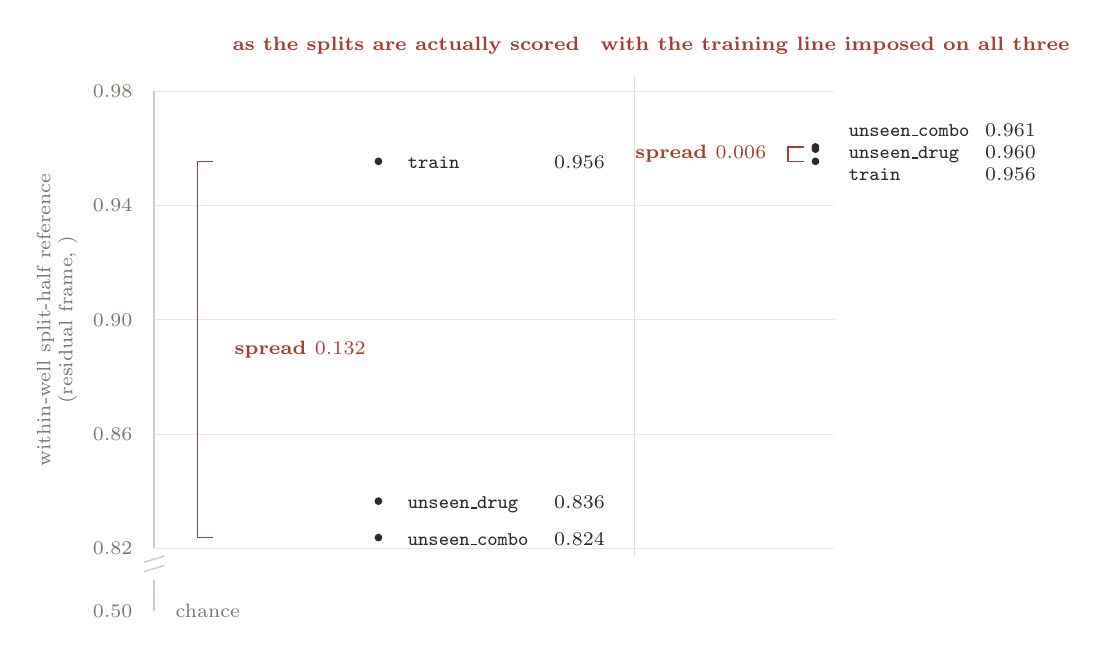
\begin{tikzpicture}[x=1mm, y=1mm, font=\small]
  % --- the constants every coordinate is derived from ----------------------
  \def\lo{0.82}\def\hi{0.98}\def\H{58}
  \newcommand{\yv}[1]{{(#1-\lo)/(\hi-\lo)*\H}}
  \def\ax{7.5}          % spine
  \def\bra{13}\def\dota{36}\def\laba{38.5}\def\vala{66}
  \def\divx{68.5}
  \def\brb{88}\def\dotb{91.5}\def\blk{94.5}
  \def\srf{2}           % bracket serif length, both panels

  \tikzset{
    grid/.style   ={draw=rulegrey!45, line width=0.3pt},
    spine/.style  ={draw=rulegrey, line width=0.5pt},
    tick/.style   ={font=\scriptsize, text=quietink},
    dot/.style    ={fill=ink},
    % text height/depth normalised so a \texttt name and a maths value set at
    % the same y sit on the same baseline; without it Inconsolata's box and the
    % maths box differ by 0.7pt and the three rows print visibly askew.
    lbl/.style    ={font=\scriptsize, text=ink,
                    text height=1.55ex, text depth=0.30ex},
    blk/.style    ={font=\scriptsize, text=ink},
    span/.style   ={draw=accent, line width=0.5pt},
    strong/.style ={font=\scriptsize\bfseries, text=accent}}

  % ---- 1. the shared scale ------------------------------------------------
  % One axis serves both panels; that is the argument, so it is drawn once.
  \foreach \v in {0.82,0.86,0.90,0.94,0.98}{
    \draw[grid] (\ax,\yv{\v}) -- (94,\yv{\v});
    \node[tick, anchor=east] at (\ax-1.5,\yv{\v}) {$\v$};}

  \draw[spine] (\ax,0) -- (\ax,\H);
  % the break, and chance below it. 0.50 is the foot of the NIR scale's
  % meaningful range and it is 32 points below anything drawn, so it is marked
  % past a break rather than pretended onto the plotted span.
  \draw[spine] (\ax,-8) -- (\ax,-4);
  \draw[spine] (\ax-1.3,-3.0) -- (\ax+1.3,-2.2);
  \draw[spine] (\ax-1.3,-1.8) -- (\ax+1.3,-1.0);
  \node[tick, anchor=east] at (\ax-1.5,-8) {$0.50$};
  \node[tick, anchor=west] at (\ax+1.5,-8) {chance};

  \node[rotate=90, anchor=south, font=\scriptsize, text=quietink, align=center]
    at (-1,29) {within-well split-half reference\\(residual frame, $\NIR$)};

  \draw[draw=rulegrey!60, line width=0.4pt] (\divx,-1) -- (\divx,60);

  \node[strong, anchor=south] at (39.5,61.5) {as the splits are actually scored};
  \node[strong, anchor=south] at (94,61.5)
    {with the training line imposed on all three};

  % ---- 2. panel A: the reference as each split is actually scored ---------
  % values: CANONICAL_NUMBERS.json -> ceilings{}
  % Name anchored west at \laba, value anchored EAST at \vala, so the three
  % values line up in a column despite the three split names differing by six
  % characters. Left-setting the whole label leaves them ragged.
  \fill[dot] (\dota,\yv{0.955501}) circle (1.4pt);
  \fill[dot] (\dota,\yv{0.836477}) circle (1.4pt);
  \fill[dot] (\dota,\yv{0.823720}) circle (1.4pt);
  \node[lbl, anchor=west] at (\laba,\yv{0.955501}) {\texttt{train}};
  \node[lbl, anchor=west] at (\laba,\yv{0.836477}) {\texttt{unseen\_drug}};
  \node[lbl, anchor=west] at (\laba,\yv{0.823720}) {\texttt{unseen\_combo}};
  \node[lbl, anchor=east] at (\vala,\yv{0.955501}) {$0.956$};
  \node[lbl, anchor=east] at (\vala,\yv{0.836477}) {$0.836$};
  \node[lbl, anchor=east] at (\vala,\yv{0.823720}) {$0.824$};

  \draw[span] (\bra+\srf,\yv{0.955501}) -- (\bra,\yv{0.955501})
           -- (\bra,\yv{0.823720}) -- (\bra+\srf,\yv{0.823720});
  % 0.889610 and 0.958032 below are the MIDPOINTS of the two spans, used to
  % place each label at the middle of its own bracket. They are geometry, not
  % data, and appear nowhere in fig-splitref.json.
  \node[strong, anchor=west] at (\bra+\srf+1.5,\yv{0.889610}) {spread $0.132$};

  % ---- 3. panel B: the same reference, training line imposed on all three --
  % values: reconstructed from re_v3.json -> records[] at repro_cos > 0.1086,
  % the resolved line of 04c-reencoding.tex:212-213. Kept 300 / 396 / 111.
  % train is 0.955501 -- byte-identical to panel A's train above, because all
  % 300 train conditions clear the line. That identity is the point: the line
  % selects train, so imposing it on train cannot move train.
  \fill[dot] (\dotb,\yv{0.960564}) circle (1.4pt);
  \fill[dot] (\dotb,\yv{0.959773}) circle (1.4pt);
  \fill[dot] (\dotb,\yv{0.955501}) circle (1.4pt);

  % Bracket hard against the dots, opening toward them; label thrown left.
  \draw[span] (\brb+\srf,\yv{0.960564}) -- (\brb,\yv{0.960564})
           -- (\brb,\yv{0.955501}) -- (\brb+\srf,\yv{0.955501});
  % 0.006 is the prose's number, not this panel's: see (b) in the header. The
  % bracket it labels spans 0.0050636, i.e. 0.005.
  \node[strong, anchor=east] at (\brb-1.5,\yv{0.958032}) {spread $0.006$};

  % Three dots 1.8mm apart cannot carry three leaders, and a leader short enough
  % to reach a block set beside them is indistinguishable from a hyphen. So: no
  % leader. One block, hard against the cluster with nothing else within 25mm of
  % it, listing all three in the dots' own top-to-bottom order, so it reads as
  % the cluster magnified rather than as a legend.
  \node[blk, anchor=west] at (\blk,\yv{0.958032})
    {\begin{tabular}{@{}l@{\hspace{2mm}}l@{}}
       \texttt{unseen\_combo} & $0.961$\\
       \texttt{unseen\_drug}  & $0.960$\\
       \texttt{train}         & $0.956$
     \end{tabular}};
\end{tikzpicture}%
\end{lrbox}
\sidecap[The split references, before and after matching]{figure}{\captiontitle{The three
splits do not differ in recoverable signal; they differ in which conditions were
allowed into them.} The vertical axis is the within-well split-half precision
reference --- one half of a condition's cells scored against the other half's
truth, in the residual frame, on the $\NIR$ scale --- and it is
\emph{truncated} to $0.82$--$0.98$, a sixth of the scale; chance is $0.50$,
marked below the axis break and far under everything drawn. Both panels share
that truncated scale, so the two spans may be read against each other. Left,
the reference as each split is actually scored, $0.956$ on \texttt{train}
against $0.824$ and $0.836$ on the held-out splits, a spread of $0.132$. Right,
the same reference with the resolved $+0.1086$ reliability line imposed on all
three, $0.956$, $0.961$ and $0.960$, a spread of $0.006$; at this scale the
three sit inside a bracket two millimetres tall, so they are listed beside the
cluster in
their own order rather than labelled in place. The left-hand spread is a
selection artefact. The markers are bare: no interval is carried for this
reference in the source record, and none is drawn rather than invented.\label{fig:splitref}}

\end{figure}


\emph{Those conditions carry less signal} is therefore not a reason to discount
a held-out result, and this thesis nowhere uses it as one. What survives is
narrower and binding: the matched-population rescore covered the precision
reference only. The model's own arms were never rescored, so where its held-out
scores would sit once the populations agree is not reported here, and the
train-against-held-out comparison of \cref{sec:res-generalisation} inherits the
mismatch --- which matters most for the score that section reports as covering
chance on both held-out splits.

% PLACEMENT ONLY. Eight lines and a framed header, and it was splitting five and
% three across the page turn, so the header sat with half its own text and the
% rest arrived under the running head as an unlabelled fragment. 11 lines is the
% box entire.
\needspace{11\baselineskip}%
\begin{scopelimit}[discharges the limit carried from \cref{sec:res-lookup}]
Three selection rules are in force at once, and no result computed under one of
them may be set beside a result computed under another. A raw score read across
the three splits is not answering the same question on each, because the splits
were filtered by different rules. An absolute $\NIR$ computed with the
comparison set grouped by cell line is not comparable with one computed within
plate. And a per-drug lookup is the bar for a drug that was \emph{seen} in
training and is being asked about a new context: no lookup exists for a drug
that never appeared in training, so that regime keeps its own bar, set in
\cref{sec:res-scope}.
\end{scopelimit}

% ===========================================================================
\section{What the intervals do not cover}
\label{sec:lim-intervals}

\paragraph{No training run was repeated} Seeds in this work move prompts,
partners and resampling. None of them moves the weights. Every arm here was
trained once, from one base checkpoint under identical hyperparameters
(\cref{tab:trainconfig}), so each dissociation this thesis rests on --- the
residual re-encoding against the standard target, and the optimal-transport
target against both --- compares one training run with one training run. A
second run of the same arm under a different data order would land on a
different checkpoint and score differently, and the size of that difference was
never measured here. It is therefore not covered by any interval in this
document: the intervals quantify sampling over conditions, cell lines and wells,
and a between-arm gap of the size reported would survive or fail a training
replication that nobody has run. The ten-epoch diagnostic varies the horizon and
not the seed, so it bounds undertraining and not run-to-run spread. What this
costs is specific rather than general: the \emph{direction} of the re-encoding
effect is corroborated by the token-divergence measurement, which needs no
model at all, but the \emph{magnitude} of every arm-to-arm difference is an
n-of-one comparison.

\paragraph{The intervals omit generation variance} The intervals here are
cluster-robust with each condition's score treated as fixed: two-way over
\emph{cell line} and \emph{treated well} on a $\min(G_{\textrm{line}},
G_{\textrm{well}}) - 1$ Student $t$ reference for the headline gaps, reported
again clustered on the \emph{drug}; multiway dyadic for the transfer
coefficient; a one-way clustered bootstrap, unit named, in a few tables.

They capture between-cluster variance and leave out the variance from sampling
the model's predictions. With four sampled generations per condition at temperature
$0.8$ in the residual-frame arms and eight in the expression-frame ones
(\cref{sec:methods-data}), that source is not negligible, and no across-seed
replication of the generation arms was run, deferred or planned. Every interval
quoted from a generation arm covers the sampling of conditions, cell lines and
wells, and stops there. That includes the within-condition slope regressions of
\cref{sec:res-blind}, \cref{sec:res-epsilon} and \cref{sec:res-generalisation},
whose points are themselves sampled generations, so the comparator-free
instrument this thesis leans on hardest is bounded the same way as the rest.

One measurement \emph{was} repeated across seeds, recorded so it is not mistaken
for the replication that was not run. The activation probe of
\cref{sec:res-mechanism} returned $+0.0197$, $+0.0118$ and $+0.0085$ on three
seeds, each excluding zero. Its spread does not transfer to $\NIR$ and does not
establish a scale for generation variance. Those runs share a checkpoint and
score teacher-forced log-probabilities, so their seed moves the prompts, the
partners and the bootstrap, and leaves both the weights and the sampled
prediction untouched. They are scored on $60$, $240$ and $240$ prompts in that order, so
the largest of the three effects is also the smallest-$n$ one.

\paragraph{Resolution and cross-plate absolutes} Residuals are condition-level
pseudobulks over at least $40$ treated cells, so single-cell heterogeneity of the
response is not modelled in this frame at all; \cref{sec:res-blind} measures what
a single cell can and cannot deliver. Those pseudobulks are then scored against
comparison sets grouped by cell line rather than by plate. The \emph{difference}
$\gap$ is leak-immune, since both arms share the same control cell, but the
absolute $\NIR$ values are a different matter. The plate-scoped generic removes
plate structure in expectation only, and it is estimated from a small plate
group, so some may survive in an individual residual. The rescore that would size
what survives, regrouping the generation-free arms within plate, needs no GPU
time and was not run.

What exists instead is one-sided, and \cref{tab:plateleak} bounds it from
above.\framecue{\Eframe}{the plate-leak audit} In the expression frame with no
generic subtracted, holding the plate constant moves a drug-agnostic mean
baseline from $0.399$ to $0.161$ and the precision reference from $0.625$ to
$0.575$: the yardstick falls with the baseline, so the leak is not an offset one
side of a comparison could be corrected by. Residual-frame absolutes are read
within their own frame and never set beside a within-plate number.

\begin{table}[htbp]
% MARGINALIA: in-column at natural width; caption and both notes in the margin.
\begin{lrbox}{\tvfb}
\begin{tabular}{@{}l r r@{}}
\thead{Predictor (drug-agnostic)} & \thead{cross-plate}
  & \thead{within plate} \\
\midrule
mean baseline & 0.399 & \key{0.161} \\
control-copy & 0.551 & 0.510 \\
\addlinespace[10pt]
\quiet{precision reference (within-well split-half)} & 0.625 & 0.575 \\
fraction of drugs at chance & 43\% & 49\% \\
\end{tabular}
\end{lrbox}
\sidecap{table}{\captiontitle{Expression-frame $\NIR$, the leak audit.} A drug-agnostic mean
baseline more than doubles its score when the plate is free to vary. The
precision reference falls once the plate is held constant, because batch
structure was inflating it too.\label{tab:plateleak}
  \par\addvspace{6pt}A wider diagnostic run than the $n = 606$ tier-2 benchmark the blindness
verdict is stated on, at $n = \num{1163}$ cross-plate and $n = 998$ within
plate. Holding the plate constant costs every condition with no same-plate
comparison set, so the within-plate column is a subset of the cross-plate one
rather than the same conditions rescored.
  \par\addvspace{6pt}Its within-plate figures therefore sit slightly off \cref{tab:allarms},
control-copy $0.510$ against $0.504$, mean baseline $0.161$ against $0.180$,
precision reference $0.575$ against $0.576$.}
\end{table}

% "The similarity is a choice too". States what the frame's choice of SIMILARITY
% costs. (Its companion paragraph on the choice of scored OBJECT was removed as
% duplicating sec:res-transfer.) Sources, all read directly:
%   nir_benchmark.py:13     "expr-NIR : Euclidean distance after decoding ranks
%                            -> expression via linear_model.json"
%   nir_benchmark.py:363-4  d_own = np.linalg.norm(pe - truth_expr[d]) etc.
%   nir_benchmark.py:864    "expression_distance": "Euclidean"
%   residual_eval.py:13     "Similarity = cosine."
%   residual_eval.py:125    def cos(a, b)
% The rescore: RESULTS_cluster/nir_sameplate_profiles.npz, 606 predictions and
% truths over 80 groups, tier2_unseen_drugs, the same support as the frozen
% manifest, scored under the definition of sec:res-metrics with the half-tie
% rule. -||.||_2 gives mean 0.4977 median 0.5000; cosine gives mean 0.5007
% median 0.5000; Spearman 0.6217 between the two per condition; 352/606 move by
% more than 0.10. The Euclidean value reproduces the published 0.498 on the same
% n, which is the only thing validating the rescore, so it is stated.
% The Spearman was re-derived from the same npz under the same half-tie rule
% (scipy spearmanr on the 606 per-condition pairs; Pearson 0.6218, Kendall
% 0.4785 on the same pairs). Restricting to groups of at least three drugs and
% dropping the half-tie rule both return 0.6217; averaging Spearman within
% groups returns 0.5775, a different estimator and not the one quoted.
% NOT RESCORABLE: every local .npz is expression-frame. There is no
% re_*_profiles.npz, so the residual frame carries no such measurement and the
% last sentence says so, which is what stops a reader generalising.
% The sigma instances belong at the definition in 04a-ruler.tex, which already
% parameterises by sigma and already declares the expression instance; this pass
% was scoped to one file, so the residual instance is named here instead.
\paragraph{The similarity is a choice too} $\NIR$ is parameterised by a
similarity $\sigma$ (\cref{sec:res-metrics}), and the two frames instantiate it
differently: the expression frame scores $\sigma(\hat y, y) = -\lVert \hat y - y
\rVert$, the residual frame the cosine. What that choice carries was measured on
the run the blindness verdict is stated on. The same $606$ stored predictions
and truths, the same $80$ comparison groups, tier 2 within plate, were rescored
under both similarities using the definition above, half-tie rule included: the
aggregate reads $0.4977$ under the negated Euclidean distance against $0.5007$
under the cosine, both at chance. The Euclidean value reproduces the published
figure on that support, which is what validates the rescore.

What does not hold across the substitution is the ordering beneath the
aggregate. The two scorings agree per condition at Spearman $0.6217$, and $352$
of the $606$ conditions move by more than $0.10$. That neither strengthens nor
weakens the verdict. A predictor at chance leaves no signal for either
similarity to find, so what separates the two orderings is noise, and the
aggregate stands under both.

Two properties of the published convention belong beside it. A Euclidean
distance is dominated by its largest coordinates, so the high-abundance genes
carry the comparison. And the vectors compared are reconstructions: the
prediction is a cell sentence, decoded to expression through a fitted linear map
before any distance is taken, and that map was fitted for absolute fidelity and
never validated for discrimination (\cref{sec:lit-c2s}). The residual frame
carries no such measurement, because its predictions and truths were not stored
in a form that can be rescored, so nothing is claimed about its sensitivity to
$\sigma$ in either direction.

\begin{scopelimit}[carried into \cref{sec:res-blind} and every per-condition
reading of an expression-frame score]
An at-chance aggregate $\NIR$ in the expression frame holds under either
similarity, negated Euclidean or cosine, on the one run rescored here, tier 2
within plate. Expression-frame aggregates that carry signal were not rescored,
so their standing under $\sigma$ is untested. No per-condition or per-stratum
reading has that standing either: on the run that carries the verdict the two
orderings agree only at Spearman $0.6217$, so no figure below the aggregate may
be presented as independent of $\sigma$. The residual frame carries no such
measurement, so its scores are covered neither way.
\end{scopelimit}

\section{What the unseen-drug arm licenses}
\label{sec:lim-unseen}

Two defects in the unseen-drug arm must be stated. A third, the comparator, was
found and corrected, and \cref{sec:res-generalisation} reports the arm against
the neutral stratum throughout.

\paragraph{The design leaks the drug's class} Holding out a drug does not
remove everything the model knows about it. The prompt contains
\texttt{Mechanism: \{moa\}}, so a held-out drug still arrives with its class
label. The correct design is leave-one-\emph{mechanism}-out.

The leak is measured, and the measurement is not clean. Scrambling the
\texttt{Mechanism} field alone moves the model's $\NIR$ by
\ci{+0.0303}{-0.0078}{+0.0685} ($n = \num{738}$, clustered on drug and well), an
interval containing zero. That understates the channel; it does not bound it,
because this row's swap partner scores $0.520$, above chance, and a comparator
above chance suppresses the gap (\cref{tab:fieldattribution}, Panel~B). A
mechanism-only lookup is the same measurement from the other side and equally
inconclusive. Pooled over the $n = \num{218}$ conditions on which both are
scored, model $-$ \texttt{moa\_lookup} $=$ \ci{+0.044}{-0.048}{+0.135},
clustered two-way on cell line and well, spans zero, so the comparison settles
nothing in either direction.

On \texttt{unseen\_drug}, the split where it would matter, the mechanism lookup
is ahead of the model by $0.099$ on $44$ conditions; in the contrast's reported
direction, model minus lookup is \ci{-0.099}{-0.222}{+0.008}, clustered on cell
line, spanning zero and far too wide to settle anything. That measurement has no
power at exactly the point where the design defect bites. It is not evidence
that the leak is doing work. The design is wrong, the arm cannot say what the
wrongness cost, and its proper use is as an instrument control.

\paragraph{It is underpowered by construction} The half-width on the
\texttt{unseen\_drug} gap is $\pm 0.052$ clustered two-way on cell line and
well, and $\pm 0.073$ clustered on the drug; the smallest effect detectable at
$80\%$ power is $\approx 0.079$. The largest effect the mechanism channel could
deliver is the distance from chance to \texttt{moa\_lookup}, which scores
$0.552$ pooled across splits against a chance value of $0.500$, so $\approx
0.052$. The arm \emph{cannot} detect the largest effect it could plausibly be
measuring (\cref{fig:power}).

% ===========================================================================
% power.tex -- the unseen-drug arm's detection floor against the largest
% effect the mechanism channel could plausibly deliver.
% \input by Sections/05-Limitations.tex, in "It is underpowered by
% construction". Compiles against thesis_v2/preamble.tex and nothing else;
% no \includegraphics, no external file read at build time.
%
% WHY THIS FIGURE EXISTS. The passage it sits in makes its argument out of
% four numbers delivered in four separate sentences (0.052, 0.073, 0.079,
% 0.052-as-largest-effect). The conclusion -- the arm cannot detect the
% largest effect it could plausibly be measuring -- only follows once all
% four are on one scale. On one scale it is a picture: the bar ends before
% the threshold begins.
%
% ---------------------------------------------------------------------------
% EVERY NUMBER DRAWN, ITS SOURCE, AND THE THESIS SENTENCE IT MUST MATCH.
% Sibling power.json records the same list machine-readably.
%
%  threshold (dashed accent rule)      0.07897560995161473
%      RESULTS_cluster/CANONICAL_NUMBERS.json
%          .detection_limit.detectable_at_80pc_power
%      (same object carries .split = "unseen_drug", .n = 199,
%       .observed = 0.45889838436740604, .half_width = 0.05528292696613031;
%       the observed NIR and that half_width are NOT drawn -- this is a
%       difference axis and 0.4589 is an absolute NIR.)
%      Sections/05-Limitations.tex:310-311 "the smallest effect detectable
%      at $80\%$ power is $\approx 0.079$".                        MATCHES.
%
%  bar length                          0.05201514916327314
%      = 0.5520151491632731 - 0.500
%        RESULTS_cluster/CANONICAL_NUMBERS.json .means_all.moa_lookup
%        = RESULTS_cluster/re_v3.json .means.moa_lookup   (identical to 16 sf)
%        chance 0.500 is a definition: both frames are two-alternative
%        retrievals (preamble/frames.tex, Sections/03-Apparatus.tex).
%      Sections/05-Limitations.tex:311-314 "The largest effect the mechanism
%      channel could deliver is the distance from chance to
%      \texttt{moa\_lookup}, which scores $0.552$ pooled across splits
%      against a chance value of $0.500$, so $\approx 0.052$."      MATCHES.
%      0.552 and 0.500 are absolute NIR values and are therefore stated in
%      the caption only; the drawing carries the difference and nothing else.
%
%  point estimate (filled marker)     -0.03148175705606285
%      CANONICAL_NUMBERS.json .splits.unseen_drug.gap
%      = re_v3.json .means.generalization.unseen_drug.gap
%      Sections/05-Limitations.tex:322 \ci{-0.0315}{-0.1049}{+0.0419};
%      Sections/04c-reencoding.tex:791 table row, same estimate twice. MATCHES.
%
%  inner span (thick)  -0.08358077892636565 .. +0.020617264814239943
%      CANONICAL_NUMBERS.json .splits.unseen_drug.gap_ci_line
%      half-width = (0.020617264814239943 + 0.08358077892636565)/2
%                 = 0.052099021870302796  -> 0.052
%      Sections/05-Limitations.tex:308-310 "$\pm 0.052$ clustered two-way on
%      cell line and well". The key "gap_ci_line" is the JSON's own shorthand;
%      tab:generalisation's note says the interval is two-way cluster-robust
%      over cell lines and wells on min(G_line,G_well)-1 = 27 df, so the
%      figure uses the prose's two-way wording.                     MATCHES.
%
%  outer span (thin)   -0.10487258422550776 .. +0.04190907011338206
%      CANONICAL_NUMBERS.json .splits.unseen_drug.gap_ci_drug
%      half-width = (0.04190907011338206 + 0.10487258422550776)/2
%                 = 0.07339082716944491   -> 0.073
%      Sections/05-Limitations.tex:309-310 "$\pm 0.073$ clustered on the
%      drug"; the same interval is printed at 05:322 and at
%      04c-reencoding.tex:791.                                      MATCHES.
%
%  n = 199
%      CANONICAL_NUMBERS.json .splits.unseen_drug.n
%      Sections/04c-reencoding.tex:726 "$\num{199}$ unseen-drug" and the
%      tab:generalisation row "$199$ ($40$; $10$; $28$)".            MATCHES.
%
%  Both intervals are exactly symmetric about the point estimate: the
%  midpoint of gap_ci_line and the midpoint of gap_ci_drug each equal
%  -0.031481757056062853, i.e. .splits.unseen_drug.gap to 16 significant
%  figures. So "point estimate +- half-width" is the intervals themselves and
%  not a symmetrisation of them; nothing is being smoothed here.
%
% DELIBERATELY ABSENT, per the brief: any absolute NIR value inside the
% drawing (0.4589, 0.552, 0.500, 0.8365); any other split; any p-value; any
% legend (both spans are labelled where they end); any gridline.
%
% ---------------------------------------------------------------------------
% GEOMETRY. x is in NIR-difference units at x=383mm, so every coordinate in
% the source below is the datum itself and cannot drift from it by arithmetic
% done here. y is in mm.
%
%   axis          -0.12 .. +0.12   ->  -45.96mm .. +45.96mm   (91.92mm)
%   left column   44mm of flush-right label + 3mm gutter, east edge -48.96mm
%   total width   44 + 3 + 45.96 + 45.96 = 138.92mm, inside the 142.0mm
%                 measure (404.03pt, preamble.tex:793). Measured on the
%                 harness build: see _harness_power.log "HARNESS tikz width".
%   bar tip       0.05201515 * 383 = 19.92mm
%   threshold     0.07897561 * 383 = 30.25mm
%   -> the bar stops 10.33mm short of the rule. That clearance is the whole
%      argument, so it is stated here as a measured length and not judged by
%      eye; at 142mm it is about 7 per cent of the measure and reads at once.
%
%   rows, y in mm   bar      33.5 (rectangle 30.7..36.3)
%                   estimate 13.5 (inner caps 11.1..15.9, outer 12.0..15.0)
%                   axis      0.0, ticks to -1.4, axis title at -7.6
%   detection rule  -1.4 .. 42.5, its label sitting on top of it at 42.6
%   zero rule       -1.4 .. 16.4 -- see note at the draw itself
%
%   MEASURED on the harness build (_harness_power.log):
%     HARNESS textwidth  = 404.02913pt = 142.00mm
%     HARNESS tikz width = 395.70499pt = 139.07mm   <- 2.93mm inside the
%     HARNESS tikz height= 173.09203pt =  60.83mm      measure, 0 overfull
%   and in the whole-thesis build the only Overfull \hbox in main.log is the
%   pre-existing 1.35pt one in figs/fig-frame.tex, not this file.
%
% COLOUR. accent (#0B5394) is spent on exactly two marks, the bar and the
% detection floor, because those two are the comparison the passage makes.
% The observed estimate is ink, the axis and the zero rule rulegrey, all
% descriptive text quietink and every numeral ink. Nothing is told apart by
% colour that is not also told apart by position, weight or shape: the two
% nested spans differ in thickness and in length, not in hue, and the figure
% survives greyscale printing.
% ===========================================================================
\begin{figure}[htbp]
% MARGINALIA (06-figures.md): wider than the 124mm text column, so it
% sits in fullwidth; the caption below spans the text column only.
\begin{fullwidth}\raggedright
\begin{tikzpicture}[
    x=383mm, y=1mm, font=\footnotesize,
    rowlbl/.style  ={text=quietink, align=flush right, text width=44mm,
                     inner sep=0pt, anchor=east, xshift=-3mm},
    ticklbl/.style ={font=\scriptsize, text=quietink, inner sep=0pt,
                     anchor=north},
    axtitle/.style ={font=\scriptsize, text=quietink, inner sep=0pt,
                     anchor=north},
    note/.style    ={text=quietink, inner sep=0pt}]

  % ---- 1. the difference axis ---------------------------------------------
  % Zero, not 0.50, is the reference: this axis carries differences, so the
  % chance level lives inside each quantity's definition and not on the rule.
  \draw[rulegrey, line width=0.5pt] (-0.12,0) -- (0.12,0);
  \foreach \t/\lab in {%
      -0.10/$-0.10$, -0.05/$-0.05$, 0/$0$, 0.05/$+0.05$, 0.10/$+0.10$}{%
    \draw[rulegrey, line width=0.5pt] (\t,0) -- (\t,-1.4);
    \node[ticklbl] at (\t,-2.1) {\lab};}
  \node[axtitle] at (0,-7.6) {difference in $\NIR$\enspace($0$ = no difference)};

  % ---- 2. zero -------------------------------------------------------------
  % The rule stops at 16.4, just under the inner span's label. It does not
  % need to reach the bar row: the bar's own left edge IS x=0 and carries the
  % position up on its own. Running it higher would have to be struck through
  % the "+-0.052" label, which is 46mm wide and must end flush with the inner
  % span's right cap at +0.0206, so it cannot avoid crossing zero. A knocked-
  % out rule reads as a broken line; a shorter one reads as a rule.
  \draw[rulegrey, line width=0.4pt] (0,-1.4) -- (0,16.4);

  % ---- 3. the detection floor ---------------------------------------------
  \draw[accent, line width=0.9pt, dash pattern=on 2.2pt off 1.6pt]
    (0.07897561,-1.4) -- (0.07897561,42.5);
  \node[note, anchor=south east, align=flush right, xshift=-1.0mm]
    at (0.07897561,42.6)
    {smallest effect this arm can\\detect at $80\%$ power,
     \textcolor{ink}{$0.079$}};

  % ---- 4. the largest effect the mechanism channel could deliver ----------
  % It starts at zero because it IS a distance from a null, and it ends
  % where it ends. The dotted arrow is the shortfall: it is drawn without a
  % number on it because the thesis states 0.052 and 0.079 and does not
  % state their difference.
  \fill[accent!20]                (0,30.7) rectangle (0.05201515,36.3);
  \draw[accent, line width=0.7pt] (0,30.7) rectangle (0.05201515,36.3);
  \draw[quietink, line width=0.6pt, dotted, line cap=round,
        -{Latex[length=1.5mm,width=1.3mm]}]
    ([xshift=1.4mm]0.05201515,33.5) -- ([xshift=-0.8mm]0.07897561,33.5);
  \node[rowlbl] at (-0.12,33.5)
    {largest effect the\\mechanism channel\\could deliver\\[0.35ex]
     \textcolor{ink}{$0.052$}};

  % ---- 5. the arm's own estimate, with both cluster keys ------------------
  % Two nested spans, same point estimate, different unit of generalisation.
  % Thin/long = clustered on drug; thick/short = clustered two-way on cell
  % line and well. Told apart by weight and by extent, never by colour.
  % Each label ends FLUSH with the span end it names -- the inner one at its
  % right cap, above; the outer one at its left cap, below -- so the two are
  % separated diagonally and neither needs a legend or a leader line.
  \draw[ink, line width=0.5pt] (-0.10487258,13.5) -- (0.04190907,13.5);
  \draw[ink, line width=0.5pt] (-0.10487258,12.0) -- (-0.10487258,15.0);
  \draw[ink, line width=0.5pt] ( 0.04190907,12.0) -- ( 0.04190907,15.0);
  \draw[ink, line width=1.3pt] (-0.08358078,13.5) -- (0.02061726,13.5);
  \draw[ink, line width=1.0pt] (-0.08358078,11.1) -- (-0.08358078,15.9);
  \draw[ink, line width=1.0pt] ( 0.02061726,11.1) -- ( 0.02061726,15.9);
  \fill[white] (-0.03148176,13.5) circle (2.1pt);
  \fill[ink]   (-0.03148176,13.5) circle (1.6pt);

  \node[note, anchor=south east, align=flush right] at (0.02061726,16.6)
    {$\pm 0.052$ clustered two-way\\on cell line and well};
  % broken over two lines, not one, so that its right edge stops at -0.026
  % and the label clears the zero rule instead of being knocked out of it.
  \node[note, anchor=north west, align=flush left] at (-0.10487258,10.4)
    {$\pm 0.073$ clustered\\on drug};

  \node[rowlbl] at (-0.12,13.5)
    {observed \texttt{unseen\_drug} gap\\($n = 199$)\\[0.35ex]
     \textcolor{ink}{$-0.0315$}};
\end{tikzpicture}
\caption[The detection floor sits above the largest plausible
effect]{\captiontitle{The bar ends before the threshold begins.} Every quantity
here is a difference in $\NIR$ on one scale; no absolute $\NIR$ is plotted.
The dashed rule is the smallest effect the \texttt{unseen\_drug} arm can
detect at $80\%$ power, $0.079$, on the $n = \num{199}$ conditions that arm
scores. The bar is the largest effect the mechanism channel could deliver ---
the distance from chance to the mechanism-only lookup, which scores $0.552$
pooled across splits against a chance value of $0.500$, so $\approx 0.052$ ---
and it stops short of the rule. Beneath it is the arm's own estimate: model
$\NIR$ minus the geometry-defined \texttt{orth} scramble comparator on the
same conditions, $-0.0315$, drawn with the thick span the $\pm 0.052$
half-width clustered two-way on cell line and well and the thin span the
$\pm 0.073$ half-width clustered on the drug. Both cover zero, and the
half-width on the tighter of the two is itself the size of the bar. The arm
is licensed as an instrument control and is not evidence that unseen-drug
transfer is zero: an effect of the largest size the mechanism channel could
deliver would sit inside that same interval, so what it supplies is the
absence of a contradiction rather than a confirmed null.}
\label{fig:power}
\end{fullwidth}
\end{figure}


That cuts both ways, but asymmetrically. As a \emph{control} the arm is not
falsified, since the estimate \ci{-0.0315}{-0.1049}{+0.0419}, clustered on drug,
covers zero. It does not sit \emph{at} zero, being negative and of the same
order as the largest effect the arm could plausibly be measuring, so what it
supplies is the absence of a contradiction. That is why the arm validates the
comparator in \cref{sec:res-generalisation} but cannot argue that unseen-drug
transfer is zero. ``Unseen'' is narrow in a second way too. Pythia-1b's
pretraining is natural-language text in which drug names occur, and the
prompt still supplies \texttt{Mechanism}.

\begin{scopelimit}[carried into \cref{sec:conclusions}]
The \texttt{unseen\_drug} arm is licensed as an instrument control. It is not
evidence that unseen-drug transfer is zero. Its estimate covers zero, but an
effect of the largest size the mechanism channel could deliver would sit inside
that same interval, so what it supplies is the absence of a contradiction rather
than a confirmed null. ``Unseen'' means held out from Tahoe fine-tuning and
nothing wider than that.
\end{scopelimit}

% ===========================================================================
\section{What would settle it}
\label{sec:lim-future}

A limitation earns its place when something could be run to remove it.

\paragraph{The arm to build carefully} The obvious continuation of
\cref{sec:res-scope} is a channel-conditioned prompt that appends protein targets
to the instruction, retrains, and evaluates on a leave-one-mechanism-out split.
We do not recommend building it eagerly. \Cref{sec:res-field} leaves unresolved
which span of the prompt is even read, so a new field would be added to an
instruction whose existing fields are of unmeasured value; and the case against
it does not rest on that anyway, but on the size of the readout deficit. On the
common support the model covers $13.9\%$ of the distance from chance to the
within-well bar that a context-blind lookup covers entirely, and adding a field
to a prompt does not touch that deficit.

Worth building instead is an intervention that makes the drug \emph{causal}
rather than merely present: a learned per-drug modulation of the transformation
from control to treated, so the drug parameterises the computation instead of
sitting in the residual stream as an input the readout can round away. That is a
research architecture, outside the scope of what remained here.

\paragraph{Two channel questions that remain open} Target and mechanism overlap,
so whether target adds anything \emph{over} mechanism is unresolved, and it
matters: the prompt already exposes mechanism, and whether the model reads that
field is itself unsettled. Second, the gate of \cref{sec:res-scope}
measures \emph{similarity transfer}, an unseen drug resembling a seen drug with
the same target. It does not test a \emph{compositional rule}, that a named
target's own pathway moves, which would apply to any drug whose target is named,
including one with no similar drug in training. That claim is the stronger one,
it does not reduce to a lookup, and it is untested.

Protein target clears the relevance margin on the cell-line axis, misses it on
the drug axis against both estimand-correct nulls, clearing it there only
against the weaker count-matched one, and rests on $18$ annotated drugs of which
two are held out; mechanism misses its lower bound by $0.0021$ on the cell-line
axis and spans zero on the drug axis; chemistry's interval straddles the margin
on both. Chemistry attenuates under the different-plate construction, but that
construction also changes support and partner availability, so the attenuation
cannot be assigned causally to co-plating. On its restricted support, same-target
retrieval is the strongest observed lead, and stands only as a direction worth
testing. The binding limitation is coverage: $18$ drugs cannot settle it, and
the experiment that would is a target-annotated panel broad enough to cluster
on.

\paragraph{Unseen cell lines} A cell line never seen with any drug is a
different generalisation axis from the held-out wells tested here, and one the
plating design does not compromise in the same way. It asks whether the control
cell's state is used \emph{compositionally} with the
drug.\seealso{\cref{sec:res-transfer}: $\Tcoef$, and what its complement does
not measure}

The transfer coefficient scopes it only loosely. \ci{44.7\%}{40.7\%}{48.6\%} of
the similarity scale $\Tcoef$ is measured on is not shared across the compared
contexts, and no structure was recovered in that unshared part by tests that do
not settle it. That figure is not a drug$\times$cell-line interaction share,
since it mixes cell line, dose, well and estimator (\cref{sec:res-transfer}), so
it bounds what a per-drug constant leaves on the table without establishing that
a new cell line is the axis the remainder lies along.

No consistent per-line direction was found, so the achievable target on a new
cell line plausibly reduces to recalling the drug's per-drug constant, which a
training-only lookup already does at $0.890$ on held-out wells, the nearest
measured analogue of a new context ($0.913$ pooled, inflated on trained
conditions by the well advantage). The axis is less promising than it appeared,
though the argument is weaker than a coefficient-based one.

\paragraph{Objectives that were considered and rejected} Three training
objectives were designed and then set aside on their own mechanics, recorded so
they are not re-litigated.
\begin{itemize}
  \item \textbf{Reinforcement learning with a contrastive reward.} Its
        per-sequence reward keeps the token-dilution ratio out of the gradient,
        attacking a bottleneck the residual encoding has already lifted ($34.6
        \rightarrow 118.2$ differing tokens at cell-line scope, $120.3$ at the
        plate scope the trained build uses). Its reward optimises similarity to
        the true residual, which \texttt{drug\_lookup} already achieves at
        $0.913$ pooled, $0.890$ on held-out wells. Its best case is convergence
        to the lookup.
  \item \textbf{A differentiable profile-level contrastive loss.} The natural
        construction, $\textrm{score}(g) = \sum_i P(\textrm{token}_i =
        g)\,w(i)$, presumes gene $\approx$ token, but $86.9\%$ of the $\num{946}$
        panel genes share a first sub-token under this tokeniser (mean $3.254$
        BPE tokens per gene, only $8$ single-token). Under teacher forcing the
        target \emph{is} the drug-specific residual, so the true prefix
        identifies the drug within a few symbols and the gradient vanishes at
        the readout solution the loss exists to improve on.
  \item \textbf{Loss re-weighting toward differentially expressed genes.}
        A re-weighted cross-entropy against a single target contains no
        negatives, so nothing forces one drug's prediction to differ from
        another's. It leaves the discrimination failure where it was, and that
        failure is
        what the measurements establish, whether or not the readout is also
        blind to direction specifically, which \cref{sec:res-mechanism} declines
        to establish.
\end{itemize}

\paragraph{One model size, and the smallest one} Every result here comes from a
1B-parameter backbone. C2S-Scale releases checkpoints up to Gemma-2 at 27B, and
we tested none of them, so the most predictable question an examiner can ask,
whether it works if the model is bigger, has no answer in this thesis.

The constraint this work points to is not capacity. The target tokens are
overwhelmingly shared across drugs --- only $17\%$ of them differ between two
drugs in the same cell line under the standard target, against $59\%$ under the
residual encoding at cell-line scope and $60\%$ at the plate scope the trained
build uses (\cref{sec:res-encoding}) --- so very little of the training signal
can carry drug identity. That step is a hypothesis about the optimisation; no
token-level loss or gradient attribution was computed, so no fraction of the
gradient is claimed. A larger model receives the same diluted signal from the
same objective, and re-encoding lifted the effect while leaving
capacity untouched, which points away from capacity without establishing what it
points towards. But the re-encoding changed five things at once, aggregation,
control referencing, sign coding and length among them, and a budget-matched
optimal-transport target lifts the effect too, so \cref{sec:res-encoding}
declines to identify the tokenisation as the constraint that binds.

The genuinely different argument for scale is \emph{prior knowledge}. A 27B
model plausibly knows, as a fact about the world, that a named drug inhibits a
named kinase, which a 1B model may lack. \cref{sec:res-field} leaves
unresolved whether the model uses the \emph{mechanism} field it already has, at
\ci{+0.0303}{-0.0078}{+0.0685} ($n = \num{738}$) with a comparator above chance
suppressing the gap, and real pharmacological knowledge is exactly the case
where that might change. Testing it needs only a low-rank adaptation of a
mid-sized checkpoint. We did not run it, and it is the first thing we would run
with more time.

\paragraph{One epoch, and a thin slice of the atlas} Data scale is the other
half of that question and it is not the same one. Fine-tuning saw
$\num{620564}$ cells, $\num{600000}$ treated and $\num{20564}$ control, drawn
from the roughly one hundred million Tahoe-100M holds, covering $106$ drugs of
its $\approx\num{1100}$, for one epoch at one learning rate
(\cref{tab:trainconfig}). Under a hundredth of the atlas was used, and no arm saw
any cell twice. The diluted-signal argument above survives that: a model trained
on ten times the cells receives the same target strings, so more data of the same
kind does not make the drug easier to see in the loss. The ten-epoch diagnostic
separately rules out undertraining in the optimisation sense, since validation
loss is best at the first epoch and worse at every epoch reported after it.
Neither argument rules out the possibility that a drug must be seen in more
cellular contexts than this sample provides before its response becomes
learnable, and that possibility is \notestablished either way. It is a cheaper
experiment than a larger backbone, and it is not one we ran.

\paragraph{The starting checkpoint was never prepared for this task} We
fine-tune from \texttt{C2S-Scale-Pythia-1b-pt}, whose cell-sentence pretraining
corpus is atlas data alone, CELLxGENE and the Human Cell Atlas, with no
perturbation corpus of any kind, and whose released capabilities do not include
perturbation prediction.

That is why the held-out splits are as clean as they are. A drug withheld here
entered neither the fine-tuning data nor the generic that defines its target,
the split being assigned from metadata before any expression was aggregated, so
no Tahoe perturbation response for it can have been memorised. But the failure
we report is then a failure of \emph{this} starting point, and the fair
follow-up is whether a checkpoint already tuned for perturbation prediction
would behave differently.

Within the C2S-Scale line that question cannot be answered from what is public.
The perturbation-specialised model there is a Gemma-3 4B checkpoint that was not
released. Outside that line it is answerable, and we did not answer it.
Tahoe-x1~\cite{tahoex1} is a perturbation-trained foundation model on this same
atlas, public before this thesis was submitted. It is not a cell-sentence model,
so it does not isolate the representation variable, but it is the obvious
external check on whether a readout failure of this kind survives
perturbation-specific pretraining, and it was not run here. That is a gap in
this work, not a gap in the public record.

Every arm starts from the same base and differs only in the variable under test,
with one material exception, the consensus arm, stopped at roughly $60\%$ of an
epoch with its tier-1 $\NIR$ unscoreable (\cref{tab:trainconfig}). The
\emph{comparisons} between arms are therefore unaffected even where the absolute
level is not, and that arm's null is quoted with the qualification wherever it
is used.

\paragraph{Generality} Everything here is one backbone on one atlas in one
representation. Whether the readout-specificity failure belongs to cell-sentence
models specifically, or to autoregressive conditional generation over
transcriptomes generally, is open. The mechanistic protocol of
\cref{sec:res-used} to \cref{sec:res-mechanism} (purified subspace, removal
gate, positive control, matched-norm swap) transfers unchanged to any model
with an accessible residual stream.

% ===========================================================================
% 06-Conclusions.tex.
% Terminology, load-bearing: held-out treated WELL, trained CONDITION.
% "treated well" is the glossary's form (\glentry, 00-HowToRead:267) and wins
% over "treatment well" everywhere. Never "pairing"; the thesis declines that
% reading.
% ===========================================================================

\chapter{Prompt sensitivity is established; biological transfer is not}
\label{sec:conclusions}
\framedecl{ER}

\begin{question}
Does a cell-sentence language model fine-tuned on this atlas learn what a
particular drug does to a particular cell? The instrument was a chain built in
order: a metric calibrated before it was trusted, controls a drug-blind
predictor cannot pass, and a bar that needs no model at all. The bar was not
cleared.
\end{question}

\noindent
Prompt sensitivity to trained drug names is established; biological transfer is
\notestablished; and nothing built here beats a training-only per-drug lookup on
common support. The win condition was fixed in advance
(\cref{sec:introduction}): a conditional model must beat that lookup, because
only then has its access to the untreated cell supplied something a dictionary
of per-drug averages lacks. A split-half reference cannot stand in for it, since
it cannot separate a drug's characteristic response, which transfers, from this
context's departure from it. That verdict ends a chain, and no isolated point
estimate may leapfrog it.

% ---------------------------------------------------------------------------
\section{The chain, and where each link held}

\paragraph{The metric had to be settled first} Four of five candidate metrics
were saturated by a predictor carrying no drug information: on $\DEdr$ such a
predictor scores $0.9999$. Only $\NIR$ registered known differences in quality,
at a dynamic range fraction of \ci{+0.635}{+0.604}{+0.663}, so it is the only
metric this thesis grades anything on. That is a result before it is an
apparatus choice, and it decides what every later number is allowed to mean.

\paragraph{On that metric the expression-frame checkpoint is drug-blind} It
scores $0.498$ against a within-well split-half reference of $0.576$. On the
stratum where the ranking is provably winnable, a control copying the untreated
cell matches it outright, $0.768$ against $0.766$, a paired contrast of
\ci{+0.002}{-0.026}{+0.028}. Three instruments that fail in different ways agree:
the scramble, the control copy, and a within-condition regression of score on how
unlike the substituted drug is, which returns \ci{+0.0055}{-0.0472}{+0.0582} once
each condition is compared only with itself. That last one matters because its
pooled version returns $+0.0986$ and looks like an effect; the difference between
the two is condition-level structure, not the drug.

\paragraph{The drug is present, and barely consulted} The null is not a failure
to measure. The drug label is decodable from the residual stream at $82\%$
against a $8\%$ chance rate, so it survives into the computation. Ablating the
purified drug subspace costs the output $3.6$ to $18.6$ times a matched-norm
random null, and $9$ to $37\%$ of what ablating cell line costs. The label is
read, and read weakly, which is a different failure from absence and needs a
different repair.

% ---------------------------------------------------------------------------
\section{Re-encoding the target produced a trained-drug effect}

If the drug is in the data and in the activations, the next suspect is the
training target. Two drugs in one context share $83\%$ of their standard target's
top-$200$ tokens; the residual encoding drops that to $40\%$. Aggregating the
target without re-referencing it does not work: of three constructions tried,
none separates from a random-partner scramble, at $+0.014$, $-0.001$ and
$-0.010$, and the optimal-transport arm's within-condition slope is
\ci{-0.0008}{-0.0305}{+0.0290} --- a measured null rather than an absence of
power.

Re-encoding does. On conditions the checkpoint trained on, the residual arm
separates from its own scramble against the geometry-defined \texttt{orth}
partner by $+0.0898$, excluding zero clustered on cell line and well,
\ci{+0.0898}{+0.0382}{+0.1415}, and on drug and well,
\ci{+0.0898}{+0.0291}{+0.1506}.

\paragraph{The comparator is part of the measurement} A prompt replacement is
not automatically a null. The scrambled arm itself scores $0.550$, $0.501$ and
$0.423$ as the substituted drug moves from aligned through orthogonal to
anti-aligned, so a dissimilar lie inflates the apparent benefit of the correct
name. \texttt{Orth} is the one comparator whose own score sits at chance, and it
is the only one whose geometry holds still across the splits the next section
compares.

\paragraph{The gain identifies a package, not a mechanism} Residual encoding
changes aggregation, control referencing, generic subtraction, sign coding and
sequence length at once, and the factorial comparison that would separate them
was not run. Nor is it uniquely responsible: at a matched $1400$-token budget the
optimal-transport arm also clears zero against its orthogonal comparator,
\ci{+0.0292}{+0.0144}{+0.0441}, where its $600$-token estimate spanned zero. A
generation cap can manufacture a null, so any claim about the residual advantage
carries its budget with it.

% ---------------------------------------------------------------------------
\section{The effect does not transfer}

One question is whether the prediction moves when the drug named in the prompt
changes. The other is whether it moves \emph{toward} that drug's response. The
trained-condition effect settles the first for drugs represented in fine-tuning
and leaves the second open.

Conditions in held-out treated wells score $+0.0332$, excluding zero clustered on
cell line and well, \ci{+0.0332}{+0.0069}{+0.0594}, but not on drug and well,
\ci{+0.0332}{-0.0031}{+0.0695} --- and drug is the axis a transferred residual
has to generalise over. That split is largely recombination in any case, with
$30$ of its $34$ drugs and $39$ of its $42$ cell lines in training and $82\%$ of
its conditions pairing a training drug with a training cell line. The model's own
score covers chance on both held-out splits.

\paragraph{What survives the holdout is sensitivity, not accuracy} The
within-condition slope is positive on all three splits and under both
clusterings, \ci{+0.361}{+0.249}{+0.472}, \ci{+0.321}{+0.207}{+0.434} and
\ci{+0.324}{+0.146}{+0.502}, on an instrument that needs no comparator and whose
null is fixed by construction. On the same instrument the single-cell and
optimal-transport arms return nothing. But every point on that line is a
\emph{wrong} prompt, so it shows the model tells wrong answers apart and never
that it produces a right one; and on the unseen-drug split the drugs it names are
overwhelmingly training drugs. The map is coarse and trained-drug-to-residual.

\begin{scopelimit}[discharges the limit carried from \cref{sec:limitations}]
The \texttt{unseen\_drug} arm is read here as an instrument control and not as
evidence that unseen-drug transfer is zero. Its estimate covers zero, but so
would an effect of the largest size the mechanism channel could deliver, so what
it supplies is the absence of a contradiction rather than a confirmed null.
\end{scopelimit}

% ---------------------------------------------------------------------------
\section{Nothing built here beat the lookup}

A per-drug lookup needs no checkpoint, no prompt and no cell
sentence.\seealso{\cref{sec:res-lookup} scores the full ladder through one
pipeline} It predicts a drug's residual as its mean residual in other cell
lines, fitted from training conditions only. On the $\num{1192}$ conditions where
both are defined it scores $0.913$ against the model's $0.549$, with the
within-well reference at $0.857$. Restricted to a single other cell line it still
scores $0.822$, so the win is not an artefact of averaging away noise.

The reading was fixed before the comparison ran: above chance and below the
lookup means the model recovers something of a drug's average residual and adds
no tailoring to the cell line in front of it. That is where it landed. This is
DrEval's finding with a transcriptional vector in place of a scalar potency, and
it sets the bar a conditional architecture has to clear to earn its complexity.

% ---------------------------------------------------------------------------
\section{For an unseen drug, one lead is live and nothing is closed}

No lookup exists for a drug absent from training, so the last gate asks which
shared property could stand in for one. Three channels were tested against a
plate-matched random null, with partners restricted to training conditions.

Protein target clears the pre-set relevance margin clustered on cell line and
well, \ci{+0.1351}{+0.0745}{+0.1958}. Clustered on the drug --- the axis an
unseen-drug claim rides on --- it clears the margin only against the weaker
count-matched null and falls short against both estimand-correct ones. Mechanism
excludes zero on the cell-line axis and misses the margin by $0.0021$; chemistry
straddles it. All three exclude zero, so the two that fail are inconclusive
rather than equivalent to their nulls, and none of the three may be written as
closed.

The lead rests on $18$ target-annotated drugs, two of them held out. Protein
target carries transcriptional signal on that support, and a Leave-Drugs-Out
result is \notestablished by it. Which span of the prompt the model actually
reads is unresolved (\cref{sec:res-field}): the drug name and the mechanism line
beside it were not separated, so a channel-conditioned prompt would add a field
to an instruction whose existing fields are of unmeasured value. The next
experiment needs a target-annotated panel broad enough to cluster on, preferably
with held-out mechanism families, and a prompt whose spans have been told
apart.

% ---------------------------------------------------------------------------
\section{The controls are most of the result}

In a literature where uninformative baselines score well, a negative result is
worth what its controls are worth. Each surviving claim here rests on a control
added after a specific failure: plate-matched comparison sets after a
zero-information baseline improved when plate was free to vary; a swap-distance
sweep after a similar-drug scramble proved weak; a removal gate before any
ablation null; matched-norm injection before any swap was interpreted; condition
intercepts after a pooled slope returned an effect that was not there. Intervals
were clustered on the units that repeat --- cell line, drug and treated well ---
and never on cells.

Claims that failed those controls were withdrawn and the withdrawals recorded
rather than quietly dropped. That record is why the remaining claims can be read
at the strength stated here, and no stronger.

\begin{claim}
On the $\num{1192}$ conditions where both are defined, a training-only per-drug
lookup scores $0.913$ against the model's $0.549$, with the within-well reference
at $0.857$; from a single other cell line it still scores $0.822$. Residual
re-encoding produces a real trained-condition effect against the \texttt{orth}
partner, excluding zero on both clustering axes, and establishes no transfer:
held-out treated wells give an interval that excludes zero on the cell-line axis
and spans zero on the drug axis, and the model's own score covers chance on both
held-out splits. What survives the holdout is the comparator-free slope, which is
sensitivity to the drug named and not accuracy about the drug given. No drug
effect is \shownzero by any instrument here. Of the three channels open to a drug
with no lookup, protein target is live on the cell-line axis and inconclusive on
the drug axis, mechanism and chemistry are inconclusive, and none is closed.
\end{claim}


% v2's measure is narrower than v1's \newgeometry{margin=2.5cm}, and two
% entries carry runs TeX cannot break: ref.bib gives PerturBench the
% Scholar-style journal field {arXiv preprint arXiv:2408.10609}, so the
% identifier is set as an italic journal title with no hyphenation point in it.
% At v2's measure that overflowed by 54.8pt (a second entry overflowed by
% 0.6pt). \emergencystretch buys a final line-breaking pass with extra stretch,
% which is enough to move the identifier down a line. 1em is the smallest value
% that clears both; it adds no underfull lines and costs no page. (The absolute
% count this was first measured against, 166, is long stale -- do not re-derive
% anything from it; check the current log.)
%
% Scoped to this call on purpose. ref.bib is a byte-identical copy of v1's and
% stays that way, so the fix cannot live in the entry; and the shared preamble
% keeps its tighter setting for the body text, where a looser last resort would
% change line breaking in prose that is already settled.
\begingroup
\emergencystretch=1em
\printbibliography[heading=bibintoc]
\endgroup

\appendix
% ===========================================================================
% 07-Appendix.tex -- the apparatus chapter.
%
% main.tex issues \appendix before \include-ing this file, so the \chapter
% below numbers as A and its sections as A.1 ... A.6. Every \label here is
% referenced from the body; none may be renamed.
%
% \framedecl PRECEDES each \section deliberately, exactly as \beatsection
% orders them. Declared after the heading it would write the PREVIOUS
% section's frame into the mark that becomes \firstmark on this section's own
% opening page -- the bug documented in preamble.tex section 5.
%
% NO claim environment in this file, deliberately. Every claim block in the
% thesis sits in the Investigation chapter. An appendix records apparatus; it
% reaches no verdict the body has not.
% ===========================================================================

\chapter{Appendix}
\label{sec:appendix}

\noindent
This appendix holds the apparatus the body leans on but does not stop to
justify. Each section states its verdict in its heading. None is a new result;
several are defects that changed one.

% ===========================================================================
\framedecl{R}
\section{The bespoke estimators recover a planted answer, in both directions}
\label{sec:app-planted}

\begin{question}
Three measurements rest on estimators built for the purpose, and a reader has no
prior reason to trust them. The instrument is a world with a known answer
planted in it, run twice, with the effect and without. All three recover what
was planted, and nothing when nothing was.
\end{question}

\noindent
The weight falls on the null direction.\gloss{planted world}{A synthetic run
with the answer built in, no data, no network, one fixed seed.}

% ===========================================================================
\begin{table}[htbp]
% MARGINALIA: in-column at natural width, so each value sits beside its label;
% the recovered value and its sd are split into two columns so the digits align.
% Group labels are \thead rows; caption in the margin (\sidecap).
% MARGINALIA: caption above at text width (as Table A.2), so nothing in
% this margin can collide with the chapter block or the gloss it pushes down.
\caption[Planted-truth recovery]{\captiontitle{All three estimators recover planted
answers in both directions.} Every row is a synthetic planted-world check, and
none of these numbers comes from the evaluation run or is stored in a result
artifact. The $\Tcoef$ and
$\kappa$-structure rows reproduce from
\texttt{variance\_decomposition.py -{}-selftest}, the channel-gate rows from
\texttt{channel\_gate.py -{}-selftest}. The $\kappa$-structure check must
separate two worlds, within-line consistency exceeding across-line where every
cell line bends what it is given ($+1.17$), the excess vanishing where $\kappa$
is specific to each drug-and-line pairing with no line-level direction
($-0.00$). The lower row of each pair is the null world, the one that rules out
an instrument reporting structure wherever it looks.}
\label{tab:planted}
\begin{lrbox}{\tvfb}
\begin{tabular}{@{}l r@{\hspace{0.4em}}l@{}}
\thead{Planted truth} & \multicolumn{1}{r}{\thead{Recovered}} & \\
\midrule
\multicolumn{3}{@{}l}{\thead{transfer coefficient $\Tcoef$}} \\
\quad $\Tcoef = 1.00$ (fully shared) & $0.999$ & \\
\quad $\Tcoef = 0.70$ & $0.703$ & \\
\quad $\Tcoef = 0.40$ & $0.404$ & \\
\addlinespace[10pt]
\multicolumn{3}{@{}l}{\thead{channel gate, over 24 worlds}} \\
\quad a channel that genuinely predicts & $+0.397$ & (sd $0.029$) \\
\quad a channel carrying nothing & $-0.016$ & (sd $0.091$) \\
\addlinespace[10pt]
\multicolumn{3}{@{}l}{\thead{$\kappa$-structure}} \\
\quad a consistent per-line modulation & $+1.173$ & \\
\quad an idiosyncratic interaction & $-0.002$ & \\
\end{tabular}
\end{lrbox}
\noindent\usebox{\tvfb}\par
\end{table}

\paragraph{What the transfer-coefficient rows do not show} They are a data-free
unit test whose planted world has cell line as its only unshared axis, so
recovery shows the estimator inverting its own generative model and no more. The
canonical run, computed with \texttt{same\_dose\_only=false},
\texttt{loo\_generic=false} and \texttt{repro\_thr=0.2}, lets cell line, dose,
well and estimator noise all enter one number. On synthetic data calibrated to
its gene dimension, cell counts and empirical noise, the estimator returns
$1.001$, $0.747$ and $0.494$ for planted $\Tcoef$ of $1.00$, $0.75$ and $0.50$.

\begin{scopelimit}[carried into \cref{sec:res-transfer}]
Neither the planted rows nor the calibrated repeat licenses reading
$1 - \Tcoef$ as a drug $\times$ cell-line interaction share. The quantity
measures the fraction not shared across the compared contexts, and in the
canonical run those contexts differ in more than cell line.
\end{scopelimit}

\paragraph{Two of these checks changed the instrument} The count-matched null
originally drew random partners from a pool \emph{excluding} the channel's own
selections, which depletes the null of the partners the channel chose and
anti-correlates the two arms. And the useless-channel gap has a standard
deviation of roughly $0.09$ on one small world, so the original validation,
asserting that a single draw fell within $0.10$, tested luck; it now averages 24
worlds. That same variance is why the channel results are gated on a clustered
interval and not on a point estimate.

\paragraph{A third defect was found after the canonical run} The \emph{retrieval}
pool, whose partners' mean residual forms the prediction, was every retained
condition in the cell line except the target's own drug, so a condition held out
of training could enter the prediction for a held-out drug. That is not what
\cref{sec:res-scope} says the gate was intended to do. The code now restricts
the pool to the split's training conditions, logs its size, and never falls back
silently.

The training subset is
\needsaudit{2{,}523} of a retained total logged as
\needsaudit[the split tally sums differently]{4{,}131} conditions, so the old
pool was around $64\%$ larger than it was entitled to be. What makes it a defect
is that a held-out condition could enter at all, which holds at any tally. Every
channel-gate figure in the main text is from the corrected
re-run\corrmark{The channel gate's retrieval pool, repaired and re-run after the
canonical run. \cref{sec:res-scope}}; the planted worlds are unaffected. The
repair moved the channels in no common direction. Target fell, mechanism rose,
chemistry roughly halved, so the pre-fix figures are not quoted alongside them.

% ===========================================================================
% PLACEMENT ONLY. The global \section reservation is 7\baselineskip, sized in
% preamble.tex section 4 for a ONE-LINE heading plus the opener's three-line
% minimum. This title sets on two lines, so 7 lines cleared the test and then
% left the heading, the beat strip and exactly two lines of the lede at the foot
% of the page, with the rest of the lede and the whole VERDICT banner overleaf.
% 15 lines is the two-line heading plus the entire opener, which is how every
% other section in this appendix sets.
\needspace{15\baselineskip}%
\framedecl{E}
\section{The absent-gene convention does not change the answer}
\label{sec:app-convention}

\begin{question}
A predicted cell sentence lists only the genes it expresses, so some panel genes
reach the scorer with no rank and the scorer invents one. Does the invented rank
decide the result? Two conventions were carried side by side. The choice does
not matter, and it never reaches the metric the canonical results rest on.
\end{question}

\noindent
\texttt{worst} assigns absent genes the last rank $G$; \texttt{francesca}
assigns them a fixed middle rank $G/2$. These are the extremes of the plausible
range, so a convention that mattered anywhere would show up between them.

It does not. Spike-in $\DEdr$ reads $0.952$ under the first and $0.954$ under
the second, and no baseline or positive control scored under both moves by more
than $0.01$. That comparison was a one-off diagnostic, never written to an
artifact, so it is a check that was run and not a reproducible result.

\paragraph{How far the convention reaches} It is an input to the rank-based
scores $\DEdr$, $\paneltau$ and \texttt{nir\_rank}, which fills absent genes at
the last rank like the rest.\seealso{\cref{sec:methods-metrics} for why
\texttt{nir\_rank} never entered the graded family} It does not reach the $\NIR$
figures the canonical results rest on, scored by instruments that never receive
the fill. All body figures use \texttt{worst}.

% ===========================================================================
\framedecl{E}
\section{The swap-distance sweep bounds a large effect, and only in one column}
\label{sec:app-sweep}

\begin{question}
If the scramble control swaps in a drug that behaves like the real one, the null
it produces says nothing. The instrument is an earlier, continuous version of
that control, measuring the scramble gap against swap distance. It bounds a
large effect; it does not establish a null, and only one of its two columns
carries that bound.
\end{question}

\noindent
None of these numbers is canonical.\gloss{swap distance}{How far the swapped-in
drug's response lies from that of the drug it replaced.} This is a
separate, earlier run. Its columns are the single-cell and
optimal-transport checkpoints, not the residual arm; it was scored on the
unseen-drug tier of a different evaluation set; and its swap partners were not
restricted to plate, whereas the canonical run draws within plate. Both
artifacts, \texttt{scramble\_sweep\_single.json} and
\texttt{scramble\_sweep\_T2.json}, record \texttt{max\_new\_tokens=1200},
against the $1400$-token budget of the later optimal-transport result.

% ===========================================================================
\begin{table}[htbp]
% MARGINALIA: in-column at natural width; the two model heads set on two lines,
% right-aligned over their columns. Caption ABOVE at the text width, not in the
% margin: the margin caption made the float ~5 lines shorter, which let the
% A.4 opener rise onto the fig:app-sweep-bins page and printed the
% tab:trainconfig scope limit ("recorded above") two pages BEFORE its table.
% \key: the one bin for which an interval is quoted (accent in fig:app-sweep-bins).
\caption[Swap-distance sweep]{\captiontitle{No bin in either model has an interval
excluding zero in this historical $1200$-token run, and the trend correlations
are $\approx 0$.} 200 (drug, swap) pairs over 20 cell lines, $n=40$ per bin. The
single-cell column bounds a large distance effect here. The optimal-transport
column does not carry into the canonical result, where the same checkpoint
clears zero at $1400$ tokens under the within-plate stratified test
(\cref{sec:res-encoding}).}
\label{tab:sweep}
\begin{tabular}{@{}l r r@{}}
\thead{Bin (swap distance)}
  & \multicolumn{1}{r}{\begin{tabular}[b]{@{}r@{}}\thead{single-cell}\\ \thead{model}\end{tabular}}
  & \multicolumn{1}{r}{\begin{tabular}[b]{@{}r@{}}\thead{optimal-transport}\\ \thead{model}\end{tabular}} \\
\midrule
0, nearest (2.75--4.03) & $-0.046$ & $-0.001$ \\
1 (4.03--4.60) & \key{$+0.060$} & $+0.031$ \\
2 (4.60--4.93) & $-0.006$ & $+0.017$ \\
3 (4.93--5.32) & $-0.004$ & $+0.043$ \\
4, farthest (5.32--6.25) & $-0.019$ & $-0.005$ \\
\addlinespace[10pt]
trend, corr(distance, $\gap$) & $+0.051$ & $+0.012$ \\
\end{tabular}
\end{table}

% ===========================================================================
\begin{figure}[htbp]
% MARGINALIA (06-figures.md): fits the text column; caption in the margin.
\begin{lrbox}{\tvfb}%
\begin{tikzpicture}[x=21mm, y=1mm, font=\small]
  % The DOT carries the value, always. Four of the five gaps sit within a few
  % thousandths of zero, so their labels are lifted to one clear row and tied
  % back with a leader. Nothing is repositioned that could be misread as a
  % different number. There are no numeric axis ticks; each strip carries the
  % one reference line its own quantity has, zero for the gap above and chance
  % for the $\NIR$ below, and the lower strip is a DIFFERENT QUANTITY, which is
  % what the divider between the two strips is there to say.
  \def\ur{180}                     % upper strip, mm per unit of the gap
  \def\lz{-52}\def\ls{63}          % lower strip, origin and mm per unit
  \def\lchance{\lz+(0.5-0.326)*\ls}% -41.04mm: $\NIR = 0.50$ on the lower strip
  \newcommand{\liftedgap}[2]{%
    \fill[ink] (#1,{#2*\ur}) circle (1.5pt);
    \draw[rulegrey, line width=0.3pt] (#1,{#2*\ur}) -- (#1+0.08,-14);
    \node[anchor=west, font=\scriptsize, text=ink] at (#1+0.10,-14) {$#2$};}
  % The value label carries a white backdrop because the chance rule runs
  % under this strip: the nearest value, 0.497, sits ON that rule, and a dotted
  % line through its digits is the one way this label could be misread.
  \newcommand{\nirdot}[2]{%
    \fill[quietink] (#1,{\lz+(#2-0.326)*\ls}) circle (1.3pt);
    \node[anchor=west, font=\scriptsize, text=quietink, fill=white, inner sep=1pt]
      at (#1+0.06,{\lz+(#2-0.326)*\ls}) {$#2$};}

  % === upper strip, the scramble gap in the single-cell column ==============
  \node[anchor=west, font=\scriptsize\bfseries, text=accent]
    at (-0.42,29) {$\gap$, single-cell column};
  \draw[ink, line width=0.5pt, densely dotted] (-0.42,0) -- (4.40,0);
  \node[anchor=west, font=\scriptsize\itshape, text=ink] at (4.42,0) {zero};

  % the one bin for which an interval is quoted, drawn as an interval
  \draw[accent!55, line width=1.6pt] (1,{-0.002*\ur}) -- (1,{0.124*\ur});
  \fill[accent] (1,{0.060*\ur}) circle (1.6pt);
  \node[anchor=west, font=\scriptsize, text=accent]
    at (1.08,{0.060*\ur}) {$+0.060$};

  \liftedgap{0}{-0.046}
  \liftedgap{2}{-0.006}
  \liftedgap{3}{-0.004}
  \liftedgap{4}{-0.019}

  % === the divider IS the argument, two quantities, two scales, one x =======
  \draw[rulegrey, line width=0.4pt] (-0.42,-20) -- (4.40,-20);

  % === lower strip, the model's own score, which drifts =====================
  \node[anchor=north west, font=\scriptsize\bfseries, text=quietink]
    at (-0.42,-23) {the model's own $\NIR$ (expression frame) in the same bins,
      on its own scale};
  % The chance line at 0.50 is drawn on EVERY $\NIR$ axis, always
  % (figs/style_v2.py): omitting it, or implying it through the extent of the
  % marks, lets a reader infer a scale that does not exist. Three of these five
  % values sit below it and two above, and nothing else in the drawing says so.
  % Same dotted ink as the zero rule above, because the two are the same kind of
  % thing -- each strip's own single reference -- and drawn BEFORE the marks so
  % the data reads on top of it.
  \draw[ink, line width=0.5pt, densely dotted]
    (-0.42,{\lchance}) -- (4.40,{\lchance});
  \node[anchor=west, font=\scriptsize\itshape, text=ink]
    at (4.42,{\lchance}) {chance};
  \nirdot{0}{0.497}
  \nirdot{1}{0.612}
  \nirdot{2}{0.523}
  \nirdot{3}{0.401}
  \nirdot{4}{0.326}

  % === the one axis the two strips share ====================================
  \foreach \i/\lab in {0/nearest, 1/{}, 2/{}, 3/{}, 4/farthest}{
    \node[anchor=north, font=\scriptsize, text=quietink, align=center]
      at (\i,-58) {\i\\\lab};}
\end{tikzpicture}%
\end{lrbox}
\sidecap[Swap distance and the scramble gap]{figure}{\captiontitle{The one borderline value
sits in an inner bin, and the drift that could have faked a trend is in a
quantity the gap cancels.} Upper strip, the scramble gap in the single-cell
column across the five swap-distance bins of \cref{tab:sweep}; the bar marks the
only bin for which an interval is quoted, \ci{+0.060}{-0.002}{+0.124}. A genuine
dissimilarity effect would be monotone and peak at the right-hand edge, and the
one value approaching zero from above is the second bin of five. Lower strip,
the model's own $\NIR$ in those bins ($0.497$, $0.612$, $0.523$, $0.401$,
$0.326$), falling overall but not monotonically, because drugs far from
everything populate the far bins. The strips are different quantities on
different scales; $\gap$ uses the same drug on both arms, so that drift cancels.
Neither strip is canonical (\texttt{max\_new\_tokens=1200}, $n=40$ per bin).\label{fig:app-sweep-bins}}

\end{figure}

\paragraph{What the sweep can and cannot support} $n=40$
per bin gives half-widths of $0.06$--$0.10$ in the single-cell column and
$0.03$--$0.06$ in the optimal-transport column, so the sweep excludes a large
effect without establishing a
null.\seealso{\cref{sec:methods-controls} for the stratified scramble
that replaced this design} The later budget-matched result withdraws the
optimal-transport column as evidence of a null, that verdict being
generation-budget dependent and non-null at $1400$ tokens
(\cref{sec:res-encoding}).\corrmark{The optimal-transport column of this sweep,
withdrawn as evidence of a null. \cref{sec:res-encoding}}

\begin{scopelimit}[carried into \cref{sec:res-blind}]
Only the single-cell column remains a bound from this earlier design, and it is
a bound and not a null. At this sample size it excludes a large dissimilarity
effect and leaves a small one open. The optimal-transport column has been
withdrawn as evidence of a null, so nothing in this section rests on it.
\end{scopelimit}

% ===========================================================================
\framedecl{-}
\section{Undertraining is excluded as a trivial explanation, not as a general one}
\label{sec:app-training}

\begin{question}
A negative result invites the objection that the model was simply not trained
enough, and that objection deserves an answer from the logs. Two instruments
give one, what the loss was doing while the learning rate was still large, and
what a much longer schedule does to held-out cross-entropy. Under this schedule,
longer optimisation does not rescue it.
\end{question}

\begin{table}[htbp]
% MARGINALIA: full width at natural width (~147mm, too wide for the 124mm
% column without wrapping three columns); the caption (too long for the margin)
% sits above at the text width. The Note column stays: its entries are
% row-specific cells, two of them empty.
% \key: the consensus arm's truncated schedule, the cell the caption turns on.
\caption[Training configuration]{\captiontitle{One base checkpoint, one
hyperparameter set, five arms differing only in target.} Learning rate
$10^{-5}$, batch size 1, gradient accumulation 16, maximum length 8192, bf16,
weight decay 0.01, warmup ratio 0.03 throughout. The consensus arm stopped early
on a flat loss, so it is the $\varepsilon$-ladder's weakest-evidenced endpoint,
and at the residual arm's generation budget against a neutral partner the
optimal-transport endpoint is not null either (\cref{sec:res-encoding}); outside
\cref{tab:epsilon} the ladder's negative rests on the single-cell endpoint
alone. These five arms (\texttt{single\_cell}, \texttt{consensus},
\texttt{ot\_T2}, \texttt{residual}, \texttt{residual\_holdout}) are also the
complete family over which the identity test of \cref{sec:res-mechanism} takes
its multiplicity correction, five arms by up to seven depths and $26$ measured
tests, the family behind the $q$-values quoted there. One qualification attaches
to the residual row. Its step count is the rebuilt target build's, on which the
canonical behavioural results are scored, while the identity test of that arm
ran on the earlier target build.}
\label{tab:trainconfig}
\begin{fullwidth}
\begin{tabular}{@{}l l l l@{}}
\thead{Arm} & \thead{Target} & \thead{Training} & \thead{Note} \\
\midrule
single cell & the observed treated cell & 1 epoch & \\
consensus & group pseudobulk & \key{$\approx$ 60\% of an epoch}
  & tier-1 $\NIR$ unscoreable \\
optimal transport (T2) & barycentric, $\varepsilon{=}0.5$
  & 1 epoch, 23{,}842 steps & \\
residual & signed residual & 1 epoch, 9{,}231 steps
  & rebuilt build's step count \\
residual (holdout) & as above, 738 withheld & 1 epoch & \\
\end{tabular}
\end{fullwidth}
\end{table}

% ===========================================================================
% MOVED HERE from the end of A.4 -- PLACEMENT ONLY. Not one character of the
% figure, its caption or its numbers was changed; only the point of declaration.
%
% It is declared AHEAD of tab:trainconfig deliberately. Both are section-opening
% material, but the figure has a \cref in this section and the table does not:
% tab:trainconfig is a lookup cited only from chapters 4 and 5, so it is free to
% take the later float slot while the figure takes the one nearer its reference.
%
% MEASURED, in this order:
%   declared at the end of A.4 (as it was): float lands p.118, two pages past
%     its \cref on p.116, and the room it leaves under itself on p.118 fits the
%     two \Large lines of the A.5 heading and nothing else -- the heading is
%     stranded at the foot of the page with zero lines below it.
%   declared next to its \cref but still after the table: float still lands
%     p.118. The table, declared earlier, holds the only top slot on p.117.
%   \needspace{10\baselineskip} on the A.5 heading: BYTE-IDENTICAL PDF. It
%     cannot work from the heading's side -- \needspace tests
%     \pagegoal-\pagetotal in the main vertical list, before the deferred float
%     has been contributed to the page, so it reads a full page of room and
%     passes. The float is the cause, so the float is what moves.
%   declared here: float lands p.117, one page from its \cref, and the A.5
%     heading is no longer orphaned. Cost: one page, and p.117 sets the figure
%     with two lines of text under it.
\begin{figure}[htbp]
\begin{fullwidth}
\raggedright
% drawn at 174mm by thesis_v2/figs/training.py; no width= key, so it is placed
% at scale 1.0 and its type prints at the point sizes it was set in.
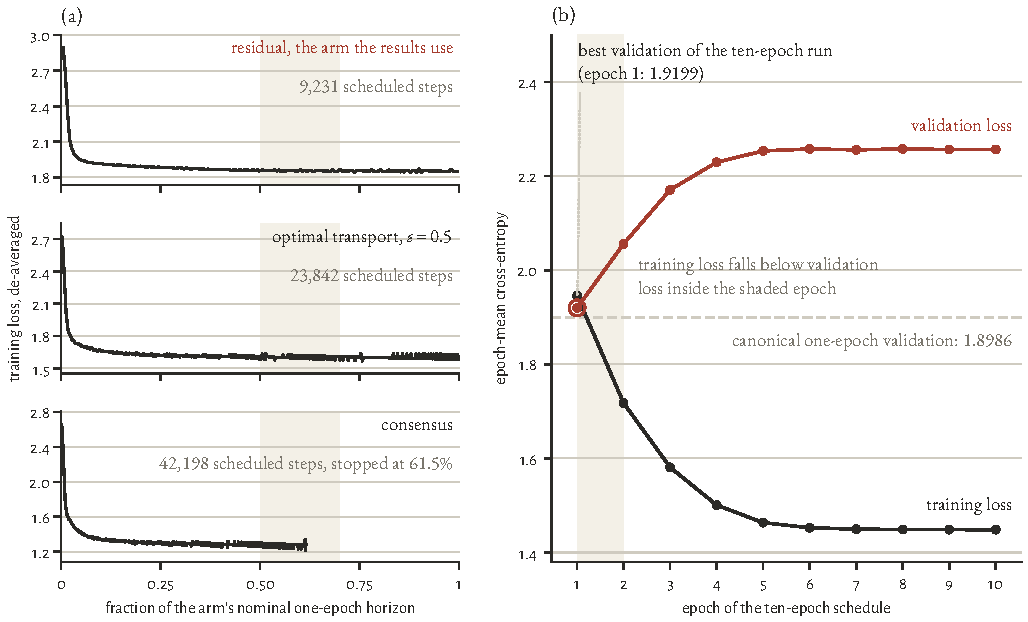
\includegraphics{fig-training}
\caption[The short-run arms flatten; a longer schedule
overfits]{\captiontitle{The canonical short-run arms flatten, while a
separate longer residual schedule overfits on held-out cross-entropy.}
(a) De-averaged training loss against fraction of the nominal one-epoch horizon,
three target constructions, each on \emph{its own} $y$-axis: absolute losses are
not comparable between arms because their target strings differ, so no shared
scale is offered. The residual and optimal-transport arms complete their epoch;
consensus was scheduled for one but terminated by the wall-clock at $61.5\%$,
where its line stops. Three superseded residual builds are omitted, as is the
single-cell arm, whose training log was not retained. Every arm runs a cosine
schedule annealing to $\approx 0$; the shaded band marks $50$--$70\%$ of the
horizon, where the residual arm's learning rate is still $22$--$52\%$ of its
post-warmup peak of $10^{-5}$ and its de-averaged loss travels only from $1.859$
to $1.854$. (b) Epoch-mean losses for the ten-epoch residual schedule (nominal
horizon $92{,}318$; $92{,}310$ optimizer updates). The ringed point is that
run's best validation loss, at epoch 1. The dashed line is the canonical
one-epoch run's validation loss on the same $3{,}600$-example file, $1.8986$,
which the ten-epoch run does not reach at any epoch. Training loss is above
validation at epoch 1 and below it at epoch 2, so the crossing falls inside the
shaded epoch; where inside it is not logged, and no point is drawn for it. Two
things this figure does not establish: that all possible learning-rate schedules
are ruled out, and that $\NIR$ worsens with additional epochs --- no long-run
checkpoint was scored with $\NIR$.}
\label{fig:training}
\end{fullwidth}
\end{figure}

% ===========================================================================

\begin{scopelimit}[carried into \cref{sec:res-mechanism}]
The residual arm's two measurements are not on the same weights. The step count
recorded above is the rebuilt target build's, which is the build the canonical
behavioural results are scored on, whereas the identity test of that arm ran on
the earlier target build. A behavioural result for that arm and an activation
probe of it therefore come from two different builds, and this qualification
travels with any statement that pairs them.
\end{scopelimit}

\paragraph{How panel (a) must be read} Two properties of the one-epoch logs behind
\cref{fig:training} decide it. The trainer records a
\emph{cumulative} epoch mean, not an instantaneous loss, and that flattens by
arithmetic whatever the model is doing, so every series is de-averaged to its
per-window value before plotting. And the cosine schedule anneals the learning
rate to $\approx 0$ by the end of the epoch, $2.96 \times 10^{-10}$ at the last
logged step against a post-warmup peak of $10^{-5}$, so the final third of each
curve is flat partly because the step size has gone to zero, and is not
independent evidence of anything.

What is fundamental is the band between $50\%$ and $70\%$ of the epoch, where
the learning rate is still $22$--$52\%$ of peak, enough to move the weights, and
the residual arm's loss has already flattened, travelling only from $1.859$ to
$1.854$. Its final held-out loss, on a matched validation file of $3{,}600$
examples, is $1.8986$ against a training loss of $1.8854$.

\paragraph{Panel (b) tests ordinary longer optimisation directly} Both residual
logs agree on base model and tokenizer,
training and validation files and counts, seed, effective batch, and peak logged
learning rate; weight decay and AdamW betas are not logged and are not claimed
as verified matches (\texttt{training\_adequacy\_}\allowbreak\texttt{long.json}). The ten-epoch run
has a nominal horizon of $92{,}318$ but executes $92{,}310$ optimizer updates,
accumulation resetting at every epoch boundary so that each epoch contributes
$\lfloor147{,}710/16\rfloor=9{,}231$. It is a separate longer schedule, not a
continuation; changing \texttt{num\_epochs} stretches the cosine schedule across
all ten epochs.

The result runs the wrong way for the objection. Validation loss is best at
epoch 1 ($1.9199$), worsens to $2.0559$ and $2.1708$ at epochs 2 and 3, and ends
at $2.2568$, while training loss falls from $1.9456$ to $1.4485$. The canonical
one-epoch run remains better on the same validation file ($1.8986$).

\begin{scopelimit}[carried into \cref{sec:limitations}]
That result does not show that every possible schedule would fail, and no
long-run checkpoint was scored with $\NIR$, so it says nothing about whether
$\NIR$ itself worsens with additional epochs. Together with the one-epoch
traces, it excludes undertraining as a \emph{trivial} explanation, not as a
general one.
\end{scopelimit}

% ===========================================================================
% PLACEMENT ONLY -- MOVED, not edited. This float used to be declared here, at
% the very end of A.4, some 40 lines after the \cref that introduces it. Two
% measured consequences, both gone now that it is declared next to its first
% reference (see the block above \paragraph{Panel (b)}):
%   1. It could not be placed until the builder was already on p.118, two pages
%      past the \cref on p.116.
%   2. Placed at the top of p.118 it left just enough room under itself for the
%      two \Large lines of the A.5 heading and nothing else, stranding that
%      heading at the foot of the page. \needspace cannot repair this from the
%      heading's side: it tests \pagegoal-\pagetotal in the main vertical list,
%      before the deferred float has been contributed to the page, so it reads a
%      full page of room and passes. VERIFIED: \needspace{10\baselineskip} on
%      the A.5 heading produced a byte-identical PDF. The float is the cause and
%      the float is what has to move.
% Neither the figure, its caption, nor one number in either was touched.

% ===========================================================================
\framedecl{-}
\section{Three identity-test designs failed, and each failure is a constraint on the fourth}
\label{sec:app-identity}

\begin{question}
The substitution test the body reports is the fourth design, and the three
before it each produced a result this thesis once quoted as a finding. The
instrument here is the algebra of each failure, what the control arm was
actually doing.
\end{question}

\noindent
All three failures below are failures of the control arm, not of the readout.
\Cref{fig:slab} draws the geometry each of them misses, and its three insets are
the three designs in the order they are argued here.

% ===========================================================================
% slab.tex -- "represented but not consulted", drawn.
% \input by Sections/04b-representation.tex inside \beatsection sec:res-used.
% Compiles against thesis_v2/preamble.tex and nothing else: no \includegraphics,
% no external data, no TikZ library beyond the ones preamble.tex already loads
% (this file uses arrows.meta, calc and decorations.pathreplacing).
%
% EVERY NUMBER DRAWN, AND WHERE IT COMES FROM
% -------------------------------------------
% Source: RESULTS_cluster/workspace_probe.json, key layers.<L>.variance_share,
% over the seven layers the probe ran (2, 4, 6, 8, 9, 12, 16). Config there:
% n_drugs 12, n_per_drug 40, n_dims 10, chance 0.08333. Sibling ledger of the
% exact values drawn: thesis_v2/figs/slab.json.
%
%   quantity            per-layer values (2,4,6,8,9,12,16)              mean
%   context        .701714 .738805 .756182 .749826 .741689 .838166 .838560  0.76642
%   cell_line      .579634 .641342 .665019 .667029 .654599 .567865 .492515  0.60971
%   drug_pure      .035747 .030703 .030347 .029881 .030620 .029807 .033109  0.03146
%
% The two WEDGE AREAS are the only scaled marks in the top panel:
%   context wedge   0.766420 of the disc -> 275.9113 deg
%   V_pure wedge    0.031459 of the disc ->  11.3252 deg
%   unshaded rest   0.202121 of the disc ->  72.7635 deg   (1 - the other two;
%                   the two subspaces are orthogonal, so the shares add and the
%                   remainder is what is left. It carries NO printed number.)
% Sum check: 275.9113 + 11.3252 + 72.7635 = 360.0000.
%
% AGREEMENT WITH THE TEXT (checked, not assumed):
%   04b-representation.tex:341  "stays flat at ~0.03 against ~0.6 for cell line"
%                               -> drawn 0.031 and quoted 0.610.               OK
%   04b-representation.tex:350  "cell line measures 15-22x the purified slab"
%                               -> per-layer ratios 14.9 16.2 19.0 20.9 21.4
%                                  21.9 22.3, i.e. 15-22x to two figures.      OK
%   04b-representation.tex:376  "flat at ~0.03, roughly 5% of the cell line's
%                               ~0.6"                                          OK
%   07-Appendix.tex:520-522     "roughly 99.5% of the control's squared norm ...
%                               cell-line directions at ~0.6 variance share"   OK
%   07-Appendix.tex:456-457     control delivers 5.3x the perturbation         OK
%   07-Appendix.tex:466         normaliser inflation "+2.75 nats"              OK
%   04b-representation.tex:260  "twelve centred class means span at most eleven
%                               directions"; top TEN kept (pure_drug_dims 10)  OK
% The context subspace's own share, 0.766, appears in NO sentence of the thesis;
% it is a new reading of the same JSON field, and it is labelled as the context
% subspace so it cannot be mistaken for the cell-line 0.61 the text quotes.
%
% INSET 1's ANGLE is a drawn quantity, not a decoration: a direction drawn
% isotropically in 2048 dimensions puts, on average, 10/2048 = 0.49% of its
% squared norm in a ten-dimensional slab, which is the appendix's "roughly
% 99.5%". An arrow at 86 deg to the slab axis has cos^2(86) = 0.0049 of its
% squared norm along that axis, so the arrow IS the number. Nothing else in
% the insets is to scale.
%
% LAYOUT NOTES, all forced by a build:
%   * fullwidth = textwidth 142mm + marginparwidth 28mm + marginparsep 4mm
%     = 174mm. Content is kept inside x in [0.00, 17.28]; a text-width block
%     starting at 12.00 must not exceed 5.20cm, because at 5.30cm the node's
%     inner sep pushed the picture 0.75pt over the measure and TeX said so.
%     (The "171mm" in preamble.tex's comment at \newenvironment{fullwidth} is
%     stale arithmetic; the geometry keys give 174mm.)
%   * the slab wedge is 11.3 deg wide and at radius 3cm is 5.9mm across at the
%     rim. Three class means and two arrows do not fit in it at true scale, so
%     the slab's interior is drawn ONCE, magnified, in the dashed panel, with
%     the two leader lines that make it a magnifier. The magnification is the
%     whole reason the size asymmetry can stay true: nothing was enlarged to
%     make a label fit.
%   * insets 2 and 3 repeat the leader-line device into their own small strips,
%     inset 1 does not. That is meaningful and not an inconsistency: failure
%     one happens OUTSIDE the slab and is legible at disc scale, failures two
%     and three happen inside it.
%   * the arm names sit UNDER mu_B and mu_C, not along the arrows. Along the
%     arrows they collided with each other in the wedge between them, because
%     the two displacements share an anchor; and mu_A had to be pushed left of
%     its dot, because directly above it is where Pi(mu_B - mu_A) begins.
% ===========================================================================
\begin{figure}[htbp]
\begin{fullwidth}
\centering
% --- the three wedge angles, computed above, written once --------------------
\newcommand{\slabHalf}{5.6626}     % half of 11.3252 deg  = 0.031459 of the disc
\newcommand{\slabCtxA}{5.6626}     % context wedge starts where the slab ends
\newcommand{\slabCtxB}{281.5739}   % 5.6626 + 275.9113
% --- one disc, drawn at whatever radius is asked for -------------------------
\newcommand{\slabdisc}[1]{%
  \filldraw[fill=panelbg, draw=rulegrey, line width=0.35pt]
    (0,0) -- (\slabCtxA:#1)
    arc[start angle=\slabCtxA, end angle=\slabCtxB, radius=#1] -- cycle;
  \filldraw[fill=accent, draw=accent, line width=0.3pt]
    (0,0) -- (-\slabHalf:#1)
    arc[start angle=-\slabHalf, end angle=\slabHalf, radius=#1] -- cycle;
  \draw[rulegrey, line width=0.5pt] (0,0) circle (#1);}

\begin{tikzpicture}[x=1cm, y=1cm, font=\footnotesize,
                    every node/.style={inner sep=1.6pt}]
  \tikzset{
    lab/.style     ={text=ink, font=\footnotesize},
    quiet/.style   ={text=quietink, font=\scriptsize},
    ttl/.style     ={text=accent, font=\scriptsize\bfseries\sffamily},
    lead/.style    ={draw=rulegrey, line width=0.3pt},
    swaparm/.style ={draw=accent, line width=1.0pt,
                     -{Latex[length=3.4pt,width=2.8pt]}},
    ctrlarm/.style ={draw=ink, line width=1.0pt,
                     -{Latex[length=3.4pt,width=2.8pt]}},
    dot/.style     ={circle, fill=ink, inner sep=0pt, minimum size=3.0pt},
    adot/.style    ={circle, fill=accent, inner sep=0pt, minimum size=3.4pt}}

% ###########################################################################
% # TOP BAND -- the stream, and the slab magnified
% ###########################################################################

  % ---------------- the disc ------------------------------------------------
  \begin{scope}[shift={(3.55,8.50)}]
    \slabdisc{3.0}

    \node[ttl, anchor=south] at (0,3.16)
      {THE 2048-DIMENSIONAL RESIDUAL STREAM};

    % the context subspace, labelled inside its own wedge
    \node[lab, align=center, text width=3.2cm] at (150:1.18)
      {\textbf{context subspace}\\ cell line, plate, dose};

    % the unshaded remainder carries no number
    \node[quiet, align=center, text width=2.1cm] at (318:1.95)
      {the remaining\\ directions};

    % the slab itself, too thin to hold a label
    \node[text=accent, font=\footnotesize, anchor=west]
      at (0:3.14) {$V_{\mathrm{pure}}$};

    % leaders to the magnified panel. Panel corners in OUTER coordinates are
    % (8.15,11.00) and (8.15,5.65); this scope's origin sits at (3.55,8.50).
    \draw[lead] (\slabHalf:3.0)  -- (4.60,2.50);
    \draw[lead] (-\slabHalf:3.0) -- (4.60,-2.85);
  \end{scope}

  % ---------------- the slab, magnified -------------------------------------
  \draw[rulegrey, line width=0.35pt, densely dashed, rounded corners=2pt]
    (8.15,5.65) rectangle (14.10,11.00);

  \node[ttl, anchor=north west] at (8.35,10.86) {THE SLAB, MAGNIFIED};
  \node[quiet, anchor=north west, align=left, text width=5.5cm] at (8.35,10.48)
    {at most ten of the $2048$ directions; $0.031$ of the stream's variance.
     The geometry below is schematic.};

  \coordinate (muA) at (9.40,7.90);
  \coordinate (muB) at ($(muA)+(30:2.05)$);
  \coordinate (muC) at ($(muA)+(-16:2.05)$);

  % equal norm, drawn as the one arc both heads land on
  \draw[rulegrey, line width=0.35pt, densely dashed]
    ($(muA)+(-16:2.05)$) arc[start angle=-16, end angle=30, radius=2.05];
  \node[quiet, anchor=west] at ($(muA)+(7:2.17)$) {identical norm};

  \draw[swaparm] (muA) -- (muB);
  \draw[ctrlarm] (muA) -- (muC);
  \node[lab, rotate=30,  anchor=south, inner sep=3pt]
    at ($(muA)!0.50!(muB)$) {$\Pi(\mu_B-\mu_A)$};
  \node[lab, rotate=-16, anchor=north, inner sep=3pt]
    at ($(muA)!0.50!(muC)$) {$\Pi(\mu_C-\mu_A)$};

  \node[adot] at (muA) {};
  \node[dot]  at (muB) {};
  \node[dot]  at (muC) {};
  \node[lab, anchor=east]       at ($(muA)+(-0.16,-0.06)$) {$\mu_A$};
  \node[lab, anchor=west]       at ($(muB)+(0.10,0.06)$)   {$\mu_B$};
  \node[lab, anchor=west]       at ($(muC)+(0.10,0.06)$)   {$\mu_C$};
  \node[quiet, anchor=west]     at ($(muB)+(0.10,-0.20)$)  {\textsc{swap} arm};
  \node[quiet, anchor=west]     at ($(muC)+(0.10,-0.18)$)  {\textsc{permuted} arm};

  \node[quiet, anchor=north west, align=left, text width=5.5cm] at (8.35,6.95)
    {Equal length is what makes \textsc{permuted} a matched control: same
     anchor, same construction, same norm, wrong drug.};

  % ---------------- the measured shares -------------------------------------
  \node[ttl, anchor=north west] at (14.30,10.86) {VARIANCE SHARE};
  \node[quiet, anchor=north west] at (14.30,10.50) {seven layers, mean};
  \draw[rulegrey, line width=0.4pt] (14.30,10.16) -- (17.25,10.16);
  \node[anchor=north west, text=ink, font=\scriptsize] at (14.30,10.06)
    {\begin{tabular}{@{}l@{\hspace{20pt}}r@{}}
       context & $0.766$\\[1.5pt]
       \textcolor{quietink}{cell line} & \textcolor{quietink}{$0.610$}\\[1.5pt]
       $V_{\mathrm{pure}}$ & \textcolor{accent}{$0.031$}\\
     \end{tabular}};
  \draw[rulegrey, line width=0.4pt] (14.30,8.86) -- (17.25,8.86);
  \node[quiet, anchor=north west, align=left, text width=2.90cm] at (14.30,8.74)
    {Only the wedge areas are drawn to scale. $V_{\mathrm{pure}}$ is
     orthogonal to the context subspace, so the two wedges share no direction.
     Cell line, the positive control, lies inside it, at $15$--$22\times$ the
     slab's share.};

% ###########################################################################
% # the divider
% ###########################################################################
  \draw[rulegrey, line width=0.4pt] (0,5.05) -- (17.25,5.05);
  \node[anchor=north west, font=\scriptsize\itshape, text=quietink]
    at (0,4.99) {three intervention designs failed on this geometry, and each
                 failure is a constraint on the fourth};

% ###########################################################################
% # INSET 1 -- mismatched geometry
% ###########################################################################
  \node[ttl, anchor=north west] at (0,4.60) {ONE\quad MISMATCHED GEOMETRY};

  \begin{scope}[shift={(1.25,2.92)}]
    \slabdisc{1.05}
    % 86 deg to the slab axis: cos^2(86) = 0.0049, i.e. 0.5% of the squared
    % norm in the slab and 99.5% outside it. The angle IS the number.
    \draw[ctrlarm] (0,0) -- (86:1.32);
    \draw[rulegrey, line width=0.3pt, densely dotted] (86:1.32) -- (0.092,0);
    \draw[accent, line width=1.8pt] (0,0) -- (0.092,0);
    \draw[lead] (0.12,0.02) -- (1.15,0.38);
    \node[quiet, anchor=west] at (0.16,1.15) {control};
  \end{scope}

  \node[quiet, anchor=west, align=left, text width=2.45cm] at (2.45,3.30)
    {its part inside the slab: $0.5\%$ of its squared norm};

  % "of it", not "of its squared norm": the measure is already named by the
  % label above, at (2.45,3.30), so the pronoun loses nothing. Naming it twice
  % overruns this 5.20cm column by about two characters, and TeX pays for them
  % by hyphenating "geometry" and, on the next line, "readout" -- a Terms-list
  % word that must not reach the page in a second orthography. Anything added
  % back here has to be checked against the typeset column, not the source.
  \node[lab, anchor=north west, align=left, text width=5.20cm] at (0,1.92)
    {The control was drawn in the full $2048$-dimensional stream while the
     intervention acts in at most ten directions, so $\approx 99.5\%$ of it lay
     where the hook never reached. ``The swap moves the prediction less than
     noise'' is what that geometry predicts, whatever the readout does.};

% ###########################################################################
% # INSET 2 -- ablate-then-add
% ###########################################################################
  \node[ttl, anchor=north west] at (6.00,4.60) {TWO\quad ABLATE-THEN-ADD};

  \begin{scope}[shift={(7.25,2.92)}]
    \slabdisc{1.05}
    \draw[lead] (\slabHalf:1.05)  -- (1.55,1.02);
    \draw[lead] (-\slabHalf:1.05) -- (1.55,-0.68);
  \end{scope}

  \begin{scope}[shift={(8.85,2.85)}]
    % added: an uncentred class mean = the shared global mean + its own part
    \node[quiet, anchor=south west] at (0,1.02) {added: $\mu_B$, uncentred};
    \fill[rulegrey!45] (0,0.84)    rectangle (1.25,1.00);
    \fill[accent]      (1.25,0.84) rectangle (2.00,1.00);
    % removed: the cell's own slab component, carrying the same global mean
    \node[quiet, anchor=south west] at (0,0.48) {removed: $\Pi h$};
    \fill[rulegrey!45] (0,0.30)    rectangle (1.25,0.46);
    \fill[accent]      (1.25,0.30) rectangle (1.70,0.46);
    \draw[rulegrey, line width=0.4pt, decorate,
          decoration={brace, amplitude=3pt, mirror}] (0,0.24) -- (1.25,0.24);
    \node[quiet, anchor=north] at (0.62,0.08) {$\bar m$, shared};
    % what the hook actually delivers
    \node[quiet, anchor=south west] at (0,-0.62) {what the hook delivers};
    \fill[accent] (0,-0.80) rectangle (0.30,-0.64);
    \node[quiet, anchor=west] at (0.40,-0.72) {$\bar m$ cancels};
  \end{scope}

  \node[lab, anchor=north west, align=left, text width=5.20cm] at (6.00,1.92)
    {The hook ablates before it adds, so what is delivered is
     (added $-$ removed), and an uncentred class mean shares its global-mean
     component with the thing removed. Substitution becomes restoration, and
     the control arm --- a real displacement --- delivers $5.3\times$ the
     perturbation.};

% ###########################################################################
% # INSET 3 -- the normaliser
% ###########################################################################
  \node[ttl, anchor=north west] at (12.00,4.60) {THREE\quad THE NORMALISER};

  \begin{scope}[shift={(13.25,2.92)}]
    \slabdisc{1.05}
    \draw[ctrlarm] (0,0) -- (2.2:0.95);
    \draw[lead] (\slabHalf:1.05)  -- (1.20,0.84);
    \draw[lead] (-\slabHalf:1.05) -- (1.20,0.06);
  \end{scope}

  % The four targets are drawn identically on purpose: the normaliser does not
  % know which of them carries identity, and that is the whole failure.
  \begin{scope}[shift={(14.45,2.92)}]
    \node[quiet, anchor=south west] at (0,0.84) {clean $\log P$};
    \draw[rulegrey, line width=0.4pt] (0,0.78) -- (1.70,0.78);
    \draw[rulegrey, line width=0.4pt] (0,0.06) -- (1.70,0.06);
    \foreach \x in {0.20,0.65,1.10,1.55}{
      \fill[ink] (\x,0.78) circle (1.5pt);
      \fill[ink] (\x,0.06) circle (1.5pt);
      \draw[quietink, line width=0.5pt, -{Latex[length=2.6pt,width=2.2pt]}]
        (\x,0.72) -- (\x,0.14);}
    \node[quiet, anchor=north west] at (0,-0.06) {the control arm};
    % anchor=west under rotate=90 puts the START of the string at this point and
    % grows it UPWARD, so the label spans the two rules it measures between
    % instead of hanging below the lower one. Centred at 0.42 it reached y=-0.23
    % and collided with the descender line of "the control arm".
    \node[quiet, rotate=90, anchor=west] at (2.04,0.10) {$+2.75$ nats};
  \end{scope}

  \node[lab, anchor=north west, align=left, text width=5.20cm] at (12.00,1.92)
    {A random direction \emph{inside} the slab inflates the logsumexp
     normaliser by a measured $+2.75$ nats, where the observed class-mean
     displacement does not. Every target is depressed by it, carrying identity
     or not: norm-matched is not disruption-matched.};

  % bounding box, so the picture is exactly the fullwidth measure
  \path (0,0.05) rectangle (17.28,11.75);
\end{tikzpicture}

\caption[The drug slab and the context subspace, by variance
share]{\captiontitle{The purified drug slab is a thin wedge of the residual stream
beside the context subspace, and each of the three failed identity tests turns
on that geometry.} The disc is the
$2048$-dimensional residual stream at one layer. \emph{The two wedge areas are
the only scaled marks in the figure}, drawn to the measured subspace variance
shares in \texttt{workspace\_probe.json} (twelve drug classes, forty cells
each, chance $0.083$), averaged over the seven probed layers: $0.766$ for the
context subspace of cell line, plate and dose, and $0.031$ for the purified
drug slab $V_{\mathrm{pure}}$. Cell line alone, the positive control, reads
$0.610$ and lies inside the context subspace, so it is quoted as a number
rather than drawn as a third wedge. $V_{\mathrm{pure}}$ is what remains after
the drug slab --- spanned by at most eleven directions, since it is built from
twelve centred class means, of which the top ten are kept --- is orthogonalised
against that context subspace, which is why the two wedges share no direction.
The unshaded remainder closes the disc and carries no number. Everything else
is schematic and has no scale: the slab is $11.3^{\circ}$ wide and cannot hold
three class means at true size, so its interior is magnified, where the
\textsc{swap} and \textsc{permuted} displacements are drawn at equal length
because equal length is what makes \textsc{permuted} a matched control. The one
exception among the insets is inset one's angle, which is drawn true: a
direction drawn isotropically in $2048$ dimensions puts, on average, $10/2048$
of its squared norm in a ten-dimensional slab, the appendix's $\approx 99.5\%$
lying outside it. No decode accuracy, layer axis or KL divergence appears here;
those are \cref{fig:mechanism}. The three insets are the failed designs of
\cref{sec:app-identity}.}
\label{fig:slab}
\end{fullwidth}
\end{figure}



\paragraph{Failed design one, mismatched geometry} The first test overwrote drug
A's code with drug B's inside a $\leq 10$-dimensional purified subspace, and
compared the resulting KL against a random vector of identical norm drawn in the
\emph{full} $2048$-dimensional stream. Roughly $99.5\%$ of the control's
squared norm then lay where the intervention never reached, including the
cell-line directions at $\approx 0.6$ variance share. ``The swap moves the
prediction less than noise'' is what that geometry predicts, whatever the
readout does.

\paragraph{Failed design two, ablate-then-add} The second drew the control
inside the subspace, which looked like a repair. The hook ablates
before adding, so what is delivered is (added $-$ removed), and an uncentred
class mean shares its global-mean component with the thing removed. The
substitution arm was then close to a restoration, the control arm a real
displacement. Simulated with no model present, the control delivers $5.3\times$
the perturbation in $100\%$ of draws, predicted gap
$2\langle \mu_B, u\rangle = 9.179$ against an observed $9.162$, with $\mu_B$ the
injected class mean and $u$ the cell's component in the slab. The retracted
result was geometry, not biology.\corrmark{The ablate-then-add identity result,
retracted as an artefact of the hook's own algebra.}

\paragraph{Failed design three, the normaliser} The third injected the
displacement and scored $\Delta \log P(g_B)$ against a norm-matched random
direction, and was confounded the opposite way. A random direction inside the
slab inflates the logsumexp normaliser (measured $+2.75$ nats) where the
observed class-mean displacement does not, so every target is depressed under
the control arm whether or not it carries identity. With the scored target
stripped of all identity information, $36\%$ of the effect still stood.
Norm-matched is not disruption-matched.

That argument also retires the simplest \emph{injection} test, ``how far did the
prediction move''. Distance moved is what norm-matching equalises, so the test
has no power in precisely the world where the readout does read the drug. It
does not reach the behavioural output-invariance instrument of
\cref{sec:methods-controls}, which perturbs the prompt and matches no norms;
that instrument's own limitation, registering whether the generated text moves
and not whether it moves correctly, is stated where it is used.

\paragraph{Three further guards are engineering, not inference} A
\emph{drug-proxy screen} refuses any context label that is a near-bijection with
drug; it caught \texttt{dose\_float} holding a sample identifier in the residual
builders, a label that would have deleted the drug axis had the builders
orthogonalised against it. An \emph{injected-norm diagnostic} reports the
displacement against the cell's centred slab component ($0.69$--$1.40$), so the
injection is the size of the thing it displaces and a null cannot be blamed on a
whisper. A \emph{selftest with teeth} runs three planted worlds
(drug inert, drug read, and drug inert behind a readout sensitive to magnitude
and not direction) through the headline code path, separates them ($-0.042$,
$+1.520$, $-0.010$), and failed four times in development, each failure a real
defect the guard list now covers.

\begin{scopelimit}[carried into \cref{sec:res-mechanism}]
The third planted world is not a normaliser control. Each planted response is a
single token, so nothing diverges, and the state-dependent part of the
normaliser is precisely what the selftest cannot exercise. What separating the
three worlds licenses is the code path the selftest runs them through.
\end{scopelimit}

% ===========================================================================
\framedecl{ER}
\section{The metric exploit is a property of the metric, not of one baseline}
\label{sec:app-selftest}

\begin{question}
A metric audit whose own instrument is untested proves nothing, and the exploit
it turns on was demonstrated with a single construction. The instrument here is
a second, independent zero-information baseline put through the same framework.
It saturates the standard metric too.
\end{question}

\noindent
The self-test does the deterministic things first (a perfect prediction reaches
the metric's maximum, a zero shift and a flat truth return no score), then the
thing that matters. It asserts the exploit under a \emph{second, independent}
zero-information baseline, where a leave-one-out mean scores $\DEdr = 1.000$
while $\NIR$ refuses to place it above chance. The coded assertion is
$\NIR \leq 0.6$; the recorded value is $0.000$.

\paragraph{What that $0.000$ is not} It is not the metric's chance value,
$0.500$ (\cref{sec:methods-metrics}), which is what the generic arm scores in
\cref{tab:lookup} and \cref{tab:allarms}. Nor is it the untied degeneracy that
section describes, since the self-test uses the same half-tie convention as
everything else. It is a property of this construction. The mean of the five
other drugs resembles those five more closely than the held-out one, so it loses
every comparison.

Two unrelated constructions saturate the standard metric, and the discrimination
metric places neither above chance. One would leave the standard metric merely
unlucky; two make the exploit a property of the metric.


% The reference apparatus: symbol table, term glossary, the two measurement
% frames, the three hedge registers, and the record of corrections. MOVED HERE
% FROM THE FRONT. It opened the document until the first full draft, where it
% put ~14 pages of lookup tables between the reader and the first sentence of
% the argument -- the reader met the vocabulary before meeting anything that
% needed it. It is reference, consulted on demand and not read through, so it
% belongs at the back with the other reference matter. The Introduction carries
% a forward pointer to it; nothing in the argument requires reading it first.
% ===========================================================================
% 00-HowToRead.tex -- the reference apparatus. UNNUMBERED, sits after the
% Appendix. MOVED FROM THE FRONT: it is looked up, not read through.
% Contents: the two measurement frames, the three hedge registers, the page
% furniture, the symbol table, the term glossary, the record of corrections.
%
% This is where the vocabulary is fixed, so it is the file that has to be
% right: one referent, one word. drug (never compound, molecule or agent);
% cell line; condition; treated well; shift / generic / residual; prediction;
% prompt; cell sentence; squared norm (never "energy", a borrowing from signal
% processing that this document never defined and that did not name one thing
% everywhere it appeared). Words the drafts retired keep an entry of their own,
% so a reader who meets one in an older file can find where it went.
%
% NO claim block and NO \claimlede: this chapter reaches no verdict, and it
% introduces, strengthens and weakens nothing. It only fixes the vocabulary.
% Box budget used here: one scopelimit. Cap is three.
% ===========================================================================

\chapter*{Reference apparatus}
% \phantomsection must precede \addcontentsline so the hyperref anchor lands on
% this page, and \label must follow it so nameref picks up "Reference
% apparatus" from \@currentlabelname. 01-Introduction.tex refers here with
% \nameref, not \cref: this is \chapter*, so it owns no counter and cleveref
% would print whatever number was last stepped (a section of Appendix A).
\phantomsection
\addcontentsline{toc}{chapter}{Reference apparatus}
\label{sec:howtoread}
\markboth{REFERENCE APPARATUS}{}
\framedecl{-}

\begin{question}
Every term, symbol and convention that carries weight across more than one
chapter is fixed here, with the record of the six withdrawn claims.
\end{question}

\noindent
Where an interval exists, a number is quoted as a value followed by its
bracketed lower and upper bounds, a two-way cluster-robust $95\%$ interval
unless stated otherwise.\seealso{\cref{fig:timeline} maps the nine beats in
order}

% ---------------------------------------------------------------------------
\section*{Two measurement frames, one chance value}

\noindent
The two frames score different objects against different competitors, and they
both put chance in the same place. Comparing a number from one with a number
from the other is the most expensive misreading available in this
thesis.\framecue{\Eframe\ \Rframe}{in every running head}

In the \Eframe{} \emph{expression frame} the prediction is a cell profile,
scored against other drugs on the same plate. In the \Rframe{} \emph{residual
frame} it is the drug-specific residual, what survives once the generic
programme has been subtracted, scored against other drugs in the same cell
line. In both frames the \emph{comparison set} $J$, the conditions a prediction
is ranked against, fixes chance at $0.50$, and $J$ is declared explicitly at
every score.

\paragraph{Where the trap is} Because chance is $0.50$ in both frames, two
numbers that look alike invite subtraction. They may not be subtracted.
The residual frame's within-well precision reference is $0.854$
where the expression frame's is $0.576$, so the $0.537$ in one frame and the
$0.498$ in the other are not two attempts at one task
(\cref{sec:res-summary}).\seealso{\cref{fig:frames} draws the residual
construction}

\paragraph{How to tell which is in force} Three redundant cues say so. Every
section declares its frame in its opener as a chip, \Eframe{} or
\Rframe{}, shape and word before colour so that the cue survives greyscale; the
running head repeats it on every page; and a margin cue marks any change of
frame inside a section. A head naming no frame asserts nothing in either, as
here and in the apparatus of \cref{sec:methods-data}.

% PLACEMENT ONLY. Six lines and a framed header, splitting four and two across
% the page turn, so the two-line remainder opened the next page with neither the
% header nor a rule above it and read as loose prose. 9 lines is the box entire.
\needspace{9\baselineskip}%
\begin{scopelimit}[carried into every chapter]
A distance to a reference is comparable within a frame and not between frames.
The same restriction holds \emph{within} a frame across
supports: populations selected by different rules are not one population. Where
this thesis quotes two numbers side by side it names the population each was
computed on; where no population is named, they are not being compared.
\end{scopelimit}

% ---------------------------------------------------------------------------
\section*{Three registers of qualification}

\noindent
There are exactly three registers and no fourth.\gloss{register}{The three
kinds: a limit carried forward, a correction on record, and ordinary inline
care.}

\begin{description}[leftmargin=1em, itemsep=0.5ex,
                    font=\normalfont\bfseries]
\glentry{A scope limit}{scopelimit} fences in what a number \emph{licenses}, and
  the reader has to carry it forward. The test: would a later section be
  entitled to say something different if this sentence did not exist? Its tag
  names where the limit carries to.
\glentry{A correction}{correction} marks a withdrawal this thesis makes against
  itself. Six are withdrawn \emph{claims}, indexed in \cref{tab:corrections}, so
  that set is bounded and countable; the rest retract a defective piece of
  apparatus --- a voided control, a mis-resampled interval, a replaced
  instrument, a leaking partner pool. Each mark of either kind stands where the
  withdrawal is argued.
\glentry{Routine qualification}{routine} stays inline and unmarked, in the
  sentence it qualifies, and most of the qualification in this thesis is of this
  kind. It is not a lesser statement for being unmarked, only one the reader
  need not carry anywhere.
\end{description}

\paragraph{Two phrases that are not synonyms} \notestablished and \shownzero
are different statements.
A measurement that fails to separate two arms has established nothing about
their difference. It has not shown the difference to be zero. Where an interval
spans zero, this thesis says which of the two it means.

\paragraph{And two more that are not} Excluding zero is not the same as clearing a
pre-spec\-i\-fied relevance margin, and spanning zero is not evidence of
equivalence. Two margins are pre-registered, on different quantities and
different instruments.

\begin{description}[leftmargin=1em, itemsep=0.5ex,
                    font=\normalfont\bfseries]
\glentry{relevance margin}{relmargin} The pre-set $0.03$, in $\NIR$ units, that
  a channel's interval has to clear on the gate of \cref{sec:res-scope} before
  the channel is called live.
\glentry{materiality margin}{matmargin} The pre-registered $10\%$ of the model's
  own clean preference gap, on the identity test of \cref{sec:res-mechanism}. An
  effect inside it is too small to be called material.
\end{description}

Where a pre-registered margin exists the verdict vocabulary is fixed in advance,
three states plus a fourth for a control that could not be built.

\begin{description}[leftmargin=1em, itemsep=0.5ex,
                    font=\normalfont\bfseries]
\glentry{live}{live} The interval clears the pre-set $0.03$ relevance margin on
  the clustering axis appropriate to the claim. The axis is written into the
  verdict, because the word is not usable without it.
\glentry{closed}{closed} The interval lies wholly below that margin.
\glentry{inconclusive}{inconclusive} Neither. This includes an interval that
  excludes zero but straddles the margin, and it is not equivalence with the
  null.
\glentry{untestable}{untestable} The plate-matched null spans too few cell lines
  to be built here. ``We could not build the control'' must never be written as
  ``closed''.
\end{description}

% ---------------------------------------------------------------------------
\section*{Reading the page}

\noindent
A number a sentence \emph{asserts} goes in the body, always, with its interval,
its comparison set and its reference beside it. A number it merely
\emph{recalls} may go in the margin column, bare, with a pointer to where it was
established.\gloss{margin column}{Definitions, landmark constants, frame cues
and pointers; never an assertion.} Delete every margin note and the body must
still be complete and correctly qualified.

\paragraph{Five shapes} A section \emph{opener} states the question and the
instrument built to answer it, in words, with no numbers; the beat strip that
goes with it is the investigation's nine beats with the current one filled, and
no cell filled means the section is not one of the nine, as here. A \emph{claim
block}, hairlined above and below, carries the verdict in language that could be
shown wrong. \Cref{sec:res-field} closes without one, deliberately: it asks which span
of the prompt the model reads, cannot answer, and ends in the open question. A
\emph{definition} sits in a tinted panel with no rules. A \emph{scope limit} and
a \emph{correction} are the two marked hedge registers above.

\paragraph{The audit flag} A tinted value carrying a raised query mark is a
quantity this draft does not settle and a rerun will; three are open. The prose
around such a value holds whichever way it moves, and where that could not be
done the argument was not made. No such flag should survive into a submitted
copy.

% ---------------------------------------------------------------------------
\section*{Symbols}

\noindent
Fixed for the whole document, never redefined in a section.

\begin{description}[labelwidth=5em, leftmargin=6em, labelsep=0.6em,
                    style=multiline, font=\normalfont, itemsep=0.5ex]
\glentry{$\NIR$}{nir} \emph{Normalised inverse rank.} The fraction of a declared
  comparison set whose truth a prediction resembles less than it resembles its
  own, with ties counted at one half. Chance is $0.50$ under the exchangeability
  condition audited in \cref{sec:res-metrics}. Its meaning is not complete
  without a frame: the similarity $\sigma$ and the comparison set $J$ are fixed
  per frame in \cref{tab:sigma}. In the expression frame the vectors compared
  are expression reconstructed from ranks through a fitted map, and not the
  ranks the model emits.
\glentry{$\DRF$}{drf} \emph{Dynamic range fraction.} Not a performance score but
  a meta-metric. It fixes a scale with an uninformative predictor at zero and a
  perfect predictor at one, then asks how far up that scale a candidate metric
  places a positive control of known quality (the interpolated duplicate in the
  expression frame, a raw split-half in the residual frame,
  \cref{sec:methods-data}).
\glentry{$\DEdr$}{dedr} The field's standard differential-expres\-sion
  delta-cor\-re\-la\-tion, the correlation between predicted and true change
  from control, restricted to the genes with the largest true change.
\glentry{$\paneltau$}{paneltau} Kendall's $\tau$ between predicted and true rank
  over the full $946$-gene panel. It selects no gene subset.
\glentry{$\gap$}{gap} The scramble gap, $\NIR$ of the model minus $\NIR$ of the
  scramble.
\glentry{$\Tcoef$}{tcoef} The disattenuated transfer coefficient, measuring how
  much of a drug's response is shared across cellular contexts. It is a
  similarity coefficient, not a variance share.
\glentry{$\resid$}{resid} The drug-specific residual, $\resid(d,c)$: what is
  left of the shift once the generic programme has been subtracted from it. The
  scored object in \Rframe.
\glentry{$\shift$}{shift} The treated-minus-control shift, $\shift(d,c)$: the
  treated pseudobulk minus its plate-matched control pseudobulk, and nothing
  else. An arithmetic object, not a verdict about the drug.
% Sits directly after $\resid$ and $\shift$ because it is stated in terms of
% both. The decomposition is the one shared/inference.py computes: it divides
% through by s.s, the squared L2 norm of the shift, with no mean subtracted
% anywhere, so the shares are sums of squares about the origin. The function's
% own docstring there calls it a variance decomposition; that is a misnomer,
% and this entry is what the prose says instead. The cross term is printed
% because without it "the three shares sum to one" reads as a coincidence
% instead of as the expansion of a squared norm.
\glentry{$\lVert\cdot\rVert$}{norm} \emph{Euclidean norm.} $\lVert x\rVert^{2}
  = \sum_i x_i^{2}$, the $L^{2}$ norm, throughout; no other norm appears, and
  nothing is centred first, so a squared norm is a sum of squares about the
  origin and not a variance. A \emph{squared-norm share} is one term of
  $\lVert\shift\rVert^{2} = \lVert\resid\rVert^{2} + \lVert g\rVert^{2}
  + 2\langle\resid,g\rangle$, with $g = \shift - \resid$ the generic programme,
  divided by $\lVert\shift\rVert^{2}$: the three shares sum to one by
  construction, cross term included, and each is a mean over conditions.
\glentry{\ENDCELL}{endcell} The registered atomic token that terminates a cell
  sentence.
\glentry{\DOWN}{down} The registered atomic token marking the up\slash down
  boundary in a residual target. Left unregistered it splits into sub-words and
  the boundary ceases to be a clean symbol.
\glentry{\Eframe}{eframe} Page furniture, not a quantity. The expression frame
  is in force here.
\glentry{\Rframe}{rframe} Page furniture, not a quantity. The residual frame is
  in force here.
\end{description}

% ---------------------------------------------------------------------------
\section*{Terms}

\noindent
Defined once, used in that sense everywhere.\seealso{\cref{sec:methods-data}
builds the apparatus these terms name}

\paragraph{One referent, one word} A synonym reads as a second object. These
are the words the drafts converged on, with the ones they gave up.

\begin{description}[leftmargin=1em, itemsep=0.5ex,
                    font=\normalfont\bfseries]
\glentry{drug}{drug} The perturbagen, whatever its chemistry.
  \emph{Compound}, \emph{molecule} and \emph{agent} are not used as synonyms for
  it; \emph{small molecule} appears only where the class of thing the atlas
  contains is what is meant.
\glentry{cell line}{cellline} The biological context. Two words as a noun,
  hyphenated only as a compound adjective, as in \emph{cell-line-specific}. The
  bare \emph{line} stands in where the paragraph has already fixed the referent.
\glentry{shift, generic, residual}{quantities} Three objects, never
  interchangeable: the \emph{shift} is treated minus control, the
  \emph{generic} is the drug-agnostic mean response subtracted from it, and the
  \emph{residual} is what remains. \emph{Response} keeps its ordinary
  biological sense and \emph{effect} its ordinary one; neither stands in for
  the residual.
\glentry{prediction}{prediction} What the model produces and what gets scored.
  \emph{Generation} names the act of decoding and only that. \emph{Output} is
  not used as a noun for it, and survives only inside the
  fixed instrument name \emph{output invariance}, which names a test and not
  the thing predicted.
\glentry{readout}{readout} Two senses, and the surrounding sentence fixes which.
  Biologically, what the sequencing reports. Of the model, the decoding stage
  that turns the residual stream into a sentence, the second term of the
  \emph{representation and readout} distinction \cref{sec:limitations} turns on,
  for which \emph{decoder} is the alternative word. Neither sense names the
  prediction, which is what that stage emits.
\glentry{prompt}{prompt} What the model is given at inference: a cell sentence,
  the drug name, the dose and the mechanism field.
\glentry{profile}{profile} A ranked expression vector. Not a synonym for
  \emph{sentence}, which is the encoding of one cell.
\glentry{sample (retired)}{sample} Earlier drafts used the word for the scored
  unit and for the physical one, which made two objects look like one. Neither
  now: the scored unit is a \emph{condition}, the physical one a \emph{treated
  well}. \emph{Observation} is not used for either.
\glentry{signature (retired)}{signature} Bare \emph{signature} names nothing
  here. \emph{Drug-specific signature} is allowed once, to gloss
  \emph{residual} on first use; after that the word is \emph{residual}.
% Last of the retired words, and the one that needs an entry most: unlike
% "sample" and "signature", this one is still on disk. It survives in the four
% stored key paths of figs/04c-residual-energy.json, in the function
% shared/inference.py :: energy_shares those keys come from, in
% \label{fig:residual-energy} and in the filename figs/04c-residual-energy.tex.
% A reader tracing a printed number back to its source meets the word there and
% needs a route from it into the vocabulary; the norm entry in the symbols list
% never prints it, so this entry is that route. Identifiers are deliberately not
% renamed: the keys are a data contract with the analysis code and the label is
% a cross-reference target that prints as "Figure 4.12", so the word itself
% never reaches the page through it.
\glentry{energy (retired)}{energy} Borrowed from signal processing and never
  defined here. It named a squared Euclidean norm in the decomposition of the
  shift and a projection share elsewhere, so it is gone; see
  $\lVert\cdot\rVert$. The stored key names, the analysis function
  \texttt{energy\_shares} and the label of \cref{fig:residual-energy} keep the
  older word because they are a data contract and a cross-reference target.
\end{description}

\paragraph{Units of analysis}

\begin{description}[leftmargin=1em, itemsep=0.5ex,
                    font=\normalfont\bfseries]
\glentry{condition}{condition} A (drug, cell line, plate, dose) tuple. It is the
  unit that gets scored.
\glentry{treated well}{treatsample} The physical treatment assignment. Conditions
  nest inside it, so a well is not itself a condition and the two are not
  counted against each other.
\glentry{batch unit}{batchunit} The pair (cell line, plate), never the plate
  label alone, because plates are numbered within cell line and not globally.
\glentry{pseudobulk}{pseudobulk} The mean expression profile of a group of
  cells. A \emph{control pseudobulk} is the same object over plate-matched DMSO
  cells.
\glentry{dose}{dose} A molar concentration resolved from
  \texttt{drugname\_drugconc}, carried as a concentration and never as a
  unitless float.
\glentry{cell sentence}{cellsentence} A cell written as its expressed panel
  genes in descending order of expression, terminated by \ENDCELL. The encoding
  discards expression magnitudes and retains ranks.
\end{description}

\paragraph{Frames and comparison sets}

\begin{description}[leftmargin=1em, itemsep=0.5ex,
                    font=\normalfont\bfseries]
\glentry{expression frame}{exprframe} Scores a predicted cell profile against
  other drugs on the same plate; conditions grouped by (cell line, plate).
\glentry{residual frame}{residframe} Scores a predicted residual against other
  drugs in the same cell line, after the generic programme is subtracted;
  conditions grouped by cell line.
\glentry{comparison set $J$}{compset} The conditions a prediction is ranked
  against. It fixes chance at $0.50$ in both frames and is declared wherever a
  score is quoted.
\glentry{within-well split-half precision reference}{reference} The score
  obtained when a disjoint cell subset of the same treated well is substituted
  for the prediction, recomputed for every stratum scored. One estimator, not
  several; what varies between settings is the frame, the comparison set and the
  cell budget. It is a sampling-precision estimate, optimistic relative to true
  biological reproducibility: not a biological replicate, and not the maximum
  predictable fraction of biology.
\glentry{ceiling}{ceiling} A shorthand for the reference above, used wherever a
  result is stated as a distance from it. The one exception in this document is
  the $\DRF$ positive control of \cref{sec:res-metrics}, which is not a row of
  \cref{tab:ceilings}.
\glentry{noise ceiling (retired)}{noiseceiling} Earlier drafts joined
  \emph{ceiling} to a word for error, which invited reading the value as a
  bound on achievable performance. It is a two-cell precision estimate. Where
  \cref{sec:res-metrics} needs the quantity it names the construction, the
  $\DRF$ positive control or a row of \cref{tab:ceilings}.
\glentry{identifiability}{identifiability} A property of a single condition, not
  of a drug, and distinct from the aggregate references above. The
  condition's own within-plate split-half $\NIR$ against its plate-mates clears
  $0.8$.
\end{description}

\paragraph{Target construction}

\begin{description}[leftmargin=1em, itemsep=0.5ex,
                    font=\normalfont\bfseries]
\glentry{generic}{generic} The drug-agnostic mean response subtracted to form
  the residual, operationally the mean shift over the other drugs at the stated
  scope. It is conventionally read as the stress and cell-cycle programme common
  to all drugs, a reading used for intuition and nowhere tested.
\glentry{residual target}{residtarget} What remains once the generic is removed.
  Built \emph{split-before-fit} and \emph{leave-one-drug-out}.
\glentry{split-before-fit}{splitfirst} The holdout is fixed from metadata before
  any statistic is estimated, so no held-out target is defined partly by other
  held-out conditions.
\glentry{leave-one-drug-out}{lodo} No condition's generic contains its own drug,
  so the two sides of the split are scored against identically defined targets.
\glentry{scope}{scope} The set of drugs the generic mean is taken over, either
  \texttt{cell\_line} or \texttt{plate}. The choice is consequential.
\glentry{quota}{quota} The explicit per-split sampling rule, used because a
  uniform draw reproduces the pool's proportions and starves the held-out
  splits.
\glentry{training arm}{arm} A model variant differing from the others only in
  its training target or objective; five are used, cold-started from the same
  base checkpoint with identical hyperparameters, so that it is the only
  variable. The bare word \emph{arm} also names any one
  side of a paired comparison (a split, a run, a channel, a baseline), and is
  qualified wherever the surrounding sentence does not fix the sense. An
  unqualified \emph{arm} is not necessarily one of the five.
\end{description}

\paragraph{Baselines, splits and references}

\begin{description}[leftmargin=1em, itemsep=0.5ex,
                    font=\normalfont\bfseries]
\glentry{\texttt{control\_copy}}{controlcopy} The baseline that predicts the
  untreated cell unchanged. It carries zero drug information by construction,
  and it is the actual zero-shift predictor.
\glentry{\texttt{revert\_center}}{revertcenter} A predictor that places every
  gene at the middle rank. It carries no information about drug, cell or
  biology, and it is \emph{not} zero-shift.
\glentry{drug lookup}{druglookup} This drug's mean residual, estimated from
  training conditions in other cell lines. It needs no model, no prompt and no
  checkpoint.
\glentry{\texttt{moa\_lookup}}{moalookup} The same construction over drugs
  sharing this drug's mechanism annotation, on its own narrower support.
\glentry{channel}{channel} An annotated drug property --- protein target,
  mechanism, chemistry --- an unseen drug might be reached through. For a
  channel $X$, a drug's residual is predicted as the mean residual of the other
  drugs in the same cell line sharing property $X$ with it: \texttt{moa\_lookup}
  generalised from mechanism to any annotation. It is called live, closed,
  inconclusive or untestable against a plate-matched null differing in the
  channel alone (\cref{sec:res-scope}).
\glentry{scramble}{scramble} The prompt left byte-identical except that the
  drug name and mechanism are replaced by another drug's, while the control cell
  and the scoring truth are unchanged. It is the only manipulation that isolates
  drug use. Its \texttt{near}, \texttt{orth} and \texttt{opposite} strata are
  fixed by the measured cosine between the partner's residual and the target's,
  so a stratum's neutrality is an empirical property of these data and not a
  consequence of its construction.
\glentry{tiers}{tiers} The three evaluation tiers of the broad
  characterisation, defined by what the training set contained. \emph{Tier 1}:
  the (drug, cell line) pairing was seen, so it measures fit, not
  generalisation. \emph{Tier 2}: the drug never appeared (Leave-Drugs-Out).
  \emph{Tier 3}: drug and cell line were each seen but never together
  (Leave-Pairs-Out).
\glentry{\texttt{train} / \texttt{unseen\_combo} /
  \texttt{unseen\_drug}}{residsplit} The residual arm's own three-part split.
  \texttt{unseen\_}\allowbreak\texttt{combo} is an unseen \emph{well} of a seen
  drug, so it tests
  recombination and not full novelty.
\glentry{held out}{heldout} Held out from Tahoe fine-tuning, with the mechanism
  annotation still supplied in the prompt. Not absent from the model's prior
  world knowledge. Every unseen-drug result must be read under that narrower
  scope.
\end{description}

% ---------------------------------------------------------------------------
\section*{The record of corrections}

\noindent
Six claims that this thesis printed are withdrawn by this thesis.
\Cref{tab:corrections} indexes them, so the set is countable. Each is argued in
full in the section the table names. Corrections to the apparatus rather than to
a claim carry the same margin mark but are not tabulated here; each stands where
the repair is argued.

The same controls that produced these six shape the surviving design, among
them a zero-information baseline that improved when plate was free to vary; a
swap-distance sweep after a similar-drug scramble proved weak; a removal gate
before any ablation null; matched-norm injection before interpreting a swap;
intervals clustered on the units that repeat, cell line, drug and treated well,
never on cells; and a pre-registered three-state
interpretation whose inconclusive branch was allowed to fire. That record is why
the remaining claims can be read at the strength stated here, and no stronger.

\begin{table}[htbp]
% MARGINALIA: full width; a prose table whose paragraph column needs the
% wider measure. Caption above at the text width, the note below in the sans.
% Placed after the closing paragraph so the float cannot split it.
\caption[The six corrections this thesis records against itself]{\captiontitle{The
six corrections this thesis records against itself.} Each row points at the
place the withdrawal is argued. Three of the six are argued in a numbered box;
the rest in the prose of the section named.}
\label{tab:corrections}
\begin{fullwidth}
\begin{threeparttable}
\begin{tabularx}{\linewidth}{@{}L{46mm} Y l@{}}
\thead{The claim withdrawn} & \thead{What killed it} & \thead{Where} \\
\midrule
The stronger mechanistic story earlier drafts told about the activation swap
  & Three substitution designs in turn: a control drawn in the full residual
    stream put almost all its squared norm where the intervention never acts;
    ablate-then-add turned the substitution arm into a restoration; and a
    norm-matched random direction inflated the normaliser. The retracted result
    was geometry, not biology.
  & \cref{sec:res-mechanism} \\
\addlinespace[10pt]
The retention argument for a cell-line-scoped generic
  & Both retention figures were computed with a shared control pseudobulk
    subtracted from both halves, which correlates the halves through their
    common control error and favours cell-line scope precisely because the
    cell-line generic is itself less noisy.
  & \cref{sec:methods-residual} \\
\addlinespace[10pt]
That the optimal-transport arm achieved nothing
  & The generation budget. Scored at the shorter token cap the arm's gap spanned
    zero and was printed as inert; re-run at the budget the residual arm had, it
    does not. The token budget is part of the claim.
  & \cref{sec:res-encoding} \\
\addlinespace[10pt]
A training-exposure or memorisation advantage on trained conditions
  & Composition. Restricting the comparison to the drugs present in both arms
    reverses the sign, and the two arms are scored on populations selected by
    different rules.
  & \cref{sec:res-generalisation} \\
\addlinespace[10pt]
That the model reads the drug name and not the mechanism field
  & The comparator. Those arms were scored against an \texttt{opposite}-stratum
    partner, which inflates every gap read against it, and because that is a
    property of the swap partner and not of the target build, it survives the
    re-run.
  & \cref{sec:res-field} \\
\addlinespace[10pt]
That a swing in the held-out-drug control was evidence of seed instability
  & The comparator, and the draw. Both superseded figures are gaps against the
    \texttt{opposite} swap, which \cref{sec:res-generalisation} shows is not a
    null; and unseeded \texttt{do\_sample} advanced from global torch state, so
    the two arms of a contrast were drawn from different points of one stream.
    The diagnosis named the trigger and missed the cause.
  & \Cref{sec:res-generalisation} \\
\end{tabularx}
\begin{tablenotes}[flushleft]
\item Withdrawing a claim is not the same as establishing its negation. Each row
records that the evidence offered will not carry the claim, and leaves the
underlying question where the section arguing the withdrawal says it leaves it.
\end{tablenotes}
\end{threeparttable}
\end{fullwidth}
\end{table}


\end{document}
